\documentclass[10pt,a4paper,titlepage]{jsarticle}
\usepackage{amsmath,amsfonts,amssymb,array,comment,mathtools,url,docmute}
\usepackage{longtable,booktabs,dcolumn,tabularx,mathtools,multirow,colortbl,xcolor}
\usepackage[dvipdfmx]{graphics}
\usepackage{bmpsize}
\usepackage{amsthm}
\usepackage{enumitem}
\setlistdepth{20}
\renewlist{itemize}{itemize}{20}
\setlist[itemize]{label=•}
\renewlist{enumerate}{enumerate}{20}
\setlist[enumerate]{label=\arabic*.}
\setcounter{MaxMatrixCols}{20}
\setcounter{tocdepth}{3}
\newcommand{\rotin}{\text{\rotatebox[origin=c]{90}{$\in $}}}
\newcommand{\amap}[6]{\text{\raisebox{-0.7cm}{\begin{tikzpicture} 
  \node (a) at (0, 1) {$\textstyle{#2}$};
  \node (b) at (#6, 1) {$\textstyle{#3}$};
  \node (c) at (0, 0) {$\textstyle{#4}$};
  \node (d) at (#6, 0) {$\textstyle{#5}$};
  \node (x) at (0, 0.5) {$\rotin $};
  \node (x) at (#6, 0.5) {$\rotin $};
  \draw[->] (a) to node[xshift=0pt, yshift=7pt] {$\textstyle{\scriptstyle{#1}}$} (b);
  \draw[|->] (c) to node[xshift=0pt, yshift=7pt] {$\textstyle{\scriptstyle{#1}}$} (d);
\end{tikzpicture}}}}
\newcommand{\twomaps}[9]{\text{\raisebox{-0.7cm}{\begin{tikzpicture} 
  \node (a) at (0, 1) {$\textstyle{#3}$};
  \node (b) at (#9, 1) {$\textstyle{#4}$};
  \node (c) at (#9+#9, 1) {$\textstyle{#5}$};
  \node (d) at (0, 0) {$\textstyle{#6}$};
  \node (e) at (#9, 0) {$\textstyle{#7}$};
  \node (f) at (#9+#9, 0) {$\textstyle{#8}$};
  \node (x) at (0, 0.5) {$\rotin $};
  \node (x) at (#9, 0.5) {$\rotin $};
  \node (x) at (#9+#9, 0.5) {$\rotin $};
  \draw[->] (a) to node[xshift=0pt, yshift=7pt] {$\textstyle{\scriptstyle{#1}}$} (b);
  \draw[|->] (d) to node[xshift=0pt, yshift=7pt] {$\textstyle{\scriptstyle{#2}}$} (e);
  \draw[->] (b) to node[xshift=0pt, yshift=7pt] {$\textstyle{\scriptstyle{#1}}$} (c);
  \draw[|->] (e) to node[xshift=0pt, yshift=7pt] {$\textstyle{\scriptstyle{#2}}$} (f);
\end{tikzpicture}}}}
\renewcommand{\thesection}{第\arabic{section}部}
\renewcommand{\thesubsection}{\arabic{section}.\arabic{subsection}}
\renewcommand{\thesubsubsection}{\arabic{section}.\arabic{subsection}.\arabic{subsubsection}}
\everymath{\displaystyle}
\allowdisplaybreaks[4]
\usepackage{vtable}
\theoremstyle{definition}
\newtheorem{thm}{定理}[subsection]
\newtheorem*{thm*}{定理}
\newtheorem{dfn}{定義}[subsection]
\newtheorem*{dfn*}{定義}
\newtheorem{axs}[dfn]{公理}
\newtheorem*{axs*}{公理}
\renewcommand{\headfont}{\bfseries}
\makeatletter
  \renewcommand{\section}{%
    \@startsection{section}{1}{\z@}%
    {\Cvs}{\Cvs}%
    {\normalfont\huge\headfont\raggedright}}
\makeatother
\makeatletter
  \renewcommand{\subsection}{%
    \@startsection{subsection}{2}{\z@}%
    {0.5\Cvs}{0.5\Cvs}%
    {\normalfont\LARGE\headfont\raggedright}}
\makeatother
\makeatletter
  \renewcommand{\subsubsection}{%
    \@startsection{subsubsection}{3}{\z@}%
    {0.4\Cvs}{0.4\Cvs}%
    {\normalfont\Large\headfont\raggedright}}
\makeatother
\makeatletter
\renewenvironment{proof}[1][\proofname]{\par
  \pushQED{\qed}%
  \normalfont \topsep6\p@\@plus6\p@\relax
  \trivlist
  \item\relax
  {
  #1\@addpunct{.}}\hspace\labelsep\ignorespaces
}{%
  \popQED\endtrivlist\@endpefalse
}
\makeatother
\renewcommand{\proofname}{\textbf{証明}}
\usepackage{tikz,graphics}
\usepackage[dvipdfmx]{hyperref}
\usepackage{pxjahyper}
\hypersetup{
 setpagesize=false,
 bookmarks=true,
 bookmarksdepth=tocdepth,
 bookmarksnumbered=true,
 colorlinks=false,
 pdftitle={},
 pdfsubject={},
 pdfauthor={},
 pdfkeywords={}}
\title{集合論 暫定版}
\author{@k74226197Y126}
\begin{document}
\maketitle
\pagenumbering{roman}
\section*{はじめに}
このPDF資料はあくまでも一学生が勉強のため作成したものですので、間違いや不適切な表現、紛らわしい表現があるかもしれません。したがって、あまり信用しないようにしていただければ幸いです。また、もし、そのようなものがございましたら、Twitterの「江戸時代の農民(@k74226197Y126)」までDMなどでご連絡していただければ幸いです。\par
このPDF資料は目標をおおむね達成したと思われますので、当面の間、更新しないことになるかと思います。ただ、論理学の章では式変形を重視したため理論の面でまだ改善の余地があるかと思います。また、整数、有理数の構成についても1つの書籍を参考にしたわけではなくさまざまな書籍を読み比べて作成したため、最悪、根本的に間違っている可能性も否定できません。ですので、参考文献に挙げられた書籍などと併読しておくことをお勧めいたします。\par
このPDF資料の著作権は「江戸時代の農民(@k74226197Y126)」にあるものといたします。PDFのダウンロード、印刷、勉強会での配布などでご利用していただいても問題ございませんが、自作発言、二次配布、商用利用はご遠慮くださいますようお願いいたします。
\pagenumbering{roman}
\tableofcontents
\clearpage
\pagenumbering{arabic}
\documentclass[a4paper]{jsarticle}
\setcounter{section}{0}
\usepackage{amsmath,amsfonts,amssymb,array,comment,mathtools,url,docmute}
\usepackage{longtable,booktabs,dcolumn,tabularx,mathtools,multirow,colortbl,xcolor}
\usepackage[dvipdfmx]{graphics}
\usepackage{bmpsize}
\usepackage{amsthm}
\usepackage{enumitem}
\setlistdepth{20}
\renewlist{itemize}{itemize}{20}
\setlist[itemize]{label=•}
\renewlist{enumerate}{enumerate}{20}
\setlist[enumerate]{label=\arabic*.}
\setcounter{MaxMatrixCols}{20}
\setcounter{tocdepth}{3}
\newcommand{\rotin}{\text{\rotatebox[origin=c]{90}{$\in $}}}
\newcommand{\amap}[6]{\text{\raisebox{-0.7cm}{\begin{tikzpicture} 
  \node (a) at (0, 1) {$\textstyle{#2}$};
  \node (b) at (#6, 1) {$\textstyle{#3}$};
  \node (c) at (0, 0) {$\textstyle{#4}$};
  \node (d) at (#6, 0) {$\textstyle{#5}$};
  \node (x) at (0, 0.5) {$\rotin $};
  \node (x) at (#6, 0.5) {$\rotin $};
  \draw[->] (a) to node[xshift=0pt, yshift=7pt] {$\textstyle{\scriptstyle{#1}}$} (b);
  \draw[|->] (c) to node[xshift=0pt, yshift=7pt] {$\textstyle{\scriptstyle{#1}}$} (d);
\end{tikzpicture}}}}
\newcommand{\twomaps}[9]{\text{\raisebox{-0.7cm}{\begin{tikzpicture} 
  \node (a) at (0, 1) {$\textstyle{#3}$};
  \node (b) at (#9, 1) {$\textstyle{#4}$};
  \node (c) at (#9+#9, 1) {$\textstyle{#5}$};
  \node (d) at (0, 0) {$\textstyle{#6}$};
  \node (e) at (#9, 0) {$\textstyle{#7}$};
  \node (f) at (#9+#9, 0) {$\textstyle{#8}$};
  \node (x) at (0, 0.5) {$\rotin $};
  \node (x) at (#9, 0.5) {$\rotin $};
  \node (x) at (#9+#9, 0.5) {$\rotin $};
  \draw[->] (a) to node[xshift=0pt, yshift=7pt] {$\textstyle{\scriptstyle{#1}}$} (b);
  \draw[|->] (d) to node[xshift=0pt, yshift=7pt] {$\textstyle{\scriptstyle{#2}}$} (e);
  \draw[->] (b) to node[xshift=0pt, yshift=7pt] {$\textstyle{\scriptstyle{#1}}$} (c);
  \draw[|->] (e) to node[xshift=0pt, yshift=7pt] {$\textstyle{\scriptstyle{#2}}$} (f);
\end{tikzpicture}}}}
\renewcommand{\thesection}{第\arabic{section}部}
\renewcommand{\thesubsection}{\arabic{section}.\arabic{subsection}}
\renewcommand{\thesubsubsection}{\arabic{section}.\arabic{subsection}.\arabic{subsubsection}}
\everymath{\displaystyle}
\allowdisplaybreaks[4]
\usepackage{vtable}
\theoremstyle{definition}
\newtheorem{thm}{定理}[subsection]
\newtheorem*{thm*}{定理}
\newtheorem{dfn}{定義}[subsection]
\newtheorem*{dfn*}{定義}
\newtheorem{axs}[dfn]{公理}
\newtheorem*{axs*}{公理}
\renewcommand{\headfont}{\bfseries}
\makeatletter
  \renewcommand{\section}{%
    \@startsection{section}{1}{\z@}%
    {\Cvs}{\Cvs}%
    {\normalfont\huge\headfont\raggedright}}
\makeatother
\makeatletter
  \renewcommand{\subsection}{%
    \@startsection{subsection}{2}{\z@}%
    {0.5\Cvs}{0.5\Cvs}%
    {\normalfont\LARGE\headfont\raggedright}}
\makeatother
\makeatletter
  \renewcommand{\subsubsection}{%
    \@startsection{subsubsection}{3}{\z@}%
    {0.4\Cvs}{0.4\Cvs}%
    {\normalfont\Large\headfont\raggedright}}
\makeatother
\makeatletter
\renewenvironment{proof}[1][\proofname]{\par
  \pushQED{\qed}%
  \normalfont \topsep6\p@\@plus6\p@\relax
  \trivlist
  \item\relax
  {
  #1\@addpunct{.}}\hspace\labelsep\ignorespaces
}{%
  \popQED\endtrivlist\@endpefalse
}
\makeatother
\renewcommand{\proofname}{\textbf{証明}}
\usepackage{tikz,graphics}
\usepackage[dvipdfmx]{hyperref}
\usepackage{pxjahyper}
\hypersetup{
 setpagesize=false,
 bookmarks=true,
 bookmarksdepth=tocdepth,
 bookmarksnumbered=true,
 colorlinks=false,
 pdftitle={},
 pdfsubject={},
 pdfauthor={},
 pdfkeywords={}}
\begin{document}
\section{記号論理学}
さまざまな数学の分野でも集合論を避けて通ることはできない。ゆえに、数学を学び始める前に集合論を扱えるようにしておいたほうがよかろうである。そんな集合論を議論するためには記号論理学を扱えるようになる必要があるが、その内容は初学者にとっては難解であり数学を学び始めるのに負担が重すぎると思われるので、ここでは、まず初めに記号論理学を概観したうえで記号論理学を数学を議論するのにあたってせめて道具として使いこなせるようにするために必要な内容を述べておこう\footnote{なので、次に続く表題が『記号論理学の初歩』となっています。記号論理学をちゃんとやるとかなり深い内容になってしまって下手したら集合論より長くなるかもしれないので、当面の間はコンパクトにまとめておきます。気が向いたらかなり伸ばすかもしれません。}。ゆえに、ここでは特に、知識を仮定しないでおいた。上述のことからこの部では記号論理学をそこまで深入りせずいくらか雑な議論があると思われるので、このことについてはご容赦していただきたい。詳しく知りたい意欲のある読者には参考文献をみることをおすすめする。
\end{document}
\documentclass[a4paper]{jsarticle}
\setcounter{section}{1}
\setcounter{subsection}{0}
\usepackage{amsmath,amsfonts,amssymb,array,comment,mathtools,url,docmute}
\usepackage{longtable,booktabs,dcolumn,tabularx,mathtools,multirow,colortbl,xcolor}
\usepackage[dvipdfmx]{graphics}
\usepackage{bmpsize}
\usepackage{amsthm}
\usepackage{enumitem}
\setlistdepth{20}
\renewlist{itemize}{itemize}{20}
\setlist[itemize]{label=•}
\renewlist{enumerate}{enumerate}{20}
\setlist[enumerate]{label=\arabic*.}
\setcounter{MaxMatrixCols}{20}
\setcounter{tocdepth}{3}
\newcommand{\rotin}{\text{\rotatebox[origin=c]{90}{$\in $}}}
\newcommand{\amap}[6]{\text{\raisebox{-0.7cm}{\begin{tikzpicture} 
  \node (a) at (0, 1) {$\textstyle{#2}$};
  \node (b) at (#6, 1) {$\textstyle{#3}$};
  \node (c) at (0, 0) {$\textstyle{#4}$};
  \node (d) at (#6, 0) {$\textstyle{#5}$};
  \node (x) at (0, 0.5) {$\rotin $};
  \node (x) at (#6, 0.5) {$\rotin $};
  \draw[->] (a) to node[xshift=0pt, yshift=7pt] {$\textstyle{\scriptstyle{#1}}$} (b);
  \draw[|->] (c) to node[xshift=0pt, yshift=7pt] {$\textstyle{\scriptstyle{#1}}$} (d);
\end{tikzpicture}}}}
\newcommand{\twomaps}[9]{\text{\raisebox{-0.7cm}{\begin{tikzpicture} 
  \node (a) at (0, 1) {$\textstyle{#3}$};
  \node (b) at (#9, 1) {$\textstyle{#4}$};
  \node (c) at (#9+#9, 1) {$\textstyle{#5}$};
  \node (d) at (0, 0) {$\textstyle{#6}$};
  \node (e) at (#9, 0) {$\textstyle{#7}$};
  \node (f) at (#9+#9, 0) {$\textstyle{#8}$};
  \node (x) at (0, 0.5) {$\rotin $};
  \node (x) at (#9, 0.5) {$\rotin $};
  \node (x) at (#9+#9, 0.5) {$\rotin $};
  \draw[->] (a) to node[xshift=0pt, yshift=7pt] {$\textstyle{\scriptstyle{#1}}$} (b);
  \draw[|->] (d) to node[xshift=0pt, yshift=7pt] {$\textstyle{\scriptstyle{#2}}$} (e);
  \draw[->] (b) to node[xshift=0pt, yshift=7pt] {$\textstyle{\scriptstyle{#1}}$} (c);
  \draw[|->] (e) to node[xshift=0pt, yshift=7pt] {$\textstyle{\scriptstyle{#2}}$} (f);
\end{tikzpicture}}}}
\renewcommand{\thesection}{第\arabic{section}部}
\renewcommand{\thesubsection}{\arabic{section}.\arabic{subsection}}
\renewcommand{\thesubsubsection}{\arabic{section}.\arabic{subsection}.\arabic{subsubsection}}
\everymath{\displaystyle}
\allowdisplaybreaks[4]
\usepackage{vtable}
\theoremstyle{definition}
\newtheorem{thm}{定理}[subsection]
\newtheorem*{thm*}{定理}
\newtheorem{dfn}{定義}[subsection]
\newtheorem*{dfn*}{定義}
\newtheorem{axs}[dfn]{公理}
\newtheorem*{axs*}{公理}
\renewcommand{\headfont}{\bfseries}
\makeatletter
  \renewcommand{\section}{%
    \@startsection{section}{1}{\z@}%
    {\Cvs}{\Cvs}%
    {\normalfont\huge\headfont\raggedright}}
\makeatother
\makeatletter
  \renewcommand{\subsection}{%
    \@startsection{subsection}{2}{\z@}%
    {0.5\Cvs}{0.5\Cvs}%
    {\normalfont\LARGE\headfont\raggedright}}
\makeatother
\makeatletter
  \renewcommand{\subsubsection}{%
    \@startsection{subsubsection}{3}{\z@}%
    {0.4\Cvs}{0.4\Cvs}%
    {\normalfont\Large\headfont\raggedright}}
\makeatother
\makeatletter
\renewenvironment{proof}[1][\proofname]{\par
  \pushQED{\qed}%
  \normalfont \topsep6\p@\@plus6\p@\relax
  \trivlist
  \item\relax
  {
  #1\@addpunct{.}}\hspace\labelsep\ignorespaces
}{%
  \popQED\endtrivlist\@endpefalse
}
\makeatother
\renewcommand{\proofname}{\textbf{証明}}
\usepackage{tikz,graphics}
\usepackage[dvipdfmx]{hyperref}
\usepackage{pxjahyper}
\hypersetup{
 setpagesize=false,
 bookmarks=true,
 bookmarksdepth=tocdepth,
 bookmarksnumbered=true,
 colorlinks=false,
 pdftitle={},
 pdfsubject={},
 pdfauthor={},
 pdfkeywords={}}
\begin{document}
\subsection{記号論理学の初歩}
%\hypertarget{ux547dux984c}{%
\subsubsection{命題}%\label{ux547dux984c}}
\begin{dfn}
物事の判断について述べた文で客観的に判断されることができるものを命題という。
\end{dfn}
ここでは基本となる正しいか否か2択のみで判断される二値論理を扱おう\footnote{なお、多値論理というものも存在しますが、先に集合を厳密に構成し数などを導入しておく必要があり内容が膨大な量となりすごくめんどくさいので、ここでは省略させていただきます。}。
\begin{dfn}
ある命題があり、これの内容が正しいとき、この命題は真であるといい、それの内容が正しくないとき、この命題は偽であるという。
\end{dfn}
\begin{dfn}
このようにして考えると、命題は真偽を決める変数とみなせ、この変数を命題変数という。特に一定の値をとるものを命題定数という。
\end{dfn}
\begin{dfn}
真らしさを決め1つ以上の命題変数に作用させる規則を論理演算子、論理結合子という。次のように与えられた論理演算子のことをここでは基本論理演算子ということにする。
\begin{longtable}[c]{|c|l|}
\hline
表記 & 名称 \\
\hline \hline
$\neg p$, $\overline{p}$, $\sim p$ & $p$が成り立たない $p$の否定 $p$が否定される \\
\hline
\hspace{-0.5em}\begin{tabular}{c}
  $p \rightarrow q$, $p \supset q$, \\
  $q \leftarrow p$, $q \subset p$
\end{tabular} & \hspace{-0.5em}\begin{tabular}{l}
  $p$の$q$をの含意 $p$は$q$を含意する \\
  $p$が成り立つなら、$q$が成り立つ
\end{tabular} \\
\hline
$\forall x\in X[p(x)]$ & \hspace{-0.5em}\begin{tabular}{l}
  $x\in X$なる任意の$x$に対し、$p(x)$が成り立つ \\ 
  $x\in X$なる全ての$x$に対し、$p(x)$が成り立つ
\end{tabular} \\
\hline
\end{longtable}
\end{dfn}
\begin{dfn}\label{dfn1.1.1.5}
このような命題の真らしさを値として直感的に議論されることができる。このときの値を真理値、真偽値という。真、偽は真理値でそれぞれT、Fや1、0で書かれることが多い。1つ以上の命題変数があり、これらの入力としての全ての真理値とこれらに対する出力としての真理値を表にしたものを真理表、真理値表という。
\end{dfn}
命題の真らしさが直感的に理解されるのに便利である。しかしながら、ここでは、この内容が後述する量化に対応しきれないため、その定義\refeq{dfn1.1.1.5}が無視されることにする\footnote{でも、書籍によってはやっぱり正式な議論の対象としているものもありますよ~。}。
\begin{longtable}[c]{cccc}
\hline
$p$ & $q$ & $\neg p$ & $p\rightarrow q$ \\
\hline \hline
T & T & F & T \\
T & F & F & T \\
F & T & T & T \\
F & F & T & F \\
\hline
\end{longtable}
%\hypertarget{ux5f62ux5f0fux7684ux4f53ux7cfb}{%
\subsubsection{形式的体系}%\label{ux5f62ux5f0fux7684ux4f53ux7cfb}}
\begin{dfn}
次のように記号、表現、公理、推論規則が定められる\footnote{定義は公理として扱ってもよく(?)、ここでは、これらを同一視することにします。なお、定義にはある語句に対する意味付け、公理には議論で用いてもよい手続きというnuanceがあるときもあります。}。これらの組$S$を形式的体系という。
\begin{itemize}
\item
  記号$A$が可算的な集まりをなす1つのものとして与えられる。
\item
  表現$p$が記号の有限な列として与えられる。
\item
  公理$\alpha$が議論の出発となる特定の表現たちとして与えられ推論規則$R$が表現たちを関係づける。
\end{itemize}
このとき、推論規則$R$によって表現たちの集まりの個数が決まり任意の表現$q$とそれらの表現たち$p_{1}$、$p_{2}$、$\cdots$、$p_{n}$がその推論規則$R$の関係にあるかどうかが決められることができるとする。このとき、その表現$q$はそれらの表現たち$p_{1}$、$p_{2}$、$\cdots$、$p_{n}$からその推論規則$R$によって直接導かれるといい、$p_{1},p_{2},\cdots,p_{n} \vdash_{S}q\ \ \ (R)$や次のように書く。
\begin{align*}
\frac{p_{1},p_{2},\cdots,p_{n}}{q}R_{S}
\end{align*}
\end{dfn}
\begin{dfn}
表現たち$p_{1}$、$p_{2}$、$\cdots$、$p_{m}$を含む表現たち$\alpha_{1}$、$\alpha_{2}$、$\cdots$、$\alpha_{n}$が次のことのうちいづれか成り立つとき、これらの表現たち$p_{1}$、$p_{2}$、$\cdots$、$p_{m}$をその表現$\alpha_{n}$の仮定、前提、その表現$\alpha_{n}$を結論という。特に、このような表現たち$\alpha_{1}$、$\alpha_{2}$、$\cdots$、$\alpha_{n}$が存在するなら、その表現$q$は形式的体系$S$でそれらの表現たち$p_{1}$、$p_{2}$、$\cdots$、$p_{n}$から証明可能である、導かれるなどと、その表現たち$\alpha_{1}$、$\alpha_{2}$、$\cdots$、$\alpha_{n}$をその表現$\alpha_{n}$の演繹、証明と、その表現$\alpha_{n}$を定理という。このことを$\alpha_{1},\alpha_{2},\cdots,\alpha_{n - 1} \vDash_{S}\alpha_{n}$と書く。
\begin{itemize}
\item
  表現$\alpha_{i}$は仮定に含まれる。
\item
  表現$\alpha_{i}$は公理である。
\item
  表現$\alpha_{i}$がある1つの推論規則でこれより前の有限個数の表現たちから直接導かれる。
\end{itemize}
また、$\alpha_{1},\alpha_{2},\cdots,\alpha_{n - 1} \nvDash_{S}\alpha_{n}$が成り立つような例を反例という。
\end{dfn}
\begin{dfn}
形式的体系$S$の全ての表現$q$が定理なのかどうかが有限的な議論で決まるとき、その形式的体系$S$は決定可能であるという。表現$q$が形式的体系$S$で証明可能なことをその表現$q$はその形式的体系$S$で恒真であるという\footnote{書籍によっては真理値を正式な議論の対象とするときがあり、この場合、定理となり、これを健全性などといったりします。}。また、表現たち$q$、$\neg q$がいづれも形式的体系$S$で証明可能なとき、その形式的体系$S$は矛盾するという。そうでないとき、その形式的体系$S$は無矛盾であるという。
\end{dfn}
%\hypertarget{ux8ad6ux7406ux5f0f}{%
\subsubsection{論理式}%\label{ux8ad6ux7406ux5f0f}}
\begin{dfn}
未知の値、対象を表す文字や記号を変数といい、これを有限個数だけ含みこれら全てが具体的な値になることで命題になるような文や式を命題関数といい、そのときの変数。変数$x$の取りうる値の範囲をその変数$x$の定義域といい、$X$のように書くことが多く、これらを合わせて$x \in X$、$X \ni x$などと書く。その範囲$X$の中にはその変数$x$の取りうる値全て含まれ、これらの各々の値$\overline{x}$を対称定数、定数、値などという。1つの命題関数につき、対象となる変数たち全てとこれらの定義域たちを合わせてその命題関数の議論領域といい、$D$などと書く。議論領域$D$において変数$x$とその定義域$X$が定義されているとき、その変数$x$をその議論領域$D$における変数という。以下、その命題関数を命題の最小単位として考えるので、その命題関数を原子論理式というときがある。
\end{dfn}
例えば、変数たち$x$、$y$の定義域がどちらも$\mathbf{Z}$であり、以上を議論領域$D$とする。このとき、次の命題たちはいずれもその議論領域$D$で議論の対象となる。
\begin{quote}
$p(x)$:$x$は偶数である。\\
$q(x,y)$:$x + y$は奇数である。
\end{quote}
一方、次の命題は変数たち$a$、$b$がその議論領域$D$のもとで定義されていないので、その議論領域$D$では議論の対象外となる。
\begin{quote}
$r(a,b)$:$a$の人口は$b$のものより小さい。
\end{quote}
\begin{dfn}
これらの記号たち$\exists$、$\exists!$、$\forall$をそれぞれ存在記号、一意的存在記号、全称記号、存在量化記号、一意的存在量化記号、全称量化記号などといい、これらをまとめて量化記号、限定記号などといい、命題変数$p$に量化記号$Q$と定義域$X$の変数$x$を用いて$Qx \in X\lbrack p\rbrack$と書き換えることを量化という。
\end{dfn}
\begin{axs}
以下のように定義されるものを論理式という。
\begin{itemize}
\item
  命題変数は議論領域$D$の論理式である。
\item
  命題定数は議論領域$D$の論理式である。
\item
  $p$が議論領域$D$の論理式であるなら、$\neg p$も議論領域$D$の論理式である。
\item
  $p$、$q$どちらも議論領域$D$の論理式であるなら、$p \rightarrow q$も議論領域$D$の論理式である。
\item
  量化記号$Q$を用いて$p$が議論領域$D$の論理式で変数$x$の定義域が$X$のその変数$x$が議論領域$D$の変数であるなら、$Qx \in X\lbrack A\rbrack$も議論領域$D$の論理式である。
\item
  これ以外のものは論理式でない。
\end{itemize}
\end{axs}
\begin{axs}
以下のように定義されるものを部分論理式という。
\begin{itemize}
\item
  論理式$p$はその論理式$p$の部分論理式である。
\item
  論理式$p$の部分論理式は全て論理式$\neg p$の部分論理式である。
\item
  論理式たち$p$、$q$の部分論理式は全て論理式$p \rightarrow q$の部分論理式である。
\item
  量化記号$Q$と定義域$X$の変数$x$、論理式$p$を用いて論理式$p$の部分論理式は論理式$Qx \in X\lbrack p\rbrack$の部分論理式である。
\item
  これ以外のものは部分論理式ではない。
\end{itemize}
\end{axs}
\begin{dfn}
量化記号$Q$、定義域$X$の変数$x$、論理式$A$を用いて$Qx \in X\lbrack A\rbrack$の形で表されるとき、その論理式$A$をその量化記号$Q$の作用域という。その量化記号$Q$の直後の変数$x$を除く変数$x$が現れるとき、それぞれの箇所を論理式$Qx \in X\lbrack A\rbrack$におけるその変数$x$の現れという。論理式が$Qx \in X$を含むとき、その量化記号$Q$はその変数$x$を束縛するという。その変数$x$のそれぞれの現れが変数$x$を束縛するその量化記号$Q$の作用域に属するとき、その現れは束縛されているといい、このときの変数$x$を束縛変数という。一方で、属さないとき、その現れは自由であるといい、このときの変数$x$を自由変数という。
\end{dfn}
例えば、定義域$X$の変数$x$を含む命題関数たち$p(x)$、$q(x)$を含む論理式$\forall x \in X\left[ \neg p(x) \right] \land q(x)$において変数$x$の現れは$p(x)$と$q(x)$の2か所で全称記号$\forall$がその変数$x$を束縛しその作用域は$\neg p(x)$となる。したがって、$p(x)$中での$x$の現れは束縛されており、$q(x)$の$x$の現れは自由である。
\begin{dfn}
論理式$p$が変数たち$x_{1}$、$x_{2}$、$\cdots$、$x_{n}$の自由な現れをもつとき、この論理式を$p\left( x_{1},x_{2},\cdots x_{n} \right)$と書くことがある。変数の自由な現れを少なくとも1つもつ論理式を開論理式、変数の自由な現れをもたない論理式を閉論理式という。
\end{dfn}
例えば、開論理式$p\left( x_{1},x_{2},\cdots x_{n} \right)$の一部の自由な現れの変数たち$x_{1}$、$x_{2}$、$\cdots$、$x_{m}$にそれぞれ値々$\overline{x_{1}}$、$\overline{x_{2}}$、$\cdots$、$\overline{x_{m}}$と代入したとき、その開論理式$p\left( x_{1},x_{2},\cdots x_{n} \right)$は変数$x_{m + 1}$、$x_{m + 2}$、$\cdots$、$x_{n}$の自由な現れをまだもつので、その開論理式はまだ開論理式である。一方、開論理式$p\left( x_{1},x_{2},\cdots x_{n} \right)$の全ての自由な現れの変数たち$x_{1}$、$x_{2}$、$\cdots$、$x_{n}$にそれぞれ値々$\overline{x_{1}}$、$\overline{x_{2}}$、$\cdots$、$\overline{x_{m}}$と代入したとき、その開論理式$p\left( x_{1},x_{2},\cdots x_{n} \right)$は変数の自由な現れをもたないので、その開論理式は閉論理式である。
\begin{dfn}
変数たち$x_{1}$、$x_{2}$、$\cdots$、$x_{m}$の自由な現れをもつ開論理式$p\left( x_{1},x_{2},\cdots x_{n} \right)$がある命題定数となるように定めるとき、議論領域$D$、その命題関数$p$の形状、それらの変数たち$x_{1}$、$x_{2}$、$\cdots$、$x_{n}$に代入する値々$\overline{x_{1}}$、$\overline{x_{2}}$、$\cdots$、$\overline{x_{n}}$3つを具体的に定める必要があり、その3つのことからなる組をその命題関数$p\left( x_{1},x_{2},\cdots x_{n} \right)$の論理解釈、解釈などという。
\end{dfn}
その命題関数$p\left( x_{1},x_{2},\cdots x_{n} \right)$に何らかの論理解釈が与えられれば、その開論理式$p\left( x_{1},x_{2},\cdots x_{n} \right)$は命題定数になる。
\begin{dfn}
ある開論理式$p\left( x_{1},x_{2},\cdots x_{n} \right)$について議論領域$D$とその命題関数$p$の形状が与えられたとき、その命題定数$p\left( \overline{x_{1}},\overline{x_{2}},\cdots,\overline{x_{n}} \right)$が証明可能となるような値々$\overline{x_{1}}$、$\overline{x_{2}}$、$\cdots$、$\overline{x_{n}}$のとりうる範囲をその命題関数$p$の真理集合といい$\varphi(p)$と書く。
\end{dfn}
その命題関数$p\left( x_{1},x_{2},\cdots x_{n} \right)$の一部の自由な現れの変数たちにそれぞれ値々を代入したときのその命題関数を$p'$とおくと、これは残りの変数たちの自由な現れをもつ開論理式である。一方、全ての変数たちに値々を代入したとき、その論理式$p\left( \overline{x_{1}},\overline{x_{2}},\cdots,\overline{x_{n}} \right)$は閉論理式であり、$\left( \overline{x_{1}},\overline{x_{2}},\cdots,\overline{x_{n}} \right) \in \varphi(p)$ならその論理式$p\left( \overline{x_{1}},\overline{x_{2}},\cdots,\overline{x_{n}} \right)$は証明可能で、$\neg\left( \overline{x_{1}},\overline{x_{2}},\cdots,\overline{x_{n}} \right) \in \varphi(p)$ならその論理式$p\left( \overline{x_{1}},\overline{x_{2}},\cdots,\overline{x_{n}} \right)$は証明可能でない。\par
例えば、命題関数$p(x,y)$は変数たち$x$、$y$の自由な現れをもつ開論理式であり、議論領域$D$はこれらの変数たち$x$、$y$の定義域$X$、$Y$どちらもA村に市民権をもつ人々で$p(x,y)$が人$x$と人$y$互いに知り合いであることとする。$\forall x \in X\left[ p(x,y) \right]$は人々$x$全て人$y$の知り合いであるという意味になり、一方、$\exists y \in Y\left[ p(x,y) \right]$は人$x$の知り合いである人$y$が存在するという意味になる。次に、$\forall x \in X\forall y \in Y\left[ p(x,y) \right]$はどの組$(x,y)$でも互いに知り合いであるという意味であり、実際、どの組$(x,y)$でも互いに知り合いであるなら、この論理式は真であり、互いに知り合いでない組$(x,y)$が存在するなら、この論理式は偽である。$\exists x \in X\exists y \in Y\left[ p(x,y) \right]$は互いに知り合いである組$(x,y)$が存在するという意味であり、実際、互いに知り合いである組$(x,y)$が存在するなら、この論理式は真であり、どの組$(x,y)$でも互いに知り合いでないなら、この論理式は偽である。さらに、具体的に、A村の村民たち全員が$x_{1}$、$x_{2}$、$y_{1}$、$y_{2}$で組々$\left( x_{1},x_{2} \right)$、$\left( x_{1},y_{1} \right)$、$\left( x_{2},y_{2} \right)$、$\left( y_{1},y_{2} \right)$が互いに知り合いであるとすると、組々$\left( x_{1},x_{2} \right)$、$\left( x_{1},y_{1} \right)$、$\left( x_{2},x_{1} \right)$、$\left( x_{2},y_{2} \right)$、$\left( y_{1},x_{1} \right)$、$\left( y_{1},y_{2} \right)$、$\left( y_{2},x_{2} \right)$、$\left( y_{2},y_{1} \right)$が互いに知り合いであることになり、いずれも真理集合$\varphi(P)$に属する。
\begin{dfn}
上記の論理演算子に基づいて命題たち$p$、$q$を用いて次の論理演算子たちを定めよう。
\begin{longtable}[c]{|c|c|l|}
\hline
表記 & 定義 & 名称 \\
\hline \hline
$p \vee q$, $p\ \mathrm{or} \ q$ & $\neg p \rightarrow q$ & \hspace{-0.5em}\begin{tabular}{l}
  $p$が成り立つ、または、$q$が成り立つ \\
  $p$と$q$の論理和 $p$または$q$が成り立つ 
\end{tabular}\\
\hline
\hspace{-0.5em}\begin{tabular}{c}
  $p \land q$, $p\ \mathrm{and} \ q$, \\
  $p\ \& q$, $\left\{ \begin{matrix} p \\ q \end{matrix} \right. $ 
\end{tabular} & $\neg(p \rightarrow \neg q)$ & \hspace{-0.5em}\begin{tabular}{l}
  $p$が成り立つかつ、$q$が成り立つ \\
  $p$と$q$の論理積 $pかつq$が成り立つ 
\end{tabular} \\
\hline
$p \leftrightarrow q$, $p \equiv q$, $p\ \mathrm{xnor}\ q$ & $\neg\left( (p \rightarrow q) \rightarrow \neg(q \rightarrow p) \right)$ & \hspace{-0.5em}\begin{tabular}{l}
  $p$が成り立つならそのときに限り、$q$が成り立つ \\ 
  $p$の$q$との同値 $p$が$q$と同値である
\end{tabular}\\
\hline
$p\underline{\vee}q$, $p \nleftrightarrow q$, $p\ \mathrm{xor}\ q$ & $\neg(p \rightarrow q) \rightarrow (q\rightarrow p)$ & $p$と$q$の排他的論理和 \\
\hline
$p \downarrow q$, $p|q$, $p\ \mathrm{nor}\ q$ & $\neg(\neg p \rightarrow q)$ & $p$と$q$の否定論理和 \\
\hline
$p \uparrow q$, $p|q$, $p\ \mathrm{nand}\ q$ & $p \rightarrow \neg q$ & $p$と$q$の否定論理積 \\
\hline
$p \nrightarrow q$, $q \nleftarrow p$ & $\neg(p \rightarrow q)$ & $p$の$q$をの非含意 \\
\hline
$\top$ & $p \rightarrow p$ & 恒真式 \\
\hline
$\bot$ & $\neg(p \rightarrow p)$ & 恒偽式 \\
\hline
$\exists x \in X[p(x)]$ & $\neg\forall x \in X[\neg p(x)]$ & \hspace{-0.5em}\begin{tabular}{l}
  $p(x)$なる$x$が$X$に存在する \\
  ある$x$が$X$に存在して$p(x)$が成り立つ \\ 
  ある$x$に対し、$p(x)$が成り立つような \\ 
  その$x$が$X$に存在する
\end{tabular} \\
\hline
\end{longtable}
\begin{longtable}[c]{ccccccccccc}
\hline
$p$ & $q$ & $p\vee q$ & $p\land q$ & $p \leftrightarrow q$ & $p\underline{\vee}q$ & $p \downarrow q$ & $p \uparrow q$ & $p \nrightarrow q$ & $\top $ & $\bot $ \\
\hline \hline
T & T & T & T & T & F & F & F & F & T & F \\
T & F & F & F & F & T & F & T & T & T & F \\
F & T & T & F & F & T & F & T & F & T & F \\
F & F & T & F & T & F & T & T & F & T & F \\
\hline
\end{longtable}
\end{dfn}
\begin{dfn}
特に、論理式たち$p \rightarrow q$、$p \leftrightarrow q$が証明可能なとき、これらを次のようにそれぞれ$p \Rightarrow q$、$p \Leftrightarrow q$と書く。
\begin{longtable}[c]{|c|c|l|}
\hline 
表記 & もとの命題 & 名称 \\
\hline \hline 
$p \Rightarrow q$, $q \Leftarrow p$, $q\ \mathrm{if}\ p$ & $p \rightarrow q$ & \hspace{-0.5em}\begin{tabular}{l}
  $p$の$q$への十分条件 $p$が成り立つことは \\
  $q$が成り立つことへの十分条件である \\
  $q$の$p$への必要条件 $q$が成り立つことは\\
  $p$が成り立つことへの必要条件である
\end{tabular}\\
\hline
$p \Leftrightarrow q$, $p\ \mathrm{iff}\ q$ & $p \leftrightarrow q$ & \hspace{-0.5em}\begin{tabular}{l}
  $p$の$q$への必要十分条件\\
  $p$が成り立つことは$q$が成り立つことへの必要十分条件である
\end{tabular} \\
\hline
\end{longtable}
\begin{longtable}[c]{cccccccc}
\hline
$p$ & $q$ & $p \rightarrow q$ & $q \rightarrow p$ & $p \leftrightarrow q$ & $p \Rightarrow q$ & $q \Rightarrow p$ & $p \Leftrightarrow q$ \\
\hline \hline
T & T & T & T & T & T & T & T \\
T & F & F & T & F & & T & \\
F & T & T & F & F & T & & \\
F & F & T & T & T & T & T & T \\
\hline
\end{longtable}
\end{dfn}
\begin{dfn}
ここで、論理式のかっこの省略するときの規則を次に示そう。なお、これらの規則は論理演算子が否定$\neg$、選言$\vee$、連言$\land$、含意$\rightarrow$、同値$\leftrightarrow$のみであるときに適用されることができる。このことは、冪乗の次に積、商、これらの次に和、差の関係に似て否定、量化記号の次に選言、連言、これらの次に含意、これの次に同値の関係に似ている。
\begin{itemize}
\item
  論理式の一番外側のかっこは省略されることができる。
\item
  論理式$A$を用いて$\neg A$または量化記号$Q$を用いて$QA$の外側にあるかっこが省略されても必要十分条件であるなら、そのかっこは省略されることができる。
\item
  論理式$A$、$B$を用いて$A \vee B$または$A \land B$の外側にあるかっこが省略されても必要十分条件であるなら、そのかっこは省略されることができる。
\item
  論理式$A$、$B$を用いて$A \rightarrow B$の外側にあるかっこが省略されても必要十分条件であるなら、そのかっこは省略されることができる。
\item
  論理式$A$、$B$を用いて$A \leftrightarrow B$の外側にあるかっこが省略されても必要十分条件であるなら、そのかっこは省略されることができる。
\end{itemize}
\end{dfn}
%\hypertarget{hilbertux6d41ux5f62ux5f0fux7684ux4f53ux7cfb}{%
\subsubsection{Hilbert流形式的体系}%\label{hilbertux6d41ux5f62ux5f0fux7684ux4f53ux7cfb}}
\begin{axs}
次のように定められる形式的体系$H_{p}$をHilbert流形式的体系という\footnote{これ以外に自然演繹系やKleene流形式的体系、sequent計算LK、sequent計算LJなどがあるそうです。}。
\begin{itemize}
\item
  後述する論理式以外のその形式的体系$H_{p}$の記号として$\neg$、$\Rightarrow$、$\forall$、$\exists$がある。
\item
  形式的体系$H_{p}$の表現は論理式であるとする。
\item
  公理として$p \leftrightarrow q$が成り立つなら、論理式$p$を論理式$q$に代入してもよく変数$x$の定義域が$X$のその変数$x$、論理式たち$p$、$q$、$r$を用いた次のことが成り立つ。
\end{itemize}
\begin{align}
p &\rightarrow (q \rightarrow p)\tag*{(A1)} \label{(A1)} \\
\left( p \rightarrow (q \rightarrow r) \right) &\rightarrow \left( (p \rightarrow q) \rightarrow (p \rightarrow r) \right)\tag*{(A2)} \label{(A2)} \\
(\neg q \rightarrow \neg p) &\rightarrow \left( (\neg q \rightarrow p) \rightarrow q \right)\tag*{(A3)} \label{(A3)} \\
\forall x \in X[p(x)] &\rightarrow p(a)\tag*{(A4)} \label{(A4)} \\
\forall x \in X[p \rightarrow q(x) ] &\rightarrow \left( p \rightarrow \forall x \in X[q(x)] \right)\tag*{(A5)} \label{(A5)}
\end{align}
\begin{itemize}
\item
  推論規則として変数$x$の定義域が$X$のその変数$x$、論理式たち$p$、$q$、$r$を用いた次のことが成り立つ\footnote{\refeq{(MP)}はmodus ponensの略です。}。なお、変数$a$はこれの定義域が$X$で公理を除く仮定をなす論理式の中に自由変数として現れていない自由変数である。
\end{itemize}
\begin{align}
p,p \rightarrow q &\vdash q\tag*{(MP)} \label{(MP)} \\
p(a) &\vdash \forall x \in X[p(x)]\tag*{(Gen)} \label{(Gen)}
\end{align}
\end{axs}
\begin{thm}
\label{1.1.1.1}
次のことが成り立つ。
\begin{align*}
\vDash p \rightarrow p
\end{align*}
\end{thm}
\begin{proof}
公理\refeq{(A1)}より$p \rightarrow \left( (p \rightarrow p) \rightarrow p \right)$が、公理\refeq{(A2)}より$\left( p \rightarrow \left( (p \rightarrow p) \rightarrow p \right) \right) \rightarrow \left( \left( p \rightarrow (p \rightarrow p) \right) \rightarrow (p \rightarrow p) \right)$が成り立つので、推論規則\refeq{(MP)}より$\left( p \rightarrow (p \rightarrow p) \right) \rightarrow (p \rightarrow p)$が成り立つ。また、公理\refeq{(A1)}より$p \rightarrow (p \rightarrow p)$が成り立つので、これと先ほどの推論規則\refeq{(MP)}の結論に推論規則\refeq{(MP)}を適用させて$p \rightarrow p$が得られる。
\end{proof}
\begin{thm}[演繹定理]
\label{1.1.1.2}
Hilbert流形式的体系$H_{p}$において、次のことが成り立つ\footnote{$\left( \alpha_{1},\alpha_{2},\cdots,\alpha_{n - 2} \vDash \alpha_{n - 1} \rightarrow \alpha_{n} \right) \vDash \left( \alpha_{1},\alpha_{2},\cdots,\alpha_{n - 1} \vDash \alpha_{n} \right)$が成り立つ方の定理を逆演繹定理とかいったりする書籍とかもあります。}。
\begin{align*}
\left( \alpha_{1},\alpha_{2},\cdots,\alpha_{n - 1} \vDash \alpha_{n} \right) &\vDash \left( \alpha_{1},\alpha_{2},\cdots,\alpha_{n - 2} \vDash \alpha_{n - 1} \rightarrow \alpha_{n} \right) \\
\left( \alpha_{1},\alpha_{2},\cdots,\alpha_{n - 2} \vDash \alpha_{n - 1} \rightarrow \alpha_{n} \right) &\vDash \left( \alpha_{1},\alpha_{2},\cdots,\alpha_{n - 1} \vDash \alpha_{n} \right)
\end{align*}
\end{thm}
\begin{proof}
前者について仮定より論理式$\alpha_{n}$が論理式たち$\alpha_{1}$、$\alpha_{2}$、$\cdots$、$\alpha_{n - 1}$から証明可能である。$n = 2$のとき、証明の定義よりその論理式$\alpha_{2}$が仮定に含まれるか、公理であるか、それらの論理式たち$\alpha_{1}$、$\alpha_{2}$が同じものであるので、論理式$\alpha_{2}$が仮定に含まれるか公理であるとき、公理\refeq{(A1)}より$\alpha_{2} \rightarrow \left( \alpha_{1} \rightarrow \alpha_{2} \right)$が成り立ち、したがって、推論規則\refeq{(MP)}より$\alpha_{1} \rightarrow \alpha_{2}$が成り立つ。それらの論理式たち$\alpha_{1}$、$\alpha_{2}$が同じものであるとき、定理\refeq{1.1.1.1}より明らかに$\alpha_{1} \rightarrow \alpha_{2}$が成り立つ。$n = k$のときに成り立つものとして、$n = k + 1$のとき、証明の定義よりその論理式$\alpha_{k + 1}$が仮定に含まれるか、公理であるときでは$n = 1$のときと同様にして示される。一方で、仮定に含まれるもののうち1つ$\alpha_{i}$とその論理式$\alpha_{k + 1}$が同じものであるとき、定理\refeq{1.1.1.1}より$\alpha_{i} \rightarrow \alpha_{k + 1}$が成り立つので、公理\refeq{(A1)}より$\left( \alpha_{i} \rightarrow \alpha_{k + 1} \right) \rightarrow \left( \alpha_{k} \rightarrow \left( \alpha_{i} \rightarrow \alpha_{k + 1} \right) \right)$が成り立ち推論規則\refeq{(MP)}より$\alpha_{k} \rightarrow \left( \alpha_{i} \rightarrow \alpha_{k + 1} \right)$が成り立つ。これが、公理\refeq{(A2)}より$\left( \alpha_{k} \rightarrow \left( \alpha_{i} \rightarrow \alpha_{k + 1} \right) \right) \rightarrow \left( \left( \alpha_{k} \rightarrow \alpha_{i} \right) \rightarrow \left( \alpha_{k} \rightarrow \alpha_{k + 1} \right) \right)$が成り立つので、これに推論規則\refeq{(MP)}を適用されると、$\left( \alpha_{k} \rightarrow \alpha_{i} \right) \rightarrow \left( \alpha_{k} \rightarrow \alpha_{k + 1} \right)$が成り立つ。これが、公理\refeq{(A1)}より$\alpha_{i} \rightarrow \left( \alpha_{k} \rightarrow \alpha_{i} \right)$が成り立ち推論規則\refeq{(MP)}より$\alpha_{k} \rightarrow \alpha_{i}$が成り立つので、これに推論規則\refeq{(MP)}を適用されると、$\alpha_{k} \rightarrow \alpha_{k + 1}$が成り立つ。このことを$k = 1$から繰り返せばよい。\par
後者について仮定より論理式$\alpha_{n - 1} \rightarrow \alpha_{n}$が論理式たち$\alpha_{1}$、$\alpha_{2}$、$\cdots$、$\alpha_{n - 2}$から証明可能である。ここで、仮定としてその論理式$\alpha_{n - 1}$を加えると、推論規則\refeq{(MP)}より結論$\alpha_{n}$が得られる。以上より、その論理式$\alpha_{n}$はそれらの論理式たち$\alpha_{1}$、$\alpha_{2}$、$\cdots$、$\alpha_{n - 1}$から証明可能である。
\end{proof}
\begin{thm}
\label{1.1.1.3}
次のことが成り立つ。
\begin{align*}
p \rightarrow q,q \rightarrow r &\vDash p \rightarrow r \\
p \rightarrow (q \rightarrow r),q &\vDash p \rightarrow r
\end{align*}
\end{thm}
\begin{proof}
仮定より$p$と$p \rightarrow q$が成り立つので、推論規則\refeq{(MP)}より$q$が得られる。これと仮定より$q \rightarrow r$が成り立つので、推論規則\refeq{(MP)}より$r$が得られる。以上より、$p \rightarrow q,q \rightarrow r,p \vDash r$が成り立つ。演繹定理よりよって、結論$p \rightarrow r$は仮定たち$p \rightarrow q$、$q \rightarrow r$から証明可能である。\par
仮定より$p$と$p \rightarrow (q \rightarrow r)$が成り立つので、推論規則\refeq{(MP)}より$q \rightarrow r$が得られる。これと仮定より$q$が成り立つので、推論規則\refeq{(MP)}より$r$が得られる。以上より、$p \rightarrow (q \rightarrow r),q,p \vDash r$が成り立つ。演繹定理よりよって、結論$p \rightarrow r$は仮定$p \rightarrow (q \rightarrow r)$、$q$から証明可能である。
\end{proof}
\begin{thm}
\label{1.1.1.4}
次のことが成り立つ。
\begin{align*}
&\vDash \neg\neg p \rightarrow p \\
&\vDash p \rightarrow \neg\neg p \\
&\vDash \neg p \rightarrow (p \rightarrow q) \\
&\vDash (\neg q \rightarrow \neg p) \rightarrow (p \rightarrow q) \\
&\vDash (p \rightarrow q) \rightarrow (\neg q \rightarrow \neg p) \\
&\vDash p \rightarrow \left( \neg q \rightarrow \neg(p \rightarrow q) \right) \\
&\vDash (p \rightarrow q) \rightarrow \left( (\neg p \rightarrow q) \rightarrow q \right) 
\end{align*}
\end{thm}
\begin{proof}
公理\refeq{(A3)}より$(\neg p \rightarrow \neg\neg p) \rightarrow \left( (\neg p \rightarrow \neg p) \rightarrow p \right)$が成り立ち、定理\refeq{1.1.1.1}より$\neg p \rightarrow \neg p$が成り立つので、定理\refeq{1.1.1.3}より$(\neg p \rightarrow \neg\neg p) \rightarrow p$が得られる。ここで、公理$(A1)$より$\neg\neg p \rightarrow (\neg p \rightarrow \neg\neg p)$が成り立ち定理\refeq{1.1.1.3}より$\neg\neg p \rightarrow p$が得られる。\par
上記の議論により$\neg\neg\neg p \rightarrow \neg p$が成り立ち、公理\refeq{(A3)}より$(\neg\neg\neg p \rightarrow \neg p) \rightarrow \left( (\neg\neg\neg p \rightarrow p) \rightarrow \neg\neg p \right)$が成り立つ。以上、推論規則\refeq{(MP)}より$(\neg\neg\neg p \rightarrow \neg p) \rightarrow \neg\neg p$が得られる。また、公理\refeq{(A1)}より$p \rightarrow (\neg\neg\neg p \rightarrow p)$が成り立つことから、定理\refeq{1.1.1.3}より$p \rightarrow \neg\neg p$が得られる。\par
仮定として論理式たち$\neg p$、$p$が与えられたとき、公理\refeq{(A1)}より$\neg p \rightarrow (\neg q \rightarrow \neg p)$、$p \rightarrow (\neg q \rightarrow p)$が成り立ち、推論規則\refeq{(MP)}よりそれぞれ$\neg q \rightarrow \neg p$、$\neg q \rightarrow p$が得られ、$\neg q \rightarrow \neg p$と公理\refeq{(A3)}の$(\neg q \rightarrow \neg p) \rightarrow \left( (\neg q \rightarrow p) \rightarrow q \right)$が推論規則\refeq{(MP)}に適用されることで$(\neg q \rightarrow p) \rightarrow q$が得られ、これと$\neg q \rightarrow p$が推論規則\refeq{(MP)}に適用されることで$q$が得られる。演繹定理より$\neg p \rightarrow (p \rightarrow q)$が成り立つ。\par
仮定より$\neg q \rightarrow \neg p$が成り立ち、これと公理\refeq{(A3)}の$(\neg q \rightarrow \neg p) \rightarrow \left( (\neg q \rightarrow p) \rightarrow q \right)$が推論規則\refeq{(MP)}に適用されることで、$(\neg q \rightarrow p) \rightarrow q$が得られ、公理\refeq{(A1)}の$p \rightarrow (\neg q \rightarrow p)$が成り立つことにより、したがって、定理\refeq{1.1.1.3}より$p \rightarrow q$が得られる。よって、演繹定理より$(\neg q \rightarrow \neg p) \rightarrow (p \rightarrow q)$が成り立つ。\par
仮定より$p \rightarrow q$が成り立ち、上記の議論により$\neg p \rightarrow p$が成り立つので、定理\refeq{1.1.1.3}より$\neg\neg p \rightarrow q$が成り立つ。ここで、上記の議論により$q \rightarrow \neg\neg q$が成り立つので、定理\refeq{1.1.1.3}より$\neg\neg p \rightarrow \neg\neg q$が成り立つ。ここで、上記の議論により$(\neg\neg p \rightarrow \neg\neg q) \rightarrow (\neg q \rightarrow \neg p)$が成り立つので、推論規則\refeq{(MP)}より$\neg q \rightarrow \neg p$が成り立つ。よって、演繹定理より$(p \rightarrow q) \rightarrow (\neg q \rightarrow \neg p)$が成り立つ。\par
仮定として論理式たち$p$、$p \rightarrow q$が与えられたとき、推論規則\refeq{(MP)}より$q$が得られ演繹定理より$p \vDash (p \rightarrow q) \rightarrow q$が得られる。ここで、上記の議論と演繹定理より$(p \rightarrow q) \rightarrow q \vDash \neg q \rightarrow \neg(p \rightarrow q)$が成り立つので、演繹定理より$p \rightarrow \left( \neg q \rightarrow \neg(p \rightarrow q) \right)$が成り立つ。\par
仮定として論理式たち$p \rightarrow q$、$\neg p \rightarrow q$が与えられたとき、上記の議論により$(p \rightarrow q) \rightarrow (\neg q \rightarrow \neg p)$が成り立ち、これと仮定の$p \rightarrow q$に推論規則\refeq{(MP)}が適用されることで、$\neg q \rightarrow \neg p$が成り立つ。仮定の$\neg p \rightarrow q$において上記の議論より$(\neg p \rightarrow q) \rightarrow (\neg q \rightarrow \neg\neg p)$が成り立つので、推論規則\refeq{(MP)}より$\neg q \rightarrow \neg\neg p$が成り立つ。ここで、公理\refeq{(A3)}より$(\neg q \rightarrow \neg\neg p) \rightarrow \left( (\neg q \rightarrow \neg p) \rightarrow q \right)$が成り立つので、推論規則\refeq{(MP)}により$(\neg q \rightarrow \neg p) \rightarrow q$が成り立ち、これと先ほどの$\neg q \rightarrow \neg p$が推論規則\refeq{(MP)}に適用されることで、$q$が得られる。以上、演繹定理より$(p \rightarrow q) \rightarrow \left( (\neg p \rightarrow q) \rightarrow q \right)$が成り立つ。
\end{proof}
\begin{thm}
\label{1.1.1.5}
次のことが成り立つ。
\begin{align*}
p,q &\vDash p\\
p,q &\vDash \neg(p \rightarrow \neg q)\\
p \rightarrow q,q \rightarrow p &\vDash p \leftrightarrow q\\
\neg(p \rightarrow \neg q) &\vDash p\\
\neg(p \rightarrow \neg q) &\vDash q\\
\bot &\vDash p\\
p &\vDash \neg p \rightarrow q\\
q &\vDash \neg p \rightarrow q
\end{align*}
\end{thm}
\begin{proof}
定理\refeq{1.1.1.4}より$p \rightarrow \left( \neg\neg q \rightarrow \neg(p \rightarrow \neg q) \right)$が成り立つので、これが演繹定理に2回適用されることで、$\neg\neg q \vDash p \rightarrow \neg(p \rightarrow \neg q)$が成り立つ。ここで、定理\refeq{1.1.1.4}より$q \rightarrow \neg\neg q$が成り立つので、定理\refeq{1.1.1.3}より$q \vDash p \rightarrow \neg(p \rightarrow \neg q)$が成り立つ。よって、演繹定理より$p,q \vDash \neg(p \rightarrow \neg q)$が成り立つ。\par
上記の議論により$p \rightarrow q$、$q \rightarrow p$が成り立つので、$\neg\left( (p \rightarrow q) \rightarrow \neg(q \rightarrow p) \right)$、即ち、$p \leftrightarrow q$が得られる。\par
定理\refeq{1.1.1.4}より$\neg p \rightarrow (p \rightarrow \neg q)$と$\left( \neg p \rightarrow (p \rightarrow \neg q) \right) \rightarrow \left( \neg(p \rightarrow \neg q) \rightarrow \neg\neg p \right)$が成り立つので、推論規則\refeq{(MP)}より$\neg(p \rightarrow \neg q) \rightarrow \neg\neg p$が成り立ち、定理\refeq{1.1.1.4}より$\neg\neg p \rightarrow p$が成り立つので、定理\refeq{1.1.1.3}より$\neg(p \rightarrow \neg q) \rightarrow p$が成り立ち、演繹定理よりよって、$\neg(p \rightarrow \neg q) \vDash p$が成り立つ。\par
公理\refeq{(A1)}より$\neg q \rightarrow (p \rightarrow \neg q)$と定理\refeq{1.1.1.4}より$\left( \neg q \rightarrow (p \rightarrow \neg q) \right) \rightarrow \left( \neg(p \rightarrow \neg q) \rightarrow \neg\neg q \right)$が成り立つので、推論規則\refeq{(MP)}より$\neg(p \rightarrow \neg q) \rightarrow \neg\neg q$が成り立ち、定理\refeq{1.1.1.4}より$\neg\neg q \rightarrow q$が成り立つので、定理\refeq{1.1.1.3}より$\neg(p \rightarrow \neg q) \rightarrow q$が成り立ち、演繹定理よりよって、$\neg(p \rightarrow \neg q) \vDash q$が成り立つ。\par
上記の議論により$q \leftrightarrow \neg\neg q$が成り立ち、公理より$\bot$は$\neg(q \rightarrow \neg\neg q)$と同じものとみなせるので、上記の議論により$q$、$\neg q$が得られる。$\neg q$と公理\refeq{(A1)}の$\neg q \rightarrow (\neg p \rightarrow \neg q)$が推論規則\refeq{(MP)}に適用されることで、$\neg p \rightarrow \neg q$が成り立ち、定理\refeq{1.1.1.4}より$(\neg p \rightarrow \neg q) \rightarrow (q \rightarrow p)$が成り立つので、推論規則\refeq{(MP)}より$q \rightarrow p$が成り立つ。これと$q$が推論規則\refeq{(MP)}に適用されることで、$p$が成り立つ。\par
仮定として論理式たち$p$、$\neg p$が与えられたとき、$\neg(p \rightarrow \neg\neg p)$が成り立ち、上記の議論と同様にして、これは$\bot$と同じものとみなせる。したがって、$q$が得られる。以上、$p,\neg p \vDash \neg(p \rightarrow \neg\neg p)$と$\neg(p \rightarrow \neg\neg p) \rightarrow q$が得られているので、推論規則\refeq{(MP)}より$p,\neg p \vDash q$が得られる。演繹定理よりよって、$p \vDash \neg p \rightarrow q$が成り立つ。\par
公理\refeq{(A1)}より$q \rightarrow (\neg p \rightarrow q)$が成り立つので、演繹定理より$q \vDash \neg p \rightarrow q$が成り立つ。
\end{proof}
\begin{thm}
\label{1.1.1.6}
次のことが成り立つ。
\begin{align*}
p(a) &\vDash \exists x \in X\left[ p(x) \right] \\
\forall x \in X\left[ p(x) \right] &\vDash \exists x \in X\left[ p(x) \right]
\end{align*}
\end{thm}
\begin{proof}
公理\refeq{(A4)}より$\forall x \in X\left[ \neg p(x) \right] \rightarrow \neg p(a)$が成り立つ。ここで、定理\refeq{1.1.1.4}より$p(a) \rightarrow \neg\forall x \in X\left[ \neg p(x) \right]$が成り立つので、演繹定理よりしたがって、$p(a) \vDash \exists x \in X\left[ p(x) \right]$が得られる。\par
公理\refeq{(A4)}より$\forall x \in X\left[ p(x) \right] \rightarrow p(a)$が成り立つかつ、上記の議論により$p(a) \rightarrow \exists x \in X\left[ p(x) \right]$が成り立つので、定理\refeq{1.1.1.3}より$\forall x \in X\left[ p(x) \right] \rightarrow \exists x \in X\left[ p(x) \right]$が得られる。あとは演繹定理よりしたがって、$\forall x \in X\left[ p(x) \right] \vDash \exists x \in X\left[ p(x) \right]$が成り立つ。
\end{proof}
%\hypertarget{ux8ad6ux7406ux5f0fux306eux8a08ux7b97}{%
\subsubsection{論理式の計算}%\label{ux8ad6ux7406ux5f0fux306eux8a08ux7b97}}
\begin{thm}
\label{1.1.1.7}
次の論理式たちは全て恒真である。なお、$p$、$q$、$r$いずれも命題であるとする。この定理は論理式の計算がされるのに便利である。
\begin{longtable}[c]{|cc|c|}
\hline
\multicolumn{2}{|c|}{名称} & 論理式 \\
\hline \hline
\multicolumn{2}{|c|}{交換律} & \hspace{-0.5em}\begin{tabular}{c}
  $p \vee q \Leftrightarrow q \vee p $ \\
  $p \land q \Leftrightarrow q \land p$ 
\end{tabular}\\
\hline
\multicolumn{2}{|c|}{結合律} & \hspace{-0.5em}\begin{tabular}{c}
  $(p \vee q) \vee r \Leftrightarrow p \vee (q \vee r) $ \\
  $(p \land q) \land r \Leftrightarrow p \land (q \land r) $ \\
  $\left( (p \leftrightarrow q) \leftrightarrow r \right) \Leftrightarrow \left( p \leftrightarrow (q \leftrightarrow r) \right)$ 
\end{tabular}\\
\hline
\multicolumn{2}{|c|}{分配律} & \hspace{-0.5em}\begin{tabular}{c}
  $p \vee (q \land r) \Leftrightarrow (p \vee q) \land (p \vee r) $ \\
  $p \land (q \vee r) \Leftrightarrow (p \land q) \vee (p \land r) $ 
\end{tabular}\\
\hline
\multicolumn{2}{|c|}{二重否定律} & $\neg\neg p \Leftrightarrow p$ \\
\hline
\multicolumn{2}{|c|}{de Morgan律} & \hspace{-0.5em}\begin{tabular}{c}
  $\neg(p \vee q) \Leftrightarrow \neg p \land \neg q $ \\
  $\neg(p \land q) \Leftrightarrow \neg p \vee \neg q$ 
\end{tabular}\\
\hline
\multicolumn{2}{|c|}{対偶律} & $p \rightarrow q \Leftrightarrow \neg q \rightarrow \neg p$ \\
\hline
\multicolumn{2}{|c|}{省略律} & \hspace{-0.5em}\begin{tabular}{c}
  $p \vee p \Leftrightarrow p$ \\
  $p \land p \Leftrightarrow p$ 
\end{tabular}\\
\hline
\multicolumn{2}{|c|}{選言と連言の分解} & \hspace{-0.5em}\begin{tabular}{c}
  $p \vee (\neg p \land q) \Leftrightarrow p \vee q$ \\
  $p \land (\neg p \vee q) \Leftrightarrow p \land q$ \\
  $p \vee (p \land \neg p) \Leftrightarrow p$ \\
  $p \land (p \vee \neg p) \Leftrightarrow p$ 
\end{tabular}\\
\hline
\multicolumn{2}{|c|}{移出律と移入律} & $p \land q \rightarrow r \Leftrightarrow p \rightarrow (q \rightarrow r)$ \\
\hline
\multicolumn{2}{|c|}{含意の分解} & \hspace{-0.5em}\begin{tabular}{c}
  $p \rightarrow q \vee r \Leftrightarrow (p \rightarrow q) \vee (p \rightarrow r) $ \\
  $p \rightarrow q \land r \Leftrightarrow (p \rightarrow q) \land (p \rightarrow r) $ \\
  $p \vee q \rightarrow r \Leftrightarrow (p \rightarrow r) \land (q \rightarrow r)$ 
\end{tabular}\\
\hline
\multicolumn{2}{|c|}{反射律} & $p \Leftrightarrow p$ \\
\hline
\multicolumn{2}{|c|}{対称律} & $(p \leftrightarrow q) \Leftrightarrow (q \leftrightarrow p)$ \\
\hline
\multicolumn{2}{|c|}{推移律 三段論法} & $(p \rightarrow q) \land (q \rightarrow r) \Rightarrow p \rightarrow r$ \\
\hline
\multicolumn{2}{|c|}{恒等律} & \hspace{-0.5em}\begin{tabular}{c}
  $\top \Leftrightarrow \neg\bot $ \\
  $\bot \Leftrightarrow \neg\top$ 
\end{tabular}\\
\hline
\multicolumn{2}{|c|}{恒真式と恒偽式による吸収律} & \hspace{-0.5em}\begin{tabular}{c}
  $\top \Leftrightarrow p \vee \top $ \\
  $\bot \Leftrightarrow p \land \bot $ \\
  $p \Leftrightarrow p \vee \bot $ \\
  $p \Leftrightarrow p \land \top$ 
\end{tabular}\\
\hline
\multicolumn{1}{|c}{\multirow{2}{*}{排中律}} & \multicolumn{1}{|c|}{非矛盾律} & $\top \Leftrightarrow p \vee \neg p$ \\ \cline{2-3}
& \multicolumn{1}{|c|}{矛盾律} & $\bot \Leftrightarrow p \land \neg p$ \\
\hline
\multicolumn{2}{|c|}{選言の導入} & $p \Rightarrow p \vee q$ \\
\hline
\multicolumn{2}{|c|}{連言の除去} & $p \land q \Rightarrow p$ \\
\hline
\end{longtable}
\end{thm}
\begin{proof}
二重否定律、対偶律、反射律、推移律、選言の導入、連言の除去はすでに示されている。排中律は定義そのものである。\par
まず、交換律を示そう。論理式$p \vee q$は$\neg p \rightarrow q$と同じものであり、二重否定律より$p \leftrightarrow \neg\neg p$が成り立つので、公理よりこれは$\neg q \rightarrow p$と同じものとみなされる。したがって、$q \vee p$が得られ、演繹定理より$p \vee q \rightarrow q \vee p$が得られる。同様にして、$q \vee p \rightarrow p \vee q$が得られるので、よって、$p \vee q \leftrightarrow q \vee p$が得られる。また、論理式$p \land q$は$\neg(p \rightarrow \neg q)$と同じものであり、対偶律と二重否定律より$(p \rightarrow \neg q) \leftrightarrow (\neg\neg q \rightarrow \neg p)$と$q \leftrightarrow \neg\neg q$が成り立つので、公理よりこれは$\neg(q \rightarrow \neg p)$と同じものとみなされる。したがって、$q \land p$が得られ、演繹定理より$p \land q \rightarrow q \land p$が得られる。同様にして、$q \land p \rightarrow p \land q$が得られるので、よって、$p \land q \leftrightarrow q \land p$が得られる。\par
次に、de Morgan律を示そう。論理式$\neg(p \vee q)$は$\neg(\neg p \rightarrow q)$と同じものであり、対偶律より$(\neg p \rightarrow q) \leftrightarrow (\neg q \rightarrow \neg\neg p)$が成り立つので、公理よりこれは$\neg(\neg q \rightarrow \neg\neg p)$と同じものとみなされる。したがって、$\neg p \land \neg q$が得られ、演繹定理より$\neg(p \vee q) \rightarrow \neg p \land \neg q$が得られる。同様にして、$\neg p \land \neg q \rightarrow \neg(p \vee q)$が得られるので、よって、$\neg(p \vee q) \leftrightarrow \neg p \land \neg q$が得られる。また、論理式$\neg(p \land q)$は$\neg\neg(p \rightarrow \neg q)$と同じものであり、二重否定律より$\neg\neg(p \rightarrow \neg q) \leftrightarrow (p \rightarrow \neg q)$と$p \leftrightarrow \neg\neg p$が成り立つので、公理よりこれは$\neg\neg p \rightarrow \neg q$と同じものとみなされる。したがって、$\neg p \vee \neg q$が得られ、演繹定理より$\neg(p \land q) \rightarrow \neg p \vee \neg q$が得られる。同様にして、$\neg p \vee \neg q \rightarrow \neg(p \land q)$が得られるので、よって、$\neg(p \land q) \leftrightarrow \neg p \vee \neg q$が得られる。\par
次に、結合律を示そう。論理式$(p \land q) \land r$が与えられたとき、定理\refeq{1.1.1.5}より$p$、$q$、$r$がいづれも成り立つので、証明の定義に注意すれば、再び定理\refeq{1.1.1.5}より$p \land (q \land r)$が得られる。演繹定理より$(p \land q) \land r \rightarrow p \land (q \land r)$が成り立つ。同様にして、$p \land (q \land r) \rightarrow (p \land q) \land r$が得られるので、よって、$(p \land q) \land r \leftrightarrow p \land (q \land r)$が得られる。また、上記の議論により、$\neg p \land (\neg q \land \neg r) \rightarrow (\neg p \land \neg q) \land \neg r$が成り立つのであった。対偶律とde Morgan律よりこれは$(p \land q) \land r \rightarrow p \land (q \land r)$と同じものである。演繹定理より$(p \vee q) \vee r \rightarrow p \vee (q \vee r)$が成り立つ。同様にして、$p \vee (q \vee r) \rightarrow (p \vee q) \vee r$が得られるので、よって、$(p \vee q) \vee r \leftrightarrow p \vee (q \vee r)$が得られる。また、論理積の結合律より明らかに$\left( (p \leftrightarrow q) \leftrightarrow r \right) \leftrightarrow \left( p \leftrightarrow (q \leftrightarrow r) \right)$が成り立つ。\par
次に、省略律を示そう。$p \land p \leftrightarrow p$が成り立つことは定理\refeq{1.1.1.5}と演繹定理より明らかにである。また、$\neg p \land \neg p \leftrightarrow \neg p$が成り立つことと対偶律より明らかに$p \vee p \leftrightarrow p$が成り立つ。\par
次に、移出律と移入律を示そう。論理式$p \land q \rightarrow r$は選言を用いて書き換えられると、$(\neg p \vee \neg q) \vee r$と与えられる。結合律によりこれは$\neg p \vee (\neg q \vee r)$と与えられるので、選言の定義より$p \rightarrow (q \rightarrow r)$が成り立つ。演繹定理より$(p \land q \rightarrow r) \rightarrow \left( p \rightarrow (q \rightarrow r) \right)$が成り立ち、同様にして、$\left( p \rightarrow (q \rightarrow r) \right) \rightarrow (p \land q \rightarrow r)$が得られるので、よって、$(p \land q \rightarrow r) \leftrightarrow \left( p \rightarrow (q \rightarrow r) \right)$が得られる。\par
次に、含意の分解を示そう。論理式$p \rightarrow q \vee r$は選言を用いて書き換えられると、$\neg p \vee (q \vee r)$が与えられる。ここで、結合律と吸収律より$(\neg p \vee q) \vee (\neg p \vee r)$が与えられるので、選言の定義より$(p \rightarrow q) \vee (p \rightarrow r)$が成り立つ。演繹定理より$(p \rightarrow q \vee r) \rightarrow (p \rightarrow q) \vee (p \rightarrow r)$が成り立ち、同様にして、$(p \rightarrow q) \vee (p \rightarrow r) \rightarrow (p \rightarrow q \vee r)$が得られるので、よって、$(p \rightarrow q \vee r) \leftrightarrow (p \rightarrow q) \vee (p \rightarrow r)$が得られる。また、仮定として$(p \rightarrow q) \land (p \rightarrow r)$と$p$が与えられたとする。定理\refeq{1.1.1.5}より$p \rightarrow q$、$p$、$p \rightarrow r$、$p$が与えられ、推論規則$(MP)$より$q$と$r$が成り立ち、定理\refeq{1.1.1.5}よりしたがって、$q \land r$が成り立つ。演繹定理より$(p \rightarrow q) \land (p \rightarrow r) \rightarrow (p \rightarrow q \land r)$が成り立つ。逆に、論理式$p \rightarrow q \land r$が与えられたとする。ここで、論理式$\neg(p \rightarrow q)$が与えられたとき、二重否定律と定理\refeq{1.1.1.5}より$p$と$\neg q$が得られる。ここで、$\neg q$について、定理\refeq{1.1.1.5}と二重否定律より$q \rightarrow \neg r$が成り立つので、再び定理\refeq{1.1.1.5}より$\neg\left( p \rightarrow \neg(q \rightarrow \neg r) \right)$が得られる。演繹定理より$\neg(p \rightarrow q) \rightarrow \neg\left( p \rightarrow \neg(q \rightarrow \neg r) \right)$が成り立つので、二重否定律と対偶律、de Morgan律より$(p \rightarrow q \land r) \rightarrow (p \rightarrow q)$が成り立つ。同様にして、$(p \rightarrow q \land r) \rightarrow (p \rightarrow r)$が成り立つので、定理\refeq{1.1.1.5}より$(p \rightarrow q) \land (p \rightarrow r)$が得られるので、演繹定理より$(p \rightarrow q \land r) \rightarrow (p \rightarrow q) \land (p \rightarrow r)$が成り立つ。以上より、$(p \rightarrow q \land r) \leftrightarrow (p \rightarrow q) \land (p \rightarrow r)$が得られた。また、論理式$p \vee q \rightarrow r$が与えられたとき、対偶律とde Morgan律より$\neg r \rightarrow \neg p \vee \neg q$が成り立ち、上記の議論により$(\neg r \rightarrow \neg p) \land (\neg r \rightarrow \neg q)$が成り立ち、再び対偶律より$(p \rightarrow r) \land (q \rightarrow r)$が成り立つ。演繹定理より$(p \vee q \rightarrow r) \rightarrow (p \rightarrow r) \land (q \rightarrow r)$が得られる。同様にして、$(p \rightarrow r) \land (q \rightarrow r) \rightarrow (p \vee q \rightarrow r)$が得られるので、よって、$p \vee q \rightarrow r \Leftrightarrow (p \rightarrow r) \land (q \rightarrow r)$が成り立つ。\par
次に、分配律を示そう。論理式$p \vee (q \land r)$は$\neg p \rightarrow q \land r$のことであるから、含意の分解より$(\neg p \rightarrow q) \land (\neg p \rightarrow r)$が成り立つ。これはまさしく$(p \vee q) \land (p \vee r)$のことである。演繹定理より$p \vee (q \land r) \rightarrow (p \vee q) \land (p \vee r)$が得られ、同様にして、$(p \vee q) \land (p \vee r) \rightarrow p \vee (q \land r)$も示される。論理式$p \land (q \vee r)$はde Morgan律より$\neg\left( \neg p \vee (\neg q \land \neg r) \right)$と同じものであるから、上記の議論と対偶律より$\neg\left( \neg p \vee (\neg q \land \neg r) \right) \leftrightarrow \neg\left( (\neg p \vee \neg q) \land (\neg p \vee \neg r) \right)$が得られ、再びde Morgan律より$(p \land q) \vee (p \land r)$が得られる。以上、演繹定理より$p \land (q \vee r) \Leftrightarrow (p \land q) \vee (p \land r)$が得られる。\par
対称律は交換律より明らかである。\par
恒等律について、恒真式の定義より$\top$は$p \vee \neg p$と同じものとみなされる。二重否定律とde Morgan律、交換律よりこれは$\neg(p \land \neg p)$と同じものであるから、恒偽式の定義と演繹定理より$\top \rightarrow \neg\bot$が得られる。同様にして、$\neg\bot \rightarrow \top$が得られるので、$\top \leftrightarrow \neg\bot$が成り立つ。対偶律より$\bot \leftrightarrow \neg\top$も示される。\par
次に、恒真式と恒偽式による吸収律について、恒真式の定義と吸収律より明らかに$\top \leftrightarrow p \vee \top$が成り立つ。同様に$\bot \leftrightarrow p \land \bot$も得られる。一方で、論理式$p$が与えられたとき、定理\refeq{1.1.1.5}より$p \vee \bot$が得られる。逆に、論理式$p \land \top$が与えられたとき、定理\refeq{1.1.1.5}より$p$が得られる。逆に、論理式$p$が与えられたとき、定理\refeq{1.1.1.5}より$p \vee \bot$が得られ、恒偽式の定義と分配律、吸収律より$p \land (p \vee \neg p)$が得られ、恒真式の定義より$p \land \top$が得られる。以上、$p \leftrightarrow p \land \top$が成り立つ。対偶律より$p \leftrightarrow p \vee \bot$も示される。
\end{proof}
\begin{thm}
\label{1.1.1.8}
次の論理式たちは全て恒真である。なお、$p(x)$、$q(x)$いずれも定義域$X$の変数$x$に依存する命題関数、$p$、$q$いずれもその変数$x$に依存しない命題、$p(x,y)$いずれも定義域それぞれ$X$、$Y$の変数たち$x$、$y$に依存する命題関数、$\left\{ x',x''\right\}$を$x'$、$x''$のみとりうる定義域、$X \setminus \left\{ x' \right\}$をその定義域$X$から$x'$を除いた範囲であるとする。
\begin{longtable}[c]{|c|c|}
\hline
名称 & 論理式 \\
\hline \hline 
特殊化 & \hspace{-0.5em}\begin{tabular}{c}
  $\exists x \in \left\{ x',x'' \right\} \left[ p(x)\right] \Leftrightarrow p\left( x' \right) \vee p\left( x'' \right) $ \\
  $\forall x \in \left\{ x',x'' \right\}\left[ p(x) \right] \Leftrightarrow p\left( x' \right) \land p\left( x'' \right) $ 
\end{tabular}\\
\hline
分配律 & \hspace{-0.5em}\begin{tabular}{c}
  $\exists x \in X\left[ p(x) \land q \right] \Leftrightarrow \exists x \in X\left[ p(x) \right] \land q $ \\
  $\forall x \in X\left[ p(x) \vee q \right] \Leftrightarrow \forall x \in X\left[ p(x) \right] \vee q$ 
\end{tabular}\\
\hline
de Morgan律 & \hspace{-0.5em}\begin{tabular}{c}
  $\neg\left( \exists x \in X\left[ p(x) \right] \right) \Leftrightarrow \forall x \in X\left[ \neg p(x) \right] $ \\
  $\neg\left( \forall x \in X\left[ p(x) \right] \right) \Leftrightarrow \exists x \in X\left[ \neg p(x) \right]$ 
\end{tabular}\\
\hline
省略律 & \hspace{-0.5em}\begin{tabular}{c}
  $\exists x \in X\lbrack p\rbrack \Leftrightarrow p$ \\
  $\forall x \in X\lbrack p\rbrack \Leftrightarrow p$ 
\end{tabular}\\
\hline
移出律と移入律 & $\forall x \in X\left[ p(x) \right] \rightarrow q \Leftrightarrow \forall x \in X \setminus \left\{ x' \right\}\left[ p(x) \right] \rightarrow \left( p\left( x' \right) \rightarrow q \right)$ \\
\hline
量化記号と選言、連言の関係 & \hspace{-0.5em}\begin{tabular}{c}
  $\exists x \in X\left[ p(x) \vee q(x) \right] \Leftrightarrow \exists x \in X\left[ p(x) \right] \vee \exists x \in X\left[ q(x) \right] $ \\
  $\exists x \in X\left[ p(x) \land q(x) \right] \Rightarrow \exists x \in X\left[ p(x) \right] \land \exists x \in X\left[ q(x) \right] $ \\
  $\forall x \in X\left[ p(x) \vee q(x) \right] \Leftarrow \forall x \in X\left[ p(x) \right] \vee \forall x \in X\left[ q(x) \right] $ \\
  $\forall x \in X\left[ p(x) \land q(x) \right] \Leftrightarrow \forall x \in X\left[ p(x) \right] \land \forall x \in X\left[ q(x) \right] $ 
\end{tabular}\\
\hline
量化記号と含意の関係 & \hspace{-0.5em}\begin{tabular}{c}
  $\exists x \in X\left[ p \rightarrow q(x) \right] \Leftrightarrow p \rightarrow \exists x \in X\left[ q(x) \right] $ \\
  $\exists x \in X\left[ p(x) \rightarrow q \right] \Leftrightarrow \forall x \in X\left[ p(x) \right] \rightarrow q $ \\
  $\forall x \in X\left[ p \rightarrow q(x) \right] \Leftrightarrow p \rightarrow \forall x \in X\left[ q(x) \right] $ \\
  $\forall x \in X\left[ p(x) \rightarrow q \right] \Leftrightarrow \exists x \in X\left[ p(x) \right] \rightarrow q$ 
\end{tabular}\\
\hline
量化記号の交換 & \hspace{-0.5em}\begin{tabular}{c}
  $\forall x \in X\forall y \in Y\left[ p(x,y) \right] \Leftrightarrow \forall y \in Y\forall x \in X\left[ p(x,y) \right] $ \\
  $\exists x \in X\exists y \in Y\left[ p(x,y) \right] \Leftrightarrow \exists y \in Y\exists x \in X\left[ p(x,y) \right] $ \\
  $\exists x \in X\forall y \in Y\left[ p(x,y) \right] \Rightarrow \forall y \in Y\exists x \in X\left[ p(x,y) \right] $ 
\end{tabular}\\
\hline
\end{longtable}
\end{thm}
この定理は論理式の計算がされるのに便利である。ただし、$\exists x \in X\forall y \in Y\left[ p(x,y) \right] \Leftarrow \forall y \in Y\exists x \in X\left[ p(x,y) \right]$は成り立つとは限らないことに注意されたい。
\begin{proof}
特殊化を示そう。$\forall x \in \left\{ x',x'' \right\}\left[ p(x) \right]$が成り立つなら、公理\refeq{(A4)}より明らかに$p\left( x' \right)$、$p\left( x'' \right)$が成り立ち、定理\refeq{1.1.1.5}より$p\left( x' \right) \vee p\left( x'' \right)$が成り立つので、$\forall x \in \left\{ x',x'' \right\}\left[ p(x) \right] \rightarrow p\left( x' \right) \land p\left( x'' \right)$が得られる。また、演繹定理と推論規則\refeq{(Gen)}より$p\left( x' \right) \land p\left( x'' \right) \rightarrow \forall x \in \left\{ x',x'' \right\}\left[ p(x) \right]$が成り立つので、$\forall x \in \left\{ x',x'' \right\}\left[ p(x) \right] \Leftrightarrow p\left( x' \right) \land p\left( x'' \right)$が得られる。対偶律より明らかに$\exists x \in \left\{ x',x'' \right\}\left[ p(x) \right] \Leftrightarrow p\left( x' \right) \vee p\left( x'' \right)$が成り立つ。\par
de Morgan律は二重否定律より明らかである。また、省略律は公理\refeq{(A4)}と推論規則\refeq{(Gen)}より明らかである。移出律と移入律は特殊化により$\forall x \in X\left[ p(x) \right] \leftrightarrow \forall x \in X \setminus \left\{ x' \right\}\left[ p(x) \right] \land p\left( x' \right)$が成り立つことに注意すれば、定理\refeq{1.1.1.7}より明らかである。\par
次に、量化記号と選言、連言の関係を示そう。$\forall x \in X\left[ p(x) \land q(x) \right]$が成り立つなら、演繹定理と公理\refeq{(A4)}より$p(a) \land q(a)$が得られ、定理\refeq{1.1.1.5}より$p(a)$、$q(a)$が成り立つ。このとき、仮定に注意すれば、推論規則\refeq{(Gen)}に適用されることができるので、そうすることで$\forall x \in X\left[ p(x) \right]$、$\forall x \in X\left[ q(x) \right]$が得られ、再び定理\refeq{1.1.1.5}と演繹定理より$\forall x \in X\left[ p(x) \land q(x) \right] \rightarrow \forall x \in X\left[ p(x) \right] \land \forall x \in X\left[ q(x) \right]$が得られる。同様にして、$\forall x \in X\left[ p(x) \right] \land \forall x \in X\left[ q(x) \right] \rightarrow \forall x \in X\left[ p(x) \land q(x) \right]$が得られるので、$\forall x \in X\left[ p(x) \land q(x) \right] \Leftrightarrow \forall x \in X\left[ p(x) \right] \land \forall x \in X\left[ q(x) \right]$が成り立つ。対偶律より明らかに$\exists x \in X\left[ p(x) \vee q(x) \right] \Leftrightarrow \exists x \in X\left[ p(x) \right] \vee \exists x \in X\left[ q(x) \right]$が成り立つ。$\exists x \in X\left[ p(x) \land q(x) \right]$が成り立つとすれば、演繹定理と推論規則\refeq{(Gen)}より$p(a) \land q(a)$となる変数$a$が存在して定理\refeq{1.1.1.5}より$p(a)$、$q(a)$が成り立つ。また、定理\refeq{1.1.1.6}より$\exists x \in X\left[ p(x) \right]$、$\exists x \in X\left[ q(x) \right]$が得られ、再び定理\refeq{1.1.1.5}と演繹定理より$\exists x \in X\left[ p(x) \land q(x) \right] \rightarrow \exists x \in X\left[ p(x) \right] \land \exists x \in X\left[ q(x) \right]$が得られる。あとは、対偶律より明らかに$\forall x \in X\left[ p(x) \vee q(x) \right] \Leftarrow \forall x \in X\left[ p(x) \right] \vee \forall x \in X\left[ q(x) \right]$も得られる。\par
分配律と量化記号と含意の関係について、公理\refeq{(A5)}より明らかに$\forall x \in X\left[ p \rightarrow q(x) \right] \rightarrow \left( p \rightarrow \forall x \in X\left[ q(x) \right] \right)$が成り立つ。また、仮定として$p$、$p \rightarrow \forall x \in X\left[ q(x) \right]$が与えられたなら、推論規則\refeq{(MP)}より$\forall x \in X\left[ q(x) \right]$が成り立ち公理\refeq{(A4)}より$q(a)$が得られる。したがって、演繹定理より$p \rightarrow \forall x \in X\left[ q(x) \right]$が成り立つなら、$p \rightarrow q(a)$が得られる。このとき、仮定に注意すれば、推論規則\refeq{(Gen)}に適用されることができるので、そうすることで演繹定理より$\left( p \rightarrow \forall x \in X\left[ q(x) \right] \right) \rightarrow \forall x \in X\left[ p \rightarrow q(x) \right]$が成り立つ。以上より、$\forall x \in X\left[ p \rightarrow q(x) \right] \Leftrightarrow p \rightarrow \forall x \in X\left[ q(x) \right]$が成り立つ。これにより、明らかに次のことが成り立つ。
\begin{align*}
\exists x \in X\left[ p(x) \land q \right] &\Leftrightarrow \exists x \in X\left[ p(x) \right] \land q \\
\forall x \in X\left[ p(x) \vee q \right] &\Leftrightarrow \forall x \in X\left[ p(x) \right] \vee q 
\end{align*}
また、量化記号と選言、連言の関係と対偶律より明らかに次のことも成り立つ。
\begin{align*}
\exists x \in X\left[ p \rightarrow q(x) \right] \Leftrightarrow p \rightarrow \exists x \in X\left[ q(x) \right]
\end{align*}
上記の議論に定理\refeq{1.1.1.8}の対偶律が2回適用されることで、次のことも成り立つ。
\begin{align*}
\exists x \in X\left[ p(x) \rightarrow q \right] &\Leftrightarrow \forall x \in X\left[ p(x) \right] \rightarrow q \\
\forall x \in X\left[ p(x) \rightarrow q \right] &\Leftrightarrow \exists x \in X\left[ p(x) \right] \rightarrow q
\end{align*}\par
最後に、量化記号の交換について、公理\refeq{(A4)}と変数の条件に十分注意すれば、推論規則\refeq{(Gen)}により$\forall x \in X\forall y \in Y\left[ p(x,y) \right] \Leftrightarrow \forall y \in Y\forall x \in X\left[ p(x,y) \right]$が成り立つ。また、二重否定律と対偶律より明らかに$\exists x \in X\exists y \in Y\left[ p(x,y) \right] \Leftrightarrow \exists y \in Y\exists x \in X\left[ p(x,y) \right]$も成り立つ。最後のは変数$y$が変数$x$に依存するかどうかで考えられれば、推論規則\refeq{(Gen)}、演繹定理、対偶律より$\forall y \in Y\left[ p(x,a) \right]$がいえるので、量化記号と含意の関係に注意すれば、同じようにして$\forall y \in Y\exists x \in X\left[ p(x,y) \right]$が得られる。
\end{proof}
%\hypertarget{ux4ee3ux8868ux7684ux306aux63a8ux8ad6ux898fux5247}{%
\subsubsection{代表的な推論規則}%\label{ux4ee3ux8868ux7684ux306aux63a8ux8ad6ux898fux5247}}
\begin{thm}
\label{1.1.1.9}
代表的な推論規則として、いくつかの推論規則が次の表のとおりに成り立つ。ただし、$\alpha$、$\alpha_{i}$、$\beta$、$\gamma$、$\delta$はいずれも論理式であるとし$x \in X$なる変数$x$を含む開論理式を$\alpha(x)$、$\beta(x)$とおいて、$\overline{x} \in X$なる値$\overline{x}$を代入したときのそれらの論理式$\alpha\left( \overline{x} \right)$、$\beta\left( \overline{x} \right)$が閉論理式であるとする。
\begin{longtable}[c]{|c|c|}
\hline
名称 & 推論規則 \\
\hline \hline
含意除去 & $\alpha,\alpha \rightarrow \beta \vDash \beta$ \\
\hline
含意導入 & $\alpha_{1},\alpha_{2},\cdots,\alpha_{n} \vDash \beta \rightarrow \gamma\ \mathrm{if}\ \alpha_{1},\alpha_{2},\cdots,\alpha_{n},\beta \vDash \gamma$ \\
\hline
連言除去 & $\alpha_{1},\alpha_{2},\cdots,\alpha_{n} \vDash \alpha_{i}$ \\
\hline
連言導入 & $\alpha_{1},\alpha_{2},\cdots,\alpha_{n} \vDash \alpha_{1} \land \alpha_{2} \land \cdots \land \alpha_{n}$ \\
\hline
選言除去 & $\alpha_{1} \rightarrow \beta,\alpha_{2} \rightarrow \beta,\cdots,\alpha_{n} \rightarrow \beta,\alpha_{1} \vee \alpha_{2} \vee \cdots \vee \alpha_{n} \vDash \beta$ \\
\hline
選言導入 & $\alpha_{i} \vDash \alpha_{1} \vee \alpha_{2} \vee \cdots \vee \alpha_{n}$ \\
\hline
二重否定除去 & $\neg\neg\alpha \vDash \alpha$ \\
\hline
二重否定導入 & $\alpha \vDash \neg\neg\alpha$ \\
\hline
否定除去 & $\alpha,\neg\alpha \vDash \bot$ \\
\hline
否定導入 & $\alpha \rightarrow \bot \vDash \neg\alpha$ \\
\hline
後件否定 & $\alpha \rightarrow \beta,\neg\beta \vDash \neg\alpha$ \\
\hline
選言三段論法 & $\alpha \vee \beta,\neg\beta \vDash \alpha$ \\
\hline
選言肯定 & $\left( (\alpha \land \neg\beta) \vee (\neg\alpha \land \beta) \right),\alpha \vDash \neg\beta$ \\
\hline
仮言三段論法 & $\alpha \rightarrow \beta,\beta \rightarrow \gamma \vDash \alpha \rightarrow \gamma$ \\
\hline
構成的両刀論法 & $\alpha \rightarrow \beta,\gamma \rightarrow \delta,\alpha \vee \gamma \vDash \beta \vee \delta$ \\
\hline
破壊的両刀論法 & $\alpha \rightarrow \beta,\gamma \rightarrow \delta.\neg\beta \vee \neg\delta \vDash \neg\alpha \vee \neg\gamma$ \\
\hline
存在導入、存在汎化 & $\alpha\left( \overline{x} \right),\overline{x} \in X \vDash \exists x \in X\left[ A(x) \right]$ \\
\hline
存在除去、存在例化 & $\exists x \in X\left[ \alpha(x) \right] \vDash \alpha\left( \overline{x} \right) \land \overline{x} \in X$ \\
\hline
全称導入、全称汎化 & $\alpha(c),c \in X \vDash \forall x \in X\left[ \alpha(x) \right]$ \\
\hline
全称除去、全称例化 & $\forall x \in X\left[ \alpha(x) \right],c \in X \vDash \alpha(c)$ \\
\hline
全称含意除去 & $\forall x \in X\left[ \alpha(x) \rightarrow \beta(x) \right],\alpha\left( \overline{x} \right) \vDash \beta\left( \overline{x} \right)$ \\
\hline
全称後件否定 & $\forall x \in X\left[ \alpha(x) \rightarrow \beta(x) \right],\neg\beta\left( \overline{x} \right) \vDash \neg\alpha\left( \overline{x} \right)$ \\
\hline
\end{longtable}
\end{thm}
\begin{proof}
含意導入は推論規則\refeq{(MP)}そのものである。仮言三段論法は定理\refeq{1.1.1.3}より明らかである。含意除去は演繹定理そのものである。二重否定除去、二重否定導入は定理\refeq{1.1.1.4}より明らかである。連言除去、連言導入、選言導入は定理\refeq{1.1.1.5}より明らかである。否定除去について、定理\refeq{1.1.1.5}と恒偽式の定義より直ちに示される。存在導入、全称除去は定理\refeq{1.1.1.6}より明らかである。存在除去、全称導入は推論規則\refeq{(Gen)}そのものである。\par
選言除去について、定理\refeq{1.1.1.5}と定理\refeq{1.1.1.8}の分配律より$\alpha_{1} \rightarrow \beta,\alpha_{2} \rightarrow \beta,\cdots,\alpha_{n} \rightarrow \beta,\alpha_{i}$の論理和となり推論規則\refeq{(MP)}より$\alpha_{1} \rightarrow \beta,\alpha_{2} \rightarrow \beta,\cdots,\alpha_{i - 1} \rightarrow \beta,\beta,\alpha_{i + 1} \rightarrow \beta,\cdots,\alpha_{n} \rightarrow \beta$が得られ連言除去により$\beta$の論理和が得られる。したがって、定理\refeq{1.1.1.8}の省略律より結論として$\beta$が得られる。\par
次に、否定導入を示そう。恒真式の定義より次のようになる。
\begin{align*}
\top &\Leftrightarrow \alpha \vee \neg\alpha \\
&\Leftrightarrow (\alpha \vee \neg\alpha) \land (\alpha \vee \neg\alpha \vee \neg\alpha) \\
&\Leftrightarrow \left( \alpha \land (\alpha \vee \neg\alpha) \right) \vee \neg\alpha \\ 
&\Leftrightarrow \neg\left( \neg\alpha \vee (\alpha \land \neg\alpha) \right) \vee \neg\alpha \\
&\Leftrightarrow (\alpha \rightarrow \alpha \land \neg\alpha) \rightarrow \neg\alpha \\
&\Leftrightarrow (\alpha \rightarrow \bot) \rightarrow \neg\alpha
\end{align*}
演繹定理よりよって、$\alpha \rightarrow \bot \vDash \neg\alpha$が得られる。\par
次に、後件否定を示そう。定理\refeq{1.1.1.5}より次のようになる。
\begin{align*}
(\alpha \rightarrow \beta) \land \neg\beta &\Leftrightarrow (\neg\alpha \vee \beta) \land \neg\beta \\
&\Leftrightarrow (\neg\alpha \land \neg\beta) \vee (\beta \land \neg\beta) \\
&\Leftrightarrow (\neg\alpha \land \neg\beta) \vee \bot \\ 
&\Leftrightarrow \neg\alpha \land \neg\beta \\ 
&\Rightarrow \neg\alpha
\end{align*}
演繹定理よりよって、$\alpha \rightarrow \beta,\neg\beta \vDash \neg\alpha$が得られる。選言三段論法は後件否定より明らかである。\par
次に、選言肯定を示そう。定理\refeq{1.1.1.5}より次のようになる。
\begin{align*}
\left( (\alpha \land \neg\beta) \vee (\neg\alpha \land \beta) \right) \land \alpha &\Leftrightarrow (\alpha \land \alpha \land \neg\beta) \vee (\alpha \land \neg\alpha \land \beta) \\
&\Leftrightarrow (\alpha \land \neg\beta) \vee (\bot \land \beta) \\ 
&\Leftrightarrow (\alpha \land \neg\beta) \vee \bot \\
&\Leftrightarrow \alpha \land \neg\beta \\
&\Rightarrow \neg\beta
\end{align*}
演繹定理よりよって、$\left( (\alpha \land \neg\beta) \vee (\neg\alpha \land \beta) \right),\alpha \vDash \neg\beta$が得られる。\par
次に、構成的両刀論法を示そう。このとき、次のようになる。
\begin{align*}
(\alpha \rightarrow \beta) \land (\gamma \rightarrow \delta) \land (\alpha \vee \gamma) \rightarrow \beta \vee \delta &\Leftrightarrow \neg\left( (\neg\alpha \vee \beta) \land (\neg\gamma \vee \delta) \land (\alpha \vee \gamma) \right) \vee \beta \vee \delta \\
&\Leftrightarrow \neg(\neg\alpha \vee \beta) \vee \neg(\neg\gamma \vee \delta) \vee \neg(\alpha \vee \gamma) \vee \beta \vee \delta \\
&\Leftrightarrow (\alpha \land \neg\beta) \vee (\gamma \land \neg\delta) \vee (\neg\alpha \land \neg\gamma) \vee \beta \vee \delta \\
&\Leftrightarrow \left( (\alpha \land \neg\beta) \vee \beta \right) \vee \left( (\gamma \land \neg\delta) \vee \delta \right) \vee (\neg\alpha \land \neg\gamma) \\
&\Leftrightarrow \left( (\alpha \vee \beta) \land (\neg\beta \vee \beta) \right) \vee \left( (\gamma \vee \delta) \land (\delta \vee \neg\delta) \right) \vee (\neg\alpha \land \neg\gamma) \\
&\Leftrightarrow \left( (\alpha \vee \beta) \land \top \right) \vee \left( (\gamma \vee \delta) \land \top \right) \vee (\neg\alpha \land \neg\gamma) \\
&\Leftrightarrow (\alpha \vee \beta \vee \gamma \vee \delta) \vee (\neg\alpha \land \neg\gamma) \\
&\Leftrightarrow (\alpha \vee \neg\alpha \vee \beta \vee \gamma \vee \delta) \land (\alpha \vee \beta \vee \gamma \vee \neg\gamma \vee \delta) \\
&\Leftrightarrow (\top \vee \beta \vee \gamma \vee \delta) \land (\alpha \vee \beta \vee \top \vee \delta) \\
&\Leftrightarrow \top \land \top \Leftrightarrow \top
\end{align*}
定理\ref{1.1.1.5}と演繹定理よりよって、$\alpha \rightarrow \beta,\gamma \rightarrow \delta,\alpha \vee \gamma \vDash \beta \vee \delta$が得られる。対偶律より明らかに破壊的両刀論法が示される。\par
次に、全称含意除去を示そう。このとき、次のようになる。
\begin{align*}
\forall x \in X\left[ \alpha(x) \rightarrow \beta(x) \right] \land \alpha\left( \overline{x} \right) \rightarrow \beta\left( \overline{x} \right) &\Leftrightarrow \forall x \in X\left[ \neg\alpha(x) \vee \beta(x) \right] \land \alpha\left( \overline{x} \right) \rightarrow \beta\left( \overline{x} \right) \\
&\Leftrightarrow \forall x \in X\left[ \neg\alpha(x) \vee \beta(x) \right] \land \left( \neg\alpha\left( \overline{x} \right) \vee \beta\left( \overline{x} \right) \right) \land \alpha\left( \overline{x} \right) \rightarrow \beta\left( \overline{x} \right) \\
&\Leftrightarrow \forall x \in X\left[ \neg\alpha(x) \vee \beta(x) \right] \land \left( \left( \alpha\left( \overline{x} \right) \land \neg\alpha\left( \overline{x} \right) \right) \vee \left( \alpha\left( \overline{x} \right) \land \beta\left( \overline{x} \right) \right) \right) \rightarrow \beta\left( \overline{x} \right) \\
&\Leftrightarrow \forall x \in X\left[ \neg\alpha(x) \vee \beta(x) \right] \land \left( \bot \vee \left( \alpha\left( \overline{x} \right) \land \beta\left( \overline{x} \right) \right) \right) \rightarrow \beta\left( \overline{x} \right) \\
&\Leftrightarrow \forall x \in X\left[ \neg\alpha(x) \vee \beta(x) \right] \land \alpha\left( \overline{x} \right) \land \beta\left( \overline{x} \right) \rightarrow \beta\left( \overline{x} \right) \\
&\Leftrightarrow \neg\left( \forall x \in X\left[ \neg\alpha(x) \vee \beta(x) \right] \land \alpha\left( \overline{x} \right) \land \beta\left( \overline{x} \right) \right) \vee \beta\left( \overline{x} \right) \\
&\Leftrightarrow \neg\forall x \in X\left[ \neg\alpha(x) \vee \beta(x) \right] \vee \neg\alpha\left( \overline{x} \right) \vee \left( \neg\beta\left( \overline{x} \right) \vee \beta\left( \overline{x} \right) \right) \\
&\Leftrightarrow \neg\forall x \in X\left[ \neg\alpha(x) \vee \beta(x) \right] \vee \neg\alpha\left( \overline{x} \right) \vee \top \Leftrightarrow \top 
\end{align*}
\ref{1.1.1.5}と演繹定理よりよって、$\forall x \in X\left[ \alpha(x) \rightarrow \beta(x) \right],\alpha\left( \overline{x} \right) \vDash \beta\left( \overline{x} \right)$が得られる。対偶律より明らかに全称後件否定が示される。
\end{proof}
%\hypertarget{ux8a3cux660e}{%
\subsubsection{証明}%\label{ux8a3cux660e}}
証明には以下6つの代表的な手法がある。ここでは、手法の内容とその手法の証明を述べよう。なお、$p$、$q$、$r$、$p(x)$いづれも論理式であるとし$x$を取りうる範囲が$X$の変数であるとする。
\begin{thm}[条件付き証明]
\label{1.1.1.10}
1つ目は$p \vDash q \rightarrow r$の代わりに$p \land q \vDash r$を示す手法である。
\end{thm}
\begin{proof}
$p \land q \vDash r$が成り立つとき、演繹定理より次のようになる。
\begin{align*}
\top \Leftrightarrow p \land q \rightarrow r &\Leftrightarrow \neg(p \land q) \vee r \\ 
&\Leftrightarrow \neg p \vee \neg q \vee r \\
&\Leftrightarrow p \rightarrow (\neg q \vee r) \\ 
&\Leftrightarrow p \rightarrow (q \rightarrow r)
\end{align*}
したがって、$p \vDash q \rightarrow r$が成り立つ。よって、条件付き証明が示された。
\end{proof}
\begin{thm}[背理法]
\label{1.1.1.11}
2つ目は$\vDash p$の代わりに$\neg p \vDash \bot$を示す手法である\footnote{帰謬法ともいったりする。}。
\end{thm}
\begin{proof}
$\neg p \vDash \bot$が成り立つとき、演繹定理より次のようになる。
\begin{align*}
\top &\Leftrightarrow \neg p \rightarrow \bot \\ 
&\Leftrightarrow \neg\neg p \vee \bot \\ 
&\Leftrightarrow p \vee \bot \\
&\Leftrightarrow (p \land \neg p) \vee p \\
&\Leftrightarrow (p \vee p) \land (p \vee \neg p) \\
&\Leftrightarrow p \land \top \Leftrightarrow p
\end{align*}
したがって、$\vDash p$が成り立つ。よって、背理法が示された。
\end{proof}
\begin{thm}[対偶法]
\label{1.1.1.12}
3つ目は$p \vDash q$の代わりに$\neg q \vDash \neg p$を示す手法である。
\end{thm}
\begin{proof}
これは演繹定理と対偶律より明らかにである。
\end{proof}
\begin{thm}[消去法]
\label{1.1.1.13}
4つ目は$p \vDash q \vee r$の代わりに$p \land \neg q \vDash r$を示す手法である。
\end{thm}
\begin{proof}
$p \land \neg q \vDash r$が成り立つとき、演繹定理より次のようになる。
\begin{align*}
\top &\Leftrightarrow p \land \neg q \rightarrow r \\
&\Leftrightarrow \neg(p \land \neg q) \vee r \\
&\Leftrightarrow \neg p \vee \neg\neg q \vee r \\
&\Leftrightarrow \neg p \vee (q \vee r) \\
&\Leftrightarrow p \rightarrow q \vee r
\end{align*}
したがって、$p \vDash q \vee r$が成り立つ。よって、消去法が示された。
\end{proof}
\begin{thm}[場合分け論法]
\label{1.1.1.14}
5つ目は$p\left( x_{1} \right) \vee p\left( x_{2} \right) \vee \cdots \vee p\left( x_{n} \right),q \vDash r$の代わりに$\exists x \in \left\{ x_{1},\ \ x_{2},\ \ \cdots,\ \ x_{n} \right\}\left[ p(x) \right],\ \ q \vDash r$を示す手法である。
\end{thm}
\begin{proof}
これは演繹定理と定理\refeq{1.1.1.8}の特殊化より明らかである。
\end{proof}
\begin{thm}[総当たり法]
\label{1.1.1.15}
6つ目は$p\left( x_{1} \right) \vee p\left( x_{2} \right) \vee \cdots \vee p\left( x_{n} \right) \vDash q$の代わりに$\vDash p\left( x_{1} \right) \rightarrow q \vee p\left( x_{2} \right) \rightarrow q \vee \cdots \vee p\left( x_{n} \right) \rightarrow q$を示す手法である。
\end{thm}
\begin{proof}
これは選言除去と演繹定理より明らかである。
\end{proof}
\begin{thebibliography}{50}
\bibitem{1}
  WIIS. "論理-数学-ワイズ". WIIS. \url{https://wiis.info/math/logic/}, (2020-11-21 閲覧)
\bibitem{2}
  田崎晴明. "数学:物理を学び楽しむために". 学習院大学. \url{https://www.gakushuin.ac.jp/~881791/mathbook/index.html}, (2020-11-14 取得)
\bibitem{3}
  長岡亮介, 論理学で学ぶ数学, 旺文社, 2017. 初版 p16-85 ISBN978-4-01-037704-8
\bibitem{4}
  松本幸夫, 数理論理学, 共立出版, 1970. 復刊1刷 ISBN4-320-01682-3
\bibitem{5}
  高崎金久. "VI. 論理の形式化". 京都大学. \url{http://www2.yukawa.kyoto-u.ac.jp/~kanehisa.takasaki/edu/logic/logic6.html}, (2021-8-7 15:30 閲覧)
\end{thebibliography}
\end{document}

\clearpage
\documentclass[a4paper]{jsarticle}
\setcounter{section}{1}
\usepackage{amsmath,amsfonts,amssymb,array,comment,mathtools,url,docmute}
\usepackage{longtable,booktabs,dcolumn,tabularx,mathtools,multirow,colortbl,xcolor}
\usepackage[dvipdfmx]{graphics}
\usepackage{bmpsize}
\usepackage{amsthm}
\usepackage{enumitem}
\setlistdepth{20}
\renewlist{itemize}{itemize}{20}
\setlist[itemize]{label=•}
\renewlist{enumerate}{enumerate}{20}
\setlist[enumerate]{label=\arabic*.}
\setcounter{MaxMatrixCols}{20}
\setcounter{tocdepth}{3}
\newcommand{\rotin}{\text{\rotatebox[origin=c]{90}{$\in $}}}
\newcommand{\amap}[6]{\text{\raisebox{-0.7cm}{\begin{tikzpicture} 
  \node (a) at (0, 1) {$\textstyle{#2}$};
  \node (b) at (#6, 1) {$\textstyle{#3}$};
  \node (c) at (0, 0) {$\textstyle{#4}$};
  \node (d) at (#6, 0) {$\textstyle{#5}$};
  \node (x) at (0, 0.5) {$\rotin $};
  \node (x) at (#6, 0.5) {$\rotin $};
  \draw[->] (a) to node[xshift=0pt, yshift=7pt] {$\textstyle{\scriptstyle{#1}}$} (b);
  \draw[|->] (c) to node[xshift=0pt, yshift=7pt] {$\textstyle{\scriptstyle{#1}}$} (d);
\end{tikzpicture}}}}
\newcommand{\twomaps}[9]{\text{\raisebox{-0.7cm}{\begin{tikzpicture} 
  \node (a) at (0, 1) {$\textstyle{#3}$};
  \node (b) at (#9, 1) {$\textstyle{#4}$};
  \node (c) at (#9+#9, 1) {$\textstyle{#5}$};
  \node (d) at (0, 0) {$\textstyle{#6}$};
  \node (e) at (#9, 0) {$\textstyle{#7}$};
  \node (f) at (#9+#9, 0) {$\textstyle{#8}$};
  \node (x) at (0, 0.5) {$\rotin $};
  \node (x) at (#9, 0.5) {$\rotin $};
  \node (x) at (#9+#9, 0.5) {$\rotin $};
  \draw[->] (a) to node[xshift=0pt, yshift=7pt] {$\textstyle{\scriptstyle{#1}}$} (b);
  \draw[|->] (d) to node[xshift=0pt, yshift=7pt] {$\textstyle{\scriptstyle{#2}}$} (e);
  \draw[->] (b) to node[xshift=0pt, yshift=7pt] {$\textstyle{\scriptstyle{#1}}$} (c);
  \draw[|->] (e) to node[xshift=0pt, yshift=7pt] {$\textstyle{\scriptstyle{#2}}$} (f);
\end{tikzpicture}}}}
\renewcommand{\thesection}{第\arabic{section}部}
\renewcommand{\thesubsection}{\arabic{section}.\arabic{subsection}}
\renewcommand{\thesubsubsection}{\arabic{section}.\arabic{subsection}.\arabic{subsubsection}}
\everymath{\displaystyle}
\allowdisplaybreaks[4]
\usepackage{vtable}
\theoremstyle{definition}
\newtheorem{thm}{定理}[subsection]
\newtheorem*{thm*}{定理}
\newtheorem{dfn}{定義}[subsection]
\newtheorem*{dfn*}{定義}
\newtheorem{axs}[dfn]{公理}
\newtheorem*{axs*}{公理}
\renewcommand{\headfont}{\bfseries}
\makeatletter
  \renewcommand{\section}{%
    \@startsection{section}{1}{\z@}%
    {\Cvs}{\Cvs}%
    {\normalfont\huge\headfont\raggedright}}
\makeatother
\makeatletter
  \renewcommand{\subsection}{%
    \@startsection{subsection}{2}{\z@}%
    {0.5\Cvs}{0.5\Cvs}%
    {\normalfont\LARGE\headfont\raggedright}}
\makeatother
\makeatletter
  \renewcommand{\subsubsection}{%
    \@startsection{subsubsection}{3}{\z@}%
    {0.4\Cvs}{0.4\Cvs}%
    {\normalfont\Large\headfont\raggedright}}
\makeatother
\makeatletter
\renewenvironment{proof}[1][\proofname]{\par
  \pushQED{\qed}%
  \normalfont \topsep6\p@\@plus6\p@\relax
  \trivlist
  \item\relax
  {
  #1\@addpunct{.}}\hspace\labelsep\ignorespaces
}{%
  \popQED\endtrivlist\@endpefalse
}
\makeatother
\renewcommand{\proofname}{\textbf{証明}}
\usepackage{tikz,graphics}
\usepackage[dvipdfmx]{hyperref}
\usepackage{pxjahyper}
\hypersetup{
 setpagesize=false,
 bookmarks=true,
 bookmarksdepth=tocdepth,
 bookmarksnumbered=true,
 colorlinks=false,
 pdftitle={},
 pdfsubject={},
 pdfauthor={},
 pdfkeywords={}}
\begin{document}
\section{集合論}
現代の数学では集合がかけがえのない存在になっておりさまざまな数学の分野を学ぶ前に集合を取り扱えるようになっておくのが望ましい。しかしながら、前提としているのが記号論理学のみであり集合が未定義で集合を特徴づけるのに紆余曲折があった。かつては素朴集合論といい集合をものの集まりとみなすという考え方で学部程度の数学の大部分はこれで通用できる。しかしながら、無限集合に関して込み入った話になると、困難が伴う。しかも、集合を単にものの集まりととらえるのに後述するようにさまざまな問題が抱えていることが知られている。これを解決すべく公理的集合論というのが考案された。この考えを導入しておいて損はないし、むしろ、後々役に立つのであろうから、この機会で公理的集合論を概観しておき、そのあと、集合算、写像の扱い方、数の構成、濃度を扱っておこう。ここでは、記号論理学の初等的な知識のみを仮定しておいた。上述のことからこの部では公理的集合論、数の構成、濃度をそこまで深入りせずいくらか雑な議論があると思われるので、このことについてはご容赦していただきたい。意欲のある読者は参考文献に記載されている書籍を読んでおくとよいであろう。
\end{document}
\documentclass[a4paper]{jsarticle}
\setcounter{section}{2}
\setcounter{subsection}{0}
\usepackage{amsmath,amsfonts,amssymb,array,comment,mathtools,url,docmute}
\usepackage{longtable,booktabs,dcolumn,tabularx,mathtools,multirow,colortbl,xcolor}
\usepackage[dvipdfmx]{graphics}
\usepackage{bmpsize}
\usepackage{amsthm}
\usepackage{enumitem}
\setlistdepth{20}
\renewlist{itemize}{itemize}{20}
\setlist[itemize]{label=•}
\renewlist{enumerate}{enumerate}{20}
\setlist[enumerate]{label=\arabic*.}
\setcounter{MaxMatrixCols}{20}
\setcounter{tocdepth}{3}
\newcommand{\rotin}{\text{\rotatebox[origin=c]{90}{$\in $}}}
\newcommand{\amap}[6]{\text{\raisebox{-0.7cm}{\begin{tikzpicture} 
  \node (a) at (0, 1) {$\textstyle{#2}$};
  \node (b) at (#6, 1) {$\textstyle{#3}$};
  \node (c) at (0, 0) {$\textstyle{#4}$};
  \node (d) at (#6, 0) {$\textstyle{#5}$};
  \node (x) at (0, 0.5) {$\rotin $};
  \node (x) at (#6, 0.5) {$\rotin $};
  \draw[->] (a) to node[xshift=0pt, yshift=7pt] {$\textstyle{\scriptstyle{#1}}$} (b);
  \draw[|->] (c) to node[xshift=0pt, yshift=7pt] {$\textstyle{\scriptstyle{#1}}$} (d);
\end{tikzpicture}}}}
\newcommand{\twomaps}[9]{\text{\raisebox{-0.7cm}{\begin{tikzpicture} 
  \node (a) at (0, 1) {$\textstyle{#3}$};
  \node (b) at (#9, 1) {$\textstyle{#4}$};
  \node (c) at (#9+#9, 1) {$\textstyle{#5}$};
  \node (d) at (0, 0) {$\textstyle{#6}$};
  \node (e) at (#9, 0) {$\textstyle{#7}$};
  \node (f) at (#9+#9, 0) {$\textstyle{#8}$};
  \node (x) at (0, 0.5) {$\rotin $};
  \node (x) at (#9, 0.5) {$\rotin $};
  \node (x) at (#9+#9, 0.5) {$\rotin $};
  \draw[->] (a) to node[xshift=0pt, yshift=7pt] {$\textstyle{\scriptstyle{#1}}$} (b);
  \draw[|->] (d) to node[xshift=0pt, yshift=7pt] {$\textstyle{\scriptstyle{#2}}$} (e);
  \draw[->] (b) to node[xshift=0pt, yshift=7pt] {$\textstyle{\scriptstyle{#1}}$} (c);
  \draw[|->] (e) to node[xshift=0pt, yshift=7pt] {$\textstyle{\scriptstyle{#2}}$} (f);
\end{tikzpicture}}}}
\renewcommand{\thesection}{第\arabic{section}部}
\renewcommand{\thesubsection}{\arabic{section}.\arabic{subsection}}
\renewcommand{\thesubsubsection}{\arabic{section}.\arabic{subsection}.\arabic{subsubsection}}
\everymath{\displaystyle}
\allowdisplaybreaks[4]
\usepackage{vtable}
\theoremstyle{definition}
\newtheorem{thm}{定理}[subsection]
\newtheorem*{thm*}{定理}
\newtheorem{dfn}{定義}[subsection]
\newtheorem*{dfn*}{定義}
\newtheorem{axs}[dfn]{公理}
\newtheorem*{axs*}{公理}
\renewcommand{\headfont}{\bfseries}
\makeatletter
  \renewcommand{\section}{%
    \@startsection{section}{1}{\z@}%
    {\Cvs}{\Cvs}%
    {\normalfont\huge\headfont\raggedright}}
\makeatother
\makeatletter
  \renewcommand{\subsection}{%
    \@startsection{subsection}{2}{\z@}%
    {0.5\Cvs}{0.5\Cvs}%
    {\normalfont\LARGE\headfont\raggedright}}
\makeatother
\makeatletter
  \renewcommand{\subsubsection}{%
    \@startsection{subsubsection}{3}{\z@}%
    {0.4\Cvs}{0.4\Cvs}%
    {\normalfont\Large\headfont\raggedright}}
\makeatother
\makeatletter
\renewenvironment{proof}[1][\proofname]{\par
  \pushQED{\qed}%
  \normalfont \topsep6\p@\@plus6\p@\relax
  \trivlist
  \item\relax
  {
  #1\@addpunct{.}}\hspace\labelsep\ignorespaces
}{%
  \popQED\endtrivlist\@endpefalse
}
\makeatother
\renewcommand{\proofname}{\textbf{証明}}
\usepackage{tikz,graphics}
\usepackage[dvipdfmx]{hyperref}
\usepackage{pxjahyper}
\hypersetup{
 setpagesize=false,
 bookmarks=true,
 bookmarksdepth=tocdepth,
 bookmarksnumbered=true,
 colorlinks=false,
 pdftitle={},
 pdfsubject={},
 pdfauthor={},
 pdfkeywords={}}
\begin{document}
\subsection{集合}%\label{ux96c6ux5408}}
%\hypertarget{zfcux516cux7406ux7cfb}{%
\subsubsection{ZFC公理系}%\label{zfcux516cux7406ux7cfb}}
\begin{dfn}
集合論で扱われる以下に述べる公理たちを満たす対象のことを集合という\footnote{というか、この辺りではどっかの書籍を参考にしたというわけではなく、証明の行間も殆ど自分で埋めちゃったので、あんまりあてにしないほうがいいかもです…。}。
\end{dfn}
\begin{dfn}
集合論上の命題を作るために、新しい記号$\in$、$\ni$を導入しよう。命題$a \in A$を対象$a$は対象$A$の元である、対象$a$は対象$A$に属するという。命題$a \in A$を$A \ni a$とも書く。これの否定は$a \notin A$などと書かれる。
\end{dfn}
%\hypertarget{ux5916ux5ef6ux6027ux306eux516cux7406}{%
\subsubsection{外延性の公理}%\label{ux5916ux5ef6ux6027ux306eux516cux7406}}
\begin{axs}
次式で表される公理を外延性の公理などという。
\begin{align*}
\forall A,B\in \mathcal{F}\left[ A = B \Leftrightarrow \forall a \in A[a \in A \Leftrightarrow a \in B]\right]
\end{align*}
\end{axs}
これは集合$\mathcal{F}$に属する2つの集合たち$A$、$B$が式$A = B$を満たすならそのときに限り、その集合$A$の任意の元$a$がその集合$A$に属するならそのときに限り、その集合$B$にも属するという意味でありこれによってその式$A = B$を定めている。その式$A = B$をその集合$A$とその集合$B$は等しい、その集合$A$はその集合$B$に等しいという。簡単にいえば、$\forall a \in A$に対し、$a \in A$が成り立つならそのときに限り、$a \in B$が成り立つことを$A = B$が成り立つとしている。
\begin{dfn}
次式が成り立つとき、その集合$A$はその集合$B$に含まれる、その集合$B$はその集合$A$を含む、その集合$B$はその集合$A$を包む、その集合$B$はその集合$A$の部分集合であるといい、$A \subseteq B$、$B \supseteq A$などと書く。
\begin{align*}
\forall A,B\in \mathcal{F}\left[ A \subseteq B \Leftrightarrow \forall a \in A[a \in A \Rightarrow a \in B ]\right]
\end{align*}
\end{dfn}
簡単にいえば、$\forall a \in A$に対し、$a \in A$が成り立つなら、$a \in B$が成り立つことを$A \subseteq B$が成り立つとしている。
\begin{dfn}
次式が成り立つとき、その集合$B$はその集合$A$の真部分集合であるといい、$A \subset B$、$B \supset A$などと書く。
\begin{align*}
    \forall A,B\in \mathcal{F}[ A \subset B \Leftrightarrow A \subseteq B \land A \neq B]
\end{align*}
\end{dfn}
ただし、式々$A \subseteq B$、$A \subset B$をしばしば$A \subset B、A \subsetneq B$などと書く場合もあることに注意されたい。簡単にいえば、$A \subseteq B$が成り立つかつ、$A = B$が成り立たないことを$A \subset B$が成り立つとしている。
%\hypertarget{ux7a7aux96c6ux5408ux306eux516cux7406}{%
\subsubsection{空集合の公理}%\label{ux7a7aux96c6ux5408ux306eux516cux7406}}
\begin{axs}
次式で表される公理を空集合の公理、空集合の存在公理などという。
\begin{align*}
\exists A\in \mathcal{F}\forall B\in \mathcal{F} \forall a \in B[ a \notin A]
\end{align*}
\end{axs}
これは集合$\mathcal{F}$に属する集合$B$に属するどの集合$a$が属さないような集合$\mathcal{F}$に属する集合$A$が存在する、即ち、集合$\mathcal{F}$に属するどの集合$B$を選んでも、その集合$A$に属するような集合$B$の元$a$が存在できないようなその集合$\mathcal{F}$に属する集合$A$が存在することができるという意味であり、これによりその集合$A$を定めている。これを空集合といい、のちに述べるようにその存在は一意的なので、$\emptyset$と書く。
\begin{thm}
\label{1.2.1.1}
集合$A$が空集合であるならそのときに限り、その集合$A$がその集合$A$が属する集合$\mathcal{F}$のどの元$B$の部分集合である、即ち、次式が成り立つ。
\begin{align*}
\forall B\in \mathcal{F} \forall a \in B[ a \notin A] \Leftrightarrow \forall B\in \mathcal{F}[ A \subseteq B]
\end{align*}
\end{thm}
\begin{proof}
$\forall B\in \mathcal{F} \forall a \in B[ a \notin A]$より$a \in B \vee a \notin A$、即ち、$a \notin B \Rightarrow a \notin A$が成り立ち、対偶律により$A \subseteq B$が成り立つ。また、$\forall B\in \mathcal{F}[ A \subseteq B]$なる集合$A$を考えると、$A \subseteq B$が得られるが、対偶律より$a \notin B \Rightarrow a \notin A$が成り立ち$\forall B\in \mathcal{F} \forall a \in B[ a \notin A]$が得られる。
\end{proof}
\begin{thm}
\label{1.2.1.2}
空集合は一意的である。
\end{thm}
\begin{proof}
2つの異なる集合たち$B$、$C$がどちらも空集合であれば、定理\refeq{1.2.1.1}よりそれらの集合たち$B$、$C$がそれらの集合たち$B$、$C$が属する集合$\mathcal{F}$のどの元$A$の部分集合であることになり$\forall A\in \mathcal{F}[ B \subseteq A \land C \subseteq A]$が成り立ち、したがって、$B \subseteq C$かつ$C \subseteq B$が得られ$B = C$が得られるが、これは仮定に矛盾する。よって、空集合は一意的である。
\end{proof}
%\hypertarget{ux5bfeux306eux516cux7406}{%
\subsubsection{対の公理}%\label{ux5bfeux306eux516cux7406}}
\begin{axs} 
次式で表される公理を対の公理、非順序対の存在公理などという。
\begin{align*}
\forall A\in \mathcal{F} \forall a,b \in A\exists B\in \mathcal{F} \forall c \in B[ c \in B \Leftrightarrow c = a \vee c = b]
\end{align*}
\end{axs}
これは集合$\mathcal{F}$に属する任意の集合$A$に属する集合たち$a$、$b$を用いてその集合$\mathcal{F}$に属する集合$B$に属する集合$c$がそれらの集合たち$a$、$b$のいづれかになれるようなその集合$B$が存在できるという意味でありこの集合$B$をそれらの集合たち$a$、$b$の非順序対といい$\left\{ a,b \right\}$と書き、特に、集合$\left\{ a,a \right\}$を$\left\{ a \right\}$と書く。この公理によってその記法が定められ、その記法を外延的記法という。
\begin{thm}
\label{1.2.1.3}
次のことが成り立つ。
\begin{itemize}
\item
  $\forall A\in \mathcal{F} \forall a,b \in A$に対し、$\left\{ a,b \right\} = \left\{ b,a \right\}$が成り立つ。
\item
  $\forall A\in \mathcal{F} \forall a,b \in A$に対し、$a \in \left\{ b \right\}$が成り立つならそのときに限り、$a = b$が成り立つ。
\end{itemize}
\end{thm}
\begin{proof}
$\forall A\in \mathcal{F} \forall a,b \in A\forall c \in \left\{ a,b \right\}$に対し、次のようになる。
\begin{align*}
c \in \left\{ a,b \right\} &\Leftrightarrow c = a \vee c = b \\ 
&\Leftrightarrow c = b \vee c = a \\
&\Leftrightarrow c \in \left\{ b,a \right\}
\end{align*}
したがって、外延性の公理より次式が成り立つ。
\begin{align*}
\left\{ a,b \right\} = \left\{ b,a \right\}
\end{align*}
$\forall A\in \mathcal{F} \forall a,b \in A$に対し、$\left\{ b \right\} = \left\{ b,b \right\}$より次のようになる。
\begin{align*}
a \in \left\{ b \right\} = \left\{ b,b \right\} &\Leftrightarrow a = b \vee a = b \\ 
&\Leftrightarrow a = b
\end{align*}
\end{proof}
%\hypertarget{ux548cux96c6ux5408ux306eux516cux7406}{%
\subsubsection{和集合の公理}%\label{ux548cux96c6ux5408ux306eux516cux7406}}
\begin{axs}\label{和集合の公理}
次式で表される公理を和集合の公理、合併集合の存在公理などという。
\begin{align*}
\forall\mathcal{A}\in \mathcal{F\exists}A \in \mathcal{G\forall}a \in A\left[ a \in A \Leftrightarrow \exists B \in \mathcal{A}[ a \in B] \right]
\end{align*}
\end{axs}
これは、任意の集合$\mathcal{A}$に対し、集合$A$が存在して、任意の集合$a$に対し、その集合$a$がその集合$A$に属することとその集合$a$がその集合$\mathcal{A}$に属するある集合$B$に属することと同値であるという意味である。これにより、その集合$A$はその集合$\mathcal{A}$の元々の元々全体からなる集合となる。
\begin{thm}
\label{1.2.1.4}
その集合$A$は一意的である。
\end{thm}
\begin{proof}
このような異なる2つの集合たち$A$、$B$が与えられたとき、変数の現れに注意すれば、$\forall a \in A\left[ a \in A \Leftrightarrow \exists C \in \mathcal{A}[ a \in C] \Leftrightarrow a \in B \right]$が得られ外延性の公理より$A = B$が成り立つが、これは仮定に矛盾する。
\end{proof}
\begin{dfn}
この集合$A$をその集合$\mathcal{A}$に属する集合たち全体の和集合、合併、合併集合などといい、$\bigcup_{B \in \mathcal{A}} B$、$\bigcup_{} \mathcal{A}$、$\bigcup_{\mathcal{A}} $などと書く。特に、$\mathcal{A} =\left\{ A,B \right\}$が成り立つとき、和集合$\bigcup_{} \mathcal{A}$を$A \cup B$などと書く。
\end{dfn}
\begin{thm}
\label{1.2.1.5}
次のことが成り立つ。
\begin{itemize}
\item
  $\forall a \in \bigcup_{A \in \mathcal{A}} A$に対し、$a \in \bigcup_{A \in \mathcal{A}} A$が成り立つならそのときに限り、$\exists A \in \mathcal{A}$に対し、$a \in A$が成り立つ。
\item
  $\forall a \in A \cup B$に対し、$a \in A \cup B$が成り立つならそのときに限り、$a \in A$または$a \in B$が成り立つ。
\end{itemize}
\end{thm}
\begin{proof}
和集合の公理より明らかである。後半については次の通りである。
\begin{align*}
a \in A \cup B &\Leftrightarrow \exists C \in \left\{ A,B \right\}[ a \in C] \\
&\Leftrightarrow \left( A \in \left\{ A,B \right\} \land a \in A \right) \vee \left( B \in \left\{ A,B \right\} \land a \in B \right) \\
&\Leftrightarrow (\top \land a \in A) \vee (\top \land a \in B) \\
&\Leftrightarrow a \in A \vee a \in B
\end{align*}
\end{proof}
\begin{thm}
\label{1.2.1.6}
$\left\{ a,b \right\} = \left\{ a \right\} \cup \left\{ b \right\}$が成り立つ。
\end{thm}
\begin{proof}
$\forall c \in \left\{ a \right\} \cup \left\{ b \right\}$に対し、次のようになる。
\begin{align*}
c \in \left\{ a \right\} \cup \left\{ b \right\} \Leftrightarrow c \in \left\{ a \right\} \vee c \in \left\{ b \right\} \Leftrightarrow c = a \vee c = b \Leftrightarrow c \in \left\{ a,b \right\}
\end{align*}
\end{proof}
\begin{thm}
\label{1.2.1.7}
4つの集合たち$a_{1}$、$a_{2}$、$b_{1}$、$b_{2}$について次のことが成り立つ。
\begin{itemize}
\item
  $\left\{ a_{1},b_{1} \right\} = \left\{ a_{2},b_{2} \right\}$が成り立つならそのときに限り、$\left( a_{1} = a_{2} \land b_{1} = b_{2} \right) \vee \left( a_{1} = b_{2} \land b_{1} = a_{2} \right)$が成り立つ。
\item
  $\left\{ a \right\} = \left\{ b_{1},b_{2} \right\}$が成り立つならそのときに限り、$a = b_{1} = b_{2}$が成り立つ。
\end{itemize}
\end{thm}
\begin{proof}
4つの集合たち$a_{1}$、$a_{2}$、$b_{1}$、$b_{2}$について外延性の公理より次のようになる。
\begin{align*}
\left\{ a_{1},b_{1} \right\} = \left\{ a_{2},b_{2} \right\} \Leftrightarrow \forall a \in \left\{ a_{1},b_{1} \right\}\left[ a \in \left\{ a_{1},b_{1} \right\} \Leftrightarrow a \in \left\{ a_{2},b_{2} \right\} \right]
\end{align*}
ここで、次のようになるので、
\begin{align*}
\left( a \in \left\{ a_{1},b_{1} \right\} \Leftrightarrow a \in \left\{ a_{2},b_{2} \right\} \right) &\Leftrightarrow \left( a \in \left\{ a_{1},b_{1} \right\} \Leftrightarrow a \in \left\{ a_{2} \right\} \cup \left\{ b_{2} \right\} \right) \\
&\Leftrightarrow \left( a \in \left\{ a_{1},b_{1} \right\} \Leftrightarrow a \in \left\{ a_{2} \right\} \vee a \in \left\{ b_{2} \right\} \right) \\
&\Leftrightarrow \left( a \in \left\{ a_{1},b_{1} \right\} \Leftrightarrow a = a_{2} \vee a = b_{2} \right) \\
&\Leftrightarrow \neg\left( a \in \left\{ a_{1},b_{1} \right\} \vee \left( a = a_{2} \vee a = b_{2} \right) \right) \\
&\quad \vee \left( a \in \left\{ a_{1},b_{1} \right\} \land \left( a = a_{2} \vee a = b_{2} \right) \right) \\
&\Leftrightarrow \neg\left( \top \vee \left( a = a_{2} \vee a = b_{2} \right) \right) \\
&\quad \vee \left( \left( a = a_{2} \vee a = b_{2} \right) \land \top \right) \\
&\Leftrightarrow \bot \vee \left( a = a_{2} \vee a = b_{2} \right) \\
&\Leftrightarrow a = a_{2} \vee a = b_{2}
\end{align*}
次のようになる。
\begin{align*}
\left\{ a_{1},b_{1} \right\} = \left\{ a_{2},b_{2} \right\} &\Leftrightarrow \forall a \in \left\{ a_{1},b_{1} \right\}\left[ a = a_{2} \vee a = b_{2} \right] \\
&\Leftrightarrow \left( a_{1} = a_{2} \vee a_{1} = b_{2} \right) \land \left( b_{1} = a_{2} \vee b_{1} = b_{2} \right) \\
&\Leftrightarrow \left( a_{1} = a_{2} \land b_{1} = a_{2} \right) \vee \left( a_{1} = a_{2} \land b_{1} = b_{2} \right) \\ 
&\quad \vee \left( a_{1} = b_{2} \land b_{1} = a_{2} \right) \vee \left( a_{1} = b_{2} \land b_{1} = b_{2} \right) \\
&\Leftrightarrow \left( a_{1} = a_{2} = b_{1} \right) \vee \left( a_{1} = b_{1} = b_{2} \right) \\
&\quad \vee \left( a_{1} = b_{2} \land b_{1} = a_{2} \right) \vee \left( a_{1} = b_{2} \land b_{1} = b_{2} \right) \\
&\Leftrightarrow \left( a_{1} = a_{2} = b_{1} \land \left( b_{2} = a_{1} \vee b_{2} = b_{1} \right) \right) \\ 
&\quad \vee \left( a_{1} = b_{1} = b_{2} \land \left( a_{2} = a_{1} \vee a_{2} = b_{1} \right) \right) \\
&\quad \vee \left( a_{1} = b_{2} \land b_{1} = a_{2} \right) \vee \left( a_{1} = b_{2} \land b_{1} = b_{2} \right) \\
&\Leftrightarrow \left( a_{1} = a_{2} = b_{1} \land b_{2} = a_{1} \right) \vee \left( a_{1} = a_{2} = b_{1} \land b_{2} = b_{1} \right) \\
&\quad \vee \left( a_{1} = b_{1} = b_{2} \land a_{2} = a_{1} \right) \vee \left( a_{1} = b_{1} = b_{2} \land a_{2} = b_{1} \right) \\
&\quad \vee \left( a_{1} = b_{2} \land b_{1} = a_{2} \right) \vee \left( a_{1} = b_{2} \land b_{1} = b_{2} \right) \\
&\Leftrightarrow \left( a_{1} = a_{2} = b_{1} = b_{2} \right) \vee \left( a_{1} = b_{2} \land b_{1} = a_{2} \right) \\
&\quad \vee \left( a_{1} = b_{2} \land b_{1} = b_{2} \right) \\
&\Leftrightarrow \left( a_{1} = b_{2} \land b_{1} = a_{2} \land b_{1} = b_{2} \right) \vee \left( a_{1} = b_{2} \land b_{1} = a_{2} \right) \\
&\quad \vee \left( a_{1} = b_{2} \land b_{1} = b_{2} \land b_{1} = b_{2} \right) \vee \left( a_{1} = b_{2} \land b_{1} = b_{2} \right) \\
&\Leftrightarrow \left( a_{1} = b_{2} \land b_{1} = a_{2} \land \left( b_{1} = b_{2} \vee \top \right) \right) \\
&\quad \vee \left( a_{1} = b_{2} \land b_{1} = b_{2} \land \left( b_{1} = b_{2} \vee \top \right) \right) \\
&\Leftrightarrow \left( a_{1} = b_{2} \land b_{1} = a_{2} \land \top \right) \vee \left( a_{1} = b_{2} \land b_{1} = b_{2} \land \top \right) \\
&\Leftrightarrow \left( a_{1} = a_{2} \land b_{1} = b_{2} \right) \vee \left( a_{1} = b_{2} \land b_{1} = a_{2} \right)
\end{align*}
特に、次のようになる。
\begin{align*}
\left\{ a \right\} = \left\{ b_{1},b_{2} \right\} &\Leftrightarrow \left\{ a,a \right\} = \left\{ b_{1},b_{2} \right\} \\ 
&\Leftrightarrow \left( a = b_{1} \land a = b_{2} \right) \vee \left( a = b_{2} \land a = b_{1} \right) \\
&\Leftrightarrow a = b_{1} \land a = b_{2} \\
&\Leftrightarrow a = b_{1} = b_{2}
\end{align*}
\end{proof}
%\hypertarget{ux5206ux51faux306eux516cux7406}{%
\subsubsection{分出の公理}%\label{ux5206ux51faux306eux516cux7406}}
\begin{axs}\label{分出の公理}
対象$a$を変数とする論理式$\varphi(a)$を用いて、次式で表される公理を分出の公理、分出公理などという。
\begin{align*}
\forall A\in \mathcal{F\exists}B \in \mathcal{G\forall}a \in B\left[ a \in B \Leftrightarrow a \in A \land \varphi(a) \right]
\end{align*}
\end{axs}
\begin{thm}
\label{1.2.1.8}
その集合$B$は一意的である。
\end{thm}
\begin{proof}
対象$a$を変数とする論理式$\varphi(a)$を用いて、このような異なる2つの集合たち$B$、$C$が与えられたとき、$\forall a \in B\left[ a \in B \Leftrightarrow a \in A \land \varphi(a) \Leftrightarrow a \in C \right]$が得られ外延性の公理より$B = C$が成り立つが、これは仮定に矛盾する。
\end{proof}
\begin{dfn}
この集合$B$を$\left\{ a \in A \middle| \varphi(a) \right\}$と書きこの記法を内包的記法という。これは集合$A$に加えて論理式$\varphi(a)$も付け加えて制限されたものも集合とみなすというものである。このことを簡単にいえば、次式のようになる。
\begin{align*}
a \in \left\{ a \in A \middle| \varphi(a) \right\} \Leftrightarrow a \in A \land \varphi(a)
\end{align*}
\end{dfn}
\begin{dfn}
2つの集合たち$A$、$B$を用いた集合$\left\{ a \in A \middle| a \in B \right\}$を$A \cap B$と書き、さらに、2つの集合たち$A$、$\mathcal{A}$を用いた集合$\left\{ a \in A \middle| \forall B\in \mathcal{A}[ a \in B] \right\}$をその集合$\mathcal{A}$に属する集合たち全体の積集合、交叉、交わり、共通部分などといい、$\bigcap_{A \in \mathcal{A}} A$、$\bigcap_{} \mathcal{A}$、$\bigcap_{\mathcal{A}} $などと書く。
\end{dfn}
\begin{dfn}
2つの集合たち$A$、$B$を用いた集合$\left\{ a \in A \middle| a \notin B \right\}$をその集合$A$に対するその集合$B$の補集合といい$A \setminus B$、$A - B$などと書き、特に、その集合$A$が明らかなとき、その集合$A$を全体集合、普遍集合などといいこの場合のその集合$A$に対するその集合$B$の補集合を$B^{C}$、$B^{c}$、$B^{\complement}$、$\overline{B}$などと書く。
\end{dfn}
\begin{thm}
\label{1.2.1.9}
$A \setminus B = A \cap B^{c}$が成り立つ。
\end{thm}
\begin{proof}
内包的記法を用いれば、定義より明らかであろう。
\end{proof}
\begin{dfn}
その集合$\mathcal{A}$に属する集合たち全体の和集合$\bigcup_{} \mathcal{A}$のうち、$\forall A,B \in \mathcal{A}$に対し、$A \cap B = \emptyset$が成り立つようなものをその集合$\mathcal{A}$に属する集合たち全体の直和、非交和などといい$\bigsqcup_{A \in \mathcal{A}} A$、$\bigsqcup_{} \mathcal{A}$、$\bigsqcup_{\mathcal{A}} $などと書く。さらに、このような集合$\mathcal{A}$を互いに素であるという。特に、$\mathcal{A} =\left\{ A,B \right\}$のとき、$A \sqcup B$、$A \dotplus B$などとも書く。
\end{dfn}
%\hypertarget{ux548cux96c6ux5408ux3068ux7a4dux96c6ux5408}{%
\subsubsection{和集合と積集合}%\label{ux548cux96c6ux5408ux3068ux7a4dux96c6ux5408}}
\begin{thm}
\label{1.2.1.10}
積集合について次のことが成り立つ。
\begin{itemize}
\item
  $\forall a \in \bigcap_{A \in \mathcal{A}} A$に対し、$a \in \bigcap_{A \in \mathcal{A}} A$が成り立つならそのときに限り、$\forall A \in \mathcal{A}$に対し、$a \in A$が成り立つ。
\item
  $\forall a \in A \cap B$に対し、$a \in A \cap B$が成り立つならそのときに限り、$a \in A$かつ$a \in B$が成り立つ。
\item
  空集合$\emptyset$に属する元があることは偽である、即ち、$\forall A\in \mathcal{F}$に対し、$\emptyset = \left\{ a \in A \middle| \bot \right\}$が成り立つ。
\end{itemize}
\end{thm}
\begin{proof}
分出の公理より次のようになる。
\begin{align*}
a \in \bigcap_{A \in \mathcal{A}} A &\Leftrightarrow a \in \left\{ a \in A \middle| \forall A \in \mathcal{A}\left[ A \in \mathcal{A \Rightarrow}a \in A \right] \right\} \\
&\Leftrightarrow a \in A \land \forall A \in \mathcal{A}\left[ A \in \mathcal{A \Rightarrow}a \in A \right] \\
&\Leftrightarrow a \in A \land \forall A \in \mathcal{A}[ a \in A] \\
&\Leftrightarrow \forall A \in \mathcal{A}[ a \in A]\ \because\ A \in \mathcal{A \Rightarrow}A\in \mathcal{F}
\end{align*}
同様にして、分出の公理より次のようになる。
\begin{align*}
a \in A \cap B &\Leftrightarrow \forall C \in \left\{ A,B \right\}[ a \in C] \\
&\Leftrightarrow a \in A \land a \in B
\end{align*}
分出の公理より$\forall A\in \mathcal{F}$に対し、$a \in A \land \bot \Leftrightarrow \bot$が成り立つかつ、$\bot \Rightarrow a \in A$は恒真式であったので、$a \in A \land \bot \Rightarrow a \in A$は真である。したがって、$a \in \left\{ a \in A \middle| \bot \right\} \Rightarrow a \in A$が得られ、$\forall A\in \mathcal{F}\left[ \left\{ a \in A \middle| \bot \right\} \subseteq A \right]$が成り立つ。ここで、その集合$\left\{ a \in A \middle| \bot \right\}$がその集合$\left\{ a \in A \middle| \bot \right\}$が属する集合$\mathcal{F}$のどの元$A$の部分集合であるならそのときに限り、集合$\left\{ a \in A \middle| \bot \right\}$が空集合であったので、$\emptyset = \left\{ a \in A \middle| \bot \right\}$が成り立つ。
\end{proof}
%\hypertarget{ux6570ux5b66ux3067ux3088ux304fux7528ux3044ux3089ux308cux308bux8ad6ux7406ux5f0f}{%
\subsubsection{数学でよく用いられる論理式}%\label{ux6570ux5b66ux3067ux3088ux304fux7528ux3044ux3089ux308cux308bux8ad6ux7406ux5f0f}}
\begin{thm}
\label{1.2.1.11}
数学でよく用いられる論理式は次のとおりである。なお、その集合$\mathcal{F}$のある元を$\overline{A}$とおいた。
\begin{longtable}[c]{|c|l|}
\hline
式 & 意味\\
\hline \hline
$\exists A\in \mathcal{F}\left[ \varphi(A) \right] \Leftrightarrow \overline{A}\in \mathcal{F \land}\varphi\left( \overline{A} \right)$
& 存在除去が成り立つ。 \\
\hline 
$\forall A\in \mathcal{F}\left[ \varphi(A) \right] \Leftrightarrow A\in \mathcal{F \land}\varphi(A)$
& 全称除去が成り立つ。 \\
\hline
\hspace{-0.5em}\begin{tabular}{l}
$\quad \forall A\in \mathcal{F}\left[ \varphi(A) \land A\in \mathcal{F} \right] $\\
$\Leftrightarrow \forall A\in \mathcal{F}\left[ \varphi(A) \right] $\\
$\quad \forall A\in \mathcal{F}\left[ \varphi(A) \Rightarrow \chi(A) \right] \land \varphi(A) $\\
$\Leftrightarrow \forall A \in \left\{ A\in \mathcal{F} \middle| \varphi(A) \right\}\left[ \chi(A) \right] $\\
$\quad \forall A\in \mathcal{F}\left[ \varphi(A) \land \chi(A) \right] $\\
$\Leftrightarrow \forall A \in \left\{ A\in \mathcal{F} \middle| \varphi(A) \right\}\left[ \chi(A) \right] $
\end{tabular}
& \begin{minipage}{0.5\textwidth}
論理式$\varphi(A)$が真であるとして、集合$\mathcal{F}$に属する任意の集合$A$に対し、その論理式$\varphi(A)$が成り立つなら、その論理式$\chi(A)$も成り立つならそのときに限り、その集合$\mathcal{F}$に属しその論理式$\varphi(A)$が成り立つような任意の集合$A$に対し、その論理式$\chi(A)$が成り立つ。\\
また、これが成り立つならそのときに限り、その集合$\mathcal{F}$に属する任意の集合$A$に対し、その論理式$\varphi(A)$が成り立つかつ、その論理式$\chi(A)$も成り立つ。
\end{minipage}\\
\hline
\hspace{-0.5em}\begin{tabular}{l}
$\quad \exists A\in \mathcal{F}\left[ A\in \mathcal{F \Rightarrow}\varphi(A) \right] $\\
$\Leftrightarrow \exists A\in \mathcal{F}\left[ \varphi(A) \right] $\\
$\quad \exists A\in \mathcal{F}\left[ \varphi(A) \land \chi(A) \right] $\\ 
$\Leftrightarrow \exists A \in \left\{ A\in \mathcal{F} \middle| \varphi(A) \right\}\left[ \chi(A) \right] $
\end{tabular} & \begin{minipage}{0.5\textwidth}
論理式$\varphi(A)$が成り立つかつ、論理式$\chi(A)$も成り立つような集合$A$がその集合$\mathcal{F}$に存在するならそのときに限り、その集合$\mathcal{F}$に属しその論理式$\varphi(A)$が成り立つようなある集合$A$はその論理式$\chi(A)$を満たす。
\end{minipage} \\
\hline
\end{longtable}
\end{thm}
\begin{proof}
全称導入と全称除去により明らかに$\forall A\in \mathcal{F}\left[ \varphi(A) \right] \Leftrightarrow A\in \mathcal{F \land}\varphi(A)$が成り立ち、その集合$\mathcal{F}$のある元を$\overline{A}$とおくと、存在導入と存在除去により明らかに$\exists A\in \mathcal{F}\left[ \varphi(A) \right] \Leftrightarrow \overline{A}\in \mathcal{F \land}\varphi\left( \overline{A} \right)$も成り立つ。\par
上記より明らかに次のようになる。
\begin{align*}
\forall A\in \mathcal{F}\left[ \varphi(A) \land A\in \mathcal{F} \right] &\Leftrightarrow A\in \mathcal{F \land}\varphi(A) \land A\in \mathcal{F} \\
&\Leftrightarrow A\in \mathcal{F \land}\varphi(A) \Leftrightarrow \forall A\in \mathcal{F}\left[ \varphi(A) \right]
\end{align*}
よって、$\forall A\in \mathcal{F}\left[ \varphi(A) \land A\in \mathcal{F} \right] \Leftrightarrow \forall A\in \mathcal{F}\left[ \varphi(A) \right]$が成り立つ。\par
同様にして、次のようになる。
\begin{align*}
\exists A\in \mathcal{F}\left[ \varphi(A) \land A\in \mathcal{F} \right] &\Leftrightarrow \overline{A}\in \mathcal{F \land}\varphi\left( \overline{A} \right) \land \overline{A}\in \mathcal{F} \\
&\Leftrightarrow \overline{A}\in \mathcal{F \land}\varphi\left( \overline{A} \right) \Leftrightarrow \exists A\in \mathcal{F}\left[ \varphi(A) \right] 
\end{align*}
よって、$\exists A\in \mathcal{F}\left[ \varphi(A) \land \overline{A}\in \mathcal{F} \right] \Leftrightarrow \exists A\in \mathcal{F}\left[ \varphi(A) \right]$も成り立つ。\par
また、次のようになる。
\begin{align*}
\forall A\in \mathcal{F}\left[ A\in \mathcal{F \Rightarrow}\varphi(A) \right] &\Leftrightarrow A\in \mathcal{F \land}\left( A\in \mathcal{F \Rightarrow}\varphi(A) \right) \\
&\Leftrightarrow A\in \mathcal{F \land}\left( \neg A\in \mathcal{F \vee}\varphi(A) \right) \\
&\Leftrightarrow \left( A\in \mathcal{F \land \neg}A\in \mathcal{F} \right) \vee \left( A\in \mathcal{F \land}\varphi(A) \right) \\
&\Leftrightarrow \bot \vee \left( A\in \mathcal{F \land}\varphi(A) \right) \\
&\Leftrightarrow A\in \mathcal{F \land}\varphi(A) \Leftrightarrow \forall A\in \mathcal{F}\left[ \varphi(A) \right]
\end{align*}
よって、$\forall A\in \mathcal{F}\left[ A\in \mathcal{F \Rightarrow}\varphi(A) \right] \Leftrightarrow \forall A\in \mathcal{F}\left[ \varphi(A) \right]$が成り立つ。\par
また、次のようになる。
\begin{align*}
\forall A\in \mathcal{F}\left[ \varphi(A) \Rightarrow \chi(A) \right] \land \varphi(A) &\Leftrightarrow A\in \mathcal{F \land}\left( \varphi(A) \Rightarrow \chi(A) \right) \land \varphi(A) \\
&\Leftrightarrow A\in \mathcal{F \land}\left( \neg\varphi(A) \vee \chi(A) \right) \land \varphi(A) \\
&\Leftrightarrow \left( A\in \mathcal{F \land}\varphi(A) \land \neg\varphi(A) \right) \vee \left( A\in \mathcal{F \land}\varphi(A) \land \varphi(A) \right) \\
&\Leftrightarrow \left( A\in \mathcal{F \land \bot} \right) \vee \left( A\in \mathcal{F \land}\varphi(A) \land \chi(A) \right) \\
&\Leftrightarrow A\in \mathcal{F \land}\varphi(A) \land \chi(A) \\
&\Leftrightarrow A \in \left\{ A\in \mathcal{F} \middle| \varphi(A) \right\} \land \chi(A) \\
&\Leftrightarrow \forall A \in \left\{ A\in \mathcal{F} \middle| \varphi(A) \right\}\left[ \chi(A) \right]
\end{align*}
よって、$\forall A \in \mathcal{F}\left[ \varphi(A) \Rightarrow \chi(A) \right] \land \varphi(A) \Leftrightarrow \forall A \in \left\{ A\in \mathcal{F} \middle| \varphi(A) \right\}\left[ \chi(A) \right]$が成り立つ。\par
また、次のようになる。
\begin{align*}
\forall A\in \mathcal{F}\left[ \varphi(A) \land \chi(A) \right] &\Leftrightarrow A\in \mathcal{F \land}\varphi(A) \land \chi(A) \\
&\Leftrightarrow A \in \left\{ A\in \mathcal{F} \middle| \varphi(A) \right\} \land \chi(A) \\
&\Leftrightarrow \forall A \in \left\{ A\in \mathcal{F} \middle| \varphi(A) \right\}\left[ \chi(A) \right]
\end{align*}
よって、$\forall A\in \mathcal{F}\left[ \varphi(A) \land \chi(A) \right] \Leftrightarrow \forall A \in \left\{ A\in \mathcal{F} \middle| \varphi(A) \right\}\left[ \chi(A) \right]$が成り立つ。\par
同様にして、次式たちが成り立つ。
\begin{align*}
\exists A\in \mathcal{F}\left[ A\in \mathcal{F \Rightarrow}\varphi(A) \right] &\Leftrightarrow \exists A\in \mathcal{F}\left[ \varphi(A) \right] \\
\exists A\in \mathcal{F}\left[ \varphi(A) \land \chi(A) \right] &\Leftrightarrow \exists A \in \left\{ A\in \mathcal{F} \middle| \varphi(A) \right\}\left[ \chi(A) \right]
\end{align*}
\end{proof}
%\hypertarget{russellux306eux9006ux8aac}{%
\subsubsection{Russellの逆説}%\label{russellux306eux9006ux8aac}}\par
集合$\mathcal{F}$に属し$A = \left\{ a\in \mathcal{F} \middle| a \notin a \right\}$なる集合$A$を考えよう。$A \in A$と仮定すると、定義より
\begin{align*}
A \in A &\Leftrightarrow A \in A \land A \in A \\
&\Leftrightarrow A \in \left\{ a\in \mathcal{F} \middle| a \notin a \right\} \land A \in A \\
&\Leftrightarrow A\in \mathcal{F \land}A \notin A \land A \in A \\
&\Leftrightarrow A\in \mathcal{F \land \bot \Leftrightarrow \bot}
\end{align*}
となり、矛盾する。ゆえに、$A \notin A$とすると、
\begin{align*}
A\in \mathcal{F \land}A \notin A &\Leftrightarrow A\in \mathcal{F \land}A \notin A \land A \notin A\\
&\Leftrightarrow A \in \left\{ a\in \mathcal{F} \middle| a \notin a \right\} \land A \notin A\\
&\Leftrightarrow A \in A \land A \notin A \Leftrightarrow \bot
\end{align*}
となりやはり矛盾する。このような逆説をRussellの逆説などという。
\begin{thm}
\label{1.2.1.12}
集合$\mathcal{F}$に属する任意の集合$A$に対し、$B = \left\{ a \in A \middle| a \notin a \right\}$とすると、$B \notin A$が成り立つ。
\end{thm}
\begin{proof}
$\forall A\in \mathcal{F}$に対し、$B = \left\{ a \in A \middle| a \notin a \right\}$とし$B \in A$と仮定すると、次のようになる。
\begin{align*}
B \notin B &\Leftrightarrow \top \land B \notin B\\
&\Leftrightarrow B \in A \land B \notin B\\
&\Leftrightarrow B \in A \land B \notin B\\
&\Leftrightarrow B \in \left\{ B \in A \middle| B \notin B \right\}\\
&\Leftrightarrow B \in \left\{ a \in A \middle| a \notin a \right\}\\
&\Leftrightarrow B \in B
\end{align*}
以上より、$B \in A$が仮定されるならそのときに限り、$B \notin B \Leftrightarrow B \in B$が得られこれは明らかに矛盾しているので、背理法によって$B \notin A$が得られた。
\end{proof}
\begin{thm}
\label{1.2.1.13}
次の系が成り立つ。
\begin{align*}
\forall A\in \mathcal{F\exists}B \in \mathcal{G}[ B \notin A]
\end{align*}
\end{thm}
この系が意味することは、いかなる集合$A$が考えられても、この集合$A$に含まれない元$B$が必ず存在するということである。したがって、任意の集合全体の集まりは集合になれないことになる。
\begin{proof}
これは、上の定理からこのような集合$B$が構成されることができているので、明らかであろう。
\end{proof}
%\hypertarget{ux6b63ux5247ux6027ux306eux516cux7406}{%
\subsubsection{正則性の公理}%\label{ux6b63ux5247ux6027ux306eux516cux7406}}
\begin{axs}
次式で表される公理を正則性の公理、正則性公理、基礎の公理などという。
\begin{align*}
\forall A\in \mathcal{F}\left[ A \neq \emptyset \Rightarrow \exists a \in A[ a \cap A = \emptyset] \right]
\end{align*}
\end{axs}
これは空でない任意の集合$A$に対し、その集合$A$に属する集合$a$を考え、この集合$a$のいかなる元もその集合$A$に属さないようなその集合$a$が存在するという意味である。
\begin{thm}
\label{1.2.1.14}
これが成り立つならそのときに限り、$\forall A\in \mathcal{F}$に対し、$A \notin A$が成り立つ。
\end{thm}
\begin{proof}
$\forall A\in \mathcal{F}$に対し、集合$\left\{ A \right\}$は空でないので、正則性の公理より$A \cap \left\{ A \right\} = \emptyset$が得られる。したがって、次式が成り立つかつ、
\begin{align*}
a \in A \cap \left\{ A \right\} &\Leftrightarrow a \in A \vee a \in \left\{ A \right\} \\ 
&\Leftrightarrow a \in A \vee a = A \\
&\Leftrightarrow a = A \in A
\end{align*}
$\emptyset = \left\{ a \in A \middle| \bot \right\}$が成り立つかつ、分出の公理より次式が成り立つ。
\begin{align*}
a \in A \cap \left\{ A \right\} &\Leftrightarrow a \in \emptyset \\
&\Leftrightarrow a \in A \land \bot \\
&\Leftrightarrow \bot
\end{align*}
以上、外延性の公理より$A \in A \Leftrightarrow \bot$が成り立つ。したがって、$A \notin A \Leftrightarrow \top$が成り立つ。以上の議論はいずれも同値である。
\end{proof}
%\hypertarget{ux7f6eux63dbux306eux516cux7406}{%
\subsubsection{置換の公理}%\label{ux7f6eux63dbux306eux516cux7406}}
\begin{axs}
次式で表される公理を置換の公理、置換公理などという。なお、$\varphi(a,b)$は$a$、$b$を自由変数とする命題である。
\begin{align*}
\forall a \in A\forall c_{1},c_{2} \in C\left[ \varphi\left( a,c_{1} \right) \land \varphi\left( a,c_{2} \right) \Rightarrow c_{1} = c_{2} \right] \Rightarrow \exists B\in \mathcal{F} \forall b \in B\exists a \in A\left[ \varphi(a,b) \right]
\end{align*}
\end{axs}
これは、集合$A$の任意の元$a$に対し、論理式$\varphi\left( a,b' \right)$が成り立つような集合$b'$が一意的に存在するときを考え、その論理式$\varphi(a,b) \land a \in A$が成り立つような集合$b$全体からなる集合$B$が存在するという意味である。
%\hypertarget{ux7121ux9650ux306eux516cux7406}{%
\subsubsection{無限の公理}%\label{ux7121ux9650ux306eux516cux7406}}
\begin{dfn}
一般に集合$A$が与えられたとき、対の公理と和集合の公理によって存在が保証される集合$A \cup \left\{ A \right\}$をその集合の後継、後継者、後継ぎなどといい$\mathrm{suc}A$、$A^{+}$などと書く。
\end{dfn}
\begin{axs}
次式で表される公理を無限の公理、無限系譜の公理、無限公理などという。
\begin{align*}
\mathcal{\exists A \in F}\left[ \mathcal{\emptyset \in A \land \forall}A \in \mathcal{A}\left[ A \in \mathcal{A \Rightarrow}\mathrm{suc}A\in \mathcal{A} \right] \right]
\end{align*}
\end{axs}
これは空集合$\emptyset$が属する集合$\mathcal{A}$に属する任意の集合$A$はこれの後継$\mathrm{suc}A$もまたその集合$\mathcal{A}$に属するということを意味しこの集合$\mathcal{A}$を無限系譜という。これの存在は一意的であるとは限らないことに注意されたい。\par
これにより、空集合$\emptyset$の後継者$\mathrm{suc}\emptyset$は$\emptyset \cup \left\{ \emptyset \right\} = \left\{ \emptyset \right\}$となり、これを次のように繰り返してできる元々全体が属するような集合$\mathcal{N}$が存在できる。
\begin{align*}
\emptyset &= \emptyset\in \mathcal{N}\\
\mathrm{suc}\emptyset &= \emptyset \cup \left\{ \emptyset \right\} = \left\{ \emptyset \right\}\in \mathcal{N}\\
\mathrm{suc}{\mathrm{suc}\emptyset} &= \mathrm{suc}\emptyset \cup \left\{ \mathrm{suc}\emptyset \right\} = \left\{ \emptyset,\left\{ \emptyset \right\} \right\}\in \mathcal{N}\\
\mathrm{suc}{\mathrm{suc}{\mathrm{suc}\emptyset}} &= \mathrm{suc}{\mathrm{suc}\emptyset} \cup \left\{ \mathrm{suc}{\mathrm{suc}\emptyset} \right\} = \left\{ \emptyset,\left\{ \emptyset \right\},\left\{ \emptyset,\left\{ \emptyset \right\} \right\} \right\}\in \mathcal{N} \\
\vdots
\end{align*}
このようにして、元の個数が無限となるような集合のことである無限集合の存在が認められる。このことについては後々で自然数などといった数を構成するときに重要となってくる。
%\hypertarget{ux51aaux96c6ux5408ux306eux516cux7406}{%
\subsubsection{冪集合の公理}%\label{ux51aaux96c6ux5408ux306eux516cux7406}}
\begin{axs}
次式で表される公理を冪集合の公理、巾集合の公理、冪集合公理などという。
\begin{align*}
\forall A\in \mathcal{F\exists}B \in \mathcal{G}[ a \in B \Leftrightarrow a \subseteq A]
\end{align*}
このとき、その集合$B$をその集合$A$の冪集合などといい$\mathfrak{P}(A)$、$\mathcal{P}(A)$、$2^{A}$などと書く。
\end{axs}
これは任意の集合全体の集まりは集合と認めないが、任意の集合の部分集合全体の集まりは上述した意味での集合と認めるという意味である。
%\hypertarget{ux76f4ux7a4d}{%
\subsubsection{直積}%\label{ux76f4ux7a4d}}
\begin{thm}
\label{1.2.1.15}
4つの集合たち$a_{1}$、$b_{1}$、$a_{2}$、$b_{2}$について、$\left\{ \left\{ a_{1} \right\},\left\{ a_{1},b_{1} \right\} \right\} = \left\{ \left\{ a_{2} \right\},\left\{ a_{2},b_{2} \right\} \right\}$が成り立つならそのときに限り、$a_{1} = a_{2} \land b_{1} = b_{2}$が成り立つ。
\end{thm}
\begin{proof}
4つの集合たち$a_{1}$、$b_{1}$、$a_{2}$、$b_{2}$について、$\left\{ \left\{ a_{1} \right\},\left\{ a_{1},b_{1} \right\} \right\} = \left\{ \left\{ a_{2} \right\},\left\{ a_{2},b_{2} \right\} \right\}$が成り立つとする。このとき、次式が成り立つのであった。
\begin{align*}
&\quad \left\{ \left\{ a_{1} \right\},\left\{ a_{1},b_{1} \right\} \right\} = \left\{ \left\{ a_{2} \right\},\left\{ a_{2},b_{2} \right\} \right\}\\
&\Leftrightarrow \left( \left\{ a_{1} \right\} = \left\{ a_{2} \right\} \land \left\{ a_{1},b_{1} \right\} = \left\{ a_{2},b_{2} \right\} \right) \\ 
&\quad \vee \left( \left\{ a_{1} \right\} = \left\{ a_{2},b_{2} \right\} \land \left\{ a_{1},b_{1} \right\} = \left\{ a_{2} \right\} \right)
\end{align*}
ここで、外延性の公理より次のようになる。
\begin{align*}
\left\{ a_{1} \right\} = \left\{ a_{2} \right\} &\Leftrightarrow \left( a_{1} \in \left\{ a_{1} \right\} \Leftrightarrow a_{1} \in \left\{ a_{2} \right\} \right)\\
&\Leftrightarrow \left( a_{1} = a_{1} \Leftrightarrow a_{1} = a_{2} \right)\\
&\Leftrightarrow \left( \top \Leftrightarrow a_{1} = a_{2} \right) \Leftrightarrow \left( \neg\left( \top \vee a_{1} = a_{2} \right) \vee \left( \top \land a_{1} = a_{2} \right) \right)\\
&\Leftrightarrow \left( \neg\top \vee a_{1} = a_{2} \right) \Leftrightarrow a_{1} = a_{2}
\end{align*}
上述した定理より次のようになる。
\begin{align*}
\left\{ a_{1},b_{1} \right\} = \left\{ a_{2},b_{2} \right\} &\Leftrightarrow \left( a_{1} = a_{2} \land b_{1} = b_{2} \right) \vee \left( a_{1} = b_{2} \land b_{1} = a_{2} \right)\\
\left\{ a_{1} \right\} = \left\{ a_{2},b_{2} \right\} &\Leftrightarrow a_{1} = a_{2} = b_{2} \Leftrightarrow a_{1} = a_{2} \land a_{1} = b_{2}\\
\left\{ a_{1},b_{1} \right\} = \left\{ a_{2} \right\} &\Leftrightarrow a_{1} = a_{2} = b_{1} \Leftrightarrow a_{1} = a_{2} \land b_{1} = a_{2}
\end{align*}
以上より、次のようになる。
\begin{align*}
&\quad \left\{ \left\{ a_{1} \right\},\left\{ a_{1},b_{1} \right\} \right\} = \left\{ \left\{ a_{2} \right\},\left\{ a_{2},b_{2} \right\} \right\}\\
&\Leftrightarrow \left( a_{1} = a_{2} \land \left( \left( a_{1} = a_{2} \land b_{1} = b_{2} \right) \vee \left( a_{1} = b_{2} \land b_{1} = a_{2} \right) \right) \right) \\
&\quad \vee \left( \left( a_{1} = a_{2} \land a_{1} = b_{2} \right) \land \left( a_{1} = a_{2} \land b_{1} = a_{2} \right) \right)\\
&\Leftrightarrow \left( a_{1} = a_{2} \land b_{1} = b_{2} \right) \vee \left( a_{1} = a_{2} \land a_{1} = b_{2} \land b_{1} = a_{2} \right) \\ 
&\quad \vee \left( \left( a_{1} = a_{2} = b_{2} \right) \land \left( a_{1} = a_{2} = b_{1} \right) \right)\\
&\Leftrightarrow \left( a_{1} = a_{2} \land b_{1} = b_{2} \right) \vee \left( a_{1} = a_{2} = b_{1} = b_{2} \right)\\
&\Leftrightarrow \left( a_{1} = a_{2} \land b_{1} = b_{2} \right) \land \left( \left( a_{1} = a_{2} \land b_{1} = b_{2} \right) \vee \left( a_{1} = b_{1} \right) \right)\\
&\Rightarrow a_{1} = a_{2} \land b_{1} = b_{2}
\end{align*}
逆は明らかである。
\end{proof}
\begin{dfn}
ここで、2つの集合たち$a$、$b$に対し、その組$\left\{ \left\{ a \right\},\left\{ a,b \right\} \right\}$をそれらの集合たち$a$、$b$の順序対といい$(a,b)$と書く。
\end{dfn}
それらの集合たち$a$、$b$が属する集合をそれぞれ$A$、$B$とおくと、明らかに、$\left\{ a \right\} \subseteq A \cup B$かつ$\left\{ a,b \right\} \subseteq A \cup B$が成り立つので、$\left\{ a \right\},\left\{ a,b \right\} \in \mathfrak{P}(A \cup B)$が成り立つ。
\begin{dfn}
2つの集合たち$A$、$B$について次式のように$A \times B$を定義しこれをこれらの2つの集合たち$A$、$B$の直積、Cartesian積などという。
\begin{align*}
A \times B = \left\{ u \in \mathfrak{P}\left( \mathfrak{P}(A \cup B) \right) \middle| \exists a \in A\exists b \in B\left[ u = (a,b) \right] \right\}
\end{align*}
\end{dfn}
これはその集合$A \times B$をこれらの2つの集合たち$A$、$B$のそれぞれの元々$a$、$b$の順序対$(a,b)$全体からなる集合とするということを意味する。より簡単にいえば、次式のようになる。
\begin{align*}
A \times B = \left\{ (a,b)\in \mathfrak{P}\left( \mathfrak{P}(A \cup B) \right) \middle| a \in A \land b \in B \right\}
\end{align*}
\begin{thm}
\label{1.2.1.16}
このような集合$A \times B$は、これらの2つの集合たち$A$、$B$が与えられたとき、一意的に存在する。
\end{thm}
\begin{proof}
2つの集合たち$A$、$B$の直積$A \times B$において、集合$\mathfrak{P}\left( \mathfrak{P}(A \cup B) \right)$は和集合の公理と冪集合の公理より存在し、分出の公理より$\mathfrak{\forall P}\left( \mathfrak{P}(A \cup B) \right)\in \mathcal{F\exists}A \times B \in \mathcal{G\forall}u \in A \times B$に対し、次式が成り立つ。
\begin{align*}
u \in A \times B \Leftrightarrow u \in \mathfrak{P}\left( \mathfrak{P}(A \cup B) \right) \land \exists a \in A\exists b \in B\left[ u = (a,b) \right]
\end{align*}
したがって、その直積$A \times B$は存在する。\par
また、このような直積が$D$、$E$と与えられたとき、$\forall u \in D$に対し、次のようになる。
\begin{align*}
u \in D \Leftrightarrow u \in \left\{ (a,b)\in \mathfrak{P}\left( \mathfrak{P}(A \cup B) \right) \middle| a \in A \land b \in B \right\} \Leftrightarrow u \in E
\end{align*}
したがって、$D = E$が得られるので、その直積$A \times B$の存在は一意的である。
\end{proof}
%\hypertarget{ux5bfeux5fdc}{%
\subsubsection{対応}%\label{ux5bfeux5fdc}}
\begin{dfn}
2つの集合たち$A$、$B$の直積$A \times B$とこれの部分集合$G$の順序対$(A \times B,G)$をその集合$A$からその集合$B$への対応といい、これを$\varGamma$とおくとき、$\varGamma:A \multimap B$と書く。ここで、その集合$A$をその対応$\varGamma$の始集合、その集合$B$をその対応$\varGamma$の終集合、その集合$G$をその対応$\varGamma$のgraphという。$(\varGamma:A \multimap B) = (\varDelta:A \multimap B)$が成り立つことを単に$\varGamma = \varDelta$と書くことがある。
\end{dfn}
\begin{dfn}
対応$\varGamma:A \multimap B = (A \times B,G)$において、始集合$A$をこれの部分集合$A'$に変えた対応$\left( A' \times B,G \cap \left( A' \times B \right) \right)$をその対応$\varGamma$のその集合$A'$に制限したときの対応などといい$\left. \varGamma \right|_{A'}$、$\varGamma|A'$などと書く。
\end{dfn}
\begin{dfn}
対応$\varGamma:A \multimap B = (A \times B,G)$において、$A'\in \mathfrak{P}(A)$なる集合$A'$を用いた集合$\left\{ b \in B \middle| \exists a \in A'\left[ (a,b) \in G \cap \left( A' \times B \right) \right] \right\}$をその集合$A'$のその対応$\varGamma$による像、その対応$\varGamma$をその集合$A'$に制限したときの対応$\varGamma|A'$の値域といい、$V\left( \left. \ \varGamma \right|_{A'} \right)$、$V\left( \varGamma|A' \right)$、$\mathrm{val}\left( \varGamma|A' \right)$、$\mathrm{Im}\left( \varGamma|A' \right)$、$\varGamma\left[ A' \right]$、$\varGamma\left( A' \right)$などと書く。特に、集合$\left\{ b \in B \middle| \exists a \in A\left[ (a,b) \in G \right] \right\}$を、単に、その対応$\varGamma$の値域といい、$V(\varGamma)$、$\mathrm{val}(\varGamma)$、$Im(\varGamma)$、$\varGamma[ A]$、$\varGamma(A)$などと書く。また、集合$\left\{ a \in A' \middle| V\left( \varGamma|A' \right) \neq \emptyset \right\}$をその対応$\varGamma$をその集合$A'$に制限したときの対応$\varGamma|A'$の定義域といい$D\left( \left. \ \varGamma \right|_{A'} \right)$、$D\left( \varGamma|A' \right)$、$\mathrm{dom}\left( \varGamma|A' \right)$などと書く。特に、集合$\left\{ a \in A \middle| V(\varGamma) \neq \emptyset \right\}$を、単に、その対応$\varGamma$の定義域といい、単に、$D(\varGamma)$、$\mathrm{dom}(\varGamma)$などと書く。\par
以上のことが式で書かれれば、次のようになる。
\begin{longtable}[c]{cc}
\hspace{-0.5em}\begin{tabular}{l}
$D(\varGamma) = \left\{ a \in A \middle| V(\varGamma) \neq \emptyset \right\} $\\
$V(\varGamma) = \left\{ b \in B \middle| \exists a \in A\left[ (a,b) \in G \right] \right\} $
\end{tabular} & \hspace{-0.5em}\begin{tabular}{l}
$D\left( \varGamma|A' \right) = \left\{ a \in A \middle| V\left( \varGamma|A' \right) \neq \emptyset \right\} $\\
$V\left( \varGamma|A' \right) = \left\{ b \in B \middle| \exists a \in A'\left[ (a,b) \in G \right] \right\} $ 
\end{tabular} \\
\end{longtable}
\end{dfn}
以上の用語は次の図のように該当される。
\begin{center}
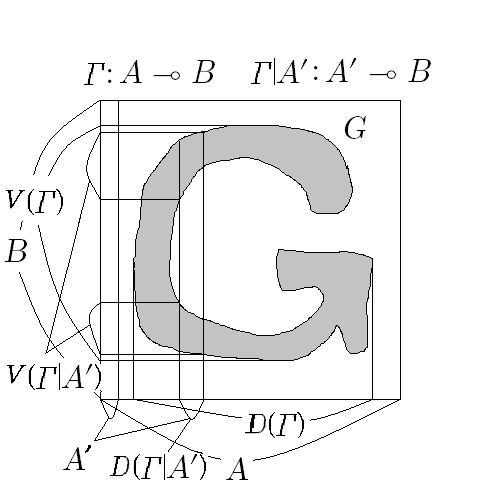
\includegraphics[width=160pt]{1.2.1.a.png}
\end{center}
\begin{thm}
\label{1.2.1.17}
2つの対応たち$\varGamma:A \multimap B$、$\varDelta:A \multimap B$について、$\forall a \in A$に対し、$\varGamma\left( \left\{ a \right\} \right) = \varDelta\left( \left\{ a \right\} \right)$が成り立つならそのときに限り、$\varGamma:A \multimap B = \varDelta:A \multimap B$が成り立つ。
\end{thm}
\begin{proof}
2つの対応たち$\varGamma:A \multimap B$、$\varDelta:A \multimap B$について、$\forall a \in A$に対し、$V\left( \varGamma|\left\{ a \right\} \right) = V\left( \varDelta|\left\{ a \right\} \right)$が成り立つならそのときに限り、2つの対応たち$\varGamma:A \multimap B$、$\varDelta:A \multimap B$をそれぞれ$(A \times B,G)$、$(A \times B,H)$とおけば、次のようになる。
\begin{align*}
&\quad \forall a \in A\left[ V\left( \varGamma|\left\{ a \right\} \right) = V\left( \varDelta|\left\{ a \right\} \right) \right]\\
&\Leftrightarrow \forall a \in A\left[ \left\{ b \in B \middle| \exists a \in \left\{ a \right\}\left[ (a,b) \in G \right] \right\} = \left\{ b \in B \middle| \exists a \in \left\{ a \right\}\left[ (a,b) \in H \right] \right\} \right]\\
&\Leftrightarrow \forall a \in A\left[ \left\{ b \in B \middle| (a,b) \in G \right\} = \left\{ b \in B \middle| (a,b) \in H \right\} \right]
\end{align*}
ここで、外延性の公理より$\forall b \in \left\{ b \in B \middle| (a,b) \in G \right\}$に対し、次式が成り立つ。
\begin{align*}
b \in \left\{ b \in B \middle| (a,b) \in G \right\} \Leftrightarrow b \in \left\{ b \in B \middle| (a,b) \in H \right\}
\end{align*}
分出の公理より次のようになる。
\begin{align*}
&\quad \left( b \in \left\{ b \in B \middle| (a,b) \in G \right\} \Leftrightarrow b \in \left\{ b \in B \middle| (a,b) \in H \right\} \right)\\
&\Leftrightarrow \left( b \in B \land (a,b) \in G \Leftrightarrow b \in B \land (a,b) \in H \right)\\
&\Leftrightarrow \neg\left( \left( b \in B \land (a,b) \in G \right) \vee \left( b \in B \land (a,b) \in H \right) \right) \\ 
&\quad \vee \left( b \in B \land (a,b) \in G \land b \in B \land (a,b) \in H \right)\\
&\Leftrightarrow \neg\left( b \in B \land \left( (a,b) \in G \vee (a,b) \in H \right) \right) \vee \left( b \in B \land (a,b) \in G \land (a,b) \in H \right)\\
&\Leftrightarrow b \notin B \vee \left( (a,b) \notin G \land (a,b) \notin H \right) \vee \left( b \in B \land (a,b) \in G \land (a,b) \in H \right)\\
&\Leftrightarrow \left( b \in B \vee b \notin B \vee \left( (a,b) \notin G \land (a,b) \notin H \right) \right) \\ 
&\quad \land \left( b \notin B \vee \left( (a,b) \in G \land (a,b) \in H \right) \vee \left( (a,b) \notin G \land (a,b) \notin H \right) \right)\\
&\Leftrightarrow \left( \top \vee \left( (a,b) \notin G \land (a,b) \notin H \right) \right) \\
&\quad \land \left( b \notin B \vee \neg\top \vee \left( (a,b) \in G \land (a,b) \in H \right) \vee \left( (a,b) \notin G \land (a,b) \notin H \right) \right)\\
&\Leftrightarrow b \notin B \vee \neg\left( b \in B \land (a,b) \in G \right) \vee \left( (a,b) \in G \land (a,b) \in H \right) \vee \left( (a,b) \notin G \land (a,b) \notin H \right)\\
&\Leftrightarrow \neg\left( b \in B \land (a,b) \in G \right) \vee \neg\left( (a,b) \in G \vee (a,b) \in H \right) \vee \left( (a,b) \in G \land (a,b) \in H \right)\\
&\Leftrightarrow \neg\top \vee \neg\left( (a,b) \in G \vee (a,b) \in H \right) \vee \left( (a,b) \in G \land (a,b) \in H \right)\\
&\Leftrightarrow \neg\left( (a,b) \in G \vee (a,b) \in H \right) \vee \left( (a,b) \in G \land (a,b) \in H \right)\\
&\Leftrightarrow \left( (a,b) \in G \Leftrightarrow (a,b) \in H \right)
\end{align*}
以上より、2つの集合たち$A$、$B$が与えられれば、直積$A \times B$も一意的に存在するので、次のようになる。
\begin{align*}
&\quad \forall a \in A\left[ V\left( \varGamma|\left\{ a \right\} \right) = V\left( \Delta|\left\{ a \right\} \right) \right]\\
&\Leftrightarrow \forall a \in A\forall b \in \left\{ b \in B \middle| (a,b) \in G \right\}\left[ (a,b) \in G \Leftrightarrow (a,b) \in H \right]\\
&\Leftrightarrow \forall a \in A\forall b \in B\left[ (a,b) \in G \Leftrightarrow (a,b) \in H \right]\\
&\Leftrightarrow \forall(a,b) \in A \times B\left[ (a,b) \in G \Leftrightarrow (a,b) \in H \right]
\end{align*}
外延性の公理より次のようになる。
\begin{align*}
\forall a \in A\left[ V\left( \varGamma|\left\{ a \right\} \right) = V\left( \varDelta|\left\{ a \right\} \right) \right] \Leftrightarrow G = H
\end{align*}
その直積$A \times B$が一意的に存在するので、したがって、$A \times B = A \times B$かつ$G = H$が成り立ち、これが成り立つならそのときに限り、$(A \times B,G) = (A \times B,H)$が成り立つ。対応の定義より、よって、2つの対応たち$\varGamma:A \multimap B$、$\varDelta:A \multimap B$について、$\forall a \in A$に対し、$\varGamma\left( \left\{ a \right\} \right) = \varDelta\left( \left\{ a \right\} \right)$が成り立つならそのときに限り、$\varGamma:A \multimap B = \varDelta:A \multimap B$が成り立つ。
\end{proof}
\begin{dfn}
対応$\varGamma:A \multimap B = (A \times B,G)$において、$\forall(a,b) \in A \times B$に対し、$(a,b) \in G \Leftrightarrow (b,a) \in H$となるような対応$(B \times A,H)$も考えられることができ、これをその対応$\varGamma:A \multimap B$の逆対応といい$\varGamma^{- 1}:B \multimap A$と書く。ここで、その対応$\varGamma^{- 1}$によるその集合$B$の部分集合$B'$の像$V\left( \varGamma^{- 1}|B' \right)$をその対応$\varGamma$によるその集合$B'$の原像、逆像などという。
\end{dfn}
\begin{thm}
\label{1.2.1.18}
対応$\varGamma:A \multimap B = (A \times B,G)$において、これの逆対応$\varGamma^{- 1}$が$\varGamma^{- 1}:B \multimap A = (B \times A,H)$と与えられたとき、$H = \left\{ (b,a) \in B \times A \middle| (a,b) \in G \right\}$が成り立つ。
\end{thm}
\begin{proof}
対応$\varGamma:A \multimap B = (A \times B,G)$において、これの逆対応$\varGamma^{- 1}$が$\varGamma^{- 1}:B \multimap A = (B \times A,H)$と与えられたとき、定義より明らかに$H \subseteq B \times A$が成り立つので、$(b,a) \in B \times A$も成り立つ。したがって、$\forall(b,a) \in H$に対し、$(a,b) \in G \Leftrightarrow (b,a) \in H$が成り立つことに注意すれば、
\begin{align*}
(b,a) \in H &\Leftrightarrow (b,a) \in B \times A \land (b,a) \in H\\
&\Leftrightarrow (b,a) \in \left\{ (b,a) \in B \times A \middle| (b,a) \in H \right\}\\
&\Leftrightarrow (b,a) \in \left\{ (b,a) \in B \times A \middle| (a,b) \in G \right\}
\end{align*}
外延性の公理より、よって、次式が成り立つ。
\begin{align*}
H = \left\{ (b,a) \in B \times A \middle| (a,b) \in G \right\}
\end{align*}
\end{proof}
%\hypertarget{ux5199ux50cf}{%
\subsubsection{写像}%\label{ux5199ux50cf}}
\begin{dfn}
対応$f:A \multimap B$について、$\forall a \in A\exists b \in B$に対し、$V\left( f|\left\{ a \right\} \right) = \left\{ b \right\}$が成り立つとき、その対応$f$は写像といい$f:A \rightarrow B$、$A\overset{f}{\rightarrow}B$などと書く。この写像$f:A \rightarrow B$全体の集合を$\mathfrak{F}(A,B)$、$B^{A}$などと書く。このとき、$V\left( f|\left\{ a \right\} \right) = \left\{ b \right\}$のことを、単に、$f(a) = b$と書き、これを明示するとき、その写像$f$を$f:A \rightarrow B;a \mapsto f(a) = b$などと書くときがありその元$b$をその元$a$のその写像$f$による像、その元$a$におけるその写像$f$の値などといいこのことをその写像$f$はその元$a$をその元$b$に写す、その元$a$にその元$b$を対応させるなどという。
\end{dfn}
これらの用語たちは次の図のように該当される。
\begin{center}
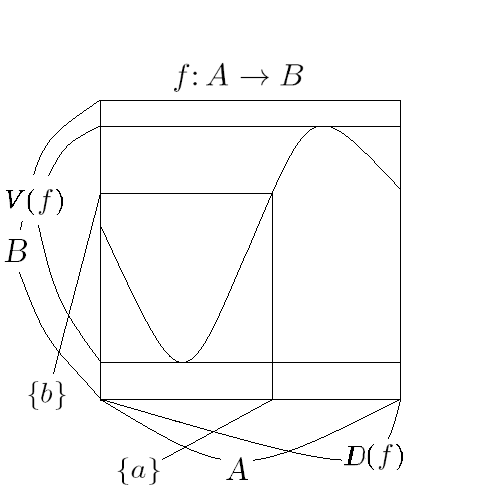
\includegraphics[width=160pt]{1.2.1.b.png}
\end{center}
%\hypertarget{ux4e00ux822cux5316ux3055ux308cux305fux76f4ux7a4d}{%
\subsubsection{一般化された直積}%\label{ux4e00ux822cux5316ux3055ux308cux305fux76f4ux7a4d}}
\begin{dfn}
空でない集合$\varLambda$と集合$A$を用いて、写像$a:\varLambda \rightarrow A$を考えるとき、順序対$\left( a,V(a) \right)$をその集合$\varLambda$によって添数づけられた集合といい、その集合$\varLambda$をその集合$\left( a,V(a) \right)$の添数集合、これの元$\lambda$を添数という。ここで、$a(\lambda)$を$a_{\lambda}$とも書き、その値域$V(a)$は$\left\{ a_{\lambda} \in A \middle| \lambda \in \varLambda \right\}$とも書かれることができる。これをその集合$A$の集合族などといい単に$\left\{ a_{\lambda} \middle| \lambda \in \varLambda \right\}$、$\left\{ a_{\lambda} \right\}_{\lambda \in \varLambda}$などとも書く。
\end{dfn}
\begin{dfn}
次式で定義される集合$\prod_{\lambda \in \varLambda} A_{\lambda}$を空でない集合$\varLambda$によって添数づけられた族$\left\{ A_{\lambda} \right\}_{\lambda \in \varLambda}$の一般化された直積という。なお、集合$\mathfrak{F}\left( \varLambda,\bigcup_{\lambda \in \varLambda} A_{\lambda} \right)$に属する写像$f$を用いた集合$f(\lambda)$が$a_{\lambda}$にあたる。
\begin{align*}
\prod_{\lambda \in \varLambda} A_{\lambda} = \left\{ f \in \mathfrak{F}\left( \varLambda,\bigcup_{\lambda \in \varLambda} A_{\lambda} \right) \middle| \forall\lambda \in \varLambda\left[ f(\lambda) \in A_{\lambda} \right] \right\}
\end{align*}
\end{dfn}
これにより、その写像$f$を$\left( a_{\lambda} \right)_{\lambda \in \varLambda}$と書くことがある。\par
特に、のちに述べるように、$\varLambda = \left\{ \mu,\nu \right\}$、$A_{\mu} = A$、$A_{\nu} = B$、$f(\mu) = a$、$f(\nu) = b$とすれば、その直積$\prod_{\lambda \in \varLambda} A_{\lambda}$、その写像$f$をそれぞれ$A \times B$、$(a,b)$と書くこともある。
\begin{thm}
\label{1.2.1.19}
$f \in \prod_{\lambda \in \varLambda} A_{\lambda}$が成り立つならそのときに限り、写像$f:\varLambda \rightarrow \bigcup_{\lambda \in \varLambda} A_{\lambda}$が与えられ、$\forall\lambda \in \varLambda$に対し、$f(\lambda) \in A_{\lambda}$が成り立つ。
\end{thm}
\begin{proof}
空でない集合$\varLambda$によって添数づけられた族$\left\{ A_{\lambda} \right\}_{\lambda \in \varLambda}$の一般化された直積$\prod_{\lambda \in \varLambda} A_{\lambda}$が与えられたとする。定義より次式が成り立つので、
\begin{align*}
\prod_{\lambda \in \varLambda} A_{\lambda} = \left\{ f \in \mathfrak{F}\left( \varLambda,\bigcup_{\lambda \in \varLambda} A_{\lambda} \right) \middle| \forall\lambda \in \varLambda\left[ f(\lambda) \in A_{\lambda} \right] \right\}
\end{align*}
$f \in \prod_{\lambda \in \varLambda} A_{\lambda}$が成り立つなら、次式が成り立ち、
\begin{align*}
f \in \left\{ f \in \mathfrak{F}\left( \varLambda,\bigcup_{\lambda \in \varLambda} A_{\lambda} \right) \middle| \forall\lambda \in \varLambda\left[ f(\lambda) \in A_{\lambda} \right] \right\}
\end{align*}
分出の公理より写像$f:\varLambda \rightarrow \bigcup_{\lambda \in \varLambda} A_{\lambda}$が与えられ、$\forall\lambda \in \varLambda$に対し、$f(\lambda) \in A_{\lambda}$が成り立つ。\par
逆に、これが成り立つなら、$f \in \mathfrak{F}\left( \varLambda,\bigcup_{\lambda \in \varLambda} A_{\lambda} \right)$かつ、$\forall\lambda \in \varLambda$に対し、$f(\lambda) \in A_{\lambda}$が成り立つので、分出の公理より次式が成り立ち、
\begin{align*}
f \in \left\{ f \in \mathfrak{F}\left( \varLambda,\bigcup_{\lambda \in \varLambda} A_{\lambda} \right) \middle| \forall\lambda \in \varLambda\left[ f(\lambda) \in A_{\lambda} \right] \right\}
\end{align*}
したがって、$f \in \prod_{\lambda \in \varLambda} A_{\lambda}$が成り立つ。
\end{proof}
\begin{thm}
\label{1.2.1.20}
このように定義してもなお、$\varLambda = \left\{ \mu,\nu \right\}$、$A_{\mu} = A$、$A_{\nu} = B$とすれば、$\forall f,g \in A \times B$に対し、$f = g$が成り立つならそのときに限り、$\left( f(\mu),f(\nu) \right) = \left( g(\mu),g(\nu) \right)$が成り立つ。
\end{thm}
\begin{proof}
$\varLambda = \left\{ \mu,\nu \right\}$、$A_{\mu} = A$、$A_{\nu} = B$とすれば、$\forall f,g \in A \times B$に対し、次のようになる。
\begin{align*}
f = g &\Leftrightarrow \forall\lambda \in \varLambda\left[ f(\lambda) = g(\lambda) \right]\\
&\Leftrightarrow f(\mu) = g(\mu) \land f(\nu) = g(\nu)\\
&\Leftrightarrow \left( f(1),f(2) \right) = \left( g(1),g(2) \right)
\end{align*}
\end{proof}
\begin{thm}
\label{1.2.1.21}
空でない集合$\varLambda$によって添数づけられた族$\left\{ A_{\lambda} \right\}_{\lambda \in \varLambda}$の直積$\prod_{\lambda \in \varLambda} A_{\lambda}$において、$\prod_{\lambda \in \varLambda} A_{\lambda} \neq \emptyset$が成り立つなら、$\forall\lambda \in \varLambda$に対し、$A_{\lambda} \neq \emptyset$が成り立つ。
\end{thm}
\begin{proof}
空でない集合$\varLambda$によって添数づけられた族$\left\{ A_{\lambda} \right\}_{\lambda \in \varLambda}$の直積$\prod_{\lambda \in \varLambda} A_{\lambda}$において、$A_{\lambda'} = \emptyset$が成り立つような$\lambda'$が存在するかつ、その直積$\prod_{\lambda \in \varLambda} A_{\lambda}$が空集合でないとすると、直積の定義より$f\left( \lambda' \right) \in A_{\lambda'}$となるような元$f$が存在することになるが、これは$A_{\lambda'} = \emptyset$に矛盾する。したがって、$A_{\lambda'} = \emptyset$が成り立つような$\lambda'$が存在する、即ち、$\exists\lambda' \in \varLambda$に対し、$A_{\lambda'} = \emptyset$が成り立つなら、その直積$\prod_{\lambda \in \varLambda} A_{\lambda}$が空集合である、即ち、$\prod_{\lambda \in \varLambda} A_{\lambda} = \emptyset$が成り立つ。あとは対偶律による。
\end{proof}
%\hypertarget{ux9078ux629eux306eux516cux7406}{%
\subsubsection{選択の公理}%\label{ux9078ux629eux306eux516cux7406}}
\begin{axs}
次式で表される公理を選択の公理、選択公理、選出公理などという。
\begin{align*}
\forall\mathcal{A}\in \mathcal{F\exists}f \in \mathfrak{F}\left( \mathcal{A},\bigcup_{} \mathcal{A} \right)\forall A \in \mathcal{A}\left[ A \neq \emptyset \Rightarrow f(A) \in A \right]
\end{align*}
\end{axs}
これはどの集合$\mathcal{A}$でも、その集合$\mathcal{A}$に属する空でない任意の元$A$に対し、$f(A) \in A$となるような写像$f:\mathcal{A} \rightarrow \bigcup_{} \mathcal{A}$が存在するという意味である。この写像$f$をその集合$\mathcal{A}$の選択写像などという。\footnote{この公理はその写像の具体的な構成が言及されておらず、しばしば直感に反するような命題を導くことがあり、この公理が取り除かれたり、含められたりしたとしても矛盾は生じないと知られているが、この公理が取り除かれると、さまざまな定理たちが証明されることができなくなってしまうため、この公理も含めることが多い…とはいったものの、選択の公理なんか認めん! とかいっていたら数学者の中では異端児扱いされるらしい(?)。}
\begin{thm}
\label{1.2.1.22}
空でない集合$\varLambda$によって添数づけられた族$\left\{ A_{\lambda} \right\}_{\lambda \in \varLambda}$の直積$\prod_{\lambda \in \varLambda} A_{\lambda}$において、$\forall\lambda \in \varLambda$に対し、$A_{\lambda} \neq \emptyset$が成り立つならそのときに限り、$\prod_{\lambda \in \varLambda} A_{\lambda} \neq \emptyset$が成り立つ。
\end{thm}
\begin{proof}
空でない集合$\varLambda$によって添数づけられた族$\left\{ A_{\lambda} \right\}_{\lambda \in \varLambda}$の直積$\prod_{\lambda \in \varLambda} A_{\lambda}$において、$\prod_{\lambda \in \varLambda} A_{\lambda} \neq \emptyset$が成り立つなら、$\forall\lambda \in \varLambda$に対し、$A_{\lambda} \neq \emptyset$が成り立つのであった。逆に、$\forall\lambda \in \varLambda$に対し、$A_{\lambda} \neq \emptyset$が成り立つなら、一般化された直積の定義より、写像$f:\varLambda \rightarrow \left\{ A_{\lambda} \right\}_{\lambda \in \varLambda};f(\lambda) = A_{\lambda}$が存在するのであった。選択の公理よりその集合$\left\{ A_{\lambda} \right\}_{\lambda \in \varLambda}$の選択写像を$g$とすれば、$g\left( A_{\lambda} \right) \in A_{\lambda}$が成り立つ。ここで、写像$h:\varLambda \rightarrow \bigcup_{} \left\{ A_{\lambda} \right\}_{\lambda \in \varLambda} = \bigcup_{\lambda \in \varLambda} A_{\lambda};\lambda \mapsto g\left( A_{\lambda} \right) = g\left( f(\lambda) \right)$を考えると、$h(\lambda) \in A_{\lambda}$が成り立つので、$h \in \prod_{\lambda \in \varLambda} A_{\lambda}$が成り立つ。
\end{proof}
\begin{thebibliography}{50}
    \bibitem{1}
      Rei Frontier Tech Blog. "ZFC公理系について:その1". Hatena Blog. \url{https://tech-blog.rei-frontier.jp/entry/2017/11/02/102042}, (2021-04-01 20:30 閲覧)
    \bibitem{2}
      Rei Frontier Tech Blog. "ZFC公理系について:その2". Hatena Blog. \url{https://tech-blog.rei-frontier.jp/entry/2017/11/09/100000}, (2021-04-01 20:30 閲覧)
    \bibitem{3}
      Rei Frontier Tech Blog. "ZFC公理系について:その3". Hatena Blog. \url{https://tech-blog.rei-frontier.jp/entry/2017/11/16/100000} (2021-04-01 20:30 閲覧)
\end{thebibliography}
\end{document}
    

\clearpage
\documentclass[a4paper]{jsarticle}
\setcounter{section}{2}
\setcounter{subsection}{1}
\usepackage{xr}
\externaldocument{1.2.1}
\usepackage{amsmath,amsfonts,amssymb,array,comment,mathtools,url,docmute}
\usepackage{longtable,booktabs,dcolumn,tabularx,mathtools,multirow,colortbl,xcolor}
\usepackage[dvipdfmx]{graphics}
\usepackage{bmpsize}
\usepackage{amsthm}
\usepackage{enumitem}
\setlistdepth{20}
\renewlist{itemize}{itemize}{20}
\setlist[itemize]{label=•}
\renewlist{enumerate}{enumerate}{20}
\setlist[enumerate]{label=\arabic*.}
\setcounter{MaxMatrixCols}{20}
\setcounter{tocdepth}{3}
\newcommand{\rotin}{\text{\rotatebox[origin=c]{90}{$\in $}}}
\newcommand{\amap}[6]{\text{\raisebox{-0.7cm}{\begin{tikzpicture} 
  \node (a) at (0, 1) {$\textstyle{#2}$};
  \node (b) at (#6, 1) {$\textstyle{#3}$};
  \node (c) at (0, 0) {$\textstyle{#4}$};
  \node (d) at (#6, 0) {$\textstyle{#5}$};
  \node (x) at (0, 0.5) {$\rotin $};
  \node (x) at (#6, 0.5) {$\rotin $};
  \draw[->] (a) to node[xshift=0pt, yshift=7pt] {$\textstyle{\scriptstyle{#1}}$} (b);
  \draw[|->] (c) to node[xshift=0pt, yshift=7pt] {$\textstyle{\scriptstyle{#1}}$} (d);
\end{tikzpicture}}}}
\newcommand{\twomaps}[9]{\text{\raisebox{-0.7cm}{\begin{tikzpicture} 
  \node (a) at (0, 1) {$\textstyle{#3}$};
  \node (b) at (#9, 1) {$\textstyle{#4}$};
  \node (c) at (#9+#9, 1) {$\textstyle{#5}$};
  \node (d) at (0, 0) {$\textstyle{#6}$};
  \node (e) at (#9, 0) {$\textstyle{#7}$};
  \node (f) at (#9+#9, 0) {$\textstyle{#8}$};
  \node (x) at (0, 0.5) {$\rotin $};
  \node (x) at (#9, 0.5) {$\rotin $};
  \node (x) at (#9+#9, 0.5) {$\rotin $};
  \draw[->] (a) to node[xshift=0pt, yshift=7pt] {$\textstyle{\scriptstyle{#1}}$} (b);
  \draw[|->] (d) to node[xshift=0pt, yshift=7pt] {$\textstyle{\scriptstyle{#2}}$} (e);
  \draw[->] (b) to node[xshift=0pt, yshift=7pt] {$\textstyle{\scriptstyle{#1}}$} (c);
  \draw[|->] (e) to node[xshift=0pt, yshift=7pt] {$\textstyle{\scriptstyle{#2}}$} (f);
\end{tikzpicture}}}}
\renewcommand{\thesection}{第\arabic{section}部}
\renewcommand{\thesubsection}{\arabic{section}.\arabic{subsection}}
\renewcommand{\thesubsubsection}{\arabic{section}.\arabic{subsection}.\arabic{subsubsection}}
\everymath{\displaystyle}
\allowdisplaybreaks[4]
\usepackage{vtable}
\theoremstyle{definition}
\newtheorem{thm}{定理}[subsection]
\newtheorem*{thm*}{定理}
\newtheorem{dfn}{定義}[subsection]
\newtheorem*{dfn*}{定義}
\newtheorem{axs}[dfn]{公理}
\newtheorem*{axs*}{公理}
\renewcommand{\headfont}{\bfseries}
\makeatletter
  \renewcommand{\section}{%
    \@startsection{section}{1}{\z@}%
    {\Cvs}{\Cvs}%
    {\normalfont\huge\headfont\raggedright}}
\makeatother
\makeatletter
  \renewcommand{\subsection}{%
    \@startsection{subsection}{2}{\z@}%
    {0.5\Cvs}{0.5\Cvs}%
    {\normalfont\LARGE\headfont\raggedright}}
\makeatother
\makeatletter
  \renewcommand{\subsubsection}{%
    \@startsection{subsubsection}{3}{\z@}%
    {0.4\Cvs}{0.4\Cvs}%
    {\normalfont\Large\headfont\raggedright}}
\makeatother
\makeatletter
\renewenvironment{proof}[1][\proofname]{\par
  \pushQED{\qed}%
  \normalfont \topsep6\p@\@plus6\p@\relax
  \trivlist
  \item\relax
  {
  #1\@addpunct{.}}\hspace\labelsep\ignorespaces
}{%
  \popQED\endtrivlist\@endpefalse
}
\makeatother
\renewcommand{\proofname}{\textbf{証明}}
\usepackage{tikz,graphics}
\usepackage[dvipdfmx]{hyperref}
\usepackage{pxjahyper}
\hypersetup{
 setpagesize=false,
 bookmarks=true,
 bookmarksdepth=tocdepth,
 bookmarksnumbered=true,
 colorlinks=false,
 pdftitle={},
 pdfsubject={},
 pdfauthor={},
 pdfkeywords={}}
\begin{document}
%\hypertarget{ux96c6ux5408ux7b97}{%
\subsection{集合算}%\label{ux96c6ux5408ux7b97}}
%\hypertarget{ux548cux96c6ux5408}{%
\subsubsection{和集合}%\label{ux548cux96c6ux5408}}
\begin{axs*}[公理\ref{和集合の公理}の再掲]
次式で表される公理を和集合の公理という。
\begin{align*}
\forall\mathcal{A}\in \mathcal{F\exists}A \in \mathcal{G\forall}a \in A\left[ a \in A \Leftrightarrow \exists B \in \mathcal{A}[ a \in B] \right]
\end{align*}
\end{axs*}
これにより、その集合$A$はその集合$\mathcal{A}$の元々の元々全体からなる集合となる。定理\ref{1.2.1.4}よりその集合$A$は一意的である。この集合$A$をその集合$\mathcal{A}$に属する集合たち全体の和集合などといい、$\bigcup_{B \in \mathcal{A}} B$、$\bigcup_{} \mathcal{A}$などと書く。特に、$\mathcal{A} =\left\{ A,B \right\}$のとき、和集合$\bigcup_{} \mathcal{A}$を$A \cup B$などと書く。
\begin{thm*}[定理\ref{1.2.1.5}の再掲]
次のことが成り立つのであった。
\begin{itemize}
\item
  $\forall a \in \bigcup_{A \in \mathcal{A}} A$に対し、$a \in \bigcup_{A \in \mathcal{A}} A$が成り立つならそのときに限り、$\exists A \in \mathcal{A}$に対し、$a \in A$が成り立つ。
\item
  $\forall a \in A \cup B$に対し、$a \in A \cup B$が成り立つならそのときに限り、$a \in A$または$a \in B$が成り立つ。
\end{itemize}
\end{thm*}
%\hypertarget{ux7a4dux96c6ux5408}{%
\subsubsection{積集合}%\label{ux7a4dux96c6ux5408}}
\begin{axs*}[公理\ref{分出の公理}の再掲]
対象$a$を変数とする論理式$\varphi(a)$を用いて、次式で表される公理を分出の公理という。
\begin{align*}
\forall A\in \mathcal{F\exists}B \in \mathcal{G\forall}a \in B\left[ a \in B \Leftrightarrow a \in A \land \varphi(a) \right]
\end{align*}
\end{axs*}
定理\ref{1.2.1.8}よりその集合$B$は一意的である。この集合$B$を$\left\{ a \in A \middle| \varphi(a) \right\}$と書きこの記法を内包的記法という。このことを簡単にいえば、次式のようになる。
\begin{align*}
a \in \left\{ a \in A \middle| \varphi(a) \right\} \Leftrightarrow a \in A \land \varphi(a)
\end{align*}
2つの集合たち$A$、$B$を用いた集合$\left\{ a \in A \middle| a \in B \right\}$を$A \cap B$と書き、さらに、2つの集合たち$A$、$\mathcal{A}$を用いた集合$\left\{ a \in A \middle| \forall B\in \mathcal{A}[ a \in B] \right\}$をその集合$\mathcal{A}$に属する集合たち全体の積集合、共通部分などといい、$\bigcap_{A \in \mathcal{A}} A$、$\bigcap_{} \mathcal{A}$などと書く。\par
さらに、2つの集合たち$A$、$B$を用いた集合$\left\{ a \in A \middle| a \notin B \right\}$をその集合$A$に対するその集合$B$の補集合といい$A \setminus B$などと書き、特に、その集合$A$が明らかなとき、その集合$A$を全体集合などといいこの場合のその集合$A$に対するその集合$B$の補集合を$B^{c}$などと書く。定理\ref{1.2.1.9}より$A \setminus B = A \cap B^{c}$が成り立つのであった。\par
その集合$\mathcal{A}$に属する集合たち全体の和集合$\bigcup_{} \mathcal{A}$のうち、$\forall A,B \in \mathcal{A}$に対し、$A \cap B = \emptyset$が成り立つようなものをその集合$\mathcal{A}$に属する集合たち全体の直和などといい$\bigsqcup_{A \in \mathcal{A}} A$、$\bigsqcup_{} \mathcal{A}$などと書く。さらに、このような集合$\mathcal{A}$を互いに素であるという。特に、$\mathcal{A} =\left\{ A,B \right\}$のとき、$A \sqcup B$などとも書く。
\begin{thm*}[定理\ref{1.2.1.10}の再掲]
積集合について次のことが成り立つ。
\begin{itemize}
\item
  $\forall a \in \bigcap_{A \in \mathcal{A}} A$に対し、$a \in \bigcap_{A \in \mathcal{A}} A$が成り立つならそのときに限り、$\forall A \in \mathcal{A}$に対し、$a \in A$が成り立つ。
\item
  $\forall a \in A \cap B$に対し、$a \in A \cap B$が成り立つならそのときに限り、$a \in A$かつ$a \in B$が成り立つ。
\item
  空集合$\emptyset$に属する元があることは偽である、即ち、$\forall A\in \mathcal{F}$に対し、$\emptyset = \left\{ a \in A \middle| \bot \right\}$が成り立つ。
\end{itemize}
\end{thm*}
%\hypertarget{ux548cux96c6ux5408ux3068ux7a4dux96c6ux5408ux306eux6027ux8cea}{%
\subsubsection{和集合と積集合の性質}%\label{ux548cux96c6ux5408ux3068ux7a4dux96c6ux5408ux306eux6027ux8cea}}
\begin{thm}
\label{1.2.2.1}
3つの集合たち$A$、$B$、$C$について次式たちが成り立つ。
\begin{longtable}[c]{|c|c|}
\hline
名称 & 式 \\
\hline \hline
& $A \subseteq A \cup B$ \\
& $A \cap B \subseteq A$ \\
\hline
& $A \subseteq C \land B \subseteq C \Leftrightarrow A \cup B \subseteq C$ \\
& $C \subseteq A \land C \subseteq B \Leftrightarrow C \subseteq A \cap B$ \\
\hline
巾等律 & \hspace{-0.5em}\begin{tabular}{c}
  $A \cup A = A$ \\
  $A \cap A = A$ 
\end{tabular}\\
\hline
交換律 & \hspace{-0.5em}\begin{tabular}{c}
  $A \cup B = B \cup A$ \\
  $A \cap B = B \cap A$ 
\end{tabular}\\
\hline
結合律 & \hspace{-0.5em}\begin{tabular}{c}
  $(A \cup B) \cup C = A \cup (B \cup C) $\\
  $(A \cap B) \cap C = A \cap (B \cap C)$ 
\end{tabular}\\
\hline
& $A \subseteq B \Leftrightarrow A \cup B = B $\\
& $A \subseteq B \Leftrightarrow A \cap B = A$ \\
\hline
& $A \subseteq B \Rightarrow A \cup C \subseteq B \cup C$ \\
& $A \subseteq B \Rightarrow A \cap C \subseteq B \cap C$ \\
\hline
& $\emptyset \cup A = A$ \\
& $\emptyset \cap A = \emptyset$ \\
\hline
分配律 & \hspace{-0.5em}\begin{tabular}{c}
  $A \cup (B \cap C) = (A \cup B) \cap (A \cup C) $\\
  $A \cap (B \cup C) = (A \cap B) \cup (A \cap C)$ 
\end{tabular}\\
\hline
吸収律 & \hspace{-0.5em}\begin{tabular}{c}
  $A \cup (A \cap B) = A$\\
  $A \cap (A \cup B) = A$ 
\end{tabular}\\
\hline
\end{longtable}
\end{thm}
\begin{proof}
3つの集合たち$A$、$B$、$C$について、$\forall a \in A$に対し、次のようになり、
\begin{align*}
a \in A &\Rightarrow a \in A \vee a \in B\\
&\Leftrightarrow a \in A \cup B 
\end{align*}
よって、$A \subseteq A \cup B$が成り立つ。\par
$\forall a \in A \cap B$に対し、次のようになり、
\begin{align*}
a \in A \cap B &\Leftrightarrow a \in A \land a \in B\\
&\Rightarrow a \in A
\end{align*}
よって、$A \cap B \subseteq A$が成り立つ。\par
$\forall a \in A \cup B$に対し、次のようになり、
\begin{align*}
(a \in A \Rightarrow a \in C) \land (a \in B \Rightarrow a \in C) &\Leftrightarrow (a \notin A \vee a \in C) \land (a \notin B \vee a \in C)\\
&\Leftrightarrow (a \notin A \land a \notin B) \vee a \in C\\
&\Leftrightarrow \neg(a \in A \vee a \in B) \vee a \in C\\
&\Leftrightarrow a \in A \cup B \Rightarrow a \in C
\end{align*}
よって、$A \subseteq C \land B \subseteq C \Leftrightarrow A \cup B \subseteq C$が成り立つ。\par
$\forall a \in C$に対し、次のようになり、
\begin{align*}
(a \in C \Rightarrow a \in A) \land (a \in C \Rightarrow a \in B) &\Leftrightarrow (a \notin C \vee a \in A) \land (a \notin C \vee a \in B)\\
&\Leftrightarrow a \notin C \vee (a \in A \land a \in B)\\
&\Leftrightarrow a \in C \Rightarrow a \in A \cap B
\end{align*}
よって、$C \subseteq A \land C \subseteq B \Leftrightarrow C \subseteq A \cap B$が成り立つ。\par
論理和と論理積の巾等律と交換律、結合律、分配律が成り立つのあったので、明らかに次式たちが成り立つ。
\begin{align*}
A \cup A &= A\\
A \cap A &= A\\
A \cup B &= B \cup A\\
A \cap B &= B \cap A\\
(A \cup B) \cup C &= A \cup (B \cup C)\\
(A \cap B) \cap C &= A \cap (B \cap C)\\
A \cup (B \cap C) &= (A \cup B) \cap (A \cup C)\\
A \cap (B \cup C) &= (A \cap B) \cup (A \cap C)
\end{align*}
$\forall a \in A$に対し、次のようになり、
\begin{align*}
a \in A &\Rightarrow a \in B \Leftrightarrow a \notin A \vee a \in B\\
&\Leftrightarrow (a \notin A \vee a \in B) \land \top\\
&\Leftrightarrow (a \notin A \vee a \in B) \land (a \in A \vee a \notin A \vee a \in B)\\
&\Leftrightarrow a \notin A \vee a \in B \vee (a \in A \land a \in B)\\
&\Leftrightarrow \left( a \notin A \vee a \in B \vee (a \in A \land a \in B) \right) \land \top\\
&\Leftrightarrow \left( a \notin A \vee a \in B \vee (a \in A \land a \in B) \right) \\
&\quad \land \left( (a \in A \land a \in B) \vee a \in B \vee a \notin B \right)\\
&\Leftrightarrow (a \in A \land a \in B) \vee a \in B \vee (a \notin A \land a \notin B)\\
&\Leftrightarrow \neg(a \in A \vee a \in B) \vee \left( (a \in A \vee a \in B) \land a \in B \right)\\
&\Leftrightarrow \neg(a \in A \vee a \in B \vee a \in B) \\
&\quad \vee \left( (a \in A \vee a \in B) \land a \in B \right)\\
&\Leftrightarrow (a \in A \vee a \in B \Leftrightarrow a \in B)\\
&\Leftrightarrow (a \in A \cup B \Leftrightarrow a \in B)
\end{align*}
よって、$A \subseteq B \Leftrightarrow A \cup B = B$が成り立つ。\par
$\forall a \in A$に対し、次のようになり、
\begin{align*}
a \in A \Rightarrow a \in B &\Leftrightarrow a \notin A \vee a \in B \\
&\Leftrightarrow (a \notin A \vee a \in B) \land \top\\
&\Leftrightarrow (a \notin A \vee a \in B) \land (a \in A \vee a \notin A) \\
&\Leftrightarrow a \notin A \vee (a \in A \land a \in B)\\
&\Leftrightarrow \left( a \notin A \vee (a \in A \land a \in B) \right) \land \top\\
&\Leftrightarrow \left( a \notin A \vee (a \in A \land a \in B) \right) \\
&\quad \land \left( \neg(a \in A \land a \in B) \vee (a \in A \land a \in B) \right)\\
&\Leftrightarrow (a \in A \land a \in B) \vee \left( \neg(a \in A \land a \in B) \land a \notin A \right)\\
&\Leftrightarrow (a \in A \land a \in B) \vee \neg\left( (a \in A \land a \in B) \vee a \in A \right)\\
&\Leftrightarrow (a \in A \land a \in B \Leftrightarrow a \in A)\\
&\Leftrightarrow (a \in A \cap B \Leftrightarrow a \in A)
\end{align*}
よって、$A \subseteq B \Leftrightarrow A \cap B = A$が成り立つ。\par
$\forall a \in A$に対し、次のようになり、
\begin{align*}
a \in A \Rightarrow a \in B &\Leftrightarrow a \notin A \vee a \in B\\
&\Rightarrow a \notin A \vee a \in B \vee a \in C\\
&\Leftrightarrow (a \notin A \vee a \in B \vee a \in C) \land \top\\
&\Leftrightarrow (a \notin A \vee a \in B \vee a \in C) \\
&\quad \land (a \in B \vee a \in C \vee a \notin C)\\
&\Leftrightarrow (a \notin A \land a \notin C) \vee a \in B \vee a \in C\\
&\Leftrightarrow (a \in A \vee a \in C) \Rightarrow (a \in B \vee a \in C)\\
&\Leftrightarrow a \in A \cup C \Rightarrow a \in B \cup C
\end{align*}
よって、$A \subseteq B \Rightarrow A \cup C \subseteq B \cup C$が成り立つ。\par
$\forall a \in A$に対し、次のようになり、
\begin{align*}
a \in A \Rightarrow a \in B &\Leftrightarrow a \notin A \vee a \in B\\
&\Rightarrow a \notin A \vee a \in B \vee a \notin C\\
&\Leftrightarrow (a \notin A \vee a \in B \vee a \notin C) \land \top\\
&\Leftrightarrow (a \notin A \vee a \in B \vee a \notin C) \\
&\quad \land (a \notin A \vee a \in C \vee a \notin C)\\
&\Leftrightarrow a \notin A \vee a \notin C \vee (a \in B \land a \in C)\\
&\Leftrightarrow (a \in A \land a \in C) \Rightarrow (a \in B \land a \in C)\\
&\Leftrightarrow (a \in A \cap C) \Rightarrow (a \in B \cap C)
\end{align*}
よって、$A \subseteq B \Rightarrow A \cap C \subseteq B \cap C$が成り立つ。\par
また、$a \in \emptyset$が成り立つならそのときに限り、$\emptyset = \left\{ a \in A \middle| \bot \right\}$が成り立つのであったので、$a \in A \land \bot$が成り立ち、したがって、$\bot$が成り立つ。\par
$\forall a \in A$に対し、次のようになり、
\begin{align*}
a \in \emptyset \cup A &\Leftrightarrow a \in \emptyset \vee a \in A \\
&\Leftrightarrow \bot \vee a \in A \\
&\Leftrightarrow a \in A
\end{align*}
よって、$\emptyset \cup A \Leftrightarrow A$が成り立つ。\par
$\forall a \in A$に対し、次のようになり、
\begin{align*}
a \in \emptyset \cap A &\Leftrightarrow a \in \emptyset \land a \in A \\
&\Leftrightarrow \bot \land a \in A \\
&\Leftrightarrow \bot \Leftrightarrow a \in \emptyset
\end{align*}
よって、$\emptyset \cap A \Leftrightarrow \emptyset$が成り立つ。\par
$\forall a \in A$に対し、次のようになり、
\begin{align*}
\left( a \in A \cup (A \cap B) \Leftrightarrow a \in A \right) &\Leftrightarrow \left( a \in A \vee (a \in A \land a \in B) \Leftrightarrow a \in A \right)\\
&\Leftrightarrow \neg\left( a \in A \vee (a \in A \land a \in B) \vee a \in A \right) \\
&\quad \vee \left( \left( a \in A \vee (a \in A \land a \in B) \right) \land a \in A \right)\\
&\Leftrightarrow \neg\left( a \in A \vee (a \in A \land a \in B) \right) \\
&\quad \vee a \in A \vee (a \in A \land a \in B)\\
&\Leftrightarrow \left( a \notin A \vee \neg(a \in A \land a \in B) \right) \\
&\quad \vee a \in A \vee (a \in A \land a \in B)\\
&\Leftrightarrow \left( a \notin A \vee a \in A \vee (a \in A \land a \in B) \right) \\
&\quad \vee \left( \neg(a \in A \land a \in B) \vee a \in A \vee (a \in A \land a \in B) \right)\\
&\Leftrightarrow \top \vee \top \Leftrightarrow \top
\end{align*}
よって、$A \cup (A \cap B) = A$が成り立つ。\par
$\forall a \in A$に対し、次のようになり、
\begin{align*}
\left( a \in A \cap (A \cup B) \Leftrightarrow a \in A \right) &\Leftrightarrow \left( a \in A \land (a \in A \vee a \in B) \Leftrightarrow a \in A \right)\\
&\Leftrightarrow \neg\left( \left( a \in A \land (a \in A \vee a \in B) \right) \vee a \in A \right) \\
&\quad \vee \left( a \in A \land (a \in A \vee a \in B) \land a \in A \right)\\
&\Leftrightarrow \left( \neg\left( a \in A \land (a \in A \vee a \in B) \right) \land a \notin A \right) \\
&\quad \vee \left( a \in A \land (a \in A \vee a \in B) \right)\\
&\Leftrightarrow \left( \neg\left( a \in A \land (a \in A \vee a \in B) \right) \right. \\
&\quad \left. \vee \left( a \in A \land (a \in A \vee a \in B) \right) \right) \\
&\quad \land \left( a \notin A \vee \left( a \in A \land (a \in A \vee a \in B) \right) \right)\\
&\Leftrightarrow \top \land (a \notin A \vee a \in A) \land (a \notin A \vee a \in A \vee a \in B)\\
&\Leftrightarrow \top \land \top \land \top \Leftrightarrow \top
\end{align*}
よって、$A \cap (A \cup B) = A$が成り立つ。
\end{proof}
\begin{thm}
\label{1.2.2.2}
より一般的に次式が成り立つ。なお、集合$\mathcal{A}$の元の1つを$\overline{A}$とおいた。
\begin{longtable}[c]{|c|c|}
\hline
名称 & 式 \\
\hline \hline
& \hspace{-0.5em}\begin{tabular}{c}
  $\overline{A} \subseteq \bigcup_{A \in \mathcal{A}} A $\\
  $\bigcap_{A \in \mathcal{A}} A \subseteq \overline{A}$ \end{tabular} \\
\hline
巾等律 & \hspace{-0.5em}\begin{tabular}{c}
  $\bigcup_{A \in \mathcal{A}} A = \overline{A}\ \mathrm{if}\ \forall A \in \mathcal{A}\left[ A = \overline{A} \right] $\\
  $\bigcap_{A \in \mathcal{A}} A = \overline{A}\ \mathrm{if}\ \forall A \in \mathcal{A}\left[ A = \overline{A} \right]$ 
\end{tabular}\\
\hline
分配律 & \hspace{-0.5em}\begin{tabular}{c}
  $\bigcup_{A \in \mathcal{A}} A \cap B = \bigcup_{A \in \mathcal{A}} (A \cap B) $\\
  $\bigcap_{A \in \mathcal{A}} A \cup B = \bigcap_{A \in \mathcal{A}} (A \cup B)$ 
\end{tabular}\\
\hline
\multirow{2}{*}{de Morgan律} & \hspace{-0.5em}\begin{tabular}{c}
  $B \setminus \bigcup_{A \in \mathcal{A}} A = \bigcap_{A \in \mathcal{A}} (B \setminus A) $\\
  $B \setminus \bigcap_{A \in \mathcal{A}} A = \bigcup_{A \in \mathcal{A}} (B \setminus A)$ 
\end{tabular}\\ \cline{2-2}
& \hspace{-0.5em}\begin{tabular}{c}
  $\left( \bigcup_{A \in \mathcal{A}} A \right)^{c} = \bigcap_{A \in \mathcal{A}} A^{c}$ \\
  $\left( \bigcap_{A \in \mathcal{A}} A \right)^{c} = \bigcup_{A \in \mathcal{A}} A^{c}$ 
\end{tabular}\\
\hline
\end{longtable}
\end{thm}
\begin{proof}
集合$\mathcal{A}$の元の1つを$\overline{A}$とおく。このとき、$\forall a \in \overline{A}$に対し、次のようになり、
\begin{align*}
a \in \overline{A} \Rightarrow \exists A \in \mathcal{A}[ a \in A]
\end{align*}
したがって、次式が成り立つ。
\begin{align*}
\overline{A} \subseteq \bigcup_{A \in \mathcal{A}} A
\forall A \in \mathcal{A}[ a \in A] \Rightarrow a \in \overline{A}
\end{align*}
したがって、次式が成り立つ。
\begin{align*}
\bigcap_{A \in \mathcal{A}} A \subseteq \overline{A}
\end{align*}
$\forall A \in \mathcal{A}$に対し、$A = \overline{A}$が成り立つとき、次のようになり、
\begin{align*}
\exists A \in \mathcal{A}[ a \in A] &\Leftrightarrow \exists A \in \mathcal{A}\left[ a \in \overline{A} \right] \Leftrightarrow a \in \overline{A}\\
\forall A \in \mathcal{A}[ a \in A] &\Leftrightarrow \forall A \in \mathcal{A}\left[ a \in \overline{A} \right] \Leftrightarrow a \in \overline{A}
\end{align*}
したがって、次式が成り立つ。
\begin{align*}
\bigcup_{A \in \mathcal{A}} A &= \overline{A}\ \mathrm{if}\ \forall A \in \mathcal{A}\left[ A = \overline{A} \right]\\
\bigcap_{A \in \mathcal{A}} A &= \overline{A}\ \mathrm{if}\ \forall A \in \mathcal{A}\left[ A = \overline{A} \right]
\end{align*}
$\forall a \in \bigcup_{A \in \mathcal{A}} A \cap B$に対し、次のようになり、
\begin{align*}
a \in \bigcup_{A \in \mathcal{A}} A \cap B &\Leftrightarrow \exists A \in \mathcal{A}[ a \in A] \land a \in B\\
&\Leftrightarrow \exists A \in \mathcal{A}[ a \in A \land a \in B]\\
&\Leftrightarrow \exists A \in \mathcal{A}[ a \in A \cap B]\\
&\Leftrightarrow a \in \bigcup_{A \in \mathcal{A}} (A \cap B)\\
a \in \bigcap_{A \in \mathcal{A}} A \cup B &\Leftrightarrow \forall A \in \mathcal{A}[ a \in A] \vee a \in B\\
&\Leftrightarrow \forall A \in \mathcal{A}[ a \in A \vee a \in B]\\
&\Leftrightarrow \forall A \in \mathcal{A}[ a \in A \cup B]\\
&\Leftrightarrow a \in \bigcap_{A \in \mathcal{A}} (A \cup B)
\end{align*}
したがって、次式が成り立つ。
\begin{align*}
\bigcup_{A \in \mathcal{A}} A \cap B &= \bigcup_{A \in \mathcal{A}} (A \cap B)\\
\bigcap_{A \in \mathcal{A}} A \cup B &= \bigcap_{A \in \mathcal{A}} (A \cup B)
\end{align*}
$\forall a \in B \setminus \bigcup_{A \in \mathcal{A}} A$に対し、次のようになり、
\begin{align*}
a \in B \setminus \bigcup_{A \in \mathcal{A}} A &\Leftrightarrow a \in B \land a \notin \bigcup_{A \in \mathcal{A}} A\\
&\Leftrightarrow a \in B \land \neg\exists A \in \mathcal{A}[ a \in A]\\
&\Leftrightarrow a \in B \land \forall A \in \mathcal{A}[ a \notin A]\\
&\Leftrightarrow \forall A \in \mathcal{A}[ a \in B \land a \notin A]\\
&\Leftrightarrow \forall A \in \mathcal{A}[ a \in B \setminus A]\\
&\Leftrightarrow a \in \bigcap_{A \in \mathcal{A}} (B \setminus A)
\end{align*}
したがって、次式が成り立つ。
\begin{align*}
B \setminus \bigcup_{A \in \mathcal{A}} A = \bigcap_{A \in \mathcal{A}} (B \setminus A)
\end{align*}
$\forall a \in B \setminus \bigcap_{A \in \mathcal{A}} A$に対し、次のようになり、
\begin{align*}
a \in B \setminus \bigcap_{A \in \mathcal{A}} A &\Leftrightarrow a \in B \land a \notin \bigcap_{A \in \mathcal{A}} A\\
&\Leftrightarrow a \in B \land \neg\forall A \in \mathcal{A}[ a \in A]\\
&\Leftrightarrow a \in B \land \exists A \in \mathcal{A}[ a \notin A]\\
&\Leftrightarrow \exists A \in \mathcal{A}[ a \in B \land a \notin A]\\
&\Leftrightarrow \exists A \in \mathcal{A}[ a \in B \setminus A]\\
&\Leftrightarrow a \in \bigcup_{A \in \mathcal{A}} (B \setminus A)
\end{align*}
したがって、次式が成り立つ。
\begin{align*}
B \setminus \bigcap_{A \in \mathcal{A}} A = \bigcup_{A \in \mathcal{A}} (B \setminus A)
\end{align*}
\end{proof}
%\hypertarget{ux5deeux96c6ux5408ux306eux6027ux8cea}{%
\subsubsection{差集合の性質}%\label{ux5deeux96c6ux5408ux306eux6027ux8cea}}
\begin{thm}
\label{1.2.2.3}
4つの集合たち$A$、$B$、$C$、$U$について次式たちが成り立つ。
\begin{longtable}[c]{|c|c|}
\hline
名称 & 式\\
\hline \hline
& \hspace{-0.5em}\begin{tabular}{c}
  $(A \cup B) \setminus C = A \setminus C \cup B \setminus C$\\
  $(A \cap B) \setminus C = A \setminus C \cap B \setminus C$ \end{tabular}\\
\hline
\multirow{2}{*}{de Morgan律} & \hspace{-0.5em}\begin{tabular}{c}
  $A \setminus (B \cup C) = A \setminus B \cap A \setminus C$\\
  $A \setminus (B \cap C) = A \setminus B \cup A \setminus C$ \end{tabular} \\ \cline{2-2}
& \hspace{-0.5em}\begin{tabular}{c}
  $(A \cup B)^{c} = A^{c} \cap B^{c}$\\
  $(A \cap B)^{c} = A^{c} \cup B^{c}$ \end{tabular} \\
\hline
& \hspace{-0.5em}\begin{tabular}{c}
  $A \cup (B \setminus C) = (A \cup B) \setminus (C \setminus A) $\\
  $A \cap (B \setminus C) = (A \cap B) \setminus C$ \end{tabular} \\ \cline{2-2}
& \hspace{-0.5em}\begin{tabular}{c}
  $A \cup B^{c} = (B \setminus A)^{c} $ \\
  $A \cap B^{c} = A \setminus B$ \end{tabular} \\
\hline
& \hspace{-0.5em}\begin{tabular}{c}
  $(A \setminus B) \setminus C = A \setminus (B \cup C) $\\
  $A \setminus (B \setminus C) = A \setminus B \cup (A \cap C) $\end{tabular} \\
\hline
& \hspace{-0.5em}\begin{tabular}{c}
  $A^{c} \setminus B = (A \cup B)^{c} $\\
  $(A \setminus B)^{c} = A^{c} \cup B$ \end{tabular} \\
\hline
& $A \setminus \emptyset = A$ \\
\hline
\multirow{2}{*}{de Morgan律} & \hspace{-0.5em}\begin{tabular}{c}
  $\emptyset \setminus A = \emptyset $ \\
  $A \setminus A = \emptyset$ \end{tabular}\\ \cline{2-2}
& \hspace{-0.5em}\begin{tabular}{c}
  $\emptyset^{c} = U$ \\
  $U^{c} = \emptyset$ \end{tabular} \\
\hline
& \hspace{-0.5em}\begin{tabular}{c}
  $B \cup (A \setminus B) = A \cup B$\\
  $A \setminus (A \setminus B) = A \cap B$\\
  $B \cap (A \setminus B) = \emptyset$ \end{tabular} \\ \cline{2-2}
& \hspace{-0.5em}\begin{tabular}{c}
  $A \cup A^{c} = U$\\
  $A^{cc} = A$\\
  $A \cap A^{c} = \emptyset$ \end{tabular} \\
\hline
& $B \subseteq C \Leftrightarrow A \setminus B \supseteq A \setminus C$ \\ \cline{2-2}
& $A \subseteq B \Leftrightarrow A^{c} \supseteq B^{c}$ \\
\hline
\end{longtable}
\end{thm}
\begin{proof}
3つの集合たち$A$、$B$、$C$について、$\forall a \in (A \cup B) \setminus C$に対し、次のようになり、
\begin{align*}
a \in (A \cup B) \setminus C &\Leftrightarrow a \in A \cup B \land a \notin C\\
&\Leftrightarrow (a \in A \vee a \in B) \land a \notin C\\
&\Leftrightarrow (a \in A \land a \notin C) \vee (a \in B \land a \notin C)\\
&\Leftrightarrow a \in A \setminus C \vee a \in B \setminus C\\
&\Leftrightarrow a \in A \setminus C \cup B \setminus C
\end{align*}
よって、$(A \cup B) \setminus C = A \setminus C \cup B \setminus C$が成り立つ。\par
$\forall a \in (A \cap B) \setminus C$に対し、次のようになり、
\begin{align*}
a \in (A \cap B) \setminus C &\Leftrightarrow a \in A \cap B \land a \notin C\\
&\Leftrightarrow a \in A \land a \in B \land a \notin C\\
&\Leftrightarrow (a \in A \land a \notin C) \land (a \in B \land a \notin C)\\
&\Leftrightarrow a \in A \setminus C \land a \in B \setminus C\\
&\Leftrightarrow a \in A \setminus C \cap B \setminus C
\end{align*}
よって、$(A \cap B) \setminus C = A \setminus C \cap B \setminus C$が成り立つ。\par
$\forall a \in A \setminus (B \cup C)$に対し、次のようになり、
\begin{align*}
a \in A \setminus (B \cup C) &\Leftrightarrow a \in A \land a \notin B \cup C\\
&\Leftrightarrow a \in A \land \neg(a \in B \vee a \in C)\\
&\Leftrightarrow a \in A \land a \notin B \land a \notin C\\
&\Leftrightarrow (a \in A \land a \notin B) \land (a \in A \land a \notin C)\\
&\Leftrightarrow a \in A \setminus B \land a \in A \setminus C\\
&\Leftrightarrow a \in A \setminus B \cap A \setminus C
\end{align*}
よって、$A \setminus (B \cup C) = A \setminus B \cap A \setminus C$が成り立つ。\par
$\forall a \in A \setminus (B \cap C)$に対し、次のようになり、
\begin{align*}
a \in A \setminus (B \cap C) &\Leftrightarrow a \in A \land a \notin B \cap C\\
&\Leftrightarrow a \in A \land \neg(a \in B \land a \in C)\\
&\Leftrightarrow a \in A \land (a \notin B \vee a \notin C)\\
&\Leftrightarrow (a \in A \land a \notin B) \vee (a \in A \land a \notin C)\\
&\Leftrightarrow a \in A \setminus B \vee a \in A \setminus C\\
&\Leftrightarrow a \in A \setminus B \cup A \setminus C
\end{align*}
よって、$A \setminus (B \cap C) = A \setminus B \cup A \setminus C$が成り立つ。\par
$\forall a \in A \cup (B \setminus C)$に対し、次のようになり、
\begin{align*}
a \in A \cup (B \setminus C) &\Leftrightarrow a \in A \vee a \in B \setminus C\\
&\Leftrightarrow a \in A \vee (a \in B \land a \notin C)\\
&\Leftrightarrow (a \in A \vee a \in B) \land (a \in A \vee a \notin C)\\
&\Leftrightarrow (a \in A \vee a \in B) \land \neg(a \notin A \land a \in C)\\
&\Leftrightarrow a \in A \cup B \land a \notin C \setminus A\\
&\Leftrightarrow a \in (A \cup B) \setminus (C \setminus A)
\end{align*}
よって、$A \cup (B \setminus C) = (A \cup B) \setminus (C \setminus A)$が成り立つ。\par
$\forall a \in A \cap (B \setminus C)$に対し、次のようになり、
\begin{align*}
a \in A \cap (B \setminus C) &\Leftrightarrow a \in A \land a \in B \setminus C\\
&\Leftrightarrow a \in A \land a \in B \land a \notin C\\
&\Leftrightarrow a \in A \cap B \land a \notin C\\
&\Leftrightarrow a \in (A \cap B) \setminus C
\end{align*}
よって、$A \cap (B \setminus C) = (A \cap B) \setminus C$が成り立つ。\par
$\forall a \in (A \setminus B) \setminus C$に対し、次のようになり、
\begin{align*}
a \in (A \setminus B) \setminus C &\Leftrightarrow a \in A \setminus B \land a \notin C\\
&\Leftrightarrow a \in A \land a \notin B \land a \notin C\\
&\Leftrightarrow a \in A \land \neg(a \in B \vee a \in C)\\
&\Leftrightarrow a \in A \land a \notin B \cup C\\
&\Leftrightarrow a \in A \setminus (B \cup C)
\end{align*}
よって、$(A \setminus B) \setminus C = A \setminus (B \cup C)$が成り立つ。\par
$\forall a \in A \setminus (B \setminus C)$に対し、次のようになり、
\begin{align*}
a \in A \setminus (B \setminus C) &\Leftrightarrow a \in A \land a \notin B \setminus C\\
&\Leftrightarrow a \in A \land \neg(a \in B \land a \notin C)\\
&\Leftrightarrow a \in A \land (a \notin B \vee a \in C)\\
&\Leftrightarrow (a \in A \land a \notin B) \vee (a \in A \land a \in C)\\
&\Leftrightarrow a \in A \setminus B \vee a \in A \cap C\\
&\Leftrightarrow a \in (A \setminus B) \cup (A \cap C)
\end{align*}
よって、$A \setminus (B \setminus C) = A \setminus B \cup (A \cap C)$が成り立つ。\par
$\forall a \in A \setminus \emptyset$に対し、次のようになり、
\begin{align*}
a \in A \setminus \emptyset &\Leftrightarrow a \in A \land a \notin \emptyset \\ 
&\Leftrightarrow a \in A \land \top \\
&\Leftrightarrow a \in A
\end{align*}
よって、$A \setminus \emptyset = A$が成り立つ。\par
$\forall a \in \emptyset \setminus A$に対し、次のようになり、
\begin{align*}
a \in \emptyset \setminus A &\Leftrightarrow a \in \emptyset \land a \notin A \\
&\Leftrightarrow \bot \land a \notin A \\
&\Leftrightarrow \bot \Leftrightarrow a \in \emptyset
\end{align*}
よって、$\emptyset \setminus A = \emptyset$が成り立つ。\par
$\forall a \in A \setminus A$に対し、次のようになり、
\begin{align*}
a \in A \setminus A &\Leftrightarrow a \in A \land a \notin A \\
&\Leftrightarrow \bot \Leftrightarrow a \in \emptyset
\end{align*}
外延性の公理より、よって、$A \setminus A = \emptyset$が成り立つ。\par
$\forall a \in B \cup (A \setminus B)$に対し、次のようになり、
\begin{align*}
a \in B \cup (A \setminus B) &\Leftrightarrow a \in B \vee a \in A \setminus B\\
&\Leftrightarrow a \in B \vee (a \in A \land a \notin B)\\
&\Leftrightarrow (a \in B \vee a \in A) \land (a \in B \vee a \notin B)\\
&\Leftrightarrow (a \in A \cup B) \land \top\\
&\Leftrightarrow a \in A \cup B
\end{align*}
よって、$B \cup (A \setminus B) = A \cup B$が成り立つ。\par
$\forall a \in A \setminus (A \setminus B)$に対し、次のようになり、
\begin{align*}
a \in A \setminus (A \setminus B) &\Leftrightarrow a \in A \land a \notin A \setminus B\\
&\Leftrightarrow a \in A \land \neg(a \in A \land a \notin B)\\
&\Leftrightarrow a \in A \land (a \notin A \vee a \in B)\\
&\Leftrightarrow (a \in A \land a \notin A) \vee (a \in A \land a \in B)\\
&\Leftrightarrow \bot \vee a \in A \cap B\\
&\Leftrightarrow a \in A \cap B
\end{align*}
よって、$A \setminus (A \setminus B) = A \cap B$が成り立つ。\par
$\forall a \in B \cap (A \setminus B)$に対し、次のようになり、
\begin{align*}
a \in B \cap (A \setminus B) &\Leftrightarrow a \in B \land a \in A \setminus B\\
&\Leftrightarrow a \in B \land a \in A \land a \notin B\\
&\Leftrightarrow a \in A \land \bot \Leftrightarrow \bot \Leftrightarrow a \in \emptyset
\end{align*}
よって、$B \cap (A \setminus B) = \emptyset$が成り立つ。\par
$\forall a \in B$に対し、次のようになり、
\begin{align*}
a \in B \Rightarrow a \in C &\Leftrightarrow a \notin B \Leftarrow a \notin C\\
&\Leftrightarrow \top \land a \notin B \Leftarrow \top \land a \notin C\\
&\Leftrightarrow a \in A \land a \notin B \Leftarrow a \in A \land a \notin C\\
&\Leftrightarrow a \in A \setminus B \Leftarrow a \in A \setminus C
\end{align*}
よって、$B \subseteq C \Leftrightarrow A \setminus B \supseteq A \setminus C$が成り立つ。
\end{proof}
%\hypertarget{ux76f4ux7a4d}{%
\subsubsection{直積}%\label{ux76f4ux7a4d}}
\begin{thm*}[定理\ref{1.2.1.15}の再掲]
4つの集合たち$a_{1}$、$b_{1}$、$a_{2}$、$b_{2}$について、$\left\{ \left\{ a_{1} \right\},\left\{ a_{1},b_{1} \right\} \right\} = \left\{ \left\{ a_{2} \right\},\left\{ a_{2},b_{2} \right\} \right\}$が成り立つならそのときに限り、$a_{1} = a_{2} \land b_{1} = b_{2}$が成り立つ。
\end{thm*}
ここで、2つの集合たち$a$、$b$に対し、その組$\left\{ \left\{ a \right\},\left\{ a,b \right\} \right\}$をそれらの集合たち$a$、$b$の順序対といい$(a,b)$と書くのであった。さらに、2つの集合たち$A$、$B$について次式のように$A \times B$を定義しこれをこれらの2つの集合たち$A$、$B$の直積、Cartesian積などというのであった。
\begin{align*}
A \times B = \left\{ u \in \mathfrak{P}\left( \mathfrak{P}(A \cup B) \right) \middle| \exists a \in A\exists b \in B\left[ u = (a,b) \right] \right\}
\end{align*}
より簡単にいえば、次式のようになる。
\begin{align*}
A \times B = \left\{ (a,b)\in \mathfrak{P}\left( \mathfrak{P}(A \cup B) \right) \middle| a \in A \land b \in B \right\}
\end{align*}
定理\ref{1.2.1.16}よりこのような集合$A \times B$は、これらの2つの集合たち$A$、$B$が与えられたとき、一意的に存在する。\par
さらに、空でない集合$\varLambda$と集合$A$を用いて、写像$a:\varLambda \rightarrow A$を考えるとき、順序対$\left( a,V(a) \right)$をその集合$\varLambda$によって添数づけられた集合といい、その集合$\varLambda$をその集合$\left( a,V(a) \right)$の添数集合、これの元$\lambda$を添数という。ここで、$a(\lambda)$を$a_{\lambda}$とも書き、その値域$V(a)$は$\left\{ a_{\lambda} \in A \middle| \lambda \in \varLambda \right\}$とも書かれることができる。これをその集合$A$の集合族などといい単に$\left\{ a_{\lambda} \right\}_{\lambda \in \varLambda}$などとも書く。\par
次式で定義される集合$\prod_{\lambda \in \varLambda} A_{\lambda}$を空でない集合$\varLambda$によって添数づけられた族$\left\{ A_{\lambda} \right\}_{\lambda \in \varLambda}$の一般化された直積という。なお、集合$\mathfrak{F}\left( \varLambda,\bigcup_{\lambda \in \varLambda} A_{\lambda} \right)$に属する写像$f$を用いた集合$f(\lambda)$が$a_{\lambda}$にあたる。
\begin{align*}
\prod_{\lambda \in \varLambda} A_{\lambda} = \left\{ f \in \mathfrak{F}\left( \varLambda,\bigcup_{\lambda \in \varLambda} A_{\lambda} \right) \middle| \forall\lambda \in \varLambda\left[ f(\lambda) \in A_{\lambda} \right] \right\}
\end{align*}
これにより、その写像$f$を$\left( a_{\lambda} \right)_{\lambda \in \varLambda}$と書くことがある。\par
特に、のちに述べるように、$\varLambda = \left\{ \mu,\nu \right\}$、$A_{\mu} = A$、$A_{\nu} = B$、$f(\mu) = a$、$f(\nu) = b$とすれば、その直積$\prod_{\lambda \in \varLambda} A_{\lambda}$、その写像$f$をそれぞれ$A \times B$、$(a,b)$と書くこともある。定理\ref{1.2.1.19}より$f \in \prod_{\lambda \in \varLambda} A_{\lambda}$が成り立つならそのときに限り、写像$f:\varLambda \rightarrow \bigcup_{\lambda \in \varLambda} A_{\lambda}$が与えられ、$\forall\lambda \in \varLambda$に対し、$f(\lambda) \in A_{\lambda}$が成り立ち、さらに、定理\ref{1.2.1.20}よりこのように定義してもなお、$\varLambda = \left\{ \mu,\nu \right\}$、$A_{\mu} = A$、$A_{\nu} = B$とすれば、$\forall f,g \in A \times B$に対し、$f = g$が成り立つならそのときに限り、$\left( f(\mu),f(\nu) \right) = \left( g(\mu),g(\nu) \right)$が成り立つのであった。
%\hypertarget{ux76f4ux7a4dux306eux6027ux8cea}{%
\subsubsection{直積の性質}%\label{ux76f4ux7a4dux306eux6027ux8cea}}
\begin{thm}
\label{1.2.2.4}
4つの集合たち$A$、$B$、$C$、$D$について次式たちが成り立つ。
\begin{longtable}[c]{|c|c|}
\hline
名称 & 式 \\
\hline \hline
& \hspace{-0.5em}\begin{tabular}{c}
  $(A \times C) \cup (B \times D) = \left( (A \setminus B) \times C \right) \cup \left( (A \cap B) \times (C \cup D) \right) \cup \left( (B \setminus A) \times D \right) $\\
  $(A \times C) \cap (B \times D) = (A \cap B) \times (C \cap D) $\\
  $(A \times B) \setminus (C \times D) = \left( A \times (B \setminus D) \right) \cup \left( (A \setminus C) \times B \right)$ \end{tabular}\\
\hline
分配律 & \hspace{-0.5em}\begin{tabular}{c}
  $A \times (B \cup C) = (A \times B) \cup (A \times C) $\\
  $A \times (B \cap C) = (A \times B) \cap (A \times C) $\\
  $A \times (B \setminus C) = (A \times B) \setminus (A \times C) $ \\
  $(A \times B)^{c} = \left( A^{c} \times B^{c} \right) \cup \left( A^{c} \times B \right) \cup \left( A \times B^{c} \right)$ \end{tabular} \\
\hline
\end{longtable}
\end{thm}
\begin{proof}
4つの集合たち$A$、$B$、$C$、$D$について、$\forall(a,b) \in (A \times C) \cup (B \times D)$に対し、次のようになり、
\begin{align*}
&\quad (a,b) \in (A \times C) \cup (B \times D)\\
&\Leftrightarrow (a,b) \in A \times C \vee (a,b) \in B \times D\\
&\Leftrightarrow (a \in A \land b \in C \land \top) \vee (a \in B \land b \in D \land \top)\\
&\Leftrightarrow \left( a \in A \land b \in C \land (a \in B \vee a \notin B) \right) \\
&\quad \vee \left( a \in B \land b \in D \land (a \in A \vee a \notin A) \right)\\
&\Leftrightarrow (a \in A \land a \notin B \land b \in C) \vee (a \in A \land a \in B \land b \in C) \\
&\quad \vee (a \in A \land a \in B \land b \in D) \vee (a \notin A \land a \in B \land b \in D)\\
&\Leftrightarrow (a \in A \land a \notin B \land b \in C) \\ 
&\quad \vee \left( a \in A \land a \in B \land (b \in C \vee b \in D) \right) \\
&\quad \vee (a \notin A \land a \in B \land b \in D)\\
&\Leftrightarrow (a \in A \land a \notin B \land b \in C) \\
&\quad \vee \left( a \in A \land a \in B \land (b \in C \vee b \in D) \right) \\
&\quad \vee (a \notin A \land a \in B \land b \in D) \\
&\Leftrightarrow (a \in A \setminus B \land b \in C) \\
&\quad \vee (a \in A \cap B \land b \in C \cup D) \\
&\quad \vee (a \in B \setminus A \land b \in D)\\
&\Leftrightarrow (a,b) \in (A \setminus B) \times C \\
&\quad \vee (a,b) \in (A \cap B) \times (C \cup D) \\
&\quad \vee (a,b) \in (B \setminus A) \times D\\
&\Leftrightarrow (a,b) \in \left( (A \setminus B) \times C \right) \cup \left( (A \cap B) \times (C \cup D) \right) \cup \left( (B \setminus A) \times D \right)
\end{align*}
したがって、次式が成り立つ。
\begin{align*}
(A \times C) \cup (B \times D) = \left( (A \setminus B) \times C \right) \cup \left( (A \cap B) \times (C \cup D) \right) \cup \left( (B \setminus A) \times D \right)
\end{align*}
$\forall(a,b) \in (A \times C) \cap (B \times D)$に対し、次のようになり、
\begin{align*}
(a,b) \in (A \times C) \cap (B \times D) &\Leftrightarrow (a,b) \in A \times C \land (a,b) \in B \times D\\
&\Leftrightarrow a \in A \land a \in B \land b \in C \land b \in D\\
&\Leftrightarrow a \in (A \cap B) \land b \in (C \cap D)\\
&\Leftrightarrow (a,b) \in (A \cap B) \times (C \cap D)
\end{align*}
したがって、$(A \times C) \cap (B \times D) = (A \cap B) \times (C \cap D)$が成り立つ。\par
$\forall(a,b) \in (A \times B) \setminus (C \times D)$に対し、次のようになり、
\begin{align*}
(a,b) \in (A \times B) \setminus (C \times D) &\Leftrightarrow (a,b) \in A \times B \land (a,b) \notin C \times D\\
&\Leftrightarrow a \in A \land b \in B \land (a \notin C \vee b \notin D)\\
&\Leftrightarrow (a \in A \land b \in B \land b \notin D) \\
&\quad \vee (a \in A \land a \notin C \land b \in B)\\
&\Leftrightarrow (a \in A \land b \in B \setminus D) \vee (a \in A \setminus C \land b \in B)\\
&\Leftrightarrow (a,b) \in A \times (B \setminus D) \vee (a,b) \in (A \setminus C) \times B\\
&\Leftrightarrow (a,b) \in \left( A \times (B \setminus D) \right) \cup \left( (A \setminus C) \times B \right)
\end{align*}
したがって、$(A \times B) \setminus (C \times D) = \left( A \times (B \setminus D) \right) \cup \left( (A \setminus C) \times B \right)$が成り立つ。\par
$\forall(a,b) \in A \times (B \cup C)$に対し、次のようになり、
\begin{align*}
(a,b) \in A \times (B \cup C) &\Leftrightarrow a \in A \land b \in B \cup C\\
&\Leftrightarrow a \in A \land (b \in B \vee b \in C)\\
&\Leftrightarrow (a \in A \land b \in B) \vee (a \in A \land b \in C)\\
&\Leftrightarrow (a,b) \in A \times B \vee (a,b) \in A \times C\\
&\Leftrightarrow (a,b) \in (A \times B) \cup (A \times C)
\end{align*}
したがって、$A \times (B \cup C) = (A \times B) \cup (A \times C)$が成り立つ。\par
$\forall(a,b) \in A \times (B \cap C)$に対し、次のようになり、
\begin{align*}
(a,b) \in A \times (B \cap C) &\Leftrightarrow a \in A \land b \in B \cap C\\
&\Leftrightarrow a \in A \land b \in B \land b \in C\\
&\Leftrightarrow (a \in A \land b \in B) \land (a \in A \land b \in C)\\
&\Leftrightarrow (a,b) \in A \times B \land (a,b) \in A \times C\\
&\Leftrightarrow (a,b) \in (A \times B) \cap (A \times C)
\end{align*}
したがって、$A \times (B \cup C) = (A \times B) \cap (A \times C)$が成り立つ。\par
$\forall(a,b) \in A \times (B \setminus C)$に対し、次のようになり、
\begin{align*}
(a,b) \in A \times (B \setminus C) &\Leftrightarrow a \in A \land b \in B \setminus C\\
&\Leftrightarrow a \in A \land b \in B \land b \notin C\\
&\Leftrightarrow \bot \vee (a \in A \land b \in B \land b \notin C)\\
&\Leftrightarrow (a \in A \land a \notin A \land b \in B) \\
&\quad \vee (a \in A \land b \in B \land b \notin C)\\
&\Leftrightarrow (a \in A \land b \in B) \land (a \notin A \vee b \notin C)\\
&\Leftrightarrow (a,b) \in A \times B \land (a,b) \notin A \times C\\
&\Leftrightarrow (a,b) \in (A \times B) \setminus (A \times C)
\end{align*}
したがって、$A \times (B \setminus C) = (A \times B) \setminus (A \times C)$が成り立つ。\par
$\forall(a,b) \in (A \times B)^{c}$に対し、次のようになり、
\begin{align*}
(a,b) \in (A \times B)^{c} &\Leftrightarrow (a,b) \notin A \times B\\
&\Leftrightarrow a \notin A \vee b \notin B\\
&\Leftrightarrow \top \land (a \notin A \vee b \notin B)\\
&\Leftrightarrow (a \in A \vee a \notin A) \land (a \notin A \vee b \notin B)\\
&\Leftrightarrow a \notin A \vee (a \in A \land b \notin B)\\
&\Leftrightarrow (a \notin A \land \top) \vee (a \in A \vee b \notin B)\\
&\Leftrightarrow \left( a \notin A \land (b \in B \vee b \notin B) \right) \vee (a \in A \vee b \notin B)\\
&\Leftrightarrow (a \notin A \land b \notin B) \vee (a \notin A \land b \in B) \vee (a \in A \vee b \notin B)\\
&\Leftrightarrow (a,b) \in A^{c} \times B^{c} \vee (a,b) \in A^{c} \times B \vee (a,b) \in A \times B^{c}\\
&\Leftrightarrow (a,b) \in \left( A^{c} \times B^{c} \right) \cup \left( A^{c} \times B \right) \cup \left( A \times B^{c} \right)
\end{align*}
したがって、$(A \times B)^{c} = \left( A^{c} \times B^{c} \right) \cup \left( A^{c} \times B \right) \cup \left( A \times B^{c} \right)$が成り立つ。
\end{proof}
\begin{thm}
\label{1.2.2.5}
より一般的に次式が成り立つ。
\begin{longtable}[c]{|c|c|}
\hline
名称 & 式 \\
\hline \hline
& $\bigcap_{\lambda \in \varLambda} {\prod_{\mu \in M} {A_{\lambda}}_{\mu}} = \prod_{\mu \in M} {\bigcap_{\lambda \in \varLambda} {A_{\lambda}}_{\mu}}$ \\
\hline
& \hspace{-0.5em}\begin{tabular}{c}
  $\prod_{\lambda \in \varLambda} {\bigcup_{\mu_{\lambda} \in M_{\lambda}} {A_{\lambda}}_{\mu_{\lambda}}} = \bigcup_{\left( \mu_{\lambda} \right)_{\lambda \in \varLambda} \in \prod_{\lambda \in \varLambda} M_{\lambda}} {\prod_{\lambda \in \varLambda} {A_{\lambda}}_{\mu_{\lambda}}} $\\
  $\prod_{\lambda \in \varLambda} {\bigcap_{\mu_{\lambda} \in M_{\lambda}} {A_{\lambda}}_{\mu_{\lambda}}} = \bigcap_{\left( \mu_{\lambda} \right)_{\lambda \in \varLambda} \in \prod_{\lambda \in \varLambda} M_{\lambda}} {\prod_{\lambda \in \varLambda} {A_{\lambda}}_{\mu_{\lambda}}}$ \end{tabular} \\
\hline
& \hspace{-0.5em}\begin{tabular}{c}
  $\bigcup_{\lambda \in \varLambda} {\bigcap_{\mu_{\lambda} \in M_{\lambda}} {A_{\lambda}}_{\mu_{\lambda}}} = \bigcap_{\left( \mu_{\lambda} \right)_{\lambda \in \varLambda} \in \prod_{\lambda \in \varLambda} M_{\lambda}} {\bigcup_{\lambda \in \varLambda} {A_{\lambda}}_{\mu_{\lambda}}} $\\
  $\bigcap_{\lambda \in \varLambda} {\bigcup_{\mu_{\lambda} \in M_{\lambda}} {A_{\lambda}}_{\mu_{\lambda}}} = \bigcup_{\left( \mu_{\lambda} \right)_{\lambda \in \varLambda} \in \prod_{\lambda \in \varLambda} M_{\lambda}} {\bigcup_{\lambda \in \varLambda} {A_{\lambda}}_{\mu_{\lambda}}}$ \end{tabular} \\
\hline
\end{longtable}
\end{thm}
\begin{proof}
$\forall\left( a_{\mu} \right)_{\mu \in M} \in \bigcap_{\lambda \in \varLambda} {\prod_{\mu \in M} {A_{\lambda}}_{\mu}}$に対し、次のようになる。
\begin{align*}
\left( a_{\mu} \right)_{\mu \in M} \in \bigcap_{\lambda \in \varLambda} {\prod_{\mu \in M} {A_{\lambda}}_{\mu}} &\Leftrightarrow \forall\lambda \in \varLambda\left[ \left( a_{\mu} \right)_{\mu \in M} \in \prod_{\mu \in M} {A_{\lambda}}_{\mu} \right]\\
&\Leftrightarrow \forall\lambda \in \varLambda\forall\mu \in M\left[ a_{\mu} \in {A_{\lambda}}_{\mu} \right]\\
&\Leftrightarrow \forall\mu \in M\forall\lambda \in \varLambda\left[ a_{\mu} \in {A_{\lambda}}_{\mu} \right]\\
&\Leftrightarrow \forall\mu \in M\left[ a_{\mu} \in \bigcap_{\lambda \in \varLambda} {A_{\lambda}}_{\mu} \right]\\
&\Leftrightarrow \left( a_{\mu} \right)_{\mu \in M} \in \prod_{\mu \in M} {\bigcap_{\lambda \in \varLambda} {A_{\lambda}}_{\mu}}
\end{align*}
したがって、$\bigcap_{\lambda \in \varLambda} {\prod_{\mu \in M} {A_{\lambda}}_{\mu}} = \prod_{\mu \in M} {\bigcap_{\lambda \in \varLambda} {A_{\lambda}}_{\mu}}$が成り立つ。\par
$\forall\left( a_{\lambda} \right)_{\lambda \in \varLambda} \in \prod_{\lambda \in \varLambda} {\bigcup_{\mu_{\lambda} \in M_{\lambda}} {A_{\lambda}}_{\mu_{\lambda}}}$に対し、$\forall\lambda \in \varLambda$に対して集合$M_{\lambda}$のある元を$\overline{\mu_{\lambda}}$とおくと、次のようになる。
\begin{align*}
\left( a_{\lambda} \right)_{\lambda \in \varLambda} \in \prod_{\lambda \in \varLambda} {\bigcup_{\mu_{\lambda} \in M_{\lambda}} {A_{\lambda}}_{\mu_{\lambda}}} &\Leftrightarrow \forall\lambda \in \varLambda\left[ a_{\lambda} \in \bigcup_{\mu_{\lambda} \in M_{\lambda}} {A_{\lambda}}_{\mu_{\lambda}} \right]\\
&\Leftrightarrow \forall\lambda \in \varLambda\exists\mu_{\lambda} \in M_{\lambda}\left[ a_{\lambda} \in {A_{\lambda}}_{\mu_{\lambda}} \right]\\
&\Leftrightarrow \forall\lambda \in \varLambda\left[ \overline{\mu_{\lambda}} \in M_{\lambda} \land a_{\lambda} \in {A_{\lambda}}_{\overline{\mu_{\lambda}}} \right]\\
&\Leftrightarrow \forall\lambda \in \varLambda\left[ \overline{\mu_{\lambda}} \in M_{\lambda} \right] \land \forall\lambda \in \varLambda\left[ a_{\lambda} \in {A_{\lambda}}_{\overline{\mu_{\lambda}}} \right]\\
&\Leftrightarrow \left( \overline{\mu_{\lambda}} \right)_{\lambda \in \varLambda} \in \prod_{\lambda \in \varLambda} M_{\lambda} \land \forall\lambda \in \varLambda\left[ a_{\lambda} \in {A_{\lambda}}_{\overline{\mu_{\lambda}}} \right]\\
&\Leftrightarrow \exists\left( \mu_{\lambda} \right)_{\lambda \in \varLambda} \in \prod_{\lambda \in \varLambda} M_{\lambda}\forall\lambda \in \varLambda\left[ a_{\lambda} \in {A_{\lambda}}_{\mu_{\lambda}} \right]\\
&\Leftrightarrow \exists\left( \mu_{\lambda} \right)_{\lambda \in \varLambda} \in \prod_{\lambda \in \varLambda} M_{\lambda}\left[ \left( a_{\lambda} \right)_{\lambda \in \varLambda} \in \prod_{\lambda \in \varLambda} {A_{\lambda}}_{\mu_{\lambda}} \right]\\
&\Leftrightarrow \left( a_{\lambda} \right)_{\lambda \in \varLambda} \in \bigcup_{\left( \mu_{\lambda} \right)_{\lambda \in \varLambda} \in \prod_{\lambda \in \varLambda} M_{\lambda}} {\prod_{\lambda \in \varLambda} {A_{\lambda}}_{\mu_{\lambda}}}
\end{align*}
したがって、$\prod_{\lambda \in \varLambda} {\bigcup_{\mu_{\lambda} \in M_{\lambda}} {A_{\lambda}}_{\mu_{\lambda}}} = \bigcup_{\left( \mu_{\lambda} \right)_{\lambda \in \varLambda} \in \prod_{\lambda \in \varLambda} M_{\lambda}} {\prod_{\lambda \in \varLambda} {A_{\lambda}}_{\mu_{\lambda}}}$が成り立つ。\par
$\forall\left( a_{\lambda} \right)_{\lambda \in \varLambda} \in \prod_{\lambda \in \varLambda} {\bigcap_{\mu_{\lambda} \in M_{\lambda}} {A_{\lambda}}_{\mu_{\lambda}}}$に対し、次のようになる。
\begin{align*}
\left( a_{\lambda} \right)_{\lambda \in \varLambda} \in \prod_{\lambda \in \varLambda} {\bigcap_{\mu_{\lambda} \in M_{\lambda}} {A_{\lambda}}_{\mu_{\lambda}}} &\Leftrightarrow \forall\lambda \in \varLambda\left[ a_{\lambda} \in \bigcap_{\mu_{\lambda} \in M_{\lambda}} {A_{\lambda}}_{\mu_{\lambda}} \right]\\
&\Leftrightarrow \forall\lambda \in \varLambda\forall\mu_{\lambda} \in M_{\lambda}\left[ a_{\lambda} \in {A_{\lambda}}_{\mu_{\lambda}} \right]\\
&\Leftrightarrow \forall\lambda \in \varLambda\left[ \mu_{\lambda} \in M_{\lambda} \land a_{\lambda} \in {A_{\lambda}}_{\mu_{\lambda}} \right]\\
&\Leftrightarrow \forall\lambda \in \varLambda\left[ \mu_{\lambda} \in M_{\lambda} \right] \land \forall\lambda \in \varLambda\left[ a_{\lambda} \in {A_{\lambda}}_{\mu_{\lambda}} \right]\\
&\Leftrightarrow \left( \mu_{\lambda} \right)_{\lambda \in \varLambda} \in \prod_{\lambda \in \varLambda} M_{\lambda} \land \forall\lambda \in \varLambda\left[ a_{\lambda} \in {A_{\lambda}}_{\mu_{\lambda}} \right]\\
&\Leftrightarrow \forall\left( \mu_{\lambda} \right)_{\lambda \in \varLambda} \in \prod_{\lambda \in \varLambda} M_{\lambda}\forall\lambda \in \varLambda\left[ a_{\lambda} \in {A_{\lambda}}_{\mu_{\lambda}} \right]\\
&\Leftrightarrow \forall\left( \mu_{\lambda} \right)_{\lambda \in \varLambda} \in \prod_{\lambda \in \varLambda} M_{\lambda}\left[ \left( a_{\lambda} \right)_{\lambda \in \varLambda} \in \prod_{\lambda \in \varLambda} {A_{\lambda}}_{\mu_{\lambda}} \right]\\
&\Leftrightarrow \left( a_{\lambda} \right)_{\lambda \in \varLambda} \in \bigcap_{\left( \mu_{\lambda} \right)_{\lambda \in \varLambda} \in \prod_{\lambda \in \varLambda} M_{\lambda}} {\prod_{\lambda \in \varLambda} {A_{\lambda}}_{\mu_{\lambda}}}
\end{align*}
したがって、$\prod_{\lambda \in \varLambda} {\bigcap_{\mu_{\lambda} \in M_{\lambda}} {A_{\lambda}}_{\mu_{\lambda}}} = \bigcap_{\left( \mu_{\lambda} \right)_{\lambda \in \varLambda} \in \prod_{\lambda \in \varLambda} M_{\lambda}} {\prod_{\lambda \in \varLambda} {A_{\lambda}}_{\mu_{\lambda}}}$が成り立つ。\par
$\forall a \in \bigcup_{\lambda \in \varLambda} {\bigcap_{\mu_{\lambda} \in M_{\lambda}} {A_{\lambda}}_{\mu_{\lambda}}}$に対し、集合$\varLambda$のある元を$\overline{\lambda}$とおくと、次のようになる。
\begin{align*}
a \in \bigcup_{\lambda \in \varLambda} {\bigcap_{\mu_{\lambda} \in M_{\lambda}} {A_{\lambda}}_{\mu_{\lambda}}} &\Leftrightarrow \exists\lambda \in \varLambda\left[ a \in \bigcap_{\mu_{\lambda} \in M_{\lambda}} {A_{\lambda}}_{\mu_{\lambda}} \right]\\
&\Leftrightarrow \exists\lambda \in \varLambda\forall\mu_{\lambda} \in M_{\lambda}\left[ a \in {A_{\lambda}}_{\mu_{\lambda}} \right]\\
&\Leftrightarrow \overline{\lambda} \in \varLambda \land \mu_{\overline{\lambda}} \in M_{\overline{\lambda}} \land a \in {A_{\overline{\lambda}}}_{\mu_{\overline{\lambda}}}\\
&\Leftrightarrow \lambda \in \varLambda \land \mu_{\lambda} \in M_{\lambda} \land \overline{\lambda} \in \varLambda \land a \in {A_{\overline{\lambda}}}_{\mu_{\overline{\lambda}}}\\
&\Leftrightarrow \forall\lambda \in \varLambda\left[ \mu_{\lambda} \in M_{\lambda} \right] \land \overline{\lambda} \in \varLambda \land a \in {A_{\overline{\lambda}}}_{\mu_{\overline{\lambda}}}\\
&\Leftrightarrow \left( \mu_{\lambda} \right)_{\lambda \in \varLambda} \in \prod_{\lambda \in \varLambda} M_{\lambda} \land \overline{\lambda} \in \varLambda \land a \in {A_{\overline{\lambda}}}_{\mu_{\overline{\lambda}}}\\
&\Leftrightarrow \forall\left( \mu_{\lambda} \right)_{\lambda \in \varLambda} \in \prod_{\lambda \in \varLambda} M_{\lambda}\left[ \overline{\lambda} \in \varLambda \land a \in {A_{\overline{\lambda}}}_{\mu_{\overline{\lambda}}} \right]\\
&\Leftrightarrow \forall\left( \mu_{\lambda} \right)_{\lambda \in \varLambda} \in \prod_{\lambda \in \varLambda} M_{\lambda}\exists\lambda \in \varLambda\left[ a \in {A_{\lambda}}_{\mu_{\lambda}} \right]\\
&\Leftrightarrow \forall\left( \mu_{\lambda} \right)_{\lambda \in \varLambda} \in \prod_{\lambda \in \varLambda} M_{\lambda}\left[ a \in \bigcup_{\lambda \in \varLambda} {A_{\lambda}}_{\mu_{\lambda}} \right]\\
&\Leftrightarrow a \in \bigcap_{\left( \mu_{\lambda} \right)_{\lambda \in \varLambda} \in \prod_{\lambda \in \varLambda} M_{\lambda}} {\bigcup_{\lambda \in \varLambda} {A_{\lambda}}_{\mu_{\lambda}}}
\end{align*}
したがって、$\bigcup_{\lambda \in \varLambda} {\bigcap_{\mu_{\lambda} \in M_{\lambda}} {A_{\lambda}}_{\mu_{\lambda}}} = \bigcap_{\left( \mu_{\lambda} \right)_{\lambda \in \varLambda} \in \prod_{\lambda \in \varLambda} M_{\lambda}} {\bigcup_{\lambda \in \varLambda} {A_{\lambda}}_{\mu_{\lambda}}}$が成り立つ。\par
$\forall a \in \bigcap_{\lambda \in \varLambda} {\bigcup_{\mu_{\lambda} \in M_{\lambda}} {A_{\lambda}}_{\mu_{\lambda}}}$に対し、次のようになる。
\begin{align*}
a \in \bigcap_{\lambda \in \varLambda} {\bigcup_{\mu_{\lambda} \in M_{\lambda}} {A_{\lambda}}_{\mu_{\lambda}}} &\Leftrightarrow \forall\lambda \in \varLambda\left[ a \in \bigcup_{\mu_{\lambda} \in M_{\lambda}} {A_{\lambda}}_{\mu_{\lambda}} \right]\\
&\Leftrightarrow \forall\lambda \in \varLambda\exists\mu_{\lambda} \in M_{\lambda}\left[ a \in {A_{\lambda}}_{\mu_{\lambda}} \right]\\
&\Leftrightarrow \lambda \in \varLambda \land \overline{\mu_{\lambda}} \in M_{\lambda} \land a \in {A_{\lambda}}_{\overline{\mu_{\lambda}}}\\
&\Leftrightarrow \left( \overline{\mu_{\lambda}} \right)_{\lambda \in \varLambda} \in \prod_{\lambda \in \varLambda} M_{\lambda} \land a \in {A_{\lambda}}_{\overline{\mu_{\lambda}}}\\
&\Leftrightarrow \exists\left( \overline{\mu_{\lambda}} \right)_{\lambda \in \varLambda} \in \prod_{\lambda \in \varLambda} M_{\lambda}\left[ a \in {A_{\lambda}}_{\overline{\mu_{\lambda}}} \right]\\
&\Leftrightarrow a \in \bigcup_{\left( \mu_{\lambda} \right)_{\lambda \in \varLambda} \in \prod_{\lambda \in \varLambda} M_{\lambda}} {\bigcup_{\lambda \in \varLambda} {A_{\lambda}}_{\mu_{\lambda}}}
\end{align*}
したがって、$\bigcap_{\lambda \in \varLambda} {\bigcup_{\mu_{\lambda} \in M_{\lambda}} {A_{\lambda}}_{\mu_{\lambda}}} = \bigcup_{\left( \mu_{\lambda} \right)_{\lambda \in \varLambda} \in \prod_{\lambda \in \varLambda} M_{\lambda}} {\bigcap_{\lambda \in \varLambda} {A_{\lambda}}_{\mu_{\lambda}}}$が成り立つ。
\end{proof}
%\hypertarget{ux5bfeux5fdc}{%
\subsubsection{対応}%\label{ux5bfeux5fdc}}
2つの集合たち$A$、$B$の直積$A \times B$とこれの部分集合$G$の順序対$(A \times B,G)$をその集合$A$からその集合$B$への対応といい、これを$\varGamma$とおくとき、$\varGamma:A \multimap B$と書くのであった。ここで、その集合$A$をその対応$\varGamma$の始集合、その集合$B$をその対応$\varGamma$の終集合、その集合$G$をその対応$\varGamma$のgraphという。対応$\varGamma:A \multimap B = (A \times B,G)$において、始集合$A$をこれの部分集合$A'$に変えた対応$\left( A' \times B,G \cap \left( A' \times B \right) \right)$をその対応$\varGamma$のその集合$A'$に制限したときの対応などといい$\varGamma|A'$などと書くのであった。\par
対応$\varGamma:A \multimap B = (A \times B,G)$において、$A'\in \mathfrak{P}(A)$なる集合$A'$を用いた集合$\left\{ b \in B \middle| \exists a \in A'\left[ (a,b) \in G \cap \left( A' \times B \right) \right] \right\}$をその集合$A'$のその対応$\varGamma$による像、その対応$\varGamma$をその集合$A'$に制限したときの対応$\varGamma|A'$の値域といい、$V\left( \varGamma|A' \right)$、$\varGamma\left( A' \right)$などと書く。特に、集合$\left\{ b \in B \middle| \exists a \in A\left[ (a,b) \in G \right] \right\}$を、単に、その対応$\varGamma$の値域といい、$V(\varGamma)$、$\varGamma(A)$などと書く。また、集合$\left\{ a \in A' \middle| V\left( \varGamma|A' \right) \neq \emptyset \right\}$をその対応$\varGamma$をその集合$A'$に制限したときの対応$\varGamma|A'$の定義域といい$D\left( \varGamma|A' \right)$などと書く。特に、集合$\left\{ a \in A \middle| V(\varGamma) \neq \emptyset \right\}$を、単に、その対応$\varGamma$の定義域といい、単に、$D(\varGamma)$などと書く。\par
以上のことが式で書かれれば、次のようになる。
\begin{longtable}[c]{cc}
\hspace{-0.5em}\begin{tabular}{l}
  $D(\varGamma) = \left\{ a \in A \middle| V(\varGamma) \neq \emptyset \right\} $\\
  $V(\varGamma) = \left\{ b \in B \middle| \exists a \in A\left[ (a,b) \in G \right] \right\} $
\end{tabular} & \hspace{-0.5em}\begin{tabular}{l}
  $D\left( \varGamma|A' \right) = \left\{ a \in A \middle| V\left( \varGamma|A' \right) \neq \emptyset \right\} $ \\
  $V\left( \varGamma|A' \right) = \left\{ b \in B \middle| \exists a \in A'\left[ (a,b) \in G \right] \right\} $ 
\end{tabular} \\
\end{longtable}
以上の用語は次の図のように該当される。
\begin{center}
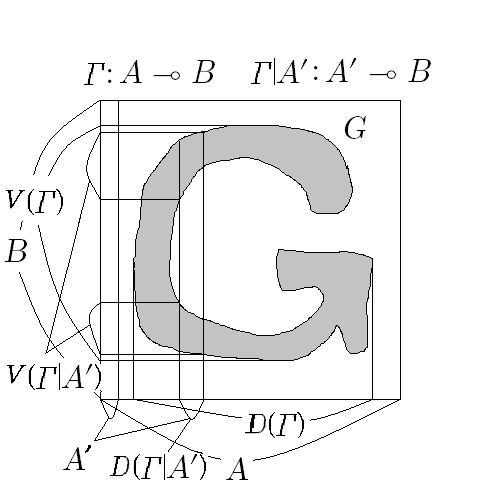
\includegraphics[width=160pt]{1.2.1.a.png}
\end{center}
2つの対応たち$\varGamma:A \multimap B$、$\varDelta:A \multimap B$が与えられたとき、これらの対応たちが等しいかどうかの判定法として、定理\ref{1.2.1.17}が知られており、$\forall a \in A$に対し、$\varGamma\left( \left\{ a \right\} \right) = \varDelta\left( \left\{ a \right\} \right)$が成り立つならそのときに限り、$\varGamma:A \multimap B = \varDelta:A \multimap B$が成り立つことを主張しているのであった。
\begin{thm}
\label{1.2.2.6}
次のことが成り立つ。
\begin{itemize}
\item
  2つの集合たち$A$、$B$の直積$A \times B$とこれの部分集合$G$が与えられれば、対応$\varGamma:A \multimap B = (A \times B,G)$が一意的に決まる。
\item
  1つの対応$\varGamma:A \multimap B$について$A'\in \mathfrak{P}(A)$なる集合$A'$を用いて$V\left( \varGamma|A' \right) = \bigcup_{a \in A'} {V\left( \varGamma|\left\{ a \right\} \right)}$が成り立つ。
\end{itemize}
\end{thm}
\begin{proof}
2つの集合たち$A$、$B$の直積$A \times B$とこれの部分集合$G$が与えられたとき、直積$A \times B$は一意的に存在するかつ、集合$\left\{ \left\{ A \times B \right\},\left\{ A \times B,G \right\} \right\}$も一意的に存在するので、順序対$(A \times B,G)$も一意的に存在する。対応の定義より、よって、対応$\varGamma:A \multimap B = (A \times B,G)$が一意的に決まる。\par
1つの対応$\varGamma:A \multimap B$について$A'\in \mathfrak{P}(A)$なる集合$A'$を用いて次のようになる。
\begin{align*}
V\left( \varGamma|A' \right) &= \left\{ b \in B \middle| \exists a \in A'\left[ (a,b) \in G \right] \right\}\\
&= \bigcup_{a \in A'} \left\{ b \in B \middle| (a,b) \in G \right\}\\
&= \bigcup_{a \in A'} \left\{ b \in B \middle| \exists a \in \left\{ a \right\}\left[ (a,b) \in G \right] \right\}\\
&= \bigcup_{a \in A'} {V\left( \varGamma\left| \text{\{}a \right\} \right)}
\end{align*}
\end{proof}
対応$\varGamma:A \multimap B = (A \times B,G)$において、$\forall(a,b) \in A \times B$に対し、$(a,b) \in G \Leftrightarrow (b,a) \in H$となるような対応$(B \times A,H)$も考えられることができ、これをその対応$\varGamma:A \multimap B$の逆対応といい$\varGamma^{- 1}:B \multimap A$と書くのであった。ここで、その対応$\varGamma^{- 1}$によるその集合$B$の部分集合$B'$の像$V\left( \varGamma^{- 1}|B' \right)$をその対応$\varGamma$によるその集合$B'$の原像、逆像などという。\par
対応$\varGamma:A \multimap B = (A \times B,G)$の逆対応$\varGamma^{- 1}$が$\varGamma^{- 1}:B \multimap A = (B \times A,H)$と与えられたとき、これのgraph$H$については定理\ref{1.2.1.18}より$H = \left\{ (b,a) \in B \times A \middle| (a,b) \in G \right\}$が成り立つのであった。
\begin{thm}
\label{1.2.2.7}
対応$\varGamma:A \multimap B = (A \times B,G)$において、次式たちが成り立つ。
\begin{align*}
\left( \varGamma^{- 1} \right)^{- 1} &= \varGamma\\
D\left( \varGamma^{- 1} \right) &= V(\varGamma)\\
V\left( \varGamma^{- 1} \right) &= D(\varGamma)\\
\left( \varGamma^{- 1} \right)^{- 1}:A \multimap B &= (A \times B,G) = \varGamma:A \multimap B
\end{align*}
\end{thm}
\begin{proof}
対応$\varGamma:A \multimap B = (A \times B,G)$において、これの逆対応$\varGamma^{-1} $のgraphを$H$、これの逆対応$\left( \varGamma^{-1} \right)^{-1} $のgraphを$I$とおくと、$\forall (a,b) \in A\times B$に対し、定理\ref{1.2.1.18}より次のようになることから、
\begin{align*}
(a,b)\in G \Leftrightarrow (a,b) \in H \Leftrightarrow (a,b) \in I
\end{align*}
外延性の公理より$G=I$が成り立ち、対応の定義よりよって、$\left( \varGamma^{- 1} \right)^{- 1} = \varGamma$が成り立つ。\par
$\forall b \in D\left( \varGamma^{- 1} \right)$に対し、次のようになる。
\begin{align*}
b \in D\left( \varGamma^{- 1} \right) &\Leftrightarrow b \in \left\{ b \in B \middle| V\left( \varGamma^{- 1} \right) \neq \emptyset \right\}\\
&\Leftrightarrow b \in B \land V\left( \varGamma^{- 1} \right) \neq \emptyset\\
&\Leftrightarrow b \in B \land \neg\left( \left\{ a \in A \middle| \exists b \in B\left[ (b,a) \in G' \right] \right\} = \emptyset \right)\\
&\Leftrightarrow b \in B \land \neg\left( \left\{ a \in A \middle| \exists b \in B\left[ (a,b) \in G \right] \right\} = \left\{ a \in A \middle| \bot \right\} \right)
\end{align*}
外延性の公理より$\forall a \in A$に対し、次のようになる。
\begin{align*}
&\quad \left( a \in \left\{ a \in A \middle| \exists b \in B\left[ (a,b) \in G \right] \right\} \Leftrightarrow a \in \left\{ a \in A \middle| \bot \right\} \right)\\
&\Leftrightarrow \left( a \in A \land \exists b \in B\left[ (a,b) \in G \right] \Leftrightarrow a \in A \land \bot \right)\\
&\Leftrightarrow \left( a \in A \land \exists b \in B\left[ (a,b) \in G \right] \Leftrightarrow \bot \right)\\
&\Leftrightarrow \neg\left( \left( a \in A \land \exists b \in B\left[ (a,b) \in G \right] \right) \vee \bot \right) \\
&\quad \vee \left( a \in A \land \exists b \in B\left[ (a,b) \in G \right] \land \bot \right)\\
&\Leftrightarrow \neg\left( a \in A \land \exists b \in B\left[ (a,b) \in G \right] \right) \vee \bot\\
&\Leftrightarrow \neg\left( a \in A \land \exists b \in B\left[ (a,b) \in G \right] \right)
\end{align*}
以上より、次のようになる。
\begin{align*}
b \in D\left( \varGamma^{- 1} \right) &\Leftrightarrow b \in B \land \neg\forall a \in A\left[ \neg\left( a \in A \land \exists b \in B\left[ (a,b) \in G \right] \right) \right]\\
&\Leftrightarrow b \in B \land \exists a \in A\left[ a \in A \land \exists b \in B\left[ (a,b) \in G \right] \right]\\
&\Leftrightarrow b \in B \land \exists a \in A\exists b \in B\left[ (a,b) \in G \right]\\
&\Leftrightarrow \exists b \in B\left[ b \in B \land \exists a \in A\left[ (a,b) \in G \right] \right]\\
&\Leftrightarrow \exists b \in B\exists a \in A\left[ (a,b) \in G \right]\\
&\Leftrightarrow b \in B \land \exists a \in A\left[ (a,b) \in G \right]\\
&\Leftrightarrow b \in \left\{ b \in B \middle| \exists a \in A\left[ (a,b) \in G \right] \right\}\\
&\Leftrightarrow b \in V(\varGamma)
\end{align*}
外延性の公理より、よって、$D\left( \varGamma^{- 1} \right) = V(\varGamma)$が成り立つ。\par
$\left( \varGamma^{- 1} \right)^{- 1} = \varGamma$と$D\left( \varGamma^{- 1} \right) = V(\varGamma)$が成り立つのであったので、$D\left( \left( \varGamma^{- 1} \right)^{- 1} \right) = V\left( \varGamma^{- 1} \right)$も成り立つ。よって、$V\left( \varGamma^{- 1} \right) = D(\varGamma)$が成り立つ。
\end{proof}
%\hypertarget{ux5199ux50cf}{%
\subsubsection{写像}%\label{ux5199ux50cf}}
対応$f:A \multimap B$について、$\forall a \in A\exists b \in B$に対し、$V\left( f|\left\{ a \right\} \right) = \left\{ b \right\}$が成り立つとき、その対応$f$を写像といい$f:A \rightarrow B$、$A\overset{f}{\rightarrow}B$などと書く。この写像$f:A \rightarrow B$全体の集合を$\mathfrak{F}(A,B)$、$B^{A}$などと書く。このとき、$V\left( f|\left\{ a \right\} \right) = \left\{ b \right\}$のことを、単に、$f(a) = b$と書き、これを明示するとき、その写像$f$を$f:A \rightarrow B;a \mapsto f(a) = b$などと書くときがありその元$b$をその元$a$のその写像$f$による像、その元$a$におけるその写像$f$の値などといいこのことをその写像$f$はその元$a$をその元$b$に写す、その元$a$にその元$b$を対応させるなどという。\par
これらの用語たちは次の図のように該当される。
\begin{center}
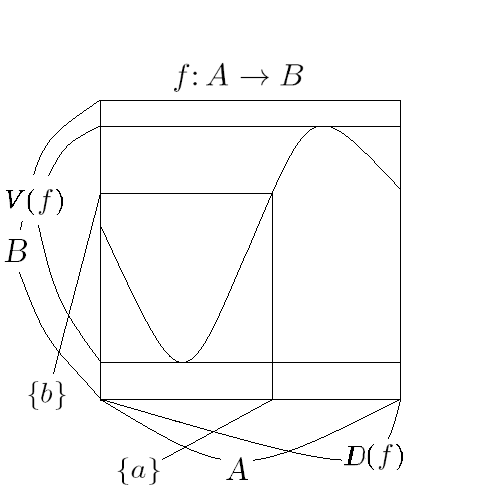
\includegraphics[width=160pt]{1.2.1.b.png}
\end{center}
\begin{thm}
\label{1.2.2.8}
対応$\varGamma:A \multimap B$と写像$f:A \rightarrow B$について、$A',A''\in \mathfrak{P}(A)$、$B',B''\in \mathfrak{P}(B)$なる集合たち$A'$、$A''$、$B'$、$B''$を用いると、次式が成り立つ。
\begin{align*}
A' \subseteq A'' &\Rightarrow V\left( \varGamma|A' \right) \subseteq V\left( \varGamma|A'' \right)\\
V\left( \varGamma|A' \cup A'' \right) &= V\left( \varGamma|A' \right) \cup V\left( \varGamma|A'' \right)\\
V\left( \varGamma|A' \cap A'' \right) &\subseteq V\left( \varGamma|A' \right) \cap V\left( \varGamma|A'' \right)\\
V\left( f^{- 1}|B' \cap B'' \right) &= V\left( f^{- 1}|B' \right) \cap V\left( f^{- 1}|B'' \right)\\
V\left( \varGamma|A \setminus A' \right) &\supseteq V\left( \varGamma|A \right) \setminus V\left( \varGamma|A' \right)\\
V\left( f^{- 1}|B \setminus B' \right) &= A \setminus V\left( f^{- 1}|B' \right)\\
V\left( f^{- 1}|V\left( f|A' \right) \right) &\supseteq A'\\
V\left( f|V\left( f^{- 1}|B' \right) \right) &\subseteq B'
\end{align*}
\end{thm}
\begin{proof}
対応$\varGamma:A \multimap B$について、$A',A''\in \mathfrak{P}(A)$、$B',B''\in \mathfrak{P}(B)$なる集合たち$A'$、$A''$、$B'$、$B''$を用いその対応$\varGamma$のgraphを$G$、これの逆対応のgraphを$G'$、その集合$A$の元の1つを$\overline{a}$、その集合$B$の元々2つを$\overline{b}$、$\overline{\overline{b}}$とする。このとき、$A' \subseteq A''$が成り立つなら、次のようになる。
\begin{align*}
b \in V\left( \varGamma|A' \right) &\Leftrightarrow b \in B \land \exists a \in A'\left[ (a,b) \in G \right]\\
&\Leftrightarrow b \in B \land \exists a \in A' \subseteq A''\left[ (a,b) \in G \right]\\
&\Rightarrow b \in B \land \exists a \in A''\left[ (a,b) \in G \right] \\
&\Leftrightarrow b \in V\left( \varGamma|A'' \right)
\end{align*}
したがって、$V\left( \varGamma|A' \right) \subseteq V\left( \varGamma|A'' \right)$が成り立ち、よって、次式が成り立つ。
\begin{align*}
A' \subseteq A'' \Rightarrow V\left( \varGamma|A' \right) \subseteq V\left( \varGamma|A'' \right)
\end{align*}\par
また、次のようになる。
\begin{align*}
b \in V\left( \varGamma|A' \cup A'' \right) &\Leftrightarrow b \in B \land \exists a \in A' \cup A''\left[ (a,b) \in G \right]\\
&\Leftrightarrow b \in B \land \overline{a} \in A' \cup A'' \land \left( \overline{a},b \right) \in G\\
&\Leftrightarrow b \in B \land \left( \overline{a} \in A' \vee \overline{a} \in A'' \right) \land \left( \overline{a},b \right) \in G\\
&\Leftrightarrow \left( b \in B \land \overline{a} \in A' \land \left( \overline{a},b \right) \in G \right) \\
&\quad \vee \left( b \in B \land \overline{a} \in A' \land \left( \overline{a},b \right) \in G \right)\\
&\Leftrightarrow \left( b \in B \land \exists a \in A'\left[ (a,b) \in G \right] \right) \\ 
&\quad \vee \left( b \in B \land \exists a \in A''\left[ (a,b) \in G \right] \right)\\
&\Leftrightarrow b \in V\left( \varGamma|A' \right) \vee b \in V\left( \varGamma|A'' \right) \\
&\Leftrightarrow b \in V\left( \varGamma|A' \right) \cup V\left( \varGamma|A'' \right)
\end{align*}
よって、次式が成り立つ。
\begin{align*}
V\left( \varGamma|A' \cup A'' \right) = V\left( \varGamma|A' \right) \cup V\left( \varGamma|A'' \right)
\end{align*}\par
また、次のようになる。
\begin{align*}
b \in V\left( \varGamma|A' \cap A'' \right) &\Leftrightarrow b \in B \land \exists a \in A' \cap A''\left[ (a,b) \in G \right]\\
&\Leftrightarrow b \in B \land \overline{a} \in A' \cap A'' \land \left( \overline{a},b \right) \in G\\
&\Leftrightarrow b \in B \land b \in B \land \overline{a} \in A' \land \overline{a} \in A'' \\
&\quad \land \left( \overline{a},b \right) \in G \land \left( \overline{a},b \right) \in G\\
&\Rightarrow b \in B \land \exists\overline{a} \in A'\left[ \left( \overline{a},b \right) \in G \right] \\
&\quad \land b \in B \land \exists\overline{a} \in A''\left[ \left( \overline{a},b \right) \in G \right]\\
&\Leftrightarrow b \in V\left( \varGamma|A' \right) \land b \in V\left( \varGamma|A'' \right) \\
&\Leftrightarrow b \in V\left( \varGamma|A' \right) \cap V\left( \varGamma|A'' \right)
\end{align*}
よって、次式が成り立つ。
\begin{align*}
V\left( \varGamma|A' \cap A'' \right) \subseteq V\left( \varGamma|A' \right) \cap V\left( \varGamma|A'' \right)
\end{align*}\par
また、次のようになる。
\begin{align*}
a \in V\left( f^{- 1}|B' \right) \cap V\left( f^{- 1}|B'' \right) &\Leftrightarrow a \in V\left( f^{- 1}|B' \right) \land a \in V\left( f^{- 1}|B'' \right)\\
&\Leftrightarrow \left( a \in A \land \exists b \in B'\left[ (a,b) \in G \right] \right) \\
&\quad \land \left( a \in A \land \exists b \in B''\left[ (a,b) \in G \right] \right)\\
&\Leftrightarrow a \in A \land \exists b \in B'\left[ (a,b) \in G \right] \land \exists b \in B''\left[ (a,b) \in G \right]\\
&\Leftrightarrow a \in A \land \overline{b} \in B' \land \left( a,\overline{b} \right) \in G \land \overline{\overline{b}} \in B'' \land \left( a,\overline{\overline{b}} \right) \in G\\
&\Leftrightarrow a \in A \land \overline{b} \in B' \land a \in \left\{ a \right\} \land \left( a,\overline{b} \right) \in G \\
&\quad \land \overline{\overline{b}} \in B'' \land a \in \left\{ a \right\} \land \left( a,\overline{\overline{b}} \right) \in G\\
&\Leftrightarrow a \in A \land \overline{b} \in \left\{ \overline{b} \in B' \middle| \exists a \in \left\{ a \right\}\left[ \left( a,\overline{b} \right) \in G \right] \right\} \\
&\quad \land \overline{\overline{b}} \in \left\{ \overline{\overline{b}} \in B'' \middle| \exists a \in \left\{ a \right\}\left[ \left( a,\overline{\overline{b}} \right) \in G \right] \right\}\\
&\Leftrightarrow \forall a \in A\left[ \overline{b} \in V\left( f|\left\{ a \right\} \right) \subseteq B' \land \overline{\overline{b}} \in V\left( f|\left\{ a \right\} \right) \subseteq B'' \right]
\end{align*}
ここで、その対応$f$は写像なので、$\forall a \in A$に対し、$V\left( f|\left\{ a \right\} \right) = \left\{ b \right\}$が成り立つ。したがって、次のようになる。
\begin{align*}
a \in V\left( f^{- 1}|B' \right) \cap V\left( f^{- 1}|B'' \right) &\Leftrightarrow \forall a \in A\left[ \overline{b} \in \left\{ b \right\} \land \overline{\overline{b}} \in \left\{ b \right\} \right]\\
&\Leftrightarrow \forall a \in A\left[ b = \overline{b} = \overline{\overline{b}} \right]
\end{align*}
これにより、$b = \overline{b} = \overline{\overline{b}}$が成り立つので、次のようになる。
\begin{align*}
a \in V\left( f^{- 1}|B' \right) \cap V\left( f^{- 1}|B'' \right) &\Leftrightarrow a \in A \land \overline{b} \in B' \land \left( a,\overline{b} \right) \in G \land \overline{\overline{b}} \in B'' \land \left( a,\overline{\overline{b}} \right) \in G\\
&\Rightarrow a \in A \land \overline{b} \in B' \land \overline{b} \in B'' \land \left( a,\overline{b} \right) \in G\\
&\Leftrightarrow a \in A \land \overline{b} \in B' \cap B'' \land \left( a,\overline{b} \right) \in G\\
&\Leftrightarrow a \in A \land \exists b \in B' \cap B''\left[ (a,b) \in G \right]\\
&\Leftrightarrow a \in \left\{ a \in A \middle| \exists b \in B' \cap B''\left[ (a,b) \in G \right] \right\}\\
&\Leftrightarrow a \in V\left( f^{- 1}|B' \cap B'' \right)
\end{align*}
これにより、$V\left( f^{- 1}|B' \right) \cap V\left( f^{- 1}|B'' \right) \subseteq V\left( f^{- 1}|B' \cap B'' \right)$が得られた。ここで、上記の議論により$V\left( f^{- 1}|B' \cap B'' \right) \subseteq V\left( f^{- 1}|B' \right) \cap V\left( f^{- 1}|B'' \right)$が成り立つのであったので、次式が成り立つ。
\begin{align*}
V\left( f^{- 1}|B' \cap B'' \right) = V\left( f^{- 1}|B' \right) \cap V\left( f^{- 1}|B'' \right)
\end{align*}\par
また、次のようになる。
\begin{align*}
b \in V\left( \varGamma|A \right) \setminus V\left( \varGamma|A' \right) &\Leftrightarrow b \in V\left( \varGamma|A \setminus A' \cup A' \right) \setminus V\left( \varGamma|A' \right)\\
&\Leftrightarrow b \in \left( V\left( \varGamma|A \setminus A' \right) \cup V\left( \varGamma|A' \right) \right) \setminus V\left( \varGamma|A' \right)\\
&\Leftrightarrow b \in \left( V\left( \varGamma|A \setminus A' \right) \setminus V\left( \varGamma|A' \right) \right) \\
&\quad \cup \left( V\left( \varGamma|A' \right) \setminus V\left( \varGamma|A' \right) \right)\\
&\Leftrightarrow b \in \left( V\left( \varGamma|A \setminus A' \right) \setminus V\left( \varGamma|A' \right) \right) \cup \emptyset\\
&\Leftrightarrow b \in V\left( \varGamma|A \setminus A' \right) \setminus V\left( \varGamma|A' \right)\\
&\Leftrightarrow b \in V\left( \varGamma|A \setminus A' \right) \cap b \notin V\left( \varGamma|A' \right)\\
&\Rightarrow b \in V\left( \varGamma|A \setminus A' \right)
\end{align*}
よって、次式が成り立つ。
\begin{align*}
V\left( \varGamma|A \setminus A' \right) \supseteq V\left( \varGamma|A \right) \setminus V\left( \varGamma|A' \right)
\end{align*}\par
また、明らかに$B \setminus B' \subseteq B$が成り立つので、次のようになる。
\begin{align*}
a \in V\left( f^{- 1}|B \setminus B' \right) &\Leftrightarrow a \in V\left( f^{- 1}|B \cap \left( B \setminus B' \right) \right)\\
&\Leftrightarrow a \in V\left( f^{- 1}|B \right) \cap V\left( f^{- 1}|B \setminus B' \right)\\
&\Leftrightarrow a \in V\left( f^{- 1}|B \right) \land a \in V\left( f^{- 1}|B \setminus B' \right)
\end{align*}
ここで、$a \in V\left( f^{- 1}|B \setminus B' \right) \cap V\left( f^{- 1}|B' \right)$が成り立つと仮定しよう。このとき、次のようになる。
\begin{align*}
a \in V\left( f^{- 1}|B \setminus B' \right) \cap V\left( f^{- 1}|B' \right) &\Leftrightarrow a \in V\left( f^{- 1}|B \setminus B' \right) \land a \in V\left( f^{- 1}|B' \right)\\
&\Leftrightarrow a \in A \land \exists b \in B \setminus B'\left[ (a,b) \in G \right] \land \exists b \in B'\left[ (a,b) \in G \right]\\
&\Leftrightarrow a \in A \land \overline{b} \in B \setminus B' \land \left( a,\overline{b} \right) \in G \land \overline{\overline{b}} \in B' \land \left( a,\overline{\overline{b}} \right) \in G\\
&\Leftrightarrow a \in A \land \overline{b} \in B \setminus B' \land a \in \left\{ a \right\} \land \left( a,\overline{b} \right) \in G \\
&\quad \land \overline{\overline{b}} \in B' \land a \in \left\{ a \right\} \land \left( a,\overline{\overline{b}} \right) \in G\\
&\Leftrightarrow a \in A \land \overline{b} \in \left\{ \overline{b} \in B \setminus B' \middle| \exists a \in \left\{ a \right\}\left[ \left( a,\overline{b} \right) \in G \right] \right\} \\
&\quad \land \overline{\overline{b}} \in \left\{ \overline{\overline{b}} \in B' \middle| \exists a \in \left\{ a \right\}\left[ \left( a,\overline{\overline{b}} \right) \in G \right] \right\}\\
&\Leftrightarrow \forall a \in A\left[ \overline{b} \in V\left( f|\left\{ a \right\} \right) \subseteq B \setminus B' \land \overline{\overline{b}} \in V\left( f|\left\{ a \right\} \right) \subseteq B' \right]
\end{align*}
ここで、その対応$f$は写像なので、$\forall a \in A$に対し、$V\left( f|\left\{ a \right\} \right) = \left\{ b \right\}$が成り立つ。したがって、次のようになる。
\begin{align*}
a \in V\left( f^{- 1}|B \setminus B' \right) \cap V\left( f^{- 1}|B' \right) &\Leftrightarrow \forall a \in A\left[ \overline{b} \in \left\{ b \right\} \land \overline{\overline{b}} \in \left\{ b \right\} \right]\\
&\Leftrightarrow \forall a \in A\left[ b = \overline{b} = \overline{\overline{b}} \right]
\end{align*}
これにより、$b = \overline{b} = \overline{\overline{b}}$が成り立つので、次のようになる。
\begin{align*}
a \in V\left( f^{- 1}|B \setminus B' \right) \cap V\left( f^{- 1}|B' \right) &\Leftrightarrow a \in A \land \overline{b} \in B \setminus B' \land \left( a,\overline{b} \right) \in G \land \overline{\overline{b}} \in B' \land \left( a,\overline{\overline{b}} \right) \in G\\
&\Rightarrow a \in A \land \overline{b} \in B \setminus B' \land \overline{b} \in B' \land \left( a,\overline{b} \right) \in G\\
&\Leftrightarrow a \in A \land \overline{b} \in B \land \overline{b} \notin B' \land \overline{b} \in B' \land \left( a,\overline{b} \right) \in G\\
&\Leftrightarrow a \in A \land \overline{b} \in B \land \bot \land \left( a,\overline{b} \right) \in G \Leftrightarrow \bot
\end{align*}
これは矛盾しているので、$a \in V\left( f^{- 1}|B \setminus B' \right) \cap V\left( f^{- 1}|B' \right)$が成り立たないことになる。したがって、$a \in V\left( f^{- 1}|B \setminus B' \right) \Rightarrow a \notin V\left( f^{- 1}|B' \right)$が成り立つ。\par
これにより、次のようになる。
\begin{align*}
a \in V\left( f^{- 1}|B \setminus B' \right) &\Leftrightarrow a \in V\left( f^{- 1}|B \right) \land a \in V\left( f^{- 1}|B \setminus B' \right)\\
&\Rightarrow a \in V\left( f^{- 1}|B \right) \land a \notin V\left( f^{- 1}|B' \right)\\
&\Leftrightarrow a \in V\left( f^{- 1}|B \right) \setminus V\left( f^{- 1}|B' \right)
\end{align*}\par
また、次のようになることから
\begin{align*}
a \in A' &\Rightarrow a \in A \land f(a) \in V\left( f|A' \right)\\
&\Rightarrow a \in A \land \exists b \in V\left( f|A' \right)\left[ b = f(a) \right]\\
&\Rightarrow a \in V\left( f^{- 1}|V\left( f|A' \right) \right)
\end{align*}
次式が得られる。
\begin{align*}
V\left( f^{- 1}|V\left( f|A' \right) \right) \supseteq A'
\end{align*}\par
また、次のようになることから
\begin{align*}
b \in V\left( f|V\left( f^{- 1}|B' \right) \right) &\Leftrightarrow b \in B \land \exists a \in V\left( f^{- 1}|B' \right)\left[ b = f(a) \right]\\
&\Leftrightarrow b \in B \land \overline{a} \in V\left( f^{- 1}|B' \right) \land f\left( \overline{a} \right) = b\\
&\Leftrightarrow b \in B \land \overline{a} \in A \land \exists b' \in B'\left[ f\left( \overline{a} \right) = b' \right] \land f\left( \overline{a} \right) = b\\
&\Leftrightarrow b \in B \land \overline{a} \in A \land \overline{b'} \in B' \land f\left( \overline{a} \right) = \overline{b'} \land f\left( \overline{a} \right) = b\\
&\Rightarrow b \in B \land \overline{b'} \in B' \land b = \overline{b'} \Rightarrow b \in B'
\end{align*}
次式が得られる。
\begin{align*}
V\left( f|V\left( f^{- 1}|B' \right) \right) \subseteq B'
\end{align*}
\end{proof}
\begin{thm}
\label{1.2.2.9}
対応$\varGamma:A \multimap B$と写像$f:A \rightarrow B$について、$\mathcal{A \in}\mathfrak{P}\left( \mathfrak{P}(A) \right)$なる集合$\mathcal{A}$と$\mathcal{B \in}\mathfrak{P}\left( \mathfrak{P}(B) \right)$なる集合$\mathcal{B}$に対し、次式が成り立つ。
\begin{align*}
V\left( \varGamma|\bigcup_{A \in \mathcal{A}} A \right) &= \bigcup_{A \in \mathcal{A}} {V\left( \varGamma|A \right)}\\
V\left( \varGamma|\bigcap_{A \in \mathcal{A}} A \right) &\subseteq \bigcap_{A \in \mathcal{A}} {V\left( \varGamma|A \right)}\\
V\left( f^{- 1}|\bigcap_{B\in \mathcal{B}} B \right) &= \bigcap_{B\in \mathcal{B}} {V\left( f^{- 1}|B \right)}
\end{align*}
\end{thm}
\begin{proof}
対応$\varGamma:A \multimap B$と写像$f:A \rightarrow B$について、$\mathcal{A}\in \mathfrak{P}\left( \mathfrak{P}(A) \right)$なる集合$\mathcal{A}$と$\mathcal{B}\in \mathfrak{P}\left( \mathfrak{P}(B) \right)$なる集合$\mathcal{B}$が与えられたとする。$\forall a \in V\left( \varGamma|\bigcup_{A \in \mathcal{A}} A \right)$に対し、次のようになる。
\begin{align*}
b \in V\left( \varGamma|\bigcup_{A \in \mathcal{A}} A \right)\bigcup_{A \in \mathcal{A}} {V\left( \varGamma|A \right)} &\Leftrightarrow b \in B \land \exists a \in \bigcup_{A \in \mathcal{A}} A\left[ (a,b) \in G \right]\\
&\Leftrightarrow b \in B \land \overline{a} \in \bigcup_{A \in \mathcal{A}} A \land \left( \overline{a},b \right) \in G\\
&\Leftrightarrow b \in B \land \exists A \in \mathcal{A}\left[ \overline{a} \in A \right] \land \left( \overline{a},b \right) \in G\\
&\Leftrightarrow \exists A \in \mathcal{A}\left[ b \in B \land \overline{a} \in A \land \left( \overline{a},b \right) \in G \right]\\
&\Leftrightarrow \exists A \in \mathcal{A}\left[ b \in B \land \exists a \in A\left[ (a,b) \in G \right] \right]\\
&\Leftrightarrow \exists A \in \mathcal{A}\left[ b \in V\left( \varGamma|A \right) \right] \vee b \in V\left( \varGamma|A'' \right)\\
&\Leftrightarrow b \in \bigcup_{A \in \mathcal{A}} {V\left( \varGamma|A \right)}
\end{align*}
よって、次式が成り立つ。
\begin{align*}
V\left( \varGamma|\bigcup_{A \in \mathcal{A}} A \right) = \bigcup_{A \in \mathcal{A}} {V\left( \varGamma|A \right)}
\end{align*}\par
$\forall a \in V\left( \varGamma|\bigcap_{A \in \mathcal{A}} A \right)$に対し、次のようになる。
\begin{align*}
b \in V\left( \varGamma|\bigcap_{A \in \mathcal{A}} A \right) &\Leftrightarrow b \in B \land \exists a \in \bigcap_{A \in \mathcal{A}} A\left[ (a,b) \in G \right]\\
&\Leftrightarrow b \in B \land \overline{a} \in \bigcap_{A \in \mathcal{A}} A \land \left( \overline{a},b \right) \in G\\
&\Leftrightarrow b \in B \land \forall A \in \mathcal{A}\left[ \overline{a} \in A \right] \land \left( \overline{a},b \right) \in G\\
&\Rightarrow \forall A \in \mathcal{A}\left[ b \in B \land \exists\overline{a} \in A\left[ \left( \overline{a},b \right) \in G \right] \right]\\
&\Leftrightarrow \forall A \in \mathcal{A}\left[ b \in V\left( \varGamma|A' \right) \land b \in V\left( \varGamma|A'' \right) \right]\\
&\Leftrightarrow b \in \bigcap_{A \in \mathcal{A}} {V\left( \varGamma|A \right)}
\end{align*}
よって、次式が成り立つ。
\begin{align*}
V\left( \varGamma|\bigcap_{A \in \mathcal{A}} A \right) \subseteq \bigcap_{A \in \mathcal{A}} {V\left( \varGamma|A \right)}
\end{align*}\par 
$\forall a \in \bigcap_{B\in \mathcal{B}} {V\left( f^{- 1}|B \right)} $に対し、次のようになる。
\begin{align*}
a \in \bigcap_{B\in \mathcal{B}} {V\left( f^{- 1}|B \right)} &\Leftrightarrow \forall B\in \mathcal{B}\left[ a \in V\left( f^{- 1}|B \right) \right]\\
&\Leftrightarrow \forall B\in \mathcal{B}\left[ a \in A \land \exists b \in B\left[ (a,b) \in G \right] \right]\\
&\Leftrightarrow a \in A \land \forall B\in \mathcal{B\exists}b \in B\left[ (a,b) \in G \right]\\
&\Leftrightarrow a \in A \land \forall B\in \mathcal{B}\left[ {\overline{b}}_{B} \in B \land \left( a,{\overline{b}}_{B} \right) \in G \right]\\
&\Leftrightarrow a \in A \land \forall B\in \mathcal{B}\left[ {\overline{b}}_{B} \in B \land a \in \left\{ a \right\} \land \left( a,{\overline{b}}_{B} \right) \in G \right]\\
&\Leftrightarrow a \in A \land \forall B\in \mathcal{B}\left[ {\overline{b}}_{B} \in \left\{ {\overline{b}}_{B} \in B' \middle| \exists a \in \left\{ a \right\}\left[ \left( a,{\overline{b}}_{B} \right) \in G \right] \right\} \right]\\
&\Leftrightarrow \forall a \in A\forall B\in \mathcal{B}\left[ {\overline{b}}_{B} \in V\left( f|\left\{ a \right\} \right) \subseteq B \right]
\end{align*}
ここで、その対応$f$は写像なので、$\forall a \in A$に対し、$V\left( f|\left\{ a \right\} \right) = \left\{ \overline{b} \right\}$が成り立つ。したがって、次のようになる。
\begin{align*}
a \in \bigcap_{B\in \mathcal{B}} {V\left( f^{- 1}|B \right)} &\Leftrightarrow \forall a \in A\forall B\in \mathcal{B}\left[ {\overline{b}}_{B} \in \left\{ \overline{b} \right\} \right]\\
&\Leftrightarrow \forall a \in A\forall B\in \mathcal{B}\left[ \overline{b} = {\overline{b}}_{B} \right]
\end{align*}
これにより、$\forall B\in \mathcal{B}$に対し、$\overline{b} = {\overline{b}}_{B}$が成り立つので、次のようになる。
\begin{align*}
a \in \bigcap_{B\in \mathcal{B}} {V\left( f^{- 1}|B \right)} &\Leftrightarrow \forall a \in A\forall B\in \mathcal{B}\left[ {\overline{b}}_{B} \in V\left( f|\left\{ a \right\} \right) \subseteq B \right]\\
&\Rightarrow \forall a \in A\forall B\in \mathcal{B}\left[ \overline{b} \in V\left( f|\left\{ a \right\} \right) \subseteq B \right]\\
&\Leftrightarrow a \in A \land \forall B\in \mathcal{B}\left[ \overline{b} \in B \land \left( a,\overline{b} \right) \in G \right]\\
&\Leftrightarrow a \in A \land \forall B\in \mathcal{B}\left[ \overline{b} \in B \right] \land \left( a,\overline{b} \right) \in G\\
&\Leftrightarrow a \in A \land \overline{b} \in \bigcap_{B\in \mathcal{B}} B \land \left( a,\overline{b} \right) \in G\\
&\Leftrightarrow a \in A \land \exists b \in \bigcap_{B\in \mathcal{B}} B\left[ (a,b) \in G \right]\\
&\Leftrightarrow a \in \left\{ a \in A \middle| \exists b \in \bigcap_{B\in \mathcal{B}} B\left[ (a,b) \in G \right] \right\}\\
&\Leftrightarrow a \in V\left( f^{- 1}|\bigcap_{B\in \mathcal{B}} B \right)
\end{align*}
これにより、$\bigcap_{B\in \mathcal{B}} {V\left( f^{- 1}|B \right)} \subseteq V\left( f^{- 1}|\bigcap_{B\in \mathcal{B}} B \right)$が得られた。ここで、上記の議論により$V\left( f^{- 1}|\bigcap_{B\in \mathcal{B}} B \right) \subseteq \bigcap_{B\in \mathcal{B}} {V\left( f^{- 1}|B \right)}$が成り立つのであったので、次式が成り立つ。
\begin{align*}
V\left( f^{- 1}|\bigcap_{B\in \mathcal{B}} B \right) = \bigcap_{B\in \mathcal{B}} {V\left( f^{- 1}|B \right)}
\end{align*}
\end{proof}
\begin{thebibliography}{50}
  \bibitem{1}
    Rei Frontier Tech Blog. "ZFC公理系について:その1". Hatena Blog. \url{https://tech-blog.rei-frontier.jp/entry/2017/11/02/102042}, (2021-04-01 20:30 閲覧)
  \bibitem{2}
    Rei Frontier Tech Blog. "ZFC公理系について:その2". Hatena Blog. \url{https://tech-blog.rei-frontier.jp/entry/2017/11/09/100000}, (2021-04-01 20:30 閲覧)
  \bibitem{3}
    Rei Frontier Tech Blog. "ZFC公理系について:その3". Hatena Blog. \url{https://tech-blog.rei-frontier.jp/entry/2017/11/16/100000} (2021-04-01 20:30 閲覧)
  \bibitem{4}
    松坂和夫, 集合・位相入門, 岩波書店, 1968. 新装版第2刷 p1-39 ISBM978-4-00-029871-1
\end{thebibliography}
\end{document}

\clearpage
\documentclass[dvipdfmx]{jsarticle}
\setcounter{section}{2}
\setcounter{subsection}{2}
\usepackage{xr}
\externaldocument{1.2.1}
\externaldocument{1.2.2}
\usepackage{amsmath,amsfonts,amssymb,array,comment,mathtools,url,docmute}
\usepackage{longtable,booktabs,dcolumn,tabularx,mathtools,multirow,colortbl,xcolor}
\usepackage[dvipdfmx]{graphics}
\usepackage{bmpsize}
\usepackage{amsthm}
\usepackage{enumitem}
\setlistdepth{20}
\renewlist{itemize}{itemize}{20}
\setlist[itemize]{label=•}
\renewlist{enumerate}{enumerate}{20}
\setlist[enumerate]{label=\arabic*.}
\setcounter{MaxMatrixCols}{20}
\setcounter{tocdepth}{3}
\newcommand{\rotin}{\text{\rotatebox[origin=c]{90}{$\in $}}}
\newcommand{\amap}[6]{\text{\raisebox{-0.7cm}{\begin{tikzpicture} 
  \node (a) at (0, 1) {$\textstyle{#2}$};
  \node (b) at (#6, 1) {$\textstyle{#3}$};
  \node (c) at (0, 0) {$\textstyle{#4}$};
  \node (d) at (#6, 0) {$\textstyle{#5}$};
  \node (x) at (0, 0.5) {$\rotin $};
  \node (x) at (#6, 0.5) {$\rotin $};
  \draw[->] (a) to node[xshift=0pt, yshift=7pt] {$\textstyle{\scriptstyle{#1}}$} (b);
  \draw[|->] (c) to node[xshift=0pt, yshift=7pt] {$\textstyle{\scriptstyle{#1}}$} (d);
\end{tikzpicture}}}}
\newcommand{\twomaps}[9]{\text{\raisebox{-0.7cm}{\begin{tikzpicture} 
  \node (a) at (0, 1) {$\textstyle{#3}$};
  \node (b) at (#9, 1) {$\textstyle{#4}$};
  \node (c) at (#9+#9, 1) {$\textstyle{#5}$};
  \node (d) at (0, 0) {$\textstyle{#6}$};
  \node (e) at (#9, 0) {$\textstyle{#7}$};
  \node (f) at (#9+#9, 0) {$\textstyle{#8}$};
  \node (x) at (0, 0.5) {$\rotin $};
  \node (x) at (#9, 0.5) {$\rotin $};
  \node (x) at (#9+#9, 0.5) {$\rotin $};
  \draw[->] (a) to node[xshift=0pt, yshift=7pt] {$\textstyle{\scriptstyle{#1}}$} (b);
  \draw[|->] (d) to node[xshift=0pt, yshift=7pt] {$\textstyle{\scriptstyle{#2}}$} (e);
  \draw[->] (b) to node[xshift=0pt, yshift=7pt] {$\textstyle{\scriptstyle{#1}}$} (c);
  \draw[|->] (e) to node[xshift=0pt, yshift=7pt] {$\textstyle{\scriptstyle{#2}}$} (f);
\end{tikzpicture}}}}
\renewcommand{\thesection}{第\arabic{section}部}
\renewcommand{\thesubsection}{\arabic{section}.\arabic{subsection}}
\renewcommand{\thesubsubsection}{\arabic{section}.\arabic{subsection}.\arabic{subsubsection}}
\everymath{\displaystyle}
\allowdisplaybreaks[4]
\usepackage{vtable}
\theoremstyle{definition}
\newtheorem{thm}{定理}[subsection]
\newtheorem*{thm*}{定理}
\newtheorem{dfn}{定義}[subsection]
\newtheorem*{dfn*}{定義}
\newtheorem{axs}[dfn]{公理}
\newtheorem*{axs*}{公理}
\renewcommand{\headfont}{\bfseries}
\makeatletter
  \renewcommand{\section}{%
    \@startsection{section}{1}{\z@}%
    {\Cvs}{\Cvs}%
    {\normalfont\huge\headfont\raggedright}}
\makeatother
\makeatletter
  \renewcommand{\subsection}{%
    \@startsection{subsection}{2}{\z@}%
    {0.5\Cvs}{0.5\Cvs}%
    {\normalfont\LARGE\headfont\raggedright}}
\makeatother
\makeatletter
  \renewcommand{\subsubsection}{%
    \@startsection{subsubsection}{3}{\z@}%
    {0.4\Cvs}{0.4\Cvs}%
    {\normalfont\Large\headfont\raggedright}}
\makeatother
\makeatletter
\renewenvironment{proof}[1][\proofname]{\par
  \pushQED{\qed}%
  \normalfont \topsep6\p@\@plus6\p@\relax
  \trivlist
  \item\relax
  {
  #1\@addpunct{.}}\hspace\labelsep\ignorespaces
}{%
  \popQED\endtrivlist\@endpefalse
}
\makeatother
\renewcommand{\proofname}{\textbf{証明}}
\usepackage{tikz,graphics}
\usepackage[dvipdfmx]{hyperref}
\usepackage{pxjahyper}
\hypersetup{
 setpagesize=false,
 bookmarks=true,
 bookmarksdepth=tocdepth,
 bookmarksnumbered=true,
 colorlinks=false,
 pdftitle={},
 pdfsubject={},
 pdfauthor={},
 pdfkeywords={}}
\begin{document}
%\hypertarget{ux5199ux50cf}{%
\subsection{写像}%\label{ux5199ux50cf}}
%\hypertarget{ux5bfeux5fdc}{%
\subsubsection{対応}%\label{ux5bfeux5fdc}}\par
復習のため対応に関する諸概念を再掲しておこう。\par
2つの集合たち$A$、$B$の直積$A \times B$とこれの部分集合$G$の順序対$(A \times B,G)$をその集合$A$からその集合$B$への対応といい、これを$\varGamma$とおくとき、$\varGamma:A \multimap B$と書くのであった。ここで、その集合$A$をその対応$\varGamma$の始集合、その集合$B$をその対応$\varGamma$の終集合、その集合$G$をその対応$\varGamma$のgraphという。対応$\varGamma:A \multimap B = (A \times B,G)$において、始集合$A$をこれの部分集合$A'$に変えた対応$\left( A' \times B,G \cap \left( A' \times B \right) \right)$をその対応$\varGamma$のその集合$A'$に制限したときの対応などといい$\varGamma|A'$などと書くのであった。\par
対応$\varGamma:A \multimap B = (A \times B,G)$において、$A'\in \mathfrak{P}(A)$なる集合$A'$を用いた集合$\left\{ b \in B \middle| \exists a \in A'\left[ (a,b) \in G \cap \left( A' \times B \right) \right] \right\}$をその集合$A'$のその対応$\varGamma$による像、その対応$\varGamma$をその集合$A'$に制限したときの対応$\varGamma|A'$の値域といい、$V\left( \varGamma|A' \right)$、$\varGamma\left( A' \right)$などと書く。特に、集合$\left\{ b \in B \middle| \exists a \in A\left[ (a,b) \in G \right] \right\}$を、単に、その対応$\varGamma$の値域といい、$V(\varGamma)$、$\varGamma(A)$などと書く。また、集合$\left\{ a \in A' \middle| V\left( \varGamma|A' \right) \neq \emptyset \right\}$をその対応$\varGamma$をその集合$A'$に制限したときの対応$\varGamma|A'$の定義域といい$D\left( \varGamma|A' \right)$などと書く。特に、集合$\left\{ a \in A \middle| V(\varGamma) \neq \emptyset \right\}$を、単に、その対応$\varGamma$の定義域といい、単に、$D(\varGamma)$などと書く。\par
以上のことが式で書かれれば、次のようになる。
\begin{longtable}[c]{cc}
\hspace{-0.5em}\begin{tabular}{l}
  $D(\varGamma) = \left\{ a \in A \middle| V(\varGamma) \neq \emptyset \right\} $\\
  $V(\varGamma) = \left\{ b \in B \middle| \exists a \in A\left[ (a,b) \in G \right] \right\} $
\end{tabular} & \hspace{-0.5em}\begin{tabular}{l}
  $D\left( \varGamma|A' \right) = \left\{ a \in A \middle| V\left( \varGamma|A' \right) \neq \emptyset \right\} $ \\
  $V\left( \varGamma|A' \right) = \left\{ b \in B \middle| \exists a \in A'\left[ (a,b) \in G \right] \right\} $ \\
\end{tabular} \\
\end{longtable}
以上の用語は次の図のように該当される。
\begin{center}
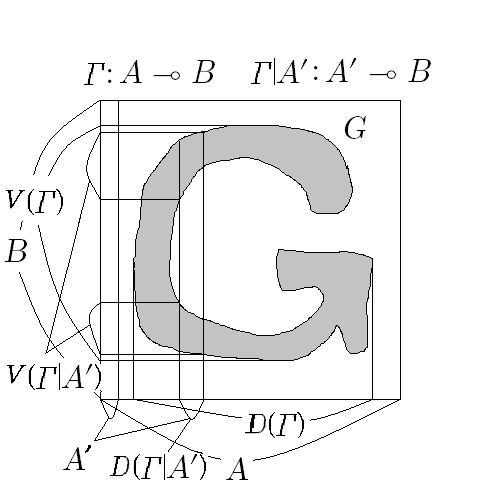
\includegraphics[width=160pt]{1.2.1.a.png}
\end{center}
2つの対応たち$\varGamma:A \multimap B$、$\varDelta:A \multimap B$が与えられたとき、これらの対応たちが等しいかどうかの判定法として、定理\ref{1.2.1.17}が知られており、$\forall a \in A$に対し、$\varGamma\left( \left\{ a \right\} \right) = \varDelta\left( \left\{ a \right\} \right)$が成り立つならそのときに限り、$\varGamma:A \multimap B = \varDelta:A \multimap B$が成り立つことを主張しているのであった。さらに、対応について次のことも成り立つことが知られている。
\begin{thm*}[定理\ref{1.2.2.6}の再掲]
次のことが成り立つ。
\begin{itemize}
\item
  2つの集合たち$A$、$B$の直積$A \times B$とこれの部分集合$G$が与えられれば、対応$\varGamma:A \multimap B = (A \times B,G)$が一意的に決まる。
\item
  1つの対応$\varGamma:A \multimap B$について$A'\in \mathfrak{P}(A)$なる集合$A'$を用いて$V\left( \varGamma|A' \right) = \bigcup_{a \in A'} {V\left( \varGamma|\left\{ a \right\} \right)}$が成り立つ。
\end{itemize}
\end{thm*}
対応$\varGamma:A \multimap B = (A \times B,G)$において、$\forall(a,b) \in A \times B$に対し、$(a,b) \in G \Leftrightarrow (b,a) \in H$となるような対応$(B \times A,H)$も考えられることができ、これをその対応$\varGamma:A \multimap B$の逆対応といい$\varGamma^{- 1}:B \multimap A$と書くのであった。ここで、その対応$\varGamma^{- 1}$によるその集合$B$の部分集合$B'$の像$V\left( \varGamma^{- 1}|B' \right)$をその対応$\varGamma$によるその集合$B'$の原像、逆像などという。\par
対応$\varGamma:A \multimap B = (A \times B,G)$の逆対応$\varGamma^{- 1}$が$\varGamma^{- 1}:B \multimap A = (B \times A,H)$と与えられたとき、これのgraph$H$については定理\ref{1.2.1.18}より$H = \left\{ (b,a) \in B \times A \middle| (a,b) \in G \right\}$が成り立つのであった。さらに、次のことも成り立つことが知られている。
\begin{thm*}[定理\ref{1.2.2.7}の再掲]
対応$\varGamma:A \multimap B = (A \times B,G)$において、次式たちが成り立つ。
\begin{align*}
\left( \varGamma^{- 1} \right)^{- 1} &= \varGamma\\
D\left( \varGamma^{- 1} \right) &= V(\varGamma)\\
V\left( \varGamma^{- 1} \right) &= D(\varGamma)
\end{align*}
\end{thm*}
\begin{thm}\label{1.2.3.1}
対応$\varGamma:A \multimap B$において、$\forall A'\in \mathfrak{P}(A)$に対し、$A'=\emptyset $が成り立つなら、$V(\varGamma |A')=\emptyset $が成り立つ。
\end{thm}
\begin{proof}
対応$\varGamma:A \multimap B$において、$\forall A'\in \mathfrak{P}(A)$に対し、$A' = \emptyset$が成り立つなら、$a \in A'$が成り立つような元$a$が存在しないので、その対応$\varGamma$のgraphを$G$とおくと、論理式$\exists a \in A'\left[ (a,b) \in G \right]$もやはり偽となる。したがって、$\forall b \in B$に対し、次のようになる。
\begin{align*}
b \in V\left( \varGamma|A' \right) &\Leftrightarrow b \in B \land \exists a \in A'\left[ (a,b) \in G \right]\\
&\Leftrightarrow b \in B \land \bot\\
&\Leftrightarrow b \in \left\{ b \in B \middle| \bot \right\}\\
&\Leftrightarrow b \in \emptyset
\end{align*}
よって、$V\left( \varGamma|A' \right) = \emptyset$が成り立つ。
\end{proof}
\begin{thm}
\label{1.2.3.2}
対応$\varGamma:A \multimap B$において、$\forall a \in A\forall b \in B$に対し、$b \in V\left( \varGamma|\left\{ a \right\} \right)$が成り立つならそのときに限り、$a \in V\left( \varGamma^{- 1}|\left\{ b \right\} \right)$が成り立つ。
\end{thm}
\begin{proof}
対応$\varGamma:A \multimap B$において、$\forall a \in A\forall b \in B$に対し、その対応$\varGamma$のgraphを$G$、その逆対応$\varGamma^{-1}$のgraphを$H$とおくと、次のようになる。
\begin{align*}
b \in V\left( \varGamma|\left\{ a \right\} \right) &\Leftrightarrow b \in \left\{ b \in B \middle| \exists a \in \left\{ a \right\}\left[ (a,b) \in G \right] \right\}\\
&\Leftrightarrow a \in A \land b \in B \land (a,b) \in G\\
&\Leftrightarrow a \in \left\{ a \in A \middle| \exists b \in \left\{ b \right\}\left[ (a,b) \in G \right] \right\}\\
&\Leftrightarrow a \in \left\{ a \in A \middle| \exists b \in \left\{ b \right\}\left[ (b,a) \in H \right] \right\}\\
&\Leftrightarrow a \in V\left( \varGamma^{- 1}|\left\{ b \right\} \right)
\end{align*}
\end{proof}
%\hypertarget{ux5199ux50cf-1}{%
\subsubsection{写像}%\label{ux5199ux50cf-1}}
対応$f:A \multimap B$について、$\forall a \in A\exists b \in B$に対し、$V\left( f|\left\{ a \right\} \right) = \left\{ b \right\}$が成り立つとき、その対応$f$を写像といい$f:A \rightarrow B$、$A\overset{f}{\rightarrow}B$などと書く。この写像$f:A \rightarrow B$全体の集合を$\mathfrak{F}(A,B)$、$B^{A}$などと書く。このとき、$V\left( f|\left\{ a \right\} \right) = \left\{ b \right\}$のことを、単に、$f(a) = b$と書き、これを明示するとき、その写像$f$を$f:A \rightarrow B;a \mapsto f(a) = b$などと書くときがありその元$b$をその元$a$のその写像$f$による像、その元$a$におけるその写像$f$の値などといいこのことをその写像$f$はその元$a$をその元$b$に写す、その元$a$にその元$b$を対応させるなどという。\par
これらの用語たちは次の図のように該当される。
\begin{center}
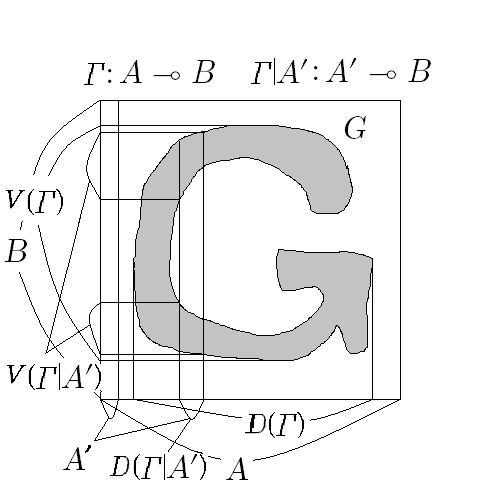
\includegraphics[width=160pt]{1.2.1.a.png}
\end{center}
\begin{thm}
\label{1.2.3.3}
対応$\varGamma:A \multimap B$と写像$f:A \rightarrow B$について、$A',A''\in \mathfrak{P}(A)$、$B',B''\in \mathfrak{P}(B)$なる集合たち$A'$、$A''$、$B'$、$B''$を用いると、次式が成り立つ。
\begin{align*}
A' \subseteq A'' &\Rightarrow V\left( \varGamma|A' \right) \subseteq V\left( \varGamma|A'' \right)\\
V\left( \varGamma|\bigcup_{A \in \mathcal{A}} A \right) &= \bigcup_{A \in \mathcal{A}} {V\left( \varGamma|A \right)}\\
V\left( \varGamma|\bigcap_{A \in \mathcal{A}} A \right) &\subseteq \bigcap_{A \in \mathcal{A}} {V\left( \varGamma|A \right)}\\
V\left( f^{- 1}|\bigcap_{B\in \mathcal{B}} B \right) &= \bigcap_{B\in \mathcal{B}} {V\left( f^{- 1}|B \right)}\\
V\left( \varGamma|A \setminus A' \right) &\supseteq V\left( \varGamma|A \right) \setminus V\left( \varGamma|A' \right)\\
V\left( f^{- 1}|B \setminus B' \right) &= A \setminus V\left( f^{- 1}|B' \right)\\
V\left( f^{- 1}|V\left( f|A' \right) \right) &\supseteq A'\\
V\left( f|V\left( f^{- 1}|B' \right) \right) &\subseteq B'
\end{align*}
\end{thm}
\begin{proof}
定理\ref{1.2.2.8}と定理\ref{1.2.2.9}そのものである。
\end{proof}
\begin{dfn}
後述する$n$次元数空間$\mathbb{R}^{n}$の部分集合たち$A$、$B$を用いた写像$f:A \rightarrow B$は特に関数といわれる。
\end{dfn}
\begin{dfn}
$b \in B$なる元$b$が1つ決められたとき、次式のような写像$f$は特に定値写像などといわれる。
\begin{align*}
f:A \rightarrow B;a \mapsto b
\end{align*}
\end{dfn}
\begin{dfn}
次式のような写像$f$はその集合$A$における恒等写像などといわれ$I_{A}$、$1_{A}$、$\mathrm{id}_{A}$などと書かれることが多い。
\begin{align*}
f:A \rightarrow A;a \mapsto a
\end{align*}
\end{dfn}
\begin{thm}
\label{1.2.3.4}
任意の写像$f:A \rightarrow B$において、$A = D(f)$が成り立つ。
\end{thm}\par
これにより、明らかに$\forall A'\in \mathfrak{P}(A)$に対し、$A' = D\left( f|A' \right)$が成り立つ。しかしながら、終集合と値域は必ずしも一致するとは限らないことに注意されたい。
\begin{proof}
任意の写像$f:A \rightarrow B$において、$D(f) \subset A$が成り立つとき、$a \in A \setminus D(f)$なる元$a$を考えると、次式が成り立ち、
\begin{align*}
a \notin D(f) = \left\{ a \in A \middle| V(f) \neq \emptyset \right\}
\end{align*}
$a \in A$が成り立つことに注意すれば、$V(f) = \emptyset$が成り立つことになり、写像$f|\left\{ a \right\}$が与えられれば、やはり$V\left( f|\left\{ a \right\} \right) = \emptyset$が成り立つことになるが、これは写像の定義に反する。したがって、$D(f) \subseteq A$が成り立って$D(f) \subset A$は成り立たない。ここで、$D(f) \subseteq A$が成り立つならそのときに限り、$D(f) = A$または$D(f) \subset A$が成り立つことに注意すれば、よって、$A = D(f)$が成り立つ。
\end{proof}
\begin{thm}
\label{1.2.3.5}
写像$f:A \rightarrow B$において、次式が成り立つ。
\begin{align*}
V(f) = \left\{ f(a) \in B \middle| \exists a \in A\left[ f(a) \in B \right] \right\}
\end{align*}
\end{thm}
\begin{proof}
写像$f:A \rightarrow B$において、定義より$\forall a \in A$に対し、次式が成り立つのであった。
\begin{align*}
V\left( f|\left\{ a \right\} \right) = \left\{ b \right\} \Leftrightarrow f(a) = b \in B
\end{align*}
ここで、$\forall b \in V(f)$に対し、その写像$f$のgraphを$G$とおきその集合$A$のある元の1つを$\overline{a}$とおくと、次のようになる。
\begin{align*}
b \in V(f) &\Leftrightarrow b \in \left\{ b \in B \middle| \exists a \in A\left[ (a,b) \in G \right] \right\}\\
&\Leftrightarrow b \in B \land \exists a \in A\left[ (a,b) \in G \right]\\
&\Leftrightarrow b \in B \land \overline{a} \in A \land \left( \overline{a},b \right) \in G\\
&\Leftrightarrow b \in B \land \overline{a} \in \bigcup_{a \in A} \left\{ a \right\} \land \left( \overline{a},b \right) \in G\\
&\Leftrightarrow b \in B \land \exists a \in A\left[ \overline{a} \in \left\{ a \right\} \right] \land \left( \overline{a},b \right) \in G\\
&\Leftrightarrow b \in B \land \overline{a} \in A \land \overline{a} \in \left\{ \overline{a} \right\} \land \left( \overline{a},b \right) \in G\\
&\Leftrightarrow b \in B \land \overline{a} \in A \land \exists a \in \left\{ a \right\}\left[ (a,b) \in G \right]\\
&\Leftrightarrow \overline{a} \in A \land b \in \left\{ b \in B \middle| \exists a \in \left\{ a \right\}\left[ (a,b) \in G \right] \right\}\\
&\Leftrightarrow \overline{a} \in A \land b \in V\left( f|\left\{ a \right\} \right)\\
&\Leftrightarrow \overline{a} \in A \land V\left( f|\left\{ a \right\} \right) = \left\{ b \right\}\\
&\Leftrightarrow \overline{a} \in A \land f(a) = b \in B\\
&\Leftrightarrow f(a) = b \in B \land \exists a \in A\left[ f(a) \in B \right]\\
&\Leftrightarrow b \in \left\{ f(a) \in B \middle| \exists a \in A\left[ f(a) \in B \right] \right\}
\end{align*}
よって、$V(f) = \left\{ f(a) \in B \middle| \exists a \in A\left[ f(a) \in B \right] \right\}$が成り立つ。
\end{proof}
\begin{thm}
\label{1.2.3.6}
写像$f:A \rightarrow B$において、$\forall A'\in \mathfrak{P}(A)$に対し、$A' = \emptyset$が成り立つならそのときに限り、$V\left( f|A' \right) = \emptyset$が成り立つ。
\end{thm}
\begin{proof}
任意の写像$f:A \rightarrow B$について、$\forall A'\in \mathfrak{P}(A)$に対し、$A' = \emptyset$が成り立つなら、$V\left( f|A' \right) = \emptyset$が成り立つことは上記の議論によりすでに示されている。$V\left( f|A' \right) = \emptyset$が成り立つとき、上記の定理より次式が成り立つ。
\begin{align*}
V\left( f \middle| A' \right) = \left\{ f(a) \in B \middle| \exists a \in A'\left[ f(a) \in B \right] \right\}
\end{align*}
ここで、$A' \neq \emptyset$が成り立つと仮定すると、$\forall b \in V\left( f \middle| A' \right)$に対し、次式が成り立つ。
\begin{align*}
b = f(a) \in B \land \exists a \in A'\left[ f(a) \in B \right] \Leftrightarrow b = f(a) \in B \land \bot
\end{align*}
これにより、次式が成り立つ。
\begin{align*}
\left( \forall a \in A'\left[ f(a) \notin B \right] \land \top \right) \vee \left( \exists a \in A'\left[ f(a) \in B \right] \land \bot \right)
\end{align*}
したがって、$\forall a \in A'$に対し、$f(a) \notin B$が成り立つ。ここで、その対応$f$は写像なので、$A' = D\left( f|A' \right)$が成り立つ。定義域の定義より次式が成り立つ。
\begin{align*}
D\left( f|A' \right) = \left\{ a \in A \middle| V\left( f|A' \right) \neq \emptyset \right\}
\end{align*}
ここで、値域の定義より$\forall a \in A'$に対し、次式が成り立つ。
\begin{align*}
a \in A \land b \in B \land \exists a \in A'\left[ f(a) \in B \right]
\end{align*}
このことは、$\forall a \in A'$に対し、$f(a) \notin B$が成り立つことに矛盾する。したがって、$A' = \emptyset$が成り立つ。
\end{proof}
%\hypertarget{ux5168ux5358ux5c04}{%
\subsubsection{全単射}%\label{ux5168ux5358ux5c04}}
\begin{dfn}
写像$f:A \rightarrow B$が$V(f) = B$を満たすとき、その写像$f$は全射であるといい$f:A \twoheadrightarrow B$などと書く。
\end{dfn}
\begin{thm}
\label{1.2.3.7}
写像$f:A \rightarrow B$について、次のことは同値である。
\begin{itemize}
\item
  写像$f:A \rightarrow B$は全射である。
\item
  $\forall b \in B\exists a \in A$に対し、$f(a) = b$が成り立つ。
\item
  その対応$f^{- 1}$をその集合$B$の任意の元$b$からなる集合$\left\{ b \right\}$に制限したときの対応$f^{- 1}|\left\{ b \right\}$の値域$V\left( f^{- 1}|\left\{ b \right\} \right)$は空集合でない、即ち、$\forall b \in B$に対し、$V\left( f^{- 1}|\left\{ b \right\} \right) \neq \emptyset$が成り立つ。
\end{itemize}
\end{thm}
\begin{proof}
全射な写像$f:A \twoheadrightarrow B$が与えられたとする。$\forall b \in B$に対し、全射の定義より$V(f) = B$が成り立つので、$b \in V(f)$が成り立つ。ここで、上記の定理より次式が成り立つ。
\begin{align*}
V(f) = \left\{ f(a) \in B \middle| \exists a \in A\left[ f(a) \in B \right] \right\}
\end{align*}
したがって、次式が成り立つ。
\begin{align*}
f(a) = b \in B \land \exists a \in A\left[ f(a) = b \in B \right]
\end{align*}
ゆえに、$\forall b \in B\exists a \in A$に対し、$f(a) = b$が成り立つ。\par
これが成り立つなら、$\forall b \in B$に対し、次式が成り立つ。
\begin{align*}
\exists a \in A\left[ a \in V\left( f^{- 1}|\left\{ b \right\} \right) \right]
\end{align*}
したがって、その集合$V\left( f^{- 1} \middle| \left\{ b \right\} \right)$は空集合ではないことになりその対応$f^{- 1}$をその集合$B$の任意の元$b$からなる集合$\left\{ b \right\}$に制限したときの対応$f^{- 1}|\left\{ b \right\}$の値域$V\left( f^{- 1}|\left\{ b \right\} \right)$は空集合でない、即ち、$V\left( f^{- 1}|\left\{ b \right\} \right) \neq \emptyset$が成り立つことが示された。\par
また、これが成り立つなら、$\forall b \in B\exists a \in A$に対し、$a \in V\left( f^{- 1}|\left\{ b \right\} \right)$が成り立つ。ここで、値域の定義より次のようになる。
\begin{align*}
a \in V\left( f^{- 1}|\left\{ b \right\} \right) &\Leftrightarrow a \in A \land \exists b \in \left\{ b \right\}\left[ (a,b) \in G \right]\\
&\Leftrightarrow a \in A \land (a,b) \in G\\
&\Rightarrow \exists a \in A\left[ (a,b) \in G \right]
\end{align*}
ここで、$b \in B$が成り立つことに注意すれば、次のようになり、
\begin{align*}
b \in B \land \exists a \in A\left[ (a,b) \in G \right] &\Leftrightarrow b \in \left\{ b \in B \middle| \exists a \in A\left[ (a,b) \in G \right] \right\}\\
&\Leftrightarrow b \in V(f)
\end{align*}
したがって、$B \subseteq V(f)$が成り立つ。逆に、その集合$V(f)$は定義より明らかにその集合$B$の部分集合であったので、$V(f) \subseteq B$が成り立つ。したがって、$V(f) = B$が成り立つ。これにより、その写像$f$は全射である。
\end{proof}
\begin{dfn}
写像$f:A \rightarrow B$が、$\forall a,b \in A$に対し、$a \neq b$が成り立つなら、$f(a) \neq f(b)$が成り立つとき、その写像$f$は単射であるといい$f:A \rightarrowtail B$などと書く。
\end{dfn}
\begin{thm}
\label{1.2.3.8}
写像$f:A \rightarrow B$において、次のことは同値である。
\begin{itemize}
\item
  写像$f:A \rightarrow B$は単射である。
\item
  $\forall f(a),f(b) \in V(f)$に対し、$f(a) = f(b)$が成り立つなら、$a = b$が成り立つ。
\item
  $\forall b \in V(f)\exists a \in A$に対し、$V\left( f^{- 1}|\left\{ b \right\} \right) = \left\{ a \right\}$が成り立つ。
\end{itemize}
\end{thm}
\begin{proof}
単射な写像$f:A \rightarrowtail B$が与えられたとする。$\forall f(a),f(b) \in V(f)$に対し、$a,b \in A$なる元々$a$、$b$が存在しているので、したがって、$a \neq b$が成り立つなら、$f(a) \neq f(b)$が成り立つ。対偶律より$f(a) = f(b)$が成り立つなら、$a = b$が成り立つ。\par
逆に、$\forall f(a),f(b) \in V(f)$に対し、$f(a) = f(b)$が成り立つなら、$a = b$が成り立つとする。$\forall a,b \in A$に対し、$f(a) = f(b)$が成り立つなら、$a = b$が成り立つので、対偶律により$a \neq b$が成り立つなら、$f(a) \neq f(b)$が成り立つので、その写像$f:A \rightarrow B$は単射である。\par
また、$\forall f(a),f(b) \in V(f)$に対し、$f(a) = f(b)$が成り立つなら、$a = b$が成り立つとき、その対応$f^{- 1}$をその集合$B$の任意の元$b$からなる集合$\left\{ b \right\}$に制限したときの対応$f^{- 1}|\left\{ b \right\}$の値域$V\left( f^{- 1}|\left\{ b \right\} \right)$について、その写像のgraphを$G$とおくと、値域の定義より次式が成り立つ。
\begin{align*}
V\left( f^{- 1}|\left\{ b \right\} \right) = \left\{ a \in A \middle| \exists b \in \left\{ b \right\}\left[ (a,b) \in G \right] \right\} = \left\{ a \in A \middle| (a,b) \in G \right\}
\end{align*}
ここで、その集合$\left\{ b \right\}$は明らかに空集合ではないので、その集合$V\left( f^{- 1}|\left\{ b \right\} \right)$も空集合ではないことになり$a \in V\left( f^{- 1}|\left\{ b \right\} \right)$なる元$a$がとれる。ここで、$a_{1},a_{2} \in V\left( f^{- 1}|\left\{ b \right\} \right)$かつ$a_{1} \neq a_{2}$なる元々$a_{1}$、$a_{2}$がとられると、$b \in V\left( f|\left\{ a_{1} \right\} \right)$かつ$b \in V\left( f|\left\{ a_{2} \right\} \right)$が成り立つ。ここで、その対応$f$は写像なので、次式が成り立つ。$V\left( f|\left\{ a_{1} \right\} \right) = \left\{ b \right\}$かつ$V\left( f|\left\{ a_{2} \right\} \right) = \left\{ b \right\}$が成り立つ。したがって、$f\left( a_{1} \right) = f\left( a_{2} \right) = b$が成り立つ。ここで、仮定より$a_{1} = a_{2}$が成り立つことになるが、これは仮定の$a_{1} \neq a_{2}$に矛盾する。したがって、$a \in V\left( f^{- 1}|\left\{ b \right\} \right)$が成り立つような元$a$はただ1つのみとなり$V\left( f^{- 1}|\left\{ b \right\} \right) = \left\{ a \right\}$が成り立つ。\par
逆に、これが成り立つとき、$\forall f(a),f(b) \in V(f)$に対し、$f(a) = f(b)$が成り立つなら、$V\left( f^{- 1}|\left\{ f(a) \right\} \right) = \left\{ a \right\}$かつ$V\left( f^{- 1}|\left\{ f(b) \right\} \right) = \left\{ b \right\}$が成り立つので、$\left\{ a \right\} = \left\{ b \right\}$が得られ、したがって、$a = b$が成り立つ。
\end{proof}
\begin{thm}
\label{1.2.3.9}
写像$f:A \rightarrow B$について、次のことが成り立つ。
\begin{itemize}
\item
  その写像$f$が単射であるとき、$\mathcal{A \in}\mathfrak{P}\left( \mathfrak{P}(A) \right)$なる集合$\mathcal{A}$と$\mathcal{B \in}\mathfrak{P}\left( \mathfrak{P}(B) \right)$なる集合$\mathcal{B}$に対し、次式が成り立つ。
\begin{align*}
V\left( f|\bigcap_{A \in \mathcal{A}} A \right) = \bigcap_{A \in \mathcal{A}} {V\left( f|A \right)}
\end{align*}
\item
  その写像$f$が単射であるとき、$A'\in \mathfrak{P}(A)$なる集合$A'$を用いて次式が成り立つ。
\begin{align*}
V\left( f|A \setminus A' \right) = V\left( f|A \right) \setminus V\left( f|A' \right)
\end{align*}
\item
  その写像$f$が単射であるとき、$A'\in \mathfrak{P}(A)$なる集合$A'$を用いて次式が成り立つ。
\begin{align*}
V\left( f^{- 1} \middle| V\left( f|A' \right) \right) = A'
\end{align*}
\item
  その写像$f$が全射であるとき、$B'\in \mathfrak{P}(B)$なる集合$B'$を用いて次式が成り立つ。
\begin{align*}
V\left( f \middle| V\left( f^{- 1}|B' \right) \right) = B'
\end{align*}
\end{itemize}
\end{thm}
\begin{proof}
写像$f:A \rightarrow B$について、$\mathcal{A \in}\mathfrak{P}\left( \mathfrak{P}(A) \right)$なる集合$\mathcal{A}$と$\mathcal{B \in}\mathfrak{P}\left( \mathfrak{P}(B) \right)$なる集合$\mathcal{B}$に対し、次式が成り立つ。
\begin{align*}
V\left( f|\bigcap_{A \in \mathcal{A}} A \right) \subseteq \bigcap_{A \in \mathcal{A}} {V\left( f|A \right)}
\end{align*}
その写像$f$が単射であるとき、$\forall b \in \bigcap_{A \in \mathcal{A}} {V\left( f|A \right)}$に対し、次式が成り立つ。
\begin{align*}
b \in \bigcap_{A \in \mathcal{A}} {V\left( f|A \right)} \Leftrightarrow \forall A \in \mathcal{A}\left[ b \in V\left( f|A \right) \right]
\end{align*}
ここで、値域の定義より次のようになる。
\begin{align*}
b \in \bigcap_{A \in \mathcal{A}} {V\left( f|A \right)} &\Leftrightarrow \forall A \in \mathcal{A}\left[ b \in B \land \exists a_{A} \in A\left[ f\left( a_{A} \right) = b \right] \right]\\
&\Leftrightarrow \forall A \in \mathcal{A\exists}a_{A} \in A\left[ b \in B \land f\left( a_{A} \right) = b \right]
\end{align*}
ここで、その写像$f$は単射であるので、$\forall A,B \in \mathcal{A}$に対し、$f\left( a_{A} \right) = f\left( a_{B} \right) = b$が成り立つなら、$a_{A} = a_{B}$が成り立つので、その元$a_{A}$はその集合$A$によらなく$a$とおかれると、全称除去、存在除去、全称導入、存在導入より次のようになる。
\begin{align*}
b \in \bigcap_{A \in \mathcal{A}} {V\left( f|A \right)} &\Rightarrow \forall A \in \mathcal{A\exists}a \in A\left[ b \in B \land f(a) = b \right]\\
&\Leftrightarrow \forall A \in \mathcal{A}[ a \in A] \land b \in B \land f(a) = b\\
&\Leftrightarrow a \in \bigcap_{A \in \mathcal{A}} A \land b \in B \land f(a) = b\\
&\Leftrightarrow \exists a \in \bigcap_{A \in \mathcal{A}} A\left[ b \in B \land f(a) = b \right]\\
&\Leftrightarrow b \in B \land \exists a \in \bigcap_{A \in \mathcal{A}} A\left[ f(a) = b \right]
\end{align*}
値域の定義より次式が成り立つので、
\begin{align*}
b \in \bigcap_{A \in \mathcal{A}} {V\left( f|A \right)} \Rightarrow b \in V\left( f|\bigcap_{A \in \mathcal{A}} A \right)
\end{align*}
$V\left( f|\bigcap_{A \in \mathcal{A}} A \right) \supseteq \bigcap_{A \in \mathcal{A}} {V\left( f|A \right)}$が得られ、よって、$V\left( f|\bigcap_{A \in \mathcal{A}} A \right) = \bigcap_{A \in \mathcal{A}} {V\left( f|A \right)}$が成り立つ。\par
写像$f:A \rightarrow B$について、$A'\in \mathfrak{P}(A)$なる集合$A'$を用いて次式が成り立つ。
\begin{align*}
V\left( f|A \setminus A' \right) \supseteq V\left( f|A \right) \setminus V\left( f|A' \right)
\end{align*}
その写像$f$が単射であるとき、$\forall b \in V\left( f|A \setminus A' \right)$に対し、値域の定義より次のようになり
\begin{align*}
b \in V\left( f|A \setminus A' \right) &\Leftrightarrow b \in B \land \exists a \in A \setminus A'\left[ f(a) = b \right]\\
&\Leftrightarrow b \in B \land \exists a \in A\left[ a \notin A' \land f(a) = b \right]
\end{align*}
$\forall a' \in A'$に対し、$f(a) = b$となるその集合$A \setminus A'$の元$a$を用いて$a \neq a'$が成り立つかつ、その写像$f$は単射であるので、$f(a) = b \neq f\left( a' \right)$が成り立つ。したがって、次のようになる。
\begin{align*}
b \in V\left( f|A \setminus A' \right) \Rightarrow b \in B \land \exists a \in A\left[ f(a) = b \right] \land \forall a' \in A'\left[ f\left( a' \right) \neq b \right]\\
&\Leftrightarrow b \in V\left( f|A \right) \setminus V\left( f|A' \right)
\end{align*}
したがって、$V\left( f|A \setminus A' \right) \subseteq V\left( f|A \right) \setminus V\left( f|A' \right)$が得られ、よって、$V\left( f|A \setminus A' \right) = V\left( f|A \right) \setminus V\left( f|A' \right)$が成り立つ。\par
写像$f:A \rightarrow B$について、$A'\in \mathfrak{P}(A)$なる集合$A'$を用いて次式が成り立つ。
\begin{align*}
V\left( f^{- 1} \middle| V\left( f|A' \right) \right) \supseteq A'
\end{align*}
その写像$f$が単射であるとき、$\forall a \in V\left( f^{- 1} \middle| V\left( f|A' \right) \right)$に対し、値域の定義と存在除去より次のようになる。
\begin{align*}
a \in V\left( f^{- 1} \middle| V\left( f|A' \right) \right) &\Leftrightarrow a \in A \land \exists b \in V\left( f|A' \right)\left[ f(a) = b \right]\\
&\Leftrightarrow a \in A \land b \in V\left( f|A' \right) \land f(a) = b\\
&\Leftrightarrow a \in A \land b \in B \land \exists a' \in A'\left[ f\left( a' \right) = b \right] \land f(a) = b\\
&\Rightarrow a \in A \land \exists a' \in A'\left[ f(a) = f\left( a' \right) \right]
\end{align*}
その写像$f$は単射であるので、$f(a) = f\left( a' \right)$が成り立つなら、$a = a'$が成り立つことになり、したがって、$a \in A'$が成り立つ。これにより、$V\left( f^{- 1} \middle| V\left( f|A' \right) \right) \subseteq A'$が得られ、よって、$V\left( f^{- 1} \middle| V\left( f|A' \right) \right) = A'$が成り立つ。\par
写像$f:A \rightarrow B$について、$B'\in \mathfrak{P}(B)$なる集合$B'$を用いて次式が成り立つ。
\begin{align*}
V\left( f \middle| V\left( f^{- 1}|B' \right) \right) \subseteq B'
\end{align*}
その写像$f$が全射であるとき、$\forall b \in B'$に対し、$V\left( f^{- 1}|\left\{ b \right\} \right) \subseteq V\left( f^{- 1}|B' \right)$が成り立つ。ここで、その写像$f$が全射なので、その集合$V\left( f^{- 1}|\left\{ b \right\} \right)$は空集合ではなく$a \in V\left( f^{- 1}|\left\{ b \right\} \right)$なる元$a$がその集合$A$に存在する。したがって、次のようになる。
\begin{align*}
f(a) \in V\left( f|V\left( f^{- 1}|\left\{ b \right\} \right) \right) \subseteq V\left( f \middle| V\left( f^{- 1}|B' \right) \right)
\end{align*}
ここで、その値域$V\left( f^{- 1}|\left\{ b \right\} \right)$の定義より$f(a) = b$が成り立つので、$b \in V\left( f \middle| V\left( f^{- 1}|B' \right) \right)$が成り立つ。これにより、$V\left( f \middle| V\left( f^{- 1}|B' \right) \right) \supseteq B'$が得られ、よって、$V\left( f \middle| V\left( f^{- 1}|B' \right) \right) = B'$が成り立つ。
\end{proof}
\begin{dfn}
写像$f:A \rightarrow B$が全射であるかつ、単射であるとき、その写像$f$は全単射である、双射であるなどといい$f:A\overset{\sim}{\rightarrow}B$、$f:\text{\raisebox{-1mm}{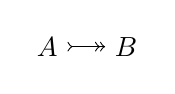
\begin{tikzpicture}[auto]
  \node (a) at (0, 0) {$A$};
  \node (b) at (1, 0) {$B$};
  \draw [>->>] (a) to node {} (b);
  \end{tikzpicture} } } $などと書く\footnote{圏論でいえばその記号は双射である、即ち、逆写像をもつような写像であることを意味してて写像であれば全単射ならそのときにかぎり逆写像をもつといえますが、圏論で扱う射では必ずしもそうとはいえなく全単射だからその記号がいつでも使えるというわけではないことに注意するといいかと思います。}。
\end{dfn}
\begin{thm}
\label{1.2.3.10}
写像$f:A \rightarrow B$について、次のことは同値である。
\begin{itemize}
\item
  その写像$f$は全単射である。
\item
  $\forall b \in B\exists!a \in A$に対し、$f(a) = b$が成り立つ。
\item
  写像$f:A \rightarrow B$の値域$V(f)$について、$V(f) = B$が成り立つかつ、$\forall f(a),f(b) \in B$に対し、$f(a) = f(b)$が成り立つなら、$a = b$が成り立つ。
\item
  $\forall b \in B\exists a \in A$に対し、$V\left( f^{- 1}|\left\{ b \right\} \right) = \left\{ a \right\}$が成り立つ。
\end{itemize}
\end{thm}
\begin{proof}
全単射な写像$f:A\overset{\sim}{\rightarrow}B$が与えられたとする。このとき、その写像$f$は全射でもあるので、$\forall b \in B\exists a \in A$に対し、$f(a) = b$が成り立つ。ここで、このような2つの元々$a$、$a'$がとられ$a \neq a'$が成り立つと仮定すると、その写像$f$は単射でもあるので、$f(a) = f\left( a' \right)$が成り立つ。これは仮定の$f(a) = f\left( a' \right) = b$に矛盾する。したがって、$\forall b \in B\exists!a \in A$に対し、$f(a) = b$が成り立つ。\par
逆に、これが成り立つなら、$\forall b \in B\exists a \in A$に対し、$f(a) = b$が成り立つので、その写像$f$は全射である。したがって、$B = V(f)$が成り立つ。さらに、$\forall b \in V(f) = B$に対し、明らかに$b \in V\left( f|\left\{ a \right\} \right)$が成り立つので、$a \in V\left( f^{- 1}|\left\{ b \right\} \right)$も成り立つ。ここで、仮定よりこのような元$a$はただ1つ存在するのであったので、$V\left( f^{- 1}|\left\{ b \right\} \right) = \left\{ a \right\}$が成り立つ。その写像$f$は単射でもあり、したがって、その写像$f$は全単射である。\par
その写像$f$が全単射であるなら、その写像$f$は単射でもあるので、$\forall f(a),f(b) \in B$に対し、$f(a) = f(b)$が成り立つなら、$a = b$が成り立つ。さらに、その写像$f$は全射であるので、$V(f) = B$が成り立つ。したがって、$V(f) = B$が成り立つかつ、$\forall f(a),f(b) \in B$に対し、$f(a) = f(b)$が成り立つなら、$a = b$が成り立つ。\par
逆に、これが成り立つなら、$V(f) = B$が成り立つので、その写像$f$は全射である。ここで、$\forall f(a),f(b) \in B$に対し、$f(a) = f(b)$が成り立つなら、$a = b$が成り立つので、その写像$f$は単射である。したがって、その写像$f$は全単射である。\par
また、その写像$f$が全単射であるなら、その写像$f$は単射でもあるので、$\forall b \in V(f)\exists a \in A$に対し、$V\left( f^{- 1}|\left\{ b \right\} \right) = \left\{ a \right\}$が成り立つ。さらに、その写像$f$は全射でもあり$V(f) = B$が成り立つので、$\forall b \in B\exists a \in A$に対し、$V\left( f^{- 1}|\left\{ b \right\} \right) = \left\{ a \right\}$が成り立つ。\par
逆に、これが成り立つなら、$V(f) \subseteq B$が成り立つので、その写像$f$は単射である。さらに、次のようになるので、
\begin{align*}
V\left( f|\left\{ a \right\} \right) = V\left( f|V\left( f^{- 1}|\left\{ b \right\} \right) \right) \subseteq \left\{ b \right\}
\end{align*}
$\forall b \in B\exists a \in A$に対し、$f(a) = b$が成り立ち、したがって、その写像$f$は全射である。以上より、その写像$f$は全単射である。
\end{proof}
%\hypertarget{ux6a19ux6e96ux7684ux5358ux5c04}{%
\subsubsection{標準的単射}%\label{ux6a19ux6e96ux7684ux5358ux5c04}}
\begin{thm}
\label{1.2.3.11}
集合$A$が与えられたとき、$\forall A'\in \mathfrak{P}(A)$に対し、次式のような写像$i$が考えられる。
\begin{align*}
i:A' \rightarrow A;a \mapsto a
\end{align*}
これについて、次のことが成り立つ。
\begin{itemize}
\item
  その写像$i$は単射である。
\item
  その写像$i$の値域$V(i)$について、$V(i) = A'$が成り立つ。
\item
  $A' = A$が成り立つなら、その写像$i$は全単射となる。
\end{itemize}
\end{thm}
\begin{dfn}
このような写像$i$を特にその集合$A'$からその集合$A$への標準的単射、自然な単射、包含写像などといい$A' \hookrightarrow A$などと書く。
\end{dfn}
\begin{proof}
集合$A$が与えられたとき、$\forall A'\in \mathfrak{P}(A)$に対し、次式のような写像$i$が考えられる。
\begin{align*}
i:A' \rightarrow A;a \mapsto a
\end{align*}
ここで、$\forall a,b \in A'$に対し、$a \neq b$が成り立つなら、$i(a) = a$かつ$i(b) = b$が成り立つので、$i(a) \neq i(b)$が成り立つ。これにより、その写像$i$は単射となる。\par
また、その写像$i$の値域$V(i)$について、$V(i) = \bigcup_{a \in A'} {V\left( i|\left\{ a \right\} \right)}$が成り立つのであった。したがって、その対応$i$が写像であるので、$V\left( i|\left\{ a \right\} \right) = \left\{ i(a) \right\}$が成り立つことに注意すれば、次式のようになる。
\begin{align*}
V(i) = \bigcup_{a \in A'} {V\left( i|\left\{ a \right\} \right)} = \bigcup_{a \in A'} \left\{ i(a) \right\} = \bigcup_{a \in A'} \left\{ a \right\} = A'
\end{align*}\par
$A' = A$が成り立つなら、上記の議論により$V(i) = A' = A$が成り立つので、定義より明らかにその写像$i$は全射である。したがって、その写像$i$は全単射となる。
\end{proof}
%\hypertarget{ux9006ux5199ux50cf}{%
\subsubsection{逆写像}%\label{ux9006ux5199ux50cf}}
\begin{dfn}
写像$f$の逆対応$f^{- 1}$は必ずしも写像になるとは限らないが、写像になるときがありこの写像$f^{- 1}$をその写像$f$の逆写像という。
\end{dfn}
\begin{thm}
\label{1.2.3.12}
写像$f$が全単射であるならそのときに限り、その写像$f$の逆写像$f^{- 1}$が存在する。
\end{thm}
\begin{proof}
写像$f:A \rightarrow B$が全単射であるならそのときに限り、定理\ref{1.2.3.10}より$\forall b \in B\exists a \in A$に対し、$V\left( f^{- 1} \middle| \left\{ b \right\} \right) = \left\{ a \right\}$が成り立つ。これが成り立つならそのときに限り、その逆対応$f^{- 1}$は写像となっているので、その写像$f$の逆写像$f^{- 1}$が存在する。\par
逆に、写像$f$の逆写像$f^{- 1}$が存在するなら、$\forall b \in B\exists a \in A$に対し、$V\left( f^{- 1} \middle| \left\{ b \right\} \right) = \left\{ a \right\}$が成り立つので、これが成り立つならそのときに限り、定理\ref{1.2.3.10}よりその写像$f$は全単射である。
\end{proof}
\begin{thm}
\label{1.2.3.13}
写像$f$の逆写像$f^{- 1}$が存在すれば、これは必ず全単射となる。
\end{thm}
\begin{proof}
写像$f$の逆写像$f^{- 1}$が存在すれば、これの逆対応$\left( f^{- 1} \right)^{- 1}$が考えられると、$\left( f^{- 1} \right)^{- 1} = f$が成り立つのであったので、その逆対応$\left( f^{- 1} \right)^{- 1}$も写像となっている。定理\ref{1.2.3.12}より、その写像$f^{- 1}$は全単射である。
\end{proof}
%\hypertarget{ux5408ux6210ux5199ux50cf}{%
\subsubsection{合成写像}%\label{ux5408ux6210ux5199ux50cf}}
\begin{dfn}
2つの写像たち$f:A \rightarrow B$、$g:B \rightarrow C$が与えられたとする。このとき、$V(f) \subseteq D(g)$が成り立つとき、次式のような写像$\varphi$が存在する。この写像$\varphi$をその写像$f$とその写像$g$の合成写像といい$g \circ f$と書く。
\begin{align*}
g \circ f:A \rightarrow C;a \mapsto g\left( f(a) \right)
\end{align*}
\end{dfn}
このとき、必ずしも$g \circ f = f \circ g$が成り立つとは限らないことに注意されたい\footnote{例えば、定値写像$\hat{a} :\{a,b\}\rightarrow \{a,b\} ;x\mapsto a$、$\hat{b} :\{a,b\}\rightarrow \{a,b\} ;x\mapsto b$が挙げられ、実際、$\hat{a} \circ \hat{b} \ne \hat{b} \circ \hat{a} $が成り立つ。}。
\begin{thm}
\label{1.2.3.14}
次のことが成り立つ。
\begin{itemize}
\item
  2つの写像たち$f:A \rightarrow B$、$g:B \rightarrow C$がどちらも全射であるとき、その合成写像$g \circ f$も全射である。
\item
  2つの写像たち$f:A \rightarrow B$、$g:B \rightarrow C$がどちらも単射であるとき、その合成写像$g \circ f$も単射である。
\item
  2つの写像たち$f:A \rightarrow B$、$g:B \rightarrow C$がどちらも全単射であるとき、その合成写像$g \circ f$も全単射である。
\end{itemize}
\end{thm}
\begin{proof}
2つの写像たち$f:A \rightarrow B$、$g:B \rightarrow C$がどちらも全射であるとき、$\forall c \in C\exists b \in B$に対し、$c = g(b)$が成り立ち、さらに、$\exists a \in A$に対し、$b = f(a)$が成り立つので、$c = g\left( f(a) \right)$が成り立つ。これにより、その写像$g \circ f$は全射となる。\par
2つの写像たち$f:A \rightarrow B$、$g:B \rightarrow C$がどちらも単射であるとき、$\forall a,b \in A$に対し、$a \neq b$が成り立つなら、$f(a) \neq f(b)$が成り立ち、$g\left( f(a) \right) \neq g\left( f(b) \right)$が成り立つ。これにより、その写像$g \circ f$は単射となる。\par
定義より2つの写像たち$f:A \rightarrow B$、$g:B \rightarrow C$がどちらも全単射であるとき、2つの写像たち$f:A \rightarrow B$、$g:B \rightarrow C$がどちらも全射であるかつ、単射であるので、上記の議論によりその合成写像$g \circ f$も全射であるかつ、単射であるので、その合成写像$g \circ f$も全単射となる。
\end{proof}
\begin{thm}
\label{1.2.3.15}
次のことも成り立つ。
\begin{itemize}
\item
  2つの写像たち$f:A \rightarrow B$、$g:B \rightarrow C$の合成写像$g \circ f$が全射であるとき、その写像$g$も全射である。
\item
  2つの写像たち$f:A \rightarrow B$、$g:B \rightarrow C$の合成写像$g \circ f$が単射であるとき、その写像$f$も単射である。
\end{itemize}
\end{thm}
\begin{proof}
2つの写像たち$f:A \rightarrow B$、$g:B \rightarrow C$の合成写像$g \circ f$が全射であるならそのときに限り、$\forall c \in C\exists a \in A$に対し、$c = g \circ f(a)$が成り立つ。ここで、$f(a) = b$とおくと、その対応$f$は写像であるので、そのような元$b$は存在し、次式が成り立つ。
\begin{align*}
c = g \circ f(a) = g\left( f(a) \right) = g(b)
\end{align*}
これが成り立つならそのときに限り、その写像$g$は全射である。\par
2つの写像たち$f:A \rightarrow B$、$g:B \rightarrow C$の合成写像$g \circ f$が単射であるとき、$\forall a,b \in A$に対し、$a \neq b$が成り立つとき、$g \circ f(a) \neq g \circ f(b)$が成り立つ。このとき、$g \circ f(a) \neq g \circ f(b)$が成り立つかつ、$f(a) = f(b)$が成り立つとすると、次のようになり
\begin{align*}
g \circ f(a) = g\left( f(a) \right) = g\left( f(b) \right) = g \circ f(b)
\end{align*}
これは$g \circ f(a) \neq g \circ f(b)$が成り立つことに矛盾する。したがって、$g \circ f(a) \neq g \circ f(b)$が成り立つなら、$f(a) \neq f(b)$が成り立つ。以上より、その写像$f$は単射となる。
\end{proof}
\begin{thm}
\label{1.2.3.16}
また、合成写像の性質として次のことが成り立つ。
\begin{itemize}
\item
  3つの写像たち$f:A \rightarrow B$、$g:B \rightarrow C$、$h:C \rightarrow D$が与えられたとき、$h \circ (g \circ f) = (h \circ g) \circ f$が成り立つ。
\item
  写像$f:A \rightarrow B$が与えられたとき、$f \circ I_{A} = I_{B} \circ f = f$が成り立つ。
\item
  写像たち$f:A \rightarrow B$、$g:B \rightarrow A$が与えられたとき、それらの写像たちどちらも全単射で$g = f^{- 1}$が成り立つならそのときに限り、$g \circ f = I_{A}$かつ$f \circ g = I_{B}$が成り立つ。
\item
  写像たち$f:A \rightarrow B$、$g:B \rightarrow C$が与えられたとき、それらの写像たちどちらも全単射であるなら、$(g \circ f)^{- 1} = f^{- 1} \circ g^{- 1}$が成り立つ。
\end{itemize}
\end{thm}
\begin{proof}
3つの写像たち$f:A \rightarrow B$、$g:B \rightarrow C$、$h:C \rightarrow D$が与えられたとき、$\forall a \in A$に対し、次のようになるので、
\begin{align*}
h \circ (g \circ f)(a) = h\left( g \circ f(a) \right) = h\left( g\left( f(a) \right) \right) = h \circ g\left( f(a) \right) = (h \circ g) \circ f(a)
\end{align*}
したがって、$h \circ (g \circ f) = (h \circ g) \circ f$が成り立つ。\par
写像$f:A \rightarrow B$が与えられたとき、$\forall a \in A$に対し、次のようになる。
\begin{align*}
f \circ I_{A}(a) &= f\left( I_{A}(a) \right) = f(a)\\
I_{B} \circ f(a) &= I_{B}\left( f(a) \right) = f(a)
\end{align*}
したがって、$f \circ I_{A} = I_{B} \circ f = f$が成り立つ。\par
写像たち$f:A \rightarrow B$、$g:B \rightarrow A$が与えられたとき、それらの写像たちどちらも全単射で$g = f^{- 1}$が成り立つなら、$\forall a \in A$に対し、次式が成り立つかつ、
\begin{align*}
g \circ f(a) = f^{- 1} \circ f(a) = f^{- 1}\left( f(a) \right) = a = I_{A}(a)
\end{align*}
$\forall b \in B$に対し、次式が成り立つので、
\begin{align*}
f \circ g(a) = f \circ f^{- 1}(b) = f\left( f^{- 1}(b) \right) = b = I_{B}(b)
\end{align*}
$g \circ f = I_{A}$かつ$f \circ g = I_{B}$が成り立つ。\par
逆に、$g \circ f = I_{A}$かつ$f \circ g = I_{B}$が成り立つなら、その写像$I_{A}$は全単射であるので、その写像$g$は全射でその写像$f$は単射である。同様にして、その写像$I_{B}$は全単射であるので、その写像$f$は全射でその写像$g$は単射である。以上より、それらの写像たち$f$、$g$はどちらも全単射となる。また、上記の議論により次のようになるので、
\begin{align*}
g = g \circ I_{B} = g \circ \left( f \circ f^{- 1} \right) = (g \circ f) \circ f^{- 1} = I_{A} \circ f^{- 1} = f^{- 1}
\end{align*}
$g = f^{- 1}$が成り立つ。\par
写像たち$f:A \rightarrow B$、$g:B \rightarrow C$が与えられたとき、それらの写像たちどちらも全単射であるなら、その合成写像$g \circ f$も全単射となるので、その合成写像$g \circ f$の逆写像$(g \circ f)^{- 1}$が存在する。このとき、写像$f^{- 1} \circ g^{- 1}$について次式が成り立つので、
\begin{align*}
\left( f^{- 1} \circ g^{- 1} \right) \circ (g \circ f) &= f^{- 1} \circ \left( g^{- 1} \circ g \right) \circ f = f^{- 1} \circ I_{B} \circ f = f^{- 1} \circ f = I_{A}\\
(g \circ f) \circ \left( f^{- 1} \circ g^{- 1} \right) &= g \circ \left( f \circ f^{- 1} \right) \circ g^{- 1} = g \circ I_{B} \circ g^{- 1} = g \circ g^{- 1} = I_{C}
\end{align*}
$(g \circ f)^{- 1} = f^{- 1} \circ g^{- 1}$が成り立つ。
\end{proof}
%\hypertarget{ux5199ux50cfux306eux59cbux96c6ux5408ux3068ux7d42ux96c6ux5408}{%
\subsubsection{写像の始集合と終集合}%\label{ux5199ux50cfux306eux59cbux96c6ux5408ux3068ux7d42ux96c6ux5408}}
\begin{dfn}
写像$f:A \rightarrow B$が与えられたとき、$\forall A'\in \mathfrak{P}(A)$に対し、次式のような写像$f'$が定義される。この写像$f'$も対応と同じくその写像$f$の始集合$A$をその集合$A'$に縮小された、制限された写像などといい$f|A'$、$\left. f \right|_{A'} $などと書く。
\begin{align*}
f':A' \rightarrow B;a \mapsto f(a)
\end{align*}
逆に、その写像$f$はその写像$f|A'$の始集合$A'$をその集合$A$に拡大された、延長された写像などという。
\end{dfn}
\begin{thm}
\label{1.2.3.17}
その写像$f$とその集合$A'$が与えられたとき、その写像$f|A'$は一意的に存在する。\par
\end{thm}
逆に、その写像$f|A'$とその集合$A$が与えられたときでもその写像$f|A'$の始集合$A'$をその集合$A$に拡大された写像は一意的であるとは限らないことに注意されたい。
\begin{proof}
その写像$f$とその集合$A'$が与えられたとき、定義より明らかにその写像$f|A'$は存在する。ここで、次式のような写像たち$f'$、$f''$が与えられたとする。
\begin{align*}
f':A' \rightarrow B;a \mapsto f(a),\ \ f'':A' \rightarrow B;a \mapsto f(a)
\end{align*}
このとき、$\forall a \in A'$に対し、次式が成り立つので、
\begin{align*}
f'(a) = f(a) = f''(a)
\end{align*}
$f' = f''$が成り立つ。
\end{proof}
対応の定義より明らかであるように、写像$f:A \rightarrow B$の終集合$B$がこの集合$B$とは異なる集合$B'$に変えられたときの写像はもとのその写像$f$とは異なるものとみなされる。ただ、その集合$B'$が$V(f) \subseteq B'$を満たすとき、その終集合$B$がこの集合$B$とは異なる集合$B'$に変えられたときの写像はもとのその写像$f$と同じものとみなされるときがあることに注意されたい。
\subsubsection{集合族}
\begin{dfn}
空でない集合$\varLambda$と集合$A$を用いて、写像$a:\varLambda \rightarrow A$を考えるとき、順序対$\left( a,V(a) \right)$をその集合$\varLambda$によって添数づけられた集合といい、その集合$\varLambda$をその集合$\left( a,V(a) \right)$の添数集合、これの元$\lambda$を添数という。ここで、$a(\lambda)$を$a_{\lambda}$とも書き、その値域$V(a)$は定義より$\left\{ a' \in A \middle| \exists\lambda \in \varLambda\left[ a' = a(\lambda) \right] \right\}$とも書かれることができ、分出の公理と存在除去より直ちに$\left\{ a_{\lambda} \in A \middle| \lambda \in \varLambda \right\}$とも書かれることができる。これをその添数集合$\varLambda$によって添数づけられたその集合$A$の集合族、元の族などといい単に$\left\{ a_{\lambda} \middle| \lambda \in \varLambda \right\}$、$\left\{ a_{\lambda} \right\}_{\lambda \in \varLambda}$などとも書く。さらに、その写像$a$をその集合$A$のその添数集合$\varLambda$によって順序づけられた組などといい次式のように$\left( a_{\lambda} \right)_{\lambda \in \varLambda}$、$\left( a_{\lambda} \in A \middle| \lambda \in \varLambda \right)$などとも書く。
\begin{center}
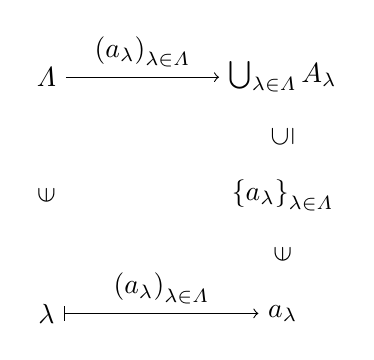
\begin{tikzpicture}[auto] 

  \node (e) at (0, 0) {$\lambda $};
  \node (f) at (3, 0) {$a_{\lambda } $};
  \node (g) at (0, 3) {$\varLambda $};
  \node (h) at (3, 3) {$\bigcup_{\lambda \in \varLambda } A_{\lambda } $};
  \node[rotate=90] (m) at (0, 1.5) {$\in $};
  \node[rotate=90] (m) at (3, 0.75) {$\in $};
  \node (n) at (3, 1.5) {$\left\{ a_{\lambda } \right\}_{\lambda \in \varLambda } $};
  \node[rotate=90] (o) at (3, 2.25) {$\subseteq $};
  \draw [|->] (e) to node {$\left( a_{\lambda } \right)_{\lambda \in \varLambda } $} (f);
  \draw [->] (g) to node {$\left( a_{\lambda } \right)_{\lambda \in \varLambda } $} (h);

\end{tikzpicture}
\end{center}
\end{dfn}
\begin{dfn}
次式で定義される集合$\prod_{\lambda \in \varLambda} A_{\lambda}$を空でない集合$\varLambda$によって添数づけられた集合$\left\{ A_{\lambda} \right\}_{\lambda \in \varLambda}$の一般化された直積という。なお、集合$\mathfrak{F}\left( \varLambda,\bigcup_{\lambda \in \varLambda} A_{\lambda} \right)$に属し、$\forall\lambda \in \varLambda$に対し、$f(\lambda) \in A_{\lambda}$なる写像$f$を用いた集合$f(\lambda)$を$a_{\lambda}$とおいた。
\begin{align*}
\prod_{\lambda \in \varLambda} A_{\lambda} = \left\{ f \in \mathfrak{F}\left( \varLambda,\bigcup_{\lambda \in \varLambda} A_{\lambda} \right) \middle| \forall\lambda \in \varLambda\left[ f(\lambda) \in A_{\lambda} \right] \right\}
\end{align*}
その写像$f$は次式のようにも書かれることができる。
\begin{center}
\begin{tikzpicture}[auto] 
  
  \node (i) at (0, 0) {$\lambda $};
  \node (j) at (3, 0) {$f \left( \lambda \right) $};
  \node (k) at (0, 3) {$\varLambda $};
  \node (l) at (3, 3) {$\bigcup_{\lambda \in \varLambda } A_{\lambda } $};
  \node[rotate=90] (m) at (0, 1.5) {$\in $};
  \node[rotate=90] (m) at (3, 0.75) {$\in $};
  \node[rotate=90] (o) at (3, 2.25) {$\subseteq $};
  \node (p) at (3, 1.5) {$A_{\lambda } $};
  \draw [|->] (i) to node {$f$} (j);
  \draw [->] (k) to node {$f$} (l);
  
\end{tikzpicture}
\end{center}
\end{dfn}
このとき、$f \in \prod_{\lambda \in \varLambda} A_{\lambda}$が成り立つならそのときに限り、写像$f:\varLambda \rightarrow \bigcup_{\lambda \in \varLambda} A_{\lambda}$が与えられ、$\forall\lambda \in \varLambda$に対し、$f(\lambda) \in A_{\lambda}$が成り立つのであった。これにより、その写像$f$はその集合$\bigcup_{\lambda \in \varLambda} A_{\lambda}$のその添数集合$\varLambda$によって順序づけられた組となっている。
\begin{dfn}
特に、集合$A$が与えられたとき、添数集合$\varLambda$によって添数づけられたその集合$\mathfrak{P}(A)$の集合族$\left\{ a_{\lambda} \right\}_{\lambda \in \varLambda}$をその集合$A$の部分集合族などという。もちろん、$\varLambda = \mathbb{N}$が成り立つなら、その集合$A$の写像$\left( a_{\lambda} \right)_{\lambda \in \varLambda}$はその集合$A$の無限列であるし、$\varLambda = \varLambda_{n}$が成り立つなら、その集合$A$の写像$\left( a_{\lambda} \right)_{\lambda \in \varLambda}$はその集合$A$の長さが$n$の有限列である。
\end{dfn}
\begin{dfn}
添数$\lambda$に依存しない集合$A$を用いた直積$\prod_{\lambda \in \varLambda_{n}} A$を$A^{n}$と書くことがある。
\end{dfn}
\begin{thm}\label{1.2.5.3}
添数集合$\varLambda$を用いた空集合でない直積$\prod_{\lambda \in \varLambda} A_{\lambda}$について、次式のような写像${\mathrm{pr}}_{\lambda}$が定義されるとき、
\begin{center}
\begin{tikzpicture}[auto] 

  \node (a) at (0, 0) {$\left( a_{\lambda } \right)_{\lambda \in \varLambda } $};
  \node (b) at (3, 0) {$a_{\lambda } $};
  \node (c) at (0, 3) {$\prod_{\lambda \in \varLambda } A_{\lambda } $};
  \node (d) at (3, 3) {$A_{\lambda } $};
  \node[rotate=90] (m) at (0, 1.5) {$\in $};
  \node[rotate=90] (m) at (3, 1.5) {$\in $};
  \draw [|->] (a) to node {${\rm pr}_{\lambda } $} (b);
  \draw [->] (c) to node {${\rm pr}_{\lambda } $} (d);

\end{tikzpicture}
\end{center}
このような写像${\mathrm{pr}}_{\lambda}$は存在する。
\end{thm}
\begin{proof}
添数集合$\varLambda$を用いた空集合でない直積$\prod_{\lambda \in \varLambda} A_{\lambda}$について、次式のような写像${\mathrm{pr}}_{\lambda'}$が定義されるとき、
\begin{align*}
{\mathrm{pr}}_{\lambda}:\prod_{\lambda \in \varLambda} A_{\lambda} \rightarrow A_{\lambda};\left( a_{\lambda} \right)_{\lambda \in \varLambda} \mapsto a_{\lambda}
\end{align*}
その直積$\prod_{\lambda \in \varLambda} A_{\lambda}$は空集合ではないので、$\forall\lambda \in \varLambda$に対し$A_{\lambda} \neq \emptyset$が成り立ち、したがって、$\forall\left( a_{\lambda} \right)_{\lambda \in \varLambda} \in \prod_{\lambda \in \varLambda} A_{\lambda}$に対し、その元$a_{\lambda}$がその集合$A_{\lambda}$に存在する。また、定義より明らかにその元$a_{\lambda}$は一意的である。
\end{proof}
\begin{dfn}
このような写像${\mathrm{pr}}_{\lambda}$をその直積$\prod_{\lambda \in \varLambda} A_{\lambda}$からその集合$A_{\lambda}$へのその添数$\lambda$における射影といい$\mathrm{proj}_{\lambda}$ともかく\footnote{ああいうminorだけど便利なヤツたまにあるんだよね(*`∀`)}。さらにここでは、記法上の都合上、$\mathrm{pr}_\lambda $をさらに$1_\lambda $とも書くことにする\footnote{ローカルルール注意です...。}。
\end{dfn}
\begin{dfn}
さらに、その添数$\lambda$における射影${\mathrm{pr}}_{\lambda}$によるその添数づけられたその集合$\bigcup_{\lambda \in \varLambda} A_{\lambda}$の集合族$\left\{ a_{\lambda} \right\}_{\lambda \in \varLambda}$の像$a_{\lambda}$をその順序づけられた組$\left( a_{\lambda} \right)_{\lambda \in \varLambda}$の$\lambda$成分、$\lambda$座標などという。
\end{dfn}
\subsubsection{$n$項演算}
\begin{dfn}
次式のように直積$\prod_{\lambda \in \varLambda} A_{\lambda}$から集合$B$への写像$f$が与えられたとする。
\begin{align*}
f:\prod_{\lambda \in \varLambda} A_{\lambda} \rightarrow B
\end{align*}
このとき、その直積$\prod_{\lambda \in \varLambda} A_{\lambda}$の任意の元は順序づけられた組$\left( a_{\lambda} \right)_{\lambda \in \varLambda}$となっているので、これのその写像$f$による像$f\left( \left( a_{\lambda} \right)_{\lambda \in \varLambda} \right)$を単に$f\left( a_{\lambda} \right)_{\lambda \in \varLambda}$と書く。
\end{dfn}
\begin{dfn}
ある集合たち$A$、$B$を用いた次式のような写像$f$が与えられたとき、その写像$f$は$n$項演算などという。
\begin{align*}
f:\prod_{\lambda \in \varLambda_{n}} A \rightarrow B
\end{align*}
特に、$n = 2$とした$n$項演算を単に演算、算法などという。
\end{dfn}
\begin{dfn}
さらに、誤解の恐れがないとき、写像$\rho :\prod_{\lambda \in \Lambda } B_{\lambda } \rightarrow V$と写像の族$\{f_{\lambda } :A_{\lambda } \rightarrow B_{\lambda } \}_{\lambda \in \varLambda }$が与えられたとき、次のように定義される写像$f$を$\rho \left(f_{\lambda } \right)_{\lambda \in \varLambda }$と略記する。
\begin{align*}
f:\prod_{\lambda \in \Lambda } A_{\lambda } \rightarrow V;\left( a_{\lambda } \right)_{\lambda \in \varLambda } \mapsto \rho \left(f_{\lambda } \left(a_{\lambda } \right) \right)_{\lambda \in \varLambda }
\end{align*}
\end{dfn}
\subsubsection{写像に関する一定理}
\begin{thm}\label{1.2.5.4}
写像$f:A \rightarrow B$において、次のことが成り立つ。
\begin{itemize}
\item
  その写像$f$が全射であるならそのときに限り、$f \circ g = I_{B}$が成り立つような写像$g:B \rightarrow A$が存在する。
\item
  その写像$f$が単射であるならそのときに限り、$g \circ f = I_{A}$が成り立つような写像$g:B \rightarrow A$が存在する。
\end{itemize}
\end{thm}
\begin{proof} 写像$f:A \rightarrow B$が与えられたとする。\par
$f \circ g = I_{B}$が成り立つような写像$g:B \rightarrow A$が存在するかつ、その写像$f$が全射でないと仮定しよう。このとき、$V(f) \subset B$が成り立つので、$b \in V(f) \setminus B$なる元$b$について、恒等写像の定義より$f \circ g(b) = I_{B}(b) = b \in V(f) \setminus B$が成り立つ。一方で、その対応$g$は写像であったので、$D(g) = B$が成り立ち、したがって、$g(b) \in A$が成り立つ。これにより、$f\left( g(b) \right) = f \circ g(b) \in V(f)$が成り立つことになるが、これは$f \circ g(b) \in V(f) \setminus B$が成り立つことに矛盾する。したがって、$f \circ g = I_{B}$が成り立つような写像$g:B \rightarrow A$が存在するなら、その写像$f$が全射である。\par
逆に、その写像$f$が全射であるとき、$V(f) = B$が成り立つので、$\forall b \in B$に対しその写像$f$のgraph$G$を用いて$(a,b) \in G$となる元$a$が存在する。したがって、$V\left( f^{- 1}|\left\{ b \right\} \right)$は空集合ではない。ここで、選択の公理よりその集合族$\left\{ V\left( f^{- 1}|\left\{ b \right\} \right) \right\}_{b \in B}$の選択写像を$c$とすれば、$V\left( f^{- 1}|\left\{ b \right\} \right)$は空集合ではないので、$c\left( V\left( f^{- 1}|\left\{ b \right\} \right) \right) \in V\left( f^{- 1}|\left\{ b \right\} \right)$が成り立つ。ここで、次式のような写像$g$を考えると、
\begin{align*}
g:B \rightarrow A;b \mapsto c\left( V\left( f^{- 1}|\left\{ b \right\} \right) \right)
\end{align*}
$\forall b \in B$に対し、$g(b) \in V\left( f^{- 1}|\left\{ b \right\} \right)$が成り立つので、$\left( g(b),b \right) \in G$が成り立ち$b \in V\left( f|\left\{ g(b) \right\} \right)$が成り立つ。ここで、その対応$f$は写像であったので、$V\left( f|\left\{ g(b) \right\} \right) = \left\{ b \right\}$が成り立ち、したがって、$f \circ g(b) = f\left( g(b) \right) = b = I_{B}(b)$が成り立つ。以上より、$\forall b \in B$に対し、$f \circ g(b) = I_{B}(b)$が成り立つので、$f \circ g = I_{B}$が成り立つような写像$g:B \rightarrow A$が存在する。\par
よって、その写像$f$が全射であるならそのときに限り、$f \circ g = I_{B}$が成り立つような写像$g:B \rightarrow A$が存在する。\par
$g \circ f = I_{A}$が成り立つような写像$g:B \rightarrow A$が存在するかつ、その写像$f$は単射でないと仮定しよう。このとき、$a \neq b$かつ$f(a) = f(b)$が成り立つような元々$a$、$b$がその集合$A$に存在することになる。したがって、恒等写像の定義より$g \circ f(a) = I_{A}(a) = a$かつ$g \circ f(b) = I_{A}(b) = b$が成り立つので、$g \circ f(a) \neq g \circ f(b)$が成り立つ。一方で、次式が成り立つが、
\begin{align*}
g \circ f(a) = g\left( f(a) \right) = g\left( f(b) \right) = g \circ f(b)
\end{align*}
これは$g \circ f(a) \neq g \circ f(b)$が成り立つことに矛盾する。したがって、次式が成り立つような写像$g:B \rightarrow A$が存在するなら、
\begin{align*}
g \circ f = I_{A}
\end{align*}
その写像$f$は単射である。\par
逆に、その写像$f$が単射であるとき、次式のような写像$f'$を考えると、
\begin{align*}
f':A \rightarrow V(f);a \mapsto f(a)
\end{align*}
その写像$f'$は全単射である。したがって、その写像$f'$の逆対応${f'}^{- 1}$は写像になる。ここで、$\forall a' \in A$に対し、次式のように写像$g$を定めると、
\begin{align*}
g:B \rightarrow A;b \mapsto \left\{ \begin{matrix}
{f'}^{- 1}(b) & {\mathrm{if}} & b \in V(f) \\
a' & {\mathrm{if}} & b \notin V(f) \\
\end{matrix} \right.\ 
\end{align*}
$\forall a \in A$に対し、$f(a) = f'(a) \in V(f)$が成り立つことに注意すれば、次のようになる。
\begin{align*}
g \circ f(a) = g\left( f(a) \right) = g\left( f'(a) \right) = {f'}^{- 1}\left( f'(a) \right) = {f'}^{- 1} \circ f'(a) = I_{A}(a) = a
\end{align*}
したがって、$g \circ f = I_{A}$が成り立つような写像$g:B \rightarrow A$が存在する。\par
よって、その写像$f$が単射であるならそのときに限り、$g \circ f = I_{A}$が成り立つような写像$g:B \rightarrow A$が存在する。
\end{proof}
\begin{thm}\label{1.2.5.5}
2つの集合たち$A$、$B$が与えられたとする。その集合$Aからその集合B$への単射が存在するならそのときに限り、その集合$Bからその集合A$への全射が存在する。
\end{thm}
\begin{proof}
2つの集合たち$A$、$B$が与えられたとする。単射$f:A \rightarrowtail B$が存在すらそのときに限り$g \circ f = I_{A}$が成り立つような写像$g:B \rightarrow A$が存在する。このような写像$f:A \rightarrow B$が存在するならそのときに限り、全射$g:B \twoheadrightarrow A$が存在する。
\end{proof}
\begin{thebibliography}{50}
  \bibitem{1}
    Rei Frontier Tech Blog. "ZFC公理系について:その1". Hatena Blog. \url{https://tech-blog.rei-frontier.jp/entry/2017/11/02/102042}, (2021-04-01 20:30 閲覧)
  \bibitem{2}
    Rei Frontier Tech Blog. "ZFC公理系について:その2". Hatena Blog. \url{https://tech-blog.rei-frontier.jp/entry/2017/11/09/100000}, (2021-04-01 20:30 閲覧)
  \bibitem{3}
    Rei Frontier Tech Blog. "ZFC公理系について:その3". Hatena Blog. \url{https://tech-blog.rei-frontier.jp/entry/2017/11/16/100000} (2021-04-01 20:30 閲覧)
  \bibitem{4}
    松坂和夫, 集合・位相入門, 岩波書店, 1968. 新装版第2刷 p39 ISBM978-4-00-029871-1
  \bibitem{5}
    WIIS. "写像による逆像". WIIS. \url{https://wiis.info/math/set/mapping/mapping-inverse-image/} (2021-2-27 15:30 閲覧)
  \bibitem{6}
    尾畑伸明. "第4章 写 像". 東北大学. \url{https://www.math.is.tohoku.ac.jp/~obata/student/subject/file/2018-4_shazo.pdf} (2021-2-27 15:45 閲覧)
\end{thebibliography}
\end{document}

\clearpage
\documentclass[dvipdfmx]{jsarticle}
\setcounter{section}{2}
\setcounter{subsection}{3}
\usepackage{amsmath,amsfonts,amssymb,array,comment,mathtools,url,docmute}
\usepackage{longtable,booktabs,dcolumn,tabularx,mathtools,multirow,colortbl,xcolor}
\usepackage[dvipdfmx]{graphics}
\usepackage{bmpsize}
\usepackage{amsthm}
\usepackage{enumitem}
\setlistdepth{20}
\renewlist{itemize}{itemize}{20}
\setlist[itemize]{label=•}
\renewlist{enumerate}{enumerate}{20}
\setlist[enumerate]{label=\arabic*.}
\setcounter{MaxMatrixCols}{20}
\setcounter{tocdepth}{3}
\newcommand{\rotin}{\text{\rotatebox[origin=c]{90}{$\in $}}}
\newcommand{\amap}[6]{\text{\raisebox{-0.7cm}{\begin{tikzpicture} 
  \node (a) at (0, 1) {$\textstyle{#2}$};
  \node (b) at (#6, 1) {$\textstyle{#3}$};
  \node (c) at (0, 0) {$\textstyle{#4}$};
  \node (d) at (#6, 0) {$\textstyle{#5}$};
  \node (x) at (0, 0.5) {$\rotin $};
  \node (x) at (#6, 0.5) {$\rotin $};
  \draw[->] (a) to node[xshift=0pt, yshift=7pt] {$\textstyle{\scriptstyle{#1}}$} (b);
  \draw[|->] (c) to node[xshift=0pt, yshift=7pt] {$\textstyle{\scriptstyle{#1}}$} (d);
\end{tikzpicture}}}}
\newcommand{\twomaps}[9]{\text{\raisebox{-0.7cm}{\begin{tikzpicture} 
  \node (a) at (0, 1) {$\textstyle{#3}$};
  \node (b) at (#9, 1) {$\textstyle{#4}$};
  \node (c) at (#9+#9, 1) {$\textstyle{#5}$};
  \node (d) at (0, 0) {$\textstyle{#6}$};
  \node (e) at (#9, 0) {$\textstyle{#7}$};
  \node (f) at (#9+#9, 0) {$\textstyle{#8}$};
  \node (x) at (0, 0.5) {$\rotin $};
  \node (x) at (#9, 0.5) {$\rotin $};
  \node (x) at (#9+#9, 0.5) {$\rotin $};
  \draw[->] (a) to node[xshift=0pt, yshift=7pt] {$\textstyle{\scriptstyle{#1}}$} (b);
  \draw[|->] (d) to node[xshift=0pt, yshift=7pt] {$\textstyle{\scriptstyle{#2}}$} (e);
  \draw[->] (b) to node[xshift=0pt, yshift=7pt] {$\textstyle{\scriptstyle{#1}}$} (c);
  \draw[|->] (e) to node[xshift=0pt, yshift=7pt] {$\textstyle{\scriptstyle{#2}}$} (f);
\end{tikzpicture}}}}
\renewcommand{\thesection}{第\arabic{section}部}
\renewcommand{\thesubsection}{\arabic{section}.\arabic{subsection}}
\renewcommand{\thesubsubsection}{\arabic{section}.\arabic{subsection}.\arabic{subsubsection}}
\everymath{\displaystyle}
\allowdisplaybreaks[4]
\usepackage{vtable}
\theoremstyle{definition}
\newtheorem{thm}{定理}[subsection]
\newtheorem*{thm*}{定理}
\newtheorem{dfn}{定義}[subsection]
\newtheorem*{dfn*}{定義}
\newtheorem{axs}[dfn]{公理}
\newtheorem*{axs*}{公理}
\renewcommand{\headfont}{\bfseries}
\makeatletter
  \renewcommand{\section}{%
    \@startsection{section}{1}{\z@}%
    {\Cvs}{\Cvs}%
    {\normalfont\huge\headfont\raggedright}}
\makeatother
\makeatletter
  \renewcommand{\subsection}{%
    \@startsection{subsection}{2}{\z@}%
    {0.5\Cvs}{0.5\Cvs}%
    {\normalfont\LARGE\headfont\raggedright}}
\makeatother
\makeatletter
  \renewcommand{\subsubsection}{%
    \@startsection{subsubsection}{3}{\z@}%
    {0.4\Cvs}{0.4\Cvs}%
    {\normalfont\Large\headfont\raggedright}}
\makeatother
\makeatletter
\renewenvironment{proof}[1][\proofname]{\par
  \pushQED{\qed}%
  \normalfont \topsep6\p@\@plus6\p@\relax
  \trivlist
  \item\relax
  {
  #1\@addpunct{.}}\hspace\labelsep\ignorespaces
}{%
  \popQED\endtrivlist\@endpefalse
}
\makeatother
\renewcommand{\proofname}{\textbf{証明}}
\usepackage{tikz,graphics}
\usepackage[dvipdfmx]{hyperref}
\usepackage{pxjahyper}
\hypersetup{
 setpagesize=false,
 bookmarks=true,
 bookmarksdepth=tocdepth,
 bookmarksnumbered=true,
 colorlinks=false,
 pdftitle={},
 pdfsubject={},
 pdfauthor={},
 pdfkeywords={}}
\begin{document}
%\hypertarget{ux5546ux96c6ux5408}{%
\subsection{商集合}%\label{ux5546ux96c6ux5408}}
\subsubsection{関係}%\label{ux95a2ux4fc2}}
\begin{dfn}
集合たち$A$、$B$が与えられたとする。このとき、$R = (A \times B,G):A \multimap B$なる対応$R$を考えると、その値域$V\left( R \middle| \left\{ a \right\} \right)$が空集合でないとき、対応の定義より次式が成り立つような元$b$がその集合$A$に存在する。
\begin{align*}
b \in V\left( R \middle| \left\{ a \right\} \right) \subseteq B
\end{align*}
このことを$aRb$と書きその対応$R$をその集合$A$からその集合$B$への関係といい、これのgraph$G$をその関係$R$のgraphといい$G(R)$とも書く。特に、$A = B$のとき、その関係$R$はその集合$A$における関係という。例えば、等号$=$、必要十分条件$\Leftrightarrow$などが挙げられる。
\end{dfn}
\begin{axs}
次のことを満たすような関係$R$をその集合$A$における同値関係という。
\begin{itemize}
\item
  その関係$R$は反射的である、即ち、$\forall a \in A$に対し、$aRa$が成り立つ。
\item
  その関係$R$は対称的である、即ち、$\forall a,b \in A$に対し、$aRb \Leftrightarrow bRa$が成り立つ。
\item
  その関係$R$は推移的である、即ち、$\forall a,b,c \in A$に対し、$aRb \land bRc \Rightarrow aRc$が成り立つ。
\end{itemize}
集合$A$における同値関係$R$が与えられたとき、$aRb$なるその集合$A$の2つの元々$a$、$b$はその同値関係$R$に関して同値であるという。
\end{axs}
\begin{axs}
次のことを満たすような関係$R$をその集合$A$における半順序関係、または単に、順序関係という。
\begin{itemize}
\item
  その関係$R$は反射的である、即ち、$\forall a \in A$に対し、$aRa$が成り立つ。
\item
  その関係$R$は反対称的である、即ち、$\forall a,b \in A$に対し、$aRb \land bRa \Rightarrow a = b$が成り立つ。
\item
  その関係$R$は推移的である、即ち、$\forall a,b,c \in A$に対し、$aRb \land bRc \Rightarrow aRc$が成り立つ。
\end{itemize}
\end{axs}
\begin{axs}
次のことを満たすような関係$R$をその集合$A$における全順序関係という。
\begin{itemize}
\item
  その関係$R$は反射的である、即ち、$\forall a \in A$に対し、$aRa$が成り立つ。
\item
  その関係$R$は反対称的である、即ち、$\forall a,b \in A$に対し、$aRb \land bRa \Rightarrow a = b$が成り立つ。
\item
  その関係$R$は推移的である、即ち、$\forall a,b,c \in A$に対し、$aRb \land bRc \Rightarrow aRc$が成り立つ。
\item
  その関係$R$は全順序的である、即ち、$\forall a,b \in A$に対し、$aRb \vee bRa$が成り立つ。
\end{itemize}
\end{axs}
\begin{thm}\label{1.2.5.6}
集合$A$から集合$B$への関係たち$R$、$S$が与えられたとき、$\forall a \in A\forall b \in B$に対し、$aRb \Leftrightarrow aSb$が成り立つならそのときに限り、$R = S$が成り立つ。
\end{thm}
\begin{proof}
集合$A$から集合$B$への関係たち$R$、$S$が与えられたとき、$\forall a \in A\forall b \in B$に対し、$aRb \Leftrightarrow aSb$が成り立つなら、次式が成り立つ。
\begin{align*}
b \in V\left( R|\left\{ a \right\} \right) \Leftrightarrow b \in V\left( S|\left\{ a \right\} \right)
\end{align*}
これはそれらの同値関係たち$R$、$S$のgraphsをそれぞれ$G(R)$、$G(S)$とおくと、次式のように書き換えられることができる。
\begin{align*}
b \in A \land \exists a' \in \left\{ a \right\}\left[ \left( a',b \right) \in G(R) \right] \Leftrightarrow b \in A \land \exists a' \in \left\{ a \right\}\left[ \left( a',b \right) \in G(S) \right]
\end{align*}
したがって、次のようになる。
\begin{align*}
&\quad \left( b \in A \land \exists a' \in \left\{ a \right\}\left[ \left( a',b \right) \in G(R) \right] \Leftrightarrow b \in A \land \exists a' \in \left\{ a \right\}\left[ \left( a',b \right) \in G(S) \right] \right)\\
&\Leftrightarrow \left( a,b \in A \land (a,b) \in G(R) \Leftrightarrow a,b \in A \land (a,b) \in G(S) \right)\\
&\Leftrightarrow \left( a,b \in A \land (a,b) \in G(R) \land (a,b) \in G(S) \right) \\
&\quad \vee \left( \neg a,b \in A \vee (a,b) \notin G(R) \vee (a,b) \notin G(S) \right)\\
&\Leftrightarrow \left( (a,b \in A \vee \neg a,b \in A) \land \left( \left( (a,b) \in G(R) \land (a,b) \in G(S) \right) \vee \neg a,b \in A \right) \right) \\
&\quad \vee \left( (a,b) \notin G(R) \vee (a,b) \notin G(S) \right)\\
&\Leftrightarrow \left( (a,b) \in G(R) \land (a,b) \in G(S) \right) \vee \left( (a,b) \notin G(R) \vee (a,b) \notin G(S) \right)\\
&\Leftrightarrow \left( (a,b) \in G(R) \Leftrightarrow (a,b) \in G(S) \right)
\end{align*}
これにより、$G(R) = G(S)$が成り立つので、$\left( A \times B,G(R) \right) = \left( A \times B,G(S) \right)$が成り立ち$R = S$が得られた。\par
逆に、$R = S$が成り立つなら、明らかに$\forall a \in A\forall b \in B$に対し、$aRb \Leftrightarrow aSb$が成り立つ。
\end{proof}
\begin{thm}\label{1.2.5.7}
ここで、写像$f:A \rightarrow B$が与えられたとする。このとき、その集合$A$の元々$a$、$b$に対し、次式のように論理式$aR(f)b$が定義されると、
\begin{align*}
aR(f)b \Leftrightarrow a,b \in A \land f(a) = f(b)
\end{align*}
その集合$A$における関係$R(f)$が得られこれは同値関係となる。
\end{thm}
\begin{dfn}
この関係$R(f)$をその写像$f$に付随する同値関係、その写像$f$の同値核などという。
\end{dfn}
\begin{proof}
写像$f:A \rightarrow B$が与えられたとする。このとき、その集合$A$の元々$a$、$b$に対し、次式のように論理式$aR(f)b$が定義されるとする。
\begin{align*}
aR(f)b \Leftrightarrow a,b \in A \land f(a) = f(b)
\end{align*}
このとき、次式のようなその集合$A \times A$の部分集合$G$が定義されると、
\begin{align*}
G = \left\{ (a,b) \in A^{2} \middle| f(a) = f(b) \right\}
\end{align*}
$R = (A,A,G):A \multimap A$なる対応$R$が得られ次のようになる。
\begin{align*}
aR(f)b &\Leftrightarrow a,b \in A \land f(a) = f(b)\\
&\Leftrightarrow b \in A \land a \in A \land (a,b) \in A^{2} \land f(a) = f(b)\\
&\Leftrightarrow b \in A \land a \in A \land (a,b) \in \left\{ (a,b) \in A^{2} \middle| f(a) = f(b) \right\}\\
&\Leftrightarrow b \in A \land a' \in \left\{ a \right\} \land \left( a',b \right) \in G\\
&\Leftrightarrow b \in A \land \exists a' \in \left\{ a \right\}\left[ \left( a',b \right) \in G \right]\\
&\Leftrightarrow b \in \left\{ b \in A \middle| \exists a' \in \left\{ a \right\}\left[ \left( a',b \right) \in G \right] \right\}\\
&\Leftrightarrow b \in V\left( R|\left\{ a \right\} \right) \Leftrightarrow aRb
\end{align*}
したがって、$aR(f)b \Leftrightarrow aRb$が得られる。したがって、その集合$A$における関係$R(f)$が得られている。\par
さらに、明らかに$\forall a \in A$に対し、明らかに$f(a) = f(a)$が成り立つので、$aR(f)a$が成り立つ。$\forall a,b \in A$に対し、$aR(f)b$が成り立つならそのときに限り、定義より明らかに$a,b \in A \land f(a) = f(b)$が成り立つ。これが成り立つならそのときに限り、やはり$bR(f)a$が成り立つので、$aR(f)b \Leftrightarrow bR(f)a$が成り立つ。$\forall a,b,c \in A$に対し、$aR(f)b \land bR(f)c$が成り立つならそのときに限り、定義より明らかに$f(a) = f(b) = f(c)$が成り立つ。したがって、$f(a) = f(c)$が成り立つので、やはり、$aR(f)c$が成り立つ。以上より、その関係$R(f)$が同値関係であることが示された。
\end{proof}
\begin{dfn}
その集合$\mathfrak{M}$に属する集合たち全体の和集合$\bigcup_{} \mathfrak{M}$のうち、$\forall A,B \in \mathfrak{M}$に対し、$A \cap B = \emptyset$が成り立つようなものをその集合$\mathfrak{M}$に属する集合たち全体の直和などといい$\bigsqcup_{A \in \mathfrak{M}} A$、$\bigsqcup_{} \mathfrak{M}$などと書く。
\end{dfn}
\begin{dfn}
集合$\mathfrak{M}$に属する集合たち全体の直和$\bigsqcup_{} \mathfrak{M}$が与えられたとき、集合$\mathfrak{M}$はその集合$\bigsqcup_{} \mathfrak{M}$の直和分割であるなどともいう。
\end{dfn}
\begin{thm}\label{1.2.5.8}
$\forall a \in \bigsqcup_{} \mathfrak{M}$に対し、$a \in A$なる集合$A$がその集合$\mathfrak{M}$に一意的に存在する。
\end{thm}
\begin{proof}
集合$\bigsqcup_{} \mathfrak{M}$の直和分割$\mathfrak{M}$が与えられたとき、$\forall a \in \bigsqcup_{} \mathfrak{M}$に対し、次式が成り立つので、
\begin{align*}
a \in \bigsqcup_{} \mathfrak{M} \Rightarrow a \in \bigcup_{} \mathfrak{M} \Leftrightarrow \exists A \in \mathfrak{M}[ a \in A]
\end{align*}
$a \in A$なる集合$A$がその集合$\mathfrak{M}$に存在する。ここで、その集合$A$とは異なる$a \in A'$なる集合$A'$がその集合$\mathfrak{M}$に存在すると仮定しよう。このとき、$a \in A$かつ$a \in A'$が成り立つので、$a \in A \cap A'$が成り立ちその集合$A \cap A'$は空集合ではない。しかしながら、$A,A'\in \mathfrak{M}$が成り立ち定義より$\forall A,B \in \mathfrak{M}$に対し、$A \cap B = \emptyset$が成り立つことに矛盾する。よって、このような集合$A'$は存在しない。
\end{proof}
\begin{thm}\label{1.2.5.9}
集合$\bigsqcup_{} \mathfrak{M}$の元々$a$、$b$に対し、次式のように論理式$aR_{\mathfrak{M}}b$が定義されると、
\begin{align*}
aR_{\mathfrak{M}}b \Leftrightarrow a \in A \land b \in B \land A,B \in \mathfrak{M \land}A = B
\end{align*}
その集合$\bigsqcup_{} \mathfrak{M}$における関係$R_{\mathfrak{M}}$が得られこれは同値関係となる。
\end{thm}
\begin{dfn}
この関係$R_{\mathfrak{M}}$をその直和分割$\mathfrak{M}$に付随する同値関係という。
\end{dfn}
このことは次のようにして考えられればわかりやすかろう。
\begin{center}
  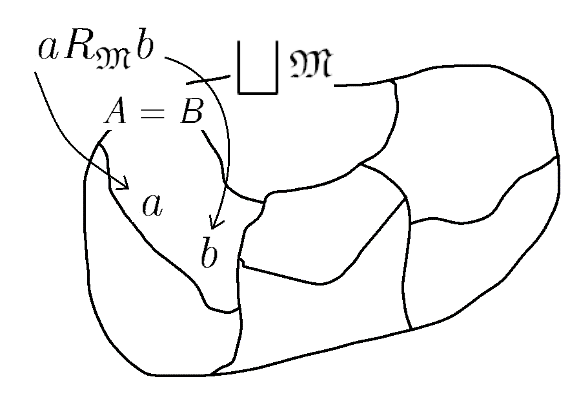
\includegraphics[width=160pt]{1.2.5.a.png}
\end{center}
\begin{proof}
集合$\bigsqcup_{} \mathfrak{M}$の直和分割$\mathfrak{M}$が与えられたとき、その集合$\bigsqcup_{} \mathfrak{M}$の元々$a$、$b$に対し、次式のように論理式$aR_{\mathfrak{M}}b$が定義されるとする。
\begin{align*}
aR_{\mathfrak{M}}b \Leftrightarrow a \in A \land b \in B \land A,B \in \mathfrak{M \land}A = B
\end{align*}
このとき、次式のようなその集合$\bigsqcup_{} \mathfrak{M} \times \bigsqcup_{} \mathfrak{M}$の部分集合$G$が定義されると、
\begin{align*}
G = \left\{ u \in \bigsqcup_{} \mathfrak{M} \times \bigsqcup_{} \mathfrak{M} \middle| u \in A \times B \land A,B \in \mathfrak{M \land}A = B \right\}
\end{align*}
$R = \left( \bigsqcup_{} \mathfrak{M},\bigsqcup_{} \mathfrak{M},G \right):\bigsqcup_{} \mathfrak{M} \multimap \bigsqcup_{} \mathfrak{M}$なる対応$R$が得られ$\forall a,b \in \bigsqcup_{} \mathfrak{M}$に対し、次のようになる。
\begin{align*}
aR_{\mathfrak{M}}b &\Leftrightarrow a \in A \land b \in B \land A,B \in \mathfrak{M \land}A = B\\
&\Leftrightarrow b \in B \land a \in A \land (a,b) \in A \times B \subseteq \bigsqcup_{} \mathfrak{M} \times \bigsqcup_{} \mathfrak{M} \\
&\quad \land A,B \in \mathfrak{M \land}A = B\\
&\Leftrightarrow b \in B \land a \in A \\
&\quad \land (a,b) \in \left\{ u \in \bigsqcup_{} \mathfrak{M} \times \bigsqcup_{} \mathfrak{M} \middle| u \in A \times B \land A,B \in \mathfrak{M} \land A = B \right\}\\
&\Leftrightarrow b \in B \land a' \in \left\{ a \right\} \land \left( a',b \right) \in G\\
&\Leftrightarrow b \in B \land \exists a' \in \left\{ a \right\}\left[ \left( a',b \right) \in G \right]\\
&\Leftrightarrow b \in \left\{ b \in B \middle| \exists a' \in \left\{ a \right\}\left[ \left( a',b \right) \in G \right] \right\}\\
&\Leftrightarrow b \in V\left( R|\left\{ a \right\} \right) \Leftrightarrow aRb
\end{align*}
したがって、$\forall a,b \in \bigsqcup_{} \mathfrak{M}$に対し、$aR_{\mathfrak{M}}b \Leftrightarrow aRb$が得られ$R_{\mathfrak{M}} = R$が成り立つ。したがって、その集合$\bigsqcup_{} \mathfrak{M}$における関係$R_{\mathfrak{M}}$が得られている。\par
さらに、$\forall a \in \bigsqcup_{} \mathfrak{M}$に対し、$a \in A$なる集合$A$がその集合$\mathfrak{M}$に一意的に存在するのであったので、次式が成り立つ。
\begin{align*}
a \in A \land a \in B \land A,B\in \mathfrak{M \land}A = B
\end{align*}
したがって、$aR_{\mathfrak{M}}a$が成り立つ。$\forall a,b \in \bigsqcup_{} \mathfrak{M}$に対し、$aR_{\mathfrak{M}}b$が成り立つならそのときに限り、次式が成り立つ。
\begin{align*}
a \in A \land b \in B \land A,B \in \mathfrak{M \land}A = B
\end{align*}
したがって、これが成り立つならそのときに限り、$bR_{\mathfrak{M}}a$が成り立ち$\forall a,b \in \bigsqcup_{} \mathfrak{M}$に対し、$aR_{\mathfrak{M}}b \Leftrightarrow bR_{\mathfrak{M}}a$が成り立つ。$\forall a,b,c \in \bigsqcup_{} \mathfrak{M}$に対し、$aR_{\mathfrak{M}}b$かつ$bR_{\mathfrak{M}}c$が成り立つならそのときに限り、次式が成り立つ。
\begin{align*}
a \in A \land b \in B \land c \in C \land A,B,C \in \mathfrak{M \land}A = B = C
\end{align*}
これが成り立つなら、次式が成り立つので、
\begin{align*}
a \in A \land c \in C \land A,C \in \mathfrak{M \land}A = C
\end{align*}
$aR_{\mathfrak{M}}c$が成り立ち$\forall a,b,c \in \bigsqcup_{} \mathfrak{M}$に対し、$aR_{\mathfrak{M}}b \land bR_{\mathfrak{M}}c \Rightarrow aR_{\mathfrak{M}}c$が成り立つ。以上より、その関係$R_{\mathfrak{M}}$が同値関係であることが示された。
\end{proof}
%\hypertarget{ux5546ux96c6ux5408-1}{%
\subsubsection{商集合}%\label{ux5546ux96c6ux5408-1}}
\begin{dfn}
集合$A$の1つの同値関係$R$が与えられたとする。このとき、次式のような集合$C_{R}(a)$が定義されよう。
\begin{align*}
C_{R}(a) = \left\{ c \in A \middle| aRc \right\} \subseteq A
\end{align*}
この集合$C_{R}(a)$をその同値関係$R$によるその元$a$の同値類、または単に、類などといい$[ a]_{R}$、$\overline{a}$などとも書く。
\end{dfn}\par
このことは次のようにして考えられればわかりやすかろう。
\begin{center}
  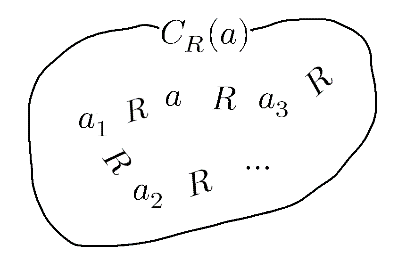
\includegraphics[width=160pt]{1.2.5.b.png}
\end{center}
\begin{thm}\label{1.2.5.10}
次のことが成り立つ。
\begin{itemize}
\item
  $\forall a \in A$に対し、$a \in C_{R}(a)$が成り立つ。
\item
  $\forall a,b \in A$に対し、$aRb$が成り立つならそのときに限り、$C_{R}(a) = C_{R}(b)$が成り立つ。
\item
  $\forall a,b \in A$に対し、$C_{R}(a) \neq C_{R}(b)$が成り立つなら、$C_{R}(a) \cap C_{R}(b) = \emptyset$が成り立つ。
\end{itemize}
\end{thm}
\begin{proof}
集合$A$の1つの同値関係$R$が与えられたとする。\par
$\forall a \in A$に対し、$a \in A$かつ$aRa$が成り立つので、$a \in \left\{ c \in A \middle| aRc \right\}$が成り立ち、したがって、$a \in C_{R}(a)$が成り立つ。\par
$\forall a,b \in A$に対し、$aRb$が成り立つならそのときに限り、$\forall c \in C_{R}(a)$に対し、定義より明らかに$c \in A$かつ$aRc$が成り立つ。ここで、$aRc$かつ$aRb$が成り立つので、これが成り立つなら、$bRc$が成り立つので、$c \in A$かつ$bRc$が成り立つ。これが成り立つならそのときに限り、$c \in C_{R}(b)$が成り立つので、次式が成り立つ。
\begin{align*}
c \in C_{R}(a) \Rightarrow c \in C_{R}(b)
\end{align*}
同様にして、次式が成り立つことが示される。
\begin{align*}
c \in C_{R}(b) \Rightarrow c \in C_{R}(a)
\end{align*}
これにより、外延性の公理より$C_{R}(a) = C_{R}(b)$が成り立つ。\par
逆に、$C_{R}(a) = C_{R}(b)$が成り立つならそのときに限り、$\forall c \in C_{R}(a)$に対し、次式が成り立つ。
\begin{align*}
c \in C_{R}(a) \Leftrightarrow c \in C_{R}(b)
\end{align*}
したがって、次のようになる。
\begin{align*}
\left( c \in C_{R}(a) \Leftrightarrow c \in C_{R}(b) \right) &\Leftrightarrow \left( c \in C_{R}(a) \land c \in C_{R}(b) \right) \\
&\quad \vee \left( c \notin C_{R}(a) \land c \notin C_{R}(b) \right)\\
&\Leftrightarrow (c \in A \land aRc \land bRc) \\
&\quad \vee \left( (c \notin A \vee \neg aRc) \land (c \notin A \vee \neg bRc) \right)\\
&\Leftrightarrow (c \in A \land aRc \land bRc) \vee c \notin A \vee (\neg aRc \land \neg bRc)\\
&\Leftrightarrow c \in A \land aRc \land bRc \Rightarrow aRb
\end{align*}
以上より、$\forall a,b \in A$に対し、$aRb$が成り立つならそのときに限り、$C_{R}(a) = C_{R}(b)$が成り立つ。\par
$\forall a,b \in A$に対し、$C_{R}(a) \neq C_{R}(b)$が成り立つかつ、$C_{R}(a) \cap C_{R}(b) \neq \emptyset$が成り立つと仮定しよう。このとき、上記の議論により$aRb$が成り立たないかつ、$c \in C_{R}(a) \cap C_{R}(b)$が成り立つような元$c$がその集合$A$に存在することになるので、次のようになる。
\begin{align*}
\neg aRb \land c \in C_{R}(a) \cap C_{R}(b) &\Leftrightarrow \neg aRb \land c \in A \land aRc \land bRc\\
&\Rightarrow aRc \land bRc \land \neg aRb\\
&\Rightarrow aRb \land \neg aRb \Leftrightarrow \bot
\end{align*}
これは矛盾している。したがって、$C_{R}(a) \neq C_{R}(b)$が成り立つなら、$C_{R}(a) \cap C_{R}(b) = \emptyset$が成り立つことが示された。
\end{proof}
\begin{thm}\label{1.2.5.11}
集合$A$の1つの同値関係$R$が与えられたとする。次式のようにその同値関係$R$によるその元$a$の同値類全体の集合$\mathfrak{M}$が定義されると、
\begin{align*}
\mathfrak{M}=\left\{ C_{R}(a)\in \mathfrak{P}(A) \middle| C_{R}(a) = \left\{ c \in A \middle| aRc \right\} \right\}
\end{align*}
その集合$\mathfrak{M}$はその集合$A$の直和分割でこれに付随する同値関係$R_{\mathfrak{M}}$はその同値関係$R$に等しい。
\end{thm}\par
このことは次のようにして考えられればわかりやすかろう。
\begin{center}
  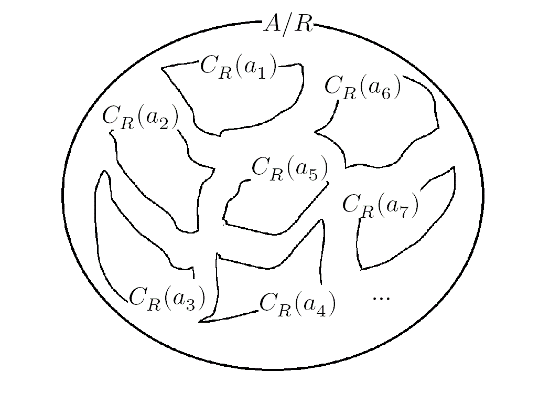
\includegraphics[width=160pt]{1.2.5.c.png}
\end{center}
\begin{proof}
集合$A$の1つの同値関係$R$が与えられたとする。次式のようにその同値関係$R$によるその元$a$の同値類全体の集合$\mathfrak{M}$が定義されるとき、
\begin{align*}
\mathfrak{M} =\left\{ C_{R}(a)\in \mathfrak{P}(A) \middle| C_{R}(a) = \left\{ c \in A \middle| aRc \right\} \right\}
\end{align*}
$\forall a \in A$に対し、$a \in C_{R}(a)$が成り立つので、$a \in C_{R}(a)\in \mathfrak{M}$なる集合$C_{R}(a)$が必ず存在する。したがって、次式が成り立つ。
\begin{align*}
a \in A \Leftrightarrow a \in C_{R}(a)\in \mathfrak{M} \Leftrightarrow \exists A'\in \mathfrak{M}\left[ a \in A' \right]
\end{align*}
したがって、次式が成り立つ。
\begin{align*}
A = \bigcup_{} \mathfrak{M}
\end{align*}\par
さらに、$\forall a,b \in A$に対し、$C_{R}(a) \neq C_{R}(b)$が成り立つなら、$C_{R}(a) \cap C_{R}(b) = \emptyset$が成り立つのであったので、$\forall A',B'\in \mathfrak{M}$に対し、$A' \neq B'$が成り立つなら、$A' \cap B' = \emptyset$が成り立つ。したがって、次式が成り立つ。
\begin{align*}
A = \bigsqcup_{} \mathfrak{M}
\end{align*}\par
さらに、$\forall a,b \in A$に対し、$aRb$が成り立つならそのときに限り、$C_{R}(a) = C_{R}(b)$が成り立つかつ、$\forall a,b \in A$に対し、$a \in C_{R}(a)$かつ$b \in C_{R}(b)$が成り立つのであったので、次式が成り立つ。
\begin{align*}
a \in C_{R}(a) \land b \in C_{R}(b) \land C_{R}(a) = C_{R}(b)
\end{align*}
また、その集合$\mathfrak{M}$の定義より明らかに$C_{R}(a),C_{R}(b)\in \mathfrak{M}$が成り立つので、次式が成り立つ。
\begin{align*}
a \in C_{R}(a) \land b \in C_{R}(b) \land C_{R}(a),C_{R}(b)\in \mathfrak{M \land}C_{R}(a) = C_{R}(b)
\end{align*}
これにより、その直和分割$\mathfrak{M}$に付随する同値関係$R_{\mathfrak{M}}$の定義より$aR_{\mathfrak{M}}b$が成り立つ。\par
以上より、$\forall a,b \in A$に対し、次式が成り立つので、
\begin{align*}
aRb \Leftrightarrow aR_{\mathfrak{M}}b
\end{align*}
$R = R_{\mathfrak{M}}$が得られた。
\end{proof}
\begin{dfn}
このようにして、その同値関係$R$からその集合$\mathfrak{M}$が定義されること、即ち、その集合$A$がその同値関係$R$によって得られる同値類たちの直和$\bigsqcup_{} \mathfrak{M}$とみなすことをその集合$A$のその同値関係$R$による類別、分類といいその集合$\mathfrak{M}$をその集合$A$のその同値関係による商集合といい$A/R$などと書く\footnote{こんなのいつどこで使うんだよって感じですが、これがないと整数や有理数が作れなくなっちゃうんですよ~。}。
\end{dfn}
%\hypertarget{ux6a19ux6e96ux7684ux5168ux5c04}{%
\subsubsection{標準的全射}%\label{ux6a19ux6e96ux7684ux5168ux5c04}}
\begin{thm}\label{1.2.5.12}
集合$A$の1つの同値関係$R$が与えられたとする。次式のように写像$C_{R}$が定義されるとき、
\begin{align*}
C_{R}:A \rightarrow A/R;a \mapsto C_{R}(a)
\end{align*}
その写像$C_{R}$は全射でありこれに付随する同値関係$R\left( C_{R} \right)$はその同値関係$R$に等しい。
\end{thm}
\begin{dfn}
このような写像$C_{R}$をその集合$A$からその集合$A/R$への標準的全射、自然な全射、商写像などという。
\end{dfn}
\begin{proof}
集合$A$の1つの同値関係$R$が与えられたとする。次式のように写像$C_{R}$が定義されるとき、
\begin{align*}
C_{R}:A \rightarrow A/R;a \mapsto C_{R}(a)
\end{align*}
商集合の定義より、$\forall c \in A/R$に対し、$c = C_{R}(a)$となるような元$a$がその集合$A$に存在する。したがって、次式が成り立つ。
\begin{align*}
c \in A/R \land \exists a \in A\left[ c = C_{R}(a) \right]
\end{align*}
これにより、$c \in V\left( C_{R} \right)$が成り立つので、$A/R \subseteq V\left( C_{R} \right)$が成り立つ。また、値域の定義より明らかに$V\left( C_{R} \right) \subseteq A/R$が成り立つ以上より、$A/R = V\left( C_{R} \right)$が得られその写像$C_{R}$は全射となる。\par
また、その写像$C_{R}$に付随する同値関係$R\left( C_{R} \right)$において、$\forall a,b \in A$に対し、定義より明らかに次式が成り立つ。
\begin{align*}
aR\left( C_{R} \right)b \Leftrightarrow C_{R}(a) = C_{R}(b)
\end{align*}
ここで、$\forall a,b \in A$に対し、$aRb$が成り立つならそのときに限り、$C_{R}(a) = C_{R}(b)$が成り立つのであったので、$aR\left( C_{R} \right)b \Leftrightarrow aRb$が成り立ち、したがって、$R\left( C_{R} \right) = R$が成り立つ。
\end{proof}
%\hypertarget{ux5199ux50cfux306eux5206ux89e3}{%
\subsubsection{写像の分解}%\label{ux5199ux50cfux306eux5206ux89e3}}
\begin{thm}[写像の分解]\label{1.2.5.13}
写像$f:A \rightarrow B$とこれに付随するその集合$A$の同値関係$R(f)$が与えられたとき、写像$g$が次式のように定義される。
\begin{align*}
g:A/R(f)\rightarrow V(f);C_{R(f)}(a) \mapsto f(a)
\end{align*}
このとき、次のことが成り立つ。
\begin{itemize}
\item
  その写像$g$は全単射である。
\item
  その集合$A$からその集合$A/R(f)$への標準的全射$C_{R(f)}$とその写像$g$とその集合$V(f)からその集合Bへの標準的単射i$を用いれば、$f = i \circ g \circ C_{R(f)}$が成り立つ、即ち、次式が成り立つ。
\begin{center}
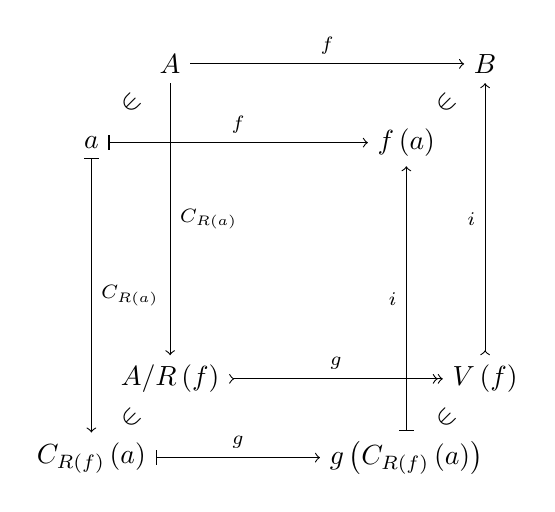
\begin{tikzpicture}[auto] 

  \node (a) at (1, 1) {$A/R\left( f\right) $};
  \node (b) at (5, 1) {$V\left( f\right) $};
  \node (c) at (0, 0) {$C_{R\left( f\right) } \left( a\right) $};
  \node (d) at (4, 0) {$g\left( C_{R\left( f\right) } \left( a\right) \right) $};
  \node (f) at (1, 5) {$A$};
  \node (g) at (5, 5) {$B$};
  \node (h) at (0, 4) {$a$};
  \node (i) at (4, 4) {$f\left( a\right) $};
  \node (e) at (0.5, 4.5) {\rotatebox{45}{$\in $} };
  \node (e) at (4.5, 4.5) {\rotatebox{45}{$\in $} };
  \node (e) at (0.5, 0.5) {\rotatebox{45}{$\in $} };
  \node (e) at (4.5, 0.5) {\rotatebox{45}{$\in $} };
    
  \draw [->] (f) to node {$\scriptstyle C_{R\left( a\right) } $} (a);
  \draw [>->>] (a) to node {$\scriptstyle g$} (b);
  \draw [>->] (b) to node {$\scriptstyle i$} (g);
  \draw [->] (f) to node {$\scriptstyle f$} (g);
  \draw [|->] (h) to node {$\scriptstyle C_{R\left( a\right) } $} (c);
  \draw [|->] (c) to node {$\scriptstyle g$} (d);
  \draw [|->] (d) to node {$\scriptstyle i$} (i);
  \draw [|->] (h) to node {$\scriptstyle f$} (i);
  
\end{tikzpicture} 
\end{center}
\end{itemize}
その写像$g$を特にその写像$f$に付随する全単射ともいう。このようにして、その写像$f$がその写像$i \circ g \circ C_{R(f)}$に書き換えられることをその写像$f$の写像たち$C_{R(f)}$、$g$、$i$への分解などという\footnote{これは代数学とかでちょくちょく使うらしいです。}。
\end{thm}
\begin{proof}
写像$f:A \rightarrow B$とこれに付随するその集合$A$の同値関係$R(f)$が与えられたとき、写像$g$が次式のように定義される。
\begin{align*}
g:A/R(f)\rightarrow V(f);C_{R(f)}(a) \mapsto f(a)
\end{align*}
このとき、定義より明らかに$V(g) \subseteq V(f)$が成り立つ。ここで、、$\forall f(a) \in V(f)$に対し、値域の定義より$f(a) \in V(f)$なる元$a$がその集合$A$に存在する。この元$a$に対し、明らかに同値類$C_{R(f)}(a)$がその集合$A/R(f)$に存在することになるので、$f(a) = g\left( C_{R(f)}(a) \right)$なる同値類$C_{R(f)}(a)$がその集合$A/R(f)$に存在することになる。したがって、次式が成り立ち
\begin{align*}
f(a) \in V(f) \land \exists C_{R(f)}(a) \in A/R(f)\left[ f(a) = g\left( C_{R(f)}(a) \right) \right]
\end{align*}
値域の定義より$f(a) \in V(g)$が成り立つので、$V(f) \subseteq V(g)$が得られる。以上より、$V(g) = V(f)$が成り立つので、その写像$g$は全射である。また、$\forall C_{R(f)}(a),C_{R(f)}(b) \in A/R(f)$に対し、$C_{R(f)}(a) \neq C_{R(f)}(b)$が成り立つなら、$aR(f)b$が成り立たないので、その写像$f$に付随する同値関係の定義より$f(a) \neq f(b)$が成り立つ。したがって、$g\left( C_{R(f)}(a) \right) \neq g\left( C_{R(f)}(b) \right)$が成り立つことになるので、その写像$g$は単射である。以上より、その写像$g$は全単射であることが示された。\par
また、その集合$A$からその集合$A/R(f)$への標準的全射$C_{R(f)}$とその集合$V(f)$からその集合$B$への標準的単射$i$が与えられたとすれば、$\forall a \in A$に対し、次式が成り立つ。
\begin{align*}
i \circ g \circ C_{R(f)}(a) = i\left( g\left( C_{R(f)}(a) \right) \right) = i\left( f(a) \right) = f(a)
\end{align*}
したがって、その写像$f$はその集合$A$からその集合$A/R(f)$への標準的全射$C_{R(f)}$とその写像$g$とその集合$V(f)$からその集合$B$への標準的単射$i$を用いた次式を満たす。
\begin{align*}
f = i \circ g \circ C_{R(f)}
\end{align*}
\end{proof}
\begin{thebibliography}{50}
\bibitem{1}
  松坂和夫, 集合・位相入門, 岩波書店, 1968. 新装版第2刷 p39-60 ISBM978-4-00-029871-1
\end{thebibliography}
\end{document}

\clearpage
\documentclass[dvipdfmx]{jsarticle}
\setcounter{section}{2}
\setcounter{subsection}{4}
\usepackage{amsmath,amsfonts,amssymb,array,comment,mathtools,url,docmute}
\usepackage{longtable,booktabs,dcolumn,tabularx,mathtools,multirow,colortbl,xcolor}
\usepackage[dvipdfmx]{graphics}
\usepackage{bmpsize}
\usepackage{amsthm}
\usepackage{enumitem}
\setlistdepth{20}
\renewlist{itemize}{itemize}{20}
\setlist[itemize]{label=•}
\renewlist{enumerate}{enumerate}{20}
\setlist[enumerate]{label=\arabic*.}
\setcounter{MaxMatrixCols}{20}
\setcounter{tocdepth}{3}
\newcommand{\rotin}{\text{\rotatebox[origin=c]{90}{$\in $}}}
\newcommand{\amap}[6]{\text{\raisebox{-0.7cm}{\begin{tikzpicture} 
  \node (a) at (0, 1) {$\textstyle{#2}$};
  \node (b) at (#6, 1) {$\textstyle{#3}$};
  \node (c) at (0, 0) {$\textstyle{#4}$};
  \node (d) at (#6, 0) {$\textstyle{#5}$};
  \node (x) at (0, 0.5) {$\rotin $};
  \node (x) at (#6, 0.5) {$\rotin $};
  \draw[->] (a) to node[xshift=0pt, yshift=7pt] {$\textstyle{\scriptstyle{#1}}$} (b);
  \draw[|->] (c) to node[xshift=0pt, yshift=7pt] {$\textstyle{\scriptstyle{#1}}$} (d);
\end{tikzpicture}}}}
\newcommand{\twomaps}[9]{\text{\raisebox{-0.7cm}{\begin{tikzpicture} 
  \node (a) at (0, 1) {$\textstyle{#3}$};
  \node (b) at (#9, 1) {$\textstyle{#4}$};
  \node (c) at (#9+#9, 1) {$\textstyle{#5}$};
  \node (d) at (0, 0) {$\textstyle{#6}$};
  \node (e) at (#9, 0) {$\textstyle{#7}$};
  \node (f) at (#9+#9, 0) {$\textstyle{#8}$};
  \node (x) at (0, 0.5) {$\rotin $};
  \node (x) at (#9, 0.5) {$\rotin $};
  \node (x) at (#9+#9, 0.5) {$\rotin $};
  \draw[->] (a) to node[xshift=0pt, yshift=7pt] {$\textstyle{\scriptstyle{#1}}$} (b);
  \draw[|->] (d) to node[xshift=0pt, yshift=7pt] {$\textstyle{\scriptstyle{#2}}$} (e);
  \draw[->] (b) to node[xshift=0pt, yshift=7pt] {$\textstyle{\scriptstyle{#1}}$} (c);
  \draw[|->] (e) to node[xshift=0pt, yshift=7pt] {$\textstyle{\scriptstyle{#2}}$} (f);
\end{tikzpicture}}}}
\renewcommand{\thesection}{第\arabic{section}部}
\renewcommand{\thesubsection}{\arabic{section}.\arabic{subsection}}
\renewcommand{\thesubsubsection}{\arabic{section}.\arabic{subsection}.\arabic{subsubsection}}
\everymath{\displaystyle}
\allowdisplaybreaks[4]
\usepackage{vtable}
\theoremstyle{definition}
\newtheorem{thm}{定理}[subsection]
\newtheorem*{thm*}{定理}
\newtheorem{dfn}{定義}[subsection]
\newtheorem*{dfn*}{定義}
\newtheorem{axs}[dfn]{公理}
\newtheorem*{axs*}{公理}
\renewcommand{\headfont}{\bfseries}
\makeatletter
  \renewcommand{\section}{%
    \@startsection{section}{1}{\z@}%
    {\Cvs}{\Cvs}%
    {\normalfont\huge\headfont\raggedright}}
\makeatother
\makeatletter
  \renewcommand{\subsection}{%
    \@startsection{subsection}{2}{\z@}%
    {0.5\Cvs}{0.5\Cvs}%
    {\normalfont\LARGE\headfont\raggedright}}
\makeatother
\makeatletter
  \renewcommand{\subsubsection}{%
    \@startsection{subsubsection}{3}{\z@}%
    {0.4\Cvs}{0.4\Cvs}%
    {\normalfont\Large\headfont\raggedright}}
\makeatother
\makeatletter
\renewenvironment{proof}[1][\proofname]{\par
  \pushQED{\qed}%
  \normalfont \topsep6\p@\@plus6\p@\relax
  \trivlist
  \item\relax
  {
  #1\@addpunct{.}}\hspace\labelsep\ignorespaces
}{%
  \popQED\endtrivlist\@endpefalse
}
\makeatother
\renewcommand{\proofname}{\textbf{証明}}
\usepackage{tikz,graphics}
\usepackage[dvipdfmx]{hyperref}
\usepackage{pxjahyper}
\hypersetup{
 setpagesize=false,
 bookmarks=true,
 bookmarksdepth=tocdepth,
 bookmarksnumbered=true,
 colorlinks=false,
 pdftitle={},
 pdfsubject={},
 pdfauthor={},
 pdfkeywords={}}
\begin{document}
%\hypertarget{ux81eaux7136ux6570}{%
\subsection{自然数}%\label{ux81eaux7136ux6570}}
%\hypertarget{ux7121ux9650ux7cfbux8b5c}{%
\subsubsection{無限系譜}%\label{ux7121ux9650ux7cfbux8b5c}}
\begin{thm}\label{1.2.4.1}
集合$A$が無限系譜である、即ち、次式が成り立つことを
\begin{align*}
\emptyset \in A \land \forall a \in A\left[ a \in A \Rightarrow {\mathrm{suc} }a \in A \right]
\end{align*}
$A:\mathrm{infinite\ genealogy}$とおくと、$\exists A\in \mathcal{F}$に対し、$A:\mathrm{infinite\ genealogy}$が成り立つ。
\end{thm}
\begin{dfn}
この式が成り立つような空集合ではない集合$\mathcal{F}$を無限樹という。
\end{dfn}
\begin{proof}
集合$A$について無限の公理は次式のようになるのであった。
\begin{align*}
\exists A\in \mathcal{F}\left[ \emptyset \in A \land \forall a \in A\left[ a \in A \Rightarrow {\mathrm{suc} }a \in A \right] \right]
\end{align*}
したがって、$\emptyset \in A \land \forall a \in A\left[ a \in A \Rightarrow {\mathrm{suc} }a \in A \right]$を$A:\mathrm{infinite\ genealogy}$とおくと、
\begin{align*}
&\quad \exists A\in \mathcal{F}\left[ \emptyset \in A \land \forall a \in A\left[ a \in A \Rightarrow {\mathrm{suc} }a \in A \right] \right] \\ 
&\Leftrightarrow \exists A\in \mathcal{F}[ A:\mathrm{infinite\ genealogy}]\\
&\Leftrightarrow \bot \vee \exists A\in \mathcal{F}[ A:\mathrm{infinite\ genealogy}]\\
&\Leftrightarrow \exists A\in \mathcal{F}\left[ A\mathcal{\notin F} \right] \vee \exists A\in \mathcal{F}[ A:\mathrm{infinite\ genealogy}]\\
&\Leftrightarrow \exists A\in \mathcal{F}[ A:\mathrm{infinite\ genealogy}]
\end{align*}
以上より$\exists A\in \mathcal{F}$に対し、$A:\mathrm{infinite\ genealogy}$が成り立つ。
\end{proof}
\begin{thm}\label{1.2.4.2}
無限樹$\mathcal{F}$は存在する。
\end{thm}
\begin{proof}
無限の公理より無限系譜$A$が存在できる。ここで、$\mathcal{F} =\left\{ A \right\}$とおくと、明らかに$\exists A \in \left\{ A \right\}$に対し、$A:\mathrm{infinite\ genealogy}$が成り立つ。これは無限樹となっている。
\end{proof}
\begin{thm}\label{1.2.4.3}
無限系譜$A$を用いて次式のように対象$\widetilde{A}$が与えられるとする。ここで、冪集合の公理、分出の公理、無限の公理よりその対象$\widetilde{A}$は明らかに集合となっている。
\begin{align*}
\widetilde{A} = \left\{ A'\in \mathfrak{P}(A) \middle| A':\mathrm{infinite\ genealogy} \right\}
\end{align*}
このとき、この集合$\widetilde{A}$は無限樹となる。
\end{thm}
\begin{proof}
無限系譜$A$を用いて次式のように対象$\widetilde{A}$が与えられるとするとき、
\begin{align*}
\widetilde{A} = \left\{ A'\in \mathfrak{P}(A) \middle| A':\mathrm{infinite\ genealogy} \right\}
\end{align*}
$A \in \mathfrak{P}(A)$が成り立つかつ、無限系譜の定義よりその命題$A:\mathrm{infinite\ genealogy}$は真である。したがって、$\exists A \in \widetilde{A}$に対し、$A:\mathrm{infinite\ genealogy}$が成り立つ。
\end{proof}
\begin{thm}\label{1.2.4.4}
次式のように集合$\omega$が与えられるとする。
\begin{align*}
\omega = \bigcap_{} \widetilde{A}
\end{align*}
このとき、次のことが成り立つ。
\begin{itemize}
\item
  $\omega:\mathrm{infinite\ genealogy}$が成り立つ。
\item
  その集合$\omega$はその無限系譜$A$によらない。
\item
  その集合$\omega$は任意の無限系譜の部分集合となる。
\end{itemize}
\end{thm}
\begin{proof}
無限系譜$A$を用いて次式のように集合$\widetilde{A}$が与えられ
\begin{align*}
\widetilde{A} = \left\{ A'\in \mathfrak{P}(A) \middle| A':\mathrm{infinite\ genealogy} \right\}
\end{align*}
これを用いて次式のように集合$\omega_{A}$が与えられるとする。
\begin{align*}
\omega_{A} = \bigcap_{} \widetilde{A}
\end{align*}
このとき、$\forall A' \in \widetilde{A}$に対し、$\emptyset \in A'$が成り立つので、$\emptyset \in \omega_{A}$も成り立つ。\par
さらに、$\forall a \in \omega_{A}$に対し、$a \in \omega_{A}$が成り立つなら、$\forall A' \in \widetilde{A}$に対し、$a \in A'$が成り立ち、したがって、${\mathrm{suc} }a \in A'$も成り立つ。これにより、${\mathrm{suc} }a \in \omega_{A}$も成り立つ。以上より、$\omega_{A}:\mathrm{infinite\ genealogy}$が成り立つ。\par
ここで、$\omega_{A}\in \mathfrak{P}(A)$が成り立つかつ、$\omega_{A}:\mathrm{infinite\ genealogy}$が成り立つので、$\omega_{A} \in \widetilde{A}$が成り立つ。任意の無限系譜$B$が与えられたとき、$\emptyset \in A$かつ$\emptyset \in B$が成り立つので、$\emptyset \in A \cap B$が成り立つかつ、$a \in A \cap B$が成り立つなら、$a \in A$かつ$a \in B$が成り立ち、それらの集合たち$A$、$B$は無限系譜であったので、${\mathrm{suc} }a \in A$かつ${\mathrm{suc} }a \in B$が成り立つので、${\mathrm{suc} }a \in A \cap B$が成り立つ。以上より、$A \cap B:\mathrm{infinite\ genealogy}$が成り立つ。ここで、$\forall a \in \omega_{A}$に対し、次のようになり、
\begin{align*}
a \in \omega_{A} &\Leftrightarrow a \in \bigcap_{} \widetilde{A}\\
&\Leftrightarrow \forall A' \in \widetilde{A}\left[ a \in A' \right]\\
&\Leftrightarrow \forall A' \in \left\{ A'\in \mathfrak{P}(A) \middle| A':\mathrm{infinite\ genealogy} \right\}\left[ a \in A' \right]\\
&\Leftrightarrow A'\in \mathfrak{P}(A) \land A':\mathrm{infinite\ genealogy} \land a \in A'
\end{align*}
ここで、$\forall A'\in \mathfrak{P}(A \cap B)$に対し、$A' \subseteq A \cap B \subseteq A$が成り立つので、$A'\in \mathfrak{P}(A)$が成り立つので、次のようになる。
\begin{align*}
a \in \omega_{A} &\Rightarrow A'\in \mathfrak{P}(A \cap B) \land A':\mathrm{infinite\ genealogy} \land a \in A'\\
&\Leftrightarrow \forall A' \in \left\{ A'\in \mathfrak{P}(A \cap B) \middle| A':\mathrm{infinite\ genealogy} \right\}\left[ a \in A' \right]\\
&\Leftrightarrow \forall A' \in \widetilde{A \cap B}\left[ a \in A' \right]\\
&\Leftrightarrow a \in \bigcap_{} \widetilde{A \cap B}\\
&\Leftrightarrow a \in \omega_{A \cap B}
\end{align*}
したがって、$\omega_{A} \subseteq \omega_{A \cap B}$が成り立つ。また、$\forall a \in \omega_{A \cap B}\forall A' \in \widetilde{A}$に対し、$A' \subseteq A$が成り立つので、$A' \cap B \subseteq A \cap B$が成り立ち、$\emptyset \in A'$かつ$\emptyset \in B$が成り立つので、$\emptyset \in A' \cap B$が成り立つかつ、$a \in A' \cap B$が成り立つなら、$a \in A'$かつ$a \in B$が成り立ち、それらの集合たち$A'$、$B$は無限系譜であったので、${\mathrm{suc} }a \in A'$かつ${\mathrm{suc} }a \in B$が成り立つので、${\mathrm{suc} }a \in A' \cap B$が成り立つ。以上より、$A' \cap B:\mathrm{infinite\ genealogy}$が成り立ち、したがって、$A' \cap B \in \widetilde{A \cap B}$が成り立つ。ここで、$a \in \omega_{A \cap B} = \bigcap_{A' \in \widetilde{A \cap B}} A'$が成り立つので、$a \in A' \cap B$が成り立ち、$A' \cap B \subseteq A'$が成り立つので、$\forall A' \in \widetilde{A}$に対し、$a \in A'$が成り立ち、したがって、$a \in \bigcap_{} \widetilde{A} = \omega_{A}$が成り立つ。これにより、$\omega_{A \cap B} \subseteq \omega_{A}$が成り立つので、上記の議論により$\omega_{A} = \omega_{A \cap B}$が成り立つ。同様にして、$\omega_{B} = \omega_{A \cap B}$が成り立つ。したがって、任意の無限系譜たち$A$、$B$に対し、$\omega_{A} = \omega_{B}$が成り立つので、その集合$\omega_{A}$はその無限系譜$A$によらないことが示された。\par
以下、その集合$\omega_{A}$を$\omega$とおく。任意の無限系譜$B$が与えられたとき、$\forall a \in \omega$に対し、その集合$\omega$はその無限系譜$A$によらないので、次のようになり、
\begin{align*}
a \in \omega &\Leftrightarrow a \in \bigcap_{} \widetilde{B}\\
&\Leftrightarrow \forall B' \in \widetilde{B}\left[ a \in B' \right]\\
&\Leftrightarrow \forall B' \in \left\{ B'\in \mathfrak{P}(B) \middle| B':\mathrm{infinite\ genealogy} \right\}\left[ a \in B' \right]\\
&\Leftrightarrow B'\in \mathfrak{P}(B) \land B':\mathrm{infinite\ genealogy} \land a \in B'\\
&\Rightarrow a \in B
\end{align*}
したがって、$\omega \subseteq B$が成り立ちその集合$\omega$は任意の無限系譜$B$の部分集合となる。\par
以上より、次のことが示された。
\begin{itemize}
\item
  $\omega:\mathrm{infinite\ genealogy}$が成り立つ。
\item
  その集合$\omega$はその無限系譜$A$によらない。
\item
  その集合$\omega$は任意の無限系譜の部分集合となる。
\end{itemize}
\end{proof}
%\hypertarget{peanoux306eux516cux7406}{%
\subsubsection{Peanoの公理}%\label{peanoux306eux516cux7406}}
\begin{axs}[Peanoの公理]
ある集合$\mathcal{N}$が与えられたとする。これが次の公理たちを満たすとき、その集合$\mathcal{N \setminus}\left\{ \nu \right\}$は$\mathbb{N}$などと書きこれの元を自然数という。それらの公理たちのことをまとめてPeanoの公理といいその組$\left( \mathcal{N,}\nu,\sigma \right)$をPeano系などという。ただし、その集合$\mathcal{N}$を$\mathbb{N}$とおくときがあることに注意されたい。このような混乱を避けるために、その集合$\mathcal{N \setminus}\left\{ \nu \right\}$を$\mathbb{N}^{+}$、$\mathbb{Z}^{+}$、$\mathbb{Z}_{> 0}$などとその集合$\mathcal{N}$を$\mathbb{N}_{0}$、$\mathbb{Z}_{0}$、$\mathbb{Z}_{\geq 0}$などとおくときがある。
\begin{itemize}
\item
  写像$\sigma:\mathcal{N \rightarrow N}$が存在する。これを後者関数などという。
\item
  ある1つの元$\nu$が存在し$\nu\in \mathcal{N \setminus}V(\sigma)$を満たす。
\item
  その写像$\sigma$は単射である。
\item
  $\forall\mathcal{N}'\in \mathfrak{P}\left( \mathcal{N} \right)$に対し、$\nu \in \mathcal{N}'$が成り立つかつ、$\forall n \in \mathcal{N}$に対し、$n \in \mathcal{N}'$が成り立つなら、$\sigma(n) \in \mathcal{N}'$が成り立つとき、$\mathcal{N}' = \mathcal{N}$が成り立つ。
\end{itemize}
ここで、その元$\nu$を$0$と書きその写像$\sigma$によるこれの像$\sigma(0)$を$1$と書く。
\end{axs}
\begin{thm}\label{1.2.4.5}
無限系譜$A$を用いて次式のように集合$\widetilde{A}$が与えられ
\begin{align*}
\widetilde{A} = \left\{ A'\in \mathfrak{P}(A) \middle| A':\mathrm{infinite\ genealogy} \right\}
\end{align*}
これを用いて次式のように集合$\omega$が与えられるとすると、
\begin{align*}
\omega = \bigcap_{} \widetilde{A}
\end{align*}
その組$(\omega,\emptyset,suc)$はPeano系である。
\end{thm}
\begin{proof}
無限系譜$A$を用いて次式のように集合$\widetilde{A}$が与えられ
\begin{align*}
\widetilde{A} = \left\{ A'\in \mathfrak{P}(A) \middle| A':\mathrm{infinite\ genealogy} \right\}
\end{align*}
これを用いて次式のように集合$\omega$が与えられるとすると、
\begin{align*}
\omega = \bigcap_{} \widetilde{A}
\end{align*}
$\omega:\mathrm{infinite\ genealogy}$が成り立つので、次式のような写像$suc$が存在する。
\begin{align*}
suc:\omega \rightarrow \omega;a \mapsto a \cup \left\{ a \right\}
\end{align*}
ここで、次式が成り立つような元$a$がその集合$\omega$に存在すると仮定すると、
\begin{align*}
a \cup \left\{ a \right\} = \emptyset
\end{align*}
したがって、次のようになり
\begin{align*}
a = a' \Leftrightarrow a' \in \left\{ a \right\} \Rightarrow a' \in a \vee a' \in \left\{ a \right\} \Leftrightarrow a' \in a \cup \left\{ a \right\} = \emptyset
\end{align*}
空集合$\emptyset$に元が存在することになり空集合の公理に矛盾する。したがって、$\emptyset \in \omega \setminus V(suc)$が成り立つ。\par
$\forall\omega'\in \mathfrak{P}(\omega)$に対し、$\emptyset \in \omega'$かつ$\forall a \in \omega\left[ a \in \omega' \Rightarrow {\mathrm{suc} }a \in \omega' \right]$が成り立つなら、$\omega':\mathrm{infinite\ genealogy}$が成り立つ。ここで、その集合$\omega_{A}$は任意の無限系譜の部分集合となるのであったので、$\omega \subseteq \omega'$が成り立ち、したがって、$\omega = \omega'$が成り立つ。\par
$\forall a,b \in \omega$に対し、${\mathrm{suc} }a = {\mathrm{suc} }b$が成り立つとすると、$a \in \left\{ a \right\}$が成り立つことと正則性の公理より次式が成り立つ。
\begin{align*}
a \in {\mathrm{suc} }a = {\mathrm{suc} }b = b \cup \left\{ b \right\}
\end{align*}
これにより、$a = b$または$a \in b$が成り立つ。同様にして、$b = a$または$b \in a$が成り立つので、${\mathrm{suc} }a = {\mathrm{suc} }b \Rightarrow a = b \vee (a \in b \land b \in a)$が成り立つ。\par
ここで、$b = \emptyset$のとき、$a \in b$と$a \subset b$どちらも成り立たないので、$a \in b \Rightarrow a \subset b$と$a \subset b \Rightarrow a \in b$どちらも真となり$a \in b \Leftrightarrow a \subset b$が成り立つ。\par
$b \neq \emptyset$のとき、$\forall a \in \omega$に対し、$a \in \left\{ a \in \omega \middle| a \in b \Rightarrow a \subset b \right\}$が成り立つとき、これは次のようになる。
\begin{align*}
a \in \omega \land a \in b \Rightarrow a \subset b
\end{align*}
$a \in {\mathrm{suc} }b$が成り立つなら、${\mathrm{suc} }b = b \cup \left\{ b \right\}$より$a = b$または$a \in b$が成り立つ。\par
$a = b$が成り立つなら、$b \subseteq b \cup \left\{ b \right\}$が成り立つことに注意すれば、$a \subseteq {\mathrm{suc} }b$が成り立つ。ここで、$b = {\mathrm{suc} }b$が成り立つなら、${\mathrm{suc} }b = b \cup \left\{ b \right\}$より$b = b$または$b \in b$が成り立ち、したがって、$b \in b$が成り立つが、仮定の$b \in b \Rightarrow b \subset b$より、$b \neq b$となりこれは矛盾する。したがって、$b \neq {\mathrm{suc} }b$が成り立ち、したがって、$a \subset {\mathrm{suc} }b$が成り立つ。\par
$a \in b$が成り立つなら、仮定の$a \in b \Rightarrow a \subset b$より、$b \subseteq b \cup \left\{ b \right\}$が成り立つことに注意すれば、$a \subset {\mathrm{suc} }b$が成り立つ。\par
以上より、${\mathrm{suc} }b \in \left\{ a \in \omega \middle| a \in b \Rightarrow a \subset b \right\}$が成り立つので、上記の議論により$\omega = \left\{ a \in \omega \middle| a \in b \Rightarrow a \subset b \right\}$が成り立つ。\par
$b \neq \emptyset$のとき、$\forall a \in \omega$に対し、$a \in \left\{ a \in \omega \middle| a \subset b \Rightarrow a \in b \right\}$が成り立つとする。$a \subset {\mathrm{suc} }b$が成り立つなら、$b \in a$が成り立つと仮定すると、上記の議論により$b \in a \Rightarrow b \subset a$が成り立つので、次のようになるが、
\begin{align*}
b \subset a \vee a = b \Leftrightarrow b \subset a \vee \left\{ b \right\} = a \Rightarrow b \cup \left\{ b \right\} = {\mathrm{suc} }b \subseteq a
\end{align*}
これは仮定の$a \subset {\mathrm{suc} }b$が成り立つことに矛盾する。したがって、$b \notin a$が成り立つ。\par
このとき、仮定の$a \subset {\mathrm{suc} }b = b \cup \left\{ b \right\}$が成り立つことから、$b \in a$または$a \subseteq b$が成り立ち、上記の議論により$b \notin a$が成り立つので、$a \subseteq b$が成り立ち、したがって、$a \subset b$または$a = b$が成り立つ。ここで、$a \subset b$が成り立つなら、仮定の$a \subset b \Rightarrow a \in b$より$a \in b$が成り立つ。したがって、$a \in b$または$a = b$が成り立つ。これにより、次のようになる。
\begin{align*}
a \in b \vee a = b \Leftrightarrow a \in b \vee a \in \left\{ b \right\} \Leftrightarrow a \in b \cup \left\{ b \right\} = {\mathrm{suc} }b
\end{align*}
以上より、${\mathrm{suc} }b \in \left\{ a \in \omega \middle| a \subset b \Rightarrow a \in b \right\}$が成り立つので、上記の議論により$\omega = \left\{ a \in \omega \middle| a \subset b \Rightarrow a \in b \right\}$が成り立つ。\par
これにより、$a \in b$かつ$b \in a$が成り立つと仮定すると、先ほどの議論により次のようになり
\begin{align*}
a \in b \land b \in a \Leftrightarrow a \subset b \land b \subset a \Leftrightarrow \bot
\end{align*}
これは矛盾している。したがって、次のようになる。
\begin{align*}
{\mathrm{suc} }(a) = {\mathrm{suc} }b &\Rightarrow a = b \vee (a \in b \land b \in a)\\
&\Leftrightarrow a = b \vee \bot\\
&\Leftrightarrow a = b
\end{align*}
これにより、その写像$suc$は単射である。
\end{proof}
%\hypertarget{ux6570ux5b66ux7684ux5e30ux7d0dux6cd5ux306eux539fux7406}{%
\subsubsection{数学的帰納法の原理}%\label{ux6570ux5b66ux7684ux5e30ux7d0dux6cd5ux306eux539fux7406}}
\begin{thm}[数学的帰納法の原理]\label{1.2.4.6}
Peano系$\left( \mathcal{N,}\nu,\sigma \right)$が与えられたとする。その集合$\mathcal{N}$の元$n$に関する命題$\varphi(n)$について、次のことが成り立つなら、$\forall n \in \mathcal{N}$に対し、その命題$\varphi(n)$が成り立つ。$\nu \in \mathcal{N} \setminus V(\sigma)$なる元$\nu$を用いた命題$\varphi(\nu)$が成り立つ。
\begin{itemize}
\item
  $\forall k \in \mathcal{N}$に対し、命題$\varphi(k)$が成り立つなら、その後者関数$\sigma$を用いた命題$\varphi\left( \sigma(k) \right)$も成り立つ。
\end{itemize}\par
このことを数学的帰納法の原理などといいこれを用いてその命題$\varphi(n)$を示す方法を数学的帰納法という。
\end{thm}
\begin{proof}
Peano系$\left( \mathcal{N,}\nu,\sigma \right)$が与えられたとする。その集合$\mathcal{N}$の元$n$に関する命題$\varphi(n)$について、次のことが成り立つなら、
\begin{itemize}
\item
  $\nu \in \mathcal{N \setminus}V(\sigma)$なる元$\nu$を用いた命題$\varphi(\nu)$が成り立つ。
\item
  $\forall k \in \mathcal{N}$に対し、命題$\varphi(k)$が成り立つなら、その後者関数$\sigma$を用いた命題$\varphi\left( \sigma(k) \right)$も成り立つ。
\end{itemize}
分出の公理より次式のように集合$\mathcal{N}'$が定義されれば、
\begin{align*}
\mathcal{N}' = \left\{ n \in \mathcal{N} \middle| \varphi(n) \right\}
\end{align*}
明らかに$\nu \in \mathcal{N}'$が成り立つかつ、$\forall k \in \mathcal{N}$に対し、$k \in \mathcal{N}'$が成り立つなら、$\sigma(k) \in \mathcal{N}'$が成り立つので、$\mathcal{N} =\mathcal{N}'$が成り立つ。これにより、$\forall n \in \mathcal{N}$に対し、外延性の公理より次式が成り立つ。
\begin{align*}
n \in \mathcal{N} &\Leftrightarrow n \in \mathcal{N}'\\
&\Leftrightarrow n \in \left\{ n \in \mathcal{N} \middle| \varphi(n) \right\}\\
&\Leftrightarrow n \in \mathcal{N \land}\varphi(n)\\
&\Rightarrow \varphi(n)
\end{align*}
\end{proof}
%\hypertarget{peanoux7cfbux3068ux5f8cux7d99ux8005}{%
\subsubsection{Peano系と後継者}%\label{peanoux7cfbux3068ux5f8cux7d99ux8005}}
\begin{thm}\label{1.2.4.7}
Peano系$\left( \mathcal{N,}\nu,\sigma \right)$が与えられたとする。このとき、$\mathcal{N} =V(\sigma) \sqcup \left\{ \nu \right\}$が成り立つ。
\end{thm}
これは全ての自然数は後継者であることを意味する。これにより、その元$\nu$以外のその集合$\mathcal{N}$の任意の元$n$に対し、$n = \sigma\left( n' \right)$が成り立つようなその集合$\mathcal{N}$の元$n'$が存在することも注意しよう。
\begin{proof}
Peano系$\left( \mathcal{N,}\nu,\sigma \right)$が与えられたとする。このとき、$n \in V(\sigma) \cap \left\{ \nu \right\}$なる元$n$がその集合$\mathcal{N}$に存在すると仮定しその元$n$を$n'$とおくと、次のようになる。
\begin{align*}
n' \in V(\sigma) \cap \left\{ \nu \right\} &\Leftrightarrow n' \in V(\sigma) \land n' = \nu\\
&\Rightarrow \nu \in V(\sigma)
\end{align*}
しかしながら、これはPeanoの公理より$\nu \in \mathcal{N \setminus}V(\sigma)$が成り立つことに矛盾する。したがって、$V(\sigma) \cap \left\{ \nu \right\} = \emptyset$が成り立つ。また、$V(\sigma) \subseteq \mathcal{N}$かつ$\left\{ \nu \right\} \subseteq \mathcal{N}$が成り立つので、$V(\sigma) \sqcup \left\{ \nu \right\} \subseteq \mathcal{N}$が成り立つ。\par
次に、$\forall n \in \mathcal{N}$に対し、$n \in V(\sigma) \sqcup \left\{ \nu \right\}$が成り立つことを示そう。$n = \nu$のとき、明らかに$\nu \in V(\sigma) \sqcup \left\{ \nu \right\}$が成り立つ。$n = k$のとき、$k \in V(\sigma) \sqcup \left\{ \nu \right\}$が成り立つと仮定しよう。$n = \sigma(k)$のとき、$\sigma(k) \in V(\sigma)$が成り立つので、結局$\sigma(k) \in V(\sigma) \sqcup \left\{ \nu \right\}$が成り立つ。以上より、$\forall n \in \mathcal{N}$に対し、$n \in V(\sigma) \sqcup \left\{ \nu \right\}$が成り立つので、$\mathcal{N \subseteq}V(\sigma) \sqcup \left\{ \nu \right\}$が成り立つ。\par
よって、$\mathcal{N} =V(\sigma) \sqcup \left\{ \nu \right\}$が成り立つ。
\end{proof}
\begin{thm}\label{1.2.4.8}
$\mathcal{N \setminus}\left\{ \nu \right\} = V(\sigma)$が成り立つ。
\end{thm}
\begin{proof}
Peano系$\left( \mathcal{N,}\nu,\sigma \right)$が与えられたとする。このとき、$\mathcal{N} =V(\sigma) \sqcup \left\{ \nu \right\}$が成り立つのであった。したがって、次のようになる。
\begin{align*}
\mathcal{N \setminus}\left\{ \nu \right\} &= \left( V(\sigma) \sqcup \left\{ \nu \right\} \right) \setminus \left\{ \nu \right\}\\
&= V(\sigma) \setminus \left\{ \nu \right\} \cup \left\{ \nu \right\} \setminus \left\{ \nu \right\}\\
&= V(\sigma) \setminus \left\{ \nu \right\}
\end{align*}
ここで、明らかに$V(\sigma) \setminus \left\{ \nu \right\} \subseteq V(\sigma)$が成り立つかつ、Peanoの公理より$\nu \in \mathcal{N \setminus}V(\sigma)$が成り立ち$V(\sigma) \subseteq V(\sigma) \setminus \left\{ \nu \right\}$が成り立つので、$\mathcal{N \setminus}\left\{ \nu \right\} = V(\sigma)$が成り立つ。
\end{proof}
%\hypertarget{ux5199ux50cfux306eux518dux5e30ux7684ux5b9aux7fa9}{%
\subsubsection{写像の再帰的定義}%\label{ux5199ux50cfux306eux518dux5e30ux7684ux5b9aux7fa9}}
\begin{thm}[写像の再帰的定義]\label{1.2.4.9}
Peano系$\left( \mathcal{N,}\nu,\sigma \right)$が与えられたとする。任意の集合$A$とこれの元$a_{\nu}$と写像$F:\mathcal{N \times}A \rightarrow A$を用いて次式のように写像$f:\mathcal{N \rightarrow}A$が定義されると、その写像$f$は一意的に存在する。
\begin{align*}
\left\{ \begin{matrix}
f(\nu) = a_{\nu} \\
\forall n \in \mathcal{N}\left[ f \circ \sigma(n) = F\left( n,f(n) \right) \right] \\
\end{matrix} \right.\ 
\end{align*}
\end{thm}
このようにして写像が定義されるときがあり定義するにあたってのこの方法を写像の再帰的定義という。
\begin{proof}
Peano系$\left( \mathcal{N,}\nu,\sigma \right)$が与えられたとする。任意の集合$A$とこれの元$a_{\nu}$と写像$F:\mathcal{N \times}A \rightarrow A$を用いて、その集合$\mathcal{N \times}A$の部分集合$g$が$\left( \nu,a_{\nu} \right) \in g$かつ、$\forall(n,a) \in g$に対し、$\left( \sigma(n),\ \ F(n,a) \right) \in g$を満たすことを$g:\mathrm{reflexively\ graph}$とおき次式のように$g:\mathrm{reflexively\ graph}$なる集合$g$全体の集合$\mathcal{F}$が考えられるとする。
\begin{align*}
\mathcal{F} =\left\{ g \in \mathfrak{P}\left( \mathcal{N \times}A \right) \middle| g:\mathrm{reflexively\ graph} \right\}
\end{align*}
このとき、$\left( \nu,a_{\nu} \right)\in \mathcal{N \times}A$かつ、$\forall(n,a)\in \mathcal{N \times}A$に対し、$\sigma(n)\in \mathcal{N}$かつ$F \in A$が成り立つので、$\left( \sigma(n),F(n,a) \right)\in \mathcal{N \times}A$が成り立ち$\mathcal{N \times}A:\mathrm{reflexively\ graph}$が成り立つ。したがって、$\mathcal{N \times}A\in \mathcal{F}$が成り立つ。これにより、その集合$\mathcal{F}$は空集合でない。\par
ここで、$G \in \bigcap_{} \mathcal{F}$のように集合$G$が定義されると、明らかに、$G\in \mathcal{F}$が成り立つかつ、$\forall g\in \mathcal{F}$に対し、$G \subseteq g$が成り立つ。\par
次に$\forall n \in \mathcal{N}$に対し、$(n,a)$なる元$a$が集合$A$に存在することを示そう。$n = \nu$のとき、$G:\mathrm{reflexively\ graph}$が成り立つので、$\left( \nu,a_{\nu} \right) \in G$が成り立つ。ここで、$\left( \nu,a' \right) \in G$なる元$a'$が集合$A \setminus \left\{ a_{\nu} \right\}$に存在すると仮定しよう。$G' = G \setminus \left\{ \left( \nu,a_{\nu} \right) \right\}$なる集合$G'$が定義されるとする。$\left( \nu,a_{\nu} \right) \in G$かつ$a_{\nu} \neq a'$より$\left( \nu,a' \right) \in G'$が成り立ち、さらに、$\forall\left( n',a \right) \in G'$に対し、$\left( n',a \right) \in G$が成り立ち、$G:\mathrm{reflexively\ graph}$が成り立つので、$\left( \sigma\left( n' \right),F\left( n',a \right) \right) \in G$が成り立つ。ここで、$\nu \neq \sigma\left( n' \right)$が成り立つのであったので、$\left( \sigma\left( n' \right),F\left( n',a \right) \right) \neq \left( \nu,a_{\nu} \right)$が成り立ち$\left( \sigma\left( n' \right),F\left( n',a \right) \right) \in G'$が成り立つので、$G':\mathrm{reflexively\ graph}$が成り立つ。これにより、$G'\in \mathcal{F}$かつ$G' \subset G$が成り立つが、これは仮定の、$\forall g\in \mathcal{F}$に対し、$G \subseteq g$が成り立つことに矛盾する。したがって、$\left( \nu,a_{\nu} \right)$なる元$a_{\nu}$が集合$A$に一意的に存在する。\par
$n = k$のとき、$\left( k,a_{k} \right) \in G$なる元$a_{k}$が集合$A$に一意的に存在すると仮定しよう。$n = \sigma(k)$のとき、$G:\mathrm{reflexively\ graph}$が成り立つので、$\left( \sigma(k),F\left( k,a_{k} \right) \right) \in G$が成り立つ。ここで、$\left( \sigma(k),a' \right) \in G$なる元$a'$が集合$A \setminus \left\{ F\left( k,a_{k} \right) \right\}$に存在すると仮定しよう。$G' = G \setminus \left\{ \left( \sigma(k),F\left( k,a_{k} \right) \right) \right\}$なる集合$G'$が定義されるとする。$\left( \nu,a_{\nu} \right) \in G$かつ$\nu \neq \sigma(k)$より$\left( \nu,a' \right) \in G'$が成り立ち、さらに、$\forall\left( n',a \right) \in G'$に対し、$\left( n',a \right) \in G$が成り立ち、$G:\mathrm{reflexively\ graph}$が成り立つので、$\left( \sigma\left( n' \right),F\left( n',a \right) \right) \in G$が成り立つ。$n' = k$のとき、仮定の$\left( k,a_{k} \right) \in G$なる元$a_{k}$が集合$A$に一意的に存在するので、次式が成り立つかつ、
\begin{align*}
\left( \sigma\left( n' \right),F\left( n',a \right) \right) = \left( \sigma(k),F\left( k,a_{k} \right) \right) \in G
\end{align*}
$a' \neq F\left( k,a_{k} \right)$が成り立つ。したがって、$\left( \sigma\left( n' \right),a' \right) \neq \left( \sigma(k),F\left( k,a_{k} \right) \right)$が成り立ち$\left( \sigma\left( n' \right),\ \ F\left( n',a \right) \right) \in G'$が成り立つので、$G':\mathrm{reflexively\ graph}$が成り立つ。$n' \neq k$のとき、その写像$\sigma$は単射であったので、$\sigma\left( n' \right) \neq \sigma(k)$が成り立つ。したがって、$\left( \sigma\left( n' \right),F\left( n',a \right) \right) \neq \left( \sigma(k),F\left( k,a_{k} \right) \right)$が成り立ち$\left( \sigma\left( n' \right),F\left( n',a \right) \right) \in G'$が成り立つので、$G':\mathrm{reflexively\ graph}$が成り立つ。これにより、$G' \in \mathcal{F}$かつ$G' \subset G$が成り立つが、これは仮定の、$\forall g\in \mathcal{F}$に対し、$G \subseteq g$が成り立つことに矛盾する。したがって、$\left( \sigma(k),F\left( k,a_{k} \right) \right) \in G$なる元$F\left( k,a_{k} \right)$が集合$A$に一意的に存在する。\par
以上より、$\forall n \in \mathcal{N}$に対し、$(n,a) \in G$なる元$a$が集合$A$に一意的に存在する。ここで、対応$f = \left( \mathcal{N \times}A,G \right)\mathcal{:N \multimap}A$が考えられると、$\forall n \in \mathcal{N}$に対し、次式が成り立つかつ、
\begin{align*}
V\left( f|\left\{ n \right\} \right) = \left\{ a \in A \middle| \exists n' \in \left\{ n \right\}\left[ \left( n',a \right) \in G \right] \right\} = \left\{ a \in A \middle| (n,a) \in G \right\}
\end{align*}
$(n,a) \in G$なる元$a$が集合$A$に一意的に存在するので、次式が成り立つようなその集合$A$の元$a$が存在する。
\begin{align*}
V\left( f|\left\{ n \right\} \right) = \left\{ a \right\}
\end{align*}
これにより、その対応$f$は写像である。ここで、$V\left( f|\left\{ \nu \right\} \right) = \left\{ a \in A \middle| (\nu,a) \in G \right\}$が成り立つかつ、$G:\mathrm{reflexively\ graph}$が成り立つので、$V\left( f \middle| \left\{ \nu \right\} \right) = \left\{ a_{\nu} \right\}$が成り立ち$f(\nu) = a_{\nu}$が成り立つ。さらに、$\forall n \in \mathcal{N}$に対し、$V\left( f|\left\{ \sigma(n) \right\} \right) = \left\{ a \in A \middle| \left( \sigma(n),a \right) \in G \right\}$が成り立つかつ、$G:\mathrm{reflexively\ graph}$が成り立つので、$\left( \sigma(n),F\left( n,f(n) \right) \right) \in G$が成り立つので、$V\left( f \middle| \left\{ \sigma(n) \right\} \right) = \left\{ F\left( n,f(n) \right) \right\}$が成り立ち$f\left( \sigma(n) \right) = F\left( n,f(n) \right)$が成り立つ。これにより、その写像$f$は次式を満たす。
\begin{align*}
\left\{ \begin{matrix}
f(\nu) = a_{\nu} \\
\forall n \in \mathcal{N}\left[ f \circ \sigma(n) = F\left( n,f(n) \right) \right] \\
\end{matrix} \right.\ 
\end{align*}\par
2つの互いに異なる写像たち$f:\mathcal{N \rightarrow}A$、$g:\mathcal{N \rightarrow}A$が次式を満たすとき、
\begin{align*}
\left\{ \begin{matrix}
f(\nu) = a_{\nu} \\
\forall n \in \mathcal{N}\left[ f \circ \sigma(n) = F\left( n,f(n) \right) \right] \\
\end{matrix} \right.\ ,\ \ \left\{ \begin{matrix}
g(\nu) = a_{\nu} \\
\forall n \in \mathcal{N}\left[ g \circ \sigma(n) = F\left( n,g(n) \right) \right] \\
\end{matrix} \right.\ 
\end{align*}
$f = g$が成り立つことを示そう。$n = \nu$のとき、明らかに$f(\nu) = a_{\nu} = g(\nu)$が成り立つ。$n = k$のとき、$f(k) = g(k)$が成り立つと仮定しよう。$n = \sigma(k)$のとき、$\sigma(k) \neq \nu$が成り立つので、次のようになる。
\begin{align*}
f\left( \sigma(k) \right) = f \circ \sigma(k) = F\left( k,f(k) \right) = F\left( k,g(k) \right) = g \circ \sigma(k) = g\left( \sigma(k) \right)
\end{align*}
以上より、$\forall n \in \mathcal{N}$に対し、$f(n) = g(n)$が成り立ち、したがって、$f = g$が成り立つ。このとき、それらの写像たち$f$、$g$が互いに異なるという仮定に矛盾する。よって、次式のように写像$f:\mathcal{N \rightarrow}A$が定義されると、その写像$f$は一意的に存在する。
\begin{align*}
\left\{ \begin{matrix}
f(\nu) = a_{\nu} \\
\forall n \in \mathcal{N}\left[ f \circ \sigma(n) = F\left( n,f(n) \right) \right] \\
\end{matrix} \right.\ 
\end{align*}
\end{proof}
%\hypertarget{peanoux7cfbux9593ux306eux5199ux50cf}{%
\subsubsection{Peano系間の写像}%\label{peanoux7cfbux9593ux306eux5199ux50cf}}
\begin{thm}\label{1.2.4.10}
2つのPeano系たち$\left( \mathcal{M,}\mu,\sigma \right)$、$\left( \mathcal{N,}\nu,\tau \right)$が与えられたとする。このとき、次のことを満たす、
\begin{itemize}
\item
  $F(\mu) = \nu$が成り立つ。
\item
  $F \circ \sigma = \tau \circ F$が成り立つ。
\end{itemize}
即ち、次式が成り立つ全単射な写像$F\mathcal{:M \rightarrow N}$が一意的に存在する。
\begin{center}
\begin{tikzpicture}[auto] 

  \node (a) at (1, 1) {${\mathcal N} $};
  \node (b) at (5, 1) {${\mathcal N} $};
  \node (c) at (0, 0) {$\nu $};
  \node (d) at (4, 0) {$\tau \left( \nu \right) $};
  \node (e) at (8, 0) {$\cdots $};
  \node (f) at (1, 5) {${\mathcal M} $};
  \node (g) at (5, 5) {${\mathcal M} $};
  \node (h) at (0, 4) {$\mu $};
  \node (i) at (4, 4) {$\sigma \left( \mu \right) $};
  \node (j) at (8, 4) {$\cdots $};
  \node (k) at (0.5, 4.5) {\rotatebox{45}{$\in $} };
  \node (k) at (4.5, 4.5) {\rotatebox{45}{$\in $} };
  \node (k) at (0.5, 0.5) {\rotatebox{45}{$\in $} };
  \node (k) at (4.5, 0.5) {\rotatebox{45}{$\in $} };
  \node (l) at (9, 1) {$\cdots $};
  \node (m) at (9, 5) {$\cdots $};
  
  \draw [>->] (a) to node {$\scriptstyle \tau $} (b);
  \draw [>->] (f) to node {$\scriptstyle \sigma $} (g);
  \draw [>->>] (f) to node {$\scriptstyle F$} (a);
  \draw [>->>] (g) to node {$\scriptstyle F$} (b);
  \draw [|->] (c) to node {$\scriptstyle \tau $} (d);
  \draw [|->] (h) to node {$\scriptstyle \sigma $} (i);
  \draw [|->] (d) to node {$\scriptstyle \tau $} (e);
  \draw [|->] (i) to node {$\scriptstyle \sigma $} (j);
  \draw [|->] (h) to node {$\scriptstyle F$} (c);
  \draw [|->] (i) to node {$\scriptstyle F$} (d);
  \draw [>->] (b) to node {$\scriptstyle \tau $} (l);
  \draw [>->] (g) to node {$\scriptstyle \sigma $} (m);

\end{tikzpicture} 
\end{center}
\end{thm}
\begin{proof}
2つのPeano系たち$\left( \mathcal{M,}\mu,\sigma \right)$、$\left( \mathcal{N,}\nu,\tau \right)$が与えられたとする。\par
このとき、次のことを満たす写像$F\mathcal{:M \rightarrow N}$が定義されると、
\begin{itemize}
\item
  $F(\mu) = \nu$が成り立つ。
\item
  $F \circ \sigma = \tau \circ F$が成り立つ。
\end{itemize}
これは次のように書き換えられることができる。
\begin{align*}
\left\{ \begin{matrix}
F(\mu) = \nu \\
\forall m\in \mathcal{M}\left[ F \circ \sigma(m) = \tau \circ F(m) \right] \\
\end{matrix} \right.\ 
\end{align*}
これは明らかに写像の再帰的定義なので、その写像$F$は一意的に存在する。\par
ここで、$\forall n \in \mathcal{N}$に対し、$n \in V(F)$が成り立つことを示そう。$n = \nu$のとき、定義より明らかに$\nu \in V(F)$が成り立つ。$n = k$のとき、$k \in V(F)$が成り立つと仮定しよう。$n = \tau(k)$のとき、仮定より$k = F\left( k' \right)$とおくと、定義より次のようになる。
\begin{align*}
\tau(k) = \tau\left( F\left( k' \right) \right) = \tau \circ F\left( k' \right) = F \circ \sigma\left( k' \right) = F\left( \sigma\left( k' \right) \right)
\end{align*}
ここで、その元$\sigma\left( k' \right)$がその集合$\mathcal{M}$に存在するので、$\tau(k) \in V(F)$が成り立つ。\par
以上より、$\forall n \in \mathcal{N}$に対し、$n \in V(F)$が成り立つ。$V(F) \subseteq \mathcal{N}$が成り立つことに注意すれば、外延性の公理より$V(F) = \mathcal{N}$が成り立つので、その写像$F$は全射である。次に、$\forall n \in \mathcal{N}$に対し、$V(F) = \mathcal{N}$が成り立つのであったので、次式が成り立つような元々$m_{1}$、$m_{2}$がその集合$\mathcal{M}$に存在する。
\begin{align*}
n = F\left( m_{1} \right) = F\left( m_{2} \right)
\end{align*}\par
ここで、$\forall n \in \mathcal{N}$に対し、$n = F\left( m_{1} \right) = F\left( m_{2} \right) \Rightarrow m_{1} = m_{2}$が成り立つことを示そう。$n = \nu$のとき、$\nu = F\left( m_{1} \right) = F\left( m_{2} \right) \land m_{1} \neq m_{2}$が成り立つと仮定しよう。その写像$F$の定義より$F(\mu) = \nu$が成り立つのであったので、$F(m) = n$かつ$m \neq \mu$なるその集合$\mathcal{M}$の元$m$が存在し、$\mathcal{M \setminus}\left\{ \mu \right\} = V(\sigma)$が成り立つのであったので、$m = \sigma\left( m' \right)$なる元$m'$がその集合$\mathcal{M}$に存在する。したがって、次のようになる。
\begin{align*}
\nu = F(\mu) = F(m) = F\left( \sigma\left( m' \right) \right) = F \circ \sigma\left( m' \right)
\end{align*}
ここで、その写像$F$の定義より$F \circ \sigma\left( m' \right) = \tau \circ F\left( m' \right)$が成り立つので、次式が成り立つ。
\begin{align*}
\nu = \tau \circ F\left( m' \right) = \tau\left( F\left( m' \right) \right) \in V(\tau)
\end{align*}
しかしながら、これはPeanoの公理より$\nu \in \mathcal{N \setminus}V(\tau)$が成り立つことに矛盾する。したがって、$\nu = F\left( m_{1} \right) = F\left( m_{2} \right) \Rightarrow m_{1} = m_{2}$が成り立つ。$n = k$のとき、$k = F\left( m_{1} \right) = F\left( m_{2} \right) \Rightarrow m_{1} = m_{2}$が成り立つと仮定しよう。$n = \tau(k)$のとき、$\tau(k) = F\left( m_{1} \right) = F\left( m_{2} \right) \land m_{1} \neq m_{2}$が成り立つと仮定しよう。このとき、$m_{1} = \mu$のとき、その写像$F$の定義より$F(\mu) = \nu$が成り立つのであったので、$\tau(k) = F\left( m_{1} \right) = \nu$が成り立ち$\tau(k) = \nu \in V(\tau)$が成り立つが、これはPeanoの公理より$\nu \in \mathcal{N \setminus}V(\tau)$が成り立つことに矛盾する。したがって、$m_{1} \neq \mu$が成り立つ。$m_{2} = \mu$のときも同様にして示される。$m_{1} \neq \mu$かつ$m_{2} \neq \mu$が成り立つなら、$\mathcal{N \setminus}\left\{ \nu \right\} = V(\tau)$が成り立つのであったので、次式が成り立つような元々$m_{1}'$、$m_{2}'$がその集合$\mathcal{M}$に存在する。
\begin{align*}
m_{1} = \sigma\left( m_{1}' \right) \land m_{2} = \sigma\left( m_{2}' \right)
\end{align*}
したがって、
\begin{align*}
\tau(k) = F\left( m_{1} \right) = F\left( m_{2} \right) &\Leftrightarrow \tau(k) = F\left( \sigma\left( m_{1}' \right) \right) = F\left( \sigma\left( m_{2}' \right) \right)\\
&\Leftrightarrow \tau(k) = F \circ \sigma\left( m_{1}' \right) = F \circ \sigma\left( m_{2}' \right)\\
&\Leftrightarrow \tau(k) = \tau \circ F\left( m_{1}' \right) = \tau \circ F\left( m_{2}' \right)
\end{align*}
ここで、その写像$\tau$は単射であったので、次式が成り立つ。
\begin{align*}
k = F\left( m_{1}' \right) = F\left( m_{2}' \right)
\end{align*}
ここで、仮定より$k = F\left( m_{1}' \right) = F\left( m_{2}' \right) \Rightarrow m_{1}' = m_{2}'$が成り立つので、$m_{1}' = m_{2}'$が得られる。したがって、$m_{1} = \sigma\left( m_{1}' \right) = \sigma\left( m_{2}' \right) = m_{2}$が得られるが、これは$m_{1} \neq m_{2}$が成り立つことに矛盾する。したがって、$n = \tau(k)$のとき、$\tau(k) = F\left( m_{1} \right) = F\left( m_{2} \right) \Rightarrow m_{1} = m_{2}$が成り立つ。\par
以上より、$\forall n \in \mathcal{N}$に対し、$n = F\left( m_{1} \right) = F\left( m_{2} \right) \Rightarrow m_{1} = m_{2}$が成り立つので、その写像$F$は単射である。よって、その写像$F$は全単射となる。
\end{proof}
%\hypertarget{ux52a0ux6cd5}{%
\subsubsection{加法}%\label{ux52a0ux6cd5}}
\begin{dfn}
Peano系$\left( \mathcal{N,}\nu,\sigma \right)$が与えられたとする。次のような写像$+$が定義されるとき、その写像$+$を加法、足し算などといい像$+ (m,n)$をそれらの元々$m$、$n$の和といい$m + n$などと書く。
\begin{align*}
\left\{ \begin{matrix}
 + (m,\nu) = m \\
\forall n \in \mathcal{N}\left[ + \left( m,\sigma(n) \right) = \sigma\left( + (m,n) \right) \right] \\
\end{matrix} \right.\ 
\end{align*}
\end{dfn}
\begin{thm}\label{1.2.4.11}
そのような写像$+$は一意的に存在する。
\end{thm}
\begin{proof}
Peano系$\left( \mathcal{N,}\nu,\sigma \right)$が与えられたとする。$\forall m \in \mathcal{N}$に対し、次式のように写像$+_{m}\mathcal{:N \rightarrow N}$が定義されるとする。
\begin{align*}
\left\{ \begin{matrix}
 +_{m}(\nu) = m \\
\forall n \in \mathcal{N}\left[ +_{m}\left( \sigma(n) \right) = \sigma\left( +_{m}(n) \right) \right] \\
\end{matrix} \right.\ 
\end{align*}
これは明らかに写像の再帰的定義なので、その写像$+_{m}$は一意的に存在する。
\end{proof}
\begin{thm}\label{1.2.4.12}
次のことが成り立つ。特に、上から1つ目、2つ目の定理のことを加法の交換法則、加法の結合法則などという。
\begin{itemize}
\item
  $\forall m,n \in \mathcal{N}$に対し、$+ (m,n) = + (n,m)$が成り立つ。
\item
  $\forall l,m,n \in \mathcal{N}$に対し、$+ \left( + (l,m),n \right) = + \left( l, + (m,n) \right)$が成り立つ。
\item
  $\forall n \in \mathcal{N}$に対し、$+ \left( n,\sigma(\nu) \right) = + \left( \sigma(\nu),n \right) = \sigma(n)$が成り立つ。
\end{itemize}
\end{thm}
\begin{proof}
Peano系$\left( \mathcal{N,}\nu,\sigma \right)$が与えられたとする。$\forall m,n \in \mathcal{N}$に対し、$+ (m,n) = + (n,m)$が成り立つことを示そう。\par
$\forall m,n \in \mathcal{N}$に対し、$n = \nu$のとき、明らかに$+ (m,\nu) = m$が成り立つ。ここで、$m = \nu$のとき、明らかに$+ (m,n) = + (\nu,\nu) = + (n,m)$が成り立つ。$m = k$のとき、$+ (k,\nu) = + (\nu,k)$が成り立つと仮定しよう。$m = \sigma(k)$のとき、次式が成り立つ。
\begin{align*}
+ \left( \sigma(k),\nu \right) &= \sigma(k)\\
&= \sigma\left( + (k,\nu) \right)\\
&= \sigma\left( + (\nu,k) \right)\\
&= + \left( \nu,\sigma(k) \right)
\end{align*}
したがって、$n = \nu$のとき、$\forall m \in \mathcal{N}$に対し、$+ (m,\nu) = + (\nu,m)$が成り立つ。$n = k$のとき、$\forall m \in \mathcal{N}$に対し、$+ (m,k) = + (k,m)$が成り立つと仮定しよう。$n = \sigma(k)$のとき、$m = \nu$のとき、上記の議論により$+ \left( \nu,\sigma(k) \right) = + \left( \sigma(k),\nu \right)$が成り立つ。$m = l$のとき、$+ \left( l,\sigma(k) \right) = + \left( \sigma(k),l \right)$が成り立つと仮定しよう。$m = \sigma(l)$のとき、次のようになる。
\begin{align*}
+ \left( \sigma(l),\sigma(k) \right) &= \sigma\left( + \left( \sigma(l),k \right) \right)\\
&= \sigma\left( + \left( k,\sigma(l) \right) \right)\\
&= \sigma\left( \sigma\left( + (k,l) \right) \right)\\
&= \sigma\left( \sigma\left( + (l,k) \right) \right)\\
&= \sigma\left( + \left( l,\sigma(k) \right) \right)\\
&= \sigma\left( + \left( \sigma(k),l \right) \right)\\
&= + \left( \sigma(k),\sigma(l) \right)
\end{align*}
したがって、$n = \sigma(k)$のとき、$\forall m \in \mathcal{N}$に対し、$+ \left( m,\sigma(k) \right) = + \left( \sigma(k),m \right)$が成り立つ。以上より、$\forall m,n \in \mathcal{N}$に対し、$+ (m,n) = + (n,m)$が成り立つ。\par
$\forall l,m,n \in \mathcal{N}$に対し、$+ \left( + (l,m),n \right) = + \left( l, + (m,n) \right)$が成り立つことを示そう。$n = \nu$のとき、次のようになる。
\begin{align*}
+ \left( + (l,m),\nu \right) = + (l,m) = + \left( l, + (m,\nu) \right)
\end{align*}
したがって、$n = \nu$のとき、$\forall l,m \in \mathcal{N}$に対し、$+ \left( + (l,m),\nu \right) = + \left( l, + (m,\nu) \right)$が成り立つ。$n = k$のとき、$\forall l,m \in \mathcal{N}$に対し、$+ \left( + (l,m),k \right) = + \left( l, + (m,k) \right)$が成り立つと仮定しよう。$n = \sigma(k)$のとき、次のようになる。
\begin{align*}
+ \left( + (l,m),\sigma(k) \right) &= \sigma\left( + \left( + (l,m),k \right) \right) = \sigma\left( + \left( l, + (m,k) \right) \right)\\
&= + \left( l,\sigma\left( + (m,n) \right) \right) = + \left( l, + \left( m,\sigma(k) \right) \right)
\end{align*}
したがって、$n = \sigma(k)$のとき、$\forall l,m \in \mathcal{N}$に対し、$+ \left( + (l,m),\sigma(k) \right) = + \left( l, + \left( m,\sigma(k) \right) \right)$が成り立つ。以上より、$\forall l,m,n \in \mathcal{N}$に対し、$+ \left( + (l,m),n \right) = + \left( l, + (m,n) \right)$が成り立つ。\par
$\forall n \in \mathcal{N}$に対し、次式が成り立つ。
\begin{align*}
+ \left( n,\sigma(\nu) \right) = \sigma\left( + (n,\nu) \right) = \sigma(n)
\end{align*}
また、上記の議論により$+ \left( n,\sigma(\nu) \right) = + \left( \sigma(\nu),n \right)$が成り立つ。したがって、$\forall n \in \mathcal{N}$に対し、$+ \left( n,\sigma(\nu) \right) = + \left( \sigma(\nu),n \right) = \sigma(n)$が成り立つ。
\end{proof}
%\hypertarget{ux4e57ux6cd5}{%
\subsubsection{乗法}%\label{ux4e57ux6cd5}}
\begin{dfn}
Peano系$\left( \mathcal{N,}\nu,\sigma \right)$が与えられたとする。次のような写像$\cdot$が定義されるとき、その写像$\cdot$を乗法、掛け算などといい像$\cdot (m,n)$をそれらの元々$m$、$n$の積といい$m \cdot n$、$mn$、$m \times n$、$m*n$などと書く。
\begin{align*}
\left\{ \begin{matrix}
 \cdot (m,\nu) = \nu \\
\forall n \in \mathcal{N}\left[ \cdot \left( m,\sigma(n) \right) = + \left( \cdot (m,n),m \right) \right] \\
\end{matrix} \right.\ 
\end{align*}
\end{dfn}
\begin{thm}\label{1.2.4.13}
そのような写像$\cdot$は一意的に存在する。
\end{thm}
\begin{proof}
Peano系$\left( \mathcal{N,}\nu,\sigma \right)$が与えられたとする。$\forall m \in \mathcal{N}$に対し、次式のように写像$\cdot_{m}\mathcal{:N \rightarrow N}$が定義されるとする。
\begin{align*}
\left\{ \begin{matrix}
 \cdot_{m}(\nu) = \nu \\
\forall n \in \mathcal{N}\left[ \cdot_{m}\left( \sigma(n) \right) = + \left( \cdot_{m}(n),m \right) \right] \\
\end{matrix} \right.\ 
\end{align*}
これは明らかに写像の再帰的定義なので、その写像$\cdot_{m}$は一意的に存在する。
\end{proof}
\begin{thm}\label{1.2.4.14}
次のことが成り立つ。特に、上から1つ目、2つ目、3つ目の定理を乗法の交換法則、乗法の結合法則、乗法の加法に対する分配法則などという。
\begin{itemize}
\item
  $\forall m,n \in \mathcal{N}$に対し、$\cdot (m,n) = \cdot (n,m)$が成り立つ。
\item
  $\forall l,m,n \in \mathcal{N}$に対し、$\cdot \left( \cdot (l,m),n \right) = \cdot \left( l, \cdot (m,n) \right)$が成り立つ。
\item
  $\forall l,m,n \in \mathcal{N}$に対し、$\cdot \left( l, + (m,n) \right) = \cdot \left( + (m,n),l \right) = + \left( \cdot (l,m), \cdot (l,n) \right)$が成り立つ。
\item
  $\forall n \in \mathcal{N}$に対し、$\cdot \left( n,\sigma(\nu) \right) = \cdot \left( \sigma(\nu),n \right) = n$が成り立つ。
\end{itemize}
\end{thm}
\begin{proof}
Peano系$\left( \mathcal{N,}\nu,\sigma \right)$が与えられたとする。$\forall m,n \in \mathcal{N}$に対し、$\cdot (m,n) = \cdot (n,m)$が成り立つことを示そう。\par
$\forall m,n \in \mathcal{N}$に対し、$n = \nu$のとき、明らかに$\cdot (m,\nu) = \nu$が成り立つ。ここで、$m = \nu$のとき、明らかに$\cdot (m,\nu) = \nu = \cdot (\nu,m)$が成り立つ。$m = k$のとき、$\cdot (k,\nu) = \cdot (\nu,k)$が成り立つと仮定しよう。$m = \sigma(k)$のとき、次式が成り立つ。
\begin{align*}
\cdot \left( \sigma(k),\nu \right) = \nu = + \left( \cdot (\nu,k),\nu \right) = \cdot \left( \nu,\sigma(k) \right)
\end{align*}
したがって、$n = \nu$のとき、$\forall m \in \mathcal{N}$に対し、$\cdot (m,\nu) = \cdot (\nu,m)$が成り立つ。$n = k$のとき、$\forall m \in \mathcal{N}$に対し、$\cdot (m,k) = \cdot (k,m)$が成り立つと仮定しよう。$n = \sigma(k)$のとき、$m = \nu$のとき、上記の議論により$\cdot \left( \nu,\sigma(k) \right) = \cdot \left( \sigma(k),\nu \right)$が成り立つ。$m = l$のとき、$\cdot \left( l,\sigma(k) \right) = \cdot \left( \sigma(k),l \right)$が成り立つと仮定しよう。$m = \sigma(l)$のとき、次のようになる。
\begin{align*}
\cdot \left( \sigma(l),\sigma(k) \right) &= + \left( \cdot \left( \sigma(l),k \right),\sigma(l) \right)\\
&= + \left( \cdot \left( k,\sigma(l) \right), + \left( l,\sigma(\nu) \right) \right)\\
&= + \left( + \left( + \left( \cdot (k,l),k \right),l \right),\sigma(\nu) \right)\\
&= + \left( + \left( \cdot (l,k), + (k,l) \right),\sigma(\nu) \right)\\
&= + \left( + \left( \cdot (k,l),k \right), + \left( l,\sigma(\nu) \right) \right)\\
&= + \left( \cdot \left( k,\sigma(l) \right),\sigma(l) \right)\\
&= \cdot \left( \sigma(k),\sigma(l) \right)
\end{align*}
したがって、$n = \sigma(k)$のとき、$\forall m \in \mathcal{N}$に対し、$\cdot \left( m,\sigma(k) \right) = \cdot \left( \sigma(k),m \right)$が成り立つ。以上より、$\forall m,n \in \mathcal{N}$に対し、$\cdot (m,n) = \cdot (n,m)$が成り立つ。\par
$\forall l,m,n \in \mathcal{N}$に対し、$\cdot \left( l, + (m,n) \right) = + \left( \cdot (l,m), \cdot (l,n) \right)$が成り立つことを示そう。$l = \nu$のとき、次のようになる。
\begin{align*}
\cdot \left( \nu, + (m,n) \right) &= \cdot \left( + (m,n),\nu \right)\\
&= \nu = + (\nu,\nu)\\
&= + \left( \cdot (m,\nu), \cdot (n,\nu) \right)\\
&= + \left( \cdot (\nu,m), \cdot (\nu,n) \right)
\end{align*}
$l = k$のとき、$\forall m,n \in \mathcal{N}$に対し、$\cdot \left( k, + (m,n) \right) = + \left( \cdot (k,m), \cdot (k,n) \right)$が成り立つと仮定しよう。$n = \sigma(k)$のとき、次のようになる。
\begin{align*}
\cdot \left( \sigma(k), + (m,n) \right) &= \cdot \left( + (m,n),\sigma(k) \right)\\
&= + \left( \cdot \left( + (m,n),k \right), + (m,n) \right)\\
&= + \left( \cdot \left( k, + (m,n) \right), + (m,n) \right)\\
&= + \left( + \left( \cdot (k,m), \cdot (k,n) \right), + (m,n) \right)\\
&= + \left( + \left( \cdot (k,m), \cdot (k,n) \right), + (m,n) \right)\\
&= + \left( + \left( + \left( \cdot (k,m), \cdot (k,n) \right),m \right),n \right)\\
&= + \left( + \left( \cdot (k,m), + \left( \cdot (k,n),m \right) \right),n \right)\\
&= + \left( + \left( \cdot (k,m), + \left( m, \cdot (k,n) \right) \right),n \right)\\
&= + \left( + \left( + \left( \cdot (k,m),m \right), \cdot (k,n) \right),n \right)\\
&= + \left( + \left( \cdot (k,m),m \right), + \left( \cdot (k,n),n \right) \right)\\
&= + \left( + \left( \cdot (m,k),m \right), + \left( \cdot (n,k),n \right) \right)\\
&= + \left( \cdot \left( m,\sigma(k) \right), \cdot \left( n,\sigma(k) \right) \right)
\end{align*}
したがって、$n = \sigma(k)$のとき、$\forall m,n \in \mathcal{N}$に対し、$\cdot \left( \sigma(k), + (m,n) \right) = + \left( \cdot \left( m,\sigma(k) \right), \cdot \left( n,\sigma(k) \right) \right)$が成り立つ。また、上記の議論により$\forall l,m,n \in \mathcal{N}$に対し、$\cdot \left( l, + (m,n) \right) = \cdot \left( + (m,n),l \right)$が成り立つ。以上より、$\forall l,m,n \in \mathcal{N}$に対し、$\cdot \left( l, + (m,n) \right) = \cdot \left( + (m,n),l \right) = + \left( \cdot (l,m), \cdot (l,n) \right)$が成り立つ。\par
$\forall l,m,n \in \mathcal{N}$に対し、$\cdot \left( \cdot (l,m),n \right) = \cdot \left( l, \cdot (m,n) \right)$が成り立つことを示そう。$n = \nu$のとき、次のようになる。
\begin{align*}
\cdot \left( \cdot (l,m),\nu \right) = \nu = \cdot (l.\nu) = \cdot \left( l, \cdot (m,\nu) \right)
\end{align*}
したがって、$n = \nu$のとき、$\forall l,m \in \mathcal{N}$に対し、$\cdot \left( \cdot (l,m),\nu \right) = \cdot \left( l, \cdot (m,\nu) \right)$が成り立つ。$n = k$のとき、$\forall l,m \in \mathcal{N}$に対し、$\cdot \left( \cdot (l,m),k \right) = \cdot \left( l, \cdot (m,k) \right)$が成り立つと仮定しよう。$n = \sigma(k)$のとき、次のようになる。
\begin{align*}
\cdot \left( \cdot (l,m),\sigma(k) \right) &= + \left( \cdot \left( \cdot (l,m),k \right), \cdot (l,m) \right)\\
&= + \left( \cdot \left( l, \cdot (m,k) \right), \cdot (l,m) \right)\\
&= \cdot \left( l, + \left( \cdot (m,n),m \right) \right)\\
&= \cdot \left( l, \cdot \left( m,\sigma(n) \right) \right)
\end{align*}
したがって、$n = \sigma(k)$のとき、$\forall l,m \in \mathcal{N}$に対し、$\cdot \left( \cdot (l,m),\sigma(k) \right) = \cdot \left( l, \cdot \left( m,\sigma(n) \right) \right)$が成り立つ。以上より、$\forall l,m,n \in \mathcal{N}$に対し、$\cdot \left( \cdot (l,m),n \right) = \cdot \left( l, \cdot (m,n) \right)$が成り立つ。\par
$\forall n \in \mathcal{N}$に対し、次のようになる。
\begin{align*}
\cdot \left( n,\sigma(\nu) \right) &= + \left( \cdot (n,\nu),n \right)\\
&= + (\nu,n) = n
\end{align*}
また、上記の議論により$\cdot \left( n,\sigma(\nu) \right) = \cdot \left( \sigma(\nu),n \right)$が成り立つ。したがって、$\forall n \in \mathcal{N}$に対し、$\cdot \left( n,\sigma(\nu) \right) = \cdot \left( \sigma(\nu),n \right) = n$が成り立つ。
\end{proof}
%\hypertarget{ux5207ux7247}{%
\subsubsection{切片}%\label{ux5207ux7247}}
\begin{dfn}
Peano系$\left( \mathcal{N,}\nu,\sigma \right)$が与えられたとする。このとき、$\forall n \in \mathcal{N}$に対する写像$+_{n}$が次式のように定義される。
\begin{align*}
+_{n}\mathcal{:N \rightarrow N;}m \mapsto + (m,n)
\end{align*}
\end{dfn}
\begin{thm}\label{1.2.4.15}これについて、次のことが成り立つ。
\begin{itemize}
\item
  その写像$+_{n}$は単射である。
\item
  $\forall n \in \mathcal{N}$に対し、$n \neq \nu$が成り立つなら、$\forall m \in \mathcal{N}$に対し、$+_{n}(m) \neq m$が成り立つ。
\end{itemize}
\end{thm}
\begin{proof}
Peano系$\left( \mathcal{N,}\nu,\sigma \right)$が与えられたとする。このとき、$\forall n \in \mathcal{N}$に対する写像$+_{n}$が次式のように定義される。
\begin{align*}
+_{n}\mathcal{:N \rightarrow N;}m \mapsto + (m,n)
\end{align*}
ここで、$\forall n \in \mathcal{N}$に対し、その写像$+_{n}$は単射であることを示そう。$n = \nu$のとき、$\forall m \in \mathcal{N}$に対し、次式が成り立つ。
\begin{align*}
+_{n}(m) = + (m,\nu) = m = I_{\mathcal{N}}(m)
\end{align*}
その恒等写像$I_{\mathcal{N}}$は単射であったので、その写像$+_{\nu}$は単射である。$n = k$のとき、その写像$+_{k}$は単射であると仮定しよう。$n = \sigma(k)$のとき、$\forall m \in \mathcal{N}$に対し、次のようになる。
\begin{align*}
+_{\sigma(k)}(m) &= + \left( m,\sigma(k) \right)\\
&= \sigma\left( + (m,k) \right)\\
&= \sigma \circ +_{k}(m)
\end{align*}
ここで、仮定よりその写像$+_{k}$は単射であるかつ、その写像$\sigma$も単射であるから、写像$\sigma \circ +_{k}$も単射である。よって、その写像$+_{\sigma(k)}$も単射である。以上より、$\forall n \in \mathcal{N}$に対し、その写像$+_{n}$は単射である。\par
次に、$\forall n \in \mathcal{N}$に対し、$n \neq \nu$が成り立つなら、$\forall m \in \mathcal{N}$に対し、$+_{n}(m) \neq m$が成り立つことを示そう。$m = \nu$のとき、$+_{n}(\nu) = \nu$が成り立つような元$m$がその集合$\mathcal{N}$に存在すると仮定しよう。このとき、次のようになる。
\begin{align*}
+_{n}(\nu) = + (n,\nu) = n = \nu
\end{align*}
ここで、仮定の$n \neq \nu$が成り立つことに矛盾する。したがって、$\forall n \in \mathcal{N}$に対し、$n \neq \nu$が成り立つなら、$+_{n}(\nu) \neq \nu$が成り立つ。$n = k$のとき、$\forall n \in \mathcal{N}$に対し、$n \neq \nu$が成り立つなら、$+_{n}(k) \neq k$が成り立つと仮定しよう。$n = \sigma(k)$のとき、次のようになる。
\begin{align*}
+_{n}\left( \sigma(k) \right) &= + \left( n,\sigma(k) \right)\\
&= \sigma\left( + (n,k) \right)\\
&= \sigma\left( +_{n}(k) \right)
\end{align*}
ここで、その写像$\sigma$は単射であったので、仮定より$+_{n}(k) \neq k$が成り立ち、したがって、$\sigma\left( +_{n}(k) \right) \neq \sigma(k)$が成り立つことになるので、次のようになる。
\begin{align*}
+_{n}\left( \sigma(k) \right) = \sigma\left( +_{n}(k) \right) \neq \sigma(k)
\end{align*}
したがって、$\forall n \in \mathcal{N}$に対し、$n \neq \nu$が成り立つなら、$+_{n}\left( \sigma(k) \right) \neq \sigma(k)$が成り立つ。以上より、$\forall n \in \mathcal{N}$に対し、$n \neq \nu$が成り立つなら、$\forall m \in \mathcal{N}$に対し、$+_{n}(m) \neq m$が成り立つ。
\end{proof}
\begin{thm}\label{1.2.4.16}
$\forall n \in \mathcal{N}$に対し、$n \neq \sigma(n)$が成り立つ。
\end{thm}
\begin{proof}
Peano系$\left( \mathcal{N,}\nu,\sigma \right)$が与えられたとする。$\forall n \in \mathcal{N}$に対し、次式が成り立つのであった。
\begin{align*}
\sigma(n) = + \left( n,\sigma(\nu) \right) = + \left( \sigma(\nu),n \right)
\end{align*}
ここで、写像$+_{\sigma(\nu)}$を用いると、次式のように書き換えられることができる。
\begin{align*}
\sigma(n) = +_{\sigma(n)}(n)
\end{align*}
ここで、$\sigma(\nu) \neq \nu$が成り立つので、$+_{\sigma(n)}(n) \neq n$が成り立つ。したがって、$\sigma(n) \neq n$が成り立つ。
\end{proof}
\begin{thm}\label{1.2.4.17}
$\forall m,n \in \mathcal{N}$に対し、次式が成り立つようなその集合$\mathcal{N}$の元$m'$が存在するなら、
\begin{align*}
n = + \left( m,m' \right)
\end{align*}
このような元$m'$は一意的に存在する。
\end{thm}
\begin{proof}
Peano系$\left( \mathcal{N,}\nu,\sigma \right)$が与えられたとする。$\forall m,n \in \mathcal{N}$に対し、次式が成り立つようなその集合$\mathcal{N}$の元々$m'$、$m''$が存在するとき、
\begin{align*}
n = + \left( m,m' \right) = + \left( m,m'' \right)
\end{align*}
$m' \neq m''$が成り立つと仮定しよう。このとき、写像$+_{m}$を用いれば、このことは次式のように書き換えられることができる。
\begin{align*}
+_{m}\left( m' \right) = +_{m}\left( m'' \right)
\end{align*}
ここで、この写像$+_{m}$は単射であったので、$m' = m''$が成り立つ。このとき、仮定の$m' \neq m''$が成り立つことに矛盾する。
\end{proof}
\begin{thm}\label{1.2.4.18}
次のことが成り立つ。
\begin{itemize}
\item
  $\forall m_{1},m_{2},n_{1},n_{2}\in \mathcal{N}$に対し、$m_{1} = n_{1}$かつ$m_{2} = n_{2}$が成り立つなら、$+ \left( m_{1},m_{2} \right) = + \left( n_{1},n_{2} \right)$が成り立つ。
\item
  $\forall m_{1},m_{2},n \in \mathcal{N}$に対し、$+ \left( m_{1},n \right) = + \left( m_{2},n \right)$が成り立つなら、$m_{1} = m_{2}$が成り立つ。
\item
  $\forall m_{1},m_{2},n_{1},n_{2}\in \mathcal{N}$に対し、$m_{1} = n_{1}$かつ$m_{2} = n_{2}$が成り立つなら、$\cdot \left( m_{1},m_{2} \right) = \cdot \left( n_{1},n_{2} \right)$が成り立つ。
\item
  $\forall m_{1},m_{2},n \in \mathcal{N}$に対し、$\cdot \left( m_{1},n \right) = \cdot \left( m_{2},n \right)$が成り立つなら、$n = \nu$または$m_{1} = m_{2}$が成り立つ。
\end{itemize}
\end{thm}
\begin{proof}
Peano系$\left( \mathcal{N,}\nu,\sigma \right)$が与えられたとする。$\forall m_{1},m_{2},n_{1},n_{2}\in \mathcal{N}$に対し、$m_{1} = n_{1}$かつ$m_{2} = n_{2}$が成り立つなら、次のようになり、
\begin{align*}
+ \left( m_{1},m_{2} \right) = + \left( n_{1},m_{2} \right) = + \left( n_{1},n_{2} \right)
\end{align*}
したがって、$+ \left( m_{1},m_{2} \right) = + \left( n_{1},n_{2} \right)$が成り立つ。\par
$+ \left( m_{1},n \right) = + \left( m_{2},n \right)$が成り立つかつ、$m_{1} \neq m_{2}$が成り立つようなその集合$\mathcal{N}$の元々$m_{1}$、$m_{2}$、$n$が存在すると仮定しよう。$n = \nu$のとき、次のようになる。
\begin{align*}
+ \left( m_{1},\nu \right) = m_{1} \neq m_{2} = + \left( m_{2},\nu \right)
\end{align*}
$n = k$のとき、$+ \left( m_{1},k \right) \neq + \left( m_{2},k \right)$が成り立つと仮定しよう。$n = \sigma(k)$のとき、写像$+_{\sigma(k)}$が用いられれば、次式のように書き換えられることができる。
\begin{align*}
+ \left( m_{1},\sigma(k) \right) = + \left( \sigma(k),m_{1} \right) = +_{\sigma(k)}\left( m_{1} \right)
\end{align*}
ここで、$\sigma(k) \neq \nu$が成り立つので、その写像$+_{\sigma(k)}$は単射となり、$m_{1} \neq m_{2}$が成り立つなら、$+_{\sigma(k)}\left( m_{1} \right) \neq +_{\sigma(k)}\left( m_{2} \right)$が成り立つことになり、したがって、次式が成り立つ。
\begin{align*}
+ \left( m_{1},\sigma(k) \right) = +_{\sigma(k)}\left( m_{1} \right) \neq +_{\sigma(k)}\left( m_{2} \right) = + \left( m_{2},\sigma(k) \right)
\end{align*}
以上より、$\forall n \in \mathcal{N}$に対し、$m_{1} \neq m_{2}$が成り立つなら、$+ \left( m_{1},n \right) \neq + \left( m_{2},n \right)$が成り立つことになるが、これは仮定の$+ \left( m_{1},n \right) = + \left( m_{2},n \right)$が成り立つことに矛盾する。したがって、$\forall m_{1},m_{2},n \in \mathcal{N}$に対し、$+ \left( m_{1},n \right) = + \left( m_{2},n \right)$が成り立つなら、$m_{1} = m_{2}$が成り立つ。\par
$\forall m_{1},m_{2},n_{1},n_{2}\in \mathcal{N}$に対し、$m_{1} = n_{1}$かつ$m_{2} = n_{2}$が成り立つなら、次のようになり、
\begin{align*}
\cdot \left( m_{1},m_{2} \right) = \cdot \left( n_{1},m_{2} \right) = \cdot \left( n_{1},n_{2} \right)
\end{align*}
したがって、$\cdot \left( m_{1},m_{2} \right) = \cdot \left( n_{1},n_{2} \right)$が成り立つ。\par
$\cdot \left( m_{1},n \right) = \cdot \left( m_{2},n \right)$かつ$n \neq \nu$かつ$m_{1} \neq m_{2}$が成り立つようなその集合$\mathcal{N}$の元々$m_{1}$、$m_{2}$、$n$が存在すると仮定しよう。$n = \nu$のときでは明らかにその仮定が満たされない。$n = k$のとき、$\cdot \left( m_{1},k \right) \neq \cdot \left( m_{2},k \right)$が成り立つと仮定しよう。$n = \sigma(k)$のとき、次式が成り立つ。
\begin{align*}
\cdot \left( m_{1},\sigma(k) \right) = + \left( \cdot \left( m_{1},k \right),k \right) = + \left( k, \cdot \left( m_{1},k \right) \right) = +_{k}\left( \cdot \left( m_{1},k \right) \right)
\end{align*}
$k = \nu$のときでは明らかにその仮定が満たされない。$k \neq \nu$のとき、その写像$+_{k}$は単射となり、$\cdot \left( m_{1},k \right) \neq \cdot \left( m_{2},k \right)$が成り立つなら、$+_{k}\left( \cdot \left( m_{1},k \right) \right) \neq +_{k}\left( \cdot \left( m_{2},k \right) \right)$が成り立つことになり、したがって、次式が成り立つ。
\begin{align*}
\cdot \left( m_{1},\sigma(k) \right) = +_{k}\left( \cdot \left( m_{1},k \right) \right) \neq +_{k}\left( \cdot \left( m_{2},k \right) \right) = \cdot \left( m_{2},\sigma(k) \right)
\end{align*}
以上より、$\forall n \in \mathcal{N}$に対し、$m_{1} \neq m_{2}$が成り立つなら、$\cdot \left( m_{1},n \right) \neq \cdot \left( m_{2},n \right)$が成り立つことになるが、これは仮定の$\cdot \left( m_{1},n \right) = \cdot \left( m_{2},n \right)$が成り立つことに矛盾する。したがって、$\forall m_{1},m_{2},n \in \mathcal{N}$に対し、$\cdot \left( m_{1},n \right) \neq \cdot \left( m_{2},n \right)$または$n = \nu$または$m_{1} = m_{2}$が成り立ち$\cdot \left( m_{1},n \right) = \cdot \left( m_{2},n \right)$が成り立つなら、$n = \nu$または$m_{1} = m_{2}$が成り立つ。
\end{proof}
\begin{dfn}
$n \in \mathcal{N}$なる元$n$を用いて次式のように集合たち$\mathcal{N}_{< n}$、$\mathcal{N}_{\leq n}$が定義される。
\begin{align*}
\mathcal{N}_{\leq n} &= \left\{ m \in \mathcal{N} \middle| \exists!m'\in \mathcal{N}\left[ n = + \left( m,m' \right) \right] \right\}\\
\mathcal{N}_{< n} &= \mathcal{N}_{\leq n} \setminus \left\{ n \right\}
\end{align*}
この集合$\mathcal{N}_{< n}$をその元$n$によるその集合$\mathcal{N}$の切片という。
\end{dfn}
\begin{thm}[その集合$\mathcal{N}$の比較可能性]\label{1.2.4.19}
$\forall m,n \in \mathcal{N}$に対し、次のことのうちいづれか1つのみ成り立つ。
\begin{itemize}
\item
  $m \in \mathcal{N}_{< n}$が成り立つ。
\item
  $m = n$が成り立つ。
\item
  $n \in \mathcal{N}_{< m}$が成り立つ。
\end{itemize}
\end{thm}
この性質をその集合$\mathcal{N}$の比較可能性という。
\begin{proof}
Peano系$\left( \mathcal{N,}\nu,\sigma \right)$が与えられたとする。このとき、$\forall m,n \in \mathcal{N}$に対し、次のことのうち少なくとも1つは成り立つことを示そう。
\begin{itemize}
\item
  $m \in \mathcal{N}_{< n}$が成り立つ。
\item
  $m = n$が成り立つ。
\item
  $n \in \mathcal{N}_{< m}$が成り立つ。
\end{itemize}\par
$\forall m \in \mathcal{N}$に対し、$n = \nu$のとき、$m = \nu$のとき、明らかに$m = \nu = \nu = n$が成り立つ。$m \neq \nu$のとき、明らかに次式が成り立つので、
\begin{align*}
m = + (m,\nu) = + (\nu,m)
\end{align*}
次式が成り立つようなその集合$\mathcal{N}$の元$m'$が存在し
\begin{align*}
m = + \left( \nu,m' \right)
\end{align*}
これが成り立つなら、その元$m'$は一意的に存在するのであったので、$m' = m$が成り立ち、したがって、$\nu \in \mathcal{N}_{\leq m}$が成り立つ。ここで、仮定の$m \neq \nu$が成り立つので、$\nu \in \mathcal{N}_{< m}$が成り立つ。\par
$n = k$のとき、次のことのうち少なくとも1つは成り立つと仮定しよう。
\begin{itemize}
\item
  $m \in \mathcal{N}_{< k}$が成り立つ。
\item
  $m = k$が成り立つ。
\item
  $k \in \mathcal{N}_{< m}$が成り立つ。
\end{itemize}
$n = \sigma(k)$のとき、$m \in \mathcal{N}_{< k}$が成り立つとき、これが成り立つならそのときに限り、$k = + \left( m,m' \right)$が成り立つような元$m'$がその集合$\mathcal{N}$に一意的に存在するのであった。このとき、次のようになる。
\begin{align*}
\sigma(k) = \sigma\left( + \left( m,m' \right) \right) = + \left( m,\sigma\left( m' \right) \right)
\end{align*}
ここで、仮定のその元$m'$がその集合$\mathcal{N}$に一意的に存在することに注意すれば、その元$\sigma\left( m' \right)$がその集合$\mathcal{N}$に一意的に存在する。したがって、$m \in \mathcal{N}_{\leq \sigma(k)}$が成り立つ。ここで、$\sigma\left( m' \right) \neq \nu$が成り立つので、写像$+_{\sigma\left( m' \right)}$を用いると、その式$\sigma(k) = + \left( m,\sigma\left( m' \right) \right)$は次式のように書き換えられることができる。
\begin{align*}
\sigma(k) = +_{\sigma\left( m' \right)}(m)
\end{align*}
このとき、$\sigma\left( m' \right) \neq \nu$が成り立つので、$\forall m \in \mathcal{N}$に対し、$+_{\sigma\left( m' \right)}(m) \neq m$が成り立つ。したがって、$\sigma(k) \neq m$が成り立つので、$m \in \mathcal{N}_{< \sigma(k)}$が成り立つ。$m = k$が成り立つとき、次のようになる。
\begin{align*}
\sigma(k) = \sigma(m) = \sigma\left( + (m,\nu) \right) = + \left( m,\sigma(\nu) \right) = + \left( \sigma(\nu),m \right)
\end{align*}
ここで、その元$\nu$がその集合$\mathcal{N}$に一意的に存在することに注意すれば、その元$\sigma(\nu)$がその集合$\mathcal{N}$に一意的に存在する。したがって、$m \in \mathcal{N}_{\leq \sigma(k)}$が成り立つ。ここで、$m \neq \sigma(m)$が成り立つ。したがって、$m \neq \sigma(k)$が成り立つので、$m \in \mathcal{N}_{< \sigma(k)}$が成り立つ。$k \in \mathcal{N}_{< m}$が成り立つとき、これが成り立つならそのときに限り、$m = + \left( k,m' \right)$が成り立つような元$m'$がその集合$\mathcal{N}$に一意的に存在するのであった。$m' = \nu$のとき、$m = + (k,\nu)$が成り立つことになり、したがって、$m = k$が成り立つことになるが、その集合$\mathcal{N}_{< m}$の定義より$m \neq k$が成り立つことに矛盾する。したがって、$m' \neq \nu$が成り立つ。$m' \neq \nu$が成り立つなら、$\mathcal{N} =V(\sigma) \sqcup \left\{ \nu \right\}$が成り立つのであったので、$m' = \sigma\left( m'' \right)$なる元$m''$がその集合$\mathcal{N}$に存在する。したがって、次のようになる。
\begin{align*}
m = + \left( k,\sigma\left( m'' \right) \right) = \sigma\left( + \left( k,m'' \right) \right) = \sigma\left( + \left( m'',k \right) \right) = + \left( m'',\sigma(k) \right) = + \left( \sigma(k),m'' \right)
\end{align*}
$m = + \left( \sigma(k),m'' \right)$が成り立つようなその集合$\mathcal{N}$の元$m''$が存在するなら、このような元$m''$は一意的に存在するので、$\sigma(k) \in \mathcal{N}_{\leq m}$が成り立つ。$m'' = \nu$のとき、次のようになる。
\begin{align*}
m = + \left( \sigma(k),\nu \right) = \sigma(k)
\end{align*}
したがって、$m = \sigma(k)$が成り立つ。$m'' \neq \nu$のとき、写像$+_{m''}$を用いると、その式$m = + \left( m'',\sigma(k) \right)$は次式のように書き換えられることができる。
\begin{align*}
m = +_{m''}\left( \sigma(k) \right)
\end{align*}
$m'' \neq \nu$が成り立つので、$\forall m \in \mathcal{N}$に対し、$+_{m''}\left( \sigma(k) \right) \neq \sigma(k)$が成り立つ。したがって、$m \neq \sigma(k)$が成り立つので、$m \in \mathcal{N}_{< \sigma(k)}$が成り立つ。\par
したがって、$\forall m,n \in \mathcal{N}$に対し、次のことのうちいづれかが成り立つ。
\begin{itemize}
\item
  $m \in \mathcal{N}_{< n}$が成り立つ。
\item
  $m = n$が成り立つ。
\item
  $n \in \mathcal{N}_{< m}$が成り立つ。
\end{itemize}\par
ここで、$m \in \mathcal{N}_{< n}$かつ$m = n$が成り立つような元々$m$、$n$がその集合$\mathcal{N}$に存在すると仮定しよう。このとき、$m \in \mathcal{N}_{< m} = \mathcal{N}_{\leq m} \setminus \left\{ m \right\}$が成り立つので、$m \neq m$が得られこれは矛盾している。したがって、$\forall m,n \in \mathcal{N}$に対し、$m \in \mathcal{N}_{< n}$かつ$m = n$が成り立つことはない。\par
$m \in \mathcal{N}_{< n}$かつ$n \in \mathcal{N}_{< m}$が成り立つような元々$m$、$n$がその集合$\mathcal{N}$に存在すると仮定しよう。このとき、$n = + \left( m,m' \right)$なる元$m'$がその集合$\mathcal{N}$に存在するかつ、$m = + \left( n,n' \right)$なる元$n'$がその集合$\mathcal{N}$に存在するかつ、$m \neq n$が成り立つ。したがって、次のようになる。
\begin{align*}
m = + \left( n,n' \right) = + \left( n', + \left( m,m' \right) \right) = + \left( n', + \left( m',m \right) \right) = + \left( + \left( n',m' \right),m \right)
\end{align*}
ここで、写像$+_{+ \left( n',m' \right)}$を用いると、その式$m = + \left( + \left( n',m' \right),m \right)$は次式のように書き換えられることができる。
\begin{align*}
m = +_{+ \left( n',m' \right)}(m)
\end{align*}
さらに、$m' = \nu$が成り立つと仮定すると、仮定の式$n = + \left( m,m' \right)$より$m = n$が得られるが、これは仮定の$m \neq n$に矛盾する。したがって、$m' \neq \nu$が成り立ち、$\mathcal{N} =V(\sigma) \sqcup \left\{ \nu \right\}$が成り立つのであったので、$m' = \sigma\left( m'' \right)$なる元$m''$がその集合$\mathcal{N}$に存在する。したがって、次のようになる。
\begin{align*}
+ \left( n',m' \right) = + \left( n',\sigma\left( m'' \right) \right) = \sigma\left( + \left( n',m'' \right) \right)
\end{align*}
これにより、$+ \left( n',m' \right) \neq \nu$が成り立つので、$+_{+ \left( n',m' \right)}(m) \neq m$が成り立つが、これは$m \neq m$が成り立ってしまい矛盾している。したがって、$\forall m,n \in \mathcal{N}$に対し、$m \in \mathcal{N}_{< n}$かつ$n \in \mathcal{N}_{< m}$が成り立つことはない。\par
$m = n$かつ$n \in \mathcal{N}_{< m}$が成り立つような元々$m$、$n$がその集合$\mathcal{N}$に存在すると仮定しよう。このとき、$m \in \mathcal{N}_{< m} = \mathcal{N}_{\leq m} \setminus \left\{ m \right\}$が成り立つので、$m \neq m$が得られこれは矛盾している。したがって、$\forall m,n \in \mathcal{N}$に対し、$m = n$かつ$n \in \mathcal{N}_{< m}$が成り立つことはない。
\end{proof}
%\hypertarget{ux5143ux306eux5217}{%
\subsubsection{元の列}%\label{ux5143ux306eux5217}}
\begin{dfn}
1つの集合$A$を用いた次式のように定義される写像$a$をその集合$A$の無限列などという。
\begin{align*}
a:\mathbb{N} \rightarrow A
\end{align*}
この写像$a$によるその自然数$n$の像$a(n)$を$a_{n}$と書きその写像$a$を$\left( a_{n} \right)_{n \in \mathbb{N}}$、$\left( a_{n} \in A \middle| n \in \mathbb{N} \right)$、$a_{1},a_{2},\cdots,a_{n},\cdots$などと書く。また、その値域$V(a)$について、次式が成り立つので、
\begin{align*}
V(a) = \left\{ a_{n} \in A \middle| \exists n \in \mathbb{N}\left[ a_{n} = a(n) \right] \right\} = \left\{ a_{n} \in A \middle| n \in \mathbb{N} \right\}
\end{align*}
その値域$V(a)$を$\left\{ a_{n} \right\}_{n \in \mathbb{N}}$、$\left\{ a_{n} \in A \middle| n \in \mathbb{N} \right\}$、$\left\{ a_{1},a_{2},\cdots,a_{n},\cdots \right\}$などと書く。
\end{dfn}
\begin{dfn}
集合$\left\{ n' \in \mathbb{N} \middle| \exists n'' \in \mathbb{N}\left[ n + 1 = n' + n'' \right] \right\}$を$\varLambda_{n}$、$[ n]$、$\mathbb{N}(n)$などと書くことにし1つの集合$A$を用いた次式のように定義される写像$a$をその集合$A$の長さが$n$の有限列などという。
\begin{align*}
a:\varLambda_{n} \rightarrow A
\end{align*}
この写像$a$によるその自然数$n'$の像$a\left( n' \right)$を$a_{n'}$と書きその写像$a$を$\left( a_{n'} \right)_{n' \in {\varLambda}_{n}}$、$\left( a_{n'} \in A \middle| n' \in \varLambda_{n} \right)$、$a_{1},a_{2},\cdots,a_{n}$などと書く。また、その値域$V(a)$について、次式が成り立つので、
\begin{align*}
V(a) = \left\{ a_{n'} \in A \middle| \exists n' \in \varLambda_{n}\left[ a_{n'} = a\left( n' \right) \right] \right\} = \left\{ a_{n'} \in A \middle| n' \in \varLambda_{n} \right\}
\end{align*}
その値域$V(a)$を$\left\{ a_{n'} \right\}_{n' \in \varLambda_{n}}$、$\left\{ a_{n'} \in A \middle| n' \in \varLambda_{n} \right\}$、$\left\{ a_{1},a_{2},\cdots,a_{n} \right\}$などと書く。
\end{dfn}
\begin{dfn}
その集合$A$の無限列と長さが$n$の有限列を合わせてその集合$A$の元の列などという。さらに、この元$a_{n}$をその元の列の第$n$項などという。ところで、その集合$A$の無限列のことをその集合$A$の元の列ということがある。
\end{dfn}
\begin{thebibliography}{50}
  \bibitem{1}
  Wikipedia. "加法". Wikipedia. \url{https://ja.wikipedia.org/wiki/%E5%8A%A0%E6%B3%95}
  (2021-2-28 10:30 閲覧)
\bibitem{1}
  Rei Frontier Tech Blog. "ZFC公理系について:その1". Hatena Blog. \url{https://tech-blog.rei-frontier.jp/entry/2017/11/02/102042}, (2021-04-01 20:30 閲覧)
\bibitem{2}
  Rei Frontier Tech Blog. "ZFC公理系について:その2". Hatena Blog. \url{https://tech-blog.rei-frontier.jp/entry/2017/11/09/100000}, (2021-04-01 20:30 閲覧)
\bibitem{3}
  Rei Frontier Tech Blog. "ZFC公理系について:その3". Hatena Blog. \url{https://tech-blog.rei-frontier.jp/entry/2017/11/16/100000} (2021-04-01 20:30 閲覧)
\bibitem{4}
  爽籟蜜柑. "ペアノの公理から「足し算」を作る|自然数上の加法の構成". 蛍雪に染まる. \url{https://sorai-note.com/math/200404/} (2021-2-28 11:00 閲覧)
\bibitem{5}
  小澤徹. "数の構成". 早稲田大学. \url{http://www.ozawa.phys.waseda.ac.jp/pdf/kazu.pdf}
  (2021-3-1 15:20 閲覧)
\bibitem{6}
  爽籟蜜柑. "写像の再帰的定義がなぜ許されるのか|漸化式を満たす写像の存在と一意性". 蛍雪に染まる. \url{https://sorai-note.com/math/200418/} (2021-3-1 17:40 閲覧)
\bibitem{7}
  松坂和夫, 集合・位相入門, 岩波書店, 1968. 新装版第2刷 p39-60 ISBM978-4-00-029871-1
\end{thebibliography}
\end{document}

\clearpage
\documentclass[dvipdfmx]{jsarticle}
\setcounter{section}{2}
\setcounter{subsection}{5}
\usepackage{amsmath,amsfonts,amssymb,array,comment,mathtools,url,docmute}
\usepackage{longtable,booktabs,dcolumn,tabularx,mathtools,multirow,colortbl,xcolor}
\usepackage[dvipdfmx]{graphics}
\usepackage{bmpsize}
\usepackage{amsthm}
\usepackage{enumitem}
\setlistdepth{20}
\renewlist{itemize}{itemize}{20}
\setlist[itemize]{label=•}
\renewlist{enumerate}{enumerate}{20}
\setlist[enumerate]{label=\arabic*.}
\setcounter{MaxMatrixCols}{20}
\setcounter{tocdepth}{3}
\newcommand{\rotin}{\text{\rotatebox[origin=c]{90}{$\in $}}}
\newcommand{\amap}[6]{\text{\raisebox{-0.7cm}{\begin{tikzpicture} 
  \node (a) at (0, 1) {$\textstyle{#2}$};
  \node (b) at (#6, 1) {$\textstyle{#3}$};
  \node (c) at (0, 0) {$\textstyle{#4}$};
  \node (d) at (#6, 0) {$\textstyle{#5}$};
  \node (x) at (0, 0.5) {$\rotin $};
  \node (x) at (#6, 0.5) {$\rotin $};
  \draw[->] (a) to node[xshift=0pt, yshift=7pt] {$\textstyle{\scriptstyle{#1}}$} (b);
  \draw[|->] (c) to node[xshift=0pt, yshift=7pt] {$\textstyle{\scriptstyle{#1}}$} (d);
\end{tikzpicture}}}}
\newcommand{\twomaps}[9]{\text{\raisebox{-0.7cm}{\begin{tikzpicture} 
  \node (a) at (0, 1) {$\textstyle{#3}$};
  \node (b) at (#9, 1) {$\textstyle{#4}$};
  \node (c) at (#9+#9, 1) {$\textstyle{#5}$};
  \node (d) at (0, 0) {$\textstyle{#6}$};
  \node (e) at (#9, 0) {$\textstyle{#7}$};
  \node (f) at (#9+#9, 0) {$\textstyle{#8}$};
  \node (x) at (0, 0.5) {$\rotin $};
  \node (x) at (#9, 0.5) {$\rotin $};
  \node (x) at (#9+#9, 0.5) {$\rotin $};
  \draw[->] (a) to node[xshift=0pt, yshift=7pt] {$\textstyle{\scriptstyle{#1}}$} (b);
  \draw[|->] (d) to node[xshift=0pt, yshift=7pt] {$\textstyle{\scriptstyle{#2}}$} (e);
  \draw[->] (b) to node[xshift=0pt, yshift=7pt] {$\textstyle{\scriptstyle{#1}}$} (c);
  \draw[|->] (e) to node[xshift=0pt, yshift=7pt] {$\textstyle{\scriptstyle{#2}}$} (f);
\end{tikzpicture}}}}
\renewcommand{\thesection}{第\arabic{section}部}
\renewcommand{\thesubsection}{\arabic{section}.\arabic{subsection}}
\renewcommand{\thesubsubsection}{\arabic{section}.\arabic{subsection}.\arabic{subsubsection}}
\everymath{\displaystyle}
\allowdisplaybreaks[4]
\usepackage{vtable}
\theoremstyle{definition}
\newtheorem{thm}{定理}[subsection]
\newtheorem*{thm*}{定理}
\newtheorem{dfn}{定義}[subsection]
\newtheorem*{dfn*}{定義}
\newtheorem{axs}[dfn]{公理}
\newtheorem*{axs*}{公理}
\renewcommand{\headfont}{\bfseries}
\makeatletter
  \renewcommand{\section}{%
    \@startsection{section}{1}{\z@}%
    {\Cvs}{\Cvs}%
    {\normalfont\huge\headfont\raggedright}}
\makeatother
\makeatletter
  \renewcommand{\subsection}{%
    \@startsection{subsection}{2}{\z@}%
    {0.5\Cvs}{0.5\Cvs}%
    {\normalfont\LARGE\headfont\raggedright}}
\makeatother
\makeatletter
  \renewcommand{\subsubsection}{%
    \@startsection{subsubsection}{3}{\z@}%
    {0.4\Cvs}{0.4\Cvs}%
    {\normalfont\Large\headfont\raggedright}}
\makeatother
\makeatletter
\renewenvironment{proof}[1][\proofname]{\par
  \pushQED{\qed}%
  \normalfont \topsep6\p@\@plus6\p@\relax
  \trivlist
  \item\relax
  {
  #1\@addpunct{.}}\hspace\labelsep\ignorespaces
}{%
  \popQED\endtrivlist\@endpefalse
}
\makeatother
\renewcommand{\proofname}{\textbf{証明}}
\usepackage{tikz,graphics}
\usepackage[dvipdfmx]{hyperref}
\usepackage{pxjahyper}
\hypersetup{
 setpagesize=false,
 bookmarks=true,
 bookmarksdepth=tocdepth,
 bookmarksnumbered=true,
 colorlinks=false,
 pdftitle={},
 pdfsubject={},
 pdfauthor={},
 pdfkeywords={}}
\begin{document}
%\hypertarget{ux6570}{%
\subsection{数}%\label{ux6570}}
%\hypertarget{ux540cux5024ux95a2ux4fc2r_-}{%
\subsubsection{同値関係$R_{-}$}%\label{ux540cux5024ux95a2ux4fc2r_-}}
\begin{dfn}
Peano系$\left( \mathbb{Z}_{\geq 0},0,1 + \right)$が与えられたとする。このとき、次式のようにgraph$G\left( R_{-} \right)$と
\begin{align*}
G\left( R_{-} \right) = \left\{ \left( m_{+},m_{-},n_{+},n_{-} \right) \in \mathbb{Z}_{\geq 0}^{4} \middle| m_{+} + n_{-} = n_{+} + m_{-} \right\}
\end{align*}
関係$R_{-}$が定義される。
\begin{align*}
R_{-} = \left( \mathbb{Z}_{\geq 0}^{2},\mathbb{Z}_{\geq 0}^{2},G\left( R_{-} \right) \right)
\end{align*}
\end{dfn}
\begin{thm}\label{1.2.6.1}
その関係$R_{-}$は同値関係となる。
\end{thm}
\begin{proof}
$\forall\left( n_{+},n_{-} \right) \in \mathbb{Z}_{\geq 0}^{2}$に対し、$\left( n_{+},n_{-} \right)R_{-}\left( n_{+},n_{-} \right)$が成り立つことと、$\forall\left( m_{+},m_{-} \right),\left( n_{+},n_{-} \right) \in \mathbb{Z}_{\geq 0}^{2}$に対し、$\left( m_{+},m_{-} \right)R_{-}\left( n_{+},n_{-} \right)$が成り立つなら$\left( n_{+},n_{-} \right)R_{-}\left( m_{+},m_{-} \right)$が成り立つことと、$\forall\left( l_{+},l_{-} \right),\left( m_{+},m_{-} \right),\left( n_{+},n_{-} \right) \in \mathbb{Z}_{\geq 0}^{2}$に対し、$\left( l_{+},l_{-} \right)R_{-}\left( m_{+},m_{-} \right)$かつ$\left( m_{+},m_{-} \right)R_{-}\left( n_{+},n_{-} \right)$が成り立つなら$\left( l_{+},l_{-} \right)R_{-}\left( n_{+},n_{-} \right)$が成り立つことを調べればよいがこれは容易である。
\end{proof}
%\hypertarget{ux540cux5024ux95a2ux4fc2r_-ux304bux3089ux8a98ux5c0eux3055ux308cux308bpeanoux7cfb}{%
\subsubsection{同値関係$R_{-}$から誘導されるPeano系}%\label{ux540cux5024ux95a2ux4fc2r_-ux304bux3089ux8a98ux5c0eux3055ux308cux308bpeanoux7cfb}}
\begin{thm}\label{1.2.6.2}
商集合$\mathbb{Z}_{\geq 0}^{2} /R_{-} $が与えられ、$\forall C_{R_{-}}\left( n_{1},n_{2} \right) \in \mathbb{Z}_{\geq 0}^{2} /R_{-} $に対し、次のこといづれか1つのみが成り立つ。なお、この議論はPeano系$\left( \mathbb{Z}_{\geq 0},0,1 + \right)$上のものとする。
\begin{itemize}
\item
  $C_{R_{-}}\left( n_{+},n_{-} \right) = C_{R_{-}}(n,0)$が成り立つような自然数$n$が一意的に存在する。
\item
  $C_{R_{-}}\left( n_{+},n_{-} \right) = C_{R_{-}}(0,0)$が成り立つ。
\item
  $C_{R_{-}}\left( n_{+},n_{-} \right) = C_{R_{-}}(0,n)$が成り立つような自然数$n$が一意的に存在する。
\end{itemize}
\end{thm}
\begin{proof}
Peano系$\left( \mathbb{Z}_{\geq 0},0,1 + \right)$が与えられたとする。商集合$\mathbb{Z}_{\geq 0}^{2} /R_{-} $が与えられたとき、$\forall C_{R_{-}}\left( n_{+},n_{-} \right) \in \mathbb{Z}_{\geq 0}^{2} /R_{-} $に対し、その集合$\mathbb{Z}_{\geq 0}$の比較可能性よりそれらの元$n_{+}$、$n_{-}$によるその集合$\mathbb{Z}_{\geq 0}$の切片たち$\mathbb{N}_{< n_{+}}$、$\mathbb{N}_{< n_{-}}$を用いて次のことのうちいづれか1つのみ成り立つ。
\begin{itemize}
\item
  $n_{-} \in \mathbb{N}_{< n_{+}}$が成り立つ。
\item
  $n_{+} = n_{-}$が成り立つ。
\item
  $n_{+} \in \mathbb{N}_{< n_{-}}$が成り立つ。
\end{itemize}
$n_{-} \in \mathbb{N}_{< n_{+}}$が成り立つとき、$n_{+} \neq n_{-}$かつ$n_{+} = n_{-} + n$なるその集合$\mathbb{Z}_{\geq 0}$の元$n$が一意的に存在するので、$\left( n_{+},n_{-} \right)R_{-}(n,0)$が成り立つ。ここで、$n \neq 0$が成り立つことに注意すれば、$C_{R_{-}}\left( n_{+},n_{-} \right) = C_{R_{-}}(n,0)$が成り立つような自然数$n$が一意的に存在する。$n_{+} = n_{-}$が成り立つとき、$\left( n_{+},n_{-} \right)R_{-}(0,0)$が成り立ち、したがって、$C_{R_{-}}\left( n_{+},n_{-} \right) = C_{R_{-}}(0,0)$が成り立つ。$n_{+} \in \mathbb{N}_{< n_{-}}$が成り立つときも$n_{-} \in \mathbb{N}_{< n_{+}}$が成り立つときと同様にして示される。
\end{proof}
\begin{dfn}
次式のように集合$\mathfrak{N}_{\mathbb{Z}}$と
\begin{align*}
\mathfrak{N}_{\mathbb{Z}} = \left\{ C_{R_{-}}\left( n_{+},n_{-} \right) \in \mathbb{Z}_{\geq 0}^{2} /R_{-}  \middle| \exists n \in \mathbb{Z}_{\geq 0}\left[ C_{R_{-}}\left( n_{+},n_{-} \right) = C_{R_{-}}(n,0) \right] \right\}
\end{align*}
写像$\mathfrak{s}_{\mathbb{Z}}$が定義される。
\begin{align*}
\mathfrak{s}_{\mathbb{Z}}:\mathfrak{N}_{\mathbb{Z}} \rightarrow \mathfrak{N}_{\mathbb{Z}};C_{R_{-}}(n,0) \mapsto C_{R_{-}}(n + 1,0)
\end{align*}
\end{dfn}
\begin{thm}\label{1.2.6.3}
その組$\left( \mathfrak{N}_{\mathbb{Z}},C_{R_{-}}(0,0),\mathfrak{s}_{\mathbb{Z}} \right)$はPeano系となる。
\end{thm}
\begin{proof}
Peano系$\left( \mathbb{Z}_{\geq 0},0,1 + \right)$が与えられたとする。このとき、$C_{R_{-}}(0,0) = \mathfrak{s}_{\mathbb{Z}}\left( C_{R_{-}}(n,0) \right)$なる元$n$がその集合$\mathbb{Z}_{\geq 0}$に存在すると仮定しよう。このとき、$(n + 1,0) \in C_{R_{-}}(0,0)$が成り立ちその関係$R_{-}$の定義より$0 \in V(1 + )$が得られるが、これはPeanoの公理に矛盾する。したがって、$C_{R_{-}}(0,0) \in \mathfrak{N}_{\mathbb{Z}} \setminus V\left( \mathfrak{s}_{\mathbb{Z}} \right)$が成り立つ。\par
$\exists C_{R_{-}}(m,0),C_{R_{-}}(n,0) \in \mathfrak{N}_{\mathbb{Z}}$に対し、$C_{R_{-}}(m,0) \neq C_{R_{-}}(n,0)$が成り立つかつ、$\mathfrak{s}_{\mathbb{Z}}\left( C_{R_{-}}(m,\ \ 0) \right) = \mathfrak{s}_{\mathbb{Z}}\left( C_{R_{-}}(n,0) \right)$が成り立つと仮定しよう。このとき、$C_{R_{-}}(m + 1,0) = C_{R_{-}}(n + 1,0)$が成り立つので、その関係$R_{-}$の定義より$m = n$が得られるが、これは矛盾している。ゆえに、その写像$\mathfrak{s}_{\mathbb{Z}}$は単射である。\par
$\mathfrak{\forall M \in P}\left( \mathfrak{N}_{\mathbb{Z}} \right)$に対し、$C_{R_{-}}(0,0)\in \mathfrak{M}$が成り立つかつ、$\forall C_{R_{-}}(n,0) \in \mathfrak{N}_{\mathbb{Z}}$に対し、$C_{R_{-}}(n,0)\in \mathfrak{M}$なら$\mathfrak{s}_{\mathbb{Z}}\left( C_{R_{-}}(n,0) \right)\in \mathfrak{M}$が成り立つとき、明らかに$\mathfrak{M \subseteq}\mathfrak{N}_{\mathbb{Z}}$が成り立つ。一方で、$\mathfrak{N}_{\mathbb{Z}}\mathfrak{\setminus M}$が空集合ではないと仮定しよう。このとき、$C_{R_{-}}(n,0) \in \mathfrak{N}_{\mathbb{Z}}\mathfrak{\setminus M}$なる元$C_{R_{-}}(n,0)$が存在することになり、数学的帰納法により$\forall n \in \mathbb{Z}_{\geq 0}$に対し、$C_{R_{-}}(n,0)\in \mathfrak{M}$が成り立つことになるが、これは仮定の$C_{R_{-}}(n,0) \in \mathfrak{N}_{\mathbb{Z}}\mathfrak{\setminus M}$が成り立つことに矛盾する。したがって、その集合$\mathfrak{N}_{\mathbb{Z}}\mathfrak{\setminus M}$は空集合となり$\mathfrak{N}_{\mathbb{Z}} = \mathfrak{M}$が得られる。\par
以上より、その組$\left( \mathfrak{N}_{\mathbb{Z}},C_{R_{-}}(0,0),\mathfrak{s}_{\mathbb{Z}} \right)$はPeano系となることが示された。
\end{proof}
\begin{thm}\label{1.2.6.4}
上記の議論によりその組$\left( \mathfrak{N}_{\mathbb{Z}},C_{R_{-}}(0,0),\mathfrak{s}_{\mathbb{Z}} \right)$はPeano系となるのであったので、もう1つのPeano系$\left( \mathbb{Z}_{\geq 0},0,1 + \right)$を用いて次のことを満たす全単射な写像$F:\mathfrak{N}_{\mathbb{Z}}\overset{\sim}{\rightarrow}\mathbb{Z}_{\geq 0}$が一意的に存在することになり、
\begin{itemize}
\item
  $F\left( C_{R_{-}}(0,0) \right) = 0$が成り立つ。
\item
  $F \circ \mathfrak{s}_{\mathbb{Z}} = 1 + \circ F$が成り立つ。
\end{itemize}
ここで、$\forall C_{R_{-}}(n,0) \in \mathfrak{N}_{\mathbb{Z}}$に対し、次のように書き換えられることができる。
\begin{align*}
F\left( C_{R_{-}}(n,0) \right) = n
\end{align*}
これにより、その写像$F$は全単射なので、これの逆対応$F^{- 1}$が写像になり次式が成り立つ。
\begin{align*}
F^{- 1}(n) = C_{R_{-}}(n,0)
\end{align*}
\end{thm}
\begin{proof}
定理\ref{1.2.6.3}に注意すれば、数学的帰納法により直ちに示される。
\end{proof}
%\hypertarget{ux540cux5024ux95a2ux4fc2r_-ux3067ux5272ux3063ux305fux5546ux96c6ux5408ux306eux52a0ux6cd5ux3068ux4e57ux6cd5}{%
\subsubsection{同値関係$R_{-}$で割った商集合の加法と乗法}%\label{ux540cux5024ux95a2ux4fc2r_-ux3067ux5272ux3063ux305fux5546ux96c6ux5408ux306eux52a0ux6cd5ux3068ux4e57ux6cd5}}
\begin{dfn}
$\forall C_{R_{-}}\left( m_{+},m_{-} \right),C_{R_{-}}\left( n_{+},n_{-} \right) \in \mathbb{Z}_{\geq 0}^{2} /R_{-} $に対し、次のように写像たち$+_{\mathbb{Z}}$、$\cdot_{\mathbb{Z}}$が定義される。
\begin{align*}
+_{\mathbb{Z}}&:\left( \mathbb{Z}_{\geq 0}^{2} /R_{-}  \right)^{2} \rightarrow \mathbb{Z}_{\geq 0}^{2} /R_{-} ;\\
&\left( C_{R_{-}}\left( m_{+},m_{-} \right),C_{R_{-}}\left( n_{+},n_{-} \right) \right) \mapsto C_{R_{-}}\left( m_{+},m_{-} \right) +_{\mathbb{Z}}C_{R_{-}}\left( n_{+},n_{-} \right) = C_{R_{-}}\left( m_{+} + n_{+},m_{-} + n_{-} \right)\\
\cdot_{\mathbb{Z}}&:\left( \mathbb{Z}_{\geq 0}^{2} /R_{-}  \right)^{2} \rightarrow \mathbb{Z}_{\geq 0}^{2} /R_{-} ;\\
&\left( C_{R_{-}}\left( m_{+},m_{-} \right),C_{R_{-}}\left( n_{+},n_{-} \right) \right) \mapsto C_{R_{-}}\left( m_{+},m_{-} \right) \cdot_{\mathbb{Z}}C_{R_{-}}\left( n_{+},n_{-} \right) \\
&= C_{R_{-}}\left( m_{+} \cdot m_{-} + n_{+} \cdot n_{-},m_{+} \cdot n_{-} + m_{-} \cdot n_{+} \right)
\end{align*}
\end{dfn}
\begin{thm}\label{1.2.6.5}
その組$\left( \mathfrak{N}_{\mathbb{Z}},C_{R_{-}}(0,0),\mathfrak{s}_{\mathbb{Z}} \right)$はPeano系となるのであったので、もう1つのPeano系$\left( \mathbb{Z}_{\geq 0},0,1 + \right)$を用いて$F\left( C_{R_{-}}(n,0) \right) = n$なる全単射な写像$F:\mathfrak{N}_{\mathbb{Z}}\overset{\sim}{\rightarrow}\mathbb{Z}_{\geq 0}$が一意的に存在することになるのであった。このとき、それらの写像たち$+_{\mathbb{Z}}$、$\cdot_{\mathbb{Z}}$はそのPeano系$\left( \mathfrak{N}_{\mathbb{Z}},C_{R_{-}}(0,0),\mathfrak{s}_{\mathbb{Z}} \right)$での加法$+$と乗法$\cdot$にあたる。
\end{thm}
\begin{proof}
定理\refeq{1.2.6.4}を用いてPeano系での加法の乗法の定義に照らし合わせればよい。
\end{proof}
\begin{thm}\label{1.2.6.6}
これらの写像たち$+_{\mathbb{Z}}$、$\cdot_{\mathbb{Z}}$について次のことが成り立つ\footnote{つまりその商集合$\mathbb{Z}_{\geq 0}^{2} /R_{-} $は整域になることを述べている。}。
\begin{itemize}
\item
  $\forall C_{R_{-}}\left( l_{+},l_{-} \right),C_{R_{-}}\left( m_{+},m_{-} \right),C_{R_{-}}\left( n_{+},n_{-} \right) \in \mathbb{Z}_{\geq 0}^{2} /R_{-} $に対し、次式が成り立つ。
\begin{align*}
&\quad C_{R_{-}}\left( l_{+},l_{-} \right) +_{\mathbb{Z}}\left( C_{R_{-}}\left( m_{+},m_{-} \right) +_{\mathbb{Z}}C_{R_{-}}\left( n_{+},n_{-} \right) \right) \\
&= \left( C_{R_{-}}\left( l_{+},l_{-} \right) +_{\mathbb{Z}}C_{R_{-}}\left( m_{+},m_{-} \right) \right) +_{\mathbb{Z}}C_{R_{-}}\left( n_{+},n_{-} \right)
\end{align*}
\item
  $\forall C_{R_{-}}\left( n_{+},n_{-} \right) \in \mathbb{Z}_{\geq 0}^{2} /R_{-} $に対し、次式が成り立つ。
\begin{align*}
C_{R_{-}}\left( n_{+},n_{-} \right) +_{\mathbb{Z}}C_{R_{-}}(0,0) = C_{R_{-}}\left( n_{+},n_{-} \right)
\end{align*}
\item
  $\forall C_{R_{-}}\left( n_{+},n_{-} \right) \in \mathbb{Z}_{\geq 0}^{2} /R_{-} $に対し、次式が成り立つ。
\begin{align*}
C_{R_{-}}\left( n_{+},n_{-} \right) +_{\mathbb{Z}}C_{R_{-}}\left( n_{-},n_{+} \right) = C_{R_{-}}(0,0)
\end{align*}
\item
  $\forall C_{R_{-}}\left( m_{+},m_{-} \right),C_{R_{-}}\left( n_{+},n_{-} \right) \in \mathbb{Z}_{\geq 0}^{2} /R_{-} $に対し、次式が成り立つ。
\begin{align*}
C_{R_{-}}\left( m_{+},m_{-} \right) +_{\mathbb{Z}}C_{R_{-}}\left( n_{+},n_{-} \right) = C_{R_{-}}\left( n_{+},n_{-} \right) +_{\mathbb{Z}}C_{R_{-}}\left( m_{+},m_{-} \right)
\end{align*}
\item
  $\forall C_{R_{-}}\left( l_{+},l_{-} \right),C_{R_{-}}\left( m_{+},m_{-} \right),C_{R_{-}}\left( n_{+},n_{-} \right) \in \mathbb{Z}_{\geq 0}^{2} /R_{-} $に対し、次式が成り立つ。
\begin{align*}
&\quad C_{R_{-}}\left( l_{+},l_{-} \right) \cdot_{\mathbb{Z}}\left( C_{R_{-}}\left( m_{+},m_{-} \right) \cdot_{\mathbb{Z}}C_{R_{-}}\left( n_{+},n_{-} \right) \right) \\
&= \left( C_{R_{-}}\left( l_{+},l_{-} \right) \cdot_{\mathbb{Z}}C_{R_{-}}\left( m_{+},m_{-} \right) \right) \cdot_{\mathbb{Z}}C_{R_{-}}\left( n_{+},n_{-} \right)
\end{align*}
\item
  $\forall C_{R_{-}}\left( n_{+},n_{-} \right) \in \mathbb{Z}_{\geq 0}^{2} /R_{-} $に対し、次式が成り立つ。
\begin{align*}
C_{R_{-}}\left( n_{+},n_{-} \right) \cdot_{\mathbb{Z}}C_{R_{-}}(1,0) = C_{R_{-}}\left( n_{+},n_{-} \right)
\end{align*}
\item
  $\forall C_{R_{-}}\left( m_{+},m_{-} \right),C_{R_{-}}\left( n_{+},n_{-} \right) \in \mathbb{Z}_{\geq 0}^{2} /R_{-} $に対し、次式が成り立つ。
\begin{align*}
C_{R_{-}}\left( m_{+},m_{-} \right) \cdot_{\mathbb{Z}}C_{R_{-}}\left( n_{+},n_{-} \right) = C_{R_{-}}\left( n_{+},n_{-} \right) \cdot_{\mathbb{Z}}C_{R_{-}}\left( m_{+},m_{-} \right)
\end{align*}
\item
  $\forall C_{R_{-}}\left( l_{+},l_{-} \right),C_{R_{-}}\left( m_{+},m_{-} \right),C_{R_{-}}\left( n_{+},n_{-} \right) \in \mathbb{Z}_{\geq 0}^{2} /R_{-} $に対し、次式が成り立つ。
\begin{align*}
&\quad C_{R_{-}}\left( l_{+},l_{-} \right) \cdot_{\mathbb{Z}}\left( C_{R_{-}}\left( m_{+},m_{-} \right) +_{\mathbb{Z}}C_{R_{-}}\left( n_{+},n_{-} \right) \right) \\
&= \left( C_{R_{-}}\left( l_{+},l_{-} \right) \cdot_{\mathbb{Z}}C_{R_{-}}\left( m_{+},m_{-} \right) \right) +_{\mathbb{Z}}\left( C_{R_{-}}\left( l_{+},l_{-} \right) \cdot_{\mathbb{Z}}C_{R_{-}}\left( n_{+},n_{-} \right) \right)
\end{align*}
\item
  $\forall C_{R_{-}}\left( m_{+},m_{-} \right),C_{R_{-}}\left( n_{+},n_{-} \right) \in \mathbb{Z}_{\geq 0}^{2} /R_{-} $に対し、$C_{R_{-}}\left( m_{+},m_{-} \right) \neq C_{R_{-}}(0,0)$かつ$C_{R_{-}}\left( n_{+},n_{-} \right) \neq C_{R_{-}}(0,0)$が成り立つなら、次式が成り立つ。
\begin{align*}
C_{R_{-}}\left( m_{+},m_{-} \right) \cdot_{\mathbb{Z}}C_{R_{-}}\left( n_{+},n_{-} \right) \neq C_{R_{-}}(0,0)
\end{align*}
\end{itemize}
\end{thm}
\begin{proof}
実際に計算すればよい。
\end{proof}
%\hypertarget{ux540cux5024ux95a2ux4fc2r_-ux3067ux5272ux3063ux305fux5546ux96c6ux5408ux306eux9806ux5e8fux95a2ux4fc2}{%
\subsubsection{同値関係$R_{-}$で割った商集合の順序関係}%\label{ux540cux5024ux95a2ux4fc2r_-ux3067ux5272ux3063ux305fux5546ux96c6ux5408ux306eux9806ux5e8fux95a2ux4fc2}}
\begin{dfn}
$\forall C_{R_{-}}\left( m_{+},m_{-} \right),C_{R_{-}}\left( n_{+},n_{-} \right) \in \mathbb{Z}_{\geq 0}^{2} /R_{-} $に対し、次のことのどちらかが成り立つとき、その同値類$C_{R_{-}}\left( n_{+},n_{-} \right)$はその同値類$C_{R_{-}}\left( m_{+},m_{-} \right)$以上である、その同値類$C_{R_{-}}\left( m_{+},m_{-} \right)$はその同値類$C_{R_{-}}\left( n_{+},n_{-} \right)$以下であるといい$C_{R_{-}}\left( m_{+},m_{-} \right) \leq_{\mathbb{Z}}C_{R_{-}}\left( n_{+},n_{-} \right)$と書くことにする。
\end{dfn}
\begin{itemize}
\item
  $C_{R_{-}}\left( n_{+},n_{-} \right) +_{\mathbb{Z}}C_{R_{-}}\left( m_{-},m_{+} \right) = C_{R_{-}}(n,0)$が成り立つような自然数$n$が存在する。
\item
  $C_{R_{-}}\left( n_{+},n_{-} \right) +_{\mathbb{Z}}C_{R_{-}}\left( m_{-},m_{+} \right) = C_{R_{-}}(0,0)$が成り立つ。
\end{itemize}\par
さらに、$C_{R_{-}}\left( m_{+},m_{-} \right) \leq_{\mathbb{Z}}C_{R_{-}}\left( n_{+},n_{-} \right)$かつ$C_{R_{-}}\left( m_{+},m_{-} \right) \neq C_{R_{-}}\left( n_{+},n_{-} \right)$が成り立つことを$C_{R_{-}}\left( m_{+},m_{-} \right) <_{\mathbb{Z}}C_{R_{-}}\left( n_{+},n_{-} \right)$と書くことにする。なお、この議論はPeano系$\left( \mathbb{Z}_{\geq 0},0,1 + \right)$上のものとする。
\begin{thm}\label{1.2.6.7}
その関係$\leq_{\mathbb{Z}}$は全順序関係となる、即ち、次のことが成り立つ。
\begin{itemize}
\item
  $\forall C_{R_{-}}\left( n_{+},n_{-} \right) \in \mathbb{Z}_{\geq 0}^{2} /R_{-} $に対し、$C_{R_{-}}\left( n_{+},n_{-} \right) \leq_{\mathbb{Z}}C_{R_{-}}\left( n_{+},n_{-} \right)$が成り立つ。
\item
  $\forall C_{R_{-}}\left( m_{+},m_{-} \right),C_{R_{-}}\left( n_{+},n_{-} \right) \in \mathbb{Z}_{\geq 0}^{2} /R_{-} $に対し、$C_{R_{-}}\left( m_{+},m_{-} \right) \leq_{\mathbb{Z}}C_{R_{-}}\left( n_{+},n_{-} \right)$かつ$C_{R_{-}}\left( n_{+},n_{-} \right) \leq_{\mathbb{Z}}C_{R_{-}}\left( m_{+},m_{-} \right)$が成り立つなら、$C_{R_{-}}\left( m_{+},m_{-} \right) = C_{R_{-}}\left( n_{+},n_{-} \right)$が成り立つ。
\item
  $\forall C_{R_{-}}\left( l_{+},l_{-} \right),C_{R_{-}}\left( m_{+},m_{-} \right),C_{R_{-}}\left( n_{+},n_{-} \right) \in \mathbb{Z}_{\geq 0}^{2} /R_{-} $に対し、$C_{R_{-}}\left( l_{+},l_{-} \right) \leq_{\mathbb{Z}}C_{R_{-}}\left( m_{+},m_{-} \right)$かつ$C_{R_{-}}\left( m_{+},m_{-} \right) \leq_{\mathbb{Z}}C_{R_{-}}\left( n_{+},n_{-} \right)$が成り立つなら、$C_{R_{-}}\left( l_{+},l_{-} \right) \leq_{\mathbb{Z}}C_{R_{-}}\left( n_{+},n_{-} \right)$が成り立つ。
\item
  $\forall C_{R_{-}}\left( m_{+},m_{-} \right),C_{R_{-}}\left( n_{+},n_{-} \right) \in \mathbb{Z}_{\geq 0}^{2} /R_{-} $に対し、$C_{R_{-}}\left( m_{+},m_{-} \right) \leq_{\mathbb{Z}}C_{R_{-}}\left( n_{+},n_{-} \right)$または$C_{R_{-}}\left( n_{+},n_{-} \right) \leq_{\mathbb{Z}}C_{R_{-}}\left( m_{+},m_{-} \right)$が成り立つ。
\end{itemize}
\end{thm}
\begin{proof}
$\forall C_{R_{-}}\left( n_{+},n_{-} \right) \in \mathbb{Z}_{\geq 0}^{2} /R_{-} $に対し、$C_{R_{-}}\left( n_{+},n_{-} \right) \leq_{\mathbb{Z}}C_{R_{-}}\left( n_{+},n_{-} \right)$が成り立つことはすぐわかる。$\forall C_{R_{-}}\left( m_{+},m_{-} \right),C_{R_{-}}\left( n_{+},n_{-} \right) \in \mathbb{Z}_{\geq 0}^{2} /R_{-} $に対し、$C_{R_{-}}\left( m_{+},m_{-} \right) \leq_{\mathbb{Z}}C_{R_{-}}\left( n_{+},n_{-} \right)$かつ$C_{R_{-}}\left( n_{+},n_{-} \right) \leq_{\mathbb{Z}}C_{R_{-}}\left( m_{+},m_{-} \right)$が成り立つなら、$C_{R_{-}}\left( m_{+},m_{-} \right) = C_{R_{-}}\left( n_{+},n_{-} \right)$が成り立つことについては、$C_{R_{-}}\left( m_{+},m_{-} \right) +_{\mathbb{Z}}C_{R_{-}}\left( n_{-},n_{+} \right) = C_{R_{-}}\left( n_{+},n_{-} \right) +_{\mathbb{Z}}C_{R_{-}}\left( m_{-},m_{+} \right) = C_{R_{-}}(0,\ \ 0)$が成り立つことに注意すれば、$C_{R_{-}}\left( m_{+},m_{-} \right) = C_{R_{-}}\left( n_{+},n_{-} \right)$が得られることからわかる。$\forall C_{R_{-}}\left( l_{+},l_{-} \right),C_{R_{-}}\left( m_{+},m_{-} \right),C_{R_{-}}\left( n_{+},n_{-} \right) \in \mathbb{Z}_{\geq 0}^{2} /R_{-} $に対し、$C_{R_{-}}\left( l_{+},l_{-} \right) \leq_{\mathbb{Z}}C_{R_{-}}\left( m_{+},\ \ m_{-} \right)$かつ$C_{R_{-}}\left( m_{+},m_{-} \right) \leq_{\mathbb{Z}}C_{R_{-}}\left( n_{+},n_{-} \right)$が成り立つなら、$C_{R_{-}}\left( l_{+},l_{-} \right) \leq_{\mathbb{Z}}C_{R_{-}}\left( n_{+},n_{-} \right)$が成り立つことについては、$C_{R_{-}}\left( m_{+},m_{-} \right) +_{\mathbb{Z}}C_{R_{-}}\left( l_{-},l_{+} \right) = C_{R_{-}}(m,0)$が成り立つような自然数$m$が存在するかつ、$C_{R_{-}}\left( n_{+},n_{-} \right) +_{\mathbb{Z}}C_{R_{-}}\left( m_{-},m_{+} \right) = C_{R_{-}}(n,0)$が成り立つような自然数$n$が存在するとすると、$C_{R_{-}}\left( n_{+},n_{-} \right) +_{\mathbb{Z}}C_{R_{-}}\left( l_{-},l_{+} \right) = C_{R_{-}}(m + n,0)$が得られるし、他の場合でも同様にして示されることからわかる。$\forall C_{R_{-}}\left( m_{+},m_{-} \right),C_{R_{-}}\left( n_{+},n_{-} \right) \in \mathbb{Z}_{\geq 0}^{2} /R_{-} $に対し、$C_{R_{-}}\left( m_{+},\ \ m_{-} \right) \leq_{\mathbb{Z}}C_{R_{-}}\left( n_{+},n_{-} \right)$または$C_{R_{-}}\left( n_{+},n_{-} \right) \leq_{\mathbb{Z}}C_{R_{-}}\left( m_{+},m_{-} \right)$が成り立つことについては、定理\ref{1.2.6.2}より次のこといづれか1つのみが成り立ち、
\begin{itemize}
\item
  $C_{R_{-}}\left( n_{+},n_{-} \right) +_{\mathbb{Z}}C_{R_{-}}\left( m_{-},m_{+} \right) = C_{R_{-}}(n,0)$が成り立つような自然数$n$が一意的に存在する。
\item
  $C_{R_{-}}\left( n_{+},n_{-} \right) +_{\mathbb{Z}}C_{R_{-}}\left( m_{-},m_{+} \right) = C_{R_{-}}(0,0)$が成り立つ。
\item
  $C_{R_{-}}\left( n_{+},n_{-} \right) +_{\mathbb{Z}}C_{R_{-}}\left( m_{-},m_{+} \right) = C_{R_{-}}(0,n)$が成り立つような自然数$n$が一意的に存在する。
\end{itemize}
1つ目の場合、または、2つ目の場合では、明らかで、3つ目の場合では、計算すれば$C_{R_{-}}\left( m_{+},m_{-} \right) +_{\mathbb{Z}}C_{R_{-}}\left( n_{-},n_{+} \right) = C_{R_{-}}(n,0)$が得られることから従う。
\end{proof}
\begin{thm}\label{1.2.6.8}
その関係$\leq_{\mathbb{Z}}$について、次のことが成り立つ。
\begin{itemize}
\item
  $\forall C_{R_{-}}\left( l_{+},l_{-} \right),C_{R_{-}}\left( m_{+},m_{-} \right),C_{R_{-}}\left( n_{+},n_{-} \right) \in \mathbb{Z}_{\geq 0}^{2} /R_{-} $に対し、$C_{R_{-}}\left( m_{+},m_{-} \right) \leq_{\mathbb{Z}}C_{R_{-}}\left( n_{+},\ \ n_{-} \right)$が成り立つなら、$C_{R_{-}}\left( m_{+},m_{-} \right) +_{\mathbb{Z}}C_{R_{-}}\left( l_{+},l_{-} \right) \leq_{\mathbb{Z}}C_{R_{-}}\left( n_{+},n_{-} \right) +_{\mathbb{Z}}C_{R_{-}}\left( l_{+},l_{-} \right)$が成り立つ。
\item
  $\forall C_{R_{-}}\left( m_{+},m_{-} \right),C_{R_{-}}\left( n_{+},n_{-} \right) \in \mathbb{Z}_{\geq 0}^{2} /R_{-} $に対し、$C_{R_{-}}(0,0) \leq_{\mathbb{Z}}C_{R_{-}}\left( m_{+},m_{-} \right)$かつ$C_{R_{-}}(0,\ \ 0) \leq_{\mathbb{Z}}C_{R_{-}}\left( n_{+},n_{-} \right)$が成り立つなら、$C_{R_{-}}(0,0) = C_{R_{-}}\left( m_{+},m_{-} \right) \cdot_{\mathbb{Z}}C_{R_{-}}\left( n_{+},n_{-} \right)$が成り立つ。
\end{itemize}
\end{thm}
\begin{proof}
定義にしたがって、計算すればよい。
\end{proof}
%\hypertarget{ux6574ux6570}{%
\subsubsection{整数}%\label{ux6574ux6570}}
\begin{dfn}
定理\ref{1.2.6.2}より商集合$\mathbb{Z}_{\geq 0}^{2} /R_{-} $が与えられ、$\forall C_{R_{-}}\left( n_{+},n_{-} \right) \in \mathbb{Z}_{\geq 0}^{2} /R_{-} $に対し、次のこといづれか1つのみが成り立つのであった。なお、この議論はPeano系$\left( \mathbb{Z}_{\geq 0},0,1 + \right)$上のものとする。
\begin{itemize}
\item
  $C_{R_{-}}\left( n_{+},n_{-} \right) = C_{R_{-}}(n,0)$が成り立つような自然数$n$が一意的に存在する。
\item
  $C_{R_{-}}\left( n_{+},n_{-} \right) = C_{R_{-}}(0,0)$が成り立つ。
\item
  $C_{R_{-}}\left( n_{+},n_{-} \right) = C_{R_{-}}(0,n)$が成り立つような自然数$n$が一意的に存在する。
\end{itemize}
このとき、自然数$n$を用いた同値類$C_{R_{-}}(0,n)$を$- C_{R_{-}}(n,0)$と書くことにする。特に、$C_{R_{-}}(m,n)$は$C_{R_{-}}(m,0) +_{\mathbb{Z}}\left( - C_{R_{-}}(n,0) \right)$と書かれることができこれを$C_{R_{-}}(m,0) - C_{R_{-}}(n,0)$と書く。
\end{dfn}
\begin{dfn}
集合$\mathcal{Z}$、写像たち$+_{\mathcal{Z}}\mathcal{:Z \times Z \rightarrow Z}$、$\cdot_{\mathcal{Z}}:\mathcal{Z} \times \mathcal{Z} \rightarrow \mathcal{Z}$、$\forall z \in \mathcal{Z}$に対し、$1_{\mathcal{Z}} \cdot_{\mathcal{Z}}z = z$なる元$1_{\mathcal{Z}}$が与えられたとき、ある全単射な写像$F:\mathbb{Z}_{\geq 0}^{2} /R_{-} \overset{\sim}{\rightarrow}\mathcal{Z}$が存在して、次のことが成り立つとき、
\begin{itemize}
\item
  $\forall C_{R_{-}}\left( m_{+},m_{-} \right),C_{R_{-}}\left( n_{+},n_{-} \right) \in \mathbb{Z}_{\geq 0}^{2} /R_{-} $に対し、次式が成り立つ。
\begin{align*}
F\left( C_{R_{-}}\left( m_{+},m_{-} \right) +_{\mathbb{Z}}C_{R_{-}}\left( n_{+},n_{-} \right) \right) = F\left( C_{R_{-}}\left( m_{+},m_{-} \right) \right) +_{\mathcal{Z}}F\left( C_{R_{-}}\left( n_{+},n_{-} \right) \right)
\end{align*}
\item
  $\forall C_{R_{-}}\left( m_{+},m_{-} \right),C_{R_{-}}\left( n_{+},n_{-} \right) \in \mathbb{Z}_{\geq 0}^{2} /R_{-} $に対し、次式が成り立つ。
\begin{align*}
F\left( C_{R_{-}}\left( m_{+},m_{-} \right) \cdot_{\mathbb{Z}}C_{R_{-}}\left( n_{+},n_{-} \right) \right) = F\left( C_{R_{-}}\left( m_{+},m_{-} \right) \right) \cdot_{\mathcal{Z}}F\left( C_{R_{-}}\left( n_{+},n_{-} \right) \right)
\end{align*}
\item
  次式が成り立つ。
\begin{align*}
F\left( C_{R_{-}}(1,0) \right) = 1_{\mathcal{Z}}
\end{align*}
\end{itemize}
その写像$F$を整数の意味で同型な写像といい、このような集合$\mathcal{Z}$を$\mathbb{Z}$と書き、これの元を整数ということにする。さらに、以下、集合$\mathbb{Z} \setminus \left\{ F^{- 1}\left( C_{R_{-}}(0,0) \right) \right\}$を$\mathbb{Z}_{\neq 0}$と書くことにする。
\end{dfn}
\begin{thm}\label{1.2.6.9}
集合$\mathcal{Z}$、写像たち$+_{\mathcal{Z}}\mathcal{:Z \times Z \rightarrow Z}$、$\cdot_{\mathcal{Z}}:\mathcal{Z} \times \mathcal{Z} \rightarrow \mathcal{Z}$、$\forall z \in \mathcal{Z}$に対し、$1_{\mathcal{Z}} \cdot_{\mathcal{Z}}z = z$なる元$1_{\mathcal{Z}}$が与えられたとき、整数の意味で同型な写像$F$は一意的である。
\end{thm}
\begin{proof}
このような写像が$F$、$G$と与えられたとき、$\forall z \in \mathcal{Z}$に対し、$F(z) = G(z)$が成り立つことから従う。
\end{proof}
%\hypertarget{ux540cux5024ux95a2ux4fc2r_}{%
\subsubsection{同値関係$R_{/}$}%\label{ux540cux5024ux95a2ux4fc2r_}}
\begin{dfn}
商集合$\mathbb{Z}_{\geq 0}^{2} /R_{-} $が与えられたとき、以下、それらの元々$C_{R_{-}}(0,0)$、$C_{R_{-}}(1,0)$、これらの写像たち$+_{\mathbb{Z}}$、$\cdot_{\mathbb{Z}}$、関係$\leq_{\mathbb{Z}}$、$<_{\mathbb{Z}}$を、以下単に、それぞれ$0_{\mathbb{Z}}$、$1_{\mathbb{Z}}$、$+$、$\cdot$、$\leq$と書くことにする。
\end{dfn}
\begin{dfn}
次式のようにgraph$G\left( R_{/} \right)$が定義され
\begin{align*}
G\left( R_{/} \right) = \left\{ \left( m_{N},m_{D},n_{N},n_{N} \right) \in \mathbb{Z} \times \mathbb{Z}_{\neq 0} \times \mathbb{Z} \times \mathbb{Z}_{\neq 0} \middle| m_{N} \cdot n_{D} = n_{N} \cdot m_{D} \right\}
\end{align*}
関係$R_{/}$が定義される。
\begin{align*}
R_{/} = \left( \mathbb{Z} \times \mathbb{Z}_{\neq 0},\mathbb{Z} \times \mathbb{Z}_{\neq 0},G\left( R_{/} \right) \right)
\end{align*}
\end{dfn}
\begin{thm}\label{1.2.6.10}
その関係$R_{/}$は同値関係となる。
\end{thm}
\begin{proof}
定理\ref{1.2.6.1}と同様にして示される。
\end{proof}
%\hypertarget{ux540cux5024ux95a2ux4fc2r_ux304bux3089ux8a98ux5c0eux3055ux308cux308bpeanoux7cfb}{%
\subsubsection{同値関係$R_{/}$から誘導されるPeano系}%\label{ux540cux5024ux95a2ux4fc2r_ux304bux3089ux8a98ux5c0eux3055ux308cux308bpeanoux7cfb}}
\begin{thm}\label{1.2.6.11}
$\forall C_{R_{/}}\left( n_{N},n_{D} \right) \in \left( \mathbb{Z} \times \mathbb{Z}_{\neq 0} \right) /R_{/} $に対し、次のこといづれか1つのみが成り立つ。なお、この議論はPeano系$\left( \mathfrak{N}_{\mathbb{Z}},0_{\mathbb{Z}},\mathfrak{s}_{\mathbb{Z}} \right)$上のものとする。
\begin{itemize}
\item
  $C_{R_{/}}\left( n_{N},n_{D} \right) = C_{R_{/}}\left( n_{N}',n_{D}' \right)$が成り立つような自然数たち$n_{N}'$、$n_{D}'$が存在する。
\item
  $C_{R_{/}}\left( n_{N},n_{D} \right) = C_{R_{/}}\left( 0_{\mathbb{Z}},1_{\mathbb{Z}} \right)$が成り立つ。
\item
  $C_{R_{/}}\left( n_{N},n_{D} \right) = C_{R_{/}}\left( n_{N}',n_{D}' \right)$が成り立つような$n_{N}' \in \mathbb{Z} \setminus \mathfrak{N}_{\mathbb{Z}}$なる整数$n_{N}'$と自然数$n_{D}'$が存在する。
\end{itemize}
\end{thm}
\begin{proof}
商集合$\left( \mathbb{Z} \times \mathbb{Z}_{\neq 0} \right) /R_{/} $が与えられたとする。$\forall n \in \mathbb{Z}$に対し、定理\ref{1.2.6.2}より次のこといづれか1つのみが成り立つのであった。
\begin{itemize}
\item
  $n = C_{R_{-}}\left( n',0 \right)$が成り立つような自然数$n'$が一意的に存在する。
\item
  $n = 0_{\mathbb{Z}}$が成り立つ。
\item
  $n = C_{R_{-}}\left( 0,n' \right)$が成り立つような自然数$n'$が一意的に存在する。
\end{itemize}
なお、この議論はPeano系$\left( \mathfrak{N}_{\mathbb{Z}},0_{\mathbb{Z}},\mathfrak{s}_{\mathbb{Z}} \right)$上のものとする。\par
$\forall C_{R_{/}}\left( n_{N},n_{D} \right) \in \left( \mathbb{Z} \times \mathbb{Z}_{\neq 0} \right) /R_{/} $に対し、$n_{N} = C_{R_{-}}\left( m',0 \right)$かつ$n_{D} = C_{R_{-}}\left( n',0 \right)$が成り立つような自然数たち$m'$、$n'$が一意的に存在するとき、$n_{N} = C_{R_{-}}\left( 0,m' \right)$かつ$n_{D} = C_{R_{-}}\left( 0,n' \right)$が成り立つような自然数たち$m'$、$n'$が一意的に存在するときでは、次の1つ目の場合に、$n_{N} = C_{R_{-}}(0,0)$が成り立つときでは、次の2つ目の場合に、$n_{N} = C_{R_{-}}\left( m',0 \right)$かつ$n_{D} = C_{R_{-}}\left( 0,n' \right)$が成り立つような自然数たち$m'$、$n'$が一意的に存在するとき、$n_{N} = C_{R_{-}}\left( 0,m' \right)$かつ$n_{D} = C_{R_{-}}\left( n',0 \right)$が成り立つような自然数たち$m'$、$n'$が一意的に存在するときでは、次の3つ目の場合に当てはまる。
\begin{itemize}
\item
  $C_{R_{/}}\left( n_{N},n_{D} \right) = C_{R_{/}}\left( n_{N}',n_{D}' \right)$が成り立つような自然数たち$n_{N}'$、$n_{D}'$が存在する。
\item
  $C_{R_{/}}\left( n_{N},n_{D} \right) = C_{R_{/}}\left( 0_{\mathbb{Z}},1_{\mathbb{Z}} \right)$が成り立つ。
\item
  $C_{R_{/}}\left( n_{N},n_{D} \right) = C_{R_{/}}\left( n_{N}',n_{D}' \right)$が成り立つような$n_{N}' \in \mathbb{Z} \setminus \mathfrak{N}_{\mathbb{Z}}$なる整数$n_{N}'$と自然数$n_{D}'$が存在する。
\end{itemize}
さらに、これらのうちどの2つとも成り立つこともないこともすぐわかる。
\end{proof}
\begin{dfn}
次式のように集合$\mathfrak{N}_{\mathbb{Q}}$と
\begin{align*}
\mathfrak{N}_{\mathbb{Q}} = \left\{ C_{R_{/}}\left( n_{N},n_{D} \right) \in \left( \mathbb{Z} \times \mathbb{Z}_{\neq 0} \right) /R_{/}  \middle| \exists n \in \mathfrak{N}_{\mathbb{Z}}\left[ C_{R_{/}}\left( n_{N},n_{D} \right) = C_{R_{/}}\left( n,1_{\mathbb{Z}} \right) \right] \right\}
\end{align*}
写像$\mathfrak{s}_{\mathbb{Q}}$が定められる。
\begin{align*}
\mathfrak{s}_{\mathbb{Q}}:\mathfrak{N}_{\mathbb{Q}} \rightarrow \mathfrak{N}_{\mathbb{Q}};C_{R_{/}}\left( n,1_{\mathbb{Z}} \right) \mapsto C_{R_{/}}\left( \mathfrak{s}_{\mathbb{Z}}(n),1_{\mathbb{Z}} \right)
\end{align*}
\end{dfn}
\begin{thm}\label{1.2.6.12}
その組$\left( \mathfrak{N}_{\mathbb{Q}},C_{R_{/}}\left( 0_{\mathbb{Z}},1_{\mathbb{Z}} \right),\mathfrak{s}_{\mathbb{Q}} \right)$はPeano系となる。
\end{thm}
\begin{proof}
定理\ref{1.2.6.3}と同様にして示される。
\end{proof}
\begin{thm}\label{1.2.6.13}
上記の議論によりその組$\left( \mathfrak{N}_{\mathbb{Q}},C_{R_{/}}\left( 0_{\mathbb{Z}},1_{\mathbb{Z}} \right),\mathfrak{s}_{\mathbb{Q}} \right)$はPeano系となるのであったので、もう1つのPeano系$\left( \mathbb{Z}_{\geq 0},0,1 + \right)$を用いて次のことを満たす全単射な写像$F:\mathfrak{N}_{\mathbb{Q}}\overset{\sim}{\rightarrow}\mathbb{Z}_{\geq 0}$が一意的に存在することになり、
\begin{itemize}
\item
  $F\left( C_{R_{/}}\left( 0_{\mathbb{Z}},1_{\mathbb{Z}} \right) \right) = 0$が成り立つ。
\item
  $F \circ \mathfrak{s}_{\mathbb{Q}} = 1 + \circ F$が成り立つ。
\end{itemize}
ここで、$\forall n \in \mathbb{N}$に対し、次のように書き換えられることができる。
\begin{align*}
F\left( C_{R_{/}}\left( C_{R_{-}}(n,0),1_{\mathbb{Z}} \right) \right) = n
\end{align*}
これにより、その写像$F$は全単射なので、これの逆対応$F^{- 1}$が写像になり次式が成り立つ。
\begin{align*}
F^{- 1}(n) = C_{R_{/}}\left( C_{R_{-}}(n,0),1_{\mathbb{Z}} \right)
\end{align*}
\end{thm}
\begin{proof}
定理\ref{1.2.6.12}に注意すれば、数学的帰納法により直ちに示される。
\end{proof}
%\hypertarget{ux540cux5024ux95a2ux4fc2r_ux3067ux5272ux3063ux305fux5546ux96c6ux5408ux306eux52a0ux6cd5ux3068ux4e57ux6cd5}{%
\subsubsection{同値関係$R_{/}$で割った商集合の加法と乗法}%\label{ux540cux5024ux95a2ux4fc2r_ux3067ux5272ux3063ux305fux5546ux96c6ux5408ux306eux52a0ux6cd5ux3068ux4e57ux6cd5}}
\begin{dfn}
$C_{R_{/}}\left( m_{N},m_{D} \right),C_{R_{/}}\left( n_{N},n_{D} \right) \in \left( \mathbb{Z} \times \mathbb{Z}_{\neq 0} \right) /R_{/} $に対し、次のように写像たち$+_{\mathbb{Q}}$、$\cdot_{\mathbb{Q}}$が定義される。
\begin{align*}
+_{\mathbb{Q}}&:\left( \left( \mathbb{Z} \times \mathbb{Z}_{\neq 0} \right) /R_{/}  \right)^{2} \rightarrow \left( \mathbb{Z} \times \mathbb{Z}_{\neq 0} \right) /R_{/} ;\\
&\left( C_{R_{/}}\left( m_{N},m_{D} \right),C_{R_{/}}\left( n_{N},n_{D} \right) \right) \mapsto C_{R_{/}}\left( m_{N},m_{D} \right) +_{\mathbb{Q}}C_{R_{/}}\left( n_{N},n_{D} \right) \\
&= C_{R_{/}}\left( m_{N} \cdot n_{D} + n_{N} \cdot m_{D},m_{D} \cdot n_{D} \right)\\
\cdot_{\mathbb{Q}}&:\left( \left( \mathbb{Z} \times \mathbb{Z}_{\neq 0} \right) /R_{/}  \right)^{2} \rightarrow \left( \mathbb{Z} \times \mathbb{Z}_{\neq 0} \right) /R_{/} ;\\
&\left( C_{R_{/}}\left( m_{N},m_{D} \right),C_{R_{/}}\left( n_{N},n_{D} \right) \right) \mapsto C_{R_{/}}\left( m_{N},m_{D} \right) \cdot_{\mathbb{Q}}C_{R_{/}}\left( n_{N},n_{D} \right) = C_{R_{/}}\left( m_{N} \cdot n_{N},m_{D} \cdot n_{D} \right)
\end{align*}
\end{dfn}
\begin{thm}\label{1.2.6.14}
その組$\left( \mathfrak{N}_{\mathbb{Q}},C_{R_{/}}\left( 0_{\mathbb{Z}},1_{\mathbb{Z}} \right),\mathfrak{s}_{\mathbb{Q}} \right)$はPeano系となるのであったので、もう1つのPeano系$\left( \mathbb{Z}_{\geq 0},0,1 + \right)$を用いて$F\left( C_{R_{/}}\left( C_{R_{-}}(n,0),1_{\mathbb{Z}} \right) \right) = n$なる全単射な写像$F:\mathfrak{N}_{\mathbb{Q}}\overset{\sim}{\rightarrow}\mathbb{Z}_{\geq 0}$が一意的に存在することになるのであった。このとき、それらの写像たち$+_{\mathbb{Q}}$、$\cdot_{\mathbb{Q}}$はそのPeano系$\left( \mathfrak{N}_{\mathbb{Q}},C_{R_{/}}\left( 0_{\mathbb{Z}},1_{\mathbb{Z}} \right),\mathfrak{s}_{\mathbb{Q}} \right)$での加法$+$と乗法$\cdot$にあたる。
\end{thm}
\begin{proof}
定理\ref{1.2.6.13}を用いてPeano系での加法の乗法の定義に照らし合わせればよい。
\end{proof}
\begin{thm}\label{1.2.6.15}
商集合$\left( \mathbb{Z} \times \mathbb{Z}_{\neq 0} \right) /R_{/} $が与えられたとき、$C_{R_{/}}\left( n_{N},n_{D} \right) = C_{R_{/}}\left( n,1_{\mathbb{Z}} \right)$なる整数$n$が存在するような元$C_{R_{/}}\left( n_{N},n_{D} \right)$全体の集合を$\mathfrak{Z}_{\mathbb{Q}}$とおくと、$F\left( C_{R_{/}}\left( n,1_{\mathbb{Z}} \right) \right) = n$なる整数の意味で同型な写像$F:\mathfrak{Z}_{\mathbb{Q}}\overset{\sim}{\rightarrow}\mathbb{Z}$が一意的に存在し、それらの写像たち$+_{\mathbb{Q}}$、$\cdot_{\mathbb{Q}}$はその集合$\mathbb{Z}$での加法$+$と乗法$\cdot$にあたる。
\end{thm}
\begin{proof}
整数の意味で同型な写像の定義にあてはめれて計算すればよい。あとは、定理\ref{1.2.6.9}から従う。
\end{proof}
\begin{thm}\label{1.2.6.16}
これらの写像たち$+_{\mathbb{Q}}$、$\cdot_{\mathbb{Q}}$について次のことが成り立つ\footnote{つまりその商集合$\left( \mathbb{Z} \times \mathbb{Z}_{\neq 0} \right) /R_{/} $は体になることを述べている。}。
\begin{itemize}
\item
  $\forall C_{R_{/}}\left( l_{N},l_{D} \right),C_{R_{/}}\left( m_{N},m_{D} \right),C_{R_{/}}\left( n_{N},n_{D} \right) \in \left( \mathbb{Z} \times \mathbb{Z}_{\neq 0} \right) /R_{/} $に対し、次式が成り立つ。
\begin{align*}
&\quad C_{R_{/}}\left( l_{N},l_{D} \right) +_{\mathbb{Q}}\left( C_{R_{/}}\left( m_{N},m_{D} \right) +_{\mathbb{Q}}C_{R_{/}}\left( n_{N},n_{D} \right) \right) \\
&= \left( C_{R_{/}}\left( l_{N},l_{D} \right) +_{\mathbb{Q}}C_{R_{/}}\left( m_{N},m_{D} \right) \right) +_{\mathbb{Q}}C_{R_{/}}\left( n_{N},n_{D} \right)
\end{align*}
\item
  $\forall C_{R_{/}}\left( n_{N},n_{D} \right) \in \left( \mathbb{Z} \times \mathbb{Z}_{\neq 0} \right) /R_{/} $に対し、次式が成り立つ。
\begin{align*}
C_{R_{/}}\left( n_{N},n_{D} \right) +_{\mathbb{Q}}C_{R_{/}}\left( 0_{\mathbb{Z}},1_{\mathbb{Z}} \right) = C_{R_{/}}\left( n_{N},n_{D} \right)
\end{align*}
\item
  $\forall C_{R_{/}}\left( n_{N},n_{D} \right) \in \left( \mathbb{Z} \times \mathbb{Z}_{\neq 0} \right) /R_{/} $に対し、次式が成り立つ。
\begin{align*}
C_{R_{/}}\left( n_{N},n_{D} \right) +_{\mathbb{Q}}C_{R_{/}}\left( - n_{N},n_{D} \right) = C_{R_{/}}\left( 0_{\mathbb{Z}},1_{\mathbb{Z}} \right)
\end{align*}
\item
  $\forall C_{R_{/}}\left( m_{N},m_{D} \right),C_{R_{/}}\left( n_{N},n_{D} \right) \in \left( \mathbb{Z} \times \mathbb{Z}_{\neq 0} \right) /R_{/} $に対し、次式が成り立つ。
\begin{align*}
C_{R_{/}}\left( m_{N},m_{D} \right) +_{\mathbb{Q}}C_{R_{/}}\left( n_{N},n_{D} \right) = C_{R_{/}}\left( n_{N},n_{D} \right) +_{\mathbb{Q}}C_{R_{/}}\left( m_{N},m_{D} \right)
\end{align*}
\item
  $\forall C_{R_{/}}\left( l_{N},l_{D} \right),C_{R_{/}}\left( m_{N},m_{D} \right),C_{R_{/}}\left( n_{N},n_{D} \right) \in \left( \mathbb{Z} \times \mathbb{Z}_{\neq 0} \right) /R_{/} $に対し、次式が成り立つ。
\begin{align*}
&\quad C_{R_{/}}\left( l_{N},l_{D} \right) \cdot_{\mathbb{Q}}\left( C_{R_{/}}\left( m_{N},m_{D} \right) \cdot_{\mathbb{Q}}C_{R_{/}}\left( n_{N},n_{D} \right) \right) \\
&= \left( C_{R_{/}}\left( l_{N},l_{D} \right) \cdot_{\mathbb{Q}}C_{R_{/}}\left( m_{N},m_{D} \right) \right) \cdot_{\mathbb{Q}}C_{R_{/}}\left( n_{N},n_{D} \right)
\end{align*}
\item
  $\forall C_{R_{/}}\left( n_{N},n_{D} \right) \in \left( \mathbb{Z} \times \mathbb{Z}_{\neq 0} \right) /R_{/} $に対し、次式が成り立つ。
\begin{align*}
C_{R_{/}}\left( n_{N},n_{D} \right) \cdot_{\mathbb{Q}}C_{R_{/}}(1,0) = C_{R_{/}}\left( n_{N},n_{D} \right)
\end{align*}
\item
  $\forall C_{R_{/}}\left( m_{N},m_{D} \right),C_{R_{/}}\left( n_{N},n_{D} \right) \in \left( \mathbb{Z} \times \mathbb{Z}_{\neq 0} \right) /R_{/} $に対し、次式が成り立つ。
\begin{align*}
C_{R_{/}}\left( m_{N},m_{D} \right) \cdot_{\mathbb{Q}}C_{R_{/}}\left( n_{N},n_{D} \right) = C_{R_{/}}\left( n_{N},n_{D} \right) \cdot_{\mathbb{Q}}C_{R_{/}}\left( m_{N},m_{D} \right)
\end{align*}
\item
  $\forall C_{R_{/}}\left( l_{N},l_{D} \right),C_{R_{/}}\left( m_{N},m_{D} \right),C_{R_{/}}\left( n_{N},n_{D} \right) \in \left( \mathbb{Z} \times \mathbb{Z}_{\neq 0} \right) /R_{/} $に対し、次式が成り立つ。
\begin{align*}
&\quad C_{R_{/}}\left( l_{N},l_{D} \right) \cdot_{\mathbb{Q}}\left( C_{R_{/}}\left( m_{N},m_{D} \right) +_{\mathbb{Q}}C_{R_{/}}\left( n_{N},n_{D} \right) \right) \\
&= \left( C_{R_{/}}\left( l_{N},l_{D} \right) \cdot_{\mathbb{Q}}C_{R_{/}}\left( m_{N},m_{D} \right) \right) +_{\mathbb{Q}}\left( C_{R_{/}}\left( l_{N},l_{D} \right) \cdot_{\mathbb{Q}}C_{R_{/}}\left( n_{N},n_{D} \right) \right)
\end{align*}
\item
  $\forall C_{R_{/}}\left( m_{N},m_{D} \right) \in \left( \mathbb{Z} \times \mathbb{Z}_{\neq 0} \right) /R_{/} $に対し、$C_{R_{/}}\left( m_{N},m_{D} \right) \neq C_{R_{/}}\left( 0_{\mathbb{Z}},1_{\mathbb{Z}} \right)$が成り立つなら、次式が成り立つ。
\begin{align*}
C_{R_{/}}\left( m_{N},m_{D} \right) \cdot_{\mathbb{Q}}C_{R_{/}}\left( m_{D},m_{N} \right) = C_{R_{/}}\left( 1_{\mathbb{Z}},1_{\mathbb{Z}} \right)
\end{align*}
\end{itemize}
\end{thm}
\begin{proof}
実際に計算すればよい。
\end{proof}
%\hypertarget{ux540cux5024ux95a2ux4fc2r_ux3067ux5272ux3063ux305fux5546ux96c6ux5408ux306eux9806ux5e8fux95a2ux4fc2}{%
\subsubsection{同値関係$R_{/}$で割った商集合の順序関係}%\label{ux540cux5024ux95a2ux4fc2r_ux3067ux5272ux3063ux305fux5546ux96c6ux5408ux306eux9806ux5e8fux95a2ux4fc2}}
\begin{dfn}
$\forall C_{R_{/}}\left( m_{N},m_{D} \right),C_{R_{/}}\left( n_{N},n_{D} \right) \in \left( \mathbb{Z} \times \mathbb{Z}_{\neq 0} \right) /R_{/} $に対し、次のことのどちらかが成り立つとき、その同値類$C_{R_{/}}\left( n_{N},n_{D} \right)$はその同値類$C_{R_{/}}\left( m_{N},m_{D} \right)$以上である、その同値類$C_{R_{/}}\left( m_{N},m_{D} \right)$はその同値類$C_{R_{/}}\left( n_{N},n_{D} \right)$以下であるといい$C_{R_{/}}\left( m_{N},m_{D} \right) \leq_{\mathbb{Q}}C_{R_{/}}\left( n_{N},n_{D} \right)$と書くことにする。
\begin{itemize}
\item
  $C_{R_{/}}\left( n_{N},n_{D} \right) +_{\mathbb{Q}}C_{R_{/}}\left( - m_{N},m_{D} \right) = C_{R_{/}}\left( n_{N}',n_{D}' \right)$が成り立つような自然数$n_{N}'$と$n_{D}' \neq 0_{\mathbb{Z}}$なる整数$n_{D}'$が存在する。
\item
  $C_{R_{/}}\left( n_{N},n_{D} \right) +_{\mathbb{Q}}C_{R_{/}}\left( - m_{N},m_{D} \right) = C_{R_{/}}(0,0)$が成り立つ。
\end{itemize}\par
さらに、$C_{R_{/}}\left( m_{N},m_{D} \right) \leq_{\mathbb{Q}}C_{R_{/}}\left( n_{N},n_{D} \right)$かつ$C_{R_{/}}\left( m_{N},m_{D} \right) \neq C_{R_{/}}\left( n_{N},n_{D} \right)$が成り立つことを$C_{R_{/}}\left( m_{N},m_{D} \right) <_{\mathbb{Q}}C_{R_{/}}\left( n_{N},n_{D} \right)$と書くことにする。なお、この議論はPeano系$\left( \mathfrak{N}_{\mathbb{Z}},0_{\mathbb{Z}},\mathfrak{s}_{\mathbb{Z}} \right)$上のものとする。
\end{dfn}
\begin{thm}\label{1.2.6.17}
その関係$\leq_{\mathbb{Q}}$は全順序関係となる、即ち、次のことが成り立つ。
\begin{itemize}
\item
  $\forall C_{R_{/}}\left( n_{N},n_{D} \right) \in \left( \mathbb{Z} \times \mathbb{Z}_{\neq 0} \right) /R_{/} $に対し、$C_{R_{/}}\left( n_{N},n_{D} \right) \leq_{\mathbb{Q}}C_{R_{/}}\left( n_{N},n_{D} \right)$が成り立つ。
\item
  $\forall C_{R_{/}}\left( m_{N},m_{D} \right),C_{R_{/}}\left( n_{N},n_{D} \right) \in \left( \mathbb{Z} \times \mathbb{Z}_{\neq 0} \right) /R_{/} $に対し、$C_{R_{/}}\left( m_{N},m_{D} \right) \leq_{\mathbb{Q}}C_{R_{/}}\left( n_{N},n_{D} \right)$かつ$C_{R_{/}}\left( n_{N},n_{D} \right) \leq_{\mathbb{Q}}C_{R_{/}}\left( m_{N},m_{D} \right)$が成り立つなら、$C_{R_{/}}\left( m_{N},m_{D} \right) = C_{R_{/}}\left( n_{N},n_{D} \right)$が成り立つ。
\item
  $\forall C_{R_{/}}\left( l_{N},l_{D} \right),C_{R_{/}}\left( m_{N},m_{D} \right),C_{R_{/}}\left( n_{N},n_{D} \right) \in \left( \mathbb{Z} \times \mathbb{Z}_{\neq 0} \right) /R_{/} $に対し、$C_{R_{/}}\left( l_{N},\ \ l_{D} \right) \leq_{\mathbb{Q}}C_{R_{/}}\left( m_{N},\ m_{D} \right)$かつ$C_{R_{/}}\left( m_{N},m_{D} \right) \leq_{\mathbb{Q}}C_{R_{/}}\left( n_{N},n_{D} \right)$が成り立つなら、$C_{R_{/}}\left( l_{N},\ \ l_{D} \right) \leq_{\mathbb{Q}}C_{R_{/}}\left( n_{N},n_{D} \right)$が成り立つ。
\item
  $\forall C_{R_{/}}\left( m_{N},m_{D} \right),C_{R_{/}}\left( n_{N},n_{D} \right) \in \left( \mathbb{Z} \times \mathbb{Z}_{\neq 0} \right) /R_{/} $に対し、$C_{R_{/}}\left( m_{N},m_{D} \right) \leq_{\mathbb{Q}}C_{R_{/}}\left( n_{N},n_{D} \right)$または$C_{R_{/}}\left( n_{N},n_{D} \right) \leq_{\mathbb{Q}}C_{R_{/}}\left( m_{N},m_{D} \right)$が成り立つ。
\end{itemize}
\end{thm}
\begin{proof}
定理\ref{1.2.6.7}と同様に実際に計算すればよい。
\end{proof}
\begin{thm}\label{1.2.6.18}
その関係$\leq_{\mathbb{Q}}$について、次のことが成り立つ。
\begin{itemize}
\item
  $\forall C_{R_{/}}\left( l_{N},l_{D} \right),C_{R_{/}}\left( m_{N},m_{D} \right),C_{R_{/}}\left( n_{N},n_{D} \right) \in \left( \mathbb{Z} \times \mathbb{Z}_{\neq 0} \right) /R_{/} $に対し、$C_{R_{/}}\left( m_{N},\ \ m_{D} \right) \leq_{\mathbb{Q}}C_{R_{/}}\left( n_{N},n_{D} \right)$が成り立つなら、$C_{R_{/}}\left( m_{N},m_{D} \right) +_{\mathbb{Q}}C_{R_{/}}\left( l_{N},\ \ l_{D} \right) \leq_{\mathbb{Q}}C_{R_{/}}\left( m_{N},m_{D} \right) +_{\mathbb{Q}}C_{R_{/}}\left( l_{N},l_{D} \right)$が成り立つ。
\item
  $\forall C_{R_{/}}\left( m_{N},m_{D} \right),C_{R_{/}}\left( n_{N},n_{D} \right) \in \left( \mathbb{Z} \times \mathbb{Z}_{\neq 0} \right) /R_{/} $に対し、$C_{R_{/}}\left( 0_{\mathbb{Z}},1_{\mathbb{Z}} \right) \leq_{\mathbb{Q}}C_{R_{/}}\left( m_{N},m_{D} \right)$かつ$C_{R_{/}}\left( 0_{\mathbb{Z}},1_{\mathbb{Z}} \right) \leq_{\mathbb{Q}}C_{R_{/}}\left( n_{N},n_{D} \right)$が成り立つなら、$C_{R_{/}}\left( 0_{\mathbb{Z}},1_{\mathbb{Z}} \right) \leq_{\mathbb{Q}}C_{R_{/}}\left( m_{N},\ m_{D} \right) \cdot_{\mathbb{Q}}C_{R_{/}}\left( n_{N},\ \ n_{D} \right)$が成り立つ。
\end{itemize}
\end{thm}
\begin{proof}
定義にしたがって、計算すればよい。
\end{proof}
%\hypertarget{ux6709ux7406ux6570}{%
\subsubsection{有理数}%\label{ux6709ux7406ux6570}}
\begin{dfn} 定理\ref{1.2.6.11}より商集合$\left( \mathbb{Z} \times \mathbb{Z}_{\neq 0} \right) /R_{/} $が与えられ、$\forall C_{R_{/}}\left( n_{N},n_{D} \right) \in \left( \mathbb{Z} \times \mathbb{Z}_{\neq 0} \right) /R_{/} $に対し、次のこといづれか1つのみが成り立つのであった。なお、この議論はPeano系$\left( \mathfrak{N}_{\mathbb{Z}},0_{\mathbb{Z}},\mathfrak{s}_{\mathbb{Z}} \right)$上のものとする。
\begin{itemize}
\item
  $C_{R_{/}}\left( n_{N},n_{D} \right) = C_{R_{/}}\left( n_{N}',n_{D}' \right)$が成り立つような自然数たち$n_{N}'$、$n_{D}'$が存在する。
\item
  $C_{R_{/}}\left( n_{N},n_{D} \right) = C_{R_{/}}\left( 0_{\mathbb{Z}},1_{\mathbb{Z}} \right)$が成り立つ。
\item
  $C_{R_{/}}\left( n_{N},n_{D} \right) = C_{R_{/}}\left( n_{N}',n_{D}' \right)$が成り立つような$n_{N}' \in \mathbb{Z} \setminus \mathfrak{N}_{\mathbb{Z}}$なる整数$n_{N}'$と自然数$n_{D}'$が存在する。
\end{itemize}
このとき、$C_{R_{/}}( - m,n)$は$C_{R_{/}}\left( - 1_{\mathbb{Z}},1_{\mathbb{Z}} \right) \cdot_{\mathbb{Q}}C_{R_{/}}(m,n)$と書かれることができこれを$- C_{R_{/}}(m,n)$と書く。また、整数$n$を用いた同値類$C_{R_{/}}\left( 1_{\mathbb{Z}},n \right)$を$\frac{1}{C_{R_{/}}\left( n,1_{\mathbb{Z}} \right)}$と書くことにする。さらに、$C_{R_{/}}(m,n)$は$C_{R_{/}}\left( m,1_{\mathbb{Z}} \right) \cdot_{\mathbb{Q}}C_{R_{/}}\left( 1_{\mathbb{Z}},n \right)$と書かれることができこれを$\frac{C_{R_{/}}\left( m,1_{\mathbb{Z}} \right)}{C_{R_{/}}\left( n,1_{\mathbb{Z}} \right)}$と書く。
\end{dfn}
\begin{dfn}
集合$\mathcal{Q}$、写像たち$+_{\mathcal{Q}}\mathcal{:Q \times Q \rightarrow Q}$、$\cdot_{\mathcal{Q}}\mathcal{:Q \times Q \rightarrow Q}$、$\forall q \in \mathcal{Q}$に対し、$1_{\mathcal{Q}} \cdot_{\mathcal{Q}}q = q$なる元$1_{\mathcal{Q}}$が与えられたとき、ある全単射な写像$F:\left( \mathbb{Z} \times \mathbb{Z}_{\neq 0} \right) /R_{/} \overset{\sim}{\rightarrow}\mathcal{Q}$が存在して、次のことが成り立つとき、
\begin{itemize}
\item
  $\forall C_{R_{/}}\left( m_{N},m_{D} \right),C_{R_{/}}\left( n_{N},n_{D} \right) \in \left( \mathbb{Z} \times \mathbb{Z}_{\neq 0} \right) /R_{/} $に対し、次式が成り立つ。
\begin{align*}
F\left( C_{R_{/}}\left( m_{N},m_{D} \right) +_{\mathbb{Q}}C_{R_{/}}\left( n_{N},n_{D} \right) \right) = F\left( C_{R_{/}}\left( m_{N},m_{D} \right) \right) +_{\mathcal{Q}}F\left( C_{R_{/}}\left( n_{N},n_{D} \right) \right)
\end{align*}
\item
  $\forall C_{R_{/}}\left( m_{N},m_{D} \right),C_{R_{/}}\left( n_{N},n_{D} \right) \in \left( \mathbb{Z} \times \mathbb{Z}_{\neq 0} \right) /R_{/} $に対し、次式が成り立つ。
\begin{align*}
F\left( C_{R_{/}}\left( m_{N},m_{D} \right) \cdot_{\mathbb{Q}}C_{R_{/}}\left( n_{N},n_{D} \right) \right) = F\left( C_{R_{/}}\left( m_{N},m_{D} \right) \right) \cdot_{\mathcal{Q}}F\left( C_{R_{/}}\left( n_{N},n_{D} \right) \right)
\end{align*}
\item
  次式が成り立つ。
\begin{align*}
F\left( C_{R_{/}}\left( 1_{\mathbb{Z}},1_{\mathbb{Z}} \right) \right) = 1_{\mathcal{Q}}
\end{align*}
\end{itemize}
その写像$F$を有理数の意味で同型な写像といい、このような集合$\mathcal{Q}$を$\mathbb{Q}$と書き、これの元を有理数ということにする。特に、$\left\{ q \in \mathbb{Q} \middle| q < 0 \right\}$、$\left\{ q \in \mathbb{Q} \middle| q < 1 \right\}$をそれぞれ$\mathbb{Q}_{< 0}$、$\mathbb{Q}_{< 1}$と書くことにする。
\end{dfn}
\begin{thm}\label{1.2.6.19}
集合$\mathcal{Q}$、写像たち$+_{\mathcal{Q}}\mathcal{:Q \times Q \rightarrow Q}$、$\cdot_{\mathcal{Q}}\mathcal{:Q \times Q \rightarrow Q}$、$\forall q \in \mathcal{Q}$に対し、$1_{\mathcal{Q}} \cdot_{\mathcal{Q}}q = q$なる元$1_{\mathcal{Q}}$が与えられたとき、有理数の意味で同型な写像$F$は一意的である。
\end{thm}
\begin{proof}
このような写像が$F$、$G$と与えられたとき、$\forall q \in \mathcal{Q}$に対し、$F(q) = G(q)$が成り立つことから従う。
\end{proof}
%\hypertarget{ux540cux5024ux95a2ux4fc2r_c}{%
\subsubsection{同値関係$R_{C}$}%\label{ux540cux5024ux95a2ux4fc2r_c}}
\begin{dfn}
商集合$\left( \mathbb{Z} \times \mathbb{Z}_{\neq 0} \right) /R_{/} $が与えられたとき、以下、それらの元々$C_{R_{/}}\left( 0_{\mathbb{Z}},1_{\mathbb{Z}} \right)$、$C_{R_{/}}\left( 1_{\mathbb{Z}},1_{\mathbb{Z}} \right)$、これらの写像たち$+_{\mathbb{Q}}$、$\cdot_{\mathbb{Q}}$、関係$\leq_{\mathbb{Q}}$、$<_{\mathbb{Q}}$を、以下単に、それぞれ$0_{\mathbb{Q}}$、$1_{\mathbb{Q}}$、$+$、$\cdot$、$\leq$、$<$と書くことにする。
\end{dfn}
\begin{dfn}
集合$\mathbb{Q}$の部分集合$A$について、$\forall a \in A$に対し、$a \leq m$が成り立つその集合$A$の元$m$をその集合の最大元という。同様にして、$\forall a \in A$に対し、$m \leq a$が成り立つその集合$A$の元$m$をその集合の最小元という\footnote{つまり、順序集合$(A, \leq )$とみたときのその集合$A$の最大元と最小元をそれぞれ$\max A$、$\min A$としている。}。
\end{dfn}\par
後に述べるように、その集合$A$の最大元、最小元が存在するなら、これは一意的になる。これにより、その集合$A$の最大元と最小元をそれぞれ$\max A$、$\min A$と書く。しかしながら、これらは必ずしも存在するとは限らない。
\begin{thm}\label{1.2.6.20}
集合$\mathbb{Q}$の部分集合$A$について、その最大元、最小元が存在すれば、これは一意的である。
\end{thm}
\begin{proof}
もし、最大元が$m$、$n$と与えられたらば、$m \leq n$かつ$n \leq m$が成り立つので、$m = n$が得られる。最小元についても同様にして示される。
\end{proof}
\begin{thm}\label{1.2.6.21}
集合$\mathbb{Q}$の最大元$\max\mathbb{Q}$、最小元$\min\mathbb{Q}$はどちらも存在しない。\par
\end{thm}\par
このことは背理法によって示される。
\begin{proof}
集合$\mathbb{Q}$の最大元$\max\mathbb{Q}$が存在すると仮定する。このとき、$\forall a \in \mathbb{Q}$に対し、$a \leq \max\mathbb{Q}$が成り立つが、不等式$0 < 1$の両辺に$\max\mathbb{Q}$を加えると、$\max\mathbb{Q} < \max\mathbb{Q} + 1$が成り立ち明らかに$\max\mathbb{Q} + 1$は存在しその集合$\mathbb{Q}$に属するので、仮定に矛盾する。集合$\mathbb{Q}$の最小元$\min\mathbb{Q}$についても同様に示される。
\end{proof}
\begin{dfn}[有理数の切断]
集合$\mathbb{Q}$が与えられたとする。このとき、$A \in \mathfrak{P}\left( \mathbb{Q} \right)$のうち、$A \neq \emptyset$かつ$A \neq \mathbb{Q}$が成り立つかつ、$\forall a \in A\forall b \in \mathbb{Q} \setminus A$に対し、$a \leq b$が成り立つようなその部分集合$A$を有理数の切断といい\footnote{このようにして切断$\left\{ q \in \mathbb{Q} \middle| q^{2} \leq 2 \right\} \cup \mathbb{Q} \setminus \mathbb{Q}_{< 0}$を$\sqrt{2}$と同一視してやろうという魂胆です。}、これ全体の集合を$C_{\mathbb{Q}}$とここではおくことにする。
\end{dfn}
\begin{thm}\label{1.2.6.22}
$\forall A \in C_{\mathbb{Q}}$に対し、次のうちどれか1つが成り立つ。
\begin{itemize}
\item
  $\exists m \in \mathbb{Q}$に対し、$m = \max A$が成り立つかつ、$\forall m \in \mathbb{Q}$に対し、$m \neq \min{\mathbb{Q} \setminus A}$が成り立つ。
\item
  $\forall m \in \mathbb{Q}$に対し、$m \neq \max A$が成り立つかつ、$\exists m \in \mathbb{Q}$に対し、$m = \min{\mathbb{Q} \setminus A}$が成り立つ。
\item
  $\forall m \in \mathbb{Q}$に対し、$m \neq \max A$かつ$m \neq \min{\mathbb{Q} \setminus A}$が成り立つ。
\end{itemize}
\end{thm}
\begin{proof}
$\forall A \in C_{\mathbb{Q}}$に対し、次のうちどちらかが成り立つ。
\begin{itemize}
\item
  $\exists m \in \mathbb{Q}$に対し、$m = \max A$または$m = \min{\mathbb{Q} \setminus A}$が成り立つ。
\item
  $\forall m \in \mathbb{Q}$に対し、$m \neq \max A$かつ$m \neq \min{\mathbb{Q} \setminus A}$が成り立つ。
\end{itemize}
ここで、$\exists m \in \mathbb{Q}$に対し、$m = \max A$かつ$m = \min{\mathbb{Q} \setminus A}$が成り立つとすれば、$m \in A \cap \mathbb{Q} \setminus A$が成り立つことになり矛盾することから従う。どれか1つが成り立つことについてもこのことから従う。
\end{proof}
\begin{thm}\label{1.2.6.23}
$\forall A,B \in C_{\mathbb{Q}}$に対し、$A \sqcup \left\{ \min{\mathbb{Q} \setminus A} \right\} = B$が成り立つならそのときに限り、$B \setminus \left\{ \max B \right\} = A$が成り立ち、さらに、$\min{\mathbb{Q} \setminus A} = \max B$が成り立つ。
\end{thm}
\begin{proof}
$\forall A,B \in C_{\mathbb{Q}}$に対し、$A \sqcup \left\{ \min{\mathbb{Q} \setminus A} \right\} = B$が成り立つなら、$\forall b \in B$に対し、$b = \min{\mathbb{Q} \setminus A}$のときは明らかに$b \leq \min{\mathbb{Q} \setminus A}$が成り立つので、$b \in A$とすれば、その集合$A$は切断で$\min{\mathbb{Q} \setminus A} \in \mathbb{Q} \setminus A$が成り立つので、$b \leq \min{\mathbb{Q} \setminus A}$が成り立つ。ゆえに、$\min{\mathbb{Q} \setminus A} = \min B$で$B \setminus \left\{ \max B \right\} = A$が成り立つ。逆に、これが成り立つなら、$\mathbb{Q} \setminus A = \mathbb{Q} \setminus B \sqcup \left\{ \max B \right\}$が成り立つ。$\forall a \in \mathbb{Q} \setminus A$に対し、$a = \max B$のときは明らかに$\max B \leq a$が成り立つので、$a \in \mathbb{Q} \setminus B$とすれば、その集合$B$は切断で$\max B \in B$が成り立つので、$\max B \leq a$が成り立つ。ゆえに、$\max B = \min{\mathbb{Q} \setminus A}$で$A \sqcup \left\{ \min{\mathbb{Q} \setminus A} \right\} = B$が成り立つ。
\end{proof}
\begin{dfn}
集合$\mathbb{Q}$が与えられたとする。次式のようにgraph$G\left( R_{C} \right)$が定義され
\begin{align*}
G\left( R_{C} \right) = \left\{ (A,B) \in C_{\mathbb{Q}} \times C_{\mathbb{Q}} \middle| A = B \vee A \sqcup \left\{ \min{\mathbb{Q} \setminus A} \right\} = B \vee B \sqcup \left\{ \min{\mathbb{Q} \setminus B} \right\} = A \right\}
\end{align*}
関係$R_{C}$が定義される\footnote{切断$\left\{ q \in \mathbb{Q} \middle| q < 0 \right\}$と切断$\left\{ q \in \mathbb{Q} \middle| q \leq 0 \right\}$を同一視したいという理由です。}。
\begin{align*}
R_{C} = \left( C_{\mathbb{Q}},C_{\mathbb{Q}},G\left( R_{C} \right) \right)
\end{align*}
\end{dfn}
\begin{thm}\label{1.2.6.24}
その関係$R_{C}$は同値関係となる。
\end{thm}
\begin{proof}
$\forall A \in C_{\mathbb{Q}}$に対し、$AR_{C}A$が成り立つことと、$\forall A,B \in C_{\mathbb{Q}}$に対し、$AR_{C}B$なら$BR_{C}A$が成り立つことは明らかである。$\forall A,B,C \in C_{\mathbb{Q}}$に対し、$AR_{C}B$かつ$BR_{C}C$が成り立つとすれば、$A = B$または$B = C$のときでは明らかである。$A \sqcup \left\{ \min{\mathbb{Q} \setminus A} \right\} = B$かつ$B \sqcup \left\{ \min{\mathbb{Q} \setminus B} \right\} = C$が成り立つとすれば、定理\ref{1.2.6.23}より$\max B$が存在することになるが、これは定理\ref{1.2.6.22}に矛盾する。$A \sqcup \left\{ \min{\mathbb{Q} \setminus A} \right\} = B$かつ$C \sqcup \left\{ \min{\mathbb{Q} \setminus C} \right\} = B$が成り立つとすれば、定理\ref{1.2.6.23}より$\min{\mathbb{Q} \setminus A} = \min{\mathbb{Q} \setminus C} = \max B$が成り立つので、次のようになることに注意すれば、
\begin{align*}
A = \left\{ q \in \mathbb{Q} \middle| q < \max B \right\} = C
\end{align*}
$AR_{C}C$が成り立つ。他の場合も同様にして示される。
\end{proof}
\begin{thm}\label{1.2.6.25}
$\forall A \in C_{\mathbb{Q}}$に対し、$\exists m \in \mathbb{Q}$に対し、$m = \max A$または$m = \min{\mathbb{Q} \setminus A}$が成り立つならそのときに限り、$\exists B \in C_{R_{C}}(A)\exists m \in \mathbb{Q}$に対し、$m = \max B$が成り立つ。さらに、そのような最大元$\max B$は一意的である。
\end{thm}
\begin{proof}
$\forall A \in C_{\mathbb{Q}}$に対し、$\exists m \in \mathbb{Q}$に対し、$m = \max A$または$m = \min{\mathbb{Q} \setminus A}$が成り立つなら、定理\ref{1.2.6.22}より次のうちどれか1つが成り立つ。
\begin{itemize}
\item
  $\exists m \in \mathbb{Q}$に対し、$m = \max A$が成り立つかつ、$\forall m \in \mathbb{Q}$に対し、$m \neq \min{\mathbb{Q} \setminus A}$が成り立つ。
\item
  $\forall m \in \mathbb{Q}$に対し、$m \neq \max A$が成り立つかつ、$\exists m \in \mathbb{Q}$に対し、$m = \min{\mathbb{Q} \setminus A}$が成り立つ。
\end{itemize}
前者の場合では明らかであるので、後者の場合、$B = A \sqcup \left\{ \min{\mathbb{Q} \setminus A} \right\}$のようにしておかれればよい。逆に、$\exists B \in C_{R_{C}}(A)\exists m \in \mathbb{Q}$に対し、$m = \max B$が成り立つかつ、$\forall m \in \mathbb{Q}$に対し、$m \neq \max A$かつ$m \neq \min{\mathbb{Q} \setminus A}$が成り立つとすれば、同値関係$R_{C}$の定義より$A = B$が得られるが、最小元$\max B$が存在できなくなり矛盾する。ゆえに、$\exists B \in C_{R_{C}}(A)\exists m \in \mathbb{Q}$に対し、$m = \max B$が成り立つなら、$\exists m \in \mathbb{Q}$に対し、$m = \max A$または$m = \min{\mathbb{Q} \setminus A}$が成り立つ。\par
さらに、$\exists B \in C_{R_{C}}(A)\exists m \in \mathbb{Q}$に対し、$m = \max B$が成り立つかつ、$\exists C \in C_{R_{C}}(A)\exists m \in \mathbb{Q}$に対し、$m = \max C$が成り立つとすれば、同値関係$R_{C}$の定義と定理\ref{1.2.6.22}より$B = C$が成り立つことから従う。
\end{proof}
%\hypertarget{ux540cux5024ux95a2ux4fc2r_cux304bux3089ux8a98ux5c0eux3055ux308cux308bpeanoux7cfb}{%
\subsubsection{同値関係$R_{C}$から誘導されるPeano系}%\label{ux540cux5024ux95a2ux4fc2r_cux304bux3089ux8a98ux5c0eux3055ux308cux308bpeanoux7cfb}}
\begin{thm}\label{1.2.6.26}
次式のように集合$\mathfrak{Q}_{\mathbb{R}}$が定められると、
\begin{align*}
\mathfrak{Q}_{\mathbb{R}} = \left\{ C_{R_{C}}(A) \in C_{\mathbb{Q}} /R_{C}  \middle| \exists B \in C_{R_{C}}(A)\exists m \in \mathbb{Q}\left[ m = \max B \right] \right\}
\end{align*}
次のようにgraph$G$が与えられる対応$\max_{C \in \bullet \in \mathfrak{Q}_{\mathbb{R}}}C = \left( \mathfrak{Q}_{\mathbb{R}},\mathbb{Q},G \right)$は写像となる。
\begin{align*}
G = \left\{ \left( C_{R_{C}}(A),m \right) \in \mathfrak{Q}_{\mathbb{R}} \times \mathbb{Q} \middle| \exists B \in C_{R_{C}}(A)\left[ m = \max B \right] \right\}
\end{align*}
\end{thm}\par
以下、その写像$\max_{C \in \bullet \in \mathfrak{Q}_{\mathbb{R}}}C$を$\max_{C \in \bullet \in \mathfrak{Q}_{\mathbb{R}}}C:\mathfrak{Q}_{\mathbb{R}} \rightarrow \mathbb{Q};C_{R_{C}}(A) \mapsto \max_{C \in C_{R_{C}}(A) \in \mathfrak{Q}_{\mathbb{R}}}C$と書くことにする。
\begin{proof}
定理\ref{1.2.6.25}から従う。
\end{proof}
\begin{dfn}
次式のように集合$\mathfrak{N}_{\mathbb{R}}$と
\begin{align*}
\mathfrak{N}_{\mathbb{R}} = \left\{ C_{R_{C}}(A) \in C_{\mathbb{Q}} /R_{C}  \middle| \exists B \in C_{R_{C}}(A)\exists m \in \mathfrak{N}_{\mathbb{Q}}\left[ m = \max B \right] \right\}
\end{align*}
写像$\mathfrak{s}_{\mathbb{R}}$が定められる。
\begin{align*}
\mathfrak{s}_{\mathbb{R}}:\mathfrak{N}_{\mathbb{R}} \rightarrow \mathfrak{N}_{\mathbb{R}};C_{R_{C}}(A) \mapsto C_{R_{C}}\left( \left\{ q \in \mathbb{Q} \middle| q \leq \max_{C \in C_{R_{C}}(A) \in \mathfrak{Q}_{\mathbb{R}}}C + 1 \right\} \right)
\end{align*}
\end{dfn}
\begin{thm}\label{1.2.6.27}
その組$\left( \mathfrak{N}_{\mathbb{R}},C_{R_{C}}\left( \mathbb{Q}_{< 0} \right),\mathfrak{s}_{\mathbb{R}} \right)$はPeano系となる。
\end{thm}
\begin{proof}
定理\ref{1.2.6.3}と同様にして示される。
\end{proof}
\begin{thm}\label{1.2.6.28}
上記の議論によりその組$\left( \mathfrak{N}_{\mathbb{R}},C_{R_{C}}\left( \mathbb{Q}_{< 0} \right),\mathfrak{s}_{\mathbb{R}} \right)$はPeano系となるのであったので、もう1つのPeano系$\left( \mathbb{Z}_{\geq 0},0,1 + \right)$を用いて次のことを満たす全単射な写像$F:\mathfrak{N}_{\mathbb{R}}\overset{\sim}{\rightarrow}\mathbb{Z}_{\geq 0}$が一意的に存在することになり、
\begin{itemize}
\item
  $F\left( C_{R_{C}}\left( \mathbb{Q}_{< 0} \right) \right) = 0$が成り立つ。
\item
  $F \circ \mathfrak{s}_{\mathbb{R}} = 1 + \circ F$が成り立つ。
\end{itemize}
ここで、$\forall n \in \mathbb{N}$に対し、次のように書き換えられることができる。
\begin{align*}
F\left( \max_{C \in C_{R_{C}}(A) \in \mathfrak{Q}_{\mathbb{R}}}C \right) = n,\ \ \max_{C \in C_{R_{C}}(A) \in \mathfrak{Q}_{\mathbb{R}}}C = C_{R_{/}}\left( C_{R_{-}}(n,0),1_{\mathbb{Z}} \right)
\end{align*}
これにより、その写像$F$は全単射なので、これの逆対応$F^{- 1}$が写像になり次式が成り立つ。
\begin{align*}
F^{- 1}(n) = C_{R_{C}}\left( \left\{ q \in \mathbb{Q} \middle| q \leq C_{R_{/}}\left( C_{R_{-}}(n,0),1_{\mathbb{Z}} \right) \right\} \right)
\end{align*}
\end{thm}
\begin{proof}
定理\ref{1.2.6.27}に注意すれば、数学的帰納法により直ちに示される。
\end{proof}
%\hypertarget{ux540cux5024ux95a2ux4fc2r_cux3067ux5272ux3063ux305fux5546ux96c6ux5408ux306eux52a0ux6cd5ux3068ux4e57ux6cd5}{%
\subsubsection{同値関係$R_{C}$で割った商集合の加法と乗法}%\label{ux540cux5024ux95a2ux4fc2r_cux3067ux5272ux3063ux305fux5546ux96c6ux5408ux306eux52a0ux6cd5ux3068ux4e57ux6cd5}}
\begin{dfn}
$A,B \in C_{\mathbb{Q}}$に対し、次のように集合たち$A + B$、$AB$、$- A$、$|A|$が定義される。
\begin{align*}
A + B &= \left\{ a + b \in \mathbb{Q} \middle| a \in A,\ \ b \in B \right\}\\
AB &= \left\{ ab \in \mathbb{Q} \middle| a \in A,\ \ b \in B \right\}\\
- A &= \left\{ - a \in \mathbb{Q} \middle| a \in \mathbb{Q} \setminus A \right\}\\
\frac{1}{A} &= \left\{ \frac{1}{a} \in \mathbb{Q} \middle| a \in \mathbb{Q} \setminus \left( A \cup \left\{ 0_{\mathbb{Q}} \right\} \right) \right\}\\
|A| &= \left\{ \begin{matrix}
A & \mathrm{if} & \mathbb{Q}_{< 0} \subseteq A \\
 - A & \mathrm{otherwise} & \  \\
\end{matrix} \right.\ 
\end{align*}
\end{dfn}
\begin{dfn}
$C_{R_{C}}(A) \in C_{\mathbb{Q}} /R_{C} $に対し、次のように定義される。
\begin{align*}
C_{R_{C}}(A) < 0 &\Leftrightarrow \mathbb{Q}_{< 0} \subseteq A \land C_{R_{C}}(A) \neq C_{R_{C}}\left( \mathbb{Q}_{< 0} \right)\\
C_{R_{C}}(A) = 0 &\Leftrightarrow C_{R_{C}}(A) = C_{R_{C}}\left( \mathbb{Q}_{< 0} \right)\\
C_{R_{C}}(A) > 0 &\Leftrightarrow A \subseteq \mathbb{Q}_{< 0} \land C_{R_{C}}(A) \neq C_{R_{C}}\left( \mathbb{Q}_{< 0} \right)
\end{align*}
\end{dfn}
\begin{thm}\label{1.2.6.29}
$\forall A \in C_{\mathbb{Q}}$に対し、次のうちどれか1つが成り立つ。
\begin{itemize}
\item
  $C_{R_{C}}(A) < 0$が成り立つ。
\item
  $C_{R_{C}}(A) = 0$が成り立つ。
\item
  $C_{R_{C}}(A) > 0$が成り立つ。
\end{itemize}
\end{thm}
\begin{proof}
$\forall A \in C_{\mathbb{Q}}$に対し、次のうちどちらかが成り立つ。
\begin{itemize}
\item
  $C_{R_{C}}(A) = C_{R_{C}}\left( \mathbb{Q}_{< 0} \right)$が成り立つ。
\item
  $C_{R_{C}}(A) \neq C_{R_{C}}\left( \mathbb{Q}_{< 0} \right)$が成り立つ。
\end{itemize}
ここで、$\exists A \in C_{\mathbb{Q}}$に対し、$\exists q \in \mathbb{Q}$に対し、$q \in \mathbb{Q}_{< 0}$かつ$q \notin A$が成り立つかつ、$\exists r \in \mathbb{Q}$に対し、$r \in A$かつ$q \notin \mathbb{Q}_{< 0}$が成り立つとすれば、$\exists q \in \mathbb{Q} \setminus A\exists r \in A$に対し、$q < 0 \leq r$が成り立つことになりその集合$A$が切断であることに矛盾する。また、$\exists A \in C_{\mathbb{Q}}$に対し、$C_{R_{C}}(A) < 0$かつ$C_{R_{C}}(A) > 0$が成り立つとすれば、$\mathbb{Q}_{< 0} = A$が得られるが、これは$C_{R_{C}}(A) \neq C_{R_{C}}\left( \mathbb{Q}_{< 0} \right)$が成り立つことに矛盾する。これで示すべきことが示された。
\end{proof}
\begin{dfn}
$C_{R_{C}}(A),C_{R_{C}}(B) \in C_{\mathbb{Q}} /R_{C} $に対し、次のように写像たち$+_{\mathbb{R}}$、$\cdot_{\mathbb{R}}$が定義される。
\begin{align*}
+_{\mathbb{R}}&:\left( C_{\mathbb{Q}} /R_{C}  \right)^{2} \rightarrow C_{\mathbb{Q}} /R_{C} ;\\
&\left( C_{R_{C}}(A),C_{R_{C}}(B) \right) \mapsto C_{R_{C}}(A) +_{\mathbb{R}}C_{R_{C}}(B) = C_{R_{C}}(A + B),\ \ \\
\cdot_{\mathbb{R}}&:\left( C_{\mathbb{Q}} /R_{C}  \right)^{2} \rightarrow C_{\mathbb{Q}} /R_{C} ;\\
&\left( C_{R_{C}}(A),C_{R_{C}}(B) \right) \mapsto C_{R_{C}}(A) \cdot_{\mathbb{R}}C_{R_{C}}(B),C_{R_{C}}(A) \cdot_{\mathbb{R}}C_{R_{C}}(B) \\
&= \left\{ \begin{matrix}
C_{R_{C}}\left( |A||B| \right) & \mathrm{if} & C_{R_{C}}(A) < 0 \land C_{R_{C}}(B) < 0 \\
C_{R_{C}}\left( - \left( |A|B \right) \right) & \mathrm{if} & C_{R_{C}}(A) < 0 \land C_{R_{C}}(B) > 0 \\
C_{R_{C}}\left( - \left( A|B| \right) \right) & \mathrm{if} & C_{R_{C}}(A) > 0 \land C_{R_{C}}(B) < 0 \\
C_{R_{C}}(AB) & \mathrm{if} & C_{R_{C}}(A) > 0 \land C_{R_{C}}(B) > 0 \\
C_{R_{C}}\left( \mathbb{Q}_{< 0} \right) & \mathrm{if} & C_{R_{C}}(A) = 0 \vee C_{R_{C}}(B) = 0 \\
\end{matrix} \right.\ 
\end{align*}
\end{dfn}
\begin{thm}\label{1.2.6.30}
その組$\left( \mathfrak{N}_{\mathbb{R}},C_{R_{C}}\left( \mathbb{Q}_{< 0} \right),\mathfrak{s}_{\mathbb{R}} \right)$はPeano系となるのであったので、もう1つのPeano系$\left( \mathbb{Z}_{\geq 0},0,1 + \right)$を用いて$F\left( \max_{C \in C_{R_{C}}(A) \in \mathfrak{Q}_{\mathbb{R}}}C \right) = n,\ \ \max_{C \in C_{R_{C}}(A) \in \mathfrak{Q}_{\mathbb{R}}}C = C_{R_{/}}\left( C_{R_{-}}(n,0),1_{\mathbb{Z}} \right)$なる全単射な写像$F:\mathfrak{N}_{\mathbb{R}}\overset{\sim}{\rightarrow}\mathbb{Z}_{\geq 0}$が一意的に存在することになるのであった。このとき、それらの写像たち$+_{\mathbb{R}}$、$\cdot_{\mathbb{R}}$はそのPeano系$\left( \mathfrak{N}_{\mathbb{R}},C_{R_{C}}\left( \mathbb{Q}_{< 0} \right),\mathfrak{s}_{\mathbb{R}} \right)$での加法$+$と乗法$\cdot$にあたる。
\end{thm}
\begin{proof}
定理\ref{1.2.6.28}を用いてPeano系での加法の乗法の定義に照らし合わせればよい。ここで、$\forall C_{R_{C}}(A) \in \mathfrak{N}_{\mathbb{R}}$に対し、$C_{R_{C}}(A) < 0$が成り立ちえないことに注意されたい。
\end{proof}
\begin{thm}\label{1.2.6.31}
商集合$C_{\mathbb{Q}} /R_{C} $が与えられたとき、次式のように集合$\mathfrak{Z}_{\mathbb{R}}$が定められると、
\begin{align*}
\mathfrak{Z}_{\mathbb{R}} = \left\{ C_{R_{C}}(A) \in C_{\mathbb{Q}} /R_{C}  \middle| \exists B \in C_{R_{C}}(A)\exists m \in \mathfrak{Z}_{\mathbb{Q}}\left[ m = \max B \right] \right\}
\end{align*}
$F\left( \max_{C \in C_{R_{C}}(A) \in \mathfrak{Q}_{\mathbb{R}}}C \right) = n,\ \ \max_{C \in C_{R_{C}}(A) \in \mathfrak{Q}_{\mathbb{R}}}C = C_{R_{/}}\left( n,1_{\mathbb{Z}} \right)$なる整数の意味で同型な写像$F:\mathfrak{Z}_{\mathbb{R}}\overset{\sim}{\rightarrow}\mathbb{Z}$が一意的に存在し、それらの写像たち$+_{\mathbb{R}}$、$\cdot_{\mathbb{R}}$はその集合$\mathbb{Z}$での加法$+$と乗法$\cdot$にあたる。
\end{thm}
\begin{proof}
整数の意味で同型な写像の定義にあてはめれて計算すればよい。あとは、定理\ref{1.2.6.9}から従う。
\end{proof}
\begin{thm}\label{1.2.6.32}
商集合$C_{\mathbb{Q}} /R_{C} $が与えられたとき、次式のように集合$\mathfrak{Q}_{\mathbb{R}}$が定められると、
\begin{align*}
\mathfrak{Q}_{\mathbb{R}} = \left\{ C_{R_{C}}(A) \in C_{\mathbb{Q}} /R_{C}  \middle| \exists B \in C_{R_{C}}(A)\exists m \in \mathbb{Q}\left[ m = \max B \right] \right\}
\end{align*}
$F = \max_{C \in \bullet \in \mathfrak{Q}_{\mathbb{R}}}C$なる有理数の意味で同型な写像$F:\mathfrak{Q}_{\mathbb{R}}\overset{\sim}{\rightarrow}\mathbb{Q}$が一意的に存在し、それらの写像たち$+_{\mathbb{R}}$、$\cdot_{\mathbb{R}}$はその集合$\mathbb{Q}$での加法$+$と乗法$\cdot$にあたる。
\end{thm}
\begin{proof}
有理数の意味で同型な写像の定義にあてはめれて計算すればよい。あとは、定理\ref{1.2.6.19}から従う。
\end{proof}
\begin{thm}\label{1.2.6.33}
これらの写像たち$+_{\mathbb{R}}$、$\cdot_{\mathbb{R}}$について次のことが成り立つ\footnote{つまりその商集合$C_{\mathbb{Q}} /R_{C} $は体になることを述べている。}。
\begin{itemize}
\item
  $\forall C_{R_{C}}(A),C_{R_{C}}(B),C_{R_{C}}(C) \in C_{\mathbb{Q}} /R_{C} $に対し、次式が成り立つ。
\begin{align*}
C_{R_{C}}(A) +_{\mathbb{R}}\left( C_{R_{C}}(B) +_{\mathbb{R}}C_{R_{C}}(C) \right) = \left( C_{R_{C}}(A) +_{\mathbb{R}}C_{R_{C}}(B) \right) +_{\mathbb{R}}C_{R_{C}}(C)
\end{align*}
\item
  $\forall C_{R_{C}}(A) \in C_{\mathbb{Q}} /R_{C} $に対し、次式が成り立つ。
\begin{align*}
C_{R_{C}}(A) +_{\mathbb{R}}C_{R_{C}}\left( \mathbb{Q}_{< 0} \right) = C_{R_{C}}(A)
\end{align*}
\item
  $\forall C_{R_{C}}(A) \in C_{\mathbb{Q}} /R_{C} $に対し、次式が成り立つ。
\begin{align*}
C_{R_{C}}(A) +_{\mathbb{R}}C_{R_{C}}( - A) = C_{R_{C}}\left( \mathbb{Q}_{< 0} \right)
\end{align*}
\item
  $\forall C_{R_{C}}(A),C_{R_{C}}(B) \in C_{\mathbb{Q}} /R_{C} $に対し、次式が成り立つ。
\begin{align*}
C_{R_{C}}(A) +_{\mathbb{R}}C_{R_{C}}(B) = C_{R_{C}}(B) +_{\mathbb{R}}C_{R_{C}}(A)
\end{align*}
\item
  $\forall C_{R_{C}}(A),C_{R_{C}}(B),C_{R_{C}}(C) \in C_{\mathbb{Q}} /R_{C} $に対し、次式が成り立つ。
\begin{align*}
C_{R_{C}}(A) \cdot_{\mathbb{R}}\left( C_{R_{C}}(B) \cdot_{\mathbb{R}}C_{R_{C}}(C) \right) = \left( C_{R_{C}}(A) \cdot_{\mathbb{R}}C_{R_{C}}(B) \right) \cdot_{\mathbb{R}}C_{R_{C}}(C)
\end{align*}
\item
  $\forall C_{R_{C}}(A) \in C_{\mathbb{Q}} /R_{C} $に対し、次式が成り立つ。
\begin{align*}
C_{R_{C}}(A) \cdot_{\mathbb{R}}C_{R_{C}}\left( \mathbb{Q}_{< 1} \right) = C_{R_{C}}(A)
\end{align*}
\item
  $\forall C_{R_{C}}(A),C_{R_{C}}(B) \in C_{\mathbb{Q}} /R_{C} $に対し、次式が成り立つ。
\begin{align*}
C_{R_{C}}(A) \cdot_{\mathbb{R}}C_{R_{C}}(B) = C_{R_{C}}(B) \cdot_{\mathbb{R}}C_{R_{C}}(A)
\end{align*}
\item
  $\forall C_{R_{C}}(A),C_{R_{C}}(B),C_{R_{C}}(C) \in C_{\mathbb{Q}} /R_{C} $に対し、次式が成り立つ。
\begin{align*}
C_{R_{C}}(A) \cdot_{\mathbb{R}}\left( C_{R_{C}}(B) +_{\mathbb{R}}C_{R_{C}}(C) \right) = \left( C_{R_{C}}(A) \cdot_{\mathbb{R}}C_{R_{C}}(B) \right) +_{\mathbb{R}}\left( C_{R_{C}}(A) \cdot_{\mathbb{R}}C_{R_{C}}(C) \right)
\end{align*}
\item
  $\forall C_{R_{C}}(A) \in C_{\mathbb{Q}} /R_{C} $に対し、$C_{R_{C}}(A) \neq C_{R_{C}}\left( \mathbb{Q}_{< 0} \right)$が成り立つなら、次式が成り立つ。
\begin{align*}
C_{R_{C}}(A) \cdot_{\mathbb{R}}C_{R_{C}}\left( \frac{1}{A} \right) = C_{R_{C}}\left( \mathbb{Q}_{< 1} \right)
\end{align*}
\end{itemize}
\end{thm}
\begin{proof}
実際に計算すればよい。
\end{proof}
%\hypertarget{ux540cux5024ux95a2ux4fc2r_cux3067ux5272ux3063ux305fux5546ux96c6ux5408ux306eux9806ux5e8fux95a2ux4fc2}{%
\subsubsection{同値関係$R_{C}$で割った商集合の順序関係}%\label{ux540cux5024ux95a2ux4fc2r_cux3067ux5272ux3063ux305fux5546ux96c6ux5408ux306eux9806ux5e8fux95a2ux4fc2}}
\begin{dfn}
$C_{R_{C}}(A),C_{R_{C}}(B) \in C_{\mathbb{Q}} /R_{C} $に対し、$A \subseteq B$が成り立つとき、その同値類$C_{R_{C}}(B)$はその同値類$C_{R_{C}}(A)$以上である、その同値類$C_{R_{C}}(A)$はその同値類$C_{R_{C}}(B)$以下であるといい$C_{R_{C}}(A) \leq_{\mathbb{R}}C_{R_{C}}(B)$と書くことにする。さらに、$C_{R_{C}}(A) \leq_{\mathbb{R}}C_{R_{C}}(B)$かつ$C_{R_{C}}(A) \neq C_{R_{C}}(B)$が成り立つことを$C_{R_{C}}(A) <_{\mathbb{R}}C_{R_{C}}(B)$と書くことにする。
\end{dfn}
\begin{thm}\label{1.2.6.34}
$\forall A,B \in C_{\mathbb{Q}}$に対し、$A \subseteq B$または$B \subseteq A$が成り立つ。
\end{thm}
\begin{proof}
$\exists A,B \in C_{\mathbb{Q}}$に対し、$\exists q \in \mathbb{Q}$に対し、$q \in A$かつ$q \notin B$が成り立つかつ、$\exists r \in \mathbb{Q}$に対し、$r \in B$かつ$r \notin A$が成り立つとすれば、$\exists q,r \in \mathbb{Q} \setminus A$に対し、$q \in A$かつ$r \in \mathbb{Q} \setminus A$が成り立つので、$q \leq r$が得られ、同様にして、$r \leq q$も得られるので、$q = r \in A \cap \mathbb{Q} \setminus A$が成り立つことになるが、これはその集合$A$が切断であることに矛盾する。
\end{proof}
\begin{thm}\label{1.2.6.35}
その関係$\leq_{\mathbb{R}}$は全順序関係となる、即ち、次のことが成り立つ。
\begin{itemize}
\item
  $\forall C_{R_{C}}(A) \in C_{\mathbb{Q}} /R_{C} $に対し、$C_{R_{C}}(A) \leq_{\mathbb{R}}C_{R_{C}}(A)$が成り立つ。
\item
  $\forall C_{R_{C}}(A),C_{R_{C}}(B) \in C_{\mathbb{Q}} /R_{C} $に対し、$C_{R_{C}}(A) \leq_{\mathbb{R}}C_{R_{C}}(B)$かつ$C_{R_{C}}(B) \leq_{\mathbb{R}}C_{R_{C}}(A)$が成り立つなら、$C_{R_{C}}(A) = C_{R_{C}}(B)$が成り立つ。
\item
  $\forall C_{R_{C}}(A),C_{R_{C}}(B),C_{R_{C}}(C) \in C_{\mathbb{Q}} /R_{C} $に対し、$C_{R_{C}}(A) \leq_{\mathbb{R}}C_{R_{C}}(B)$かつ$C_{R_{C}}(B) \leq_{\mathbb{R}}C_{R_{C}}(C)$が成り立つなら、$C_{R_{C}}(A) \leq_{\mathbb{R}}C_{R_{C}}(C)$が成り立つ。
\item
  $\forall C_{R_{C}}(A),C_{R_{C}}(B) \in C_{\mathbb{Q}} /R_{C} $に対し、$C_{R_{C}}(A) \leq_{\mathbb{R}}C_{R_{C}}(B)$または$C_{R_{C}}(B) \leq_{\mathbb{R}}C_{R_{C}}(A)$が成り立つ。
\end{itemize}
\end{thm}
\begin{proof} 最初の3つは定理\ref{1.2.6.7}と同様に実際に計算すればよい。4つ目の主張に関しては定理\ref{1.2.6.34}から従う。
\end{proof}
\begin{thm}\label{1.2.6.36}
その関係$\leq_{\mathbb{R}}$について、次のことが成り立つ。
\begin{itemize}
\item
  $\forall C_{R_{C}}(A),C_{R_{C}}(B),C_{R_{C}}(C) \in C_{\mathbb{Q}} /R_{C} $に対し、$C_{R_{C}}(A) \leq_{\mathbb{R}}C_{R_{C}}(B)$が成り立つなら、$C_{R_{C}}(A) +_{\mathbb{R}}C_{R_{C}}(C) \leq_{\mathbb{R}}C_{R_{C}}(B) +_{\mathbb{R}}C_{R_{C}}(C)$が成り立つ。
\item
  $\forall C_{R_{C}}(A),C_{R_{C}}(B) \in C_{\mathbb{Q}} /R_{C} $に対し、$C_{R_{C}}\left( \mathbb{Q}_{< 0} \right) \leq_{\mathbb{R}}C_{R_{C}}(A)$かつ$C_{R_{C}}\left( \mathbb{Q}_{< 0} \right) \leq_{\mathbb{R}}C_{R_{C}}(B)$が成り立つなら、$C_{R_{C}}\left( \mathbb{Q}_{< 0} \right) \leq_{\mathbb{R}}C_{R_{C}}(A) \cdot_{\mathbb{R}}C_{R_{C}}(B)$が成り立つ。
\end{itemize}
\end{thm}
\begin{proof}
定義にしたがって、計算すればよい。
\end{proof}
%\hypertarget{dedekindux306eux5b9aux7406}{%
\subsubsection{Dedekindの定理}%\label{dedekindux306eux5b9aux7406}}
\begin{thm}[有理数の稠密性]\label{1.2.6.37}
$\forall C_{R_{C}}(A),C_{R_{C}}(B) \in C_{\mathbb{Q}} /R_{C} $に対し、$C_{R_{C}}(A) <_{\mathbb{R}}C_{R_{C}}(B)$が成り立つなら、$\exists C_{R_{C}}(C) \in \mathfrak{Q}_{\mathbb{R}}$に対し、$C_{R_{C}}(A) <_{\mathbb{R}}C_{R_{C}}(C) <_{\mathbb{R}}C_{R_{C}}(B)$が成り立つ。さらに、このような同値類$C_{R_{C}}(C)$は無数に存在する。
\end{thm}\par
この定理を有理数の稠密性という。
\begin{proof}
$\forall C_{R_{C}}(A),C_{R_{C}}(B) \in C_{\mathbb{Q}} /R_{C} $に対し、$C_{R_{C}}(A) <_{\mathbb{R}}C_{R_{C}}(B)$が成り立つなら、$C_{R_{C}}(A),C_{R_{C}}(B) \in \mathfrak{Q}_{\mathbb{R}}$のとき、次のようにおかれればよい。
\begin{align*}
C_{R_{C}}(C) = C_{R_{C}}\left( \frac{1}{\mathbb{Q}_{< 2}} \right) \cdot_{\mathbb{R}}\left( C_{R_{C}}(A) +_{\mathbb{R}}C_{R_{C}}(B) \right),\ \ \mathbb{Q}_{< 2} = \left\{ q \in \mathbb{Q} \middle| q < 2 \right\}
\end{align*}
このことを繰り返せば示すべきことが示される。$C_{R_{C}}(A),C_{R_{C}}(B) \notin \mathfrak{Q}_{\mathbb{R}}$のとき、定理\ref{1.2.6.34}と関係$R_{C}$の定義より$A \supset B$が成り立ちえないので、$A \subseteq B$が成り立つ。さらに、$A \subset B$が成り立つので、$\exists q \in \mathbb{Q}$に対し、$q \in B \setminus A$が成り立つ。あとは次のようにおかれればよい。
\begin{align*}
C_{R_{C}}(C) = C_{R_{C}}\left( \mathbb{Q}_{< q} \right),\ \ \mathbb{Q}_{< q} = \left\{ r \in \mathbb{Q} \middle| r < q \right\}
\end{align*}
そこで、このような有理数$q$が無数にないとすれば、最小元$\min{\mathbb{Q} \setminus A}$が存在するかつ、最大元$\max B$が存在することになるが、これは仮定に矛盾する。他の場合も同様にして示される。
\end{proof}
\begin{dfn}
集合$C_{\mathbb{Q}} /R_{C} $の部分集合$\mathcal{A}$について、$\forall C_{R_{C}}(A) \in \mathcal{A}$に対し、$C_{R_{C}}(A) \leq_{\mathbb{R}}m$が成り立つその集合$\mathcal{A}$の元$m$をその集合の最大元という。同様にして、$\forall C_{R_{C}}(A) \in \mathcal{A}$に対し、$m \leq_{\mathbb{R}}C_{R_{C}}(A)$が成り立つその集合$\mathcal{A}$の元$m$をその集合の最小元という\footnote{つまり、順序集合$\left( \mathcal{A}, \leq_{\mathbb{R}} \right)$とみたときのその集合$\mathcal{A}$の最大元と最小元をそれぞれ$\max\mathcal{A}$、$\min\mathcal{A}$としている。}。
\end{dfn}\par
後に述べるように、その集合$A$の最大元、最小元が存在するなら、これは一意的になる。これにより、その集合$\mathcal{A}$の最大元と最小元をそれぞれ$\max\mathcal{A}$、$\min\mathcal{A}$と書く。しかしながら、これらは必ずしも存在するとは限らない。
\begin{thm}\label{1.2.6.38}
集合$C_{\mathbb{Q}} /R_{C} $の部分集合$\mathcal{A}$について、その最大元、最小元が存在すれば、これは一意的である。
\end{thm}
\begin{proof}
定理\ref{1.2.6.20}と同様にして示される。
\end{proof}
\begin{thm}\label{1.2.6.39}
集合$C_{\mathbb{Q}} /R_{C} $の最大元$\max C_{\mathbb{Q}} /R_{C} $、最小元$\min C_{\mathbb{Q}} /R_{C} $はどちらも存在しない。
\end{thm}
\begin{proof}
定理\ref{1.2.6.21}と同様にして示される。
\end{proof}
\begin{dfn}[実数の切断]
$\mathcal{A \in}\mathfrak{P}\left( C_{\mathbb{Q}} /R_{C}  \right)$のうち、$\mathcal{A \neq \emptyset}$かつ$\mathcal{A \neq}C_{\mathbb{Q}} /R_{C} $が成り立つかつ、$\forall C_{R_{C}}(A)\in \mathcal{A\forall}C_{R_{C}}(B) \in C_{\mathbb{Q}} /R_{C} \mathcal{\setminus A}$に対し、$C_{R_{C}}(A) \leq_{\mathbb{R}}C_{R_{C}}(B)$が成り立つようなその部分集合$\mathcal{A}$を実数の切断といい、これ全体の集合を$C_{\mathbb{R}}$とここではおくことにする。
\end{dfn}
\begin{thm}[Dedekindの定理]\label{1.2.6.40}
$\mathcal{\forall A \in}C_{\mathbb{R}}$に対し、次のうちどれか1つが成り立つ。
\begin{itemize}
\item
  $\exists m \in C_{\mathbb{Q}} /R_{C} $に対し、$m = \max\mathcal{A}$が成り立つかつ、$\forall m \in C_{\mathbb{Q}} /R_{C} $に対し、$m \neq \min{C_{\mathbb{Q}} /R_{C} \mathcal{\setminus A}}$が成り立つ。
\item
  $\forall m \in C_{\mathbb{Q}} /R_{C} $に対し、$m \neq \max\mathcal{A}$が成り立つかつ、$\exists m \in C_{\mathbb{Q}} /R_{C} $に対し、$m = \min{C_{\mathbb{Q}} /R_{C} \mathcal{\setminus A}}$が成り立つ。
\end{itemize}
\end{thm}\par
この定理をDedekindの定理という。
\begin{proof}
$\mathcal{\forall A \in}C_{\mathbb{R}}$に対し、定理\ref{1.2.6.22}と同様にして次のうちどれか1つが成り立つことが示される。
\begin{itemize}
\item
  $\exists m \in C_{\mathbb{Q}} /R_{C} $に対し、$m = \max\mathcal{A}$が成り立つかつ、$\forall m \in C_{\mathbb{Q}} /R_{C} $に対し、$m \neq \min{C_{\mathbb{Q}} /R_{C} \mathcal{\setminus A}}$が成り立つ。
\item
  $\forall m \in C_{\mathbb{Q}} /R_{C} $に対し、$m \neq \max\mathcal{A}$が成り立つかつ、$\exists m \in C_{\mathbb{Q}} /R_{C} $に対し、$m = \min{C_{\mathbb{Q}} /R_{C} \mathcal{\setminus A}}$が成り立つ。
\item
  $\forall m \in C_{\mathbb{Q}} /R_{C} $に対し、$m \neq \max\mathcal{A}$かつ$m \neq \min{C_{\mathbb{Q}} /R_{C} \mathcal{\setminus A}}$が成り立つ。
\end{itemize}
このとき、次のようになり、
\begin{align*}
\left( \mathcal{A \cap}\mathfrak{Q}_{\mathbb{R}} \right) \sqcup \left( C_{\mathbb{Q}} /R_{C} \mathcal{\setminus A \cap}\mathfrak{Q}_{\mathbb{R}} \right) &= \left( \mathcal{A \sqcup}C_{\mathbb{Q}} /R_{C} \mathcal{\setminus A} \right) \cap \mathfrak{Q}_{\mathbb{R}}\\
&= C_{\mathbb{Q}} /R_{C}  \cap \mathfrak{Q}_{\mathbb{R}}\\
&= \mathfrak{Q}_{\mathbb{R}}
\end{align*}
定理\ref{1.2.6.32}よりその集合$\mathcal{A \cap}\mathfrak{Q}_{\mathbb{R}}$に対応する有理数の切断$Q$が存在する\footnote{ちなみに、最大元$\max{\mathcal{A \cap}\mathfrak{Q}_{\mathbb{R}}}$が存在するとすれば、$\max{\mathcal{A \cap}\mathfrak{Q}_{\mathbb{R}}} = \max\mathcal{A}$が成り立つ。実際、最大元$\max\mathcal{A}$が存在して、$\max{\mathcal{A \cap}\mathfrak{Q}_{\mathbb{R}}} \neq \max\mathcal{A}$が成り立つとすれば、$\mathcal{A \cap}\mathfrak{Q}_{\mathbb{R}} \subseteq \mathcal{A}$より$\max{\mathcal{A \cap}\mathfrak{Q}_{\mathbb{R}}} <_{\mathbb{R}}\max\mathcal{A}$が成り立つ。このとき、有理数の稠密性より$\exists C_{R_{C}}(C) \in \mathfrak{Q}_{\mathbb{R}}$に対し、$\max{\mathcal{A \cap}\mathfrak{Q}_{\mathbb{R}}} <_{\mathbb{R}}C_{R_{C}}(C) <_{\mathbb{R}}\max\mathcal{A}$が成り立つことになるが、$C_{R_{C}}(C)\in \mathcal{A \cap}\mathfrak{Q}_{\mathbb{R}}$よりこれは矛盾している。最大元$\max\mathcal{A}$が存在せず、$\max{\mathcal{A \cap}\mathfrak{Q}_{\mathbb{R}}} \neq \max\mathcal{A}$が成り立つとすれば、$\exists C_{R_{C}}(C)\in \mathcal{A}$に対し、$\max{\mathcal{A \cap}\mathfrak{Q}_{\mathbb{R}}} <_{\mathbb{R}}C_{R_{C}}(C)$が得られ、有理数の稠密性より$\exists C_{R_{C}}(D) \in \mathfrak{Q}_{\mathbb{R}}$に対し、$\max{\mathcal{A \cap}\mathfrak{Q}_{\mathbb{R}}} <_{\mathbb{R}}C_{R_{C}}(D) <_{\mathbb{R}}C_{R_{C}}(C)$が成り立つことになるが、$C_{R_{C}}(D)\in \mathcal{A \cap}\mathfrak{Q}_{\mathbb{R}}$よりこれは矛盾している。ゆえに、$\forall C_{R_{C}}(C)\in \mathcal{A}$に対し、$\max{\mathcal{A \cap}\mathfrak{Q}_{\mathbb{R}}}\in \mathcal{A}$かつ$C_{R_{C}}(C) \leq_{\mathbb{R}}\max{\mathcal{A \cap}\mathfrak{Q}_{\mathbb{R}}}$が成り立つ。同様にして、最小元$\min{C_{\mathbb{Q}} /R_{C} \mathcal{\setminus A \cap}\mathfrak{Q}_{\mathbb{R}}}$も存在するとすれば、$\min{C_{\mathbb{Q}} /R_{C} \mathcal{\setminus A \cap}\mathfrak{Q}_{\mathbb{R}}} = \min{C_{\mathbb{Q}} /R_{C} \mathcal{\setminus A}}$が成り立つ。以上、余談でした。}。\par
ここで、$\forall m \in C_{\mathbb{Q}} /R_{C} $に対し、$m \neq \max\mathcal{A}$かつ$m \neq \min{C_{\mathbb{Q}} /R_{C} \mathcal{\setminus A}}$が成り立つとき、次のことどちらも成り立つ。
\begin{itemize}
\item
  $\exists C_{R_{C}}(A)\in \mathcal{A}$に対し、$m <_{\mathbb{R}}C_{R_{C}}(A)$が成り立つ、または、$m \in C_{\mathbb{Q}} /R_{C} \mathcal{\setminus A}$が成り立つ。
\item
  $\exists C_{R_{C}}(B) \in C_{\mathbb{Q}} /R_{C} \mathcal{\setminus A}$に対し、$C_{R_{C}}(B) <_{\mathbb{R}}m$が成り立つ、または、$m \in \mathcal{A}$が成り立つ。
\end{itemize}
そこで、$C_{R_{C}}(Q)\in \mathcal{A}$または$C_{R_{C}}(Q) \in C_{\mathbb{Q}} /R_{C} \mathcal{\setminus A}$が成り立つので、$C_{R_{C}}(Q)\in \mathcal{A}$のとき、仮定より$\exists C_{R_{C}}(A)\in \mathcal{A}$に対し、$C_{R_{C}}(Q) <_{\mathbb{R}}C_{R_{C}}(A)$が得られ、有理数の稠密性より$\exists C_{R_{C}}(C) \in \mathfrak{Q}_{\mathbb{R}}$に対し、$C_{R_{C}}(Q) <_{\mathbb{R}}C_{R_{C}}(C) <_{\mathbb{R}}C_{R_{C}}(A)$が成り立つことになる。そこで、$Q \subset C$かつ$C_{R_{C}}(C)\in \mathcal{A \cap}\mathfrak{Q}_{\mathbb{R}}$が成り立つので、定理\ref{1.2.6.32}よりその集合$\mathcal{A \cap}\mathfrak{Q}_{\mathbb{R}}$に対応する有理数の切断$R$は$Q \subset R$を満たすかつ、定理\ref{1.2.6.32}の写像が全単射であることにより$Q = R$が成り立つが、これは矛盾している。$C_{R_{C}}(Q)\in \mathcal{A}$のときもありえないことが同様にして示される。ゆえに、$\forall m \in C_{\mathbb{Q}} /R_{C} $に対し、$m \neq \max\mathcal{A}$かつ$m \neq \min{C_{\mathbb{Q}} /R_{C} \mathcal{\setminus A}}$が成り立つことはない。
\end{proof}
%\hypertarget{ux5b9fux6570}{%
\subsubsection{実数}%\label{ux5b9fux6570}}
\begin{dfn}
商集合$C_{\mathbb{Q}} /R_{C} $において、$C_{R_{C}}( - A)$は$C_{R_{C}}\left( - \mathbb{Q}_{< 1} \right) \cdot_{\mathbb{R}}C_{R_{C}}(A)$と書かれることができこれを$- C_{R_{C}}(A)$と書く。また、$C_{R_{C}}\left( \frac{1}{A} \right)$を$\frac{1}{C_{R_{C}}(A)}$と書くことにする。さらに、$C_{R_{C}}(A) \cdot_{\mathbb{R}}C_{R_{C}}\left( \frac{1}{B} \right)$を$\frac{C_{R_{C}}(A)}{C_{R_{C}}(B)}$と書く。
\end{dfn}
\begin{dfn}
集合$\mathcal{R}$、写像たち$+_{\mathcal{R}}\mathcal{:R \times R \rightarrow R}$、$\cdot_{\mathcal{R}}\mathcal{:R \times R \rightarrow R}$、$\forall a\in \mathcal{R}$に対し、$1_{\mathcal{R}} \cdot_{\mathcal{R}}a = a$なる元$1_{\mathcal{R}}$が与えられたとき、ある全単射な写像$F:C_{\mathbb{Q}} /R_{C} \overset{\sim}{\rightarrow}\mathcal{R}$が存在して、次のことが成り立つとき、
\begin{itemize}
\item
  $\forall C_{R_{C}}(A),C_{R_{C}}(B) \in C_{\mathbb{Q}} /R_{C} $に対し、次式が成り立つ。
\begin{align*}
F\left( C_{R_{C}}(A) +_{\mathbb{R}}C_{R_{C}}(B) \right) = F\left( C_{R_{C}}(A) \right) +_{\mathcal{R}}F\left( C_{R_{C}}(B) \right)
\end{align*}
\item
  $\forall C_{R_{C}}(A),C_{R_{C}}(B) \in C_{\mathbb{Q}} /R_{C} $に対し、次式が成り立つ。
\begin{align*}
F\left( C_{R_{C}}(A) \cdot_{\mathbb{R}}C_{R_{C}}(B) \right) = F\left( C_{R_{C}}(A) \right) \cdot_{\mathcal{R}}F\left( C_{R_{C}}(B) \right)
\end{align*}
\item
  次式が成り立つ。
\begin{align*}
F\left( C_{R_{C}}\left( \mathbb{Q}_{< 1} \right) \right) = 1_{\mathcal{R}}
\end{align*}
\end{itemize}
その写像$F$を実数の意味で同型な写像といいこのような集合$\mathcal{R}$を$\mathbb{R}$と書きこれの元を実数ということにする。
\end{dfn}
\begin{thm}\label{1.2.6.41}
集合$\mathcal{R}$、写像たち$+_{\mathcal{R}}\mathcal{:R \times R \rightarrow R}$、$\cdot_{\mathcal{R}}\mathcal{:R \times R \rightarrow R}$、$\forall a\in \mathcal{R}$に対し、$1_{\mathcal{R}} \cdot_{\mathcal{R}}a = a$なる元$1_{\mathcal{R}}$が与えられたとき、実数の意味で同型な写像$F$は一意的である。
\end{thm}
\begin{proof}
このような写像が$F$、$G$と与えられたとき、$\forall a\in \mathcal{R}$に対し、$F(a) = G(a)$が成り立つことから従う。
\end{proof}
%\hypertarget{ux6b21ux5143ux6570ux7a7aux9593mathbfr2}{%
\subsubsection{2次元数空間$\mathbb{R}^{2}$}%\label{ux6b21ux5143ux6570ux7a7aux9593mathbfr2}}
\begin{dfn}
商集合$C_{\mathbb{Q}} /R_{C} $が与えられたとき、以下、それらの元々$C_{R_{C}}\left( \mathbb{Q}_{< 0} \right)$、$C_{R_{C}}\left( \mathbb{Q}_{< 1} \right)$、これらの写像たち$+_{\mathbb{R}}$、$\cdot_{\mathbb{R}}$、関係$\leq_{\mathbb{R}}$、$<_{\mathbb{R}}$を、以下単に、それぞれ$0_{\mathbb{R}}$、$1_{\mathbb{R}}$、$+$、$\cdot$、$\leq$、$<$と書くことにする。
\end{dfn}
\begin{dfn}
集合$\mathbb{R}$が与えられたとき、その集合$\mathbb{R}^{2}$を2次元数空間という。
\end{dfn}
%\hypertarget{ux6b21ux5143ux6570ux7a7aux9593mathbfr2ux304bux3089ux8a98ux5c0eux3055ux308cux308bpeanoux7cfb}{%
\subsubsection{2次元数空間$\mathbb{R}^{2}$から誘導されるPeano系}%\label{ux6b21ux5143ux6570ux7a7aux9593mathbfr2ux304bux3089ux8a98ux5c0eux3055ux308cux308bpeanoux7cfb}}
\begin{dfn}
次式のように集合$\mathfrak{N}_{\mathbb{C}}$と
\begin{align*}
\mathfrak{N}_{\mathbb{C}} = \left\{ (a,b) \in \mathbb{R}^{2} \middle| \exists n \in \mathfrak{N}_{\mathbb{R}}\left[ (a,b) = \left( n,0_{\mathbb{R}} \right) \right] \right\}
\end{align*}
写像$\mathfrak{s}_{\mathbb{C}}$が定められる。
\begin{align*}
\mathfrak{s}_{\mathbb{C}}:\mathfrak{N}_{\mathbb{C}} \rightarrow \mathfrak{N}_{\mathbb{C}};(a,b) \mapsto \left( a + 1_{\mathbb{R}},b \right)
\end{align*}
\end{dfn}
\begin{thm}\label{1.2.6.42}
その組$\left( \mathfrak{N}_{\mathbb{C}},\left( 0_{\mathbb{R}},0_{\mathbb{R}} \right),\mathfrak{s}_{\mathbb{C}} \right)$はPeano系となる。
\end{thm}
\begin{proof}
定理\ref{1.2.6.3}と同様にして示される。
\end{proof}
\begin{thm}\label{1.2.6.43}
上記の議論によりその組$\left( \mathfrak{N}_{\mathbb{C}},\left( 0_{\mathbb{R}},0_{\mathbb{R}} \right),\mathfrak{s}_{\mathbb{C}} \right)$はPeano系となるのであったので、もう1つのPeano系$\left( \mathbb{Z}_{\geq 0},0,1 + \right)$を用いて次のことを満たす全単射な写像$F:\mathfrak{N}_{\mathbb{C}}\overset{\sim}{\rightarrow}\mathbb{Z}_{\geq 0}$が一意的に存在することになり、
\begin{itemize}
\item
  $F\left( 0_{\mathbb{R}},0_{\mathbb{R}} \right) = 0$が成り立つ。
\item
  $F \circ \mathfrak{s}_{\mathbb{C}} = 1 + \circ F$が成り立つ。
\end{itemize}
ここで、$\forall n \in \mathbb{N}$に対し、次のように書き換えられることができる。
\begin{align*}
F\left( \max_{C \in C_{R_{C}}(A) \in \mathfrak{Q}_{\mathbb{R}}}C,0_{\mathbb{R}} \right) = n,\ \ \max_{C \in C_{R_{C}}(A) \in \mathfrak{Q}_{\mathbb{R}}}C = C_{R_{/}}\left( C_{R_{-}}(n,0),1_{\mathbb{Z}} \right)
\end{align*}
これにより、その写像$F$は全単射なので、これの逆対応$F^{- 1}$が写像になり次式が成り立つ。
\begin{align*}
F^{- 1}(n) = \left( C_{R_{C}}\left( \left\{ q \in \mathbb{Q} \middle| q \leq C_{R_{\frac{}{}}}\left( C_{R_{-}}(n,0),1_{\mathbb{Z}} \right) \right\} \right),0_{\mathbb{R}} \right)
\end{align*}
\end{thm}
\begin{proof}
定理\ref{1.2.6.42}に注意すれば、数学的帰納法により直ちに示される。
\end{proof}
%\hypertarget{ux6b21ux5143ux6570ux7a7aux9593mathbfr2ux306eux52a0ux6cd5ux3068ux4e57ux6cd5}{%
\subsubsection{2次元数空間$\mathbb{R}^{2}$の加法と乗法}%\label{ux6b21ux5143ux6570ux7a7aux9593mathbfr2ux306eux52a0ux6cd5ux3068ux4e57ux6cd5}}
\begin{dfn}
2次元数空間$\mathbb{R}^{2}$の元々$(a,b)$、$(c,d)$を考え次式のように加法$+_{\mathbb{C}}$、乗法$\cdot_{\mathbb{C}}$を定義する。
\begin{align*}
+_{\mathbb{C}}&:\mathbb{R}^{2} \times \mathbb{R}^{2} \rightarrow \mathbb{R}^{2};\\
&\left( (a,b),(c,d) \right) \mapsto (a,b) +_{\mathbb{C}}(c,d) = (a + c,b + d)\\
\cdot_{\mathbb{C}}&:\mathbb{R}^{2} \times \mathbb{R}^{2} \rightarrow \mathbb{R}^{2};\\
&\left( (a,b),(c,d) \right) \mapsto (a,b) \cdot_{\mathbb{C}}(c,d) = (ac - bd,ad + bc)
\end{align*}
\end{dfn}
\begin{dfn}
次のような写像$\overline{\bullet}$を考え$\forall(a,b) \in \mathbb{R}^{2}$に対する$\overline{(a,b)}$をその元$(a,b)$の共役複素数という。
\begin{align*}
\overline{\bullet}:\mathbb{R}^{2} \rightarrow \mathbb{R}^{2};(a,b) \mapsto \overline{(a,b)} = (a, - b)
\end{align*}
\end{dfn}
\begin{dfn}
次のような写像$| \bullet |$を考え$\forall(a,b) \in \mathbb{R}^{2}$に対する$\left| (a,b) \right|$をその元$(a,b)$の絶対値という。
\begin{align*}
| \bullet |:\mathbb{R}^{2} \rightarrow \mathbb{R};(a,b) \mapsto \left| (a,b) \right| = \sqrt{a^{2} + b^{2}}
\end{align*}
\end{dfn}
\begin{thm}\label{1.2.6.44}
その組$\left( \mathfrak{N}_{\mathbb{C}},\left( 0_{\mathbb{R}},0_{\mathbb{R}} \right),\mathfrak{s}_{\mathbb{C}} \right)$はPeano系となるのであったので、もう1つのPeano系$\left( \mathbb{Z}_{\geq 0},0,1 + \right)$を用いて$F\left( \max_{C \in C_{R_{C}}(A) \in \mathfrak{Q}_{\mathbb{R}}}C,0_{\mathbb{R}} \right) = n,\ \ \max_{C \in C_{R_{C}}(A) \in \mathfrak{Q}_{\mathbb{R}}}C = C_{R_{/}}\left( C_{R_{-}}(n,0),\ \ 1_{\mathbb{Z}} \right)$なる全単射な写像$F:\mathfrak{N}_{\mathbb{C}}\overset{\sim}{\rightarrow}\mathbb{Z}_{\geq 0}$が一意的に存在することになるのであった。このとき、それらの写像たち$+_{\mathbb{C}}$、$\cdot_{\mathbb{C}}$はそのPeano系$\left( \mathfrak{N}_{\mathbb{C}},\left( 0_{\mathbb{R}},0_{\mathbb{R}} \right),\mathfrak{s}_{\mathbb{C}} \right)$での加法$+$と乗法$\cdot$にあたる。
\end{thm}
\begin{proof}
定理\ref{1.2.6.42}を用いてPeano系での加法の乗法の定義に照らし合わせればよい。
\end{proof}
\begin{thm}\label{1.2.6.45}
2次元数空間$\mathbb{R}^{2}$が与えられたとき、次式のように集合$\mathfrak{Z}_{\mathbb{C}}$が定められると、
\begin{align*}
\mathfrak{Z}_{\mathbb{C}} = \left\{ (a,b) \in \mathbb{R}^{2} \middle| \exists n \in \mathfrak{Z}_{\mathbb{R}}\left[ (a,b) = \left( n,0_{\mathbb{R}} \right) \right] \right\}
\end{align*}
$F\left( \max_{C \in C_{R_{C}}(A) \in \mathfrak{Q}_{\mathbb{R}}}C,0_{\mathbb{R}} \right) = n,\ \ \max_{C \in C_{R_{C}}(A) \in \mathfrak{Q}_{\mathbb{R}}}C = C_{R_{/}}\left( C_{R_{-}}(n,0),\ 1_{\mathbb{Z}} \right)$なる整数の意味で同型な写像$F:\mathfrak{Z}_{\mathbb{C}}\overset{\sim}{\rightarrow}\mathbb{Z}$が一意的に存在し、それらの写像たち$+_{\mathbb{C}}$、$\cdot_{\mathbb{C}}$はその集合$\mathbb{Z}$での加法$+$と乗法$\cdot$にあたる。
\end{thm}
\begin{proof}
整数の意味で同型な写像の定義にあてはめれて計算すればよい。あとは、定理\ref{1.2.6.9}から従う。
\end{proof}
\begin{thm}\label{1.2.6.46}
2次元数空間$\mathbb{R}^{2}$が与えられたとき、次式のように集合$\mathfrak{Q}_{\mathbb{C}}$が定められると、
\begin{align*}
\mathfrak{Q}_{\mathbb{C}} = \left\{ (a,b) \in \mathbb{R}^{2} \middle| \exists n \in \mathfrak{Q}_{\mathbb{R}}\left[ (a,b) = \left( n,0_{\mathbb{R}} \right) \right] \right\}
\end{align*}
$F\left( \max_{C \in C_{R_{C}}(A) \in \mathfrak{Q}_{\mathbb{R}}}C,0_{\mathbb{R}} \right) = n,\ \ \max_{C \in C_{R_{C}}(A) \in \mathfrak{Q}_{\mathbb{R}}}C = C_{R_{/}}\left( C_{R_{-}}(n,0),\ 1_{\mathbb{Z}} \right)$なる有理数の意味で同型な写像$F:\mathfrak{Q}_{\mathbb{C}}\overset{\sim}{\rightarrow}\mathbb{Q}$が一意的に存在し、それらの写像たち$+_{\mathbb{C}}$、$\cdot_{\mathbb{C}}$はその集合$\mathbb{Q}$での加法$+$と乗法$\cdot$にあたる。
\end{thm}
\begin{proof}
有理数の意味で同型な写像の定義にあてはめれて計算すればよい。あとは、定理\ref{1.2.6.19}から従う。
\end{proof}
\begin{thm}\label{1.2.6.47}
2次元数空間$\mathbb{R}^{2}$が与えられたとき、次式のように集合$\mathfrak{R}_{\mathbb{C}}$が定められると、
\begin{align*}
\mathfrak{R}_{\mathbb{C}} = \left\{ (a,b) \in \mathbb{R}^{2} \middle| b = 0 \right\}
\end{align*}
$F(a,b) = a$なる実数の意味で同型な写像$F:\mathfrak{R}_{\mathbb{C}}\overset{\sim}{\rightarrow}\mathbb{R}$が一意的に存在し、それらの写像たち$+_{\mathbb{C}}$、$\cdot_{\mathbb{C}}$はその集合$\mathbb{R}$での加法$+$と乗法$\cdot$にあたる。
\end{thm}
\begin{proof}
実数の意味で同型な写像の定義にあてはめれて計算すればよい。あとは、定理\ref{1.2.6.41}から従う。
\end{proof}
\begin{thm}\label{1.2.6.48}
これらの写像たち$+_{\mathbb{C}}$、$\cdot_{\mathbb{C}}$について次のことが成り立つ\footnote{つまりその集合$\mathbb{R}^{2}$は体になることを述べている。}。
\begin{itemize}
\item
  $\forall(a,b),(c,d),(e,f) \in \mathbb{R}^{2}$に対し、次式が成り立つ。
\begin{align*}
(a,b) +_{\mathbb{C}}\left( (c,d) +_{\mathbb{C}}(e,f) \right) = \left( (a,b) +_{\mathbb{C}}(c,d) \right) +_{\mathbb{C}}(e,f)
\end{align*}
\item
  $\forall(a,b) \in \mathbb{R}^{2}$に対し、次式が成り立つ。
\begin{align*}
(a,b) +_{\mathbb{C}}\left( 0_{\mathbb{R}},0_{\mathbb{R}} \right) = (a,b)
\end{align*}
\item
  $\forall(a,b) \in \mathbb{R}^{2}$に対し、次式が成り立つ。
\begin{align*}
(a,b) +_{\mathbb{C}}( - a, - b) = \left( 0_{\mathbb{R}},0_{\mathbb{R}} \right)
\end{align*}
\item
  $\forall(a,b),(c,d) \in \mathbb{R}^{2}$に対し、次式が成り立つ。
\begin{align*}
(a,b) +_{\mathbb{C}}(c,d) = (c,d) +_{\mathbb{C}}(a,b)
\end{align*}
\item
  $\forall(a,b),(c,d),(e,f) \in \mathbb{R}^{2}$に対し、次式が成り立つ。
\begin{align*}
(a,b) \cdot_{\mathbb{C}}\left( (c,d) \cdot_{\mathbb{C}}(e,f) \right) = \left( (a,b) \cdot_{\mathbb{C}}(c,d) \right) \cdot_{\mathbb{C}}(e,f)
\end{align*}
\item
  $\forall(a,b) \in \mathbb{R}^{2}$に対し、次式が成り立つ。
\begin{align*}
(a,b) \cdot_{\mathbb{C}}\left( 1_{\mathbb{R}},0_{\mathbb{R}} \right) = (a,b)
\end{align*}
\item
  $\forall(a,b),(c,d) \in \mathbb{R}^{2}$に対し、次式が成り立つ。
\begin{align*}
(a,b) \cdot_{\mathbb{C}}(c,d) = (c,d) \cdot_{\mathbb{C}}(a,b)
\end{align*}
\item
  $\forall(a,b),(c,d),(e,f) \in \mathbb{R}^{2}$に対し、次式が成り立つ。
\begin{align*}
(a,b) \cdot_{\mathbb{C}}\left( (c,d) +_{\mathbb{C}}(e,f) \right) = \left( (a,b) \cdot_{\mathbb{C}}(c,d) \right) +_{\mathbb{C}}\left( (a,b) \cdot_{\mathbb{C}}(e,f) \right)
\end{align*}
\item
  $\forall(a,b) \in \mathbb{R}^{2}$に対し、$(a,b) \neq \left( 0_{\mathbb{R}},0_{\mathbb{R}} \right)$が成り立つなら、次式が成り立つ。
\begin{align*}
(a,b) \cdot_{\mathbb{C}}\left( \frac{a}{a^{2} + b^{2}},\frac{- b}{a^{2} + b^{2}} \right) = \left( 1_{\mathbb{R}},0_{\mathbb{R}} \right)
\end{align*}
\end{itemize}
\end{thm}
\begin{proof}
実際に計算すればよい。
\end{proof}
%\hypertarget{ux8907ux7d20ux6570}{%
\subsubsection{複素数}%\label{ux8907ux7d20ux6570}}
\begin{dfn}
2次元数空間$\mathbb{R}^{2}$において、$( - a, - b)$は$\left( - 1_{\mathbb{R}}, - 1_{\mathbb{R}} \right) \cdot_{\mathbb{C}}(a,b)$と書かれることができこれを$- (a,b)$と書く。また、$\left( \frac{a}{a^{2} + b^{2}},\frac{- b}{a^{2} + b^{2}} \right)$を$\frac{1}{(a,b)}$と書くことにする。さらに、$(a,b) \cdot_{\mathbb{C}}\left( \frac{c}{c^{2} + d^{2}},\frac{- d}{c^{2} + d^{2}} \right)$を$\frac{(a,b)}{(c,d)}$と書く。$\left( 0_{\mathbb{R}},b \right)$を$\left( b,0_{\mathbb{R}} \right)i$と書く。特に、$(a,b)$は$\left( a,0_{\mathbb{R}} \right) +_{\mathbb{C}}\left( 0_{\mathbb{R}},b \right)$と書かれることができこれを$\left( a,0_{\mathbb{R}} \right) +_{\mathbb{C}}\left( b,0_{\mathbb{R}} \right)i$と書く。ここで、$(a,b)$に対し、$\left( a,0_{\mathbb{R}} \right)$、$\left( b,0_{\mathbb{R}} \right)$をそれぞれその$(a,b)$の実部、虚部といい${Re}(a,b)$、${Im}(a,b)$などと書く。
\end{dfn}
\begin{dfn}
集合$\mathcal{C}$、写像たち$+_{\mathcal{C}}\mathcal{:C \times C \rightarrow C}$、$\cdot_{\mathcal{C}}\mathcal{:C \times C \rightarrow C}$、$\forall z \in \mathcal{C}$に対し、$1_{\mathcal{C}} \cdot_{\mathcal{C}}z = z$なる元$1_{\mathcal{C}}$が与えられたとき、ある全単射な写像$F:\mathbb{R}^{2}\overset{\sim}{\rightarrow}\mathcal{C}$が存在して、次のことが成り立つとき、
\begin{itemize}
\item
  $\forall(a,b),(c,d) \in \mathbb{R}^{2}$に対し、次式が成り立つ。
\begin{align*}
F\left( (a,b) +_{\mathbb{C}}(c,d) \right) = F(a,b) +_{\mathcal{C}}F(c,d)
\end{align*}
\item
  $\forall(a,b),(c,d) \in \mathbb{R}^{2}$に対し、次式が成り立つ。
\begin{align*}
F\left( (a,b) \cdot_{\mathbb{C}}(c,d) \right) = F(a,b) \cdot_{\mathcal{C}}F(c,d)
\end{align*}
\item
  次式が成り立つ。
\begin{align*}
F\left( 1_{\mathbb{R}},0_{\mathbb{R}} \right) = 1_{\mathcal{C}}
\end{align*}
\end{itemize}
その写像$F$を複素数の意味で同型な写像といいこのような集合$\mathcal{C}$を$\mathbb{C}$と書きこれの元を複素数ということにする。
\end{dfn}
\begin{thm}\label{1.2.6.49}
集合$\mathcal{C}$、写像たち$+_{\mathcal{C}}\mathcal{:C \times C \rightarrow C}$、$\cdot_{\mathcal{C}}\mathcal{:C \times C \rightarrow C}$、$\forall z \in \mathcal{C}$に対し、$1_{\mathcal{C}} \cdot_{\mathcal{C}}z = z$なる元$1_{\mathcal{C}}$が与えられたとき、複素数の意味で同型な写像$F$は一意的である。
\end{thm}
\begin{proof}
このような写像が$F$、$G$と与えられたとき、$\forall z \in \mathcal{C}$に対し、$F(z) = G(z)$が成り立つことから従う。
\end{proof}
\begin{thebibliography}{50}
\bibitem{1}
  松坂和夫, 集合・位相入門, 岩波書店, 1968. 新装版第2刷 p87-90 ISBM978-4-00-029871-1
\bibitem{2}
  松坂和夫, 代数系入門, 岩波書店, 1976. 新装版第2 刷 p130-135,326-336 ISBM978-4-00-029871-1
\bibitem{3}
  杉浦光夫, 解析入門I, 東京大学出版社, 1985. 第34刷 p1-11 ISBN978-4-13-062005-5
\bibitem{4}
  河村央也. "整数と有理数の構成". Aozora Gakuen. \url{http://aozoragakuen.sakura.ne.jp/suuron/node87.html}
  (2021-7-26 17:20 閲覧)
\bibitem{5}
  市原一裕. "整数の構成 有理数の構成". 日本大学. \url{http://www.math.chs.nihon-u.ac.jp/~ichihara/Labo/Notes/2010/3rd/0705.pdf} (2021-7-26 17:25 取得)
\bibitem{6}
  原隆. "実数の構成に関するノート - 九州大学". 九州大学. \url{https://www2.math.kyushu-u.ac.jp/~hara/lectures/07/realnumbers.pdf} (2022-9-11 11:21 取得)
\bibitem{7}
  田崎晴明. "実数の構成について". 学習院大学. \url{https://www.gakushuin.ac.jp/~881791/modphys/11/RealNote1105.pdf} (2022-9-12 13:56 閲覧)
\bibitem{8}
  守屋悦朗. "数をつくる(4) - Waseda". 早稲田大学. \url{http://www.f.waseda.jp/moriya/PUBLIC_HTML/social/defining_real_numbers.pdf} (2022-9-12 13:58 閲覧)
\bibitem{9}
  尾畑伸明. "第16章 整数・有理数・実数". 東北大学. \url{https://www.math.is.tohoku.ac.jp/~obata/student/subject/TaikeiBook/Taikei-Book_16.pdf} (2022-9-12 13:59 閲覧)
\bibitem{10}
  河村央也. "実数の構成". Aozora Gakuen. \url{http://aozoragakuen.sakura.ne.jp/kyouin/RIMS18/node13.html} (2022-9-12 14:03 閲覧)\footnote{なぜ参考文献の閲覧履歴がそんなに急ピッチなのかといいますと、もともとスマホでみたり保存してたりしたものをURLを拾うためにPCで次々とみてしまったためです。}
\end{thebibliography}
\end{document}

\clearpage
\documentclass[dvipdfmx]{jsarticle}
\setcounter{section}{2}
\setcounter{subsection}{6}
\usepackage{xr}
\usepackage{amsmath,amsfonts,amssymb,array,comment,mathtools,url,docmute}
\usepackage{longtable,booktabs,dcolumn,tabularx,mathtools,multirow,colortbl,xcolor}
\usepackage[dvipdfmx]{graphics}
\usepackage{bmpsize}
\usepackage{amsthm}
\usepackage{enumitem}
\setlistdepth{20}
\renewlist{itemize}{itemize}{20}
\setlist[itemize]{label=•}
\renewlist{enumerate}{enumerate}{20}
\setlist[enumerate]{label=\arabic*.}
\setcounter{MaxMatrixCols}{20}
\setcounter{tocdepth}{3}
\newcommand{\rotin}{\text{\rotatebox[origin=c]{90}{$\in $}}}
\newcommand{\amap}[6]{\text{\raisebox{-0.7cm}{\begin{tikzpicture} 
  \node (a) at (0, 1) {$\textstyle{#2}$};
  \node (b) at (#6, 1) {$\textstyle{#3}$};
  \node (c) at (0, 0) {$\textstyle{#4}$};
  \node (d) at (#6, 0) {$\textstyle{#5}$};
  \node (x) at (0, 0.5) {$\rotin $};
  \node (x) at (#6, 0.5) {$\rotin $};
  \draw[->] (a) to node[xshift=0pt, yshift=7pt] {$\textstyle{\scriptstyle{#1}}$} (b);
  \draw[|->] (c) to node[xshift=0pt, yshift=7pt] {$\textstyle{\scriptstyle{#1}}$} (d);
\end{tikzpicture}}}}
\newcommand{\twomaps}[9]{\text{\raisebox{-0.7cm}{\begin{tikzpicture} 
  \node (a) at (0, 1) {$\textstyle{#3}$};
  \node (b) at (#9, 1) {$\textstyle{#4}$};
  \node (c) at (#9+#9, 1) {$\textstyle{#5}$};
  \node (d) at (0, 0) {$\textstyle{#6}$};
  \node (e) at (#9, 0) {$\textstyle{#7}$};
  \node (f) at (#9+#9, 0) {$\textstyle{#8}$};
  \node (x) at (0, 0.5) {$\rotin $};
  \node (x) at (#9, 0.5) {$\rotin $};
  \node (x) at (#9+#9, 0.5) {$\rotin $};
  \draw[->] (a) to node[xshift=0pt, yshift=7pt] {$\textstyle{\scriptstyle{#1}}$} (b);
  \draw[|->] (d) to node[xshift=0pt, yshift=7pt] {$\textstyle{\scriptstyle{#2}}$} (e);
  \draw[->] (b) to node[xshift=0pt, yshift=7pt] {$\textstyle{\scriptstyle{#1}}$} (c);
  \draw[|->] (e) to node[xshift=0pt, yshift=7pt] {$\textstyle{\scriptstyle{#2}}$} (f);
\end{tikzpicture}}}}
\renewcommand{\thesection}{第\arabic{section}部}
\renewcommand{\thesubsection}{\arabic{section}.\arabic{subsection}}
\renewcommand{\thesubsubsection}{\arabic{section}.\arabic{subsection}.\arabic{subsubsection}}
\everymath{\displaystyle}
\allowdisplaybreaks[4]
\usepackage{vtable}
\theoremstyle{definition}
\newtheorem{thm}{定理}[subsection]
\newtheorem*{thm*}{定理}
\newtheorem{dfn}{定義}[subsection]
\newtheorem*{dfn*}{定義}
\newtheorem{axs}[dfn]{公理}
\newtheorem*{axs*}{公理}
\renewcommand{\headfont}{\bfseries}
\makeatletter
  \renewcommand{\section}{%
    \@startsection{section}{1}{\z@}%
    {\Cvs}{\Cvs}%
    {\normalfont\huge\headfont\raggedright}}
\makeatother
\makeatletter
  \renewcommand{\subsection}{%
    \@startsection{subsection}{2}{\z@}%
    {0.5\Cvs}{0.5\Cvs}%
    {\normalfont\LARGE\headfont\raggedright}}
\makeatother
\makeatletter
  \renewcommand{\subsubsection}{%
    \@startsection{subsubsection}{3}{\z@}%
    {0.4\Cvs}{0.4\Cvs}%
    {\normalfont\Large\headfont\raggedright}}
\makeatother
\makeatletter
\renewenvironment{proof}[1][\proofname]{\par
  \pushQED{\qed}%
  \normalfont \topsep6\p@\@plus6\p@\relax
  \trivlist
  \item\relax
  {
  #1\@addpunct{.}}\hspace\labelsep\ignorespaces
}{%
  \popQED\endtrivlist\@endpefalse
}
\makeatother
\renewcommand{\proofname}{\textbf{証明}}
\usepackage{tikz,graphics}
\usepackage[dvipdfmx]{hyperref}
\usepackage{pxjahyper}
\hypersetup{
 setpagesize=false,
 bookmarks=true,
 bookmarksdepth=tocdepth,
 bookmarksnumbered=true,
 colorlinks=false,
 pdftitle={},
 pdfsubject={},
 pdfauthor={},
 pdfkeywords={}}
\begin{document}
\subsection{指示関数}
\subsubsection{指示関数}
\begin{dfn}
集合$A$が与えられたとき、$A'\in \mathfrak{P}(A)$なる集合$A'$を用いて次式のようになる関数$\chi_{A'}$が定義される。このような関数$\chi_{A'}$をその集合$A$におけるその集合$A'$の指示関数、定義関数などという。
\begin{align*}
\chi_{A'}:A \rightarrow \left\{ 0,1 \right\};a \mapsto \left\{ \begin{matrix}
1 & {\mathrm{if}} & a \in A' \\
0 & {\mathrm{if}} & a \in A \setminus A' \\
\end{matrix} \right.\ 
\end{align*}
\end{dfn}
\begin{thm}\label{1.2.5.1a}
$\forall a \in A$に対し、次式たちが成り立つ。
  \begin{align*}
  \chi_{A}(a) = 1, \ \ \chi_{\emptyset} = 0
  \end{align*}
\end{thm}
\begin{proof}
$\forall a \in A$に対し、定義より次のようになる。
  \begin{align*}
  \chi_{A}(a) &= \left\{ \begin{matrix}
  1 & {\mathrm{if}} & a \in A \\
  0 & {\mathrm{if}} & a \in \emptyset \\
  \end{matrix} \right.\  = 1, \\
  \chi_{\emptyset}(a) &= \left\{ \begin{matrix}
  1 & {\mathrm{if}} & a \in \emptyset \\
  0 & {\mathrm{if}} & a \in A \\
  \end{matrix} \right.\  = 0
  \end{align*}
\end{proof}
\begin{thm}\label{1.2.5.1b}
$\forall A',B'\in \mathfrak{P}(A)$に対し、$A' \neq B' $が成り立つなら、$\chi_{A'} \neq \chi_{B'}$が成り立つ。
\end{thm}
\begin{proof}
$\forall A',B'\in \mathfrak{P}(A)$に対し、$A' \neq B'$が成り立つとする。$a \in B' \setminus A'$なる元$a$が存在するとき、これを$a'$とおくと、$\chi_{A'}\left( a' \right) = 0 $かつ$\chi_{B'}\left( a' \right) = 1 $が成り立ち、したがって、$\chi_{A'}\left( a' \right) \neq \chi_{B'}\left( a' \right) $が成り立つので、$\chi_{A'} \neq \chi_{B'} $が成り立つ。\par 
$a \in A' \setminus B'$なる元$a$が存在するときも同様にして示される。
\end{proof}
\begin{thm}\label{1.2.5.1c}
$\forall\chi,\psi \in \mathfrak{F}\left( A,\left\{ 0,1 \right\} \right)$に対し、$\chi \neq \psi $が成り立つなら、$V\left( \chi^{- 1}|\left\{ 1 \right\} \right) \neq V\left( \psi^{- 1}|\left\{ 1 \right\} \right) $が成り立つ。
\end{thm}
\begin{proof}
  $\forall\chi,\psi \in \mathfrak{F}\left( A,\left\{ 0,1 \right\} \right)$に対し、$V\left( \chi^{- 1}|\left\{ 1 \right\} \right)=V\left( \psi^{- 1}|\left\{ 1 \right\} \right)$が成り立つとする。このとき、$\forall a\in A$に対し、$a \in V\left( \chi^{- 1}|\left\{ 1 \right\} \right) $が成り立つならそのときに限り、$1 \in V\left( \chi|\left\{ a \right\} \right) $が成り立つ。これが成り立つならそのときに限り、その対応$\chi$は写像であるので、$\chi(a) = 1 $が成り立つ。同様にして、$a \in V\left( \psi^{- 1}|\left\{ 1 \right\} \right) $が成り立つならそのときに限り、$\psi(a) = 1$次式が成り立つことが示される。\par
  ここで、外延性の公理より$\forall a \in A$に対し、次式が成り立つ。
  \begin{align*}
  \chi(a) = 1 \Leftrightarrow a \in V\left( \chi^{- 1}|\left\{ 1 \right\} \right) \Leftrightarrow a \in V\left( \psi^{- 1}|\left\{ 1 \right\} \right) \Leftrightarrow \psi(a) = 1
  \end{align*}
  これにより、次式が成り立つ。
  \begin{align*}
  \left( \chi(a) = 1 \land \psi(a) = 1 \right) \vee \left( \chi(a) \neq 1 \land \psi(a) \neq 1 \right)
  \end{align*}
  ここで、$\chi,\psi \in \mathfrak{F}\left( A,\left\{ 0,1 \right\} \right)$が成り立つことに注意すれば、次式が成り立つ。
  \begin{align*}
  \left( \chi(a) = \psi(a) \land \chi(a) = 0 \right) \vee \left( \chi(a) = \psi(a) \land \chi(a) = 1 \right)
  \end{align*}
  したがって、次式のようになり、
  \begin{align*}
  \chi(a) = \psi(a) \land \left( \chi(a) = 0 \vee \chi(a) = 1 \right)
  \end{align*}
  $\chi \in \mathfrak{F}\left( A,\left\{ 0,1 \right\} \right)$が成り立つことに注意すれば、論理式$\chi(a) = 0 \vee \chi(a) = 1$は常に真となるので、$\chi(a) = \psi(a)$が成り立つ。したがって、$\chi = \psi$が得られ対偶律より、$\chi \neq \psi $が成り立つなら、$V\left( \chi^{- 1}|\left\{ 1 \right\} \right) \neq V\left( \psi^{- 1}|\left\{ 1 \right\} \right)\in \mathfrak{P}(A) $が成り立つ。
\end{proof}
\begin{thm}\label{1.2.5.1d}
次式のような写像$\varPhi$は全単射となる。
\begin{align*}
  \varPhi:\mathfrak{P}(A)\mathfrak{\rightarrow F}\left( A,\left\{ 0,1 \right\} \right)
\end{align*}
\end{thm}
\begin{proof}
次式のような写像$\varPhi$が与えられたとする。
\begin{align*}
\varPhi:\mathfrak{P}(A) \rightarrow \mathfrak{F}\left( A,\left\{ 0,1 \right\} \right)
\end{align*}
このとき、$\forall A',B'\in \mathfrak{P}(A)$に対し、$A' \neq B' $が成り立つなら、定理\ref{1.2.5.1c}より$\chi_{A'} \neq \chi_{B'} $が成り立つので、その写像$\varPhi$は単射である。さらに、$\chi \in \mathfrak{F}\left( A,\left\{ 0,1 \right\} \right) \setminus V(\varPhi)$なる写像$\chi$が存在すると仮定すると、集合$V\left( \chi^{- 1}|\left\{ 1 \right\} \right)$が与えられたとき、$\forall a \in A$に対し、$a \in V\left( \chi^{- 1}|\left\{ 1 \right\} \right)$が成り立つならそのときに限り、$1 \in V\left( \chi|\left\{ a \right\} \right) $が成り立つのであった。ここで、その対応$\chi$は写像なので、これが成り立つならそのときに限り、$\chi(a) = 1 $が成り立つ。さらに、$a \notin V\left( \chi^{- 1}|\left\{ 1 \right\} \right)$のとき、$\chi(a) \neq 1$が成り立ち、$\chi \in \mathfrak{F}\left( A,\left\{ 0,1 \right\} \right)$が成り立つことに注意すれば、$\chi(a) = 0$が成り立つ。したがって、次のようなその集合$A$におけるその集合$V\left( \chi^{- 1}|\left\{ 1 \right\} \right)$の指示関数が与えられると、
\begin{align*}
\chi_{V\left( \chi^{- 1}|\left\{ 1 \right\} \right)}:A \rightarrow \left\{ 0,1 \right\};a \mapsto \left\{ \begin{matrix}
1 & {\mathrm{if}} & a \in V\left( \chi^{- 1}|\left\{ 1 \right\} \right) \\
0 & {\mathrm{if}} & a \in A \setminus V\left( \chi^{- 1}|\left\{ 1 \right\} \right) \\
\end{matrix} \right.\ 
\end{align*}
したがって、次式が成り立つ。
\begin{align*}
\chi_{V\left( \chi^{- 1}|\left\{ 1 \right\} \right)}:A \rightarrow \left\{ 0,1 \right\};a \mapsto \left\{ \begin{matrix}
1 & {\mathrm{if}} & \chi(a) = 1 \\
0 & {\mathrm{if}} & \chi(a) = 0 \\
\end{matrix} \right.\  = \left\{ \begin{matrix}
\chi(a) & {\mathrm{if}} & \chi(a) = 1 \\
\chi(a) & {\mathrm{if}} & \chi(a) = 0 \\
\end{matrix} \right.\  = \chi(a)
\end{align*}
これにより、$\varPhi\left( V\left( \chi^{- 1}|\left\{ 1 \right\} \right) \right) = \chi_{V\left( \chi^{- 1}|\left\{ 1 \right\} \right)} = \chi$が成り立つが、これは$\chi \notin V(\varPhi)$に矛盾する。\par
したがって、$\mathfrak{F}\left( A,\left\{ 0,1 \right\} \right) \setminus V(\varPhi) = \emptyset$が成り立ち$V(\varPhi) = \mathfrak{F}\left( A,\left\{ 0,1 \right\} \right)$が成り立つので、その写像$\varPhi$は全射である。以上より、その写像$\varPhi$は全単射となる。
\end{proof}
\begin{thm}\label{1.2.5.2}
集合$A$が与えられたとき、$A',B'\in \mathfrak{P}(A)$なる集合たち$A'$、$B'$について、$\forall a \in A$に対し、次式たちが成り立つ。
\begin{align*}
\chi_{A' \cap B'}(a) &= \chi_{A'}(a)\chi_{B'}(a)\\
\chi_{A' \cup B'}(a) &= \chi_{A'}(a) + \chi_{B'}(a) - \chi_{A'}(a)\chi_{B'}(a)\\
\chi_{A' \setminus B'}(a) &= \chi_{A'}(a)\left( 1 - \chi_{B'}(a) \right)
\end{align*}
\end{thm}
\begin{proof}
愚直に場合分けをして計算すればよい。\footnote{
集合$A$が与えられたとき、$A',B'\in \mathfrak{P}(A)$なる集合たち$A'$、$B'$について、$\forall a \in A$に対し、次のようになる。
\begin{align*}
\chi_{A' \cap B'}(a) &= \left\{ \begin{matrix}
1 & {\mathrm{if}} & a \in A' \cap B' \\
0 & {\mathrm{if}} & a \in A \setminus A' \cup A \setminus B' \\
\end{matrix} \right.\ \\
&= \left\{ \begin{matrix}
1 & {\mathrm{if}} & a \in A' \cap B' \\
0 & {\mathrm{if}} & a \in A \setminus A' \vee a \in A \setminus B' \\
\end{matrix} \right.\ \\
&= \left\{ \begin{matrix}
1 \cdot 1 & {\mathrm{if}} & a \in A' \land a \in B' \\
1 \cdot 0 & {\mathrm{if}} & a \in A' \land a \in A \setminus B' \\
0 \cdot 1 & {\mathrm{if}} & a \in A \setminus A' \land a \in B' \\
0 \cdot 0 & {\mathrm{if}} & a \in A \setminus A' \land a \in A \setminus B' \\
\end{matrix} \right.\ \\
&= \left\{ \begin{matrix}
\chi_{A'}(a)\chi_{B'}(a) & {\mathrm{if}} & a \in A' \land a \in B' \\
\chi_{A'}(a)\chi_{B'}(a) & {\mathrm{if}} & a \in A' \land a \in A \setminus B' \\
\chi_{A'}(a)\chi_{B'}(a) & {\mathrm{if}} & a \in A \setminus A' \land a \in B' \\
\chi_{A'}(a)\chi_{B'}(a) & {\mathrm{if}} & a \in A \setminus A' \land a \in A \setminus B' \\
\end{matrix} \right.\ \\
&= \chi_{A'}(a)\chi_{B'}(a) \\
\chi_{A' \cup B'}(a) &= \left\{ \begin{matrix}
1 & {\mathrm{if}} & a \in A' \cup B' \\
0 & {\mathrm{if}} & a \in A \setminus A' \cap A \setminus B' \\
\end{matrix} \right.\ \\
&= \left\{ \begin{matrix}
1 & {\mathrm{if}} & a \in A' \vee a \in B' \\
0 & {\mathrm{if}} & a \in A \setminus A' \land a \in A \setminus B' \\
\end{matrix} \right.\ \\
&= \left\{ \begin{matrix}
1 + 1 - 1 & {\mathrm{if}} & a \in A' \land a \in B' \\
1 + 0 - 0 & {\mathrm{if}} & a \in A' \land a \in A \setminus B' \\
0 + 1 - 0 & {\mathrm{if}} & a \in A \setminus A' \land a \in B' \\
0 + 0 - 0 & {\mathrm{if}} & a \in A \setminus A' \land a \in A \setminus B' \\
\end{matrix} \right.\ \\
&= \left\{ \begin{matrix}
\chi_{A'}(a) + \chi_{B'}(a) - \chi_{A' \cap B'}(a) & {\mathrm{if}} & a \in A' \land a \in B' \\
\chi_{A'}(a) + \chi_{B'}(a) - \chi_{A' \cap B'}(a) & {\mathrm{if}} & a \in A' \land a \in A \setminus B' \\
\chi_{A'}(a) + \chi_{B'}(a) - \chi_{A' \cap B'}(a) & {\mathrm{if}} & a \in A \setminus A' \land a \in B' \\
\chi_{A'}(a) + \chi_{B'}(a) - \chi_{A' \cap B'}(a) & {\mathrm{if}} & a \in A \setminus A' \land a \in A \setminus B' \\
\end{matrix} \right.\ \\
&= \chi_{A'}(a) + \chi_{B'}(a) - \chi_{A' \cap B'}(a)\\
&= \chi_{A'}(a) + \chi_{B'}(a) - \chi_{A'}(a)\chi_{B'}(a)\\
\chi_{A' \setminus B'}(a) &= \left\{ \begin{matrix}
1 & {\mathrm{if}} & a \in A' \setminus B' \\
0 & {\mathrm{if}} & a \in A \setminus \left( A' \setminus B' \right) \\
\end{matrix} \right.\ \\
&= \left\{ \begin{matrix}
1 & {\mathrm{if}} & a \in A' \cap A \setminus B' \\
0 & {\mathrm{if}} & a \in A \setminus A' \cup \left( A \cap B' \right) \\
\end{matrix} \right.\ \\
&= \left\{ \begin{matrix}
1 & {\mathrm{if}} & a \in A' \land a \in A \setminus B' \\
0 & {\mathrm{if}} & a \in A \setminus A' \vee a \in B' \\
\end{matrix} \right.\ \\
&= \left\{ \begin{matrix}
1 \cdot (1 - 0) & {\mathrm{if}} & a \in A' \land a \in A \setminus B' \\
0 \cdot (1 - 0) & {\mathrm{if}} & a \in A \setminus A' \land a \in A \setminus B' \\
1 \cdot (1 - 1) & {\mathrm{if}} & a \in A' \land a \in B' \\
0 \cdot (1 - 1) & {\mathrm{if}} & a \in A \setminus A' \land a \in B' \\
\end{matrix} \right.\ \\
&= \left\{ \begin{matrix}
\chi_{A'}(a)\left( 1 - \chi_{B'}(a) \right) & {\mathrm{if}} & a \in A' \land a \in A \setminus B' \\
\chi_{A'}(a)\left( 1 - \chi_{B'}(a) \right) & {\mathrm{if}} & a \in A \setminus A' \land a \in A \setminus B' \\
\chi_{A'}(a)\left( 1 - \chi_{B'}(a) \right) & {\mathrm{if}} & a \in A' \land a \in B' \\
\chi_{A'}(a)\left( 1 - \chi_{B'}(a) \right) & {\mathrm{if}} & a \in A \setminus A' \land a \in B' \\
\end{matrix} \right.\ \\
&= \chi_{A'}(a)\left( 1 - \chi_{B'}(a) \right)
\end{align*}
よって、次式たちが成り立つ。
\begin{align*}
\chi_{A' \cap B'} &= \chi_{A'}\chi_{B'}\\
\chi_{A' \cup B'} &= \chi_{A'} + \chi_{B'} - \chi_{A'}\chi_{B'}\\
\chi_{A' \setminus B'} &= \chi_{A'}\left( 1 - \chi_{B'} \right)
\end{align*}
}
\end{proof}
\begin{thebibliography}{50}
  \bibitem{1}
    松坂和夫, 集合・位相入門, 岩波書店, 1968. 新装版第2刷 p39-60 ISBM978-4-00-029871-1
  \end{thebibliography}
\end{document}
  

\clearpage
\documentclass[dvipdfmx]{jsarticle}
\setcounter{section}{2}
\setcounter{subsection}{7}
\usepackage{xr}
\externaldocument{1.2.5}
\usepackage{amsmath,amsfonts,amssymb,array,comment,mathtools,url,docmute}
\usepackage{longtable,booktabs,dcolumn,tabularx,mathtools,multirow,colortbl,xcolor}
\usepackage[dvipdfmx]{graphics}
\usepackage{bmpsize}
\usepackage{amsthm}
\usepackage{enumitem}
\setlistdepth{20}
\renewlist{itemize}{itemize}{20}
\setlist[itemize]{label=•}
\renewlist{enumerate}{enumerate}{20}
\setlist[enumerate]{label=\arabic*.}
\setcounter{MaxMatrixCols}{20}
\setcounter{tocdepth}{3}
\newcommand{\rotin}{\text{\rotatebox[origin=c]{90}{$\in $}}}
\newcommand{\amap}[6]{\text{\raisebox{-0.7cm}{\begin{tikzpicture} 
  \node (a) at (0, 1) {$\textstyle{#2}$};
  \node (b) at (#6, 1) {$\textstyle{#3}$};
  \node (c) at (0, 0) {$\textstyle{#4}$};
  \node (d) at (#6, 0) {$\textstyle{#5}$};
  \node (x) at (0, 0.5) {$\rotin $};
  \node (x) at (#6, 0.5) {$\rotin $};
  \draw[->] (a) to node[xshift=0pt, yshift=7pt] {$\textstyle{\scriptstyle{#1}}$} (b);
  \draw[|->] (c) to node[xshift=0pt, yshift=7pt] {$\textstyle{\scriptstyle{#1}}$} (d);
\end{tikzpicture}}}}
\newcommand{\twomaps}[9]{\text{\raisebox{-0.7cm}{\begin{tikzpicture} 
  \node (a) at (0, 1) {$\textstyle{#3}$};
  \node (b) at (#9, 1) {$\textstyle{#4}$};
  \node (c) at (#9+#9, 1) {$\textstyle{#5}$};
  \node (d) at (0, 0) {$\textstyle{#6}$};
  \node (e) at (#9, 0) {$\textstyle{#7}$};
  \node (f) at (#9+#9, 0) {$\textstyle{#8}$};
  \node (x) at (0, 0.5) {$\rotin $};
  \node (x) at (#9, 0.5) {$\rotin $};
  \node (x) at (#9+#9, 0.5) {$\rotin $};
  \draw[->] (a) to node[xshift=0pt, yshift=7pt] {$\textstyle{\scriptstyle{#1}}$} (b);
  \draw[|->] (d) to node[xshift=0pt, yshift=7pt] {$\textstyle{\scriptstyle{#2}}$} (e);
  \draw[->] (b) to node[xshift=0pt, yshift=7pt] {$\textstyle{\scriptstyle{#1}}$} (c);
  \draw[|->] (e) to node[xshift=0pt, yshift=7pt] {$\textstyle{\scriptstyle{#2}}$} (f);
\end{tikzpicture}}}}
\renewcommand{\thesection}{第\arabic{section}部}
\renewcommand{\thesubsection}{\arabic{section}.\arabic{subsection}}
\renewcommand{\thesubsubsection}{\arabic{section}.\arabic{subsection}.\arabic{subsubsection}}
\everymath{\displaystyle}
\allowdisplaybreaks[4]
\usepackage{vtable}
\theoremstyle{definition}
\newtheorem{thm}{定理}[subsection]
\newtheorem*{thm*}{定理}
\newtheorem{dfn}{定義}[subsection]
\newtheorem*{dfn*}{定義}
\newtheorem{axs}[dfn]{公理}
\newtheorem*{axs*}{公理}
\renewcommand{\headfont}{\bfseries}
\makeatletter
  \renewcommand{\section}{%
    \@startsection{section}{1}{\z@}%
    {\Cvs}{\Cvs}%
    {\normalfont\huge\headfont\raggedright}}
\makeatother
\makeatletter
  \renewcommand{\subsection}{%
    \@startsection{subsection}{2}{\z@}%
    {0.5\Cvs}{0.5\Cvs}%
    {\normalfont\LARGE\headfont\raggedright}}
\makeatother
\makeatletter
  \renewcommand{\subsubsection}{%
    \@startsection{subsubsection}{3}{\z@}%
    {0.4\Cvs}{0.4\Cvs}%
    {\normalfont\Large\headfont\raggedright}}
\makeatother
\makeatletter
\renewenvironment{proof}[1][\proofname]{\par
  \pushQED{\qed}%
  \normalfont \topsep6\p@\@plus6\p@\relax
  \trivlist
  \item\relax
  {
  #1\@addpunct{.}}\hspace\labelsep\ignorespaces
}{%
  \popQED\endtrivlist\@endpefalse
}
\makeatother
\renewcommand{\proofname}{\textbf{証明}}
\usepackage{tikz,graphics}
\usepackage[dvipdfmx]{hyperref}
\usepackage{pxjahyper}
\hypersetup{
 setpagesize=false,
 bookmarks=true,
 bookmarksdepth=tocdepth,
 bookmarksnumbered=true,
 colorlinks=false,
 pdftitle={},
 pdfsubject={},
 pdfauthor={},
 pdfkeywords={}}
\begin{document}
%\hypertarget{ux6fc3ux5ea6}{%
\subsection{濃度}%\label{ux6fc3ux5ea6}}
%\hypertarget{ux96c6ux5408ux306eux5bfeux7b49}{%
\subsubsection{集合の対等}%\label{ux96c6ux5408ux306eux5bfeux7b49}}
\begin{dfn}
2つの集合たち$A$、$B$が与えられたとき、$\exists f \in \mathfrak{F}(A,B)$に対し、その写像$f$が全単射なとき、集合$B$は集合$A$に対等である、集合$A$と集合$B$とは互いに対等であるといい、$A \sim B$、$A \approx B$などと書く。なお、空集合$\emptyset$はただそれ自身のみ対等であるとする。
\end{dfn}
\begin{thm}\label{1.2.7.1}
これについて次のことが成り立つ、即ち、その関係$\sim$は同値関係となる\footnote{実はまずいことがあって集合全体の集合は正則性の公理により存在できないんですよね…。これを回避するのにいろいろな工夫がありますが、これを述べるとかなり長くなるので、申し訳ないのですが、ここでは、省かせていただきます…。当面の間では集合全体の集合ほど大きくないものの十分大きい集合$\mathcal{F}$で考えることにいたしましょう。}。
\begin{itemize}
\item
  $A \sim A$が成り立つ。
\item
  $A \sim B$が成り立つなら、$B \sim A$が成り立つ。
\item
  $A \sim B$かつ$B \sim C$が成り立つなら、$A \sim C$が成り立つ。
\end{itemize}
\end{thm}
\begin{proof}
集合$B$は集合$A$に対等である$A \sim B$とき、集合$A$上の恒等写像$I_{A}$を考えれば、明らかに$A \sim A$が成り立つ。また、$A \sim B$が成り立つなら、$\exists f \in \mathfrak{F}(A,B)$に対し、$f:A\overset{\sim}{\rightarrow}B$が成り立つことになり、$\exists f^{- 1}\in \mathfrak{F}(B,A)$に対し、$f^{- 1}:B\overset{\sim}{\rightarrow}A$が成り立つので、$B \sim A$が成り立つ。最後に、$A \sim B$かつ$B \sim C$が成り立つなら、$\exists f \in \mathfrak{F}(A,B)$に対し、$f:A\overset{\sim}{\rightarrow}B$が成り立つかつ、$\exists g\in \mathfrak{F}(B,C)$に対し、$g:B\overset{\sim}{\rightarrow}C$が成り立つことになり、$h = g \circ f$とすれば、$h:A\overset{\sim}{\rightarrow}B$が成り立つので、$A \sim C$が成り立つ。
\end{proof}
%\hypertarget{bernsteinux306eux5b9aux7406}{%
\subsubsection{Bernsteinの定理}%\label{bernsteinux306eux5b9aux7406}}
\begin{thm}[Bernsteinの定理]\label{1.2.7.2}
2つの集合たち$A$、$B$が存在するとき、次のことは同値である。
\begin{itemize}
\item
  $\exists A'\in \mathfrak{P}(A)$に対し、$A' \sim B$が成り立つかつ、$\exists B'\in \mathfrak{P}(B)$に対し、$A \sim B'$が成り立つ。
\item
  $\exists f\in \mathfrak{F}(A,B)\exists g \in \mathfrak{F}(B,A)$に対し、これらの写像たちがいづれも単射である。
\item
  $A \sim B$が成り立つ。
\end{itemize}\par
\end{thm}\par
この定理はBernsteinの定理といわれる。この定理は次の定理と組み合わせて用いられることが多い。
\begin{thm*}[定理\ref{1.2.5.5}の再掲]
2つの集合たち$A$、$B$が与えられたとする。その集合$A$からその集合$B$への単射が存在するならそのときに限り、その集合$B$からその集合$A$への全射が存在する。
\end{thm*}\par
Bernsteinの定理は次のようにして示される。
\begin{enumerate}
\item
  終集合をいじることで次式を示す。
\begin{align*}
&\quad \exists A'\in \mathfrak{P}(A)\left[ A' \sim B \right] \land \exists B'\in \mathfrak{P}(B)\left[ A \sim B' \right] \\
&\Leftrightarrow \exists f\in \mathfrak{F}(A,B)[ f:A \rightarrowtail B] \land \exists g\in \mathfrak{F}(B,A)[ g:B \rightarrowtail A]
\end{align*}
\item
  上の条件を満たすとき、$f:A \twoheadrightarrow B \Rightarrow A \sim B$を示す。これは直ちに示される。
\item
  $\neg(f:A \twoheadrightarrow B)$のとき、次のように定義する。
\begin{align*}
B_{0} = B \setminus V\left( f|A \right),\ \ \left\{ \begin{matrix}
A_{n + 1} & = & V\left( g|B_{n} \right) \\
B_{n} & = & V\left( f|A_{n} \right) \\
\end{matrix} \right.\ ,\ \ \left\{ \begin{matrix}
A_{*} & = & \bigcup_{n \in \mathbb{N}} A_{n} \\
A^{*} & = & A \setminus A_{*} \\
B_{*} & = & \bigcup_{n \in \mathbb{N} \cup \left\{ 0 \right\}} B_{n} \\
B^{*} & = & B \setminus B_{*} \\
\end{matrix} \right.\ 
\end{align*}
\item
  $V\left( f|A \setminus A_{*} \right) = V(f) \setminus V\left( f|A_{*} \right)$を背理法で示す。
\item
  $\left( B \setminus B_{0} \right) \setminus V\left( f|A_{*} \right) = B \setminus \left( B_{0} \cup V\left( f|A_{*} \right) \right)$を元が属する関係と論理式を用いて示す。
\item
  $B \setminus \left( B_{0} \cup V\left( f|A_{*} \right) \right) = B^{*}$を3.の式々を用いて示す。
\item
  $V\left( g|B_{*} \right) = A_{*}$を3.の式々を用いて示す。
\item
  次式のように定義される写像$h$が全単射であることを示すことで$A \sim B$を示す。
\begin{align*}
h:A \rightarrow B;a \mapsto \left\{ \begin{matrix}
f|A_{*} & {\mathrm {if}} & a \in A^{*} \\
\left( g|B_{*} \right)^{- 1} & {\mathrm {if}} & a \notin A^{*} \\
\end{matrix} \right.\ 
\end{align*}
\item
  最後に$\exists f\in \mathfrak{F}(A,B)[ f:A \rightarrowtail B] \land \exists g \in \mathfrak{F}(B,A)[ g:B \rightarrowtail A] \Leftarrow A \sim B$を示すことで示すべきことは示される。
\end{enumerate}
\begin{proof}
2つの集合たち$A$、$B$が存在し、$\exists A'\in \mathfrak{P}(A)\exists B'\in \mathfrak{P}(B)$に対し、$A' \sim B$かつ$A \sim B'$が成り立つとする。このとき、次のようになる。
\begin{align*}
&\quad \exists A'\in \mathfrak{P}(A)\left[ A' \sim B \right] \land \exists B'\in \mathfrak{P}(B)\left[ A \sim B' \right]\\
&\Leftrightarrow \exists A'\in \mathfrak{P}(A)\exists\varphi\in \mathfrak{F}\left( A',B \right)\left[ \varphi:A'\overset{\sim}{\rightarrow}B \right] \land \exists B'\in \mathfrak{P}(B)\exists\psi \in \mathfrak{F}\left( A,B' \right)\left[ \psi:A\overset{\sim}{\rightarrow}B' \right]\\
&\Leftrightarrow \exists A'\in \mathfrak{P}(A)\exists\varphi^{- 1}\in \mathfrak{F}\left( B,A' \right)\left[ \varphi^{- 1}:B\overset{\sim}{\rightarrow}A' \right] \land \exists B'\in \mathfrak{P}(B)\exists\psi \in \mathfrak{F}\left( A,B' \right)\left[ \psi:A\overset{\sim}{\rightarrow}B' \right]
\end{align*}
ここで、これらの2つの写像たち$\varphi^{- 1}$、$\psi$の終集合をそれぞれ$A$、$B$に変えた写像たちをそれぞれ$g$、$f$とおくと、次のようになる。
\begin{align*}
&\quad \exists A'\in \mathfrak{P}(A)\left[ A' \sim B \right] \land \exists B'\in \mathfrak{P}(B)\left[ A \sim B' \right]\\
&\Rightarrow \exists B'\in \mathfrak{P}(B)\exists f \in \mathfrak{F}(A,B)[ f:A \rightarrowtail B] \\
&\quad \land \exists A'\in \mathfrak{P}(A)\exists g \in \mathfrak{F}(B,A)[ g:B \rightarrowtail A]\\
&\Leftrightarrow \exists f \in \mathfrak{F}(A,B)[ f:A \rightarrowtail B] \land \exists g \in \mathfrak{F}(B,A)[ g:B \rightarrowtail A]
\end{align*}\par
逆に、$\exists f \in \mathfrak{F}(A,B)\exists g \in \mathfrak{F}(B,A)$に対し、これらの写像たちがいづれも単射であるなら、それらの終集合たちをそれぞれ$B' = V(f)$、$A' = V(g)$とした写像たちそれぞれ$\varphi$、$\psi$を考えれば、次のようになり、
\begin{align*}
&\quad \exists f \in \mathfrak{F}(A,B)[ f:A \rightarrowtail B] \land \exists g \in \mathfrak{F}(B,A)[ g:B \rightarrowtail A]\\
&\Rightarrow \exists B'\in \mathfrak{P}(B)\exists\varphi \in \mathfrak{F}\left( A,B' \right)\left[ \varphi:A\overset{\sim}{\rightarrow}B' \right] \\
&\quad \land \exists A'\in \mathfrak{P}(A)\exists\psi\in \mathfrak{F}\left( B,A' \right)\left[ \psi:B\overset{\sim}{\rightarrow}A' \right]\\
&\Leftrightarrow \exists B'\in \mathfrak{P}(B)\exists\varphi \in \mathfrak{F}\left( A,B' \right)\left[ \varphi:A\overset{\sim}{\rightarrow}B' \right] \\
&\quad \land \exists A'\in \mathfrak{P}(A)\exists\psi^{- 1}\in \mathfrak{F}\left( A',B \right)\left[ \psi^{- 1}:A'\overset{\sim}{\rightarrow}B \right]\\
&\Leftrightarrow \exists B'\in \mathfrak{P}(B)\left[ A \sim B' \right] \land \exists A'\in \mathfrak{P}(A)\left[ A' \sim B \right]
\end{align*}
よって、$\exists A'\in \mathfrak{P}(A)\exists B'\in \mathfrak{P}(B)$に対し、$A' \sim B$かつ$A \sim B'$が成り立つ。\par
2つの集合たち$A$、$B$が与えられたとき、$\exists f\in \mathfrak{F}(A,B)\exists g \in \mathfrak{F}(B,A)$に対し、これらの写像たちがいづれも単射であるとする。$f:A \twoheadrightarrow B$なら、$\exists h\in \mathfrak{F}(A,B)$に対し、$h:A\overset{\sim}{\rightarrow}B$が成り立ち明らかに$A \sim B$である。$\neg(f:A \twoheadrightarrow B)$が成り立つなら、$V(f) \neq B$であり集合$B \setminus V\left( f|A \right)$を$B_{0}$として、次式のように定め、
\begin{align*}
\left\{ \begin{matrix}
A_{n + 1} = V\left( g|B_{n} \right) \\
B_{n} = V\left( f|A_{n} \right) \\
\end{matrix} \right.\ 
\end{align*}
これを用いて4つの集合たち$A_{*}$、$A^{*}$、$B_{*}$、$B^{*}$を次式のように定める。
\begin{align*}
A_{*} = \bigcup_{n \in \mathbb{N}} A_{n},A^{*} = A \setminus A_{*},\ \ B_{*} = \bigcup_{n \in \mathbb{N} \cup \left\{ 0 \right\}} B_{n},B^{*} = B \setminus B_{*}
\end{align*}
このとき、次式が成り立つ。
\begin{align*}
V\left( f|A^{*} \right) &= V\left( f|A \setminus A_{*} \right) \\ 
&\supseteq V(f) \setminus V\left( f|A_{*} \right)
\end{align*}
$b \in V(f) \setminus V\left( f|A_{*} \right)$とし、$b \notin V\left( f|A \setminus A_{*} \right)$が成り立つと仮定すると、写像$f$は単射であるから、$\exists!a \in A\left[ b = f(a) \right]$となる。ここで、$a \in A \land a \notin A \setminus A_{*}$なら、次のようになることから、
\begin{align*}
a \in A \land a \notin A \setminus A_{*} &\Leftrightarrow a \in A \land \neg\left( a \in A \land a \notin A_{*} \right)\\
&\Leftrightarrow a \in A \land \left( a \notin A \vee a \in A_{*} \right)\\
&\Leftrightarrow a \in A \land a \in A_{*} \Leftrightarrow a \in A_{*}
\end{align*}
したがって、$a \in A_{*}$となり$b = f(a) \in V\left( f|A_{*} \right)$が成り立つが、これは仮定$b \in V(f) \setminus V\left( f|A_{*} \right)$に矛盾する。したがって、$b \in V\left( f|A \setminus A_{*} \right)$となり$V\left( f|A \setminus A_{*} \right) \subseteq V(f) \setminus V\left( \left. \ f \right|_{A_{*}} \right)$が成り立つ。したがって、次のようになる。
\begin{align*}
V\left( f|A_{*} \right) &= V\left( f|A \setminus A_{*} \right)\\
&= V(f) \setminus V\left( f|A_{*} \right)\\
&= V\left( f|A \right) \setminus V\left( f|A_{*} \right)\\
&= \left( B \setminus B_{0} \right) \setminus V\left( f|A_{*} \right)\ \because\ B_{0} = B \setminus V\left( f|A \right)
\end{align*}
ここで、$b' \in V(f|A_{*})$とすると、次のようになる。
\begin{align*}
&\quad b' \in V\left( f|A^{*} \right) = \left( B \setminus B_{0} \right) \setminus V\left( f|A_{*} \right)\\
&\Leftrightarrow \left( b' \in B \land b' \notin B_{0} \right) \land b' \notin V\left( f|A_{*} \right)\\
&\Leftrightarrow b' \in B \land \left( \neg\left( b' \in B_{0} \right) \land \neg\left( b' \in V\left( f|A_{*} \right) \right) \right)\\
&\Leftrightarrow b' \in B \land \neg\left( b' \in B_{0} \vee b' \in V\left( f|A_{*} \right) \right)\\
&\Leftrightarrow b' \in B \setminus \left( B_{0} \cup V\left( f|A_{*} \right) \right)\\
&\Leftrightarrow b' \in B \setminus \left( B_{0} \cup V\left( f|\bigcup_{n \in \mathbb{N}} A_{n}\  \right) \right)\ \because\ A_{*} = \bigcup_{n \in \mathbb{N}} A_{n}\\
&\Leftrightarrow b' \in B \setminus \left( B_{0} \cup \bigcup_{n \in \mathbb{N}} {V\left( f|A_{n} \right)} \right)\\
&\Leftrightarrow b' \in B \setminus \left( B_{0} \cup \bigcup_{n \in \mathbb{N}} B_{n} \right)\ \because\ B_{n} = V\left( f|A_{n} \right)\\
&\Leftrightarrow b' \in B \setminus \left( \bigcup_{n \in \mathbb{N} \cup \left\{ 0 \right\}} B_{n} \right)\\
&\Leftrightarrow b' \in B \setminus B_{*} \Leftrightarrow b' \in B^{*}\ \because\ B_{*} = \bigcup_{n \in \mathbb{N} \cup \left\{ 0 \right\}} B_{n}
\end{align*}
したがって、次式が成り立つ。
\begin{align*}
V\left( f|A^{*} \right) = \left( B \setminus B_{0} \right) \setminus V\left( f|A_{*} \right) = B^{*}
\end{align*}
また、$A_{n + 1} = g\left( B_{n} \right)$、$A_{*} = \bigcup_{n \in \mathbb{N}} A_{n}$より次のようになる。
\begin{align*}
V\left( g|B_{*} \right) &= g\left( \bigcup_{n \in \mathbb{N} \cup \left\{ 0 \right\}} B_{n} \right) \\
&= g\left( \bigcup_{n \in \mathbb{N}} B_{n - 1} \right) \\
&= \bigcup_{n \in \mathbb{N}} {g\left( B_{n - 1} \right)} \\
&= \bigcup_{n \in \mathbb{N}} A_{n} = A_{*}
\end{align*}
さて、写像$f|A^{*}:A^{*} \rightarrow B_{*}$とすれば、仮定の$f:A \rightarrowtail B$と上記の$V\left( f|A^{*} \right) = B^{*}$より全単射$f|A^{*}:A^{*}\overset{\sim}{\rightarrow}B_{*}$であり、写像$g|B_{*}:B_{*} \rightarrow A^{*}$とすれば、仮定の$g:B \rightarrowtail A$と上記の$V\left( g|B_{*} \right) = A_{*}$より全単射$g|B_{*}:B_{*} \rightarrow A^{*}$である。したがって、この写像$g|B_{*}$には逆写像$\left( g|B_{*} \right)^{- 1}$が存在し、$\left( g|B_{*} \right)^{- 1}:A^{*} = A \setminus A_{*}\overset{\sim}{\rightarrow}B_{*}$である。そこで写像$h:A \rightarrow B$を次のように定義すると、この写像$h$は全単射$h:A\overset{\sim}{\rightarrow}B$であるから、$A \sim B$である。
\begin{align*}
h:A \rightarrow B;a \mapsto \left\{ \begin{matrix}
f|A^{*} & {\mathrm {if}} & a \in A^{*} \\
\left( g|B_{*} \right)^{- 1} & {\mathrm {if}} & a \notin A^{*} \\
\end{matrix} \right.\ 
\end{align*}\par
逆に、$A \sim B$であるならば、全単射なる写像$f$が存在し、この写像$f$は明らかに$f:A \rightarrowtail B$が成り立つかつ、その写像$f$の逆対応$f^{- 1}$も全単射の写像であるから、明らかに$f^{- 1}:B \rightarrowtail A$が得られる。よって、$\exists f \in \mathfrak{F}(A,B)\exists g \in \mathfrak{F}(B,A)$に対し、これらの写像たちがいづれも単射である。
\end{proof}
%\hypertarget{ux6fc3ux5ea6-1}{%
\subsubsection{濃度}%\label{ux6fc3ux5ea6-1}}
\begin{dfn}
集合の対等関係$\sim$は同値関係であったので、集合が属するような大きい集合$\mathcal{F}$を同値類$\frac{\mathcal{F}}{\sim}$に類別することができ、このようにして類別したときの各同値類を濃度、数学上濃度、基数といい\footnote{コァ~ディネァレァティあるいはパウゥエァ…φ(゜Д゜)?? これは測度論や組合せ論で大活躍するので、勉強すると頼れる道具になることに間違いなし!}、集合$A$が属する同値類を集合$A$の同値類といい、$\# A$、$\\mathrm{card} A$、$|A|$、$\overline{\overline{A}}$、$n(A)$などと書く。
\end{dfn}
\begin{dfn}
これの大小関係を次式のように定義しよう。
\begin{align*}
\# A = \# B &\Leftrightarrow A \sim B\\
\# A \leq \# B &\Leftrightarrow \exists B'\in \mathfrak{P}(B)\left[ A \sim B' \right]\\
\# A < \# B &\Leftrightarrow \# A \leq \# B \land \# A \neq \# B
\end{align*}
\end{dfn}\par
注意点としては、$B' \subset B$が成り立っても、$\# A < \# B$が成り立つとは限らないことと、$A \sim B'$が成り立つならそのときに限り、$\exists f\in \mathfrak{F}\left( A,B' \right)$に対し、$f:A\overset{\sim}{\rightarrow}B' \subseteq B$が成り立つので、終集合を$B$と変えれば、明らかに$\exists g\in \mathfrak{F}(A,B)$に対し、$g:A \rightarrowtail B$が成り立ち、これが成り立つならそのときに限り、定理\ref{1.2.5.5}より$\exists h\in \mathfrak{F}(B,A)$に対し、$h:B \twoheadrightarrow A$も成り立つことが挙げられる。
\begin{thm}\label{1.2.7.3}
上で定義された関係$\leq$は順序関係となる、即ち、3つの濃度たち$\# A$、$\# B$、$\# C$について次のことが成り立つ。
\begin{itemize}
\item
  $\# A \leq \# A$が成り立つ。
\item
  $\# A \leq \# B$かつ$\# B \leq \# A$が成り立つなら、$\# A = \# B$が成り立つ。
\item
  $\# A \leq \# B$かつ$\# B \leq \# C$が成り立つなら、$\# A \leq \# C$が成り立つ。
\end{itemize}
\end{thm}\par
この定理を示すときの注意点として、関係$\leq$は自然数の順序関係とは別に定義されていることが挙げられる。
\begin{proof}
3つの濃度たち$\# A$、$\# B$、$\# C$について考える。\par
恒等写像$I_{A}$は全単射で$A \subseteq A$が成り立つので、$\# A \leq \# A$が成り立つ。\par
$\# A \leq \# B$かつ$\# B \leq \# A$が成り立つならそのときに限り、$\exists A'\in \mathfrak{P}(A)$に対し、$A' \sim B$が成り立つかつ、$\exists B'\in \mathfrak{P}(B)$に対し、$A \sim B'$が成り立つ。Bernsteinの定理より$A \sim B$が成り立つので、濃度の定義より$\# A = \# B$が成り立つ。\par
$\# A \leq \# B$かつ$\# B \leq \# C$が成り立つなら、$\# A \leq \# B \leq \# C$が成り立つなら、$\exists B'\in \mathfrak{P}(B)$に対し、$A \sim B'$が成り立つかつ、$\exists C'\in \mathfrak{P}(C)$に対し、$B \sim C'$が成り立つ。これにより、全単射な写像たち$f:A \rightarrow B'$、$g:B \rightarrow C'$が存在して、これらの写像たちの終集合たちをそれぞれ$B$、$C$とすれば、単射な写像たち$f':A \rightarrowtail B;a \mapsto f(a)$、$g':B \rightarrowtail C;b \mapsto g(b)$が得られる。このとき、その合成写像$g \circ f$も単射であるから、その終集合を$V(g \circ f)$とすれば、写像$h:A \rightarrow V(g \circ f);a \mapsto g \circ f(a)$は全単射である。$V(g \circ f) \subseteq C$なので、濃度の定義より$\# A \leq \# C$が成り立つ。\par
ゆえに、その関係$\leq$は順序関係となる。
\end{proof}
%\hypertarget{ux53efux7b97ux96c6ux5408}{%
\subsubsection{可算集合}%\label{ux53efux7b97ux96c6ux5408}}
\begin{dfn}
集合$\mathbb{N}$の濃度$\# \mathbb{N}$を可算の濃度、可付番の濃度といい$\aleph_{0}$と書く。ある集合$A$について$\# A \leq \aleph_{0}$が成り立つとき、その集合$A$はたかだか可算である、たかだか可算的であるといい、特に、$\# A = \aleph_{0}$が成り立つとき、即ち、集合$\mathbb{N}$と対等であるとき、可算集合、可付番集合という\footnote{カウゥンエァブルセト…φ(. . ) ちなみに濃度がこれより大きい集合となってしまうとその集合の元はまともに自然数でnumberingできなくなってしまうんですよ~。}。任意の可算集合$A$は$A \sim \mathbb{N}$であるので、写像$f:\mathbb{N}\overset{\sim}{\rightarrow}A;n \mapsto a_{n}$より$A = \left\{ a_{n} \right\}_{n \in \mathbb{N}}$と書かれることができ、その写像$f$は数列とみなせることもできる。
\end{dfn}
\begin{dfn}
  集合$\mathbb{R}$の濃度$\# \mathbb{R}$を連続の濃度といい$\aleph$などと書く\footnote{実は$\# \mathbb{N} <\# \mathbb{R}$が成り立つことが知られている。}。
\end{dfn}
\begin{dfn}
  可算の濃度$\aleph_{0}$は$\aleph_{0} = \# \mathbb{N}$と定義されるのであった。ある集合$A$の濃度$\# A$が可算な濃度$\aleph_{0}$に等しいようなその集合$A$を可算集合、可付番集合などと、このとき、その集合$A$は可算である、可付番であるなどという。これはその集合$\mathbb{N}$からその集合$A$への全単射$f$が存在することになり、したがって、その集合$A$の各元$a$は$a = f(n)$となるような自然数$n$が存在できる。
\end{dfn}
\begin{dfn}
  ある集合$A$の濃度$\# A$が可算な濃度$\aleph_{0}$以下になるようなその集合$A$をその集合$A$はたかだか可算であるなどという。
\end{dfn}
\begin{dfn}
  ある集合の濃度がその濃度$\aleph_{0}$より大きいその集合を非可算集合といい、このとき、その集合は非可算であるなどという。
\end{dfn}  
\begin{thm}\label{1.2.7.4}
その集合$\mathbb{N} $と直積$\mathbb{N}^{2}$とは対等である、即ち、$\mathbb{N} \sim \mathbb{N}^{2}$が成り立つ。
\end{thm}
\begin{proof} 次式のように定義される写像$f$を考える。
\begin{align*}
f:\mathbb{N}^{2} \rightarrow \mathbb{N};(m,n) \mapsto 2^{m - 1}(2n - 1)
\end{align*}
このとき、$\forall n \in \mathbb{N}\exists!p \in \mathbb{Z}\exists!q \in \mathbb{N}\left[ 0 \leq p \land \exists m \in \mathbb{N}[ n = 2m - 1] \Rightarrow n = 2^{p}q \right]$が成り立つかつ、$m - 1 \in \mathbb{Z} \land 0 \leq m - 1$が成り立つかつ、$2n - 1 \in \mathbb{N} \land \exists n \in \mathbb{N}[ 2n - 1 = 2n - 1]$が成り立つので、その写像$f$は全単射である。
\end{proof}
%\hypertarget{ux305fux304bux3060ux304bux53efux7b97ux3067ux3042ux308b}{%
\subsubsection{たかだか可算である}%\label{ux305fux304bux3060ux304bux53efux7b97ux3067ux3042ux308b}}
\begin{thm}\label{1.2.7.6}
任意の無限集合$A$は必ず可算集合$B$を部分集合として含む。
\end{thm}
\begin{proof}
1つの集合系$\mathfrak{M}$を定義域としこれの各元$A$において値$A$をとるような写像$\varPhi:\mathfrak{M}\mathfrak{\rightarrow M};A \mapsto A$を$\left( \varPhi_{A} \right)_{A \in \mathfrak{M}}$と書くとすれば、この集合族$\left( \varPhi_{A} \right)_{A \in \mathfrak{M}}$をその集合系$\mathfrak{M}$から自明に定まる集合族ということにし、$\varPhi_{A} = \varPhi(A) = A$が成り立つので、$(A)_{A \in \mathfrak{M}}$とも書くことにする。ここで、1つの無限集合$A$の空集合を除く部分集合系$\mathfrak{P}(A) \setminus \emptyset$を$\mathfrak{M}$とおくと、その集合族$(A)_{A \in \mathfrak{M}}$は空集合でない集合たちからなる集合族であるから、選択の公理より$\forall A \in \mathfrak{M}$に対して$a_{A} = a(A) \in A$となるような元の族$\left( a_{A} \right)_{A \in \mathfrak{M}}$が存在できる。このような元の族を1つ定めておき帰納的に次式のように写像$\left( a_{i} \right)_{i \in \varLambda_{n}}$を定めると、
\begin{align*}
\left( a_{i} \right)_{i \in \varLambda_{n}}:\varLambda_{n} \rightarrow A;n \mapsto a_{n} = \left\{ \begin{matrix}
a_{A} & {\mathrm {if}} & n = 1 \\
a_{A \setminus \left\{ a_{i} \right\}_{i \in \varLambda_{n}}} & {\mathrm {if}} & n \geq 2 \\
\end{matrix} \right.\ 
\end{align*}
この写像$\left( a_{i} \right)_{i \in \varLambda_{n}}$の値域$\left\{ a_{i} \right\}_{i \in \varLambda_{n}}$はその集合の可算な部分集合である。
\end{proof}
\begin{thm}\label{1.2.7.7}
たかだか可算な集合について次のことが成り立つ。
\begin{itemize}
\item
  たかだか可算な集合たち$A$、$B$の直積$A \times B$もたかだか可算である。
\item
  2つの集合たち$A$、$B$がいづれも空集合でなくたかだか可算であり、これらの集合たちの少なくともどちらかが可算なら、直積$A \times B$は可算である。
\item
  空集合でないたかだか可算な添数集合$\varLambda$を用いてある集合族$\left( A_{\lambda} \right)_{\lambda \in \varLambda}$において、$\forall\lambda \in \varLambda$に対し、それらの集合たち$A_{\lambda}$がたかだか可算であるなら、その和集合$\bigcup_{\lambda \in \varLambda} A_{\lambda}$もたかだか可算である。
\item
  空集合でないたかだか可算な添数集合$\varLambda$を用いてある集合族$\left( A_{\lambda} \right)_{\lambda \in \varLambda}$において、$\forall\lambda \in \varLambda$に対し、それらの集合たち$A_{\lambda}$が空集合でなくたかだか可算であるかつ、$\exists\lambda \in \varLambda$に対し$A_{\lambda}$が可算であるなら、その和集合$\bigcup_{\lambda \in \varLambda} A_{\lambda}$は可算である。
\end{itemize}
\end{thm}
\begin{proof}
たかだか可算な集合たち$A$、$B$について、2つの単射たち$f:A \rightarrowtail \mathbb{N}$、$g:B \rightarrowtail \mathbb{N}$が存在し、写像$\varphi$が$\varphi:A \times B \rightarrow \mathbb{N}^{2};(a,b) \mapsto \left( f(a),f(b) \right)$と定義されれば、その写像$\varphi$も単射であり$\# (A \times B) \leq \# \mathbb{N}^{2} = \# \mathbb{N} = \aleph_{0}$が得られる。よって、その直積$A \times B$もたかだか可算である。\par
特に、2つの集合たち$A$、$B$がいづれも空集合でなくたかだか可算であり、これらの集合たちの少なくともどちらかが可算なら、その集合$A$が可算である場合、$b \in B$なる元$b$を取り出せば、写像$f:A \times \left\{ b \right\} \rightarrow A$は明らかに全単射であるから、$A \times \left\{ b \right\} \sim A$が成り立つかつ、$A \times \left\{ b \right\} \subseteq A \times B$が成り立つので、$\# \left( A \times \left\{ b \right\} \right) = \# \mathbb{N} = \aleph_{0}$が成り立つかつ、$\# \left( A \times \left\{ b \right\} \right) \leq \# (A \times B)$が成り立つ。ここで、上記より$\# (A \times B) \leq \aleph_{0}$が成り立つのであったので、$\aleph_{0} = \# \left( A \times \left\{ b \right\} \right) \leq \# (A \times B) \leq \aleph_{0}$が得られ、よって、$\# (A \times B) = \aleph_{0}$が成り立ちその直積$A \times B$は可算である。\par
空集合でないたかだか可算な添数集合$\varLambda$を用いてある集合族$\left( A_{\lambda} \right)_{\lambda \in \varLambda}$において$\forall\lambda \in \varLambda$に対しそれらの集合たち$A_{\lambda}$がたかだか可算であるなら、上記より集合$\varLambda \times \mathbb{N}$は可算である。また、仮定より$\forall\lambda \in \varLambda$に対し$\# A_{\lambda} \leq \# \mathbb{N}$が成り立ち全射$f_{\lambda}:\mathbb{N} \rightarrow A_{\lambda}$が存在する。ここで、次式のように写像$\varphi$を定義すれば、
\begin{align*}
\varphi:\varLambda \times \mathbb{N} \rightarrow \bigcup_{\lambda \in \varLambda} A_{\lambda};(\lambda,n) \mapsto f_{\lambda}(n)
\end{align*}
$\forall a \in \bigcup_{\lambda \in \varLambda} A_{\lambda}\exists\lambda \in \varLambda$に対し$a \in A_{\lambda}$が成り立ち、このような元$\lambda$に対しその写像$f_{\lambda}$は全射であったので、$a = f_{\lambda}(n)$となるその集合$\mathbb{N}$の元$n$が必ず存在する。したがって、その写像$\varphi$は全射となるので、$\# {\bigcup_{\lambda \in \varLambda} A_{\lambda}} \leq \# \left( \varLambda \times \mathbb{N} \right) = \aleph_{0}$が成り立ち、その和集合$\bigcup_{\lambda \in \varLambda} A_{\lambda}$もたかだか可算である。\par
特に、空集合でないたかだか可算な添数集合$\varLambda$を用いてある集合族$\left( A_{\lambda} \right)_{\lambda \in \varLambda}$において、$\forall\lambda \in \varLambda$に対しそれらの集合たち$A_{\lambda}$が空集合でなくたかだか可算であるかつ、$\exists\lambda' \in \varLambda$に対し$A_{\lambda'}$が可算であるなら、$a \in \bigcup_{\lambda \in \varLambda} A_{\lambda}$なる元$a$を取り出せば、写像$f:A_{\lambda'} \times \left\{ a \right\} \rightarrow A_{\lambda'}$は明らかに全単射であるから、$A_{\lambda'} \times \left\{ a \right\} \sim A_{\lambda'}$が成り立つかつ、$A_{\lambda'} \times \left\{ a \right\} \subseteq \bigcup_{\lambda \in \varLambda} A_{\lambda}$が成り立つので、$\# \left( A_{\lambda'} \times \left\{ a \right\} \right) = \# \mathbb{N} = \aleph_{0}$が成り立つかつ、$\# \left( A \times \left\{ b \right\} \right) \leq \# {\bigcup_{\lambda \in \varLambda} A_{\lambda}}$が成り立つ。ここで、上記より$\# {\bigcup_{\lambda \in \varLambda} A_{\lambda}} \leq \aleph_{0}$が成り立つのであったので、$\aleph_{0} = \# \left( A_{\lambda'} \times \left\{ a \right\} \right) \leq \# {\bigcup_{\lambda \in \varLambda} A_{\lambda}} \leq \aleph_{0}$が得られ、よって、$\# {\bigcup_{\lambda \in \varLambda} A_{\lambda}} = \aleph_{0}$が成り立ちその和集合$\bigcup_{\lambda \in \varLambda} A_{\lambda}$は可算である。
\end{proof}
\begin{thm}\label{1.2.7.8}
これの系として集合たち$\mathbb{Z}$、$\mathbb{Q}$はいずれも可算である。このことについて、ここでは、簡単に証明することにする。
\end{thm}
\begin{proof}
写像$f:\mathbb{N} \rightarrow \mathbb{Z};n \mapsto - n$は全単射であるので、集合$\left\{ m \in \mathbb{Z} \middle| \exists n \in \mathbb{N}[ m = - n] \right\}$はその集合$\mathbb{N}$とは対等であるかつ、集合$\left\{ 0 \right\}$もせいぜい可算である。また、次式のようにその集合$\mathbb{Z}$は構成されることができるので\footnote{正直、あんまり自明じゃないよね…(;´Д`)}、
\begin{align*}
\mathbb{Z} = \mathbb{N} \sqcup \left\{ 0 \right\} \sqcup - \mathbb{N},\ \  - \mathbb{N} = \left\{ m \in \mathbb{Z} \middle| \exists n \in \mathbb{N}[ m = - n] \right\}
\end{align*}
上記の定理よりその集合$\mathbb{Z}$も可算である。\par
また、写像$g:\mathbb{Z} \times \mathbb{N} \rightarrow \mathbb{Q};(m,n) \mapsto \frac{m}{n}$は明らかに全射であるので、$\# \mathbb{Q} \leq \# \left( \mathbb{Z} \times \mathbb{N} \right)$が成り立つ。また、その集合$\mathbb{Z}$は可算で上記より$\# \left( \mathbb{Z} \times \mathbb{N} \right) = \aleph_{0}$が成り立つ。もちろん、$\mathbb{N} \subseteq \mathbb{Q}$が成り立ち写像$g':\mathbb{N} \rightarrow \mathbb{Q};n \mapsto n$は単射となるので、$\# \mathbb{N} \leq \# \mathbb{Q}$が成り立つ。以上より、$\# \mathbb{Q} = \# \mathbb{N} = \aleph_{0}$が成り立ちその集合$\mathbb{Q}$も可算である。
\end{proof}
\begin{thm}\label{1.2.7.9}
ある無限集合$A$とあるたかだか可算な集合$B$について次のことが成り立つ。
\begin{itemize}
\item
  ある無限集合$A$と$B \in \mathfrak{P}(A)$なるたかだか可算な集合$B$について、集合$A \setminus B$が無限集合であるなら、その集合$A \setminus B$はその集合$A$と対等である\footnote{定理\ref{1.2.7.8}と定理\ref{1.2.7.9}より無理数全体の集合の濃度は$\# \mathbb{R}$に等しいことになる。}。
\item
  ある無限集合$A$とあるたかだか可算な集合$B$について、集合$A \cup B$が無限集合であるなら、その集合$A \cup B$はその集合$A$と対等である。
\end{itemize}
\end{thm}
\begin{proof}
ある無限集合$A$と$B \in \mathfrak{P}(A)$なるたかだか可算な集合$B$について集合$A \setminus B$が無限集合であるなら、任意の無限集合は必ず可算集合を部分集合として含むのであったので、$C \subseteq A \setminus B$なる可算な集合$C$が存在する。このとき、次のようになるので、
\begin{align*}
A \setminus B \setminus C \cup (B \cup C) &= (A \setminus B \setminus C \cup C) \cup B \\
&= A \setminus B \cup B = A\\
A \setminus B \setminus C \cap (B \cup C) &= (A \setminus B \setminus C \cap B) \cup (A \setminus B \setminus C \cap C) \\
&= \emptyset \cup \emptyset = \emptyset
\end{align*}
$A \setminus B \setminus C \sqcup (B \cup C) = A$が成り立つかつ、次のようになるので、
\begin{align*}
A \setminus B \setminus C \cup C &= A \setminus B\\
A \setminus B \setminus C \cap C &= \emptyset
\end{align*}
より$A \setminus B \setminus C \sqcup C = A \setminus B$が成り立つ。ここで、空集合でないたかだか可算な添数集合$\varLambda$を用いてある集合族$\left( A_{\lambda} \right)_{\lambda \in \varLambda}$において、$\forall\lambda \in \varLambda$に対し、それらの集合たち$A_{\lambda}$が空集合でなくたかだか可算であるかつ、$\exists\lambda \in \varLambda$に対し、$A_{\lambda}$が可算であるなら、その和集合$\bigcup_{\lambda \in \varLambda} A_{\lambda}$は可算であったので、その集合$B \cup C$も可算である。したがって、2つのそれらの集合たち$C$、$B \cup C$の濃度は等しく全単射$f:B \cup C\overset{\sim}{\rightarrow}C$が存在する。ここで、次式のような写像$g$を考えると、
\begin{align*}
g:A \rightarrow A \setminus B;a \mapsto \left\{ \begin{matrix}
a & {\mathrm {if}} & a \in (A \setminus B) \setminus C \\
f(a) & {\mathrm {if}} & a \in B \cup C \\
\end{matrix} \right.\ 
\end{align*}
即ち、次のような写像$g$を考えると、
\begin{center}
  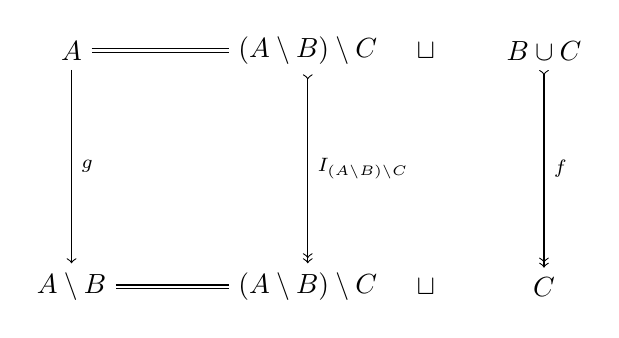
\begin{tikzpicture}[auto] 
    \node (a) at (0, 3) {$A$};
    \node (b) at (3, 3) {$\left( A\setminus B\right) \setminus C$};
    \node (c) at (4.5, 3) {$\sqcup $};
    \node (d) at (6, 3) {$B\cup C$};
    \node (e) at (0, 0) {$A\setminus B$};
    \node (f) at (3, 0) {$\left( A\setminus B\right) \setminus C$};
    \node (g) at (4.5, 0) {$\sqcup $};
    \node (h) at (6, 0) {$C$};
    \draw [->] (a) to node {$\scriptstyle g$} (e);
    \draw [>->>] (b) to node {$\scriptstyle I_{\left( A\setminus B\right) \setminus C}$} (f);
    \draw [>->>] (d) to node {$\scriptstyle f$} (h);
    \draw [double distance=1pt] (a) to node {$\scriptstyle $} (b);
    \draw [double distance=1pt] (e) to node {$\scriptstyle $} (f);
  \end{tikzpicture} 
\end{center}
その終集合$A \setminus B$について、次式が成り立つ、
\begin{center}
  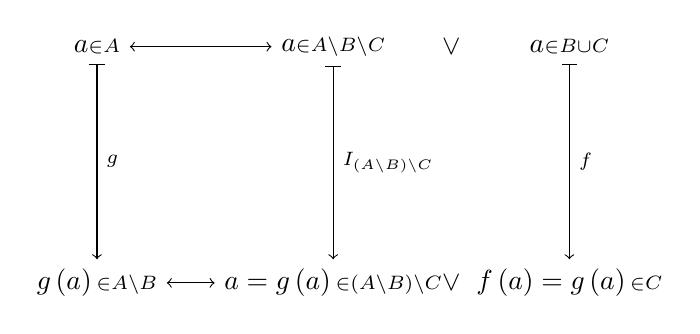
\begin{tikzpicture}[auto] 
    \node (i) at (0, 3) {$a{\scriptstyle\in A} $};
    \node (j) at (3, 3) {$a{\scriptstyle\in A\setminus B\setminus C}$};
    \node (k) at (4.5, 3) {$\vee $};
    \node (l) at (6, 3) {$a{\scriptstyle\in B\cup C}$};
    \node (m) at (0, 0) {$g\left( a\right) {\scriptstyle\in A\setminus B}$};
    \node (n) at (3, 0) {$a=g\left( a\right) {\scriptstyle\in \left( A\setminus B\right) \setminus C}$};
    \node (o) at (4.5, 0) {$\vee $};
    \node (p) at (6, 0) {$f\left( a\right) =g\left( a\right) {\scriptstyle\in C}$};
    \draw [|->] (i) to node {$\scriptstyle g$} (m);
    \draw [|->] (j) to node {$\scriptstyle I_{\left( A\setminus B\right) \setminus C}$} (n);
    \draw [|->] (l) to node {$\scriptstyle f$} (p);
    \draw [<->] (i) to node {$\scriptstyle $} (j);
    \draw [<->] (m) to node {$\scriptstyle $} (n);  
  \end{tikzpicture} 
\end{center}
即ち、$\forall g(a) \in A \setminus B$に対し、$g(a) \in (A \setminus B) \setminus C$または$g(a) \in B \cup C$が成り立つので、$\exists a \in A$に対し、次式が成り立つ。
\begin{align*}
g(a) = \left\{ \begin{matrix}
a & {\mathrm {if}} & a \in (A \setminus B) \setminus C \\
f(a) & {\mathrm {if}} & a \in B \cup C \\
\end{matrix} \right.\ 
\end{align*}
ここで、写像$I_{A}':A \rightarrow A \setminus B;a \mapsto a$が単射であるので、写像$I_{A}'':A \rightarrow (A \setminus B) \setminus C;a \mapsto a$が全単射であるかつ、その写像$f$は全単射であったので、その写像$g$も全単射となる。よって、その集合$A \setminus B$はその集合$A$と対等である。ある無限集合$A$とあるたかだか可算な集合$B$について集合$A \cup B$が無限集合であるなら、集合$(A \cup B) \setminus A$は、次式が成り立つので、
\begin{align*}
(A \cup B) \setminus A = A \setminus A \cup B \setminus A = \emptyset \cup B \setminus A = B \setminus A
\end{align*}
その集合$B$に含まれたかだか可算な集合となる。したがって、ある無限集合$A$と$B \in \mathfrak{P}(A)$なるたかだか可算な集合$B$について$A \setminus B$が無限集合であるなら、その集合$A \setminus B$はその集合$A$と対等であったので、その集合$(A \cup B) \setminus \left( (A \cup B) \setminus A \right)$はその集合$A \cup B$と対等である。また、その集合$(A \cup B) \setminus \left( (A \cup B) \setminus A \right)$を$U$とおくと、次のようになるので、
\begin{align*}
U &= (A \cup B) \setminus \left( (A \cup B) \setminus A \right)\\
&= (A \cup B) \setminus (A \setminus A \cup B \setminus A)\\
&= (A \cup B) \setminus (\emptyset \cup B \setminus A)\\
&= (A \cup B) \setminus \emptyset \cap (A \cup B) \setminus (B \setminus A)\\
&= (A \cup B) \cap (A \cup B) \setminus (B \setminus A)\\
&= (A \cup B) \cap (A \cup B) \cap (A \cup U \setminus B)\\
&= (A \cup B) \cap (A \cup U \setminus B)\\
&= A \cup (B \cap A \setminus B) \\
&= A \cup \emptyset = A
\end{align*}
以上より、よって、その集合$A$はその集合$A \cup B$と対等である。
\end{proof}
%\hypertarget{ux51aaux96c6ux5408ux306eux6fc3ux5ea6}{%
\subsubsection{冪集合の濃度}%\label{ux51aaux96c6ux5408ux306eux6fc3ux5ea6}}
\begin{thm}\label{1.2.7.11}
任意の集合$A$とこれの冪集合$\mathfrak{P}(A)$について、その集合$A$の濃度$\# A$はその集合$\mathfrak{P}(A)の濃度\# {\mathfrak{P}(A)}$より小さい、即ち、$\# A < \# {\mathfrak{P}(A)}$が成り立つ。
\end{thm}\par
これにより、任意の濃度に対してもこれより大きいような濃度が必ず存在できるので、濃度はいくらでも大きいものが存在することができる。
\begin{proof}
任意の集合$A$とこれの冪集合$\mathfrak{P}(A)$について、次式のような写像$f$は明らかに単射である。
\begin{align*}
f:A \rightarrow \mathfrak{P}(A);a \mapsto \left\{ a \right\}
\end{align*}
これにより、$\# A \leq \# {\mathfrak{P}(A)}$が成り立つ。ここで、$\forall g \in \mathfrak{F}\left( A,\mathfrak{P}(A) \right)$に対し、次式のように集合$A'$が与えられたとする。
\begin{align*}
A' = \left\{ a \in A \middle| a \notin g(a) \right\}
\end{align*}
このとき、$\forall a \in A$に対し、その元$a$のその写像$g$による像$g(a)$はその集合$\mathfrak{P}(A)$の元となるので、$a \in A$が成り立つならそのときに限り、$a \in g(a)$または$a \in A \setminus g(a)$が成り立つ。ここで、$a \in g(a)$が成り立つなら、$a \notin A'$が成り立つので、$g(a) \neq A'$が成り立つ。一方で、$a \notin g(a)$が成り立つなら、その集合$A'$の定義より明らかに$a \in A'$が成り立つので、$g(a) \neq A'$が成り立つ。以上より、$\forall a \in A$に対し、$g(a) \neq A'$が成り立つので、次式のようになる。
\begin{align*}
\forall a \in A\left[ A' \notin V\left( g|\left\{ a \right\} \right) \right] &\Leftrightarrow \neg\exists a \in A\left[ A' \in V\left( g \middle| \left\{ a \right\} \right) \right]\\
&\Leftrightarrow \neg A' \in \bigcup_{a \in A} {V\left( g|\left\{ a \right\} \right)}\\
&\Leftrightarrow A' \notin V(g)
\end{align*}
これにより、$V(g)\subset \mathfrak{P}(A)$が成り立つので、その写像$g$は全射であることができない。したがって、$\# A < \# {\mathfrak{P}(A)}$が成り立つ。
\end{proof}
\begin{thebibliography}{50}
  \bibitem{1}
    松坂和夫, 集合・位相入門, 岩波書店, 1968. 新装版第2刷 p61-78 ISBM978-4-00-029871-1
\end{thebibliography}
\end{document}


\clearpage
\documentclass[dvipdfmx]{jsarticle}
\setcounter{section}{2}
\setcounter{subsection}{9}
\usepackage{xr}
\externaldocument{1.2.4}
\usepackage{amsmath,amsfonts,amssymb,array,comment,mathtools,url,docmute}
\usepackage{longtable,booktabs,dcolumn,tabularx,mathtools,multirow,colortbl,xcolor}
\usepackage[dvipdfmx]{graphics}
\usepackage{bmpsize}
\usepackage{amsthm}
\usepackage{enumitem}
\setlistdepth{20}
\renewlist{itemize}{itemize}{20}
\setlist[itemize]{label=•}
\renewlist{enumerate}{enumerate}{20}
\setlist[enumerate]{label=\arabic*.}
\setcounter{MaxMatrixCols}{20}
\setcounter{tocdepth}{3}
\newcommand{\rotin}{\text{\rotatebox[origin=c]{90}{$\in $}}}
\newcommand{\amap}[6]{\text{\raisebox{-0.7cm}{\begin{tikzpicture} 
  \node (a) at (0, 1) {$\textstyle{#2}$};
  \node (b) at (#6, 1) {$\textstyle{#3}$};
  \node (c) at (0, 0) {$\textstyle{#4}$};
  \node (d) at (#6, 0) {$\textstyle{#5}$};
  \node (x) at (0, 0.5) {$\rotin $};
  \node (x) at (#6, 0.5) {$\rotin $};
  \draw[->] (a) to node[xshift=0pt, yshift=7pt] {$\textstyle{\scriptstyle{#1}}$} (b);
  \draw[|->] (c) to node[xshift=0pt, yshift=7pt] {$\textstyle{\scriptstyle{#1}}$} (d);
\end{tikzpicture}}}}
\newcommand{\twomaps}[9]{\text{\raisebox{-0.7cm}{\begin{tikzpicture} 
  \node (a) at (0, 1) {$\textstyle{#3}$};
  \node (b) at (#9, 1) {$\textstyle{#4}$};
  \node (c) at (#9+#9, 1) {$\textstyle{#5}$};
  \node (d) at (0, 0) {$\textstyle{#6}$};
  \node (e) at (#9, 0) {$\textstyle{#7}$};
  \node (f) at (#9+#9, 0) {$\textstyle{#8}$};
  \node (x) at (0, 0.5) {$\rotin $};
  \node (x) at (#9, 0.5) {$\rotin $};
  \node (x) at (#9+#9, 0.5) {$\rotin $};
  \draw[->] (a) to node[xshift=0pt, yshift=7pt] {$\textstyle{\scriptstyle{#1}}$} (b);
  \draw[|->] (d) to node[xshift=0pt, yshift=7pt] {$\textstyle{\scriptstyle{#2}}$} (e);
  \draw[->] (b) to node[xshift=0pt, yshift=7pt] {$\textstyle{\scriptstyle{#1}}$} (c);
  \draw[|->] (e) to node[xshift=0pt, yshift=7pt] {$\textstyle{\scriptstyle{#2}}$} (f);
\end{tikzpicture}}}}
\renewcommand{\thesection}{第\arabic{section}部}
\renewcommand{\thesubsection}{\arabic{section}.\arabic{subsection}}
\renewcommand{\thesubsubsection}{\arabic{section}.\arabic{subsection}.\arabic{subsubsection}}
\everymath{\displaystyle}
\allowdisplaybreaks[4]
\usepackage{vtable}
\theoremstyle{definition}
\newtheorem{thm}{定理}[subsection]
\newtheorem*{thm*}{定理}
\newtheorem{dfn}{定義}[subsection]
\newtheorem*{dfn*}{定義}
\newtheorem{axs}[dfn]{公理}
\newtheorem*{axs*}{公理}
\renewcommand{\headfont}{\bfseries}
\makeatletter
  \renewcommand{\section}{%
    \@startsection{section}{1}{\z@}%
    {\Cvs}{\Cvs}%
    {\normalfont\huge\headfont\raggedright}}
\makeatother
\makeatletter
  \renewcommand{\subsection}{%
    \@startsection{subsection}{2}{\z@}%
    {0.5\Cvs}{0.5\Cvs}%
    {\normalfont\LARGE\headfont\raggedright}}
\makeatother
\makeatletter
  \renewcommand{\subsubsection}{%
    \@startsection{subsubsection}{3}{\z@}%
    {0.4\Cvs}{0.4\Cvs}%
    {\normalfont\Large\headfont\raggedright}}
\makeatother
\makeatletter
\renewenvironment{proof}[1][\proofname]{\par
  \pushQED{\qed}%
  \normalfont \topsep6\p@\@plus6\p@\relax
  \trivlist
  \item\relax
  {
  #1\@addpunct{.}}\hspace\labelsep\ignorespaces
}{%
  \popQED\endtrivlist\@endpefalse
}
\makeatother
\renewcommand{\proofname}{\textbf{証明}}
\usepackage{tikz,graphics}
\usepackage[dvipdfmx]{hyperref}
\usepackage{pxjahyper}
\hypersetup{
 setpagesize=false,
 bookmarks=true,
 bookmarksdepth=tocdepth,
 bookmarksnumbered=true,
 colorlinks=false,
 pdftitle={},
 pdfsubject={},
 pdfauthor={},
 pdfkeywords={}}
\begin{document}
%\hypertarget{ux6fc3ux5ea6ux306eux6f14ux7b97}{%
\subsection{濃度の演算}%\label{ux6fc3ux5ea6ux306eux6f14ux7b97}}
%\hypertarget{ux6fc3ux5ea6ux306eux6f14ux7b97-1}{%
\subsubsection{濃度の演算}%\label{ux6fc3ux5ea6ux306eux6f14ux7b97-1}}
\begin{dfn}
任意の$A \cap B = \emptyset $なる2つの集合たち$A$、$B$について、次式のように定義する。
\begin{align*}
\# A + \# B = \# (A \sqcup B)
\end{align*}
\end{dfn}
\begin{thm}\label{1.2.8.1}
この定義は集合によらない、即ち、$\# A = \# A'$かつ$\# B = \# B'$となるような集合たち$A'$、$B'$が存在するなら、$\# A + \# B = \# A' + \# B'$が成り立つ。
\end{thm}
\begin{proof}
任意の$A \cap B = \emptyset $なる2つの集合たち$A$、$B$について、次式のように定義する。
\begin{align*}
\# A + \# B = \# (A \sqcup B)
\end{align*}
さらに、$A \sim A'$かつ$B \sim B'$かつ$A' \cap B' = \emptyset $なる集合たち$A'$、$B'$を考えると、全単射たち$f_{A}$、$f_{B}$がそれぞれ集合$\mathfrak{F}\left( A,A' \right)$、$\mathfrak{F}\left( B,B' \right)$に存在するのであったので、次式のように写像$g$が定義されると、
\begin{align*}
g:A \sqcup B \rightarrow A' \sqcup B';a \mapsto \left\{ \begin{matrix}
f_{A}(a) & {\mathrm{if}} & a \in A \\
f_{B}(a) & {\mathrm{if}} & a \in B \\
\end{matrix} \right.\ 
\end{align*}
それらの写像たち$f_{A}$、$f_{B}$が全単射であったので、$V\left( f_{A} \right) = A'$かつ$V\left( f_{B} \right) = B'$が成り立つかつ、逆写像たち$f_{A}^{- 1}$、$f_{B}^{- 1}$が存在するかつ、$A' \cap B' = \emptyset $が成り立つことに注意すれば、次式のように逆写像$g^{- 1}$が存在するので、
\begin{align*}
g^{- 1}:A' \sqcup B' \rightarrow A \sqcup B;b \mapsto \left\{ \begin{matrix}
f_{A}^{- 1}(b) & {\mathrm{if}} & b \in A' \\
f_{B}^{- 1}(b) & {\mathrm{if}} & b \in B' \\
\end{matrix} \right.\ 
\end{align*}
その写像$g$は全単射となる。したがって、$A \sqcup B \sim A' \sqcup B'$が成り立つので、次式が成り立つ。
\begin{align*}
\# (A \sqcup B) = \# \left( A' \sqcup B' \right)
\end{align*}
\end{proof}
\begin{thm}\label{1.2.8.2}
任意の濃度たち$\mathfrak{m}$、$\mathfrak{n}$に対し、次式のような集合たち$A$、$B$が存在する。
\begin{align*}
\mathfrak{m} =\# A,\ \ \mathfrak{n} =\# B,\ \ A \cap B = \emptyset 
\end{align*}
\end{thm}
\begin{proof}
任意の濃度たち$\mathfrak{m}$、$\mathfrak{n}$に対し、定義より明らかに次式のような集合たち$A$、$B$が存在する。
\begin{align*}
\mathfrak{m} =\# A,\ \ \mathfrak{n} =\# B
\end{align*}
ここで、$A \cap B = \emptyset $が成り立つなら、示すべきことは示されている。\par
$A \cap B \neq \emptyset $が成り立つなら、次式のような写像たち$f_{A}$、$f_{B}$が考えられれば、
\begin{align*}
f_{A}&:A \rightarrow A \times \left\{ 0 \right\};a \mapsto (a,0)\\
f_{B}&:B \rightarrow B \times \left\{ 1 \right\};b \mapsto (b,1)
\end{align*}
これらの写像たち$f_{A}$、$f_{B}$は明らかに全単射となるので、$A \sim A \times \left\{ 0 \right\}$かつ$B \sim B \times \left\{ 1 \right\}$が成り立つかつ、$0 \neq 1$より$\left( A \times \left\{ 0 \right\} \right) \cap \left( B \times \left\{ 1 \right\} \right) = \emptyset $が成り立つことになるので、次式が成り立ち、
\begin{align*}
\# \left( A \times \left\{ 0 \right\} \right) = \# A = \mathfrak{m},\ \ \# \left( B \times \left\{ 1 \right\} \right) = \# B = \mathfrak{n,\ \ }\left( A \times \left\{ 0 \right\} \right) \cap \left( B \times \left\{ 1 \right\} \right) = \emptyset 
\end{align*}
よって、示すべきことは示された。
\end{proof}
\begin{thm}\label{1.2.8.3}
次のことが成り立つ\footnote{これにより濃度は可換群のように計算されることができる。}。
\begin{itemize}
\item
  $\forall\# A,\# B,\# C \in \mathcal{F} /\sim $に対し、次式が成り立つ。
\begin{align*}
\left( \# A + \# B \right) + \# C = \# A + \left( \# B + \# C \right)
\end{align*}
\item
  $\forall\# A \in \mathcal{F} /\sim $に対し、次式が成り立つ。
\begin{align*}
\# A + \# \emptyset  = \# A
\end{align*}
\item
  $\forall\# A,\# B \in \mathcal{F} /\sim $に対し、次式が成り立つ。
\begin{align*}
\# A + \# B = \# B + \# A
\end{align*}
\item
  $\forall\# A,\# B,\# C,\# D \in \mathcal{F} /\sim $に対し、$\# A \leq \# B$かつ$\# C \leq \# D$が成り立つなら、次式が成り立つ。
\begin{align*}
\# A + \# C \leq \# B + \# D
\end{align*}
\end{itemize}
\end{thm}
\begin{proof}
$\forall\# A,\# B,\# C \in \mathcal{F} /\sim $に対し、次のようになる。
\begin{align*}
\left( \# A + \# B \right) + \# C &= \# (A \sqcup B) + \# C\\
&= \# \left( (A \sqcup B) \sqcup C \right)\\
&= \# \left( A \sqcup (B \sqcup C) \right)\\
&= \# A + \# (B \sqcup C)\\
&= \# A + \left( \# B + \# C \right)
\end{align*}\par
$\forall\# A \in \mathcal{F} /\sim $に対し、次のようになる。
\begin{align*}
\# A + \# \emptyset  = \# (A \sqcup \emptyset ) = \# A
\end{align*}\par
$\forall\# A,\# B \in \mathcal{F} /\sim $に対し、次のようになる。
\begin{align*}
\# A + \# B &= \# (A \sqcup B)\\
&= \# (B \sqcup A)\\
&= \# B + \# A
\end{align*}\par
$\forall\# A,\# B,\# C,\# D \in \mathcal{F} /\sim $に対し、$\# A \leq \# B$かつ$\# C \leq \# D$が成り立つなら、次式のように単射な写像たち$f_{A}$、$f_{B}$が存在する。
\begin{align*}
f_{A}:A \rightarrowtail B,\ \ f_{B}:C \rightarrowtail D
\end{align*}
ここで、次のような写像たち$f_{A}'$、$f_{B}'$、$f_{A}''$、$f_{B}''$が定義されると、
\begin{align*}
f_{A}':A \rightarrow A \times \left\{ 0 \right\};a \mapsto (a,0),\ \ f_{B}':C \rightarrow C \times \left\{ 1 \right\};b \mapsto (b,1),\\
f_{A}'':B \rightarrow B \times \left\{ 0 \right\};a \mapsto (a,0),\ \ f_{B}'':D \rightarrow D \times \left\{ 1 \right\};b \mapsto (b,1)
\end{align*}
明らかにこれらの写像たち$f_{A}'$、$f_{B}'$、$f_{A}''$、$f_{B}''$は全単射となるので、次式たちが成り立つ。
\begin{align*}
\# A = \# \left( A \times \left\{ 0 \right\} \right),\ \ \# C = \# \left( C \times \left\{ 1 \right\} \right),\\
\# B = \# \left( B \times \left\{ 0 \right\} \right),\ \ \# D = \# \left( D \times \left\{ 1 \right\} \right)
\end{align*}
さらに、$\left( A \times \left\{ 0 \right\} \right) \cap \left( C \times \left\{ 1 \right\} \right) = \left( B \times \left\{ 0 \right\} \right) \cap \left( D \times \left\{ 1 \right\} \right) = \emptyset $が成り立つので、次式たちが成り立つ。
\begin{align*}
\# A + \# C &= \# \left( A \times \left\{ 0 \right\} \right) + \# \left( C \times \left\{ 1 \right\} \right)\\
&= \# \left( \left( A \times \left\{ 0 \right\} \right) \sqcup \left( C \times \left\{ 1 \right\} \right) \right)\\
\# B + \# D &= \# \left( B \times \left\{ 0 \right\} \right) + \# \left( D \times \left\{ 1 \right\} \right)\\
&= \# \left( \left( B \times \left\{ 0 \right\} \right) \sqcup \left( D \times \left\{ 1 \right\} \right) \right)
\end{align*}
ここで、次式のように写像$g$が定義されると、
\begin{align*}
g:\left( A \times \left\{ 0 \right\} \right) \sqcup \left( C \times \left\{ 1 \right\} \right) \rightarrow \left( B \times \left\{ 0 \right\} \right) \sqcup \left( D \times \left\{ 1 \right\} \right);(a,b) \mapsto \left\{ \begin{matrix}
\left( f_{A}(a),0 \right) & {\mathrm{if}} & (a,b) \in A \times \left\{ 0 \right\} \\
\left( f_{B}(a),1 \right) & {\mathrm{if}} & (a,b) \in C \times \left\{ 1 \right\} \\
\end{matrix} \right.\ 
\end{align*}
これらの写像たち$f_{A}$、$f_{B}$は単射であったので、明らかにこの写像$g$も単射となる。\par
したがって、次式が成り立つ。
\begin{align*}
\# \left( \left( A \times \left\{ 0 \right\} \right) \sqcup \left( C \times \left\{ 1 \right\} \right) \right) \leq \# \left( \left( B \times \left\{ 0 \right\} \right) \sqcup \left( D \times \left\{ 1 \right\} \right) \right)
\end{align*}
よって、次式が成り立つ。
\begin{align*}
\# A + \# C \leq \# B + \# D
\end{align*}
\end{proof}
\begin{dfn}
任意の2つの集合たち$A$、$B$について、次式のように定義する。
\begin{align*}
\# A \cdot \# B = \# (A \times B)
\end{align*}
\end{dfn}
\begin{thm}\label{1.2.8.4}
この定義は集合によらない、即ち、$\# A = \# A'$かつ$\# B = \# B'$となるような集合たち$A'$、$B'$が存在するなら、$\# A \cdot \# B = \# A' \cdot \# B'$が成り立つ。
\end{thm}
\begin{proof} 任意の2つの集合たち$A$、$B$について、次式のように定義する。
\begin{align*}
\# A \cdot \# B = \# (A \times B)
\end{align*}
さらに、$A \sim A'$かつ$B \sim B'$かつ$A' \cap B' = \emptyset $なる集合たち$A'$、$B'$を考えると、全単射たち$f_{A}$、$f_{B}$がそれぞれ集合$\mathfrak{F}\left( A,A' \right)$、$\mathfrak{F}\left( B,B' \right)$に存在するのであったので、次式のように写像$g$が定義されると、
\begin{align*}
g:A \times B \rightarrow A' \times B';(a,b) \mapsto \left( f_{A}(a),f_{B}(b) \right)
\end{align*}
次式のようにこれの逆写像$g^{- 1}$が存在するので、
\begin{align*}
g^{- 1}:A' \times B' \rightarrow A \times B;\left( a',b' \right) \mapsto \left( f_{A}^{- 1}\left( a' \right),f_{B}^{- 1}\left( b' \right) \right)
\end{align*}
その写像$g$は全単射となる。したがって、$A \times B \sim A' \times B'$が成り立ち、したがって、次のようになる。
\begin{align*}
\# A \cdot \# B &= \# (A \times B)\\
&= \# \left( A' \times B' \right)\\
&= \# A' \cdot \# B'
\end{align*}
\end{proof}
\begin{thm}\label{1.2.8.5}
次のことが成り立つ。
\begin{itemize}
\item
  $\forall\# A,\# B,\# C \in \mathcal{F} /\sim $に対し、次式が成り立つ。
\begin{align*}
\left( \# A \cdot \# B \right) \cdot \# C = \# A \cdot \left( \# B \cdot \# C \right)
\end{align*}
\item
  $\forall\# A \in \mathcal{F} /\sim $に対し、次式が成り立つ。
\begin{align*}
\# A \cdot \# \emptyset  = \# \emptyset 
\end{align*}
\item
  $\forall\# A \in \mathcal{F} /\sim $に対し、次式が成り立つ。
\begin{align*}
\# A \cdot \# \left\{ 1 \right\} = \# A
\end{align*}
\item
  $\forall\# A,\# B \in \mathcal{F} /\sim $に対し、次式が成り立つ。
\begin{align*}
\# A \cdot \# B = \# B \cdot \# A
\end{align*}
\item
  $\forall\# A,\# B,\# C,\# D \in \mathcal{F} /\sim $に対し、$\# A \leq \# B$かつ$\# C \leq \# D$が成り立つなら、次式が成り立つ。
\begin{align*}
\# A \cdot \# C \leq \# B \cdot \# D
\end{align*}
\item
  $\forall\# A,\# B,\# C \in \mathcal{F} /\sim $に対し、次式が成り立つ。
\begin{align*}
\# A \cdot \left( \# B + \# C \right) = \left( \# A \cdot \# B \right) + \left( \# A \cdot \# C \right)
\end{align*}
\end{itemize}
\end{thm}
\begin{proof}
$\forall\# A,\# B,\# C \in \mathcal{F} /\sim $に対し、次のようになる。
\begin{align*}
\left( \# A \cdot \# B \right) \cdot \# C &= \# (A \times B) \cdot \# C\\
&= \# \left( (A \times B) \times C \right)
\end{align*}
ここで、次式のような写像$f$が考えられれば、
\begin{align*}
f:(A \times B) \times C \rightarrow A \times (B \times C);\left( (a,b),c \right) \mapsto \left( a,(b,c) \right)
\end{align*}
これは明らかに全単射となるので、次のようになる。
\begin{align*}
\left( \# A \cdot \# B \right) \cdot \# C &= \# \left( (A \times B) \times C \right)\\
&= \# \left( A \times (B \times C) \right)\\
&= \# A \cdot \# (B \times C)\\
&= \# A \cdot \left( \# B \cdot \# C \right)
\end{align*}\par
$\forall\# A \in \mathcal{F} /\sim $に対し、次のようになる。
\begin{align*}
\# A \cdot \# \emptyset  = \# (A \times \emptyset ) = \# \emptyset 
\end{align*}\par
$\forall\# A \in \mathcal{F} /\sim $に対し、次式のような写像$f$が考えられれば、
\begin{align*}
f:A \rightarrow A \times \left\{ 1 \right\};a \mapsto (a,1)
\end{align*}
これは明らかに全単射となるので、次のようになる。
\begin{align*}
\# A \cdot \# \left\{ 1 \right\} = \# \left( A \times \left\{ 1 \right\} \right) = \# A
\end{align*}\par
$\forall\# A,\# B \in \mathcal{F} /\sim $に対し、次式のような写像$f$が考えられれば、
\begin{align*}
f:A \times B \rightarrow B \times A;(a,b) \mapsto (b,a)
\end{align*}
これは明らかに全単射となるので、次のようになる。
\begin{align*}
\# A \cdot \# B &= \# (A \times B)\\
&= \# (B \times A)\\
&= \# B \cdot \# A
\end{align*}\par
$\forall\# A,\# B,\# C,\# D \in \mathcal{F} /\sim $に対し、$\# A \leq \# B$かつ$\# C \leq \# D$が成り立つなら、次式のように単射な写像たち$f_{A}$、$f_{B}$が存在する。
\begin{align*}
f_{A}:A \rightarrowtail B,\ \ f_{B}:C \rightarrowtail D
\end{align*}
ここで、次式のように写像$g$が定義されると、
\begin{align*}
g:A \times C \rightarrow B \times D;(a,b) \mapsto \left( f_{A}(a),f_{B}(b) \right)
\end{align*}
これらの写像たち$f_{A}$、$f_{B}$は単射であったので、明らかにこの写像$g$も単射となる。したがって、次式が成り立つ。
\begin{align*}
\# (A \times C) \leq \# (B \times D)
\end{align*}
よって、次式が成り立つ。
\begin{align*}
\# A \cdot \# C \leq \# B \cdot \# D
\end{align*}\par
$\forall\# A,\# B,\# C \in \mathcal{F} /\sim $に対し、$A \times (B \sqcup C) = (A \times B) \sqcup (A \times C)$が成り立つことに注意すれば、次のようになる。
\begin{align*}
\# A \cdot \left( \# B + \# C \right) &= \# A \cdot \# (B \sqcup C)\\
&= \# \left( A \times (B \sqcup C) \right)\\
&= \# \left( (A \times B) \sqcup (A \times C) \right)\\
&= \# (A \times B) + \# (A \times C)\\
&= \# A \cdot \# B + \# A \cdot \# C
\end{align*}
\end{proof}
\begin{thm}\label{1.2.8.6}
添数集合$\varLambda$によって添数づけられた集合族$\left( A_{\lambda} \right)_{\lambda \in \varLambda}$が与えられ、$\forall\lambda \in \varLambda$に対し、$\# A_{\lambda} = \mathfrak{n}$が成り立つとき、次式が成り立つ。
\begin{align*}
\# {\bigsqcup_{\lambda \in \varLambda} A_{\lambda}} = \# \varLambda\mathfrak{\cdot n}
\end{align*}
\end{thm}
\begin{proof}
添数集合$\varLambda$によって添数づけられた集合族$\left( A_{\lambda} \right)_{\lambda \in \varLambda}$が与えられ、$\forall\lambda \in \varLambda$に対し、$\# A_{\lambda} = \mathfrak{n}$が成り立つとき、$\lambda' \in \varLambda$なる1つの添数$\lambda'$を用いると、$\forall\lambda \in \varLambda$に対し、次式のような全単射な写像$f_{\lambda}$が存在する。
\begin{align*}
f_{\lambda}:A_{\lambda'}\overset{\sim}{\rightarrow}A_{\lambda}
\end{align*}
ここで、次式のような写像$f$が考えられる。
\begin{align*}
f:A_{\lambda'} \times \varLambda \rightarrow \bigsqcup_{\lambda \in \varLambda} A_{\lambda};(a,\lambda) \mapsto f_{\lambda}(a)
\end{align*}
$\forall b \in \bigsqcup_{\lambda \in \varLambda} A_{\lambda}$に対し、$\exists\lambda \in \varLambda\left[ b \in A_{\lambda} \right]$が成り立つので、$b \in A_{\lambda}$なる添数$\lambda$が存在する。さらに、その写像$f_{\lambda}$は全射であったので、$f_{\lambda}(a) = b$なる元$a$がその集合$A_{\lambda'}$に存在する。したがって、$f(a,\lambda) = f_{\lambda}(a) = b$なる順序づけられた組$(a,\lambda)$がその集合$A_{\lambda'} \times \varLambda$に存在することになるので、その写像$f$は全射となることが示された。\par
$\forall(a,\lambda),(b,\mu) \in A_{\lambda'} \times \varLambda$に対し、$(a,\lambda) \neq (b,\mu)$が成り立つなら、$a \neq b$または$\lambda \neq \mu$が成り立つ。ここで、$\lambda \neq \mu$が成り立つとき、$A_{\lambda} \cap A_{\mu} = \emptyset $が成り立つかつ、$f_{\lambda}(a) \in A_{\lambda}$かつ$f_{\mu}(b) \in A_{\mu}$が成り立つので、$f_{\lambda}(a) = f_{\mu}(b)$が成り立たない。したがって、$f(a,\lambda) \neq f(b,\mu)$が成り立つ。一方で、$\lambda = \mu$かつ$a \neq b$のとき、それらの写像たち$f_{\lambda}$、$f_{\mu}$は単射であったので、$f_{\lambda}(a) \neq f_{\mu}(b)$が成り立ち、したがって、$f(a,\lambda) \neq f(b,\mu)$が成り立つ。以上より、その写像$f$は単射であることが示された。\par
したがって、その写像$f$は全単射となるので、次式が成り立つ。
\begin{align*}
\# \left( A_{\lambda'} \times \varLambda \right) = \# {\bigsqcup_{\lambda \in \varLambda} A_{\lambda}}
\end{align*}
これにより、次のようになる。
\begin{align*}
\# {\bigsqcup_{\lambda \in \varLambda} A_{\lambda}} &= \# \left( A_{\lambda'} \times \varLambda \right)\\
&= \# A_{\lambda'} \cdot \# \varLambda\\
&= \# \varLambda \cdot \# A_{\lambda'}\\
&= \# \varLambda\mathfrak{\cdot n}
\end{align*}
\end{proof}
\begin{dfn}
任意の2つの集合たち$A$、$B$について、次式のように定義する。
\begin{align*}
{\# B}^{\# A} = \# {\mathfrak{F}(A,B)}
\end{align*}
\end{dfn}
\begin{thm}\label{1.2.8.7}
このとき、この定義は集合によらない、即ち、$\# A = \# A'$かつ$\# B = \# B'$となるような集合たち$A'$、$B'$が存在するなら、${\# B}^{\# A} = {\# B'}^{\# A'}$が成り立つ。
\end{thm}
\begin{proof} 任意の2つの集合たち$A$、$B$について、次式のように定義する。
\begin{align*}
{\# B}^{\# A} = \# {\mathfrak{F}(A,B)}
\end{align*}
さらに、$A \sim A'$かつ$B \sim B'$かつ$A' \cap B' = \emptyset $なる集合たち$A'$、$B'$を考えると、全単射たち$f_{A}$、$f_{B}$がそれぞれ集合$\mathfrak{F}\left( A,A' \right)$、$\mathfrak{F}\left( B,B' \right)$に存在するのであったので、次式のように写像$g$が定義されると、
\begin{align*}
g:\mathfrak{F}(A,B)\mathfrak{\rightarrow F}\left( A',B' \right);f \mapsto f_{B} \circ f \circ f_{A}^{- 1}
\end{align*}
即ち、次式のように写像$g$が定義されると、
\begin{center}
  \begin{tikzpicture}[auto] 
    \node (a) at (0, 0) {$A'$};
    \node (b) at (0, 3) {$A$};
    \node (c) at (3, 0) {$B'$};
    \node (d) at (3, 3) {$B$};
    \draw [->] (b) to node {$\scriptstyle f$} (d);
    \draw [>->>] (b) to node {$\scriptstyle f_A $} (a);
    \draw [>->>] (d) to node {$\scriptstyle f_B $} (c);
    \draw [->] (a) to node {$\scriptstyle f_B \circ f\circ f_{A}^{-1} $} (c);
    \end{tikzpicture} 
\end{center}
次式のように逆写像$g^{- 1}$が存在するので、
\begin{align*}
g^{- 1}\mathfrak{:F}\left( A',B' \right)\mathfrak{\rightarrow F}(A,B);f \mapsto f_{B}^{- 1} \circ f \circ f_{A}
\end{align*}
その写像$g$は全単射となる。\par
したがって、$\mathfrak{F}(A,B)\mathfrak{\sim F}\left( A',B' \right)$が成り立ち、したがって、次のようになる。
\begin{align*}
{\# B}^{\# A} &= \# {\mathfrak{F}(A,B)}\\
&= \# {\mathfrak{F}\left( A',B' \right)}\\
&= {\# B'}^{\# A'}
\end{align*}
\end{proof}
\begin{thm}\label{1.2.8.8}
次のことが成り立つ\footnote{これはいわゆる指数法則である。}。
\begin{itemize}
\item
  $\forall\# A,\# B,\# C \in \mathcal{F} /\sim $に対し、$B \cap C = \emptyset $が成り立つとすると、次式が成り立つ。
\begin{align*}
{\# A}^{\# B} \cdot {\# A}^{\# C} = {\# A}^{\# B + \# C}
\end{align*}
\item
  $\forall\# A,\# B,\# C \in \mathcal{F} /\sim $に対し、次式が成り立つ。
\begin{align*}
\left( \# B \cdot \# C \right)^{\# A} = {\# B}^{\# A} \cdot {\# C}^{\# A}
\end{align*}
\item
  $\forall\# A,\# B,\# C \in \mathcal{F} /\sim $に対し、次式が成り立つ。
\begin{align*}
\left( {\# A}^{\# B} \right)^{\# C} = {\# A}^{\# B \cdot \# C}
\end{align*}
\end{itemize}
\end{thm}
\begin{proof}
$\forall\# A,\# B,\# C \in \mathcal{F} /\sim $に対し、$B \cap C = \emptyset $が成り立つとする。$\forall f \in \mathfrak{F}(B \sqcup C,A)$に対し、$f|B \in \mathfrak{F}(B,A)$かつ$f|C \in \mathfrak{F}(C,A)$が成り立つので、その集合$\mathfrak{F}(B,A)\mathfrak{\times F}(C,A)$の元$\left( f|B,f|C \right)$がただ1つ決まる。逆に、このような元$\left( f|B,f|C \right)$が1つ決まると、仮定より$B \cap C = \emptyset $が成り立つので、次式のような写像$f$がただ1つ決まる。
\begin{align*}
f:B \sqcup C \rightarrow A;a \mapsto \left\{ \begin{matrix}
f|B(a) & {\mathrm{if}} & a \in B \\
f|C(a) & {\mathrm{if}} & a \in C \\
\end{matrix} \right.\ 
\end{align*}
このようにして、定められる次式のような写像$\mathfrak{f}$は、
\begin{align*}
\mathfrak{f:F}(B \sqcup C,A)\mathfrak{\rightarrow F}(B,A)\mathfrak{\times F}(C,A);f \mapsto \left( f|B,f|C \right)
\end{align*}
逆写像が構成されているので、全単射でありしたがって、次式が成り立つ。
\begin{align*}
\# {\mathfrak{F}(B \sqcup C,A)} = \# \left( \mathfrak{F}(B,A)\mathfrak{\times F}(C,A) \right)
\end{align*}
ここで、次のようになることから、
\begin{align*}
\# \left( \mathfrak{F}(B,A)\mathfrak{\times F}(C,A) \right) &= \# {\mathfrak{F}(B,A)} \cdot \# {\mathfrak{F}(C,A)}\\
&= {\# A}^{\# B} \cdot {\# A}^{\# C}\\
\# {\mathfrak{F}(B \sqcup C,A)} &= {\# A}^{\# {B \sqcup C}}\\
&= {\# A}^{\# B + \# C}
\end{align*}
よって、次式が成り立つ。
\begin{align*}
{\# A}^{\# B} \cdot {\# A}^{\# C} = {\# A}^{\# B + \# C}
\end{align*}\par
$\forall\# A,\# B,\# C \in \mathcal{F} /\sim $に対し、集合$B \times C$からその集合$B$への射影、その集合$C$への射影をそれぞれ${\mathrm{pr}}_{1}$、${\mathrm{pr}}_{2}$とすると、$\forall f \in \mathfrak{F}(A,B \times C)$に対し、${\mathrm{pr}}_{1} \circ f \in \mathfrak{F}(A,B)$かつ${\mathrm{pr}}_{2} \circ f\in \mathfrak{F}(A,C)$が成り立つので、その集合$\mathfrak{F}(A,B)\mathfrak{\times F}(A,C)$の元$\left( {\mathrm{pr}}_{1} \circ f,{\mathrm{pr}}_{2} \circ f \right)$がただ1つ決まる。逆に、このような元$\left( {\mathrm{pr}}_{1} \circ f,{\mathrm{pr}}_{2} \circ f \right)$が1つ決まると、次式のような写像$f$がただ1つ決まる。
\begin{align*}
f:A \rightarrow B \times C;a \mapsto \left( {\mathrm{pr}}_{1} \circ f(a),{\mathrm{pr}}_{2} \circ f(a) \right) = f(a)
\end{align*}
このようにして、定められる次式のような写像$\mathfrak{f}$は、
\begin{align*}
\mathfrak{f:F}(A,B \times C)\mathfrak{\rightarrow F}(A,B)\mathfrak{\times F}(A,C);f \mapsto \left( {\mathrm{pr}}_{1} \circ f,{\mathrm{pr}}_{2} \circ f \right)
\end{align*}
逆写像が構成されているので、全単射でありしたがって、次式が成り立つ。
\begin{align*}
\# {\mathfrak{F}(A,B \times C)} = \# \left( \mathfrak{F}(A,B)\mathfrak{\times F}(A,C) \right)
\end{align*}
ここで、次のようになることから、
\begin{align*}
\# {\mathfrak{F}(A,B \times C)} &= {\# {B \times C}}^{\# A}\\
&= \left( \# B \cdot \# C \right)^{\# A}\\
\# \left( \mathfrak{F}(A,B)\mathfrak{\times F}(A,C) \right) &= \# {\mathfrak{F}(A,B)} \cdot \# {\mathfrak{F}(A,C)}\\
&= {\# B}^{\# A} \cdot {\# C}^{\# A}
\left( \# B \cdot \# C \right)^{\# A} \\
&= {\# B}^{\# A} \cdot {\# C}^{\# A}
\end{align*}\par
$\forall\# A,\# B,\# C \in \mathcal{F} /\sim \forall f \in \mathfrak{F}(B \times C,A)$に対し、その集合$C$の1つの元$c$を用いて次式のような写像$f_{c}$を考えると、
\begin{align*}
\left( f_{c}:B \rightarrow A;b \mapsto f(b,c) \right)\in \mathfrak{F}(B,A)
\end{align*}
$\forall c \in C$に対し、この写像$f_{c}$がただ1つ決まる。ここで、次式のような写像$\widetilde{f}$が考えられれば、
\begin{align*}
\left( \widetilde{f}:C \mapsto \mathfrak{F}(B,A);c \mapsto f_{c} \right)\in \mathfrak{F}\left( C,\mathfrak{F}(B,A) \right)
\end{align*}
$\forall(b,c) \in B \times C$に対し、$f(b,c) = f_{c}(b) = \left( \widetilde{f}(c) \right)(b)$が成り立つので、その写像$\widetilde{f}$もただ1つ決まる。逆に、このような元$\widetilde{f}$が1つ決まるとき、次式のような写像$f'$が考えられれば、
\begin{align*}
f':B \times C \rightarrow A;(b,c) \mapsto \left( \widetilde{f}(c) \right)(b)
\end{align*}
$\widetilde{f} = \widetilde{f'}$が成り立つので、その写像$f'$はただ1つ決まる。このようにして、定められる次式のような写像$\mathfrak{f}$は、
\begin{align*}
\mathfrak{f:F}(B \times C,A)\mathfrak{\rightarrow F}\left( C,\mathfrak{F}(B,A) \right);f \mapsto \widetilde{f}
\end{align*}
逆写像が構成されているので、全単射でありしたがって、次式が成り立つ。
\begin{align*}
\# {\mathfrak{F}(B \times C,A)} = \# {\mathfrak{F}\left( C,\mathfrak{F}(B,A) \right)}
\end{align*}
ここで、次のようになることから、
\begin{align*}
\# {\mathfrak{F}\left( C,\mathfrak{F}(B,A) \right)} &= {\# {\mathfrak{F}(B,A)}}^{\# C}\\
&= \left( {\# A}^{\# B} \right)^{\# C}\\
\# {\mathfrak{F}(B \times C,A)} &= {\# A}^{\# {B \times C}}\\
&= {\# A}^{\# B \cdot \# C}
\end{align*}
よって、
\begin{align*}
\left( {\# A}^{\# B} \right)^{\# C} = {\# A}^{\# B \cdot \# C}
\end{align*}
\end{proof}
\begin{thm}\label{1.2.8.9}
任意の添数集合$\varLambda$によって添数づけられた集合の族$\left\{ A_{\lambda} \right\}_{\lambda \in \varLambda}$が与えられ、$\forall\lambda \in \varLambda$に対し、$A_{\lambda} = A$が成り立つとする。このとき、次式が成り立つ。
\begin{align*}
\# {\prod_{\lambda \in \varLambda} A_{\lambda}} = {\# A}^{\# \varLambda}
\end{align*}
\end{thm}
\begin{proof}
任意の添数集合$\varLambda$によって添数づけられた集合の族$\left\{ A_{\lambda} \right\}_{\lambda \in \varLambda}$が与えられ、$\forall\lambda \in \varLambda$に対し、$A_{\lambda} = A$が成り立つとする。このとき、直積の定義より次式が成り立つ。
\begin{align*}
\prod_{\lambda \in \varLambda} A_{\lambda} &= \left\{ f \in \mathfrak{F}\left( \varLambda,\bigcup_{\lambda \in \varLambda} A_{\lambda} \right) \middle| \forall\lambda \in \varLambda\left[ f(\lambda) \in A_{\lambda} \right] \right\}\\
&= \left\{ f \in \mathfrak{F}(\varLambda,A) \middle| \forall\lambda \in \varLambda\left[ f(\lambda) \in A \right] \right\} = \mathfrak{F}(\varLambda,A)
\end{align*}
これにより、次のようになる。
\begin{align*}
\# {\prod_{\lambda \in \varLambda} A_{\lambda}} = \# {\mathfrak{F}(\varLambda,A)} = {\# A}^{\# \varLambda}
\end{align*}
\end{proof}
\begin{thm}\label{1.2.8.10}
集合$A$の部分集合系$\mathfrak{P}(A)$について、次式が成り立つ\footnote{なお、無限集合$A$について、次のことが成り立つことが知られているが、この証明にZornの補題を用いる必要があるため、のちに述べることとする。
\begin{align*}
  \# B \leq \# A &\Rightarrow \# A + \# B = \# A\\
  1 \leq \# B \leq \# A &\Rightarrow \# A\# B = \# A\\
  2 \leq \# B \leq \# A &\Rightarrow 2^{\# A} = {\# B}^{\# A}
\end{align*}}。
\begin{align*}
\# {\mathfrak{P}(A)} = \# {\mathfrak{F}\left( A,\left\{ 0,1 \right\} \right)} = 2^{\# A}
\end{align*}
\end{thm}
\begin{proof}
集合$A$の部分集合系$\mathfrak{P}(A)$について、$\forall A'\in \mathfrak{P}(A)$に対し、その集合$A'$をこれの指示関数$\chi_{A'}$へうつす写像$\Phi$を考えると、その写像$\Phi$は全単射であったので、次式が成り立つ。
\begin{align*}
\# {\mathfrak{P}(A)} = \# {\mathfrak{F}\left( A,\left\{ 0,1 \right\} \right)} = 2^{\# A}
\end{align*}
\end{proof}
%\hypertarget{ux6fc3ux5ea6ux306epeanoux7cfb}{%
\subsubsection{濃度のPeano系}%\label{ux6fc3ux5ea6ux306epeanoux7cfb}}
\begin{thm}\label{1.2.8.11}
Peano系$\left( \mathbb{Z}_{\geq 0},0,1 + \right)$が与えられたとき、次式のように集合$\mathfrak{L}$と
\begin{align*}
\mathfrak{L} =\left\{ \mathfrak{n \in}\mathcal{F} /\sim \middle| \exists n \in \mathbb{Z}_{\geq 0}\left[ \mathfrak{n} =\# \varLambda_{n} \right] \right\}
\end{align*}
写像$\mathfrak{s}$が定義されると、
\begin{align*}
\mathfrak{s:L \rightarrow L;}\# \varLambda_{n} \mapsto \# \left( \varLambda_{n} \cup \left\{ n + 1 \right\} \right)
\end{align*}
その組$\left( \mathfrak{L,}\# \emptyset ,\mathfrak{s} \right)$はPeano系となる\footnote{この定理により集合の元の個数が負でない整数であることが分かる。}。
\end{thm}
\begin{proof}
添数集合$\varLambda_{n}$が与えられたとする。このとき、次式のように集合$\mathfrak{L}$と
\begin{align*}
\mathfrak{L} =\left\{ \mathfrak{n \in}\mathcal{F} /\sim \middle| \exists n \in \mathbb{Z}_{\geq 0}\left[ \mathfrak{n}=\# \varLambda_{n} \right] \right\}
\end{align*}
写像$\mathfrak{s}$が定義されると、
\begin{align*}
\mathfrak{s:L \rightarrow L};\# \varLambda_{n} \mapsto \# \varLambda_{n + 1}
\end{align*}
$\emptyset  = \varLambda_{0}$が成り立つので、$\# \emptyset \in \mathfrak{L}$が成り立つかつ、空集合$\emptyset $に属するような元が存在しないので、$\# \emptyset  \notin V\left( \mathfrak{s} \right)$が成り立つ。\par
また、$\# \varLambda_{m} \neq \# \varLambda_{n}$が成り立つなら、それらの添数集合たち$\varLambda_{m}$、$\varLambda_{n}$との間には全単射が存在しないことになる。ここで、次式のように全単射な写像$f$が存在すると仮定すると、
\begin{align*}
f:\varLambda_{m + 1}\overset{\sim}{\rightarrow}\varLambda_{n + 1}
\end{align*}
$f(m + 1) = n + 1$のとき、次式のような写像$f'$は明らかに単射で、
\begin{align*}
f':\varLambda_{m} \rightarrow \varLambda_{n};m' \mapsto f\left( m' \right)
\end{align*}
$f(m + 1) = n + 1$が成り立つことに注意すれば、$\forall n' \in \varLambda_{n}$に対し、$f^{- 1}\left( n' \right) \in \varLambda_{m}$が成り立つので、$V\left( f' \right) = \varLambda_{n}$となりその写像$f'$は全射となり、したがって、それらの添数集合たち$\varLambda_{m}$、$\varLambda_{n}$との間には全単射が存在することになるが、これは仮定に矛盾する。$f(m + 1) \neq n + 1$のとき、次式のような写像$f''$は明らかに全単射であるので、
\begin{align*}
f'':\varLambda_{m} \cup \left\{ m + 1 \right\} \rightarrow \varLambda_{m} \cup \left\{ m + 1 \right\};m' \mapsto \left\{ \begin{matrix}
f^{- 1}(n + 1) & {\mathrm{if}} & m' = m + 1 \\
m + 1 & {\mathrm{if}} & m' = f^{- 1}(n + 1) \\
m' & \mathrm{otherwise} & \  \\
\end{matrix} \right.\ 
\end{align*}
写像$f \circ f''$もまた全単射となる。このとき、$f \circ f''(m + 1) = n + 1$が成り立ち、上記の議論によりそれらの添数集合たち$\varLambda_{m}$、$\varLambda_{n}$との間には全単射が存在することになるが、これは仮定に矛盾する。以上より、次式のような任意の写像$f$は全単射であることができない。
\begin{align*}
f:\varLambda_{m + 1}\overset{\sim}{\rightarrow}\varLambda_{n + 1}
\end{align*}
したがって、$\neg\varLambda_{m + 1} \sim \varLambda_{n + 1}$が成り立つことになり$\mathfrak{s}\left( \# \varLambda_{m} \right)\mathfrak{\neq s}\left( \# \varLambda_{n} \right)$が成り立つので、その写像$\mathfrak{s}$は単射である。\par
また、$\mathfrak{L}'\subseteq \mathfrak{L}$なる集合が$\# \emptyset  \in \mathfrak{L}'$が成り立つかつ、$\forall\# \varLambda_{n}\in \mathfrak{L}$に対し、$\# \varLambda_{n} \in \mathfrak{L}'$が成り立つなら、$\mathfrak{s}\left( \# \varLambda_{n} \right) \in \mathfrak{L}'$が成り立つことを満たすとき、$\forall n \in \mathbb{Z}_{\geq 0}$に対し、$\# \varLambda_{n} \in \mathfrak{L}'$が成り立つことを示そう。$n = 0$のとき、仮定より明らかに次式が成り立つ。
\begin{align*}
\# \varLambda_{0} = \# \emptyset  \in \mathfrak{L}'
\end{align*}
$n = k$のとき、$\# \varLambda_{k} \in \mathfrak{L}'$が成り立つなら、$n = k + 1$のとき、$\# \varLambda_{k + 1} = \mathfrak{s}\left( \# \varLambda_{k} \right) \in \mathfrak{L}'$が成り立つ。以上より、$\forall n \in \mathbb{Z}_{\geq 0}$に対し、$\# \varLambda_{n} \in \mathfrak{L}'$が成り立つ。ここで、$\forall\# \varLambda_{n}\in \mathfrak{L}$に対し、その集合$\mathfrak{L}$の定義より$n \in \mathbb{Z}_{\geq 0}$が成り立ち、したがって、$\# \varLambda_{n} \in \mathfrak{L}'$が成り立つことになるので、$\mathfrak{L \subseteq}\mathfrak{L}'$が成り立つ。以上より、$\mathfrak{L}'\subseteq \mathfrak{L}$なる集合が$\# \emptyset  \in \mathfrak{L}'$が成り立つかつ、$\forall\# \varLambda_{n}\in \mathfrak{L}$に対し、$\# \varLambda_{n} \in \mathfrak{L}'$が成り立つなら、$\mathfrak{L} =\mathfrak{L}'$が成り立つ。
\end{proof}
\begin{thm}\label{1.2.8.12}
Peano系$\left( \mathfrak{L,}\# \emptyset ,\mathfrak{s} \right)$が与えられたとき、次式が成り立つ。
\begin{align*}
\left\{ \begin{matrix}
\# \varLambda_{m} + \# \emptyset  = \# \varLambda_{m} \\
\# \varLambda_{m} + \# \varLambda_{n + 1} = \mathfrak{s}\left( \# \varLambda_{m} + \# \varLambda_{n} \right) \\
\end{matrix} \right.\ 
\end{align*}
\end{thm}\par
これにより、そのPeano系$\left( \mathfrak{L,}\# \emptyset ,\mathfrak{s} \right)$のもとで、その演算$+$は自然数での加法$+$に等しいことになる。
\begin{proof}
Peano系$\left( \mathfrak{L,}\# \emptyset ,\mathfrak{s} \right)$が与えられたとき、明らかに$\varLambda_{m} \sqcup \emptyset  = \varLambda_{m}$が成り立つので、次式が成り立つ。
\begin{align*}
\# \varLambda_{m} + \# \emptyset  = \# \left( \varLambda_{m} \sqcup \emptyset  \right) = \# \varLambda_{m}
\end{align*}
また、$m = 0$のとき、次のようになる。
\begin{align*}
\# \varLambda_{m} + \# \varLambda_{n + 1} &= \# \emptyset  + \# \varLambda_{n + 1}\\
&= \# \varLambda_{n + 1}\\
& = \mathfrak{s}\left( \# \varLambda_{n} \right)\\
& = \mathfrak{s}\left( \# \emptyset  + \# \varLambda_{n} \right)\\
& = \mathfrak{s}\left( \# \varLambda_{m} + \# \varLambda_{n} \right)
\end{align*}\par
$m \neq 0$のとき、次式のような集合$\varLambda'$が与えられたとき、
\begin{align*}
\varLambda' = \left\{ n'' \in \mathbb{N} \middle| n'' = n' + m \land n' \in \varLambda_{n + 1} \right\}
\end{align*}
次式のような写像$f$について、
\begin{align*}
f:\varLambda_{n + 1} \rightarrow \varLambda';n' \mapsto n' + m
\end{align*}
写像$+_{m}:\mathbb{Z}_{\geq 0} \rightarrow \mathbb{Z}_{\geq 0};n \mapsto n + m$が考えられれば、$m \neq 0$が成り立つので、その写像$+_{m}$は単射であるから、その写像$f$も単射となるかつ、その集合$\varLambda'$の定義よりその写像$f$は全射となる。したがって、その写像$f$は全単射となるので、$\# \varLambda_{n + 1} = \# \varLambda'$が成り立つ。ここで、定義より明らかに$\varLambda_{m} \sqcup \varLambda' = \varLambda_{m + n + 1}$が成り立つので、次のようになる。
\begin{align*}
\# \varLambda_{m} + \# \varLambda_{n + 1} &= \# \varLambda_{m} + \# \varLambda'\\
&= \# \left( \varLambda_{m} \sqcup \varLambda' \right)\\
&= \# \varLambda_{m + n + 1}\\
& = \mathfrak{s}\left( \# \varLambda_{m + n} \right)
\end{align*}
ここで、次式のような集合$\varLambda''$が与えられたとき、
\begin{align*}
\varLambda'' = \left\{ n'' \in \mathbb{N} \middle| n'' = n' + m \land n' \in \varLambda_{n} \right\}
\end{align*}
次式のような写像$f'$について、
\begin{align*}
f:\varLambda_{n} \rightarrow \varLambda'';n' \mapsto n' + m
\end{align*}
同様にして、その写像$f''$は全単射であることが示されるので、$\# \varLambda_{n} = \# \varLambda''$が成り立つ。ここで、定義より明らかに$\varLambda_{m} \sqcup \varLambda'' = \varLambda_{m + n}$が成り立つので、次のようになる。
\begin{align*}
\# \varLambda_{m} + \# \varLambda_{n + 1}&=\mathfrak{s}\left( \# \varLambda_{m + n} \right)\\
&=\mathfrak{s}\left( \# \left( \varLambda_{m} \sqcup \varLambda'' \right) \right)\\
&=\mathfrak{s}\left( \# \varLambda_{m} + \# \varLambda'' \right)\\
&=\mathfrak{s}\left( \# \varLambda_{m} + \# \varLambda_{n} \right)
\end{align*}
\end{proof}
\begin{thm}\label{1.2.8.13}
Peano系$\left( \mathfrak{L,}\# \emptyset ,\mathfrak{s} \right)$が与えられたとき、次式が成り立つ。
\begin{align*}
\left\{ \begin{matrix}
\# \varLambda_{m} \cdot \# \emptyset  = \# \emptyset  \\
\# \varLambda_{m} \cdot \# \varLambda_{n + 1} = \left( \# \varLambda_{m} \cdot \# \varLambda_{n} \right) + \# \varLambda_{m} \\
\end{matrix} \right.\ 
\end{align*}
これにより、そのPeano系$\left( \mathfrak{L,}\# \emptyset ,\mathfrak{s} \right)$のもとでその演算$\cdot$は自然数での乗法$\cdot$に等しいことになる。
\end{thm}
\begin{proof}
Peano系$\left( \mathfrak{L,}\# \emptyset ,\mathfrak{f} \right)$が与えられたとき、$\varLambda_{m} \times \emptyset  = \emptyset $が成り立つので、次のようになる。
\begin{align*}
\# \varLambda_{m} \cdot \# \emptyset  = \# \left( \varLambda_{m} \times \emptyset  \right) = \# \emptyset 
\end{align*}
また、$m \neq 0$のとき、次のようになる。
\begin{align*}
\# \varLambda_{m} \cdot \# \varLambda_{n + 1} = \# \left( \varLambda_{m} \times \varLambda_{n + 1} \right)
\end{align*}
ここで、$\varLambda_{n + 1} = \varLambda_{n} \sqcup \left\{ n + 1 \right\}$が成り立つことに注意すれば、次のようになる。
\begin{align*}
\# \varLambda_{m} \cdot \# \varLambda_{n + 1} &= \# \left( \varLambda_{m} \times \left( \varLambda_{n} \sqcup \left\{ n + 1 \right\} \right) \right)\\
&= \# \left( \left( \varLambda_{m} \times \varLambda_{n} \right) \sqcup \left( \varLambda_{m} \times \left\{ n + 1 \right\} \right) \right)\\
&= \# \left( \varLambda_{m} \times \varLambda_{n} \right) + \# \left( \varLambda_{m} \times \left\{ n + 1 \right\} \right)\\
&= \left( \# \varLambda_{m} \cdot \# \varLambda_{n} \right) + \# \left( \varLambda_{m} \times \left\{ n + 1 \right\} \right)
\end{align*}
ここで、次式のような写像$f$が考えられると、
\begin{align*}
f:\varLambda_{m} \rightarrow \varLambda_{m} \times \left\{ n + 1 \right\};m' \mapsto \left( m',n + 1 \right)
\end{align*}
これは明らかに全単射となるので、$\varLambda_{m} \sim \varLambda_{m} \times \left\{ n + 1 \right\}$が成り立ち$\# \varLambda_{m} = \# \left( \varLambda_{m} \times \left\{ n + 1 \right\} \right)$が成り立つ。したがって、次のようになる。
\begin{align*}
\# \varLambda_{m} \cdot \# \varLambda_{n + 1} = \left( \# \varLambda_{m} \cdot \# \varLambda_{n} \right) + \# \varLambda_{m}
\end{align*}
\end{proof}
\begin{thm}\label{1.2.8.14}
Peano系$\left( \mathfrak{L,}\# \emptyset ,\mathfrak{s} \right)$が与えられたとき、$\mathfrak{\forall m,n \in L}$に対し、次のようにおくと、
\begin{align*}
\mathfrak{L}_{\mathfrak{\leq n}} = \left\{ \mathfrak{m \in L} \middle| \exists!\mathfrak{m}'\in \mathfrak{L}\left[ \mathfrak{n = m +}\mathfrak{m}' \right] \right\}
\end{align*}
$\mathfrak{m \in}\mathfrak{L}_{\mathfrak{\leq n}}$が成り立つならそのときに限り、$\mathfrak{m \leq n}$が成り立つ。
\end{thm}
\begin{proof}
Peano系$\left( \mathfrak{L,}\# \emptyset ,\mathfrak{s} \right)$が与えられたとき、$\mathfrak{\forall m,n \in L}$に対し、次のようにおくと、
\begin{align*}
\mathfrak{L}_{\mathfrak{\leq n}} = \left\{ \mathfrak{m \in L} \middle| \exists!\mathfrak{m}'\in \mathfrak{L}\left[ \mathfrak{n = m +}\mathfrak{m}' \right] \right\}
\end{align*}
$\mathfrak{m \in}\mathfrak{L}_{\mathfrak{\leq n}}$が成り立つなら、$\exists!\mathfrak{m}'\in \mathfrak{L}$に対し、$\mathfrak{n = m +}\mathfrak{m}'$が成り立つ。そこで、$\exists m,n \in \mathbb{Z}_{\geq 0}$に対し、$\mathfrak{m} =\# \varLambda_{m}$、$\mathfrak{n} =\# \varLambda_{n}$が成り立つのでそうすると、ある集合$\varLambda'$が存在して、$\varLambda_{n} = \varLambda' \sqcup \varLambda_{m}$が成り立つ。これにより、包含写像$\varLambda_{m} \hookrightarrow \varLambda_{n}$が考えられれば、これは単射なので、$\mathfrak{m} = \# \varLambda_{m} \leq \# \varLambda_{n} = \mathfrak{n}$が成り立つ。\par
逆に、$\mathfrak{m \leq n}$が成り立つなら、ある単射な写像$f:\varLambda_{m} \rightarrow \varLambda_{n}$が存在する。そこで、$\mathfrak{n}' = \# {\varLambda_{n} \setminus V(f)}$とおくと、次の写像$f'$は全単射なので、
\begin{align*}
f':\varLambda_{m} \rightarrow V(f);i \mapsto f(i)
\end{align*}
次のようになる。
\begin{align*}
\mathfrak{n} &= \# \varLambda_{n}\\
&= \# \left( V(f) \sqcup \varLambda_{n} \setminus V(f) \right)\\
&= \# {V(f)} + \# {\varLambda_{n} \setminus V(f)}\\
&= \# \varLambda_{m} + \# {\varLambda_{n} \setminus V(f)}\\
&= \mathfrak{m} + \# {\varLambda_{n} \setminus V(f)}
\end{align*}
定理\ref{1.2.4.19}、即ち、その集合$\mathbb{Z}_{\geq 0}$の比較可能性より$\mathfrak{m \in}\mathfrak{L}_{\mathfrak{\leq n}}$が成り立つ。
\end{proof}
\begin{thebibliography}{50}
  \bibitem{1}
    松坂和夫, 集合・位相入門, 岩波書店, 1968. 新装版第2刷 p78-86 ISBM978-4-00-029871-1
\end{thebibliography}
\end{document}


\clearpage
\documentclass[a4paper]{jsarticle}
\setcounter{section}{2}
\usepackage{amsmath,amsfonts,amssymb,array,comment,mathtools,url,docmute}
\usepackage{longtable,booktabs,dcolumn,tabularx,mathtools,multirow,colortbl,xcolor}
\usepackage[dvipdfmx]{graphics}
\usepackage{bmpsize}
\usepackage{amsthm}
\usepackage{enumitem}
\setlistdepth{20}
\renewlist{itemize}{itemize}{20}
\setlist[itemize]{label=•}
\renewlist{enumerate}{enumerate}{20}
\setlist[enumerate]{label=\arabic*.}
\setcounter{MaxMatrixCols}{20}
\setcounter{tocdepth}{3}
\newcommand{\rotin}{\text{\rotatebox[origin=c]{90}{$\in $}}}
\newcommand{\amap}[6]{\text{\raisebox{-0.7cm}{\begin{tikzpicture} 
  \node (a) at (0, 1) {$\textstyle{#2}$};
  \node (b) at (#6, 1) {$\textstyle{#3}$};
  \node (c) at (0, 0) {$\textstyle{#4}$};
  \node (d) at (#6, 0) {$\textstyle{#5}$};
  \node (x) at (0, 0.5) {$\rotin $};
  \node (x) at (#6, 0.5) {$\rotin $};
  \draw[->] (a) to node[xshift=0pt, yshift=7pt] {$\textstyle{\scriptstyle{#1}}$} (b);
  \draw[|->] (c) to node[xshift=0pt, yshift=7pt] {$\textstyle{\scriptstyle{#1}}$} (d);
\end{tikzpicture}}}}
\newcommand{\twomaps}[9]{\text{\raisebox{-0.7cm}{\begin{tikzpicture} 
  \node (a) at (0, 1) {$\textstyle{#3}$};
  \node (b) at (#9, 1) {$\textstyle{#4}$};
  \node (c) at (#9+#9, 1) {$\textstyle{#5}$};
  \node (d) at (0, 0) {$\textstyle{#6}$};
  \node (e) at (#9, 0) {$\textstyle{#7}$};
  \node (f) at (#9+#9, 0) {$\textstyle{#8}$};
  \node (x) at (0, 0.5) {$\rotin $};
  \node (x) at (#9, 0.5) {$\rotin $};
  \node (x) at (#9+#9, 0.5) {$\rotin $};
  \draw[->] (a) to node[xshift=0pt, yshift=7pt] {$\textstyle{\scriptstyle{#1}}$} (b);
  \draw[|->] (d) to node[xshift=0pt, yshift=7pt] {$\textstyle{\scriptstyle{#2}}$} (e);
  \draw[->] (b) to node[xshift=0pt, yshift=7pt] {$\textstyle{\scriptstyle{#1}}$} (c);
  \draw[|->] (e) to node[xshift=0pt, yshift=7pt] {$\textstyle{\scriptstyle{#2}}$} (f);
\end{tikzpicture}}}}
\renewcommand{\thesection}{第\arabic{section}部}
\renewcommand{\thesubsection}{\arabic{section}.\arabic{subsection}}
\renewcommand{\thesubsubsection}{\arabic{section}.\arabic{subsection}.\arabic{subsubsection}}
\everymath{\displaystyle}
\allowdisplaybreaks[4]
\usepackage{vtable}
\theoremstyle{definition}
\newtheorem{thm}{定理}[subsection]
\newtheorem*{thm*}{定理}
\newtheorem{dfn}{定義}[subsection]
\newtheorem*{dfn*}{定義}
\newtheorem{axs}[dfn]{公理}
\newtheorem*{axs*}{公理}
\renewcommand{\headfont}{\bfseries}
\makeatletter
  \renewcommand{\section}{%
    \@startsection{section}{1}{\z@}%
    {\Cvs}{\Cvs}%
    {\normalfont\huge\headfont\raggedright}}
\makeatother
\makeatletter
  \renewcommand{\subsection}{%
    \@startsection{subsection}{2}{\z@}%
    {0.5\Cvs}{0.5\Cvs}%
    {\normalfont\LARGE\headfont\raggedright}}
\makeatother
\makeatletter
  \renewcommand{\subsubsection}{%
    \@startsection{subsubsection}{3}{\z@}%
    {0.4\Cvs}{0.4\Cvs}%
    {\normalfont\Large\headfont\raggedright}}
\makeatother
\makeatletter
\renewenvironment{proof}[1][\proofname]{\par
  \pushQED{\qed}%
  \normalfont \topsep6\p@\@plus6\p@\relax
  \trivlist
  \item\relax
  {
  #1\@addpunct{.}}\hspace\labelsep\ignorespaces
}{%
  \popQED\endtrivlist\@endpefalse
}
\makeatother
\renewcommand{\proofname}{\textbf{証明}}
\usepackage{tikz,graphics}
\usepackage[dvipdfmx]{hyperref}
\usepackage{pxjahyper}
\hypersetup{
 setpagesize=false,
 bookmarks=true,
 bookmarksdepth=tocdepth,
 bookmarksnumbered=true,
 colorlinks=false,
 pdftitle={},
 pdfsubject={},
 pdfauthor={},
 pdfkeywords={}}
\begin{document}
\section{順序集合論}
数学でより深く知りたいとき、例えば、濃度のさらなる演算、線形代数学でのvector空間の基底の存在、位相空間論でのTikhonovの定理の証明といった内容を扱うとき、順序集合、特に、Zornの補題の証明が現れてくるのであろう。しかしながら、この証明を補題として掲げるにしても内容が多すぎるし、触れないでおくにしても不親切なのかもしれない。したがって、1つの部として扱っておいたほうが学びやすいかもしれない。そういうわけで、初歩的な集合の取り扱いを既知としたうえで、順序関係が定義されている集合、即ち、順序集合を導入しZornの補題の証明まで目標にその内容を述べよう。ただ、使用頻度がそこまで高くないかつ、内容が少し深いので、先を急ぐ方はここを読み飛ばし必要に応じて戻ってくるのがいいかもしれない。また、順序数は紙面の都合上省略させていただいた。詳しく知りたい意欲のある読者には参考文献をみることをおすすめする。
\end{document}
\documentclass[dvipdfmx]{jsarticle}
\setcounter{section}{3}
\setcounter{subsection}{0}
\usepackage{amsmath,amsfonts,amssymb,array,comment,mathtools,url,docmute}
\usepackage{longtable,booktabs,dcolumn,tabularx,mathtools,multirow,colortbl,xcolor}
\usepackage[dvipdfmx]{graphics}
\usepackage{bmpsize}
\usepackage{amsthm}
\usepackage{enumitem}
\setlistdepth{20}
\renewlist{itemize}{itemize}{20}
\setlist[itemize]{label=•}
\renewlist{enumerate}{enumerate}{20}
\setlist[enumerate]{label=\arabic*.}
\setcounter{MaxMatrixCols}{20}
\setcounter{tocdepth}{3}
\newcommand{\rotin}{\text{\rotatebox[origin=c]{90}{$\in $}}}
\newcommand{\amap}[6]{\text{\raisebox{-0.7cm}{\begin{tikzpicture} 
  \node (a) at (0, 1) {$\textstyle{#2}$};
  \node (b) at (#6, 1) {$\textstyle{#3}$};
  \node (c) at (0, 0) {$\textstyle{#4}$};
  \node (d) at (#6, 0) {$\textstyle{#5}$};
  \node (x) at (0, 0.5) {$\rotin $};
  \node (x) at (#6, 0.5) {$\rotin $};
  \draw[->] (a) to node[xshift=0pt, yshift=7pt] {$\textstyle{\scriptstyle{#1}}$} (b);
  \draw[|->] (c) to node[xshift=0pt, yshift=7pt] {$\textstyle{\scriptstyle{#1}}$} (d);
\end{tikzpicture}}}}
\newcommand{\twomaps}[9]{\text{\raisebox{-0.7cm}{\begin{tikzpicture} 
  \node (a) at (0, 1) {$\textstyle{#3}$};
  \node (b) at (#9, 1) {$\textstyle{#4}$};
  \node (c) at (#9+#9, 1) {$\textstyle{#5}$};
  \node (d) at (0, 0) {$\textstyle{#6}$};
  \node (e) at (#9, 0) {$\textstyle{#7}$};
  \node (f) at (#9+#9, 0) {$\textstyle{#8}$};
  \node (x) at (0, 0.5) {$\rotin $};
  \node (x) at (#9, 0.5) {$\rotin $};
  \node (x) at (#9+#9, 0.5) {$\rotin $};
  \draw[->] (a) to node[xshift=0pt, yshift=7pt] {$\textstyle{\scriptstyle{#1}}$} (b);
  \draw[|->] (d) to node[xshift=0pt, yshift=7pt] {$\textstyle{\scriptstyle{#2}}$} (e);
  \draw[->] (b) to node[xshift=0pt, yshift=7pt] {$\textstyle{\scriptstyle{#1}}$} (c);
  \draw[|->] (e) to node[xshift=0pt, yshift=7pt] {$\textstyle{\scriptstyle{#2}}$} (f);
\end{tikzpicture}}}}
\renewcommand{\thesection}{第\arabic{section}部}
\renewcommand{\thesubsection}{\arabic{section}.\arabic{subsection}}
\renewcommand{\thesubsubsection}{\arabic{section}.\arabic{subsection}.\arabic{subsubsection}}
\everymath{\displaystyle}
\allowdisplaybreaks[4]
\usepackage{vtable}
\theoremstyle{definition}
\newtheorem{thm}{定理}[subsection]
\newtheorem*{thm*}{定理}
\newtheorem{dfn}{定義}[subsection]
\newtheorem*{dfn*}{定義}
\newtheorem{axs}[dfn]{公理}
\newtheorem*{axs*}{公理}
\renewcommand{\headfont}{\bfseries}
\makeatletter
  \renewcommand{\section}{%
    \@startsection{section}{1}{\z@}%
    {\Cvs}{\Cvs}%
    {\normalfont\huge\headfont\raggedright}}
\makeatother
\makeatletter
  \renewcommand{\subsection}{%
    \@startsection{subsection}{2}{\z@}%
    {0.5\Cvs}{0.5\Cvs}%
    {\normalfont\LARGE\headfont\raggedright}}
\makeatother
\makeatletter
  \renewcommand{\subsubsection}{%
    \@startsection{subsubsection}{3}{\z@}%
    {0.4\Cvs}{0.4\Cvs}%
    {\normalfont\Large\headfont\raggedright}}
\makeatother
\makeatletter
\renewenvironment{proof}[1][\proofname]{\par
  \pushQED{\qed}%
  \normalfont \topsep6\p@\@plus6\p@\relax
  \trivlist
  \item\relax
  {
  #1\@addpunct{.}}\hspace\labelsep\ignorespaces
}{%
  \popQED\endtrivlist\@endpefalse
}
\makeatother
\renewcommand{\proofname}{\textbf{証明}}
\usepackage{tikz,graphics}
\usepackage[dvipdfmx]{hyperref}
\usepackage{pxjahyper}
\hypersetup{
 setpagesize=false,
 bookmarks=true,
 bookmarksdepth=tocdepth,
 bookmarksnumbered=true,
 colorlinks=false,
 pdftitle={},
 pdfsubject={},
 pdfauthor={},
 pdfkeywords={}}
\begin{document}
%\hypertarget{ux9806ux5e8fux96c6ux5408}{%
\subsection{順序集合}%\label{ux9806ux5e8fux96c6ux5408}}
%\hypertarget{ux9806ux5e8fux96c6ux5408-1}{%
\subsubsection{順序集合}%\label{ux9806ux5e8fux96c6ux5408-1}}
\begin{axs}[順序の公理]
集合$A$における関係$O$が次のことを満たすとき、その関係$O$をその集合$A$における順序関係、順序などという。また、次のことを順序の公理という。
\begin{itemize}
\item
  $\forall a \in A$に対し、$aOa$が成り立つ。
\item
  $\forall a,b \in A$に対し、$aOb$かつ$bOa$が成り立つなら、$a = b$が成り立つ。
\item
  $\forall a,b,c \in A$に対し、$aOb$かつ$bOc$が成り立つなら、$aOc$が成り立つ。
\end{itemize}
\end{axs}
\begin{dfn}
その集合$A$の元々$a$、$b$に対し、$aOb$が成り立つことをその順序関係$O$についてその元$a$はその元$b$以下である、その元$b$はその元$a$以上である、その元$a$はその元$b$を超えないなどという。さらに、$aOb \land a \neq b$が成り立つことをその順序関係$O$についてその元$a$はその元$b$未満である、その元$b$はその元$a$超過である、その元$a$はその元$b$より小さい、その元$b$はその元$a$より大きい、その元$a$はその元$b$より前にある、その元$b$はその元$a$より後にあるなどという。
\end{dfn}
\begin{dfn}
その集合$A$の元々$a$、$b$に対し、$aOb$または$bOa$が成り立つとき、それらの元々$a$、$b$はその順序関係$O$について比較可能であるといい、さらに、$\forall a,b \in A$に対し、それらの元々$a$、$b$はその順序関係$O$について比較可能であるとき、その順序関係$O$はその集合$A$における全順序関係である、線形順序関係である、その集合$A$において全順序である、線形順序であるなどという。
\end{dfn}
\begin{dfn}
集合$A$とこれにおける順序関係$O$が与えられたとき、その順序づけられた組$(A,O)$を順序集合といい、これに対しその集合$A$をその順序集合$(A,O)$の台集合という。さらに、その順序関係$O$がその集合$A$において全順序であるとき、その順序集合$(A,O)$を全順序集合、線形順序集合という。
\end{dfn}
\begin{thm}\label{1.3.1.1}
順序集合$(A,O)$に対し、$A'\in \mathfrak{P}(A)$なる集合$A'$を用いて、$a,b \in A'$に対し、次式のように関係$O_{A'}$が定義されたとき、
\begin{align*}
aOb \Leftrightarrow aO_{A'}b
\end{align*}
その関係$O_{A'}$はその集合$A'$における順序関係となり順序集合$\left( A',O_{A'} \right)$が与えられる。
\end{thm}
\begin{dfn}
この順序集合$\left( A',O_{A'} \right)$をその順序集合$(A,O)$の部分順序集合という。
\end{dfn}
\begin{proof}
順序集合$(A,O)$が与えられているので、次のことが成り立つ。
\begin{itemize}
\item
  $\forall a \in A$に対し、$aOa$が成り立つ。
\item
  $\forall a,b \in A$に対し、$aOb \land bOa \Rightarrow a = b$が成り立つ。
\item
  $\forall a,b,c \in A$に対し、$aOb \land bOc \Rightarrow aOc$が成り立つ。
\end{itemize}
これにより、$A'\in \mathfrak{P}(A)$なる集合$A'$を用いて、$a,b \in A'$に対し、次式のように関係$O_{A'}$が定義されたとき、
\begin{align*}
aOb \Leftrightarrow aO_{A'}b
\end{align*}
次のことが成り立つので、
\begin{itemize}
\item
  $\forall a \in A'$に対し、$aO_{A'}a$が成り立つ。
\item
  $\forall a,b \in A'$に対し、$aO_{A'}b \land bO_{A'}a \Rightarrow a = b$が成り立つ。
\item
  $\forall a,b,c \in A'$に対し、$aO_{A'}b \land bO_{A'}c \Rightarrow aO_{A'}c$が成り立つ。
\end{itemize}
その関係$O_{A'}$はその集合$A'$における順序関係となり順序集合$\left( A',O_{A'} \right)$が与えられる。
\end{proof}
\begin{thm}\label{1.3.1.2}
順序集合$(A,O)$が与えられたとき、次のことが成り立つ。
\begin{itemize}
\item
  $\forall a,b \in A$に対し、$a = b$が成り立つならそのときに限り、$aOb$かつ$bOa$が成り立つ。
\item
  $\forall a,b \in A$に対し、それらの元々$a$、$b$が比較可能であるとき、$aOb$かつ$a \neq b$が成り立つならそのときに限り、$bOa$が成り立たない。
\item
  $\forall a,b \in A$に対し、それらの元々$a$、$b$が比較可能であるとき、$aOb$が成り立つならそのときに限り、$\neg(bOa \land a \neq b)$が成り立つ。
\item
  $\forall a,b \in A$に対し、$aOb$が成り立つならそのときに限り、$aOb$または$a = b$が成り立つ。
\end{itemize}
\end{thm}
\begin{proof}
順序集合$(A,O)$が与えられたとき、$\forall a,b \in A$に対し、順序の公理より$aOb$かつ$bOa$が成り立つなら、$a = b$が成り立つ。逆に、$a = b$が成り立つなら、順序の公理より$aOa$が成り立つので、$aOb$かつ$bOa$が成り立つ。以上より、$a = b$が成り立つならそのときに限り、$aOb$かつ$bOa$が成り立つ。\par
$\forall a,b \in A$に対し、それらの元々$a$、$b$が比較可能であるとき、$aOb \land a \neq b \land bOa$が成り立つと仮定すると、順序の公理より$aOb$かつ$bOa$が成り立つなら、$a = b$が成り立つので、$a = b \land a \neq b$が得られこれは矛盾している。したがって、$aOb \land a \neq b \Rightarrow \neg bOa$が成り立つ。一方で、$\neg bOa \land (\neg aOb \vee a = b)$が成り立つと仮定すると、$(\neg aOb \land \neg bOa) \vee (\neg bOa \land a = b)$が得られ、ここで、$\neg aOb \land \neg bOa$が成り立つならそのときに限り、$\neg(aOb \vee bOa)$が得られこれは元々$a$、$b$は比較可能でないことになり矛盾している。また、$\neg bOa \land a = b$が成り立つならそのときに限り、$\neg aOa \land a = b$が成り立つことになるが、これは順序の公理に矛盾している。したがって、$aOb \land a \neq b \Leftarrow \neg bOa$が成り立つ。以上より、$aOb$かつ$a \neq b$が成り立つならそのときに限り、$bOa$が成り立たない。\par
$\forall a,b \in A$に対し、それらの元々$a$、$b$が比較可能であるとき、上記の議論により$\neg aOb \Leftrightarrow aOb \land a \neq b$が成り立つので、対偶律に注意すれば明らかに$aOb$が成り立つならそのときに限り、$\neg(bOa \land a \neq b)$が成り立つ。\par
また、$\forall a,b \in A$に対し、$\neg aOb \vee aOb \vee a \neq b$は必ず成り立つので、$aOb \Rightarrow aOb \vee a = b$が成り立つ。逆に、$(aOb \vee a = b) \land \neg aOb$が成り立つと仮定すると、これが成り立つならそのときに限り、$\neg aOb \land a = b$が成り立ち$\neg aOa \land a = b$が成り立つが、これは順序の公理に矛盾している。したがって、$aOb \vee a = b$が成り立つなら、$aOb$が成り立つ。以上より、$aOb$が成り立つならそのときに限り、$aOb$または$a = b$が成り立つ。
\end{proof}
\begin{dfn}
順序集合$(A,O)$が与えられたとき、$\forall a \in A$に対し、$aOm$が成り立つその集合$A$の元$m$をその集合$A$の最大元という。同様に、$\forall a \in A$に対し、$mOa$が成り立つとなるその集合$A$の元$m$をその集合$A$の最小元という。後述するように存在するならそれは一意的なので、その集合$A$の最大元、最小元をそれぞれ$\max A$、$\min A$とかく。
\end{dfn}
\begin{thm}[最大元、最小元の存在の一意性]\label{1.3.1.3}
順序集合$(A,O)$が与えられたとき、その集合$A$の最大元が存在するなら、これは一意的になる。同様に、その集合$A$の最小元が存在するなら、これは一意的になる。
\end{thm}\par
これにより、その集合$A$の最大元と最小元をそれぞれ$\max A$、$\min A$と書くことができる。しかしながら、これらは必ずしも存在するとは限らない。
\begin{proof}
順序集合$(A,O)$が与えられその集合$A$の最大元が存在するとき、互いに異なる元々$m$、$n$がその集合$A$の最大元となると仮定しよう。このとき、$\forall a \in A$に対し、$aOm$かつ$aOn$が成り立つ。これにより、$nOm$かつ$mOn$が成り立つことになるが、これは順序の公理より$m = n$が得られてしまい$m \neq n$が成り立つことに矛盾する。したがって、その集合$A$の最大元が存在するなら、これは一意的になる。\par
その集合$A$の最小元についても同様にして示される。
\end{proof}
\begin{dfn}
順序集合$(A,O)$が与えられたとき、$\forall a \in A$に対し、$mOa$が成り立たないか、$a = m$が成り立つようなその集合$A$の元$m$をその集合$A$の極大元という。同様に、$aOm$が成り立たないか、$a = m$が成り立つようなその集合$A$の元$m$をその集合$A$の極小元という。これらは必ずしも一意的になるとは限らない。
\end{dfn}
\begin{thm}\label{1.3.1.4}
順序集合$(A,O)$が与えられたとき、その集合$A$の元$m$が極大元であるならそのときに限り、$\forall a \in A$に対し、$mOa$が成り立つなら、$a = m$が成り立つ。同様に、その集合$A$の元$m$が極小元であるならそのときに限り、$\forall a \in A$に対し、$aOm$が成り立つなら、$a = m$が成り立つ。
\end{thm}
\begin{proof}
順序集合$(A,O)$が与えられたとき、その集合$A$の元$m$が極大元であるならそのときに限り、定義より$mOa$が成り立たないか、$a = m$が成り立つ。したがって、これが成り立つならそのときに限り、明らかに$\forall a \in A$に対し、$mOa$が成り立つなら、$a = m$が成り立つことになる。\par
その集合$A$の極小元についても同様にして示される。
\end{proof}
\begin{thm}\label{1.3.1.5}
順序集合$(A,O)$が与えられたとき、その集合$A$の最大元が存在するなら、これは極大元でもある。同様にその集合$A$の最小元が存在するなら、これは極小元でもある。
\end{thm}
\begin{proof}
順序集合$(A,O)$が与えられたとき、その集合$A$の最大元$\max A$が存在するなら、$\forall a \in A$に対し、$aO\max A$が成り立つ。ここで、$\max AOa$が成り立つかつ、$a \neq m$が成り立つと仮定すると、これは、$\max AOa$が成り立つかつ、$a \neq \max A$が成り立つならそのときに限り、$aO\max A$が成り立たないのであったので、このような元$a$がその集合$A$に存在することになりこれは最大元の定義に矛盾している。したがって、$\max AOa$が成り立つなら、$a = m$が成り立つことになり、上記の定理よりこれが成り立つならそのときに限り、その元$\max A$はその集合$A$の極大元となるのであった。\par
その集合$A$の極小元についても同様にして示される。
\end{proof}
\begin{thm}\label{1.3.1.6}
全順序集合$(A,O)$が与えられたとき、その集合$A$の極大元は最大元となる。
\end{thm}
\begin{proof}
全順序集合$(A,O)$が与えられたとき、その集合$A$の極大元の1つを$m$とおくと、$\forall a \in A$に対し、$mOa$が成り立つなら、$a = m$が成り立つのであった。したがって、次のようになる。
\begin{align*}
mOa \Rightarrow a = m &\Leftrightarrow \neg mOa \vee m = a\\
&\Leftrightarrow (\neg mOa \vee m = a) \land \top
\end{align*}
ここで、その順序集合$(A,O)$は全順序で$mOa$または$aOm$が成り立つので、次のようになる。
\begin{align*}
mOa \Rightarrow a = m &\Leftrightarrow (\neg mOa \vee m = a) \land \top\\
&\Leftrightarrow (\neg mOa \vee m = a) \land (mOa \vee aOm)\\
&\Leftrightarrow (\neg mOa \land mOa) \vee (\neg mOa \land aOm) \vee (m = a \land mOa) \vee (m = a \land aOm)\\
&\Leftrightarrow (\neg mOa \land aOm) \vee m = a\\
&\Leftrightarrow (aOm \land m \neq a) \vee m = a\\
&\Leftrightarrow (aOm \vee m = a) \land (m \neq a \vee m = a)\\
&\Leftrightarrow aOm \vee m = a \Leftrightarrow aOm
\end{align*}
定義よりその元$m$は最大元となっている。\par
その集合$A$の極小元についても同様にして示される。
\end{proof}
\begin{dfn}
順序集合$(A,O)$が与えられたとき、$M \in \mathfrak{P}(A)$なる集合$M$を用いて、$\forall a \in M$に対し、$aOu$が成り立つようなその集合$A$の元$u$をその集合$M$のその集合$A$における上界といい、これ全体の集合を次式のように$U(M)$とおく。
\begin{align*}
U(M) = \left\{ u \in A \middle| \forall a \in M[ aOu] \right\}
\end{align*}
これが存在するとき、その集合$M$はその集合$A$において上に有界であるという。同様に、$\forall a \in M$に対し、$lOa$が成り立つようなその集合$A$の元$l$をその集合$M$のその集合$A$における下界といい、これ全体の集合を次式のように$L(M)$とおく。
\begin{align*}
L(M) = \left\{ l \in A \middle| \forall a \in M[ lOa] \right\}
\end{align*}
これが存在するとき、その集合$M$はその集合$A$において下に有界であるという。また、集合$M$がその集合$A$において上に有界であるかつ、下にも有界であることを、単に、その集合$M$はその集合$A$において有界であるという。
\end{dfn}
\begin{thm}\label{1.3.1.7}
順序集合$(A,O)$が与えられたとき、$\forall M \in \mathfrak{P}(A)$に対し、次のことが成り立つ。
\begin{itemize}
\item
  その集合$M$が集合$A$において上に有界であるならそのときに限り、$U(M) \neq \emptyset $が成り立つ。
\item
  その集合$M$が集合$A$において下に有界であるならそのときに限り、$L(M) \neq \emptyset $が成り立つ。
\end{itemize}
\end{thm}
\begin{proof}
定義より明らかである。
\end{proof}
\begin{dfn}
順序集合$(A,O)$が与えられたとき、$\forall M \in \mathfrak{P}(A)$に対し、その集合$M$のその集合$A$における上界全体の集合$U(M)$の最小元$\min{U(M)}$が存在するとき、この元をその集合$M$のその集合$A$における最小上界、上限といい$\sup M$と書く。同様に、その集合$M$のその集合$A$における下界全体の集合$L(M)$の最大元$\max{L(M)}$が存在するとき、この元をその集合$M$のその集合$A$における最大下界、下限といい$\inf M$と書く。
\end{dfn}
\begin{thm}\label{1.3.1.8}
順序集合$(A,O)$が与えられたとき、その集合$A$の元$m$が$M \in \mathfrak{P}(A)$なる集合$M$のその集合$A$における上限となるならそのときに限り、$m \in A$なる元$m$について、次のことが成り立つ。
\begin{itemize}
\item
  $\forall a \in M$に対し、$aOm$が成り立つ。
\item
  $\forall a' \in A\forall a \in M$に対し、$aOa'$が成り立つなら、$mOa'$が成り立つ。
\end{itemize}
同様に、その集合$A$の元$m$が$M \in \mathfrak{P}(A)$なる集合$M$のその集合$A$における下限となるならそのときに限り、$m \in A$なる元$m$について、次のことが成り立つ。
\begin{itemize}
\item
  $\forall a \in M$に対し、$mOa$が成り立つ。
\item
  $\forall a' \in A\forall a \in M$に対し、$a'Oa$が成り立つなら、$a'Om$が成り立つ。
\end{itemize}
\end{thm}
\begin{proof}
順序集合$(A,O)$が与えられたとき、その集合$A$の元$m$が$M \in \mathfrak{P}(A)$なる集合$M$のその集合$A$における上限となるなら、$m = \min{U(M)}$が成り立つ。ここで、$m \in U(M)$が成り立つので、$\forall a \in M$に対し、$aOm$が成り立つ。また、$\forall a' \in A\forall a \in M$に対し、$aOa'$が成り立つなら、その元$a'$はその集合$M$のその集合$A$における上界となっておりその集合$U(M)$に属することになる。上限の定義より$m = \min{U(M)}$が成り立つので、$mOa'$が成り立つ。したがって、次のことが成り立つ。
\begin{itemize}
\item
  $\forall a \in M$に対し、$aOm$が成り立つ。
\item
  $\forall a' \in A\forall a \in M$に対し、$aOa'$が成り立つなら、$mOa'$が成り立つ。
\end{itemize}\par
逆に、$m \in A$なる元$m$について、次のことが成り立つなら、
\begin{itemize}
\item
  $\forall a \in M$に対し、$aOm$が成り立つ。
\item
  $\forall a' \in A\forall a \in M$に対し、$aOa'$が成り立つなら、$mOa'$が成り立つ。
\end{itemize}
その元$m$はその集合$M$のその集合$A$における上界となっており$m \in U(M)$が成り立つ。さらに、$\forall a' \in A\forall a \in M$に対し、$aOa'$が成り立つならそのときに限り、、その元$a'$もまたその集合$M$のその集合$A$における上界となっており、即ち、$a' \in U(M)$が成り立っており、さらに、$mOa'$が成り立つ。以上より、$m \in U(M)$が成り立つかつ、$\forall a' \in U(M)$に対し、$mOa'$が成り立つので、$m = \min{U(M)}$が成り立ちその集合$U(M)$の元$m$がその集合$M$のその集合$A$における上限となる。\par
下限についても同様にして示される。
\end{proof}
\begin{thm}\label{1.3.1.9}
順序集合$(A,O)$が与えられたとき、次のことが成り立つ。
\begin{itemize}
\item
  その集合$A$の元$m$が$M \in \mathfrak{P}(A)$なる集合$M$の上限$\sup M$であるならそのときに限り、$\forall a \in M$に対し、$aOm$が成り立つかつ、$\forall b \in A\exists a \in M$に対し、$mOb$が成り立たないなら、$aOb$が成り立たない。
\item
  その集合$A$の元$m$が$M \in \mathfrak{P}(A)$なる集合$M$の下限$\inf M$であるならそのときに限り、$\forall a \in M$に対し、$mOa$が成り立つかつ、$\forall b \in A\exists a \in M$に対し、$bOm$が成り立たないなら、$bOa$が成り立たない。
\end{itemize}
\end{thm}
\begin{proof}
順序集合$(A,O)$が与えられたとき、その集合$A$の元$m$が$M \in \mathfrak{P}(A)$なる集合$M$の上限$\sup M$であるなら、$m \in U(M)$が成り立つので、その集合$U(M)$の定義より$\forall a \in M$に対し、$aOm$が成り立つかつ、$\forall b \in A$に対し、$b \in U(M) \Rightarrow mOb$の対偶がとられれば、$\neg mOb \Rightarrow b \notin U(M)$が成り立ち、$b \notin U(M)$が成り立つことと、$\exists a \in M$に対し、$aOb$が成り立たないこととは同値であるので、$\forall b \in A\exists a \in M$に対し、$mOb$が成り立たないなら、$aOb$が成り立つ。逆に、$\forall a \in M$に対し、$aOm$が成り立つかつ、$\forall b \in A\exists a \in M$に対し、$mOb$が成り立たないなら、$aOb$が成り立たないなら、定義より明らかに$m \in U(M)$が成り立つかつ、$\exists a \in M$に対し、$aOb$が成り立たないことと$b \notin U(M)$が成り立つこととは同値であるので、$\neg mOb \Rightarrow b \notin U(M)$の対偶がとられれば、$b \in U(M) \Rightarrow mOb$が成り立ち、したがって、$m \in U(M)$が成り立つかつ、$b \in U(M) \Rightarrow mOb$が成り立つので、$m \in U(M)$が成り立つかつ、$\forall b \in U(M)$に対し、$mOb$が成り立ち、定義よりよって、$m = \sup A$が成り立つ。\par
同様にしてその集合$A$の元$m$が$M \in \mathfrak{P}(A)$なる集合$M$の下限$\inf M$であるならそのときに限り、$\forall a \in M$に対し、$mOa$が成り立つかつ、$\forall b \in A\exists a \in M$に対し、$bOm$が成り立たないなら、$bOa$が成り立たないことも示される。
\end{proof}
\begin{thm}\label{1.3.1.10}
順序集合$(A,O)$が与えられたとき、次のことが成り立つ。
\begin{itemize}
\item
  $M \in \mathfrak{P}(A)$なる集合$M$の最大元$\max M$はその集合$M$のその集合$A$における上限でもある。
\item
  $M \in \mathfrak{P}(A)$なる集合$M$の最小元$\min M$はその集合$M$のその集合$A$における下限でもある。
\end{itemize}
\end{thm}
\begin{proof}
順序集合$(A,O)$が与えられたとき、$M \in \mathfrak{P}(A)$なる集合$M$の最大元$\max M$は定義より、$\forall a \in M$に対し、$aO\max M$を満たす。これにより、その元$\max M$はその集合$M$のその集合$A$における上界で、その集合$M$のその集合$A$における上界全体の集合$U(M)$を用いて、$\max M \in U(M)$が成り立つ。ここで、$uO\max M$なるその元$\max M$とは異なる元$u$がその集合$U(M)$に存在すると仮定すると、$\max M \in M$も成り立っているので、$\neg aOu$が成り立つような元$a$がその集合$M$に存在することになるが、これはその元$u$がその集合$M$のその集合$A$における上界であることに矛盾する。したがって、$\forall u \in U(M)$に対し、$\max MOu$が成り立つので、その元$\max M$はその集合$M$のその集合$A$における上限でもある。\par
下限についても同様にして示される。
\end{proof}
%\hypertarget{ux9806ux5e8fux540cux578b}{%
\subsubsection{順序同型}%\label{ux9806ux5e8fux540cux578b}}
\begin{dfn}
2つの順序集合たち$(A,O)$、$(B,P)$が与えられたとき、写像$f:A \rightarrow B$が、$\forall a,b \in A$に対し、$aOb$が成り立つなら、$f(a)Pf(b)$が成り立つとき、その写像$f$をその順序集合$(A,O)$からその順序集合$(B,P)$への順序写像、順序を保つ写像、単調写像などという。
\end{dfn}
\begin{thm}\label{1.3.1.11}
写像$f:A \rightarrow B$が、$\forall a,b \in A$に対し、$aOb$が成り立たないなら、$f(a)Pf(b)$も成り立たないとき、その写像$f$は単射となる。
\end{thm}
\begin{proof}
2つの順序集合たち$(A,O)$、$(B,P)$が与えられたとき、写像$f:A \rightarrow B$が、$\forall a,b \in A$に対し、$aOb$が成り立たないなら、$f(a)Pf(b)$も成り立たないとき、対偶律より$f(a)Pf(b)$が成り立つなら、$aOb$が成り立つ。ここで、$f(a) = f(b)$が成り立つなら、順序の公理より$f(a)Pf(b)$かつ$f(b)Pf(a)$が成り立つことになり、したがって、$aOb$かつ$bOa$が成り立つ。順序の公理より$a = b$が成り立つので、対偶律より、$\forall a,b \in A$に対し、$a \neq b$が成り立つなら、$f(a) \neq f(b)$が成り立つ。以上より、その写像$f$は単射となる。
\end{proof}
\begin{dfn}
特に、その順序集合$(A,O)$からその順序集合$(B,P)$への順序写像$f$が、$\forall a,b \in A$に対し、$aOb$が成り立たないなら、$f(a)Pf(b)$も成り立たないとき、その写像$f$を順序単射という。ここで、2つの順序集合たち$(A,O)$、$(B,P)$が与えられたとき、写像$f:A \rightarrow B$が順序単射であることは、その写像$f:A \rightarrow B$が順序写像であるかつ、単射であることへの必要十分条件ではないことに注意されたい。
\end{dfn}
\begin{dfn}
2つの順序集合たち$(A,O)$、$(B,P)$が与えられたとき、写像$f:A \rightarrow B$が順序単射であるかつ、全射であるとき、その写像$f$をその順序集合$(A,O)$からその順序集合$(B,P)$への順序同型写像という。
\end{dfn}
\begin{thm}\label{1.3.1.12}
その順序集合$(A,O)$からその順序集合$(B,P)$への順序同型写像$f$の逆対応$f^{- 1}$もその順序集合$(B,P)$からその順序集合$(A,O)$への順序同型写像となる。
\end{thm}
\begin{proof}
2つの順序集合たち$(A,O)$、$(B,P)$が与えられたとき、その順序集合$(A,O)$からその順序集合$(B,P)$への順序同型写像$f$は、$\forall a,b \in A$に対し、$aOb$が成り立たないなら、$f(a)Pf(b)$も成り立たないので、単射であるかつ、定義より明らかに全射であるので、その写像$f$は全単射となる。したがって、逆対応$f^{- 1}$も全単射の写像となる。また、その写像$f$は順序写像でもあったので、$\forall a,b \in A$に対し、$aOb$が成り立つなら、$f(a)Pf(b)$が成り立つ。これにより、$\forall a,b \in B = V(f)$に対し、$f^{- 1}(a)Of^{- 1}(b)$が成り立つなら、$aPb$が成り立つので、その写像$f^{- 1}$は順序単射である。以上より、その写像$f^{- 1}$は順序単射であるかつ、全射であるので、その写像$f$の逆対応$f^{- 1}$もその順序集合$(B,P)$からその順序集合$(A,O)$への順序同型写像となる。
\end{proof}
\begin{thm}\label{1.3.1.13}
3つの順序集合たち$(A,O)$、$(B,P)$、$(C,Q)$が与えられたとき、写像たち$f$、$g$がそれぞれその順序集合$(A,O)$からその順序集合$(B,P)$への順序同型写像、その順序集合$(B,P)$からその順序集合$(C,Q)$への順序同型写像であるなら、その写像$g \circ f$もその順序集合$(A,O)$からその順序集合$(C,Q)$への順序同型写像となる。
\end{thm}
\begin{proof}
3つの順序集合たち$(A,O)$、$(B,P)$、$(C,Q)$が与えられたとき、写像たち$f$、$g$がそれぞれその順序集合$(A,O)$からその順序集合$(B,P)$への順序同型写像、その順序集合$(B,P)$からその順序集合$(C,Q)$への順序同型写像であるなら、それらの写像たち$f$、$g$は全単射であるので、その写像$g \circ f$も全単射となる。ここで、それらの写像たち$f$、$g$は順序単射であるので、$\forall a,b \in A$に対し、次のようになる。
\begin{align*}
\neg aOb \Rightarrow \neg f(a)Pf(b) \Rightarrow \neg g\left( f(a) \right)Qg\left( f(b) \right) \Leftrightarrow \neg g \circ f(a)Qg \circ f(b)
\end{align*}
これにより、その写像$g \circ f$は順序単射となる。以上より、その写像$g \circ f$は順序単射であるかつ、全射であるので、その写像$g \circ f$もその順序集合$(A,O)$からその順序集合$(C,Q)$への順序同型写像となる。
\end{proof}
\begin{dfn}
2つの順序集合たち$(A,O)$、$(B,P)$が与えられたとき、その順序集合$(A,O)$からその順序集合$(B,P)$への順序同型写像$f$が少なくとも1つ存在するとき、その順序集合$(A,O)$とその順序集合$(B,P)$は順序同型であるといい$(A,O) \simeq (B,P)$などと書く。
\end{dfn}
\begin{thm}\label{1.3.1.14}
その関係$\simeq$は同値関係となる。
\end{thm}
\begin{proof}
3つの順序集合たち$(A,O)$、$(B,P)$、$(C,Q)$が与えられたとする。恒等写像$I_{A}$は明らかに順序同型写像なので、$(A,O) \simeq (A,O)$が成り立つ。\par
また、$(A,O) \simeq (B,P)$が成り立つなら、その順序集合$(A,O)$からその順序集合$(B,P)$への順序同型写像$f$が存在し、これの逆対応$f^{- 1}$もその順序集合$(A,O)$からその順序集合$(B,P)$への順序同型写像となるので、$(B,P) \simeq (A,O)$が成り立つ。\par
また、$(A,O) \simeq (B,P)$かつ$(B,P) \simeq (C,Q)$が成り立つなら、その順序集合$(A,O)$からその順序集合$(B,P)$への順序同型写像$f$とその順序集合$(B,P)$からその順序集合$(C,Q)$への順序同型写像$g$が存在し、その写像$g \circ f$もその順序集合$(A,O)$からその順序集合$(C,Q)$への順序同型写像となるので、$(A,O) \simeq (C,Q)$が成り立つ。
\end{proof}
\begin{thm}\label{1.3.1.15}
$(A,O) \simeq (B,P)$が成り立つなら、$\# A = \# B$が成り立つ。
\end{thm}
\begin{proof}
2つの順序集合たち$(A,O)$、$(B,P)$が与えられたとき、$(A,O) \simeq (B,P)$が成り立つなら、その順序集合$(A,O)$からその順序集合$(B,P)$への順序同型写像$f$が存在し、これは全単射となるので、濃度の定義より$\# A = \# B$が成り立つ。
\end{proof}
\begin{thm}\label{1.3.1.16}
2つの順序集合たち$(A,O)$、$(B,P)$が与えられたとき、その順序集合$(A,O)$からその順序集合$(B,P)$への順序単射$f$が存在するなら、その集合$B$の部分集合$B'$を用いたその順序集合$(A,O)$から順序集合$\left( B',P \right)$への順序同型写像も存在する。
\end{thm}
\begin{proof}
2つの順序集合たち$(A,O)$、$(B,P)$が与えられたとき、その順序集合$(A,O)$からその順序集合$(B,P)$への順序単射$f$が存在するなら、その順序集合$(A,O)$から順序集合$\left( V(f),P \right)$への順序単射$f':A \rightarrow V(f);a \mapsto f(a)$は全射の定義より順序同型写像となる。これにより、その順序集合$(A,O)$からその順序集合$(B,P)$への順序単射$f$が存在するなら、その集合$B$の部分集合$B'$を用いたその順序集合$(A,O)$から順序集合$\left( B',P \right)$への順序同型写像が存在する。
\end{proof}
\begin{thebibliography}{50}
  \bibitem{1}
    松坂和夫, 集合・位相入門, 岩波書店, 1968. 新装版第2刷 p87-97 ISBM978-4-00-029871-1
\end{thebibliography}
\end{document}

\clearpage
\documentclass[dvipdfmx]{jsarticle}
\setcounter{section}{3}
\setcounter{subsection}{1}
\usepackage{amsmath,amsfonts,amssymb,array,comment,mathtools,url,docmute}
\usepackage{longtable,booktabs,dcolumn,tabularx,mathtools,multirow,colortbl,xcolor}
\usepackage[dvipdfmx]{graphics}
\usepackage{bmpsize}
\usepackage{amsthm}
\usepackage{enumitem}
\setlistdepth{20}
\renewlist{itemize}{itemize}{20}
\setlist[itemize]{label=•}
\renewlist{enumerate}{enumerate}{20}
\setlist[enumerate]{label=\arabic*.}
\setcounter{MaxMatrixCols}{20}
\setcounter{tocdepth}{3}
\newcommand{\rotin}{\text{\rotatebox[origin=c]{90}{$\in $}}}
\newcommand{\amap}[6]{\text{\raisebox{-0.7cm}{\begin{tikzpicture} 
  \node (a) at (0, 1) {$\textstyle{#2}$};
  \node (b) at (#6, 1) {$\textstyle{#3}$};
  \node (c) at (0, 0) {$\textstyle{#4}$};
  \node (d) at (#6, 0) {$\textstyle{#5}$};
  \node (x) at (0, 0.5) {$\rotin $};
  \node (x) at (#6, 0.5) {$\rotin $};
  \draw[->] (a) to node[xshift=0pt, yshift=7pt] {$\textstyle{\scriptstyle{#1}}$} (b);
  \draw[|->] (c) to node[xshift=0pt, yshift=7pt] {$\textstyle{\scriptstyle{#1}}$} (d);
\end{tikzpicture}}}}
\newcommand{\twomaps}[9]{\text{\raisebox{-0.7cm}{\begin{tikzpicture} 
  \node (a) at (0, 1) {$\textstyle{#3}$};
  \node (b) at (#9, 1) {$\textstyle{#4}$};
  \node (c) at (#9+#9, 1) {$\textstyle{#5}$};
  \node (d) at (0, 0) {$\textstyle{#6}$};
  \node (e) at (#9, 0) {$\textstyle{#7}$};
  \node (f) at (#9+#9, 0) {$\textstyle{#8}$};
  \node (x) at (0, 0.5) {$\rotin $};
  \node (x) at (#9, 0.5) {$\rotin $};
  \node (x) at (#9+#9, 0.5) {$\rotin $};
  \draw[->] (a) to node[xshift=0pt, yshift=7pt] {$\textstyle{\scriptstyle{#1}}$} (b);
  \draw[|->] (d) to node[xshift=0pt, yshift=7pt] {$\textstyle{\scriptstyle{#2}}$} (e);
  \draw[->] (b) to node[xshift=0pt, yshift=7pt] {$\textstyle{\scriptstyle{#1}}$} (c);
  \draw[|->] (e) to node[xshift=0pt, yshift=7pt] {$\textstyle{\scriptstyle{#2}}$} (f);
\end{tikzpicture}}}}
\renewcommand{\thesection}{第\arabic{section}部}
\renewcommand{\thesubsection}{\arabic{section}.\arabic{subsection}}
\renewcommand{\thesubsubsection}{\arabic{section}.\arabic{subsection}.\arabic{subsubsection}}
\everymath{\displaystyle}
\allowdisplaybreaks[4]
\usepackage{vtable}
\theoremstyle{definition}
\newtheorem{thm}{定理}[subsection]
\newtheorem*{thm*}{定理}
\newtheorem{dfn}{定義}[subsection]
\newtheorem*{dfn*}{定義}
\newtheorem{axs}[dfn]{公理}
\newtheorem*{axs*}{公理}
\renewcommand{\headfont}{\bfseries}
\makeatletter
  \renewcommand{\section}{%
    \@startsection{section}{1}{\z@}%
    {\Cvs}{\Cvs}%
    {\normalfont\huge\headfont\raggedright}}
\makeatother
\makeatletter
  \renewcommand{\subsection}{%
    \@startsection{subsection}{2}{\z@}%
    {0.5\Cvs}{0.5\Cvs}%
    {\normalfont\LARGE\headfont\raggedright}}
\makeatother
\makeatletter
  \renewcommand{\subsubsection}{%
    \@startsection{subsubsection}{3}{\z@}%
    {0.4\Cvs}{0.4\Cvs}%
    {\normalfont\Large\headfont\raggedright}}
\makeatother
\makeatletter
\renewenvironment{proof}[1][\proofname]{\par
  \pushQED{\qed}%
  \normalfont \topsep6\p@\@plus6\p@\relax
  \trivlist
  \item\relax
  {
  #1\@addpunct{.}}\hspace\labelsep\ignorespaces
}{%
  \popQED\endtrivlist\@endpefalse
}
\makeatother
\renewcommand{\proofname}{\textbf{証明}}
\usepackage{tikz,graphics}
\usepackage[dvipdfmx]{hyperref}
\usepackage{pxjahyper}
\hypersetup{
 setpagesize=false,
 bookmarks=true,
 bookmarksdepth=tocdepth,
 bookmarksnumbered=true,
 colorlinks=false,
 pdftitle={},
 pdfsubject={},
 pdfauthor={},
 pdfkeywords={}}
\begin{document}
%\hypertarget{ux6574ux5217ux96c6ux5408}{%
\subsection{整列集合}%\label{ux6574ux5217ux96c6ux5408}}
%\hypertarget{ux6574ux5217ux96c6ux5408-1}{%
\subsubsection{整列集合}%\label{ux6574ux5217ux96c6ux5408-1}}
\begin{dfn}
順序集合$(W,O)$の空集合でない任意の部分集合$W'$の最小元$\min W'$がいつも存在するとき、その順序集合$(W,O)$を整列集合という。
\end{dfn}
\begin{thm}\label{1.3.2.1}
整列集合$(W,O)$は全順序集合である。
\end{thm}
\begin{proof}
整列集合$(W,O)$が与えられたとき、$\forall a,b \in W$に対し、$\left\{ a,b \right\} \in W$が成り立つ。ここで、その最小元$\min\left\{ a,b \right\}$が定義より存在するので、$\min\left\{ a,b \right\} = a$のとき、$\min\left\{ a,b \right\} = aOb$が成り立ち、$\min\left\{ a,b \right\} = b$のとき、$\min\left\{ a,b \right\} = bOa$が成り立つ。以上より、その整列集合$(W,O)$は全順序集合でもある。
\end{proof}
\begin{dfn}
順序集合$(A,O)$が与えられたとき、$a,b \in A$で$aOb$かつ$a \neq b$が成り立つかつ、$aOcOb$かつ$a \neq c \neq b$なる元$c$がその集合$A$に存在しないとき、その順序集合$(A,O)$の中でその元$b$はその元$a$の直後の元と、その元$a$はその元$b$の直前の元という。
\end{dfn}
\begin{thm}\label{1.3.2.2}
全順序集合$(A,O)$が与えられたとき、その集合$A$の元$b$がその集合$A$の元$a$の直後の元であるならそのときに限り、次式が成り立つ。
\begin{align*}
b = \min\left\{ c \in A \middle| aOc \land a \neq c \right\}
\end{align*}
同様に、その集合$A$の元$b$がその集合$A$の元$a$の直前の元であるならそのときに限り、次式が成り立つ。
\begin{align*}
b = \max\left\{ c \in A \middle| cOa \land a \neq c \right\}
\end{align*}
\end{thm}
\begin{proof}
全順序集合$(A,O)$が与えられたとき、その集合$A$の元$b$がその集合$A$の元$a$の直後の元であるなら、$a,b \in A$で$aOb$かつ$a \neq b$が成り立つかつ、$aOcOb$かつ$a \neq c \neq b$なる元$c$がその集合$A$に存在しないことになる。これにより、$b \in \left\{ c \in A \middle| aOc \land a \neq c \right\}$が成り立つ。ここで、次式が成り立つと仮定すると、
\begin{align*}
b \neq \min\left\{ c \in A \middle| aOc \land a \neq c \right\}
\end{align*}
$\min\left\{ c \in A \middle| aOc \land a \neq c \right\} Ob$かつ$aO\min\left\{ c \in A \middle| aOc \land a \neq c \right\}$かつ$a \neq \min\left\{ c \in A \middle| aOc \land a \neq c \right\}$が成り立つことになり、次式が成り立つような元$\min\left\{ c \in A \middle| aOc \land a \neq c \right\}$がその集合$\left\{ c \in A \middle| aOc \land a \neq c \right\}$に存在することになるが、
\begin{align*}
aO\min\left\{ c \in A \middle| aOc \land a \neq c \right\} Ob \land a \neq \min\left\{ c \in A \middle| aOc \land a \neq c \right\} \neq b
\end{align*}
これはその集合$A$の元$b$がその集合$A$の元$a$の直後の元であることに矛盾する。したがって、その集合$A$の元$b$がその集合$A$の元$a$の直後の元であるなら、次式が成り立つ。
\begin{align*}
b = \min\left\{ c \in A \middle| aOc \land a \neq c \right\}
\end{align*}\par
逆に、上の式が成り立つとき、$aOcOb$かつ$a \neq c \neq b$なる元$c$がその集合$A$に存在すると仮定すると、その元$c$は集合$\left\{ c \in A \middle| aOc \land a \neq c \right\}$に属し次式が成り立つことになるが、
\begin{align*}
cOb = \min\left\{ c \in A \middle| aOc \land a \neq c \right\} \land c \neq b = \min\left\{ c \in A \middle| aOc \land a \neq c \right\}
\end{align*}
これは最小元の定義に矛盾する。したがって、$aOcOb$かつ$a \neq c \neq b$なる元$c$がその集合$A$に存在せずその集合$A$の元$b$がその集合$A$の元$a$の直後の元である。\par
また、その集合$A$の元$b$がその集合$A$の元$a$の直前の元であることについても、同様にして、示される。
\end{proof}
\begin{thm}\label{1.3.2.3}
全順序集合$(A,O)$が与えられたとき、$\forall a \in A$に対し、その元$a$の直後の元が存在するなら、これは一意的である。同様に、その元$a$の直前の元が存在するなら、これは一意的である。
\end{thm}
\begin{proof}
全順序集合$(A,O)$が与えられたとき、$\forall a \in A$に対し、その元$a$の直後の元が存在するなら、その直後の元は$\min\left\{ c \in A \middle| aOc \land a \neq c \right\}$に等しく、最小元は存在するなら、一意的であったので、その直後の元は一意的である。\par
同様にして、その元$a$の直前の元が存在するなら、これは一意的であることが示される。
\end{proof}
\begin{thm}\label{1.3.2.4}
整列集合$(W,O)$の任意の部分順序集合$\left( W',O_{W'} \right)$もまた整列集合である。
\end{thm}
\begin{proof}
整列集合$(W,O)$の任意の部分順序集合$\left( W',O_{W'} \right)$について、その集合$W'$の空集合でない任意の部分集合$W''$の順序集合$(W,O)$における最小元$\min W''$はその集合$W$の部分集合でもあるので、いつも存在することになる。したがって、$\forall a \in W''$に対し、$\min W''Oa$が成り立つ。これが成り立つならそのときに限り、$\forall a \in W''$に対し、$\min W''O_{W'}a$が成り立つので、その元$\min W''$はその順序集合$\left( W',O_{W'} \right)$における最小元でもある。よって、その部分順序集合$\left( W',O_{W'} \right)$も整列集合である。
\end{proof}
\begin{thm}\label{1.3.2.5}
整列集合$(W,O)$が与えられたとき、次のことが成り立つ。
\begin{itemize}
\item
  最小元$\min W$が存在する。
\item
  $\forall a \in W$に対し、$aOb$かつ$a \neq b$なる元$b$がその集合$W$に存在するなら、その元$a$の直後の元も存在する。
\end{itemize}
\end{thm}
\begin{proof}
整列集合$(W,O)$が与えられたとき、その集合$W$自身もその集合$W$の部分集合でもあるので、定義よりその最小元$\min W$が存在する。\par
$\forall a \in W$に対し、$aOb$かつ$a \neq b$なる元$b$がその集合$W$に存在するなら、集合$\left\{ c \in W \middle| aOc \land a \neq c \right\}$は空集合でなく定義よりその最小元$\min\left\{ \in W \middle| aOc \land a \neq c \right\}$が存在する。ここで、定義よりその最小元がその元$a$の直後の元である。
\end{proof}\par
なお、整列集合$(W,O)$において、$\forall a \in W$に対し、$bOa$かつ$a \neq b$なる元$b$がその集合$W$に存在したとしても、その元$a$の直前の元は存在するとは限らない。例えば、集合$\mathbf{N} \cup \left\{ \sqrt{2} \right\}$において、順序関係$O$を、$\forall m,n \in \mathbf{N}$に対し、$m \leq n \Leftrightarrow mOn$とし、$\forall n \in \mathbf{N}$に対し、$nO\sqrt{2}$と定義すると、その組$\left( \mathbf{N} \cup \left\{ \omega \right\},O \right)$は整列集合であるが、その元$\sqrt{2}$は直前の元をもたない。
%\hypertarget{ux5207ux7247}{%
\subsubsection{切片}%\label{ux5207ux7247}}
\begin{dfn}
整列集合$(W,O)$が与えられたとき、その集合$W$の1つの元$a$に対し、$cOa$なるその集合$W$の元$c$全体の集合をその整列集合$(W,O)$のその元$a$による切片といい$W_{Oa}$と書くことにする、即ち、次式のように定義される。
\begin{align*}
W_{Oa} = \left\{ c \in W \middle| cOa \land a \neq c \right\}
\end{align*}
\end{dfn}
\begin{thm}\label{1.3.2.6}
整列集合$(W,O)$が与えられたとき、$a = \min W$が成り立つならそのときに限り、$W_{Oa} = \emptyset $が成り立つ。
\end{thm}
\begin{proof}
整列集合$(W,O)$が与えられたとき、$a = \min W$が成り立つなら、$\forall c \in W$に対し、$aOc$が成り立つことになり、これは$cOa$かつ$a \neq c$が成り立つような元$c$がその集合$W$に存在することの否定である、即ち、集合$\left\{ c \in W \middle| cOa \land a \neq c \right\}$の元が存在しない。したがって、$W_{Oa} = \emptyset $が成り立つ。\par
逆に、$W_{Oa} = \emptyset $が成り立つなら、$cOa$かつ$a \neq c$が成り立つような元$c$がその集合$W$に存在せず、$\forall c \in W$に対し、$aOc$が成り立つ。したがって、$a = \min W$が得られる。
\end{proof}
\begin{thm}\label{1.3.2.7}
整列集合$(W,O)$が与えられ、その集合$W$の元$a$による切片$W_{Oa}$が空集合でないとき、次のことが成り立つ。
\begin{itemize}
\item
  その元$a$の直前の元がその集合$W$に存在するなら、その直前の元は$\max W_{Oa}$に等しい。
\item
  その元$a$の直前の元がその集合$W$に存在しないなら、その元$a$は$\sup W_{Oa}$に等しい。
\end{itemize}
\end{thm}
\begin{proof}
整列集合$(W,O)$が与えられ、その集合$W$の元$a$による切片$W_{Oa}$が空集合でないとき、その元$a$の直前の元$b$がその集合$W$に存在するなら、次式が成り立つのであった。
\begin{align*}
b = \max\left\{ c \in W \middle| cOa \land a \neq c \right\}
\end{align*}
ここで、その集合$\left\{ c \in W \middle| cOa \land a \neq c \right\}$はまさしくその集合$W$のその元$a$による切片であるから、$b = \max W_{Oa}$が成り立ち、したがって、その直前の元は$\max W_{Oa}$に等しい。\par
その元$a$の直前の元がその集合$W$に存在しないなら、その集合$W$のその元$a$による切片$W_{Oa}$の上界$U\left( W_{Oa} \right)$が考えられると、$\forall c \in W_{Oa}$に対し、$cOa$が成り立つので、$a \in U\left( W_{Oa} \right)$が成り立つ。ここで、$a \neq \sup W_{Oa}$が成り立つと仮定すると、$\sup W_{Oa} = \min{U\left( W_{Oa} \right)}Oa$かつ$a \neq \sup W_{Oa}$が成り立ち$\sup W_{Oa} \in W_{Oa}$が成り立つので、$\sup W_{Oa} = \max W_{Oa}$が得られ、上記の議論により、その元$\sup W_{Oa}$がその元$a$の直前の元となるが、これは仮定のその元$a$の直前の元がその集合$W$に存在しないことに矛盾する。したがって、その元$a$の直前の元がその集合$W$に存在しないなら、その元$a$は$\sup W_{Oa}$に等しい。
\end{proof}
\begin{thm}\label{1.3.2.8}
整列集合$(W,O)$が与えられたとき、$W = W'$が成り立つならそのときに限り、その集合$W'$がその集合$W$の部分集合で、$\forall a \in W$に対し、$W_{Oa} \subseteq W'$が成り立つなら、$a \in W'$が成り立つ。
\end{thm}
\begin{proof}
整列集合$(W,O)$が与えられたとき、$W = W'$が成り立つなら、その集合$W'$はその集合$W$自身でこれはその集合$W$自身の部分集合で、$\forall a \in W$に対し、その集合$W$のその元$a$による切片$W_{Oa}$は定義よりその集合$W$の部分集合であるから、$W_{Oa} \subseteq W'$が成り立つ。\par
逆に、その集合$W'$がその集合$W$の部分集合で、$\forall a \in W$に対し、$W_{Oa} \subseteq W'$が成り立つなら、$a \in W'$が成り立つとき、$W \neq W'$が成り立つと仮定すると、$W \setminus W' \neq \emptyset $が成り立つので、この集合$W \setminus W'$もその集合$W$の部分集合で整列集合の定義より$\min\left( W \setminus W' \right)$がその集合$W$に存在する。このとき、$a \in W_{O\min\left( W \setminus W' \right)} \cap \left( W \setminus W' \right)$なる元$a$がその集合$W$に存在するなら、$aO\min\left( W \setminus W' \right)$かつ$a \neq \min\left( W \setminus W' \right)$が成り立つ。また、$a \in W \setminus W'$かつ、$\forall b \in W \setminus W'$に対し、$\min\left( W \setminus W' \right)Ob$が成り立つので、$\min\left( W \setminus W' \right)Oa$が成り立つことになるが、これは$aO\min\left( W \setminus W' \right)$かつ$a \neq \min\left( W \setminus W' \right)$が成り立つことに矛盾する。したがって、その集合$W_{O\min\left( W \setminus W' \right)} \cap \left( W \setminus W' \right)$は空集合であり$W_{O\min\left( W \setminus W' \right)} \subseteq W'$が成り立つ。したがって、仮定より$\min\left( W \setminus W' \right) \in W'$が成り立つ。このことは、最小元の定義より$\min\left( W \setminus W' \right) \in W \setminus W'$が成り立つので、$\min\left( W \setminus W' \right) \notin W'$が成り立つことに矛盾している。したがって、$W = W'$が成り立つ。
\end{proof}
\begin{thm}[超限帰納法]\label{1.3.2.9}
整列集合$(W,O)$のある元$a'$に関する命題$P\left( a' \right)$があって、$\forall a \in W\forall c \in W_{Oa}$に対し、その命題$P(c)$が成り立つなら、その元$a$に関してその命題$P(a)$も成り立つのであれば、$\forall a \in W$に対し、その命題$P(a)$が成り立つ。
\end{thm}\par
これを用いた証明法を超限帰納法という。
\begin{proof}
整列集合$(W,O)$のある元$a'$に関する命題$P\left( a' \right)$があって、$\forall a \in W\forall c \in W_{Oa}$に対し、$P(c)$が成り立つなら、その元$a$に関してその命題$P(a)$も成り立つのであれば、集合$\left\{ c \in W \middle| P(c) \right\}$を$W'$とおくと、このことは$\forall a \in W$に対し、$W_{Oa} \subseteq W'$が成り立つなら、$a \in W'$も成り立つことになり、上記の定理より$W = W'$が成り立つことになる。これにより、$\forall a \in W$に対し、$a \in W'$が成り立つ、即ち、その元$a$に関するその命題$P(a)$が成り立つことになる。
\end{proof}
\begin{thm}\label{1.3.2.10}
整列集合$(W,O)$のある元$a'$に関する命題$P\left( a' \right)$があって、次のことが成り立つなら、
\begin{itemize}
\item
  その最小元$\min W$に関してその命題$P\left( \min W \right)$が成り立つ。
\item
  $\forall a \in W$に対し、$a \neq \min W$が成り立ち、$\forall c \in W_{Oa}$に対し、その命題$P(c)$が成り立つなら、その元$a$に関してその命題$P(a)$も成り立つ。
\end{itemize}
$\forall a \in W$に対し、その命題$P(a)$が成り立つ。
\end{thm}\par
超限帰納法は上のような形で行われることが多い。
\begin{proof}
整列集合$(W,O)$のある元$a'$に関する命題$P\left( a' \right)$があって、次のことが成り立つなら、
\begin{itemize}
\item
  その最小元$\min W$に関してその命題$P\left( \min W \right)$が成り立つ。
\item
  $\forall a \in W$に対し、$a \neq \min W$が成り立ち、$\forall c \in W_{Oa}$に対し、その命題$P(c)$が成り立つなら、その元$a$に関してその命題$P(a)$も成り立つ。
\end{itemize}
$W_{O\min W} = \emptyset $が成り立つので、$\forall c \in W_{O\min W}$に対し、その命題$P(c)$が成り立つことは偽となり、したがって、$\forall c \in W_{O\min W}$に対し、その命題$P(c)$が成り立つなら、その元$\min W$に関してその命題$P\left( \min W \right)$も成り立つことはその元$\min W$に関してその命題$P\left( \min W \right)$が成り立つことと同値である。したがって、次のことが成り立つ。
\begin{itemize}
\item
  $\forall c \in W_{O\min W}$に対し、その命題$P(c)$が成り立つなら、その元$\min W$に関してその命題$P\left( \min W \right)$も成り立つ。
\item
  $\forall a \in W$に対し、$a \neq \min W$が成り立ち、$\forall c \in W_{Oa}$に対し、その命題$P(c)$が成り立つなら、その元$a$に関してその命題$P(a)$も成り立つ。
\end{itemize}
これは次のように書き換えられることができる。
\begin{itemize}
\item
  $\forall a \in W\forall c \in W_{Oa}$に対し、その命題$P(c)$が成り立つなら、その元$a$に関してその命題$P(a)$も成り立つ。
\end{itemize}
これは超限帰納法そのものであり、$\forall a \in W$に対し、その命題$P(a)$が成り立つ。
\end{proof}
\begin{thm}\label{1.3.2.11}
整列集合$(W,O)$が与えられたとき、その集合$W$の部分集合$J$が$a \in J$かつ$b \in W$かつ$bOa$かつ$a \neq b$が成り立つなら、$b \in J$が成り立つとする。このとき、これが成り立つならそのときに限り、その集合$J$はその集合$W$自身であるか、その集合$W$の切片である。
\end{thm}
\begin{proof}
整列集合$(W,O)$が与えられたとき、その集合$W$の部分集合$J$が$a \in J$かつ$b \in W$かつ$bOa$かつ$a \neq b$が成り立つなら、$b \in J$が成り立つとする。\par
このとき、これが成り立つとして、$W = J$のときでは明らかであり、$J \neq W$のとき、$W \setminus J \neq \emptyset $が成り立つので、整列集合の定義よりその最小元$\min(W \setminus J)$が存在する。ここで、$\forall c \in W_{O\min(W \setminus J)}$に対し、$c \in W_{O\min(W \setminus J)}$が成り立つなら、$\forall a \in J$に対し、$\min(W \setminus J)Oa$が成り立つことにより、$c \notin W \setminus J$が成り立ち、したがって、$c \in J$が成り立つ。これにより、$W_{O\min(W \setminus J)} \subseteq J$が得られる。逆に、$\forall c \in J$が成り立つとき、$\min(W \setminus J)Oc$が成り立つなら、仮定より$\min(W \setminus J) \in J$が成り立つことになり、これは定義より$\min(W \setminus J) \in W \setminus J$が成り立つことに矛盾する。したがって、$cO\min(W \setminus J)$が成り立つかつ、$\min(W \setminus J) \neq c$が成り立ち、したがって、$c \in W_{O\min(W \setminus J)}$が成り立つ。これにより、$W_{O\min(W \setminus J)} \supseteq J$が得られる。以上より、$J \neq W$のとき、その集合$J$はその集合$W$のその最小元$\min(W \setminus J)$による切片である。\par
逆に、その集合$J$はその集合$W$自身であるか、その集合$W$の切片であるとする。$W = J$のときでは明らかであり、その集合$J$がその集合$W$の切片$W_{Oc}$であるとき、$a \in W_{Oc}$かつ$b \in W$かつ$bOa$かつ$a \neq b$が成り立つなら、順序の公理より$bOc$かつ$c \neq b$が成り立つので、$b \in W_{Oc}$が成り立つ、即ち、$b \in J$が成り立つ。\par
以上より、その集合$W$の部分集合$J$が$a \in J$かつ$b \in W$かつ$bOa$かつ$a \neq b$が成り立つなら、$b \in J$が成り立つとする。このとき、これが成り立つならそのときに限り、その集合$J$はその集合$W$自身であるか、その集合$W$の切片である。
\end{proof}
%\hypertarget{ux6574ux5217ux96c6ux5408ux306eux6bd4ux8f03ux5b9aux7406}{%
\subsubsection{整列集合の比較定理}%\label{ux6574ux5217ux96c6ux5408ux306eux6bd4ux8f03ux5b9aux7406}}
\begin{thm}\label{1.3.2.12}
整列集合$(W,O)$が与えられたとき、$\forall a,b \in W$に対し、$aOb$が成り立つならそのときに限り、$W_{Oa} \subseteq W_{Ob}$が成り立つ。
\end{thm}
\begin{proof}
整列集合$(W,O)$が与えられたとき、$\forall a,b \in W$に対し、$aOb$が成り立つなら、$\forall c \in W_{Oa}$に対し、$cOa$かつ$a \neq c$が成り立つ。ここで、順序の公理より$cOb$が成り立ち、$b = c$とすれば、$c = bOa$が成り立つことにより、$a = b$が成り立ち$a \neq b$が成り立つことに矛盾する。したがって、$cOb$かつ$b \neq c$が成り立つことになり、したがって、$c \in W_{Ob}$が成り立つ。\par
逆に、$W_{Oa} \subseteq W_{Ob}$かつ$bOa$かつ$a \neq b$が成り立つと仮定すると、$b \in W_{Oa}$が成り立つので、したがって、$b \in W_{Ob}$が得られるが、これは切片の定義より$b \neq b$が得られ矛盾している。したがって、$W_{Oa} \subseteq W_{Ob}$が成り立つなら、$aOb$が成り立つ。
\end{proof}
\begin{thm}\label{1.3.2.13}
整列集合$(W,O)$が与えられたとき、その集合$W$の切片全体からなる集合族$\left\{ W_{Oa} \right\}_{a \in W}$を用いて次式のように定義される写像$\mathfrak{W}$はその整列集合$(W,O)$から順序集合$\left( \left\{ W_{Oa} \right\}_{a \in W}, \subseteq \right)$への順序同型写像である。
\begin{align*}
\mathfrak{W:}W \rightarrow \left\{ W_{Oa} \right\}_{a \in W};a \mapsto W_{Oa}
\end{align*}
\end{thm}
\begin{proof}
整列集合$(W,O)$が与えられたとき、その集合$W$の切片全体からなる集合族$\left\{ W_{Oa} \right\}_{a \in W}$を用いて次式のように定義される写像$\mathfrak{W}$について、
\begin{align*}
\mathfrak{W:}W \rightarrow \left\{ W_{Oa} \right\}_{a \in W};a \mapsto W_{Oa}
\end{align*}
$\forall a,b \in W$に対し、$aOb \Leftrightarrow W_{Oa} \subseteq W_{Ob}$が成り立つので、$\forall a,b \in W$に対し、$aOb$が成り立つなら、$\mathfrak{W}(a)\subseteq \mathfrak{W}(b)$が成り立つ。したがって、その写像$\mathfrak{W}$はその整列集合$(W,O)$から順序集合$\left( \left\{ W_{Oa} \right\}_{a \in W}, \subseteq \right)$への順序単射である。\par
また、$\forall W_{Oa},W_{Ob} \in \left\{ W_{Oa} \right\}_{a \in W}$に対し、このような元々$a$、$b$は切片の定義よりその集合$W$に存在するので、その写像$\mathfrak{W}$は全射でもあり、したがって、その写像$\mathfrak{W}$は全単射である。\par
以上より、その整列集合$(W,O)$から順序集合$\left( \left\{ W_{Oa} \right\}_{a \in W}, \subseteq \right)$への順序同型写像である。
\end{proof}
\begin{thm}\label{1.3.2.14}
整列集合$(W,O)$が与えられたとき、$\forall a,b \in W$に対し、$aOb$かつ$a \neq b$が成り立つなら、次のことが成り立つ。
\begin{itemize}
\item
  $a \in W_{Ob}$が成り立つ。
\item
  その集合$W_{Ob}$のその元$a$による切片${W_{Ob}}_{Oa}$はその集合$W$のその元$a$による切片$W_{Oa}$に等しい。
\end{itemize}
\end{thm}
\begin{proof}
整列集合$(W,O)$が与えられたとき、$\forall a,b \in W$に対し、$aOb$かつ$a \neq b$が成り立つなら、切片の定義より明らかに$a \in W_{Ob}$が成り立つ。また、その集合$W_{Ob}$のその元$a$による切片${W_{Ob}}_{Oa}$について、$\forall c \in {W_{Ob}}_{Oa}$に対し、$c \in W_{Ob}$かつ$cOa$かつ$a \neq c$が成り立つので、その切片がその集合$W$の部分集合であることに注意すれば、$c \in W_{Oa}$が成り立つので、${W_{Ob}}_{Oa} \subseteq W_{Oa}$が得られる。逆に、$\forall c \in W_{Oa}$に対し、$cOa$かつ$a \neq c$が成り立ち、ここで、$aOb$が成り立つので、順序の公理より$cOb$が成り立つかつ、$b = c$が成り立つと仮定すると、$bOa$が得られ、したがって、順序の公理より$a = b$が得られるが、これは$a \neq b$が成り立つことに矛盾するので、$b \neq c$が成り立ち、したがって、$c \in W_{Ob}$が成り立つ。したがって、$c \in W_{Ob}$かつ$cOa$かつ$a \neq c$が成り立つので、$W_{Oa} \subseteq {W_{Ob}}_{Oa}$が成り立つ。以上より、その集合$W_{Ob}$のその元$a$による切片${W_{Ob}}_{Oa}$はその集合$W$のその元$a$による切片$W_{Oa}$に等しい。
\end{proof}
\begin{thm}\label{1.3.2.15}
整列集合$(W,O)$からその整列集合$(W,O)$自身の順序単射$f:W \rightarrow W$が与えられたとき、$\forall a \in W$に対し、$aOf(a)$が成り立つ。
\end{thm}
\begin{proof}
整列集合$(W,O)$からその整列集合$(W,O)$自身の順序単射$f:W \rightarrow W$が与えられたとき、$f(a)Oa$かつ$a \neq f(a)$なる元$a$がその集合$W$に存在すると仮定すると、そのような集合$\left\{ a \in W \middle| f(a)Oa \land a \neq f(a) \right\}$が$W'$とおかれば、これは空集合でないので、整列集合の定義よりその最小元$\min W'$が存在する。ここで、$\min W' \in W'$が成り立つので、$f\left( \min W' \right)O\min W'$かつ$f\left( \min W' \right) \neq \min W'$が成り立ち、その写像$f$は順序単射であるから、$f\left( f\left( \min W' \right) \right)Of\left( \min W' \right)$かつ$f\left( f\left( \min W' \right) \right) \neq f\left( \min W' \right)$が成り立つ。これにより、$f\left( \min W' \right) \in W'$かつ$\ f\left( \min W' \right)O\min W'$かつ$f\left( \min W' \right) \neq \min W'$が成り立つが、これはその元$\min W'$がその集合$W'$の最小元であることに矛盾する。したがって、$\forall a \in W$に対し、$aOf(a)$が成り立つ。
\end{proof}
\begin{thm}\label{1.3.2.16}
整列集合$(W,O)$が与えられたとき、これとその集合$W$の任意の切片$W_{Oa}$を用いた整列集合$\left( W_{Oa},O \right)$とは順序同型になりえない。
\end{thm}
\begin{proof}
整列集合$(W,O)$が与えられたとき、これとその集合$W$のある切片$W_{Oa}$を用いた整列集合$\left( W_{Oa},O \right)$とは順序同型であると仮定すると、その整列集合$(W,O)$からその整列集合$\left( W_{Oa},O \right)$への順序同型写像$f$が存在することになり、この写像$f$の終集合を$W$としたもの$f'$はその整列集合$(W,O)$からその整列集合$(W,O)$自身への順序単射であるので、$\forall a \in W$に対し、$aOf'(a)$が成り立つ。しかしながら、これは、$f'(a) \in W_{Oa}$が成り立つので、$f'(a)Oa$かつ$a \neq f'(a)$が成り立つことに矛盾している。よって、その整列集合$(W,O)$とその集合$W$の任意の切片$W_{Oa}$を用いた整列集合$\left( W_{Oa},O \right)$とは順序同型になりえない。
\end{proof}
\begin{thm}\label{1.3.2.17}
整列集合$(W,O)$が与えられたとき、$\forall a,b \in W$に対し、$a \neq b$が成り立つなら、それらの元々$a$、$b$によるその集合$W$の切片たち$W_{Oa}$、$W_{Ob}$を用いた整列集合たち$\left( W_{Oa},O \right)$、$\left( W_{Ob},O \right)$は順序同型になりえない。
\end{thm}
\begin{proof}
整列集合$(W,O)$が与えられたとき、$\forall a,b \in W$に対し、$a \neq b$が成り立つなら、$aOb$かつ$a \neq b$と仮定しても一般性は失われないので、そうすると、その集合$W_{Ob}$のその元$a$による切片${W_{Ob}}_{Oa}$はその集合$W$のその元$a$による切片$W_{Oa}$に等しいので、その整列集合$\left( W_{Oa},O \right)$は整列集合$\left( {W_{Ob}}_{Oa},O \right)$に等しく、上記の定理\ref{1.3.2.16}により、その整列集合$\left( W_{Ob},O \right)$とその整列集合$\left( {W_{Ob}}_{Oa},O \right)$とは順序同型になりえない。よって、それらの整列集合たち$\left( W_{Oa},O \right)$、$\left( W_{Ob},O \right)$は順序同型になりえない。
\end{proof}
\begin{thm}\label{1.3.2.18}
整列集合たち$(V,O)$、$(W,P)$が与えられたとき、これらが順序同型であるなら、その集合$V$の任意の切片$V_{Oa}$を用いた整列集合$\left( V_{Oa},O \right)$と順序同型であるようなその集合$W$の切片$W_{Pb}$を用いた整列集合$\left( W_{Pb},P \right)$が存在し、さらに、その元$b$はその集合$W$に一意的に存在する。
\end{thm}
\begin{proof}
整列集合たち$(V,O)$、$(W,P)$が与えられたとき、これらが順序同型であるなら、その整列集合$(V,O)$からその整列集合$(W,P)$への順序同型写像$f$が存在し、その集合$V$の任意の切片$V_{Oa}$が考えられると、$\forall c \in V_{Oa}$に対し、$cOa$かつ$a \neq c$が成り立つかつ、その写像$f$が順序単射でもあるので、$f(c)Pf(a)$かつ$f(a) \neq f(c)$が成り立つことになる。したがって、$f(c) \in W_{Pf(a)}$が成り立つので、$V\left( f|V_{Oa} \right) \subseteq W_{Pf(a)}$が得られる。逆に、$\forall b \in W_{Pf(a)}$に対し、$bPf(a)$かつ$f(a) \neq b$が成り立つので、その逆写像$f^{- 1}$も順序同型写像であることに注意すれば、$f^{- 1}(b)Oa$かつ$a \neq f^{- 1}(b)$が成り立つことになり、したがって、$f^{- 1}(b) \in V_{Oa}$が成り立つ。したがって、$b \in V\left( f|V_{Oa} \right)$が成り立つので、$V\left( f|V_{Oa} \right) \supseteq W_{Pf(a)}$が得られる。以上より、$V\left( f|V_{Oa} \right) = W_{Pf(a)}$が成り立つ。\par
ここで、その写像$f$の定義域を$V_{Oa}$、その写像$f$の終集合を$W_{Pf(a)}$とした写像$f'$が考えられると、その写像$f'$は順序単射かつ全射であるので、その整列集合$\left( V_{Oa},O \right)$からその整列集合$\left( W_{Pf(a)},P \right)$への順序同型写像が存在し、これらの整列集合たちは順序同型である。これにより、その集合$V$の任意の切片$V_{Oa}$を用いた整列集合$\left( V_{Oa},O \right)$と順序同型であるようなその集合$W$の切片$W_{Pb}$を用いた整列集合$\left( W_{Pb},P \right)$が存在する。\par
また、その集合$V$の任意の切片$V_{Oa}$を用いた整列集合$\left( V_{Oa},O \right)$と順序同型であるような2つの整列集合$\left( W_{Pb},P \right)$、$\left( W_{Pb'},P \right)$が存在するかつ、$b \neq b'$が成り立つとすれば、$\left( V_{Oa},O \right) \simeq \left( W_{Pb},P \right)$かつ$\left( V_{Oa},O \right) \simeq \left( W_{Pb'},P \right)$が成り立つ。ここで、その関係$\simeq$は同値関係であったので、$\left( W_{Pb},P \right) \simeq \left( W_{Pb'},P \right)$が得られ、上記の定理\ref{1.3.2.17}により$b = b'$が成り立つ。これは仮定の$b \neq b'$が成り立つことに矛盾する。したがって、その元$b$はその集合$W$に一意的に存在する。
\end{proof}
\begin{thm}\label{1.3.2.19}
整列集合たち$(V,O)$、$(W,P)$が与えられたとき、これらが順序同型であるなら、その整列集合$(V,O)$からその整列集合$(W,P)$への順序同型写像は一意的に存在する。\par
特に、整列集合$(W,O)$からその整列集合$(W,O)$自身への順序同型写像はその恒等写像$I_{W}:W \rightarrow W$となる。
\end{thm}
\begin{proof}
整列集合たち$(V,O)$、$(W,P)$が与えられたとき、これらが順序同型であるとき、定義よりその整列集合$(V,O)$からその整列集合$(W,P)$への順序同型写像が存在する。ここで、そのような写像たち$f$、$g$が存在し$f \neq g$が成り立つと仮定すると、上記の定理\ref{1.3.2.18}の証明と同様にして、$\forall a \in V$に対し、$\left( V_{Oa},O \right) \simeq \left( W_{Pf(a)},P \right)$かつ$\left( V_{Oa},O \right) \simeq \left( W_{Pg(a)},P \right)$が得られ、したがって、$\left( W_{Pf(a)},P \right) \simeq \left( W_{Pg(a)},P \right)$が成り立つ。ここで、上記の定理\ref{1.3.2.17}より$f(a) = g(a)$が成り立ち、したがって、$f = g$が得られるが、これは仮定の$f \neq g$が成り立つことに矛盾する。したがって、その整列集合$(V,O)$からその整列集合$(W,P)$への順序同型写像は一意的に存在する。\par
特に、整列集合$(W,O)$からその整列集合$(W,O)$自身への順序同型写像についてはその恒等写像$I_{W}:W \rightarrow W$がその整列集合$(W,O)$からその整列集合$(W,O)$自身への順序同型写像となり、そのような写像は一意的に存在する。したがって、整列集合$(W,O)$からその整列集合$(W,O)$自身への順序同型写像はその恒等写像$I_{W}:W \rightarrow W$となる。
\end{proof}
\begin{thm}[整列集合の比較定理]\label{1.3.2.20}
整列集合たち$(V,O)$、$(W,P)$が与えられたとき、次の3つの場合のうちいづれか1つのみ成り立つ。
\begin{itemize}
\item
  $(V,O) \simeq (W,P)$が成り立つ。
\item
  $\left( V_{Oa},O \right) \simeq (W,P)$が成り立つようなその集合$V$の元$a$が存在する。
\item
  $(V,O) \simeq \left( W_{Pb},P \right)$が成り立つようなその集合$W$の元$b$が存在する。
\end{itemize}
\end{thm}\par
この定理を整列集合の比較定理という。
\begin{proof}
整列集合たち$(V,O)$、$(W,P)$が与えられたとき、$a \in V$かつ$b \in W$なる元々$a$、$b$を用いて$\left( V_{Oa},O \right) \simeq \left( W_{Pb},P \right)$が成り立つとき、このような元々$a$、$b$全体の集合をそれぞれ$I$、$J$とおくと、定理\ref{1.3.2.17}より$\forall a' \in I$に対し、$b' \in J$なる元$b'$がただ1つ決まり、逆も同様であるから、$\forall a' \in I$に対し、$\left( V_{Oa'},O \right) \simeq \left( W_{Pb'},P \right)$が成り立つようなその集合$J$の元$b'$を対応させるような写像$f:I \rightarrow J$が考えられると、これは全単射である。\par
また、$\forall a'',a''' \in V$に対し、$a''' \in I$かつ$a''Oa'''$かつ$a'' \neq a'''$が成り立つとすれば、$\left( V_{Oa'''},O \right) \simeq \left( W_{Pf\left( a''' \right)},P \right)$が成り立ち、2つの順序同型な整列集合たち$\left( V_{Oa'''},O \right)$、$\left( W_{Pf\left( a''' \right)},P \right)$について、定理\ref{1.3.2.18}より$\left( {V_{Oa'''}}_{Oa''},O \right) \simeq \left( {W_{Pf\left( a''' \right)}}_{Pb''},P \right)$が成り立つようなその集合$W_{Pf\left( a''' \right)}$の元$b''$が存在する。ここで、$b''Pf\left( a''' \right)$かつ$b'' \neq f\left( a''' \right)$が成り立ち、定理\ref{1.3.2.14}よりその集合$V$のその元$a''$による切片$V_{Oa''}$はその集合$V_{Oa'''}$のその元$a''$による切片${V_{Oa'''}}_{Oa''}$に等しいかつ、その集合$W$のその元$b''$による切片$W_{Pb''}$はその集合$W_{Pf\left( a''' \right)}$のその元$b''$による切片${W_{Pf\left( a''' \right)}}_{Pb''}$に等しいので、次式が成り立つ。
\begin{align*}
\left( V_{Oa''},O \right) = \left( {V_{Oa'''}}_{Oa''},O \right) \simeq \left( {W_{Pf\left( a''' \right)}}_{Pb''},P \right) = \left( W_{Pb''},P \right)
\end{align*}
$a'' \in I$が成り立ち、さらに、その写像$f$の定義より$f\left( a'' \right) = b''$が成り立ち、$b'' \in W_{Pf\left( a''' \right)}$が成り立つので、$f\left( a'' \right)Pf\left( a''' \right)$かつ$f\left( a'' \right) \neq f\left( a''' \right)$が成り立つ。\par
以上の議論により、次のことが成り立つ。
\begin{itemize}
\item
  $a''' \in I$かつ$a''Oa'''$かつ$a'' \neq a'''$が成り立つなら、$a'' \in I$が成り立つ。
\item
  その写像$f$は順序単射である。
\end{itemize}
ここで、その写像$f$は順序同型写像であり、その逆写像$f^{- 1}$について考えれば同様にして、$b''' \in J$かつ$b''Pb'''$かつ$b'' \neq b'''$が成り立つなら、$b'' \in J$が成り立つので、定理\ref{1.3.2.11}よりその集合$I$はその集合$V$自身かその集合$V$のある切片$V_{Oa'}$であり、その集合$J$はその集合$W$自身かその集合$W$のある切片$W_{Pb'}$である。ここで、定理\ref{1.3.2.4}より2つの組々$(I,O)$、$(J,P)$もまた整列集合であるので、次のことが成り立つ。
\begin{itemize}
\item
  その集合$I$はその集合$V$自身かその集合$V$のある切片$V_{Oa'}$である。
\item
  その集合$J$はその集合$W$自身かその集合$W$のある切片$W_{Pb'}$である。
\item
  $(I,O) \simeq (J,P)$が成り立つ。
\end{itemize}\par
したがって、$I = V$かつ$J = W$のとき、$(V,O) \simeq (W,P)$が成り立つし、$I = V_{Oa'}$かつ$J = W$のとき、$\left( V_{Oa'},O \right) \simeq (W,P)$が成り立つようなその集合$V$の元$a'$が存在するし、$I = V$かつ$J = W_{Pb'}$のとき、$(V,O) \simeq \left( W_{Pb'},P \right)$が成り立つようなその集合$W$の元$b'$が存在する。一方で、$I = V_{Oa'}$かつ$J = W_{Pb'}$のとき、$\left( V_{Oa'},O \right) \simeq \left( W_{Pb'},P \right)$が成り立つので、$a' \in I$かつ$b' \in J$が成り立つことになるが、$a' \in V_{Oa'}$も成り立ち、したがって、$a'Oa'$かつ$a' \neq a'$が得られこれは矛盾している。したがって、$I = V_{Oa'}$かつ$J = W_{Pb'}$が成り立ちえない。以上より、次のことが少なくとも1つ成り立つ。
\begin{itemize}
\item
  $(V,O) \simeq (W,P)$が成り立つ。
\item
  $\left( V_{Oa},O \right) \simeq (W,P)$が成り立つようなその集合$V$の元$a$が存在する。
\item
  $(V,O) \simeq \left( W_{Pb},P \right)$が成り立つようなその集合$W$の元$b$が存在する。
\end{itemize}
ここで、$(V,O) \simeq (W,P)$が成り立つかつ、$\left( V_{Oa},O \right) \simeq (W,P)$が成り立つようなその集合$V$の元$a$が存在するなら、その関係$\simeq$は同値関係であるから、$(V,O) \simeq \left( V_{Oa},O \right)$が得られるが、これは定理\ref{1.3.2.16}のその整列集合$(V,O)$とその集合$V$の任意の切片$V_{Oa}$を用いた整列集合$\left( V_{Oa},O \right)$とは順序同型になりえないことに矛盾する。$(V,O) \simeq (W,P)$が成り立つかつ、$(V,O) \simeq \left( W_{Pb},P \right)$が成り立つようなその集合$W$の元$b$が存在するときも同様にして示される。$\left( V_{Oa},O \right) \simeq (W,P)$が成り立つようなその集合$V$の元$a$が存在するかつ、$(V,O) \simeq \left( W_{Pb},P \right)$が成り立つようなその集合$W$の元$b$が存在すると仮定すると、$(V,O) \simeq \left( W_{Pb},P \right)$が成り立つことにより、$\left( V_{Oa},O \right) \simeq \left( {W_{Pb}}_{Pb'},P \right)$なるその集合$W_{Pb}$の切片${W_{Pb}}_{Pb'}$が存在する。ここで、$b' \in W_{Pb}$が成り立つので、$b'Pb$かつ$b \neq b'$が成り立ち、定理\ref{1.3.2.14}より${W_{Pb}}_{Pb'} = W_{Pb'}$が成り立つので、$\left( V_{Oa},O \right) \simeq \left( W_{Pb'},P \right)$が得られる。ここで、$\left( V_{Oa},O \right) \simeq (W,P)$が成り立つかつ、その関係$\simeq$は同値関係なので、$(W,P) \simeq \left( W_{Pb'},P \right)$が得られるが、これは定理\ref{1.3.2.16}のその整列集合$(W,P)$とその集合$W$の任意の切片$W_{Pb'}$を用いた整列集合$\left( W_{Pb'},P \right)$とは順序同型になりえないことに矛盾する。以上より、次の3つの場合のうちいづれか1つのみ成り立つ。
\begin{itemize}
\item
  $(V,O) \simeq (W,P)$が成り立つ。
\item
  $\left( V_{Oa},O \right) \simeq (W,P)$が成り立つようなその集合$V$の元$a$が存在する。
\item
  $(V,O) \simeq \left( W_{Pb},P \right)$が成り立つようなその集合$W$の元$b$が存在する。
\end{itemize}
\end{proof}
\begin{thebibliography}{50}
  \bibitem{1}
    松坂和夫, 集合・位相入門, 岩波書店, 1968. 新装版第2刷 p97-105 ISBM978-4-00-029871-1
\end{thebibliography}
\end{document}

\clearpage
\documentclass[dvipdfmx]{jsarticle}
\setcounter{section}{3}
\setcounter{subsection}{2}
\usepackage{xr}
\externaldocument{1.3.2}
\externaldocument{1.2.7}
\usepackage{amsmath,amsfonts,amssymb,array,comment,mathtools,url,docmute}
\usepackage{longtable,booktabs,dcolumn,tabularx,mathtools,multirow,colortbl,xcolor}
\usepackage[dvipdfmx]{graphics}
\usepackage{bmpsize}
\usepackage{amsthm}
\usepackage{enumitem}
\setlistdepth{20}
\renewlist{itemize}{itemize}{20}
\setlist[itemize]{label=•}
\renewlist{enumerate}{enumerate}{20}
\setlist[enumerate]{label=\arabic*.}
\setcounter{MaxMatrixCols}{20}
\setcounter{tocdepth}{3}
\newcommand{\rotin}{\text{\rotatebox[origin=c]{90}{$\in $}}}
\newcommand{\amap}[6]{\text{\raisebox{-0.7cm}{\begin{tikzpicture} 
  \node (a) at (0, 1) {$\textstyle{#2}$};
  \node (b) at (#6, 1) {$\textstyle{#3}$};
  \node (c) at (0, 0) {$\textstyle{#4}$};
  \node (d) at (#6, 0) {$\textstyle{#5}$};
  \node (x) at (0, 0.5) {$\rotin $};
  \node (x) at (#6, 0.5) {$\rotin $};
  \draw[->] (a) to node[xshift=0pt, yshift=7pt] {$\textstyle{\scriptstyle{#1}}$} (b);
  \draw[|->] (c) to node[xshift=0pt, yshift=7pt] {$\textstyle{\scriptstyle{#1}}$} (d);
\end{tikzpicture}}}}
\newcommand{\twomaps}[9]{\text{\raisebox{-0.7cm}{\begin{tikzpicture} 
  \node (a) at (0, 1) {$\textstyle{#3}$};
  \node (b) at (#9, 1) {$\textstyle{#4}$};
  \node (c) at (#9+#9, 1) {$\textstyle{#5}$};
  \node (d) at (0, 0) {$\textstyle{#6}$};
  \node (e) at (#9, 0) {$\textstyle{#7}$};
  \node (f) at (#9+#9, 0) {$\textstyle{#8}$};
  \node (x) at (0, 0.5) {$\rotin $};
  \node (x) at (#9, 0.5) {$\rotin $};
  \node (x) at (#9+#9, 0.5) {$\rotin $};
  \draw[->] (a) to node[xshift=0pt, yshift=7pt] {$\textstyle{\scriptstyle{#1}}$} (b);
  \draw[|->] (d) to node[xshift=0pt, yshift=7pt] {$\textstyle{\scriptstyle{#2}}$} (e);
  \draw[->] (b) to node[xshift=0pt, yshift=7pt] {$\textstyle{\scriptstyle{#1}}$} (c);
  \draw[|->] (e) to node[xshift=0pt, yshift=7pt] {$\textstyle{\scriptstyle{#2}}$} (f);
\end{tikzpicture}}}}
\renewcommand{\thesection}{第\arabic{section}部}
\renewcommand{\thesubsection}{\arabic{section}.\arabic{subsection}}
\renewcommand{\thesubsubsection}{\arabic{section}.\arabic{subsection}.\arabic{subsubsection}}
\everymath{\displaystyle}
\allowdisplaybreaks[4]
\usepackage{vtable}
\theoremstyle{definition}
\newtheorem{thm}{定理}[subsection]
\newtheorem*{thm*}{定理}
\newtheorem{dfn}{定義}[subsection]
\newtheorem*{dfn*}{定義}
\newtheorem{axs}[dfn]{公理}
\newtheorem*{axs*}{公理}
\renewcommand{\headfont}{\bfseries}
\makeatletter
  \renewcommand{\section}{%
    \@startsection{section}{1}{\z@}%
    {\Cvs}{\Cvs}%
    {\normalfont\huge\headfont\raggedright}}
\makeatother
\makeatletter
  \renewcommand{\subsection}{%
    \@startsection{subsection}{2}{\z@}%
    {0.5\Cvs}{0.5\Cvs}%
    {\normalfont\LARGE\headfont\raggedright}}
\makeatother
\makeatletter
  \renewcommand{\subsubsection}{%
    \@startsection{subsubsection}{3}{\z@}%
    {0.4\Cvs}{0.4\Cvs}%
    {\normalfont\Large\headfont\raggedright}}
\makeatother
\makeatletter
\renewenvironment{proof}[1][\proofname]{\par
  \pushQED{\qed}%
  \normalfont \topsep6\p@\@plus6\p@\relax
  \trivlist
  \item\relax
  {
  #1\@addpunct{.}}\hspace\labelsep\ignorespaces
}{%
  \popQED\endtrivlist\@endpefalse
}
\makeatother
\renewcommand{\proofname}{\textbf{証明}}
\usepackage{tikz,graphics}
\usepackage[dvipdfmx]{hyperref}
\usepackage{pxjahyper}
\hypersetup{
 setpagesize=false,
 bookmarks=true,
 bookmarksdepth=tocdepth,
 bookmarksnumbered=true,
 colorlinks=false,
 pdftitle={},
 pdfsubject={},
 pdfauthor={},
 pdfkeywords={}}
\begin{document}
%\hypertarget{zornux306eux88dcux984c}{%
\subsection{Zornの補題}%\label{zornux306eux88dcux984c}}
%\hypertarget{ux6574ux5217ux96c6ux5408ux306bux95a2ux3059ux308bux4e00ux547dux984c}{%
\subsubsection{整列集合に関する一命題}%\label{ux6574ux5217ux96c6ux5408ux306bux95a2ux3059ux308bux4e00ux547dux984c}}
\begin{thm}\label{1.3.3.1}
集合$W$の部分集合族$\left\{ W_{\lambda} \right\}_{\lambda \in \varLambda }$が与えられて、$\forall\lambda \in \varLambda $に対し、その組$\left( W_{\lambda},O_{\lambda} \right)$が整列集合をなし、$\forall\lambda,\mu \in \varLambda $に対し、$\lambda \neq \mu$が成り立つなら、それらの集合たち$W_{\lambda}$、$W_{\mu}$のうちどちらか一方が他方の切片となっているとする。このとき、$\forall a,b \in \bigcup_{\lambda \in \varLambda } W_{\lambda}$に対し、$a,b \in W_{\lambda}$が成り立つようなその添数集合$\varLambda $の元$\lambda$が存在する。このとき、$aO_{\lambda}b$または$bO_{\lambda}a$に応じて$aOb$、$bOa$と定義すると、その関係$O$はその添数$\lambda$によらなくその組$\left( \bigcup_{\lambda \in \varLambda } W_{\lambda},O \right)$は整列集合となる。さらに、$\forall\lambda \in \varLambda $に対し、その整列集合$\left( W_{\lambda},O_{\lambda} \right)$はその整列集合$\left( \bigcup_{\lambda \in \varLambda } W_{\lambda},O \right)$自身であるか、その集合$\bigcup_{\lambda \in \varLambda } W_{\lambda}$の切片$W'$を用いた整列集合$\left( W',O \right)$である。
\end{thm}
\begin{proof}
集合$W$の部分集合族$\left\{ W_{\lambda} \right\}_{\lambda \in \varLambda }$が与えられて、$\forall\lambda \in \varLambda $に対し、その組$\left( W_{\lambda},O_{\lambda} \right)$が整列集合をなし、$\forall\lambda,\mu \in \varLambda $に対し、$\lambda \neq \mu$が成り立つなら、それらの集合たち$W_{\lambda}$、$W_{\mu}$のうちどちらか一方が他方の切片となっているとする。このとき、$\forall a,b \in \bigcup_{\lambda \in \varLambda } W_{\lambda}$に対し、$a \in W_{\lambda}$かつ$b \in W_{\mu}$なる添数たち$\lambda$、$\mu$がその添数集合$\varLambda $に存在することになる。$\lambda = \mu$のとき、$a,b \in W_{\lambda}$が成り立つようなその添数集合$\varLambda $の元$\lambda$が存在することがいえている。$\lambda \neq \mu$のとき、仮定よりそれらの集合たち$W_{\lambda}$、$W_{\mu}$のうちどちらか一方が他方の切片となっているので、その集合$W_{\mu}$がその集合$W_{\lambda}$の切片となっていると仮定しても一般性は失われない。したがって、$W_{\mu} \subseteq W_{\lambda}$が成り立ち$a,b \in W_{\lambda}$が得られる。したがって、$a,b \in W_{\lambda}$が成り立つようなその添数集合$\varLambda $の元$\lambda$が存在することがいえている。\par
このとき、$aO_{\lambda}b$または$bO_{\lambda}a$に応じて$aOb$、$bOa$と定義すると、$a,b \in W_{\lambda}$かつ$a,b \in W_{\mu}$なる互いに異なる添数$\lambda$、$\mu$が与えられたとすれば、仮定よりそれらの集合たち$W_{\lambda}$、$W_{\mu}$のうちどちらか一方が他方の切片となっているのであったので、その集合$W_{\mu}$がその集合$W_{\lambda}$の切片となっていると仮定しても一般性は失われない。したがって、その整列集合$\left( W_{\mu},O_{\mu} \right)$はその整列集合$\left( W_{\lambda},O_{\lambda} \right)$の部分順序集合となっているので、$aO_{\lambda}b$と$aO_{\mu}b$、あるいは、$bO_{\lambda}a$と$bO_{\mu}a$とは同値である。したがって、その関係$O$はその添数$\lambda$によらない。\par
$a,b,c \in \bigcup_{\lambda \in \varLambda } W_{\lambda}$が成り立つとすれば、上記の議論により$a,b,c \in W_{\lambda}$が成り立つような添数$\lambda$がその添数集合$\varLambda $に存在する。このとき、その組$\left( W_{\lambda},O_{\lambda} \right)$は整列集合であるので、次のことが成り立つ。
\begin{itemize}
\item
  $\forall a \in W_{\lambda}$に対し、$aO_{\lambda}a$が成り立つ。
\item
  $\forall a,b \in W_{\lambda}$に対し、$aO_{\lambda}b \land bO_{\lambda}a \Rightarrow a = b$が成り立つ。
\item
  $\forall a,b,c \in W_{\lambda}$に対し、$aO_{\lambda}b \land bO_{\lambda}c \Rightarrow aO_{\lambda}c$が成り立つ。
\end{itemize}
これにより、次のことが成り立つ。
\begin{itemize}
\item
  $\forall a \in \bigcup_{\lambda \in \varLambda } W_{\lambda}$に対し、$aOa$が成り立つ。
\item
  $\forall a,b \in \bigcup_{\lambda \in \varLambda } W_{\lambda}$に対し、$aOb \land bOa \Rightarrow a = b$が成り立つ。
\item
  $\forall a,b,c \in \bigcup_{\lambda \in \varLambda } W_{\lambda}$に対し、$aOb \land bOc \Rightarrow aOc$が成り立つ。
\end{itemize}
以上より、その組$\left( \bigcup_{\lambda \in \varLambda } W_{\lambda},O \right)$は順序集合となる。\par
その集合$\bigcup_{\lambda \in \varLambda } W_{\lambda}$の空集合でない任意の部分集合$W'$が考えられれば、$W' \neq \emptyset$より$a \in W' \subseteq \bigcup_{\lambda \in \varLambda } W_{\lambda}$が成り立つ。上記の議論により$a \in W_{\lambda}$なる添数$\lambda$がその添数集合$\varLambda $に存在するので、$W' \cap W_{\lambda} = \emptyset$なる添数$\lambda$がその添数集合$\varLambda $に存在することがいえる。このとき、その組$\left( W_{\lambda},O_{\lambda} \right)$は整列集合であるから、その集合$W' \cap W_{\lambda}$はその集合$W_{\lambda}$の部分集合でありその組$\left( W' \cap W_{\lambda},O_{\lambda} \right)$もまた整列集合であるから、その最小元$\min\left( W' \cap W_{\lambda} \right)$がその集合$W' \cap W_{\lambda}$に存在する。ここで、$\forall a \in W'$に対し、$a \in W_{\lambda}$のとき、$a \in W' \cap W_{\lambda}$が成り立つので、$\min\left( W' \cap W_{\lambda} \right)O_{\lambda}a$が成り立つ。$a \notin W_{\lambda}$のとき、$a \in W_{\lambda'}$なる添数$\lambda'$がその添数集合$\varLambda $に存在し、$W_{\lambda'} \subseteq W_{\lambda}$が成り立つと仮定すると、$a \in W_{\lambda}$が得られ矛盾するので、$W_{\lambda} \subset W_{\lambda'}$が成り立ち、仮定よりその集合$W_{\lambda}$がその集合$W_{\lambda'}$の切片である。ここで、$aO_{\lambda'}\min\left( W' \cap W_{\lambda} \right)$かつ$\min\left( W' \cap W_{\lambda} \right) \neq a$が成り立つと仮定すると、$\min\left( W' \cap W_{\lambda} \right) \in W_{\lambda}$であるから、切片の定義より$a \in W_{\lambda}$が成り立つことになり、これは$a \notin W_{\lambda}$が成り立つことに矛盾する。したがって、$\min\left( W' \cap W_{\lambda} \right)O_{\lambda'}a$が成り立つ。以上の場合でも、$\forall a \in W'$に対し、$\min\left( W' \cap W_{\lambda} \right)O_{\lambda'}a$が成り立つので、$\min\left( W' \cap W_{\lambda} \right) = \min W'$が成り立つ。以上より、その順序集合$\left( \bigcup_{\lambda \in \varLambda } W_{\lambda},O \right)$は整列集合である。\par
さらに、$\forall\lambda \in \varLambda $に対し、その整列集合$\left( W_{\lambda},O_{\lambda} \right)$がその整列集合$\left( \bigcup_{\lambda \in \varLambda } W_{\lambda},O \right)$と一致することはあり得る。一方で、その整列集合$\left( W_{\lambda},O_{\lambda} \right)$がその整列集合$\left( \bigcup_{\lambda \in \varLambda } W_{\lambda},O \right)$と一致しないとき、$W_{\lambda} \subset \bigcup_{\lambda \in \varLambda } W_{\lambda}$が成り立つことになり、その整列集合$\left( W_{\lambda},O_{\lambda} \right)$はその整列集合$\left( \bigcup_{\lambda \in \varLambda } W_{\lambda},O \right)$の部分順序集合である。このとき、$a \in W_{\lambda}$かつ$b \in \bigcup_{\lambda \in \varLambda } W_{\lambda}$かつ$bOa$かつ$a \neq b$が成り立つと仮定すると、$a,b \in W_{\lambda'}$なる添数$\lambda'$がその添数集合$\varLambda $に存在する。ここで、$W_{\lambda} = W_{\lambda'}$が成り立つとき、または、その集合$W_{\lambda'}$がその集合$W_{\lambda}$の切片であるとき、$b \in W_{\lambda}$が得られる。その集合$W_{\lambda}$がその集合$W_{\lambda'}$の切片であるとき、$bO_{\lambda'}a$かつ$a \neq b$が成り立つので、やはり$b \in W_{\lambda}$が得られる。以上の場合でも、$b \in W_{\lambda}$が成り立つので、定理\ref{1.3.2.11}よりその集合$W_{\lambda}$はその集合$\bigcup_{\lambda \in \varLambda } W_{\lambda}$の切片である。この切片を$W'$とおくと、その整列集合$\left( W_{\lambda},O_{\lambda} \right)$は整列集合$\left( W',O \right)$となる。以上より、$\forall\lambda \in \varLambda $に対し、その整列集合$\left( W_{\lambda},O_{\lambda} \right)$はその整列集合$\left( \bigcup_{\lambda \in \varLambda } W_{\lambda},O \right)$自身であるか、その集合$\bigcup_{\lambda \in \varLambda } W_{\lambda}$の切片$W'$を用いた整列集合$\left( W',O \right)$である。\par
よって、$\forall a,b \in \bigcup_{\lambda \in \varLambda } W_{\lambda}$に対し、$a,b \in W_{\lambda}$が成り立つようなその添数集合$\varLambda $の元$\lambda$が存在する。このとき、$aO_{\lambda}b$または$bO_{\lambda}a$に応じて$aOb$、$bOa$と定義すると、その関係$O$はその添数$\lambda$によらなくその組$\left( \bigcup_{\lambda \in \varLambda } W_{\lambda},O \right)$は整列集合となる。さらに、$\forall\lambda \in \varLambda $に対し、その整列集合$\left( W_{\lambda},O_{\lambda} \right)$はその整列集合$\left( \bigcup_{\lambda \in \varLambda } W_{\lambda},O \right)$自身であるか、その集合$\bigcup_{\lambda \in \varLambda } W_{\lambda}$の切片$W'$を用いた整列集合$\left( W',O \right)$である。
\end{proof}
\begin{thm}\label{1.3.3.2}
集合$W$の部分集合族$\left\{ W_{\lambda} \right\}_{\lambda \in \varLambda }$が与えられて、$\forall\lambda \in \varLambda $に対し、その組$\left( W_{\lambda},O_{\lambda} \right)$が順序集合$(W,O)$の部分順序集合として整列集合をなし、$\forall\lambda,\mu \in \varLambda $に対し、$\lambda \neq \mu$が成り立つなら、それらの集合たち$W_{\lambda}$、$W_{\mu}$のうちどちらか一方が他方の切片となっているとする。このとき、その組$\left( \bigcup_{\lambda \in \varLambda } W_{\lambda},O \right)$はその順序集合$(W,O)$の部分順序集合として整列集合となる。さらに、$\forall\lambda \in \varLambda $に対し、その整列集合$\left( W_{\lambda},O_{\lambda} \right)$はその整列集合$\left( \bigcup_{\lambda \in \varLambda } W_{\lambda},O \right)$自身であるか、その集合$\bigcup_{\lambda \in \varLambda } W_{\lambda}$の切片$W'$を用いた整列集合$\left( W',O \right)$である。
\end{thm}
\begin{proof}
集合$W$の部分集合族$\left\{ W_{\lambda} \right\}_{\lambda \in \varLambda }$が与えられて、$\forall\lambda \in \varLambda $に対し、その組$\left( W_{\lambda},O_{\lambda} \right)$が順序集合$(W,O)$の部分順序集合として整列集合をなし、$\forall\lambda,\mu \in \varLambda $に対し、$\lambda \neq \mu$が成り立つなら、それらの集合たち$W_{\lambda}$、$W_{\mu}$のうちどちらか一方が他方の切片となっているとする。このとき、上記の定理\ref{1.3.3.1}より、$aO_{\lambda}b$または$bO_{\lambda}a$に応じて$aOb$、$bOa$と同値としても、その関係$O$はその添数$\lambda$によらなくその組$\left( \bigcup_{\lambda \in \varLambda } W_{\lambda},O \right)$は整列集合となる。さらに、$\forall\lambda \in \varLambda $に対し、その整列集合$\left( W_{\lambda},O_{\lambda} \right)$はその整列集合$\left( \bigcup_{\lambda \in \varLambda } W_{\lambda},O \right)$自身であるか、その集合$\bigcup_{\lambda \in \varLambda } W_{\lambda}$の切片$W'$を用いた整列集合$\left( W',O \right)$である。ここで、$\bigcup_{\lambda \in \varLambda } W_{\lambda} \subseteq W$が成り立つので、その整列集合$\left( \bigcup_{\lambda \in \varLambda } W_{\lambda},O \right)$はその順序集合$(W,O)$の部分順序集合でもある。よって、その組$\left( \bigcup_{\lambda \in \varLambda } W_{\lambda},O \right)$はその順序集合$(W,O)$の部分順序集合として整列集合となる。さらに、$\forall\lambda \in \varLambda $に対し、その整列集合$\left( W_{\lambda},O_{\lambda} \right)$はその整列集合$\left( \bigcup_{\lambda \in \varLambda } W_{\lambda},O \right)$自身であるか、その集合$\bigcup_{\lambda \in \varLambda } W_{\lambda}$の切片$W'$を用いた整列集合$\left( W',O \right)$である。
\end{proof}
%\hypertarget{zornux306eux88dcux984c-1}{%
\subsubsection{Zornの補題}%\label{zornux306eux88dcux984c-1}}
\begin{dfn}
順序集合$(A,O)$が与えられたとき、その任意の空集合でないかつ全順序な部分順序集合$\left( A',O \right)$の上限$\sup A'$がその集合$A$に存在するとき、その順序集合$(A,O)$は帰納的であるという。
\end{dfn}
\begin{thm}\label{1.3.3.3}
帰納的な順序集合$(A,O)$が与えられたとき、$\forall a \in A$に対し、$aO\varphi(a)$が成り立つような写像$\varphi:A \rightarrow A$が考えられると、$\varphi(a) = a$となるような元$a$がその集合$A$に存在する。
\end{thm}
\begin{proof}
帰納的な順序集合$(A,O)$が与えられたとき、$\forall a \in A$に対し、$aO\varphi(a)$が成り立つような写像$\varphi:A \rightarrow A$が考えられるとする。このとき、その集合$A$のある元$a'$を用いて次のことが成り立つようなその集合$A$の部分集合$A'$が考えられると、
\begin{itemize}
\item
  その組$\left( A',O \right)$はその順序集合$(A,O)$の部分順序集合として整列集合となる。
\item
  $a' = \min A'$が成り立つ。
\item
  その集合$A'$の元$a$の直前の元$a_{*}$がその集合$A'$に存在するなら、$\varphi\left( a_{*} \right) = a$が成り立つ。
\item
  その元$a'$でないその集合$A'$の元$a$の直前の元がその集合$A'$に存在しないなら、その集合$A'$のその元$a$による切片${A'}_{Oa}$のその順序集合$(A,O)$における上限$\sup{A'}_{Oa}$はその元$a$に等しい。
\end{itemize}
そのような部分集合$A'$は存在する。例えば、$\left\{ a' \right\}$などが挙げられる。このような部分集合$A'$全体の集合を$\mathfrak{W}$とおくと、その集合$\mathfrak{W}$は空集合でない。\par
ここで、$\forall V,W\in \mathfrak{W}$に対し、2つの整列集合たち$(V,O)$、$(W,O)$がこれによって与えられ、整列集合の比較定理より$(V,O) \simeq (W,O)$が成り立つか、どちらか一方が他方のある切片と順序同型である。\par
その整列集合$(V,O)$がその整列集合$(W,O)$と順序同型であるとき、その順序同型写像を$f$とおくと、仮定より次式が成り立つことから、
\begin{align*}
a' = \min V = \min W
\end{align*}
$f\left( \min V \right) = \min V$が得られる。次に、その元$a'$でないその集合$V$の任意の元$a$によるその集合$V$の切片$V_{Oa}$の任意の元$b$に対し、$f(b) = b$が成り立つと仮定すると、その元$a$の直前の元$a_{*}$がその集合$V$に存在するなら、その写像$f$が順序同型写像なので、その元$f\left( a_{*} \right)$がその集合$W$でのその元$f(a)$の直前の元となる。このとき、$a_{*} \in V_{Oa}$が成り立つので、仮定より$f\left( a_{*} \right) = a_{*}$が成り立ち、仮定より次式が成り立つ。
\begin{align*}
f(a) = \varphi\left( f\left( a_{*} \right) \right) = \varphi\left( a_{*} \right) = a
\end{align*}
その元$a$の直前の元$a_{*}$がその集合$V$に存在しないなら、その写像$f$が順序同型写像なので、その集合$W$にその元$f(a)$の直前の元が存在しないことになるかつ、$\forall a'' \in V_{Oa}$に対し、$a''Oa$かつ$a \neq a''$が成り立つので、$f\left( a'' \right)Of(a)$かつ$f(a) \neq f\left( a'' \right)$が成り立ち、したがって、$V\left( f|V_{Oa} \right) \subseteq W_{Of(a)}$が成り立つ。逆に、$\forall a'' \in W_{Of(a)}$に対し、$a''Of(a)$かつ$f(a) \neq a''$が成り立つので、その写像$f$が順序同型写像であることに注意すると、$f^{- 1}\left( a'' \right)Oa$かつ$a \neq f^{- 1}\left( a'' \right)$が成り立ち、したがって、$f^{- 1}\left( a'' \right) \in V_{Oa}$が得られ、$a'' = f\left( f^{- 1}\left( a'' \right) \right) \in V\left( f|V_{Oa} \right)$が成り立つので、$V\left( f|V_{Oa} \right) \supseteq W_{Of(a)}$が成り立つ。以上、$V\left( f|V_{Oa} \right) = W_{Of(a)}$が得られる。ここで、$\forall b \in V_{Oa}$に対し、$f(b) = b$が成り立つので、$V_{Oa} = W_{Of(a)}$が成り立ち、したがって、仮定より次式が成り立つ。
\begin{align*}
f(a) = \sup W_{Of(a)} = \sup V_{Oa} = a
\end{align*}
以上より、超限帰納法により$\forall a \in W$に対し、$f(a) = a$が成り立つので、$V = W$が成り立つ。\par
その整列集合$(V,O)$がその集合$W$のある切片$W_{Ob'}$を用いた整列集合$\left( W_{Ob'},O \right)$と順序同型であるとき、その順序同型写像を$f$とおくと、仮定より次式が成り立つことから、
\begin{align*}
a' = \min V = \min W = \min W_{Ob'}
\end{align*}
$f\left( \min V \right) = \min V$が得られる。次に、その元$a'$でないその集合$V$の任意の元$a$によるその集合$V$の切片$V_{Oa}$の任意の元$b$に対し、$f(b) = b$が成り立つと仮定すると、その元$a$の直前の元$a_{*}$がその集合$V$に存在するなら、その写像$f$が順序同型写像なので、その元$f\left( a_{*} \right)$がその集合$W_{Ob'}$でのその元$f(a)$の直前の元となる。このとき、$a_{*} \in V_{Oa}$が成り立つので、仮定より$f\left( a_{*} \right) = a_{*}$が成り立ち、仮定より次式が成り立つ。
\begin{align*}
f(a) = \varphi\left( f\left( a_{*} \right) \right) = \varphi\left( a_{*} \right) = a
\end{align*}
その元$a$の直前の元$a_{*}$がその集合$V$に存在しないなら、その写像$f$が順序同型写像なので、その集合$W_{Ob'}$に、即ち、その集合$W$にその元$f(a)$の直前の元が存在しないことになるかつ、$\forall a'' \in V_{Oa}$に対し、$a''Oa$かつ$a \neq a''$が成り立つので、$f\left( a'' \right)Of(a)$かつ$f(a) \neq f\left( a'' \right)$が成り立ち、したがって、$V\left( f|V_{Oa} \right) \subseteq {W_{Ob'}}_{Of(a)}$が成り立つ。逆に、$\forall a'' \in {W_{Ob'}}_{Of(a)}$に対し、$a''Of(a)$かつ$f(a) \neq a''$が成り立つので、その写像$f$が順序同型写像であることに注意すると、$f^{- 1}\left( a'' \right)Oa$かつ$a \neq f^{- 1}\left( a'' \right)$が成り立ち、したがって、$f^{- 1}\left( a'' \right) \in V_{Oa}$が得られ、$a'' = f\left( f^{- 1}\left( a'' \right) \right) \in V\left( f|V_{Oa} \right)$が成り立つので、$V\left( f|V_{Oa} \right) \supseteq {W_{Ob'}}_{Of(a)}$が成り立つ。また、定理\ref{1.3.2.14}に注意すれば、以上より$V\left( f|V_{Oa} \right) = {W_{Ob'}}_{Of(a)} = W_{Of(a)}$が得られる。ここで、$\forall b \in V_{Oa}$に対し、$f(b) = b$が成り立つので、$V_{Oa} = W$が成り立ち、したがって、仮定より次式が成り立つ。
\begin{align*}
f(a) = \sup W_{Of(a)} = \sup V_{Oa} = a
\end{align*}
以上より、超限帰納法により$\forall a \in W$に対し、$f(a) = a$が成り立つので、$V = W_{Ob'}$が成り立つ。\par
その整列集合$(W,O)$がその集合$V$のある切片$V_{Oa'}$を用いた整列集合$\left( V_{Oa'},O \right)$と順序同型であるときも同様にして示される。\par
以上で、その集合$\mathfrak{W}$の任意の2つの元々は互いに一致するかどちらか一方が他方の切片である。ここで、定理\ref{1.3.3.2}よりその組$\left( \bigcup_{} \mathfrak{W},O \right)$は整列集合となり、その集合$\mathfrak{W}$の任意の元はその集合$\bigcup_{} \mathfrak{W}$に一致するかその集合$\bigcup_{} \mathfrak{W}$の切片である。このとき、$\forall W \in \mathfrak{W}$に対し、$\min W = \min{\bigcup_{} \mathfrak{W}}$が成り立つので、$\min{\bigcup_{} \mathfrak{W}} = a'$が得られる。また、その集合$\bigcup_{} \mathfrak{W}$の元$a$の直前の元$a_{*}$がその集合$\bigcup_{} \mathfrak{W}$に存在するなら、定理\ref{1.3.3.1}より$a,a_{*} \in W'$なる集合$W'$がその集合$\mathfrak{W}$に存在するので、$a = \varphi\left( a_{*} \right)$が成り立つ。さらに、その元$a'$でないその集合$\bigcup_{} \mathfrak{W}$の元$a$の直前の元がその集合$\bigcup_{} \mathfrak{W}$に存在しないなら、$a \in W'$なる集合$W'$がその集合$\mathfrak{W}$に存在するので、$a = \sup{W'}_{Oa}$が成り立つ。ここで、$W' = \bigcup_{} \mathfrak{W}$のときは明らかに、その集合$W'$がその集合$\bigcup_{} \mathfrak{W}$の切片であるときは定理\ref{1.3.2.14}より$a = \sup{\bigcup_{} \mathfrak{W}}_{Oa}$が成り立つ。以上より、次のことが成り立つことが示された。
\begin{itemize}
\item
  その組$\left( \bigcup_{} \mathfrak{W},O \right)$はその順序集合$(A,O)$の部分順序集合として整列集合となる。
\item
  $a' = \min{\bigcup_{} \mathfrak{W}}$が成り立つ。
\item
  その集合$\bigcup_{} \mathfrak{W}$の元$a$の直前の元$a_{*}$がその集合$\bigcup_{} \mathfrak{W}$に存在するなら、$\varphi\left( a_{*} \right) = a$が成り立つ。
\item
  その元$a'$でないその集合$\bigcup_{} \mathfrak{W}$の元$a$の直前の元がその集合$\bigcup_{} \mathfrak{W}$に存在しないなら、その集合$\bigcup_{} \mathfrak{W}$のその元$a$による切片${\bigcup_{} \mathfrak{W}}_{Oa}$のその順序集合$(A,O)$における上限$\sup{\bigcup_{} \mathfrak{W}}_{Oa}$はその元$a$に等しい。
\end{itemize}
これにより、$\bigcup_{} \mathfrak{W}\in \mathfrak{W}$が成り立つ。ここで、順序集合$\left( \mathfrak{W, \subseteq} \right)$が考えられると、最大元の定義より$\bigcup_{} \mathfrak{W} = \max\mathfrak{W}$が成り立つ。\par
その順序集合$(A,O)$は帰納的でその整列集合$\left( \bigcup_{} \mathfrak{W},O \right)$はその順序集合$(A,O)$の空集合でないかつ全順序な部分順序集合なので、その上限$\sup{\bigcup_{} \mathfrak{W}}$がその集合$A$に存在する。ここで、$\sup{\bigcup_{} \mathfrak{W}} \notin \bigcup_{} \mathfrak{W}$が成り立つと仮定しよう。その組$\left( \bigcup_{} \mathfrak{W} \cup \left\{ \sup{\bigcup_{} \mathfrak{W}} \right\},O \right)$は明らかに順序集合で、$\min{\bigcup_{} \mathfrak{W}} = \min\left( \bigcup_{} \mathfrak{W} \cup \left\{ \sup{\bigcup_{} \mathfrak{W}} \right\} \right)$が成り立つので、その順序集合$(A,O)$の部分順序集合として整列集合となる。また、先ほどの議論により$\min{\bigcup_{} \mathfrak{W}} = a'$が成り立つ。さらに、その集合$\bigcup_{} \mathfrak{W}$の場合と同じように議論すれば、したがって、次のことがいえる。
\begin{itemize}
\item
  その組$\left( \bigcup_{} \mathfrak{W} \cup \left\{ \sup{\bigcup_{} \mathfrak{W}} \right\},O \right)$はその順序集合$(A,O)$の部分順序集合として整列集合となる。
\item
  $a' = \min\left( \bigcup_{} \mathfrak{W} \cup \left\{ \sup{\bigcup_{} \mathfrak{W}} \right\} \right)$が成り立つ。
\item
  その集合$\bigcup_{} \mathfrak{W} \cup \left\{ \sup{\bigcup_{} \mathfrak{W}} \right\}$の元$a$の直前の元$a_{*}$がその集合$\bigcup_{} \mathfrak{W} \cup \left\{ \sup{\bigcup_{} \mathfrak{W}} \right\}$に存在するなら、$\varphi\left( a_{*} \right) = a$が成り立つ。
\item
  その元$a'$でないその集合$\bigcup_{} \mathfrak{W} \cup \left\{ \sup{\bigcup_{} \mathfrak{W}} \right\}$の元$a$の直前の元がその集合$\bigcup_{} \mathfrak{W} \cup \left\{ \sup{\bigcup_{} \mathfrak{W}} \right\}$に存在しないなら、その集合$\bigcup_{} \mathfrak{W} \cup \left\{ \sup{\bigcup_{} \mathfrak{W}} \right\}$のその元$a$による切片$\left( \bigcup_{} \mathfrak{W} \cup \left\{ \sup{\bigcup_{} \mathfrak{W}} \right\} \right)_{Oa}$のその順序集合$(A,O)$における上限$\sup\left( \bigcup_{} \mathfrak{W} \cup \left\{ \sup{\bigcup_{} \mathfrak{W}} \right\} \right)_{Oa}$はその元$a$に等しい。
\end{itemize}
ゆえに、$\bigcup_{} \mathfrak{W} \cup \left\{ \sup{\bigcup_{} \mathfrak{W}} \right\}\in \mathfrak{W}$が得られるが、これはその集合$\bigcup_{} \mathfrak{W}$がその順序集合$\left( \mathfrak{W, \subseteq} \right)$の最大元であることに矛盾する。したがって、$\sup{\bigcup_{} \mathfrak{W}} \in \bigcup_{} \mathfrak{W}$が成り立ち、したがって、$\sup{\bigcup_{} \mathfrak{W}} = \max{\bigcup_{} \mathfrak{W}}$が得られる。\par
ここで、$\sup{\bigcup_{} \mathfrak{W}} \neq \varphi\left( \sup{\bigcup_{} \mathfrak{W}} \right)$が成り立つと仮定すると、次式が成り立つことになるので、
\begin{align*}
\sup{\bigcup_{} \mathfrak{W}} = \max{\bigcup_{} \mathfrak{W}}O\varphi\left( \sup{\bigcup_{} \mathfrak{W}} \right)
\end{align*}
最大元の定義より$\varphi\left( \sup{\bigcup_{} \mathfrak{W}} \right) \notin \bigcup_{} \mathfrak{W}$が成り立つ。ここで、その組$\left( \bigcup_{} \mathfrak{W} \cup \left\{ \varphi\left( \sup{\bigcup_{} \mathfrak{W}} \right) \right\},O \right)$について、その組$\left( \bigcup_{} \mathfrak{W} \cup \left\{ \sup{\bigcup_{} \mathfrak{W}} \right\},O \right)$のときと同様にして、次のことが成り立つことが示される。
\begin{itemize}
\item
  その組$\left( \bigcup_{} \mathfrak{W} \cup \left\{ \varphi\left( \sup{\bigcup_{} \mathfrak{W}} \right) \right\},O \right)$はその順序集合$(A,O)$の部分順序集合として整列集合となる。
\item
  $a' = \min\left( \bigcup_{} \mathfrak{W} \cup \left\{ \varphi\left( \sup{\bigcup_{} \mathfrak{W}} \right) \right\} \right)$が成り立つ。
\item
  その集合$\bigcup_{} \mathfrak{W} \cup \left\{ \varphi\left( \sup{\bigcup_{} \mathfrak{W}} \right) \right\}$の元$a$の直前の元$a_{*}$がその集合$\bigcup_{} \mathfrak{W} \cup \left\{ \varphi\left( \sup{\bigcup_{} \mathfrak{W}} \right) \right\}$に存在するなら、$\varphi\left( a_{*} \right) = a$が成り立つ。
\item
  その元$a'$でないその集合$\bigcup_{} \mathfrak{W} \cup \left\{ \varphi\left( \sup{\bigcup_{} \mathfrak{W}} \right) \right\}$の元$a$の直前の元がその集合$\bigcup_{} \mathfrak{W} \cup \left\{ \varphi\left( \sup{\bigcup_{} \mathfrak{W}} \right) \right\}$に存在しないなら、その集合$\bigcup_{} \mathfrak{W} \cup \left\{ \varphi\left( \sup{\bigcup_{} \mathfrak{W}} \right) \right\}$のその元$a$による切片$\left( \bigcup_{} \mathfrak{W} \cup \left\{ \varphi\left( \sup{\bigcup_{} \mathfrak{W}} \right) \right\} \right)_{Oa}$のその順序集合$(A,O)$における上限$\sup\left( \bigcup_{} \mathfrak{W} \cup \left\{ \varphi\left( \sup{\bigcup_{} \mathfrak{W}} \right) \right\} \right)_{Oa}$はその元$a$に等しい。
\end{itemize}
ゆえに、$\bigcup_{} \mathfrak{W} \cup \left\{ \varphi\left( \sup{\bigcup_{} \mathfrak{W}} \right) \right\}\in \mathfrak{W}$が得られるが、これはその集合$\bigcup_{} \mathfrak{W}$がその順序集合$\left( \mathfrak{W, \subseteq} \right)$の最大元であることに矛盾する。したがって、$\sup{\bigcup_{} \mathfrak{W}} = \varphi\left( \sup{\bigcup_{} \mathfrak{W}} \right)$が成り立つ。\par
よって、$\varphi(a) = a$となるような元$a$がその集合$A$に存在する。
\end{proof}
\begin{thm}\label{1.3.3.4}
極大元をもたない順序集合$(A,O)$が与えられたとき、$\forall a \in A$に対し、$aO\varphi(a)$かつ$a \neq \varphi(a)$なる写像$\varphi:A \rightarrow A$が存在する。
\end{thm}
\begin{proof}
極大元をもたない順序集合$(A,O)$が与えられたとき、その集合$A$の空集合でない部分集合全体の集合を$\mathfrak{W}$とおくと、選択の公理より$\forall A'\in \mathfrak{W}$に対し、$\Phi\left( A' \right) \in A'$なる写像$\Phi:\mathfrak{W \rightarrow}A$が存在する。ここで、$\forall a \in A$に対し、集合$\left\{ a' \in A \middle| aOa' \land a \neq a' \right\}$を$A_{aO}$とおくと、その集合$A$は極大元をもたないので、$A_{aO} \neq \emptyset$が成り立ち、したがって、$A_{aO}\in \mathfrak{W}$が成り立つ。ここで、写像$\varphi:A \rightarrow A;a \mapsto \Phi\left( A_{aO} \right)$が考えられると、そのような写像$\varphi$は存在し、$\forall a \in A$に対し、$\varphi(a) = \Phi\left( A_{aO} \right) \in A_{aO}$が成り立つ、即ち、$aO\varphi(a)$かつ$a \neq \varphi(a)$が成り立つ。
\end{proof}
\begin{thm}[Zornの補題]\label{1.3.3.5}
帰納的な順序集合$(A,O)$が与えられたとき、その集合$A$に極大元が少なくとも1つ存在する。
\end{thm}\par
この定理をZornの補題\footnote{ドイツ人の人名なので、ドイツ語読みで(ほぼ綴り通りに)読んでツォル゛ンといいます。ちなみに、「Zornの補題って一体どこが補題なんですかねぇ…? 」というネタが有名です。}という。
\begin{proof} 帰納的な順序集合$(A,O)$が与えられたとき、定理\ref{1.3.3.3}より$\forall a \in A$に対し、$aO\varphi(a)$が成り立つような写像$\varphi:A \rightarrow A$が考えられると、$\varphi(a) = a$となるような元$a$がその集合$A$に必ず存在する。これにより、$\forall a \in A$に対し、$aO\varphi(a)$かつ$a \neq \varphi(a)$なる写像$\varphi:A \rightarrow A$が存在することが否定された。ここで、定理\ref{1.3.3.4}に対偶律を適用すれば、その集合$A$に極大元が少なくとも1つ存在する。
\end{proof}
\begin{dfn}
ある集合$A$の部分集合$A'$に関する命題$P\left( A' \right)$があって、その集合$A$の部分集合$A''$について$P\left( A'' \right)$が成り立つこととその集合$A''$の全ての有限な部分集合たち$A'''$について$P\left( A''' \right)$が成り立つことが同値であるとき、その命題$P$を有限的な性質、有限的な条件などという。
\end{dfn}
\begin{thm}\label{1.3.3.6}
次のことは同値である。
\begin{itemize}
\item
  帰納的な順序集合$(A,O)$が与えられたとき、その集合$A$に極大元が少なくとも1つ存在する。
\item
  集合$A$の部分集合に関する有限的な性質$P$を満たすようなその集合$A$の部分集合が少なくとも1つ存在するなら、その命題$P$を満たすようなその集合$A$の部分集合全体の集合を$\mathfrak{M}$とおくとき、順序集合$\mathfrak{(M, \subseteq )}$で極大な部分集合が存在する。この定理をTukeyの補題という。
\item
  任意の順序集合$(A,O)$のうち組$\left( A',O \right)$が全順序なその順序集合$(A,O)$の部分順序集合となるようなその集合$A$の部分集合$A'$全体の集合を$\mathfrak{M}$とおくと、順序集合$\mathfrak{(M, \subseteq )}$で極大な部分集合が存在する。この定理をKuratowskiの定理という。
\item
  順序集合$(A,O)$の任意の全順序な部分順序集合$(A',O)$が上に有界なら、その集合$A$の極大元が存在する。この定理をいっそうよいZornの補題という。
\item
  集合系$\mathfrak{M}$の部分集合$\mathfrak{M}'$を用いて全順序な順序集合$\left( \mathfrak{M}', \subseteq \right)$が与えられたとき、$\forall A \in \mathfrak{M}'$に対し、$A \subseteq A'$なるその集合$A'$がその集合$\mathfrak{M}$に存在するなら、その順序集合$\left( \mathfrak{M, \subseteq} \right)$に極大元が存在する。
\end{itemize}
\end{thm}
\begin{proof}
集合$A$の部分集合に関する有限的な性質$P$を満たすようなその集合$A$の部分集合が少なくとも1つ存在するなら、その命題$P$を満たすようなその集合$A$の部分集合全体の集合を$\mathfrak{M}$とおくとき、その組$\left( \mathfrak{M, \subseteq} \right)$は明らかに順序集合となる。ここで、その順序集合$\left( \mathfrak{M, \subseteq} \right)$の任意の空集合でない部分集合$\mathfrak{M}'$を用いた全順序な部分順序集合$\left( \mathfrak{M}', \subseteq \right)$が考えられると、その集合$\bigcup_{} \mathfrak{M}'$の任意の有限な部分集合$A'$を有限集合である添数集合$\varLambda $を用いて$\left\{ a_{\lambda} \right\}_{\lambda \in \varLambda } $とおいて$a_{\lambda} \in A_{\lambda}'$なるその集合$\mathfrak{M}'$の元からなる族$\left\{ A_{\lambda}' \right\}_{\lambda \in \varLambda }$が存在する。実際、$\forall A'' \in \mathfrak{M}'$に対し、$a_{\lambda} \in A''$が成り立たないとするなら、$a_{\lambda} \in \bigcup_{} \mathfrak{M}'$が成り立たないことになり矛盾する。このとき、その順序集合$\left( \mathfrak{M}', \subseteq \right)$は全順序なので、その順序集合$\left( \left\{ A_{\lambda}' \right\}_{\lambda \in \varLambda }, \subseteq \right)$は全順序であり、その最大元$\max\left\{ A_{\lambda}' \right\}_{\lambda \in \varLambda }$が存在する。このとき、$\max\left\{ A_{\lambda}' \right\}_{\lambda \in \varLambda } \subseteq A'$かつ$\max\left\{ A_{\lambda}' \right\}_{\lambda \in \varLambda } \neq A'$が成り立つと仮定すると、その集合$A' \setminus \max\left\{ A_{\lambda}' \right\}_{\lambda \in \varLambda }$は空集合でなくこれの1つの元$a$が考えられると、$\forall A \in \left\{ A_{\lambda}' \right\}_{\lambda \in \varLambda }$に対し、$a \in A$が成り立たないことになるが、これはその族$\left\{ A_{\lambda}' \right\}_{\lambda \in \varLambda }$の定義に矛盾する。したがって、$A' \subseteq \max\left\{ A_{\lambda}' \right\}_{\lambda \in \varLambda }$が成り立つ。ここで、その集合$\max\left\{ A_{\lambda}' \right\}_{\lambda \in \varLambda }$に関する命題$P$が成り立つので、その集合$A'$に関する命題$P$も成り立つ。ここで、その命題$P$は有限的な性質なので、その集合$\bigcup_{} \mathfrak{M}'$に関する命題$P$も成り立つ。これにより、$\bigcup_{} \mathfrak{M}'\in \mathfrak{M}$が成り立つ。これにより、その順序集合$\left( \mathfrak{M, \subseteq} \right)$は帰納的であるから、Zornの補題よりその順序集合$\left( \mathfrak{M, \subseteq} \right)$で極大な部分集合が存在する。\par
任意の順序集合$(A,O)$のうち組$\left( A',O \right)$が全順序なその順序集合$(A,O)$の部分順序集合となるようなその集合$A$の部分集合$A'$全体の集合を$\mathfrak{M}$とおく。このとき、その集合$A$の部分集合$A'$を用いた順序集合$\left( A',O \right)$が全順序であるなら、その集合$A'$の全ての有限な部分集合$A''$を用いた順序集合$\left( A'',O \right)$もまた全順序である。逆に、その集合$A'$の全ての有限な部分集合$A''$を用いた順序集合$\left( A'',O \right)$が全順序であるかつ、その順序集合$\left( A',O \right)$が全順序でないと仮定すると、$a,b \in A'$で比較可能でない元々$a$、$b$が存在することになり、その集合$\left\{ a,b \right\}$もまたその集合$A'$の有限な部分集合となるが、その組$\left( \left\{ a,b \right\},O \right)$はそもそも順序集合ですらなく全順序でないことになり矛盾する。したがって、その集合$A'$の全ての有限な部分集合$A''$を用いた順序集合$\left( A'',O \right)$が全順序であるなら、その順序集合$\left( A',O \right)$が全順序である。これにより、その集合$A$の部分集合$A'$を用いた順序集合$\left( A',O \right)$が全順序であることは有限的な性質である。したがって、上記のTukeyの補題より順序集合$\left( \mathfrak{M, \subseteq} \right)$で極大な部分集合が存在する。\par
順序集合$(A,O)$の任意の全順序な部分順序集合$\left( A',O \right)$が上に有界なら、任意の順序集合$(A,O)$のうち組$\left( A',O \right)$が全順序なその順序集合$(A,O)$の部分順序集合となるようなその集合$A$の部分集合$A'$全体の集合を$\mathfrak{M}$とおくと、Kratowskiの定理より順序集合$\left( \mathfrak{M, \subseteq} \right)$で極大な部分集合$A''$が存在する。その集合$A''$の1つの上界$a$が与えられたとき、$aOb$かつ$a \neq b$なる元$b$がその集合$A$に存在すると仮定すると、$A'' \subset A'' \cup \left\{ b \right\}$が成り立つかつ、その集合$A'' \cup \left\{ b \right\}$を用いた組$\left( A'' \cup \left\{ b \right\},O \right)$も全順序な部分順序集合であるが、これはその部分集合$A''$がその順序集合$\left( \mathfrak{M, \subseteq} \right)$の極大元であることに矛盾する。これにより、$\forall b \in A$に対し、$bOa$が成り立つことになるので、その元$a$がその集合$A$の極大元である。\par
集合系$\mathfrak{M}$の部分集合$\mathfrak{M}'$を用いて全順序な順序集合$\left( \mathfrak{M}', \subseteq \right)$が与えられたとき、$\forall A \in \mathfrak{M}'$に対し、$A \subseteq A'$なるその集合$A'$がその集合$\mathfrak{M}$に存在するなら、その集合$A'$がまさしくその集合$\mathfrak{M}$の上界であり、いっそうよいZornの補題によりその集合$A'$がその集合$\mathfrak{M}$の極大元である。\par
帰納的な順序集合$(A,O)$が与えられたとき、順序集合$(A,O)$の任意の全順序な部分順序集合$\left( A',O \right)$の上限が存在するので、上に有界であり、したがって、いっそうよいZornの補題よりその集合$A$の極大元が存在する。\par
集合系$\mathfrak{M}$の部分集合$\mathfrak{M}'$を用いて全順序な順序集合$\left( \mathfrak{M}', \subseteq \right)$が与えられたとき、$\forall A \in \mathfrak{M}'$に対し、$A \subseteq A'$なるその集合$A'$がその集合$\mathfrak{M}$に存在するとする。集合$A$の部分集合に関する有限的な性質$P$を満たすようなその集合$A$の部分集合が少なくとも1つ存在するなら、その命題$P$を満たすようなその集合$A$の部分集合全体の集合を$\mathfrak{M}$とおくとき、その組$\left( \mathfrak{M, \subseteq} \right)$は明らかに順序集合となる。ここで、その順序集合$\left( \mathfrak{M, \subseteq} \right)$の任意の空集合でない部分集合$\mathfrak{M}'$を用いた全順序な部分順序集合$\left( \mathfrak{M}', \subseteq \right)$が考えられると、その集合$\bigcup_{} \mathfrak{M}'$の任意の有限な部分集合$A'$を有限集合である添数集合$\varLambda $を用いて$\left\{ a_{\lambda} \right\}_{\lambda \in \varLambda }$とおいて$a_{\lambda} \in A_{\lambda}'$なるその集合$\mathfrak{M}'$の元からなる族$\left\{ A_{\lambda}' \right\}_{\lambda \in \varLambda }$が存在する。実際、$\forall A'' \in \mathfrak{M}'$に対し、$a_{\lambda} \in A''$が成り立たないとするなら、$a_{\lambda} \in \bigcup_{} \mathfrak{M}'$が成り立たないことになり矛盾する。このとき、その順序集合$\left( \mathfrak{M}', \subseteq \right)$は全順序なので、その順序集合$\left( \left\{ A_{\lambda}' \right\}_{\lambda \in \varLambda }, \subseteq \right)$は全順序であり、その最大元$\max\left\{ A_{\lambda}' \right\}_{\lambda \in \varLambda }$が存在する。このとき、$\max\left\{ A_{\lambda}' \right\}_{\lambda \in \varLambda } \subseteq A'$かつ$\max\left\{ A_{\lambda}' \right\}_{\lambda \in \varLambda } \neq A'$が成り立つと仮定すると、その集合$A' \setminus \max\left\{ A_{\lambda}' \right\}_{\lambda \in \varLambda }$は空集合でなくこれの1つの元$a$が考えられると、$\forall A \in \left\{ A_{\lambda}' \right\}_{\lambda \in \varLambda }$に対し、$a \in A$が成り立たないことになるが、これはその族$\left\{ A_{\lambda}' \right\}_{\lambda \in \varLambda }$の定義に矛盾する。したがって、$A' \subseteq \max\left\{ A_{\lambda}' \right\}_{\lambda \in \varLambda }$が成り立つ。ここで、その集合$\max\left\{ A_{\lambda}' \right\}_{\lambda \in \varLambda }$に関する命題$P$が成り立つので、その集合$A'$に関する命題$P$も成り立つ。ここで、その命題$P$は有限的な性質なので、その集合$\bigcup_{} \mathfrak{M}'$に関する命題$P$も成り立つ。これにより、$\bigcup_{} \mathfrak{M}'\in \mathfrak{M}$が成り立つ。これにより、$\forall A \in \mathfrak{M}'$に対し、$A \subseteq \bigcup_{} \mathfrak{M}'$なるその集合$\bigcup_{} \mathfrak{M}'$がその集合$\mathfrak{M}$に存在しているので、その順序集合$\left( \mathfrak{M, \subseteq} \right)$で極大な部分集合が存在する。
\end{proof}
\begin{thm}[Zornの補題の系]\label{1.3.3.7}
帰納的な順序集合$(A,O)$が与えられたとき、その集合$A$の1つの元$a'$を用いて$a'Oa$なるその集合$A$の極大元$a$が存在する。
\end{thm}\par
これをZornの補題の系ということにする。
\begin{proof}
帰納的な順序集合$(A,O)$が与えられたとき、その集合$A$の1つの元$a'$を用いた集合$\left\{ c \in A \middle| a'Oc \right\}$を$A_{a'O}$とおくと、その組$\left( A_{a'O},O \right)$は順序集合でこれの任意の全順序な部分順序集合$\left( A',O \right)$はその順序集合$(A,O)$の部分順序集合でもあるので、仮定よりこれの上限$\sup A'$はその集合$A$に存在する。また、その上限$\sup A'$はその集合$A'$の上界であるから、$\forall a \in A'$に対し、$aO\sup A'$が成り立つことになる。ここで、その集合$A'$はその集合$A_{a'O}$の部分集合でもあるので、$a'Oa$が成り立ち、順序の公理よりしたがって、$a'O\sup A'$が成り立つ。これにより、$\sup A' \in A_{a'O}$が成り立つことになる。したがって、その順序集合$\left( A_{a'O},O \right)$は帰納的である。このとき、Zornの補題よりその集合$A_{a'O}$の極大元が存在する。これを$a''$とおくと、$\forall a \in A_{a'O}$に対し、$aOa''$が成り立つ。ここで、$\forall a \in A$に対し、$a \in A_{a'O}$のときは明らかに$aOa''$が成り立つ。$a \in A \setminus A_{a'O}$のとき、$aOa'$かつ$a \neq a'$が成り立つ。また、$a' \in A_{a'O}$が成り立つので、$a'Oa''$が成り立つかつ、順序の公理より$aOa''$が得られる。以上より、$\forall a \in A$に対し、$aOa''$が成り立つ。これにより、その元$a''$はその集合$A$の極大元でもある。
\end{proof}
\begin{thm}[Tukeyの補題の系]\label{1.3.3.8}
集合$A$の部分集合に関する有限的な性質$P$を満たすようなその集合$A$の部分集合$A'$が与えられたなら、その命題$P$を満たすようなその集合$A$の部分集合全体の集合を$\mathfrak{M}$とおくとき、順序集合$\mathfrak{(M, \subseteq )}$で極大な部分集合$A''$が存在し$A' \subseteq A''$が成り立つ。
\end{thm}\par
これをTukeyの補題の系ということにする。
\begin{proof}
集合$A$の部分集合に関する有限的な性質$P$を満たすようなその集合$A$の部分集合$A'$が与えられたなら、その命題$P$を満たすようなその集合$A$の部分集合全体の集合を$\mathfrak{M}$とおくとき、その集合$A'$を用いた集合$\left\{ C \in \mathfrak{M} \middle| A' \subseteq C \right\}$を$\mathfrak{M}_{A' \subseteq}$とおくと、その組$\left( \mathfrak{M}_{A' \subseteq}, \subseteq \right)$は順序集合でこれの任意の全順序な部分順序集合$\left( \mathfrak{M}', \subseteq \right)$はその順序集合$\left( \mathfrak{M, \subseteq} \right)$の部分順序集合でもあるので、仮定よりこれの上限$\sup\mathfrak{M}'$はその集合$\mathfrak{M}$に存在する。また、その上限$\sup\mathfrak{M}'$はその集合$\mathfrak{M}'$の上界であるから、$\forall A''' \in \mathfrak{M}'$に対し、$A''' \subseteq \sup\mathfrak{M}'$が成り立つことになる。ここで、その集合$\mathfrak{M}'$はその集合$\mathfrak{M}_{A' \subseteq}$の部分集合でもあるので、$A'' \subseteq A'''$が成り立ち、したがって、$A' \subseteq \sup\mathfrak{M}'$が成り立つ。これにより、$\sup\mathfrak{M}' \in \mathfrak{M}_{A' \subseteq}$が成り立つことになる。したがって、その順序集合$\left( \mathfrak{M}_{A' \subseteq}, \subseteq \right)$は帰納的である。このとき、Zornの補題よりその集合$\mathfrak{M}_{A' \subseteq}$の極大元が存在する。これを$A''$とおくと、$\forall A''' \in \mathfrak{M}_{A' \subseteq}$に対し、$A''' \subseteq A''$が成り立つ。ここで、$\forall A''' \in A$に対し、$A''' \in \mathfrak{M}_{A' \subseteq}$のときは明らかに$A''' \subseteq A''$が成り立つ。$A'''\in \mathfrak{M \setminus}\mathfrak{M}_{A' \subseteq}$のとき、$A''' \subseteq A'$かつ$A''' \neq A'$が成り立つ。また、$A' \in \mathfrak{M}_{A' \subseteq}$が成り立つので、$A' \subseteq A''$が成り立つので、$A''' \subseteq A''$が得られる。以上より、$\forall A'''\in \mathfrak{M}$に対し、$A''' \subseteq A''$が成り立つ。これにより、その元$A''$はその集合$A$の極大元でもある。
\end{proof}
%\hypertarget{zermeloux306eux6574ux5217ux5b9aux7406}{%
\subsubsection{Zermeloの整列定理}%\label{zermeloux306eux6574ux5217ux5b9aux7406}}
\begin{thm}[Zermeloの整列定理]\label{1.3.3.9}
任意の空集合でない集合$W$が与えられたとき、適切に関係$O$が定義されることで、組$(W,O)$が整列集合であることができる。
\end{thm}\par
この定理をZermeloの整列定理という\footnote{同じくドイツ人の人名なので綴り通りにツェル゛メロと読みます。}。
\begin{proof}
任意の空集合でない集合$W$が与えられたとき、これの部分集合$W'$を用いて適切に関係$O$が定義されることで、組$\left( W',O \right)$が整列集合であるようなその整列集合全体の集合を$\mathfrak{M}$とおくと、これはその集合$A$の元$a$を用いた組$\left( \left\{ a \right\},O \right)$は整列集合であるから、その集合$\mathfrak{M}$は空集合でない。\par
次に、その集合$\mathfrak{M}$の2つの元々$(V,O)$、$(W,P)$が一致するか、その集合$V$がその集合$W$の切片であることを$(V,O)\rho(W,P)$とおくと、切片の定義に注意すれば、$\forall(V,O),(W,P)\in \mathfrak{M}$に対し、$O = P$が成り立つことになる。さらに、その関係$\rho$について、$\forall\left( W',O' \right)\in \mathfrak{M}$に対し、明らかに$\left( W',O' \right)\rho\left( W',O' \right)$が成り立つ。また、$\forall(V,O),(W,P)\in \mathfrak{M}$に対し、$(V,O)\rho(W,P)$かつ$(W,P)\rho(V,O)$が成り立つとき、$(V,O) \neq (W,P)$が成り立つと仮定すると、定義よりその集合$V$がその集合$W$の元$a$による切片であることになり、$\forall a' \in V$に対し、$a'Oa$かつ$a' \neq a$が成り立つことになる。その集合$W$がその集合$V$の元$b$による切片でもあることに注意すれば、$a \in V$が成り立つので、$aOa$かつ$a \neq a$が成り立つことになるが、これは矛盾しているので、$(V,O) = (W,P)$が成り立つことになる。さらに、$\forall(U,O),(V,P),(W,Q)\in \mathfrak{M}$に対し、$(U,O)\rho(V,P)$かつ$(V,P)\rho(W,Q)$が成り立つとき、$(U,O)\rho(W,Q)$が成り立たないと仮定すれば、$(U,O) \neq (W,Q)$が成り立つかつ、その集合$U$はその集合$W$の切片でない。これにより、$(U,O) \neq (V,P)$または$(V,P) \neq (W,Q)$が成り立つことになる。このとき、その集合$U$はその集合$V$の元$a$による切片であるので、$\forall a' \in U$に対し、$a'Pa$かつ$a' \neq a$が成り立つことになる。同様に、その集合$V$はその集合$W$の元$b$による切片であるので、$\forall b' \in V$に対し、$b'Qb$かつ$b' \neq b$が成り立つことになる。ここで、$U \subseteq V$が成り立つので、$\forall b' \in U$に対しても、$b'Qb$かつ$b' \neq b$が成り立つことになるので、その集合$W$はその集合$U$の切片でもあることになる。これはその集合$U$はその集合$W$の切片でないことに矛盾する。したがって、$(U,O)\rho(W,Q)$が成り立つ。以上より、その組$\left( \mathfrak{M,}\rho \right)$は順序集合となる。\par
その集合$\mathfrak{M}$の部分集合$\mathfrak{M}'$を用いた任意の全順序な部分順序集合$\left( \mathfrak{M}',\rho \right)$が与えられたとき、和集合$\bigcup_{} \left\{ W'\in \mathfrak{P}(W) \middle| \left( W',O' \right) \in \mathfrak{M}' \right\}$を$W^{*}$とおくと、その集合$W^{*}$の互いに異なる元々はどちらか一方が他方の切片となっており定理\ref{1.3.3.1}より整列集合$\left( W^{*},O^{*} \right)$が与えられ、$\forall\left( W',O' \right) \in \mathfrak{M}'$に対し、$\left( W',O' \right) = \left( W^{*},O^{*} \right)$が成り立つ、または、その集合$W'$がその集合$W^{*}$の切片である。これにより、次のことがいえる。
\begin{itemize}
\item
  $\left( W^{*},O^{*} \right)\in \mathfrak{M}$が成り立つ。
\item
  $\forall\left( W',O' \right) \in \mathfrak{M}'$に対し、$\left( W',O' \right)\rho\left( W^{*},O^{*} \right)$が成り立つ。
\end{itemize}
ここで、その集合$\mathfrak{M}'$の上界全体の集合を$U\left( \mathfrak{M}' \right)$とおき、$\left( W'',O'' \right)\rho\left( W^{*},O^{*} \right)$が成り立つようなその集合$\left( W^{*},O^{*} \right)$とは異なるその集合$\left( W'',O'' \right)$がその集合$U\left( \mathfrak{M}' \right)$に存在すると仮定すると、その集合$W''$はその集合$W^{*}$のある元$a$による切片であるので、$\forall a' \in W''$に対し、$a'O^{*}a$かつ$a' \neq a$が成り立つ。ここで、$a \in W'''$なる整列集合$\left( W''',O''' \right)$がその集合$\mathfrak{M}'$に存在し、$\left( W''',O''' \right)\rho\left( W'',O'' \right)$が成り立つので、$W''' \subseteq W''$が得られる。このとき、$a \in W''$が成り立つことになり、その集合$W''$はその集合$W^{*}$のある元$a$による切片であることに矛盾する。したがって、$\min{U\left( \mathfrak{M}' \right)} = \left( W^{*},O^{*} \right)$が成り立ち、その集合$\mathfrak{M}'$の上限が存在する。したがって、その順序集合$\left( \mathfrak{M,}\rho \right)$は帰納的である。\par
ここで、Zornの補題よりその順序集合$\left( \mathfrak{M,}\rho \right)$の極大元$\left( W'''',O \right)$が存在する。ここで、$W'''' \neq W$が成り立つなら、その集合$W \setminus W''''$は空集合でなくこれの1つの元$b$を用いて組$\left( W'''' \cup \left\{ b \right\},O''''' \right)$が次のように考えられると、
\begin{itemize}
\item
  $\forall a',a'' \in W''''$に対し、$a'O'''''a''$と$a'Oa''$とは同値である。
\item
  $\forall a' \in W''''$に対し、$a'O'''''b$が成り立つ。
\end{itemize}
その組$\left( W'''' \cup \left\{ b \right\},O''''' \right)$は整列集合であり$\left( W'''' \cup \left\{ b \right\},O''''' \right)\in \mathfrak{M}$が成り立つので、その集合$W''''$はその集合$W'''' \cup \left\{ b \right\}$の切片であり、したがって、$\left( W'''',O \right)\rho\left( W'''' \cup \left\{ b \right\},O''''' \right)$が成り立つことになる。しかしながら、これはその整列集合$\left( W'''',O \right)$がその順序集合$\left( \mathfrak{M,}\rho \right)$の極大元であることに矛盾する。したがって、$W'''' = W$が成り立つ。これにより、整列集合$(W,O)$が得られた。
\end{proof}
\begin{thm}\label{1.3.3.10}
Zermeloの整列定理が公理と認められたとき、どの集合$A$でもその集合$A$に属する空集合でない任意の元$a$に対し$f(a) \in a$となるようなその集合$A$からその集合$\bigcup_{} A$への写像$f$が存在する。
\end{thm}\par
これはいわゆる選択の公理そのものであり、これによって、Zornの補題とZermeloの整列定理、選択の公理とは同値であることが分かる。
\begin{proof}
どの集合$A$でも空集合でない任意の元$a$に対し、Zermeloの整列定理により適切な関係$O$を用いた整列集合$\left( \bigcup_{} A,O \right)$が存在し$a \subseteq \bigcup_{} A$が成り立つので、その組$(a,O)$も整列集合であり、したがって、その集合$a$の最小元$\min a$がその集合$a$に存在する。ここで、$a \neq \emptyset$のとき、次式のような写像$f$が考えられると、
\begin{align*}
f:A \rightarrow \bigcup_{} A;a \mapsto \min a
\end{align*}
これが求める写像である。
\end{proof}
\begin{thm}\label{1.3.3.11}
集合$A$の部分集合全体の集合$\mathfrak{P}(A)$の部分集合$\mathfrak{M}$の有限集合である添数集合$\varLambda $によって添数づけられた族$\left\{ A_{\lambda}' \right\}_{\lambda \in \varLambda }$を用いて$\bigcap_{\lambda \in \varLambda } A_{\lambda}' \neq \emptyset$が成り立つようなその集合$\mathfrak{M}$を含む次のことが成り立つようなもの$\mathfrak{M}'$が存在する。
\begin{itemize}
  \item
    その集合$\mathfrak{M}'$の有限集合である添数集合$\varLambda $によって添数づけられた族$\left\{ A_{\lambda}' \right\}_{  \lambda \in \varLambda }$が与えられたとき、$\bigcap_{  \lambda \in \varLambda } A_{\lambda}' \neq \emptyset$が成り立つ。
  \item
    その集合$A$の部分集合$A''$が、$\forall A' \in \mathfrak{M}'$に対し、$A' \cap A'' \neq \emptyset$が成り立つなら、$A'' \in \mathfrak{M}'$が成り立つ。
\end{itemize}
\end{thm}
\begin{proof}
集合$A$の部分集合全体の集合$\mathfrak{P}(A)$の部分集合$\mathfrak{M}$の有限集合である添数集合$\varLambda $によって添数づけられた族$\left\{ A_{\lambda}' \right\}_{\lambda \in \varLambda }$を用いて$\bigcap_{\lambda \in \varLambda } A_{\lambda}' \neq \emptyset$が成り立つようなその集合$\mathfrak{M}$について、その集合$\mathfrak{M}$の任意の有限な部分集合$\mathfrak{M}''$が与えられたとき、これの有限集合である添数集合$\varLambda $によって添数づけられた族$\left\{ A_{\lambda}' \right\}_{\lambda \in \varLambda }$はその集合$\mathfrak{M}'$の族でもあるので、$\bigcap_{\lambda \in \varLambda } A_{\lambda}' \neq \emptyset$を満たす。逆に、その集合$\mathfrak{M}$の任意の有限な部分集合$\mathfrak{M}''$が与えられたとき、これの有限集合である添数集合$\varLambda '$によって添数づけられた族$\left\{ A_{\lambda}' \right\}_{\lambda \in \varLambda '}$は$\bigcap_{\lambda \in \varLambda '} A_{\lambda}' \neq \emptyset$を満たすとき、その集合$\mathfrak{M}'$は、その集合$\mathfrak{M}$の任意の有限な部分集合であることにより、有限集合である添数集合$\varLambda $によって添数づけられた族$\left\{ A_{\lambda}' \right\}_{\lambda \in \varLambda }$でもある。ここで、その族$\left\{ A_{\lambda}' \right\}_{\lambda \in \varLambda }$はこれ自身のこれの有限集合である添数集合$\varLambda $によって添数づけられた族でもあるので、$\bigcap_{\lambda \in \varLambda } A_{\lambda}' \neq \emptyset$が成り立つ。以上より、その集合$\mathfrak{P}(A)$の部分集合$\mathfrak{M}$の有限集合である添数集合$\varLambda $によって添数づけられた族$\left\{ A_{\lambda}' \right\}_{\lambda \in \varLambda }$を用いて$\bigcap_{\lambda \in \varLambda } A_{\lambda}' \neq \emptyset$が成り立つことは有限的な性質である。\par
上記のような集合全体の集合を$\mathcal{M}$とおくと、その組$\left( \mathcal{M, \subseteq} \right)$は順序集合でTukeyの補題よりその集合$\mathcal{M}$の極大元となるその集合$A$の部分集合$\mathfrak{M}^{*}$が存在する。これにより、その集合$\mathfrak{M}'$の有限集合である添数集合$\varLambda $によって添数づけられた族$\left\{ A_{\lambda}' \right\}_{\lambda \in \varLambda }$が与えられたとき、$\bigcap_{\lambda \in \varLambda } A_{\lambda}' \neq \emptyset$が成り立つことが示された。\par
その集合$A$の部分集合$A''$が、$\forall A' \in \mathfrak{M}^{*}$に対し、$A' \cap A'' \neq \emptyset$が成り立つなら、その集合$\mathfrak{M}^{*}$の有限集合である添数集合$\varLambda '$によって添数づけられた族$\left\{ A_{\lambda}'' \right\}_{\lambda \in \varLambda '}$が与えられたとき、$A'' \cap \bigcap_{\lambda \in \varLambda } A_{\lambda}'' \neq \emptyset$が成り立つ。ここで、集合$\mathfrak{M}^{*} \cup \left\{ A'' \right\}$について考えると、$A'' \cap \bigcap_{\lambda \in \varLambda } A_{\lambda}'' \neq \emptyset$が成り立つことにより、$\mathfrak{M}^{*} \cup \left\{ A'' \right\}\in \mathcal{M}$が成り立つことになる。$A'' \notin \mathfrak{M}^{*}$が成り立つと仮定すると、$\mathfrak{M}^{*} \subset \mathfrak{M}^{*} \cup \left\{ A'' \right\}$が成り立ち、その集合$\mathfrak{M}^{*}$が極大元であることに矛盾する。したがって、$A'' \in \mathfrak{M}^{*}$が成り立つ。
\end{proof}
\begin{thm}\label{1.3.3.12}
任意の2つの濃度は比較可能である。
\end{thm}
\begin{proof}
任意の2つの濃度たち$\# A$、$\# B$が与えられたとき、Zermeloの整列定理よりある関係たち$O_{A}$、$O_{B}$を用いて2つの整列集合たち$\left( A,O_{A} \right)$、$\left( B,O_{B} \right)$が与えられることができる。このとき、整列集合の比較定理より次のことのうちどれか1つのみ成り立つ。
\begin{itemize}
\item
  $\left( A,O_{A} \right) \simeq \left( B,O_{B} \right)$が成り立つか、その集合$B$の切片$B'$を用いて$\left( A,O_{A} \right) \simeq \left( B',O_{B} \right)$が成り立つ。
\item
  その集合$A$の切片$A'$を用いて$\left( A',O_{A} \right) \simeq \left( B,O_{B} \right)$が成り立つ。
\end{itemize}
前者の場合、順序同型写像が全単射であり、$B' \subseteq B$が成り立つので、$\# A \leq \# B$が成り立つ。後者の場合も同様にして$\# A \geq \# B$が成り立つことが示される。
\end{proof}
\begin{thm}\label{1.3.3.13}
$\# A \geq \aleph_{0}$なる濃度$\# A$が与えられたとき、次のことが成り立つ。
\begin{itemize}
\item
  $\# B \leq \# A$が成り立つなら、$\# A + \# B = \# A$が成り立つ。
\item
  $1 \leq \# B \leq \# A$が成り立つなら、$\# A\# B = \# A$が成り立つ。
\item
  $2 \leq \# B \leq \# A$が成り立つなら、$2^{\# A} = {\# B}^{\# A}$が成り立つ。
\end{itemize}
\end{thm}
\begin{proof}
$\# A \geq \aleph_{0}$なる濃度$\# A$が与えられたとき、その集合$A$の部分集合$A'$とこれを用いた全単射な写像$f:\left\{ 0,1 \right\} \times A'\overset{\sim}{\rightarrow}A'$の組$\left( A',f \right)$が考えられるとする。このとき、その集合$A'$が可算集合である、即ち、$\# A' = \aleph_{0}$が成り立つとき、$\# \left( \left\{ 0,1 \right\} \times A' \right) = \aleph_{0}$が成り立つ、即ち、$2\aleph_{0} = \aleph_{0}$が成り立つので、そのような写像$f$は存在しその組$\left( A',f \right)$は存在する。\par
ここで、そのような組$\left( A',f \right)$全体の集合を$\mathfrak{M}$とおく。その集合$\mathfrak{M}$の任意の2つの元々$\left( A',f \right)$、$\left( B',g \right)$を用いて$A' \subseteq B'$かつ$g|\left\{ 0,1 \right\} \times A = f$が成り立つことが$\left( A',f \right)O\left( B',g \right)$と定義されるとする。このとき、明らかに$\forall\left( A',f \right)\in \mathfrak{M}$に対し、$\left( A',f \right)O\left( A',f \right)$が成り立つ。また、$\forall\left( A',f \right),\left( B',g \right)\in \mathfrak{M}$に対し、$\left( A',f \right)O\left( B',g \right)$かつ$\left( B',g \right)O\left( A',f \right)$が成り立つなら、$A' = B'$が得られ$f = g|\left\{ 0,1 \right\} \times A' = g|\left\{ 0,1 \right\} \times B' = g$が成り立つので、$\left( A',f \right) = \left( B',g \right)$が成り立つ。さらに、$\forall\left( A',f \right),\left( B',g \right),\left( C',h \right)\in \mathfrak{M}$に対し、$\left( A',f \right)O\left( B',g \right)$かつ$\left( B',g \right)O\left( C',h \right)$が成り立つなら、$A' \subseteq B' \subseteq C'$が成り立ち、$f = g|\left\{ 0,1 \right\} \times A' = \left( h|\left\{ 0,1 \right\} \times B' \right)|\left\{ 0,1 \right\} \times A'$が成り立つことになる。ここで、$\left\{ 0,1 \right\} \times A' \subseteq \left\{ 0,1 \right\} \times B'$が成り立つので、次式が成り立つことになる。
\begin{align*}
f = \left( h|\left\{ 0,1 \right\} \times B' \right)|\left\{ 0,1 \right\} \times A' = h|\left\{ 0,1 \right\} \times A'
\end{align*}
以上より、$A' \subseteq C'$かつ$f = h|\left\{ 0,1 \right\} \times A'$が成り立つので、$\left( A',f \right)O\left( C',h \right)$が成り立つ。以上より、その組$\left( \mathfrak{M,}O \right)$は順序集合である。\par
ここで、その集合$\mathfrak{M}$の部分集合$\mathfrak{M}'$を用いた任意の全順序な部分順序集合$\left( \mathfrak{M}',O \right)$が考えられると、和集合$\bigcup_{} \left\{ A'\in \mathfrak{P}(A) \middle| \left( A',f \right) \in \mathfrak{M}' \right\}$を$A^{*}$とおけば、$\forall a \in \left\{ 0,1 \right\} \times A^{*}$に対し、$a \in \left\{ 0,1 \right\} \times A'$なる組$\left( A',f \right)$がその集合$\mathfrak{M}'$に存在する。ここで、$a \in \left\{ 0,1 \right\} \times A''$なる組$\left( A'',f' \right)$がその集合$\mathfrak{M}'$に存在するとすれば、その順序集合$\left( \mathfrak{M}',O \right)$は全順序なので、$A' \subseteq A''$または$A' \supseteq A''$が成り立つことになる。したがって、$f(a) = f'(a)$が成り立つことになるので、$\forall a \in \left\{ 0,1 \right\} \times A^{*}$に対し、ある組$\left( A',f \right)$を用いて定義されるその集合$A^{*}$の元$f(a)$はその組$\left( A',f \right)$によらない。このような元$f(a)$を用いて写像$f^{*}:\left\{ 0,1 \right\} \times A^{*} \rightarrow A^{*};a \mapsto f(a)$が定義され、組$\left( A^{*},f^{*} \right)$が考えられると、$\left( A^{*},f^{*} \right)\in \mathfrak{M}$が成り立つかつ、$\forall\left( A',f \right) \in \mathfrak{M}'$に対し、$\left( A',f \right)O\left( A^{*},f^{*} \right)$が成り立つことになる、即ち、その組$\left( A^{*},f^{*} \right)$がその順序集合$\left( \mathfrak{M,}O \right)$においてその集合$\mathfrak{M}'$の上界となっている。ここで、その上界全体の集合を$U\left( \mathfrak{M}' \right)$とおき、$\left( A''',f'' \right)O\left( A^{*},f^{*} \right)$なるその組$\left( A^{*},f^{*} \right)$とは異なるその集合$U\left( \mathfrak{M}' \right)$の元$\left( A''',f'' \right)$が存在すると仮定すると、$A''' \neq A^{*}$または$f^{*} \neq f''$が成り立つことになる。ここで、$A''' = A^{*}$が成り立つと仮定すると、$f^{*} \neq f''$が成り立つことになり、$f''(a) \neq f^{*}(a)$が成り立つような元$a$がその集合$A'''$に、即ち、その集合$A^{*}$に存在するので、$a \in A'$かつ$\left( A',f \right) \in \mathfrak{M}'$なるその集合$A'$が存在する。これにより、次のようになる。
\begin{align*}
f(a) &= f''|\left\{ 0,1 \right\} \times A'''(a)\\
&= f''(a)\\
&\neq f^{*}(a)\\
&= f^{*}|\left\{ 0,1 \right\} \times A^{*}(a)\\
&= f(a)
\end{align*}
しかしながら、これは矛盾しているので、$A''' \neq A^{*}$が成り立たない。ここで、$a \in A^{*} \setminus A'''$なる元$a$が存在し、さらに、$a \in A'$かつ$\left( A',f \right) \in \mathfrak{M}'$なるその集合$A'$が存在する。このような集合$A'$は$A' \subseteq A'''$を満たさない、即ち、$\left( A',f \right)O\left( A''',f'' \right)$が成り立たないことになるが、その組$\left( A''',f'' \right)$がその集合$\mathfrak{M}'$の上界であることに矛盾する。したがって、$\forall\left( A',f \right) \in U\left( \mathfrak{M}' \right)$に対し、$\left( A^{*},f^{*} \right)O\left( A',f \right)$が成り立つことになり、したがって、次式のようになる。
\begin{align*}
\left( A^{*},f^{*} \right) = \min{U\left( \mathfrak{M}' \right)} = \sup\mathfrak{M}'
\end{align*}
これにより、その順序集合$\left( \mathfrak{M,}O \right)$は帰納的である。\par
したがって、Zornの補題よりその集合$\mathfrak{M}$には極大元$\left( \widetilde{A},\widetilde{f} \right)$が存在する。ここで、集合$A \setminus \widetilde{A}$が有限集合でない、即ち、無限集合であると仮定すると、$A'''' \subseteq A \setminus \widetilde{A}$かつ$\# A'''' = \aleph_{0}$なる集合$A''''$が存在し次のようになる。
\begin{align*}
\left\{ 0,1 \right\} \times \left( \widetilde{A} \sqcup A'''' \right) = \left( \left\{ 0,1 \right\} \times \widetilde{A} \right) \sqcup \left( \left\{ 0,1 \right\} \times A'''' \right)
\end{align*}
ここで、$\# A'''' = \# \left( \left\{ 0,1 \right\} \times A'''' \right) = \aleph_{0}$が成り立つので、全単射$g:\left\{ 0,1 \right\} \times A''''\overset{\sim}{\rightarrow}A''''$が存在する。ここで、次式のような写像$g'$が定義されると、
\begin{align*}
g':\left\{ 0,1 \right\} \times \left( \widetilde{A} \sqcup A'''' \right) \rightarrow \widetilde{A} \sqcup A'''';a \mapsto \left\{ \begin{matrix}
\widetilde{f}(a) & {\mathrm{\mathrm{if}} } & a \in \left\{ 0,1 \right\} \times \widetilde{A} \\
g(a) & {\mathrm{\mathrm{if}} } & a \in \left\{ 0,1 \right\} \times A'''' \\
\end{matrix} \right.\ 
\end{align*}
その写像$g$は全単射である。以上より、$\widetilde{A} \subset \widetilde{A} \sqcup A''''$かつ$g'|\left\{ 0,1 \right\} \times \widetilde{A} = \widetilde{f}$が成り立つので、$\left( \widetilde{A},\widetilde{f} \right)O\left( \widetilde{A} \sqcup A'''',g' \right)$が成り立つことになる。しかしながら、これはその組$\left( \widetilde{A},\widetilde{f} \right)$がその集合$\mathfrak{M}$の極大元であることに矛盾する。したがって、その集合$A \setminus \widetilde{A}$は有限集合である。\par
以上のことは定理\ref{1.2.7.9}より次式のようになり、
\begin{center}
  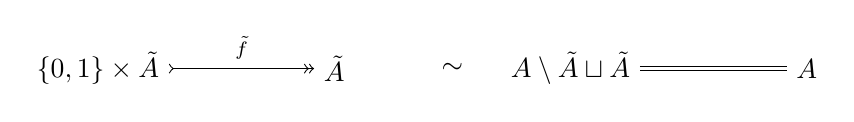
\begin{tikzpicture}[auto]
    \node (a) at (0, 0) {$\left\{ 0,1\right\} \times \tilde{A} $};
    \node (b) at (3, 0) {$\tilde{A} $};
    \node (c) at (6, 0) {$A\setminus \tilde{A} \sqcup \tilde{A} $};
    \node (d) at (9, 0) {$A$};
    \node (e) at (4.5, 0) {$\sim $};
    \draw [>->>] (a) to node {$\scriptstyle \tilde{f} $} (b);
    \draw [double distance=1pt] (c) to node {$\scriptstyle $} (d);
  \end{tikzpicture} 
\end{center}
次式のようになる。
\begin{align*}
\# A &= \# {A \setminus \widetilde{A} \sqcup \widetilde{A}}\\
&= \# \widetilde{A}\\
&= \# {\left\{ 0,1 \right\} \times \widetilde{A}}\\
&= \# \left\{ 0,1 \right\}\# \widetilde{A}\\
&= 2\# \widetilde{A}\\
&= 2\# {A \setminus \widetilde{A} \sqcup \widetilde{A}}\\
&= 2\# A
\end{align*}
ここで、$\# B \leq \# A$が成り立つなら、次式が成り立つことにより、
\begin{align*}
\# A &\leq \# A + \# B\\
&\leq \# A + \# A\\
&= 2\# A
\end{align*}
$\# A + \# B = \# A$が成り立つ。\par
その集合$A$の部分集合$A'$とこれを用いた全単射な写像$f:A' \times A'\overset{\sim}{\rightarrow}A'$の組$\left( A',f \right)$が考えられるとする。このとき、その集合$A'$が可算集合である、即ち、$\# A' = \aleph_{0}$が成り立つとき、定理\ref{1.2.7.7}より$\# \left( A' \times A' \right) = \aleph_{0}$が成り立つ、即ち、$\aleph_{0}^{2} = \aleph_{0}$が成り立つので、そのような写像$f$は存在しその組$\left( A',f \right)$は存在する。\par
ここで、そのような組$\left( A',f \right)$全体の集合を$\mathfrak{M}$とおく。その集合$\mathfrak{M}$の任意の2つの元々$\left( A',f \right)$、$\left( B',g \right)$を用いて$A' \subseteq B'$かつ$g|A' \times A' = f$が成り立つことが$\left( A',f \right)O\left( B',g \right)$と定義されるとする。このとき、上記と同様にして、その組$\left( \mathfrak{M,}O \right)$が帰納的な順序集合であることが示される。\par
したがって、Zornの補題よりその集合$\mathfrak{M}$には極大元$\left( \widetilde{A},\widetilde{f} \right)$が存在する。上記と同様にして、$\# \widetilde{A} \geq \aleph_{0}$が成り立つことが示される。ここで、$\# {A \setminus \widetilde{A}} \geq \# \widetilde{A}$が成り立つと仮定すると、$A'' \sim \widetilde{A}$なるその集合$A \setminus \widetilde{A}$の部分集合$A''$が存在するのであった。したがって、次のようになり、
\begin{align*}
\left( \widetilde{A} \sqcup A'' \right) \times \left( \widetilde{A} \sqcup A'' \right) &= \left( \left( \widetilde{A} \sqcup A'' \right) \times \widetilde{A} \right) \sqcup \left( \left( \widetilde{A} \sqcup A'' \right) \times A'' \right)\\
&= \left( \widetilde{A} \times \widetilde{A} \right) \sqcup \left( A'' \times \widetilde{A} \right) \sqcup \left( \widetilde{A} \times A'' \right) \sqcup \left( A'' \times A'' \right)
\end{align*}
ここで、次式が成り立つので、
\begin{align*}
\widetilde{A} \sim \widetilde{A} \times \widetilde{A} \sim A'' \times \widetilde{A} \sim \widetilde{A} \times A'' \sim A'' \times A''
\end{align*}
したがって、その集合$\left( A'' \times \widetilde{A} \right) \sqcup \left( \widetilde{A} \times A'' \right) \sqcup \left( A'' \times A'' \right)$を$D$とおくと、次式のようになる。
\begin{align*}
\# D &= \# {\left( A'' \times \widetilde{A} \right) \sqcup \left( \widetilde{A} \times A'' \right) \sqcup \left( A'' \times A'' \right)}\\
&= \# {A'' \times \widetilde{A}} + \# {\widetilde{A} \times A''} + \# {A'' \times A''}\\
&= \# \widetilde{A} + \# \widetilde{A} + \# \widetilde{A}\\
&= 3\# \widetilde{A} = \# \widetilde{A}
\end{align*}
これにより、全単射$g:D\overset{\sim}{\rightarrow}A''$が存在し、次式のような写像$g'$が定義されると、
\begin{align*}
g':\left( \widetilde{A} \sqcup A'' \right) \times \left( \widetilde{A} \sqcup A'' \right) \rightarrow \widetilde{A} \sqcup A'';a \mapsto \left\{ \begin{matrix}
\widetilde{f}(a) & \mathrm{if} & a \in \widetilde{A} \times \widetilde{A} \\
g(a) & \mathrm{if} & a \in D \\
\end{matrix} \right.\ 
\end{align*}
次式が成り立つことにより、
\begin{align*}
\left( \widetilde{A} \sqcup A'' \right) \times \left( \widetilde{A} \sqcup A'' \right) = \left( \widetilde{A} \times \widetilde{A} \right) \sqcup D
\end{align*}
その写像$g$は全単射である。以上より、$\widetilde{A} \subset \widetilde{A} \sqcup A''$かつ$g'|\widetilde{A} \times \widetilde{A} = \widetilde{f}$が成り立つので、$\left( \widetilde{A},\widetilde{f} \right)O\left( \widetilde{A} \sqcup A'',g' \right)$が成り立つことになる。しかしながら、これはその組$\left( \widetilde{A},\widetilde{f} \right)$がその集合$\mathfrak{M}$の極大元であることに矛盾する。したがって、$\# \left( A \setminus \widetilde{A} \right) < \# \widetilde{A}$が成り立つ。\par
したがって、上記の議論により次式のようになり、
\begin{center}
  \begin{tikzpicture}[auto] 
    \node (a) at (0, 0) {$\tilde{A} \times \tilde{A} $};
    \node (b) at (3, 0) {$\tilde{A} $};
    \node (c) at (6, 0) {$A\setminus \tilde{A} \sqcup \tilde{A} $};
    \node (d) at (9, 0) {$A$};
    \node (e) at (4.5, 0) {$\sim $};
    \draw [>->>] (a) to node {$\scriptstyle \tilde{f} $} (b);
    \draw [double distance=1pt] (c) to node {$\scriptstyle $} (d);  
  \end{tikzpicture} 
\end{center}
次のようになる。
\begin{align*}
\# A &= \# {\widetilde{A} \sqcup A \setminus \widetilde{A}}\\
&= \# \widetilde{A} + \# {A \setminus \widetilde{A}}\\
&= \# \widetilde{A}\\
&= \# {\widetilde{A} \times \widetilde{A}}\\
&= \# \widetilde{A}\# \widetilde{A}\\
&= {\# \widetilde{A}}^{2}\\
&= \left( \# \widetilde{A} + \# {A \setminus \widetilde{A}} \right)^{2}\\
&= \left( \# {\widetilde{A} \sqcup A \setminus \widetilde{A}} \right)^{2}\\
&= \left( \# A \right)^{2}
\end{align*}
ここで、$1 \leq \# B \leq \# A$が成り立つなら、次式が成り立つことにより、
\begin{align*}
\# A &\leq \# A\# B\\
&\leq \# A\# A\\
&= \left( \# A \right)^{2}
\end{align*}
$\# A\# B = \# A$が成り立つ。\par
$2 \leq \# B \leq \# A$が成り立つなら、$2^{\# A} \leq {\# B}^{\# A}$が成り立つ。ここで、$\# B < \# {\mathfrak{P}(B)}$が成り立つので、次のようになる。
\begin{align*}
{\# B}^{\# A} &\leq {\# {\mathfrak{P}(B)}}^{\# A}\\
&= \left( 2^{\# B} \right)^{\# A}\\
&= 2^{\# A\# B}
\end{align*}
ここで、$\# A\# B = \# A$が成り立つので、したがって、$2^{\# A} = {\# B}^{\# A}$が成り立つ。
\end{proof}
\begin{thebibliography}{50}
  \bibitem{1}
    松坂和夫, 集合・位相入門, 岩波書店, 1968. 新装版第2刷 p97-115,125-129 ISBM978-4-00-029871-1
\end{thebibliography}
\end{document}

\end{document}